\documentclass[11pt,a4paper]{article}
\usepackage[T1]{fontenc}
\usepackage{lmodern}
\usepackage[a4paper,margin=28mm,top=24mm,bottom=24mm]{geometry}
\usepackage{amsmath,amssymb,amsfonts,amsthm,mathtools,bm}
\usepackage{mathrsfs}
\usepackage{booktabs,longtable,array,enumitem}
\usepackage{xcolor}
\usepackage{graphicx}
\usepackage[numbers,sort&compress]{natbib}
\usepackage[hidelinks]{hyperref}
\setcitestyle{numbers,square,sort&compress}
\setcounter{tocdepth}{2}
\hypersetup{bookmarksopen=true,bookmarksdepth=2}
\newcommand{\keywords}[1]{\par\smallskip\noindent\textbf{Keywords.} #1\par}
\numberwithin{equation}{section}
\theoremstyle{plain}
\newtheorem{theorem}{Theorem}[section]
\newtheorem{lemma}[theorem]{Lemma}
\newtheorem{proposition}[theorem]{Proposition}
\newtheorem{corollary}[theorem]{Corollary}
\theoremstyle{definition}
\newtheorem{definition}[theorem]{Definition}
\theoremstyle{remark}
\newtheorem{remark}[theorem]{Remark}
\allowdisplaybreaks[2]
\setlength{\emergencystretch}{2em}
\raggedbottom
\hypersetup{
  pdftitle={A local solution of Ericksen's problem},
  pdfauthor={Jingbei Bai},
  pdfsubject={Universal deformations in incompressible isotropic elasticity},
  pdfkeywords={Universal deformation, incompressible isotropic elasticity, Ericksen problem}
}
\begin{document}
\title{A local solution of Ericksen's problem}
\author{Jingbei Bai\\
{\small Xingjian College, Tsinghua University}\\
{\small\href{mailto:bjb23@mails.tsinghua.edu.cn}{\texttt{bjb23@mails.tsinghua.edu.cn}}}}
\date{}
\maketitle
\begin{abstract}
Ericksen's problem asks for all universal deformations of homogeneous
incompressible isotropic hyperelastic solids \cite{Ericksen1954}.
Such deformations can be maintained in equilibrium, without body forces,
for every isotropic strain energy function, while the pressure and surface
tractions may depend on the constitutive law. Six classical families are
known, but their completeness has remained open for three distinct
constant principal stretches with unrestricted principal directions
\cite{YavariGoriely2023,Yavari2026Residual}. We prove that every orientation
preserving $C^3$ incompressible local universal deformation in three
dimensions belongs locally to one of these families, including their
regular Cartesian continuations.

The main step is to prove that, for constant pairwise distinct principal
stretches, the plane field orthogonal to one principal direction is locally
integrable. Using the principal frame
formulation \cite{Marris1975,Marris1982}, we reduce the universal equilibrium
and compatibility equations to a finite differential system. Removing the
length scale yields a normalized state map whose fibres of positive
dimension induce common local Euclidean similarities of the reference and
current configurations, with the same dilation factor. On a hypothetical
region where all three principal abnormalities are nonzero, analysis of
these similarities and the frame equations excludes ranks zero, one and
two. For rank three, we bound the dimension of the Zariski closure of the
state image by two, using estimates for the generic fibres of the
projection onto the two abnormality ratios.

Real analyticity follows from neo-Hookean equilibrium. It selects a fixed
principal label whose orthogonal plane field is integrable throughout a
neighbourhood, and permits continuation of the classical deformations
through critical points of the principal invariant map and removable
coordinate singularities. Kafadar's theorem \cite{Kafadar1972} and the
earlier classifications
\cite{MarrisShiau1970,MarrisShiauCorr1970,MartinCarlson1976} then establish
the completeness of the six classical families and resolve the local form
of Ericksen's problem.
\end{abstract}
\keywords{Universal deformation, incompressible isotropic elasticity, Ericksen problem}
\clearpage
\tableofcontents
\clearpage
\section{Introduction}\label{sec:introduction}

Ericksen \cite{Ericksen1954} asked which deformations of a homogeneous
incompressible isotropic elastic solid can be maintained in equilibrium,
without body forces, for every isotropic strain energy function. These
are the universal deformations. The pressure and surface tractions may
depend on the constitutive law. Material homogeneity means that this law
is independent of position. The classical examples also provide settings
for constitutive experiments \cite{RivlinSaunders1951,Saccomandi2001}.

Rivlin's work on finite bending and torsion
\cite{Rivlin1948,Rivlin1949Flexure,Rivlin1949Torsion} preceded Ericksen's
systematic classification. For unconstrained compressible isotropic
solids, Ericksen \cite{Ericksen1955} proved that every universal
deformation is homogeneous. For incompressible solids, his earlier paper
\cite{Ericksen1954} gave four inhomogeneous families in addition to the
homogeneous family. Singh and Pipkin \cite{SinghPipkin1965} subsequently
found the logarithmic cylindrical family, and Klingbeil and Shield
\cite{KlingbeilShield1966} obtained a plane special case. Fosdick
\cite{Fosdick1966} observed that a known cylindrical deformation has
constant principal invariants despite its inhomogeneity. The six
classical families therefore include deformations with constant principal
stretches and a spatially varying deformation gradient.

Ericksen's classification left two cases to be considered: repeated
principal values and constant principal invariants. The results of
Marris and Shiau \cite{MarrisShiau1970,MarrisShiauCorr1970} and Martin and
Carlson \cite{MartinCarlson1976}, together with Ericksen's analysis,
settle the classification on regular patches where at least one principal
invariant varies. Kafadar \cite{Kafadar1972} treated constant repeated
principal values. What remains is the case of three distinct constant
principal stretches, with no restriction on their principal directions.

Fixing the stretches leaves the principal frame free to vary in space.
Kafadar \cite{Kafadar1972} proved that a deformation in this remaining
case is homogeneous or logarithmic cylindrical if one principal
direction is normal to a local family of surfaces. The condition is
equivalent to the vanishing of one of the abnormalities of the principal
frame. The missing step is therefore to show that the universal equilibrium
and compatibility equations force one of the principal abnormalities
to vanish.

Marris \cite{Marris1975} studied these equations through the curvatures
and abnormalities of the principal frame. He excluded additional
solutions when two abnormalities are constant. His 1982 paper
\cite[Main Theorems~1 and~2]{Marris1982} established a homogeneous
polynomial relation among the principal value ratios and the frame
curvatures and abnormalities, and ruled out additional solutions when
the abnormality ratios are constant. The concluding discussion
\cite[pp.~171--172]{Marris1982} isolates the difficulty of obtaining
independent differential restrictions in the presence of common
polynomial factors.

Other reductions imposed a particular deformation geometry: plane
deformations with uniform transverse stretch in Fosdick and Schuler
\cite{FosdickSchuler1969}, radial symmetry in Fosdick
\cite{Fosdick1971}, and finite anti-plane shear in Knowles
\cite{Knowles1979}. Hill and Arrigo \cite{HillArrigo1999} later reduced
a constant invariant problem to coupled nonlinear partial differential
equations. An account of these questions within the theory of universal
solutions and relations is given by Saccomandi \cite{Saccomandi2001}.

More recent work has considered anelasticity
\cite{YavariGoriely2016,Goodbrake2020}, anisotropy
\cite{YavariGoriely2021}, and material inhomogeneity
\cite{Yavari2021,YavariGoriely2023}.
Goodbrake, Yavari and Goriely \cite{Goodbrake2020} formulated the
problem geometrically and identified the Lie subgroup symmetries of the
six known families. The universal deformations of isotropic Cauchy
elasticity and hyperelasticity were shown to coincide by Yavari
\cite{Yavari2024}. Related studies concern implicit constitutive
equations \cite{YavariGoriely2024Implicit}, the geometry of nonlinear
Cauchy elasticity \cite{YavariGoriely2025}, and residual stress
\cite{YavariMerodioShariff2025,Yavari2026Residual}.
Motaghian and Yavari \cite{MotaghianYavari2026} extended the equivalence
of universality constraints to transversely isotropic, orthotropic and
monoclinic Cauchy elastic solids.

We prove that every $C^3$ universal deformation with three distinct
constant principal stretches has, near each point, a fixed principal
direction normal to a family of surfaces
(Theorem~\ref{completion:zerocontact}). Kafadar's theorem
\cite{Kafadar1972} then gives the homogeneous
and logarithmic cylindrical families. Combined with the earlier
classifications
\cite{Ericksen1954,MarrisShiau1970,MarrisShiauCorr1970,MartinCarlson1976},
this establishes the local $C^3$ classification into the six classical
families (Theorem~\ref{intro:main}).

The proof starts from the principal frame equations
\cite{Marris1975,Marris1982}. We adjoin the derivatives needed to close
these equations and use their weighted homogeneity to remove the length
scale. This gives a normalized state map on a hypothetical region where
all three abnormalities are nonzero. Its fibres determine common local
Euclidean similarities of the reference and current configurations,
with the same dilation factor (Proposition~\ref{fnd:symmetry}).
Ranks zero and one yield at least two independent infinitesimal
similarities; rank two yields one. Their classification and the frame
equations exclude all three ranks.

At rank three, the normalized state distinguishes nearby points.
We estimate the dimension of its Zariski closure by projection onto the
two abnormality ratios. Their image cannot be a point. Over the whole
ratio plane the generic fibre is finite; over a ratio curve it has
dimension at most one. In either case the state image has dimension
at most two (Theorem~\ref{r3:theorem}), contradicting rank three.
The fibre estimates use a weighted projective completion. Normal
compatibility equations exclude a boundary point when every incident
arc is forced to remain at infinity. On the remaining boundary family,
the induced differential equations have no algebraic solutions.

Equilibrium for a neo-Hookean material gives a properly elliptic
system, so analytic interior regularity
\cite[Theorem~6.8.1]{Morrey1966} applies to the $C^3$ deformation.
Analyticity selects a fixed principal label with an integrable
orthogonal plane field throughout a neighbourhood. It also continues
the classical models through critical points of the principal invariant
map and removable coordinate singularities
(Proposition~\ref{completion:continuation}). This includes their regular
Cartesian continuations. Direct equilibrium calculations for arbitrary
strain energies prove the converse.

\paragraph{Organization of the paper.}
Section~\ref{sec:geometry} states the main results, records the six
classical models, and derives the geometric equations.
Section~\ref{sec:normalization} constructs the normalized state map and
identifies its fibres with common similarities.
Section~\ref{sec:lowranks} excludes ranks zero and one;
Sections~\ref{sec:similarity}--\ref{sec:dilation} exclude rank two.
Section~\ref{sec:rankthree} proves the algebraic dimension bound, and
Section~\ref{sec:completion} completes the classification, continuation
and converse arguments. Section~\ref{sec:conclusion} discusses global
realizations and the classification of material preferred directions.
Appendices~A--E contain the supporting
geometric and algebraic arguments. The polynomial coefficient matrix
for the linear equations is given in Supplement~\ref{supp:momentcoefficients}.

\section{Universal deformations and the geometric equations}\label{fnd:secgeometry}\label{sec:geometry}

\subsection{Universal deformations and the main results}\label{sec:problem}

Let $\Omega\subset\mathbb R^3$ be a Euclidean domain and let
$\chi:\Omega\to\mathbb R^3$ be an orientation preserving $C^3$ local
diffeomorphism. Write
\begin{equation}\label{intro:kinematics}
 F=D\chi,\qquad \det F=1,\qquad
 B=FF^{\top},\qquad c=B^{-1},\qquad
 I_1=\operatorname{tr}B,\quad I_2=\operatorname{tr}c.
\end{equation}
Let $g$ denote the spatial Euclidean metric and $\mathrm{vol}_g$ its
oriented volume form.
Here $B$ is the left Cauchy--Green tensor and $c$ is the spatial metric
induced by the inverse deformation, called the Cauchy deformation tensor
in \cite{Kafadar1972}. Spatial tensors are defined on each
local inverse chart. Their invariants are pulled back to $\Omega$ when
a statement concerns a connected reference domain.
The principal values of $B$ are its eigenvalues and are the squares of
the principal stretches. Marris and Shiau use the term ``proper values''
for eigenvalues \cite{MarrisShiau1970}. The principal values of $c$ are
their reciprocals. Positivity, constancy and pairwise distinctness are
equivalent for these two triples of values and for the principal stretches.

The deformation is \emph{universal} if, for every sufficiently smooth
strain energy $W(I_1,I_2)$, there is a local pressure $p_W$ such that
\begin{equation}\label{intro:stress}
 T_W=-p_W I+2W_1B-2W_2c,\qquad \operatorname{div}T_W=0.
\end{equation}
Body forces are absent. The pressure and the required surface traction
may depend on $W$. Here $W_i=\partial W/\partial I_i$, and
all derivatives in \eqref{intro:stress} are spatial.

Following the principal frame formulation in
\cite{Marris1975,Marris1982}, choose on a chart with distinct principal
values an oriented orthonormal principal frame $(e_1,e_2,e_3)$ with dual
coframe $(\alpha_1,\alpha_2,\alpha_3)$. Write
$h_i=e_i\cdot\operatorname{curl}e_i$ for the abnormality of $e_i$
\cite[p.~112]{Marris1975}. The identity
$\alpha_i\wedge d\alpha_i=h_i\,\mathrm{vol}_g$ shows that $h_i=0$
precisely when the two dimensional plane field orthogonal to $e_i$
is integrable. Equivalently, $e_i$ is normal to a local family of
surfaces. All references to integrability below concern this plane
field.

\begin{theorem}[A principal direction normal to surfaces]
\label{completion:zerocontact}
Let a $C^3$ local universal deformation have constant, positive,
pairwise distinct principal values. Every spatial point has a connected
ball neighbourhood on which a fixed principal label $i$ satisfies
\[
 h_i\equiv0.
\]
Equivalently, that principal direction is normal to a local family of
surfaces.
\end{theorem}

This theorem supplies Kafadar's geometric hypothesis. Its proof occupies
Sections~\ref{sec:geometry}--\ref{sec:rankthree} and is concluded in
Section~\ref{sec:completion}. Together with the classical classifications
it gives the following theorem. Here $\mathcal F_0$ denotes the
homogeneous family and $\mathcal F_5$ the logarithmic cylindrical
family. All six models are defined in the next subsection.

\begin{theorem}[Local classification]\label{intro:main}
Every $C^3$, orientation preserving, incompressible local universal
deformation in three dimensions is locally one of
$\mathcal F_0,\ldots,\mathcal F_5$ with the parameter restrictions in
Section~\ref{sec:classicalmodels}, including their regular Cartesian
continuations. Conversely, each
listed model is locally universal wherever it is a regular deformation.
\end{theorem}

\subsection{The classical deformations}\label{sec:classicalmodels}

The models $\mathcal F_0,\ldots,\mathcal F_4$ are those of Ericksen
\cite{Ericksen1954}. The logarithmic cylindrical model $\mathcal F_5$
is due to Singh and Pipkin \cite{SinghPipkin1965}; Klingbeil and Shield
\cite{KlingbeilShield1966} obtained a plane special case.
We use the conventional mechanical descriptions in
\cite[\S1]{YavariGoriely2023}. Uppercase cylindrical coordinates $(R,\Theta,Z)$ refer to
the reference configuration, and lowercase coordinates $(r,\theta,z)$ to
the current configuration. Angles are local coordinates on a sector.
Fixed Euclidean coordinate changes and additive coordinate constants are
understood. The parameter restrictions below impose the signed Jacobian
$\det D\chi=1$.

\begin{description}
\item[$\mathcal F_0$.] Homogeneous deformations:
\begin{equation}\label{intro:family0}
 \chi(X)=LX+b_0,\qquad L\in\mathrm{SL}(3,\mathbb R).
\end{equation}
\item[$\mathcal F_1$.] Bending, stretching and shearing of a rectangular block:
\begin{equation}\label{intro:family1}
 r^2=2\alpha X+d,\qquad \theta=\beta Y+\theta_0,\qquad
 z=(\alpha\beta)^{-1}Z+\gamma Y+z_0,\qquad \alpha\beta\ne0.
\end{equation}
The displayed cylindrical chart requires $r>0$.
\item[$\mathcal F_2$.] Straightening, stretching and shearing of a sector of a cylindrical shell:
\begin{equation}\label{intro:family2}
 \begin{gathered}
 x=\tfrac\alpha2R^2+x_0,\qquad y=\beta\Theta+y_0,\\
 z=(\alpha\beta)^{-1}Z+\gamma\Theta+z_0,\qquad \alpha\beta\ne0,\quad R>0.
 \end{gathered}
\end{equation}
\item[$\mathcal F_3$.] Inflation, bending, torsion, extension and shearing
of an annular wedge:
\begin{equation}\label{intro:family3}
 \begin{aligned}
 r^2&=AR^2+B_0,&\theta&=k\Theta+\delta Z+\theta_0,\\
 z&=\kappa\Theta+\gamma Z+z_0,& A(k\gamma-\delta\kappa)&=1,
 \end{aligned}\qquad R,r>0.
\end{equation}
All parameters in this model are constants; $A$ is its radial coefficient.
\item[$\mathcal F_4$.] Inflation and inversion of a spherical shell,
including reversal of the
radial direction with the compensating angular orientation:
\begin{equation}\label{intro:family4}
 \begin{gathered}
 \chi(P+Rn)=Q_0+r(R)Qn,\qquad r^3=\varepsilon R^3+B_0,\\
 \varepsilon=\det Q,\quad Q\in\mathrm O(3),\quad |n|=1.
 \end{gathered}
\end{equation}
Both radii are positive in this expression.
\item[$\mathcal F_5$.] Inflation, bending, extension and azimuthal shearing
of an annular wedge, with constant invariants (the logarithmic cylindrical family):
\begin{equation}\label{intro:family5}
 \begin{gathered}
 r=\alpha R,\qquad \theta=\beta\log R+k\Theta+\theta_0,\\
 z=\gamma Z+z_0,\qquad
 \alpha>0,\quad \alpha^2k\gamma=1,\quad R>0.
 \end{gathered}
\end{equation}
Its plane deformation gradient in orthonormal cylindrical bases has the
constant block $\alpha\left(\begin{smallmatrix}1&0\\\beta&k\end{smallmatrix}\right)$.
Consequently the principal stretches are constant although the Cartesian
gradient usually is not. Either planar value may coincide with the axial value.
\end{description}

The families overlap at special parameters. At an interior axis or
centre, a model means its regular Cartesian continuation when one exists.
The continuations are described in Section~\ref{completion:continuationsection}.

The remainder of this section develops the geometric equations
needed to prove Theorem~\ref{completion:zerocontact}. The principal
values are fixed, while the principal frame may vary.

\subsection{Equilibrium for constant principal values}
When the principal invariants are constant, $W_1,W_2$ are spatial
constants. Taking $W=I_1/2$ and $W=I_2/2$ gives the necessary conditions
\begin{equation}\label{fnd:constanteq}
d(\operatorname{div}B)^\flat=d(\operatorname{div}c)^\flat=0.
\end{equation}
Conversely, linear combinations of the local pressure potentials in
\eqref{fnd:constanteq} give equilibrium for every strain energy $W$. Thus
these conditions are also sufficient.
The inverse deformation $f=\chi^{-1}$ satisfies $c=f^*g_{\mathrm{ref}}$. Conversely, a positive flat metric $c$ of determinant one has an orientation preserving local Euclidean development $f$, with $\det Df=1$. Thus the local problem with constant invariants is
\begin{equation}\label{fnd:twometric}
c>0,\quad \det c=1,\quad \operatorname{spec}_g c\text{ constant},\quad
\operatorname{Riem}(c)=0,\quad \eqref{fnd:constanteq}.
\end{equation}
Flatness is a compatibility equation independent of the two pressure equations.

\subsection{Interior analyticity}
Universality includes equilibrium for the neo-Hookean energy. The
following interior regularity result therefore applies.

\begin{lemma}\label{fnd:analyticity}
Every $C^3$ incompressible local diffeomorphism in equilibrium for the
neo-Hookean energy is real analytic. In particular, a $C^3$ universal
deformation and each of its local inverses are real analytic.
\end{lemma}
\begin{proof}
Use reference Cartesian coordinates $X_A$, put $\mathsf A_\chi=\operatorname{cof}F$, and select the energy $W(F)=|F|^2/2$. The spatial pressure $p_W$ has pullback $p_W\circ\chi$ to the reference domain. The Piola identity gives
\begin{equation}\label{fnd:neo}
\Delta\chi_i=(\mathsf A_\chi)_{iA}\partial_A(p_W\circ\chi),\qquad \det F=1,\qquad
\nabla(p_W\circ\chi)=F^{\top}\Delta\chi.
\end{equation}
Since $\chi\in C^3$, the last expression is $C^1$ and $p_W\circ\chi$ is $C^2$. Applying the reference Laplacian to $\det F=1$ and substituting the first equation gives
\begin{equation}\label{fnd:pressureelliptic}
(\mathsf A_\chi^{\top}\mathsf A_\chi)_{AB}\partial_{AB}(p_W\circ\chi)
+(\mathsf A_\chi)_{iA}(\partial_A(\mathsf A_\chi)_{iB})\partial_B(p_W\circ\chi)
+\sum_C D^2\det(F)[\partial_CF,\partial_CF]=0.
\end{equation}
The three equations for $\chi$ and \eqref{fnd:pressureelliptic} form a second-order nonlinear analytic system for $\chi,p_W\circ\chi$, with coefficients polynomial in their first and second derivatives.

The principal symbol of its linearization has the triangular form
\[
L(\xi)=\begin{pmatrix}|\xi|^2I_3&0\\ K(\xi)&\xi^{\top}\mathsf A_\chi^{\top}\mathsf A_\chi\xi\end{pmatrix},
\qquad \det L(\xi)=|\xi|^6|\mathsf A_\chi\xi|^2>0\quad(\xi\ne0).
\]
The row $K$ consists of the second-order variations of $\chi$ in the pressure equation. For independent real $\xi,\eta$, each of the positive quadratic factors in $\det L(\xi+z\eta)$ has one root in each half-plane. Counting multiplicity gives four roots in each half-plane, so the system is properly elliptic. Take equation weights zero and unknown weights two. The solution $(\chi,p_W\circ\chi)$ is $C^2$, and the equations are polynomial in its derivatives. Morrey's interior regularity theorem \cite[Theorem~6.8.1, pp.~277--278]{Morrey1966} first gives smoothness and, in its analytic case, real analyticity of $\chi,p_W\circ\chi$. The analytic inverse function theorem makes each local inverse analytic, and composition with it gives analyticity of the spatial pressure $p_W$.
\end{proof}

On the reference domain the invariants are represented by $|F|^2$ and $|\mathsf A_\chi|^2$, so they are analytic. On a connected domain, constancy on a nonempty open subset extends to the whole domain by the analytic identity theorem.

\subsection{The equations in a principal frame}
We use the principal frame formulation of Marris
\cite{Marris1975,Marris1982}.
We now restrict to constant, positive, pairwise distinct principal values. Normalize the eigenvalues of $B$ by a common constant factor to $(1,a,b)$, where
\begin{equation}\label{fnd:materialdomain}
a,b>0,\qquad (a-1)(b-1)(a-b)\ne0.
\end{equation}
The physical eigenvalues of $B$, with product one, are
$(ab)^{-1/3}(1,a,b)$. Constant rescaling does not affect flatness
or closedness of tensor divergence, so the metric weight vectors are $(1,1,1)$ and $(1,1/a,1/b)$. Write $\lambda_i$ for the principal values of the physical metric $c=B^{-1}$; thus
\[
 (\lambda_1,\lambda_2,\lambda_3)=(ab)^{1/3}(1,a^{-1},b^{-1}),
 \qquad c=\sum_i\lambda_i\alpha_i^2.
\]
All orderings of the principal values are allowed. The parameters
$a,b$ are fixed ratios of principal values.

Choose the oriented principal frame and its dual coframe as in
Section~\ref{sec:problem}, and put $P_i=e_i\otimes e_i$.
Define the frame coefficients and directional derivatives by
\begin{equation}\label{intro:contact}
 p_{ij}=e_j\cdot\operatorname{curl}e_i,\qquad
 h_i=p_{ii},\qquad D_i=e_i\cdot\nabla.
\end{equation}

The matrix whose rows are $(1,1,1)$, $(1,a,b)$ and $(1,1/a,1/b)$ is invertible on \eqref{fnd:materialdomain}. Since $\sum P_i=I$, the two pressure equations are equivalent to
\begin{equation}\label{fnd:projectors}
\operatorname{div}P_i=\nabla\phi_i,\qquad \sum_i\phi_i=0.
\end{equation}
Indeed, its determinant is a nonzero Vandermonde factor divided by $ab$. For a unit vector field $e$,
\[
\operatorname{div}(e\otimes e)=(\operatorname{div}e)e-e\times\operatorname{curl}e.
\]
Its component perpendicular to $e_i$ therefore gives
\begin{equation}\label{fnd:pressureframe}
\begin{gathered}
\operatorname{curl}e_i=h_ie_i+e_i\times\nabla\phi_i,
\qquad \vartheta_i=e^{\phi_i}\alpha_i,\\
\kappa_i=e^{2\phi_i}h_i,\qquad
d\vartheta_i=\kappa_i\vartheta_j\wedge\vartheta_k
\end{gathered}
\end{equation}
for cyclic $(i,j,k)$, with $\alpha_i\wedge d\alpha_i=h_i\,\mathrm{vol}_g$.

To combine the pressure equations with flatness, we express both systems
in the same principal frame \cite{Marris1982}. Let $\epsilon_{ijk}$ be the alternating
symbol. The structure coefficients and the Levi--Civita connection of
a constant diagonal frame metric of weights $w$ are
\begin{equation}\label{fnd:koszul}
C^k_{ij}=-\sum_\ell\epsilon_{ij\ell}p_{k\ell},\qquad
\Gamma^k_{ij}(w)=\frac{w_kC^k_{ij}-w_iC^i_{jk}+w_jC^j_{ki}}{2w_k}.
\end{equation}
With the first lower index indicating differentiation, the curvature is
\begin{equation}\label{fnd:curvature}
R^\ell{}_{kij}(w)=D_i\Gamma^\ell_{jk}-D_j\Gamma^\ell_{ik}
+\sum_m(\Gamma^m_{jk}\Gamma^\ell_{im}-\Gamma^m_{ik}\Gamma^\ell_{jm}-C^m_{ij}\Gamma^\ell_{mk}).
\end{equation}
For $w$ constant define
\[
A_i(w)=(w_i-w_j)p_{jk}-(w_i-w_k)p_{kj}\quad ((i,j,k)\text{ cyclic}).
\]
These are the frame components of $\operatorname{div}(\sum w_iP_i)$, and its curl components are
\begin{equation}\label{fnd:curlsource}
D_jA_k(w)-D_kA_j(w)+\sum_\ell A_\ell(w)p_{\ell i}.
\end{equation}

\subsection{Finite closure of the frame equations}

The curvature expressions \eqref{fnd:curvature} and the pressure
expressions \eqref{fnd:curlsource} are linear in the first derivatives
of $p_{ij}$, with quadratic terms in the coefficients themselves.
Their combined linear system therefore determines which derivatives
must be retained as independent state coordinates. Commutator
identities then determine the additional derivatives needed for closure.

The curvature and pressure equations determine the derivatives of the
nine frame coefficients up to six functions. Two prolongations determine
their further derivatives up to two additional functions. The resulting
system has seventeen coordinates. The construction and residual equations
are given in Appendix~\ref{appf:finiteconstruction}.

The six first derivative coordinates are
\begin{equation}\label{fnd:freejets}
(\tau_0,\tau_1,\tau_2,\tau_3,\tau_4,\tau_5)
=(D_2p_{23},D_3p_{13},D_3p_{22},D_3p_{23},D_3p_{31},D_3p_{32}).
\end{equation}
The two remaining coordinates are $u_0=D_3\tau_0$ and $u_1=D_3\tau_2$.
The state is
\begin{equation}\label{fnd:17state}
\mathsf S=(p_{11},p_{12},p_{13},p_{21},p_{22},p_{23},p_{31},p_{32},p_{33},\tau_0,\ldots,\tau_5,u_0,u_1).
\end{equation}
We write $\boldsymbol p=(p_{ij})$,
$\boldsymbol\tau=(\tau_0,\ldots,\tau_5)^{\top}$ and
$\boldsymbol u=(u_0,u_1)^{\top}$ for the three coordinate blocks,
with the matrix entries ordered by rows as in \eqref{fnd:17state}.

The corresponding coordinate components of its three fields are denoted
by $\mathcal Q_i^{p_{rs}}$, $\mathcal Q_i^{\tau_r}$ and
$\mathcal Q_i^{u_r}$. They are the rational functions
defined by the three successive linear systems in the appendix. The
denominators are powers of
\begin{equation}\label{fnd:guard}
P_{\mathrm{mat}}=ab(a-1)(b-1)(a-b).
\end{equation}
They are nonzero throughout the principal value domain
\eqref{fnd:materialdomain}.

\begin{proposition}[Finite differential system]\label{fnd:finiteclosure}
Every solution of \eqref{fnd:twometric} satisfies
$D_i\mathsf S=\mathcal Q_i(\mathsf S)$. With coordinate weights
$(d_1,\ldots,d_{17})=(1^9,2^6,3^2)$, the component $\mathcal Q_i^\ell$ has weight $d_\ell+1$.
The three cubic residuals, the twenty-one quartic residuals and the
bracket defects, together with all their iterated derivatives under
the $\mathcal Q_i$, vanish on every solution.
\end{proposition}
\begin{proof}
The first linear system is obtained from the two curvature tensors and
the two pressure equations. The next two systems impose the commutator
identities for the frame coefficients and the six coordinates $\tau_r$.
Their determinants are nonzero on \eqref{fnd:materialdomain}; see
\eqref{fnd:firstminor}, \eqref{fnd:secondminor} and
\eqref{appf:minor2}. Substitution into the unselected rows gives the
stated residuals. Their weights follow from the curvature equations
and the fact that directional differentiation increases weight by one.
\end{proof}

Thus the state at one point, together with an initial principal frame,
determines its evolution along each principal curve by an ordinary
differential equation. Agreement between these evolutions in different
directions is imposed by the residual equations and the bracket identities.

For a nonzero signed length scale $\ell$, write
\begin{equation}\label{fnd:weighted-state}
\mathsf S^{[\ell]}=
(\ell\boldsymbol p,\ell^2\boldsymbol\tau,\ell^3\boldsymbol u).
\end{equation}
Its coordinates are denoted by $p_{ij}^{[\ell]}$, $\tau_r^{[\ell]}$
and $u_r^{[\ell]}$. Coordinates without a superscript refer to the
unscaled state.

Let $\mathscr I_{\mathrm{raw}}$ be the ideal in
$\mathbb Q[a,b,P_{\mathrm{mat}}^{-1}][\mathsf S]$ generated by the cubic and quartic
residuals, the components of
\begin{equation}\label{fnd:bracketdefects}
\mathcal B_{ij}=\mathcal Q_i(\mathcal Q_j)-\mathcal Q_j(\mathcal Q_i)
-\sum_kC^k_{ij}\mathcal Q_k,
\end{equation}
and all their iterated derivatives under $\mathcal Q_i$. Thus
$\mathcal Q_i\mathscr I_{\mathrm{raw}}\subset\mathscr I_{\mathrm{raw}}$.
The coefficient ring is Noetherian, so this ideal has a finite generating
family.

\subsection{Reconstruction and linearization}
\begin{proposition}\label{fnd:reconstruction}
Fix an admissible triple of principal values. Suppose a local real state
set is invariant under the local flows of the three fields $\mathcal Q_i$.
On it, suppose the curvature expressions \eqref{fnd:curvature} vanish for
$w=(1,1,1)$ and $w=(1,1/a,1/b)$, the pressure expressions
\eqref{fnd:curlsource} vanish for $w=(1,1/a,1/b)$ and $w=(1,a,b)$,
and the bracket defects \eqref{fnd:bracketdefects} vanish.
Then each point of that set has a local frame realization and a
corresponding incompressible universal deformation. It suffices
that the state set be the real zero set of a finitely generated ideal
preserved by all three derivations and containing these relations.
\end{proposition}
\begin{proof}
Write $\Gamma_i(\mathsf S)=(\Gamma^k_{ij}(1,1,1))_{k,j}$, so $\Gamma_i\in\mathfrak{so}(3)$, and set $\Gamma(v,\mathsf S)=\sum_i v_i\Gamma_i(\mathsf S)$. Let $\mathbf E\in\mathrm{SO}(3)$ be the matrix whose columns are the principal vectors in Cartesian coordinates. On the ambient space $\mathbb R^{17}\times\mathrm{SO}(3)$ define
\[
L_i=\mathcal Q_i+(\mathbf E\mapsto\mathbf E\Gamma_i),\qquad \mathcal L_a=\sum_i\mathbf E_{ai}L_i.
\]
The bracket identities and Euclidean flatness give $[L_i,L_j]=\sum C^k_{ij}L_k$. The torsion-free and metric compatibility identities
\[
\Gamma^k_{ij}-\Gamma^k_{ji}=C^k_{ij},\qquad
\Gamma^k_{ij}=-\Gamma^j_{ik}
\]
then give $[\mathcal L_a,\mathcal L_b]=0$ along the invariant state set by direct expansion. Composing their ambient flows from a point of this set with parameters $x_a$ yields $\mathsf S(x),\mathbf E(x)$ and $e_i=\sum_a\mathbf E_{ai}\partial_{x_a}$. Since $\sum_a\mathbf E_{ai}\mathcal L_a=L_i$, one has $D_i\mathsf S=\mathcal Q_i$ and $D_i\mathbf E=\mathbf E\Gamma_i$. Its coframe satisfies $*d\alpha_i=\sum_jp_{ij}\alpha_j$, as required.

The second metric is positive and flat, and hence develops locally into Euclidean space. Restoring the constant determinant normalization gives the required inverse deformation; \eqref{fnd:constanteq} supplies the pressure for every energy.

For the ideal formulation, let $\mathbf q$ be a finite vector of generators.
Differential preservation gives $\mathcal Q_i\mathbf q=A_i(\mathsf S)\mathbf q$.
Along each flow, $\mathbf q$ solves a homogeneous linear ordinary
differential equation, so its zero set is invariant. The lifted flows
preserve this zero set, where the Cartesian fields $\mathcal L_a$ commute
by the same bracket identity.
\end{proof}
\begin{lemma}[Linearized reconstruction]
\label{fnd:linearized-reconstruction}
At a state of a solution, tangent vectors annihilating the differentials
of $\mathscr I_{\mathrm{raw}}$ correspond to germs satisfying the
linearized frame equations and the equations for the two metrics, with
initial frames and development origins fixed. At order $m$, states
satisfying $\mathscr I_{\mathrm{raw}}$ modulo $\epsilon^{m+1}$ correspond
to formal frame realizations over $\mathbb R[\epsilon]/(\epsilon^{m+1})$.
\end{lemma}
\begin{proof}
For first order work over $\mathbb R[\epsilon]/(\epsilon^2)$.
A state $\mathsf S+\epsilon v$ annihilates every generator of $\mathscr I_{\mathrm{raw}}$ precisely when
the relations vanish at $\mathsf S$ and their differentials annihilate $v$.
The lift and Cartesian combinations in the proof of
Proposition~\ref{fnd:reconstruction} are algebraic operations on the
state, frame, and their derivatives.  The torsion, curvature, and
bracket identities consequently make those Cartesian fields commute
also modulo $\epsilon^2$.  Their flows are constructed by solving the
ordinary real flow and its inhomogeneous linear variational equations.
Commutation supplies compatibility in all physical directions and
therefore a germ of a linearized frame realization.  Developing the
second flat metric gives the linearized deformation.  Conversely,
differentiating a germ of the original equations annihilates every
relation in $\mathscr I_{\mathrm{raw}}$. Initial translations and rotations are
the development gauges. Replacing $\epsilon^2$ by $\epsilon^{m+1}$ and
solving successive linear variational equations proves the order-$m$
statement.
\end{proof}

\section{Normalized states and common similarities}\label{fnd:secnormalization}\label{sec:normalization}

On a solution with $h_1h_2h_3\ne0$, weighted homogeneity removes one
scale and the residual equations determine five further coordinates of
$\mathsf S$. The resulting eleven coordinates define the normalized
state map $\mathsf X$.

\subsection{The normalized state}
Put
\[
\Delta_a=a(b-1),\qquad \Delta_b=b(a-1),\qquad \Delta_{ab}=a-b.
\]
The cubic residuals in Appendix~\ref{appn:cubicreconstruction} are linear in the coordinates $\tau_r$.

Define
\begin{equation}\label{fnd:mu}
\mu_1=\Delta_{ab}\left(\frac{h_3}{\Delta_b}-\frac{h_2}{\Delta_a}\right),\qquad
\mu_2=h_1-\frac{\Delta_{ab}h_3}{\Delta_b},\qquad
\mu_3=-h_1-\frac{\Delta_{ab}h_2}{\Delta_a}.
\end{equation}
In the cubic coefficient matrix, the columns belonging to $(\tau_4,\tau_5,\tau_0)$ are respectively $(\mu_1,0,0)^{\top}$, $(0,\mu_2,0)^{\top}$, $(0,0,\mu_3)^{\top}$. Consequently these three coordinates have a unique rational reconstruction wherever $\mu_1\mu_2\mu_3\ne0$.

The remaining two coordinates are recovered by the combined left
inverse \eqref{fnd:uleftinverse}. Its product with the coefficient matrix
is $7\Delta_bh_1h_2\operatorname{Id}_2$, where $\operatorname{Id}_2$ is the
two by two identity matrix.
The construction is given in Appendix~\ref{appn:cubicreconstruction}.

Normalize the state coordinates by their weights. Write
$\widehat p_{ij}=p_{ij}/h_1$,
$\widehat\tau_j=\tau_j/h_1^2$, and
$\widehat u_j=u_j/h_1^3$, and put
$\widehat h_i=h_i/h_1$. Thus $\widehat p_{ii}=\widehat h_i$ and
$\widehat p_{11}=\widehat h_1=1$.
The normalized coefficient matrix is
$\widehat{\boldsymbol p}=(\widehat p_{ij})$.
The retained coordinate map is
\begin{equation}\label{fnd:X}
\mathsf X=\left(\widehat p_{12},\widehat p_{13},\widehat p_{21},
\widehat p_{22},\widehat p_{23},\widehat p_{31},\widehat p_{32},\widehat p_{33},
\widehat\tau_1,\widehat\tau_2,\widehat\tau_3\right).
\end{equation}
These are eight normalized frame coefficients and the three retained
derivative coordinates $\widehat\tau_1,\widehat\tau_2,\widehat\tau_3$.
The map itself is smooth wherever $h_1\ne0$. On the domain
\begin{equation}\label{fnd:protected}
h_1h_2h_3\mu_1\mu_2\mu_3\ne0
\end{equation}
the preceding triangular reconstruction defines all normalized coordinates $\widehat{\mathsf S}_\ell=\mathsf S_\ell/h_1^{d_\ell}$ as rational functions of $\mathsf X$. The spatial scale is $h_1$.

Let $E_i=D_i/h_1$ and define
\[
 s_i(\mathsf X)=\mathcal Q_i^{p_{11}}(\widehat{\mathsf S}(\mathsf X)).
\]
For each retained coordinate $\widehat{\mathsf S}_\ell$ in \eqref{fnd:X},
the corresponding component of $\mathcal V_i$ is
\begin{equation}\label{fnd:normalizedfields}
 \mathcal Q_i^\ell(\widehat{\mathsf S}(\mathsf X))-
 d_\ell\widehat{\mathsf S}_\ell(\mathsf X)s_i(\mathsf X).
\end{equation}
Weighted homogeneity gives, on every solution,
\begin{equation}\label{fnd:actualnormalized}
E_i\mathsf X=\mathcal V_i(\mathsf X),\qquad E_i\log|h_1|=s_i(\mathsf X),\qquad
[E_i,E_j]=\sum_k\widetilde C^k_{ij}(\mathsf X)E_k,
\end{equation}
where $\widetilde C^k_{ij}=C^k_{ij}/h_1-s_i\delta_{jk}+s_j\delta_{ik}$.

Figure~\ref{fig:state-relations} shows these coordinate maps.
The isometry states in Section~\ref{sec:isometries} augment
$\mathsf S$ with prescribed motion data. The rank three reduction
in Section~\ref{sec:rankthree} uses an invertible rational change
of the retained coordinates.
\begin{figure}[htbp]
\centering
\setlength{\unitlength}{0.01\linewidth}
\begin{picture}(100,66)
\put(0,0){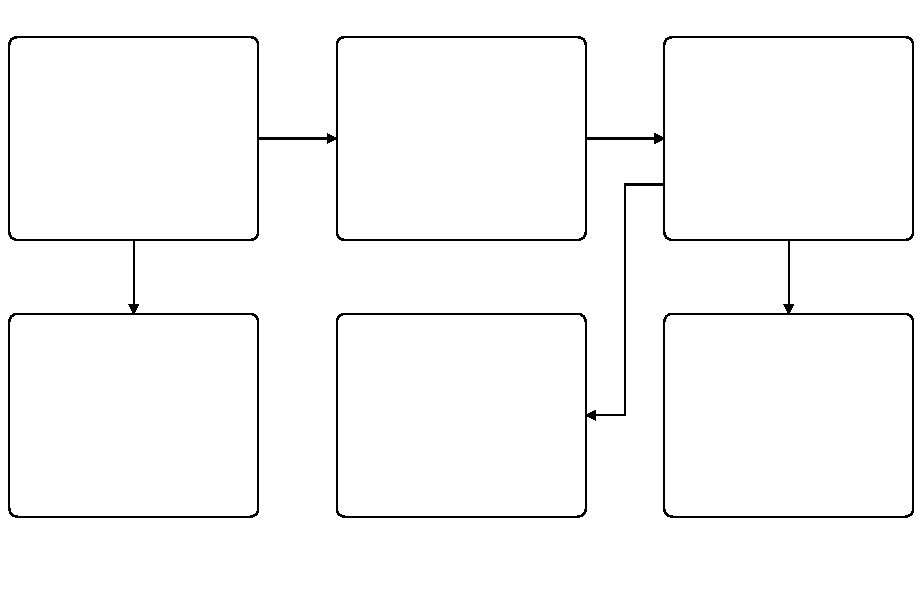
\includegraphics[width=\linewidth]{figures/state_relations_geometry.pdf}}
\put(14.500,51.000){\makebox(0,0){\parbox{25.000\unitlength}{\centering\fontsize{9.0}{11.2}\selectfont Unnormalized state $\mathsf S$\\$(p_{ij},\tau_j,u_j)$\\$9+6+2=17$ coordinates}}}
\put(50.000,51.000){\makebox(0,0){\parbox{25.000\unitlength}{\centering\fontsize{9.0}{11.2}\selectfont Full state $\widehat{\mathsf S}$\\$\widehat p_{11}=1$\\16 normalized coordinates}}}
\put(85.500,51.000){\makebox(0,0){\parbox{25.000\unitlength}{\centering\fontsize{9.0}{11.2}\selectfont Retained state $\mathsf X$\\Frame and derivative data\\$8+3=11$ coordinates}}}
\put(32.250,58.000){\makebox(0,0){\parbox{10.000\unitlength}{\centering\fontsize{8.0}{10.0}\selectfont $h_1\ne0$}}}
\put(67.750,58.000){\makebox(0,0){\parbox{10.000\unitlength}{\centering\fontsize{7.6}{9.5}\selectfont Eliminate}}}
\put(50.000,3.500){\makebox(0,0){\parbox{96.000\unitlength}{\centering\fontsize{9.0}{11.2}\selectfont $\widehat p_{ij}=p_{ij}/h_1,\quad\widehat\tau_j=\tau_j/h_1^2,\quad\widehat u_j=u_j/h_1^3$}}}
\put(50.000,21.000){\makebox(0,0){\parbox{25.000\unitlength}{\centering\fontsize{8.7}{10.9}\selectfont Reconstructed from $\mathsf X$\\$\widehat\tau_4,\widehat\tau_5,\widehat\tau_0$\\$\widehat u_0,\widehat u_1$}}}
\put(85.500,21.000){\makebox(0,0){\parbox{25.000\unitlength}{\centering\fontsize{8.4}{10.5}\selectfont Rank three coordinates\\$(\eta,\zeta,\widehat p_{ij},\mathsf R_i)$\\Invertible rational change}}}
\put(50.000,36.000){\makebox(0,0){\parbox{60.000\unitlength}{\centering\fontsize{9.0}{11.2}\selectfont $h_1h_2h_3\mu_1\mu_2\mu_3\ne0$}}}
\put(14.500,21.000){\makebox(0,0){\parbox{25.000\unitlength}{\centering\fontsize{8.7}{10.9}\selectfont Augmented state $\mathsf U$\\Unnormalized state plus\\Killing and angular data}}}
\end{picture}
\caption{The state coordinates under weighted normalization, reconstruction and the rational change in Section~\ref{sec:rankthree}. The augmented state $\mathsf U$ incorporates Killing and angular data.}
\label{fig:state-relations}
\end{figure}

\subsection{Nonconstancy of the ratios}\label{fnd:ratiosubsection}
The frame equations imply that the two ratios of abnormalities cannot
both be constant.

\begin{lemma}\label{fnd:constantratio}
For principal values satisfying \eqref{fnd:materialdomain}, a solution on an open set with \mbox{$h_1h_2h_3\ne0$} cannot have both $\widehat h_2$ and $\widehat h_3$ constant.
\end{lemma}
\begin{proof}
Use the normalized abnormalities $\widehat h_2,\widehat h_3$. Put $\alpha_{ij}=1-\lambda_j/\lambda_i$. The first derivative equations give
\[
D_ih_i=-2h_i\operatorname{div}e_i,
\qquad \operatorname{div}e_i=p_{jk}-p_{kj}.
\]
Constant ratios then imply $D_ih_j=-2h_j\operatorname{div}e_i$ for every pair $i,j$. Substitution into the transverse diagonal-derivative equations yields
\[
p_{13}=R_1p_{31},\quad p_{21}=R_2p_{12},\quad p_{32}=R_3p_{23},
\]
where
\[
R_1=-\frac{\alpha_{21}}{\alpha_{23}\widehat h_3},\qquad
R_2=-\frac{\alpha_{32}\widehat h_2}{\alpha_{31}},\qquad
R_3=-\frac{\alpha_{13}\widehat h_3}{\alpha_{12}\widehat h_2},\qquad R_1R_2R_3=1.
\]
For example, if $u$ denotes the free transverse derivative, the equations $D_2h_3=u-2p_{31}h_3$ and $D_2h_1=2p_{13}h_1+(\alpha_{23}/\alpha_{21})u$ give the first relation. The other two follow by cyclic relabeling.

Differentiate the three undivided opposite-pair relations in directions $D_2,D_3,D_1$, respectively, and insert \eqref{fnd:firstsolve}. After division by $h_1^2$ the coefficients of $(\widehat p_{31}^2,\widehat p_{12}^2,\widehat p_{23}^2)$ form
\[
\begin{pmatrix}
R_1(R_1+1)&-\dfrac{\alpha_{31}}{\alpha_{21}}R_2&-\dfrac{\alpha_{13}}{\alpha_{23}}R_1R_3\\
-\dfrac{\alpha_{21}}{\alpha_{31}}R_1R_2&R_2(R_2+1)&-\dfrac{\alpha_{12}}{\alpha_{32}}R_3\\
-\dfrac{\alpha_{23}}{\alpha_{13}}R_1&-\dfrac{\alpha_{32}}{\alpha_{12}}R_2R_3&R_3(R_3+1)
\end{pmatrix}.
\]
The remaining term depends only on the fixed principal values and $\widehat h_2,\widehat h_3$. The two identities $R_1R_2R_3=1$ and
\[
\frac{\alpha_{12}\alpha_{23}\alpha_{31}}
{\alpha_{21}\alpha_{32}\alpha_{13}}=-1
\]
reduce its determinant to
\[
(1+R_1)(1+R_2)(1+R_3)+2
-R_3(1+R_1)-R_1(1+R_2)-R_2(1+R_3)=4.
\]
All three squares are therefore constant. Real continuity makes $\widehat p_{31},\widehat p_{12},\widehat p_{23}$ constant. Hence $\boldsymbol p=h_1M$ for a constant real matrix $M$.

Put $v_i=-2(M_{jk}-M_{kj})$, $\sigma=\sum_i v_i^2$, and $u=1/h_1$. Then
\begin{equation}\label{fnd:eikonal}
|\nabla u|^2=\sigma,\qquad \Delta u=\frac{\sigma}{2u}.
\end{equation}
If $K=\operatorname{Hess}u$ and $V=\nabla u$, differentiating the first identity gives $KV=0$ and $\nabla_VK=-K^2$. Taking traces and differentiating again yields
\[
\operatorname{tr}K^2=\frac{\sigma^2}{2u^2},\qquad
\operatorname{tr}K^3=\frac{\sigma^3}{2u^3}.
\]
For $\sigma>0$, one eigenvalue is zero. If the remaining two are $l,m$, then
\[
l+m=\frac{\sigma}{2u},\quad lm=-\frac{\sigma^2}{8u^2},\quad
l^3+m^3=\frac{5\sigma^3}{16u^3},
\]
contradicting the preceding cube trace. Thus $\sigma=0$ and $h_1$ is constant.

The constant matrix $\boldsymbol p=N$ is symmetric since each $\operatorname{div}e_i=0$. Its Euclidean Ricci tensor, obtained directly from \eqref{fnd:koszul}, is
\[
2N^2-(\operatorname{tr}N)N+
\left(\frac{(\operatorname{tr}N)^2}{2}-\operatorname{tr}N^2\right)I.
\]
Diagonalizing the real symmetric $N$ shows that flatness permits only $N=0$ or $N=k(I-n\otimes n)$, with $n$ having constant unit components in the principal frame. Indeed, if $\ell_i$ are the eigenvalues of $N$, their equations are $\ell_i^2=(\ell_j-\ell_k)^2$, whose real solutions are $(0,k,k)$ and their permutations. In the latter case
\[
U_i:=\operatorname{div}P_i=k n_i(e_i\times n),\qquad
\operatorname{curl}U_i=NU_i=kU_i.
\]
The first equality uses $\operatorname{div}e_i=0$; the second uses constant frame components and $U_i\perp n$. Projector universality implies $n_i(e_i\times n)=0$ for every $i$. Some $n_i$ is nonzero, making $n=\pm e_i$ and $h_i=0$, a contradiction. The case $N=0$ is immediate.
\end{proof}

\subsection{Density of the normalization domain}\label{fnd:muwallsubsection}
\begin{lemma}\label{fnd:muwall}
On any solution chart with $h_1h_2h_3\ne0$, each set $\{\mu_i=0\}$ has empty interior. Consequently the domain \eqref{fnd:protected} is open and dense.
\end{lemma}
\begin{proof}
For $\mu_1=0$, differentiate $h_3-(\Delta_b/\Delta_a)h_2=0$ in the original
frame equations. On a nonempty subdomain the resulting algebraic
relations reduce to two cubics in $R=(p_{12}/h_2)^2$.
The reduction and its cases are given in Appendix~\ref{appn:mugeometry}.
The short combination \eqref{fnd:mu-short-cubic} and its three
Laurent roots at infinity show that their resultant is a nonzero
polynomial in $z=h_1/h_2=\widehat h_2^{-1}$; see \eqref{fnd:mu-short-resultant}.
Thus $z$ is locally constant, contrary to
Lemma~\ref{fnd:constantratio}. In the parametrization
$d=1-\Delta_b/\Delta_a=(b-a)/[a(b-1)]$, the exceptional principal value relation is
$ad-a-1=0$. At that value the same combination is strictly positive and yields
the contradiction directly. Cyclic relabeling proves the assertion
for $\mu_2$ and $\mu_3$. The three zero sets are closed with empty
interior, so their complement is open and dense.
\end{proof}

\subsection{Propagation of the state rank}
The rank of the normalized state map is
\begin{equation}\label{intro:rankmeaning}
 \rho=\operatorname{rank}d\mathsf X\in\{0,1,2,3\}
\end{equation}
Lemma~\ref{fnd:muwall} gives connected charts satisfying
\eqref{fnd:protected} in every open region with $h_1h_2h_3\ne0$. On each
such chart the normalized equations propagate the rank.

\begin{theorem}\label{fnd:rankconstant}
The rank $\rho=\operatorname{rank}d\mathsf X$ is constant on every connected solution chart satisfying \eqref{fnd:protected}, and belongs to $\{0,1,2,3\}$.
\end{theorem}
\begin{proof}
Let $\mathscr A=[\mathcal V_1(\mathsf X),\mathcal V_2(\mathsf X),\mathcal V_3(\mathsf X)]$. Since $E_i$ is a physical frame, this matrix has rank $\operatorname{rank}d\mathsf X$. Applying the bracket identity in \eqref{fnd:actualnormalized} to $\mathsf X$ gives
\[
E_j\mathscr A=(D\mathcal V_j)(\mathsf X)\mathscr A+\mathscr A\mathscr C_j,
\qquad (\mathscr C_j)_{ki}=\widetilde C^k_{ji}(\mathsf X).
\]
Along an $E_j$ curve this is a left--right linear matrix equation. Its solution is $\mathscr A(t)=L(t)\mathscr A(0)R(t)$, where
\[
L'=(D\mathcal V_j)(\mathsf X(t))L,\qquad R'=R\mathscr C_j(\mathsf X(t)),\qquad L(0)=I,\ R(0)=I.
\]
Both fundamental matrices are invertible, so the rank is unchanged. Compositions of the three short frame flows reach a neighborhood of each point; the inverse function theorem applies because their three initial velocities form a basis. Hence the rank is locally constant, and connectedness proves the assertion.
\end{proof}

\subsection{The similarities determined by the fibres}
The constant rank theorem gives fibres of dimension $3-\rho$.
The equations \eqref{fnd:actualnormalized} give these fibres a further
geometric meaning: points with the same state have the same normalized
frame equations, so their frames can be identified by local
transformations. Since both flat metrics are recovered from that frame
with the same scale factor, these transformations act as common
Euclidean similarities.

\begin{proposition}\label{fnd:symmetry}
If a solution chart satisfying \eqref{fnd:protected} has constant state rank $\rho$, its normalized frame has a local symmetry algebra of dimension $3-\rho$. Every such symmetry is a common Euclidean similarity of the two flat metrics, with the same constant dilation factor.
\end{proposition}
\begin{proof}
On the local fiber product $\{(x,y):\mathsf X(x)=\mathsf X(y)\}$, the fields $(E_i(x),E_i(y))$ are tangent, by \eqref{fnd:actualnormalized}. Their brackets close because both sides have the same $\widetilde C^k_{ij}(\mathsf X)$. Frobenius leaves project diffeomorphically to each factor: their projections are the frame $E_i$. Their graphs therefore give local diffeomorphisms preserving $\mathsf X$ and all $E_i$, with initial value freely chosen in the $(3-\rho)$-dimensional fibre of $\mathsf X$. Composition and inversion preserve these conditions, yielding a local transformation group.

Its infinitesimal fields satisfy $Z\mathsf X=0$, $[Z,E_i]=0$. Such a field is determined by its value at one point, by uniqueness along frame flows, so the group has exactly dimension $3-\rho$ and its orbits are the fibres of $\mathsf X$. The coframe dual to $E_i$ is $\widehat\alpha_i=h_1\alpha_i$. Hence
\begin{equation}\label{sim:metrics}
g=h_1^{-2}\sum_i\widehat\alpha_i^2,\qquad
c=h_1^{-2}\sum_i\lambda_i\widehat\alpha_i^2.
\end{equation}
The symmetry preserves $\widehat\alpha_i$, and
\[
E_i(Z\log|h_1|)=Zs_i(\mathsf X)=0.
\]
Thus $k_Z=Z\log|h_1|$ is constant and $\mathcal L_Zg=-2k_Zg$, $\mathcal L_Zc=-2k_Zc$. In either Euclidean development the homothety equation, differentiated once and combined with its cyclic permutations, gives $\partial_i\partial_jZ_k=0$. Consequently $Z(x)=\sigma x+\Omega x+t$, with $\Omega^{\top}=-\Omega$ and $\sigma=-k_Z$, the same in both configurations.
\end{proof}

The rank now determines the available geometric information.
Ranks zero and one give at least two independent common similarity
generators; rank two gives one. We use these generators in
Sections~\ref{sec:lowranks}--\ref{sec:dilation}. Rank three gives discrete
fibres and leads to the algebraic dimension argument in
Section~\ref{sec:rankthree}. Figure~\ref{fig:rank-mechanism} shows how
these exclusions establish the geometric hypothesis used in
Section~\ref{sec:completion}.

\begin{figure}[htbp]
\centering
\setlength{\unitlength}{0.01\linewidth}
\begin{picture}(100,109)
\put(0,0){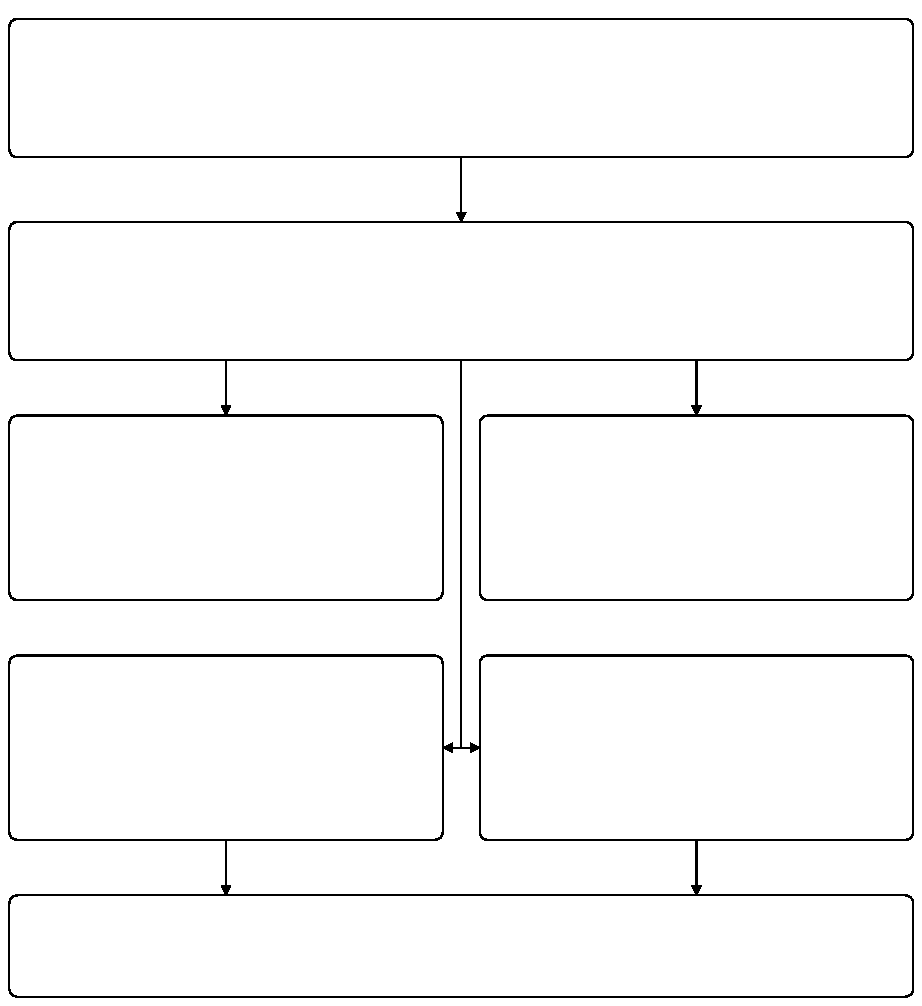
\includegraphics[width=\linewidth]{figures/rank_mechanism_geometry.pdf}}
\put(50.000,99.500){\makebox(0,0){\parbox{96.000\unitlength}{\centering\fontsize{9.4}{11.8}\selectfont Hypothetical open set: $h_1h_2h_3\ne0$\\Dense normalization chart: $\mu_1\mu_2\mu_3\ne0$}}}
\put(50.000,77.500){\makebox(0,0){\parbox{96.000\unitlength}{\centering\fontsize{9.2}{11.5}\selectfont $\rho=\operatorname{rank}d\mathsf X$ is constant\\Fibre dimension $=$ induced similarity algebra dimension $=3-\rho$}}}
\put(24.500,54.000){\makebox(0,0){\parbox{45.000\unitlength}{\centering\fontsize{9.2}{11.5}\selectfont $\rho=0$: constant abnormality ratios\\Contradiction from the frame equations}}}
\put(75.500,54.000){\makebox(0,0){\parbox{45.000\unitlength}{\centering\fontsize{9.2}{11.5}\selectfont $\rho=1$: two common generators\\Four source types force some $h_i=0$}}}
\put(24.500,28.000){\makebox(0,0){\parbox{45.000\unitlength}{\centering\fontsize{9.0}{11.2}\selectfont $\rho=2$: one common generator\\Isometry or dilation; rotation is allowed\\Each possibility is excluded}}}
\put(75.500,28.000){\makebox(0,0){\parbox{45.000\unitlength}{\centering\fontsize{8.8}{11.0}\selectfont $\rho=3$: discrete fibres\\Algebraic closure of the state image\\has dimension at most two}}}
\put(50.000,6.500){\makebox(0,0){\parbox{96.000\unitlength}{\centering\fontsize{8.9}{11.1}\selectfont $h_1h_2h_3\equiv0\ \Longrightarrow\ $a fixed $h_i\equiv0$ by analyticity\\A principal direction is normal to surfaces; Kafadar applies.}}}
\end{picture}
\caption{The four ranks of the normalized state map on a region with three nonzero abnormalities. Proposition~\ref{fnd:symmetry} identifies the fibre dimension with the dimension of the induced similarity algebra. Analyticity then selects one integrable principal plane field.}
\label{fig:rank-mechanism}
\end{figure}

\section{States of rank zero and one}\label{fnd:seclowrank}\label{sec:lowranks}

The fibres of a state of rank one are surfaces. By
Proposition~\ref{fnd:symmetry}, they are the orbits of a two dimensional
algebra of similarities common to the two flat metrics. We first
classify these algebras and then show that their orbit equations force
an integrable principal plane field. This will exclude ranks zero and
one on the domain \eqref{fnd:protected}.
In Euclidean developments, write $F_f=Df$ and
$C_f=F_f^{\top}F_f$ for the matrix of $c$.

\subsection{Two dimensional algebras of common similarities}

At a point of a rank one chart, evaluation identifies the common
similarity algebra with the tangent plane to the state fibre. Its two
generators are therefore independent after the chart is restricted.
The two Euclidean developments realize the same Lie algebra, with the
same dilation character, and the developing map intertwines their
actions.

Write $D=x\cdot\partial_x$, $R_z=-y\partial_x+x\partial_y$, and $T_z=\partial_z$. Up to a Euclidean change of coordinates and a change of generators, the list is
\begin{equation}\label{fnd:fourtypes}
\langle T_x,T_y\rangle,\qquad \langle R_z,T_z\rangle,\qquad
\langle D+\omega R_z,T_z\rangle,\qquad \langle D,R_z\rangle.
\end{equation}
The rotation projection of a two dimensional algebra has dimension at most one: two independent rotation vectors have a cross product outside their plane. If its dilation character vanishes, a nonabelian two dimensional isometry algebra would make a skew rotation act on a translation line by a nonzero real eigenvalue, which is impossible. The algebra is abelian; its rotational part is either zero, giving two translations, or one dimensional, giving a rotation and an axial translation after removing the perpendicular center and subtracting the axial translation.

If the dilation character is nonzero, its kernel is one dimensional. A kernel generator with rotational part forces commutation in the rotational projection. Center the generator with nonzero scale; its linear part is $I+\Omega$, which is invertible over the reals. A commuting kernel translation would solve $(I+\Omega)t=0$, so vanishes. This gives $\langle D,R_z\rangle$ after subtracting a rotation. A translational kernel must be a real eigenline of $I+\Omega$, hence lies on the rotation axis, giving $\langle D+\omega R_z,T_z\rangle$. The same classification applies in the second Euclidean development with the common dilation character.

For the Killing types, the target algebra is abelian and consists of
two translations or a rotation and an axial translation. When the
dilation character is nonzero, the Lie bracket distinguishes the
translation ideal from the commuting rotation ideal. The target
algebra has the corresponding type, with an independent angular rate.

\subsection{Two common Killing fields}

\begin{lemma}\label{fnd:two-killing-generators}
If a two dimensional algebra of common similarities has zero dilation
character, at least one principal abnormality vanishes on a nonempty
open subset.
\end{lemma}
\begin{proof}
There are two source orbit types in \eqref{fnd:fourtypes}.
For two translations, choose their orbit planes to be
$z=\mathrm{constant}$. The distinct principal values imply that each
labelled principal projector is translation invariant, so $P_i=P_i(z)$.
Set $q_i=(P_i)_{zz}$ and
$v_i=((P_i)_{xz},(P_i)_{yz})$. The projector pressure equations and
the orthogonality of the projectors give
\begin{equation}\label{fnd:translationprojectors}
v_i''=0,\qquad |v_i|^2=q_i(1-q_i),\qquad
-v_i\cdot v_j=q_iq_j=:C_{ij},\qquad \sum_iq_i=1.
\end{equation}
If all $q_i$ are positive, then
$q_i^2=C_{ij}C_{ik}/C_{jk}$ and
$q_i=q_i^2+C_{ij}+C_{ik}$ show that $q_i$ is rational in $z$.
The monic equation $q_i^2-q_i+|v_i|^2=0$ makes it a polynomial of
degree at most one. Its quadratic coefficient gives
$(q_i')^2+|v_i'|^2=0$. Consequently every $P_i$ is constant.
Here $P_i=(v_i,q_i)(v_i,q_i)^{\top}/q_i$.

If some $q_i$ vanishes on an interval, its principal direction lies
in an orbit plane. If two vanish, the remaining direction is axial.
Otherwise the orbit metric has one fixed relative eigenvalue
$\lambda_i$ and another eigenvalue $m$. Its flat Gauss equation gives
$(\lambda_i-m)^2(\theta')^2=0$, where $\theta$ is the
angle of the horizontal principal direction. A nonconstant $\theta$
would force $m=\lambda_i$ and a constant mixing angle for the other
two directions. Their affine off-diagonal components would then
have constant norm, and hence be constant, contrary to rotation.
Thus the horizontal principal direction is constant as well.
These alternatives exhaust an interval after restriction; in each
case some $h_i$ vanishes.

For a rotation and an axial translation, use cylindrical coordinates
$(r,\phi,z)$ with $r>0$. Write $q_i=(P_i)_{rr}$ and
$(U_i,V_i)=((P_i)_{r\phi},(P_i)_{rz})$ in the physical frame.
The projector pressure equations integrate to
\begin{equation}\label{fnd:cylinderlaurent}
U_i=\beta_{i,0}+\beta_{i,-2}/r^2,\qquad
V_i=\beta_{i,1}r+\beta_{i,-1}/r.
\end{equation}
The coefficients are real constants. If all $q_i$ are positive, the
same rational reconstruction and monic equation make them Laurent
polynomials. In $q_i^2-q_i+U_i^2+V_i^2=0$, an extreme nonzero power
in the squared terms has a positive sum of squares as coefficient.
Thus all components are constant and \eqref{fnd:cylinderlaurent}
gives $V_i=0$, which would place all three principal directions in
the radial--azimuthal plane.

If the three $q_i$ are not simultaneously positive on any
subinterval, one vanishes on a subinterval. Restrict so that each
remaining $q_j$ is either positive or identically zero, and develop
the cylindrical orbit metric into the
target Euclidean space. The target orbits are planar or cylindrical.
The planar case gives an axial principal direction. In the
cylindrical case, constant volume makes the squared target radius
affine in $r^2$. The fixed orbit eigenvalue then gives either an
axial or azimuthal principal direction, or the relation
$V_j=\kappa rU_j$ for the other two projectors. In the last
alternative, their two-plane projection identity and
\eqref{fnd:cylinderlaurent} force $U_j=V_j=0$, contrary to
$q_jq_k>0$. The orbit metric calculation, including the case in
which its two relative eigenvalues coincide, is given in
Appendix~\ref{appn:two-killing-proof}. Every remaining principal
direction found above has $h_i=0$.
\end{proof}

\subsection{Two common similarities with nonzero scale}

\begin{lemma}\label{fnd:two-similarity-generators}
If a two dimensional algebra of common similarities has nonzero
dilation character, at least one principal abnormality vanishes on
a nonempty open subset.
\end{lemma}
\begin{proof}
Consider first the nonabelian algebra
$\langle D+\omega R_z,\partial_z\rangle$.
Its translation ideal is preserved by the developing map, and its
target generators can be written as $D+\widetilde\omega R_Z$ and
$\kappa\partial_Z$, with $\kappa\ne0$. Equivariance therefore gives
\begin{equation}\label{fnd:nonabelianmap}
f(x,y,z)=(f_\perp(x,y),\kappa z+\varphi(x,y)).
\end{equation}
The planar Jacobian $J_\perp=\det Df_\perp$ is a nonzero constant.
Both $\varphi$ and
$\widetilde\varphi=\varphi\circ f_\perp^{-1}$ are harmonic.
Indeed, $\operatorname{div}C_f=F_f^{\top}\Delta f$ because the trace
is constant. Its axial component is $\kappa\Delta\varphi$,
independent of $z$, and closedness makes it constant. Equivariance
gives $(D+\omega R_z)\varphi=\varphi$, so
$[\Delta,D+\omega R_z]=2\Delta$ forces this constant to vanish.
The inverse divergence identity \eqref{fnd:inverseidentity} gives
the same conclusion for $\widetilde\varphi$ in the target plane.

If $\varphi$ is locally constant, the axial direction is principal.
Otherwise take its harmonic conjugate and use the resulting complex
potential as a local coordinate. Equivariance makes this potential
a power of $x+iy$ with exponent $(1+i\omega)^{-1}$.
The two trace constraints and constant planar Jacobian then give
\eqref{fnd:harmonicb}--\eqref{fnd:harmonicP}. For $\omega\ne0$,
equality of mixed derivatives would give a finite relation between
distinct complex exponentials with a nonzero extreme coefficient.
Their linear independence excludes this case. The identities and
coefficient comparison are derived in
Appendix~\ref{appn:nonabelian-proof}.
If $\omega=0$, the source height is affine and the target height has
constant gradient norm. Harmonicity and the Bochner identity make
the latter affine. Their constant gradients fix one row of
$Df_\perp$; its constant determinant and norm fix the other row.
Thus $f$ is affine. The nonabelian type always has some $h_i=0$.

For the abelian algebra $\langle D,R_z\rangle$, centering the target
homothety removes its translation part. A commuting target Killing
field is a nonzero rotation about the same axis. In spherical source
coordinates, the general equivariant map is
\begin{equation}\label{fnd:drmap}
f=r\bigl(U(\theta)\cos\Psi,U(\theta)\sin\Psi,V(\theta)\bigr),
\qquad \Psi=k\phi+\omega\log r+\psi(\theta),\quad U>0,
\end{equation}
where $k\ne0$. Constant volume gives
\begin{equation}\label{fnd:drvolume}
\det F_f=J=\frac{kU(U'V-UV')}{\sin\theta}\ne0.
\end{equation}
Set $x=\cos\theta$, $\mathcal N=U^2+V^2$,
$y=V/\sqrt{\mathcal N}$ and
$\widetilde{\mathcal N}(y)=1/\mathcal N(x)$.
The pressure equations for $C_f$ and $C_f^{-1}$, together with
\eqref{fnd:drvolume}, yield
\begin{equation}\label{fnd:doublelegendre}
\begin{aligned}
(1-x^2)\mathcal N''-2x\mathcal N'+6\mathcal N&=A_0,\\
y'&=(J/k)\mathcal N^{-3/2},\qquad Jk\ne0,\\
(1-y^2)\widetilde{\mathcal N}''-2y\widetilde{\mathcal N}'+6\widetilde{\mathcal N}&=B_0,
\qquad \widetilde{\mathcal N}(y(x))=\mathcal N(x)^{-1},
\end{aligned}
\end{equation}
with real constants $A_0,B_0$; the derivation is in
Appendix~\ref{appn:commuting-equations}.
Lemma~\ref{fnd:legendre} gives either a constant $\mathcal N$ or
the quadratic alternative \eqref{fnd:quadraticnorm}.
In both cases, the remaining angular pressure equation and the
constant trace reduce \eqref{fnd:drmap} to the logarithmic
cylindrical map \eqref{fnd:logcylinder}; see
Appendix~\ref{appn:phaseproof}. Its axial direction is principal,
and the other two principal directions make constant angles with
the radial direction. Their abnormalities all vanish.
\end{proof}

\begin{theorem}\label{fnd:lowrankexclusion}
A solution chart satisfying \eqref{fnd:protected} has neither state
rank zero nor state rank one.
\end{theorem}
\begin{proof}
Theorem~\ref{fnd:rankconstant} makes the state rank constant.
Rank zero makes $\widehat h_2,\widehat h_3$ constant, contrary to
Lemma~\ref{fnd:constantratio}. At rank one,
Proposition~\ref{fnd:symmetry} gives a two dimensional common
similarity algebra. The list \eqref{fnd:fourtypes} is exhausted by
Lemmas~\ref{fnd:two-killing-generators} and
\ref{fnd:two-similarity-generators}, both of which contradict
$h_1h_2h_3\ne0$.
\end{proof}

Thus a positive dimensional state fibre on \eqref{fnd:protected}
has dimension one, and its symmetry algebra is generated by a single
common similarity. The next three sections exclude this rank two
case.

\section{Similarity reduction}\label{sec:similarity}

At rank two, the state fibres are the orbits of one common
similarity. Its Euclidean representations determine the deformation
along each orbit, leaving data on a transverse surface. We derive
the equations for these data and the normal forms used in
Sections~\ref{sec:isometries} and~\ref{sec:dilation}.

\subsection{The common generator}

\begin{proposition}[One common similarity]\label{sim:generator}
If $\operatorname{rank}d\mathsf X=2$, there is locally a one
dimensional Lie algebra of vector fields $Z$ satisfying
\begin{equation}\label{sim:commutation}
[Z,E_i]=0,\qquad Z\mathsf X=0.
\end{equation}
Evaluation identifies this algebra with $\ker d\mathsf X$.
A nonzero generator is nowhere zero on a sufficiently small chart
and is a homothety of both metrics with the same constant factor.
\end{proposition}
\begin{proof}
Apply Proposition~\ref{fnd:symmetry} with $\rho=2$.
The evaluation isomorphism makes a nonzero generator nowhere zero
after restriction. If $k=Z\log|h_1|$, the common homothety equations
are
\begin{equation}\label{sim:equalmetricfactor}
\mathcal L_Zg=-2kg,\qquad \mathcal L_Zc=-2kc.
\end{equation}
Thus the two homothety factors agree.
\end{proof}

In the two Euclidean developments, the representations $Z_s,Z_t$
are intertwined by $f$:
\begin{equation}\label{sim:intertwine}
Df(x)Z_s(x)=Z_t(f(x)).
\end{equation}
Differentiating the Euclidean homothety equation
$\partial_iZ_j+\partial_jZ_i=2\sigma\delta_{ij}$ and taking cyclic
permutations gives $\partial_i\partial_jZ_k=0$. Hence
\begin{equation}\label{sim:affine}
\begin{gathered}
Z_s(x)=\sigma_sx+\Omega_sx+t_s,\qquad
Z_t(y)=\sigma_ty+\Omega_ty+t_t,\\
\Omega_s^{\top}=-\Omega_s,\qquad \Omega_t^{\top}=-\Omega_t.
\end{gathered}
\end{equation}
The fixed trace gives
\begin{equation}\label{sim:tracefactor}
0=Z\operatorname{tr}(g^{-1}C_f)
=2(\sigma_t-\sigma_s)\operatorname{tr}(g^{-1}C_f),
\end{equation}
so $\sigma_s=\sigma_t$. The common orbit parameter therefore fixes
the relative speeds of the two affine fields.

For the transverse equations, write the fixed invariants as
\[
\mathcal I_1=\operatorname{tr}C_f,\qquad
\mathcal I_2=\operatorname{tr}\operatorname{adj}C_f,\qquad
J=\det Df.
\]
In physical incompressible coordinates
$(\mathcal I_1,\mathcal I_2,J)=(I_2,I_1,1)$.
A constant metric normalization may give a different nonzero
signed Jacobian $J$ in a developing chart.

\subsection{Equilibrium under inversion}

Exchanging the Euclidean developments replaces $f$ by its inverse
and the principal values by their reciprocals. The following lemma
shows that the same interchange preserves the hypotheses of the
classification.

\begin{lemma}[Local inverse equivalence]\label{sim:inverse}
Let $f$ be a local diffeomorphism whose matrix $C_f$ has constant,
positive, pairwise distinct principal values. The closedness
conditions
\begin{equation}\label{sim:two-pressures}
d(\operatorname{div}C_f)^\flat=0,\qquad
d(\operatorname{div}C_f^{-1})^\flat=0
\end{equation}
hold if and only if they hold for $f^{-1}$. Each labelled projector
pressure is transported as the same scalar function, and each
labelled principal abnormality has the same zero set in the two
configurations.
\end{lemma}
\begin{proof}
Put $F_{f^{-1}}=D(f^{-1})$ and
$\overline{C_f}=F_{f^{-1}}^{\top}F_{f^{-1}}$.
Since the traces and Jacobian are constant, differentiation gives
\begin{equation}\label{sim:divergence-identities}
\begin{aligned}
\operatorname{div}_xC_f&=F_f^{\top}\Delta_xf,\\
\operatorname{div}_xC_f^{-1}&=(\Delta_yf^{-1})\circ f,\\
\operatorname{div}_y\overline{C_f}
&=F_{f^{-1}}^{\top}\Delta_yf^{-1},\\
\operatorname{div}_y\overline{C_f}^{-1}
&=(\Delta_xf)\circ f^{-1}.
\end{aligned}
\end{equation}
The first identity follows by differentiating
$(C_f)_{ij}=\sum_a(F_f)_{ai}(F_f)_{aj}$ and commuting mixed
derivatives. For the second, write
$(C_f^{-1})_{ij}=\sum_a(F_{f^{-1}})_{ia}(F_{f^{-1}})_{ja}$
at $f(x)$ and use the chain rule. Differentiation of the two
factors gives $\Delta_y(f^{-1})_i$ and
$-(C_f^{-1}\nabla_x\log|J|)_i$, respectively; the latter vanishes.
The last two identities follow by interchanging $f$ and $f^{-1}$.

On a simply connected chart, choose pressure potentials
$\operatorname{div}C_f=\nabla p_{C_f}$ and
$\operatorname{div}C_f^{-1}=\nabla p_{C_f^{-1}}$.
Equation~\eqref{sim:divergence-identities} yields
\begin{equation}\label{sim:inversepressures}
\operatorname{div}_y\overline{C_f}
=\nabla_y(p_{C_f^{-1}}\circ f^{-1}),\qquad
\operatorname{div}_y\overline{C_f}^{-1}
=\nabla_y(p_{C_f}\circ f^{-1}).
\end{equation}
The same argument applied to the inverse proves equivalence.

Write $C_f=\sum_i\lambda_iP_i$ and
$\operatorname{div}P_i=\nabla\phi_i$, with $\sum_i\phi_i=0$.
The inverse projectors $\overline P_i$ have principal values
$\lambda_i^{-1}$. The coefficient matrix with rows
$(1,1,1)$, $(\lambda_1,\lambda_2,\lambda_3)$ and
$(\lambda_1^{-1},\lambda_2^{-1},\lambda_3^{-1})$ is invertible.
Thus \eqref{sim:inversepressures} and
$\operatorname{div}\sum_i\overline P_i=0$ imply
\begin{equation}\label{sim:labelpressures}
\operatorname{div}_y\overline P_i
=\nabla_y(\phi_i\circ f^{-1}).
\end{equation}
For unit principal vectors, put
$\overline e_i=F_fe_i/\sqrt{\lambda_i}$.
Then $f^*\overline\alpha_i=\sqrt{\lambda_i}\alpha_i$, and hence
\begin{equation}\label{sim:contacttransform}
f^*(\overline\alpha_i\wedge d\overline\alpha_i)
=\lambda_i\alpha_i\wedge d\alpha_i,
\qquad
\overline h_i\circ f=\frac{\lambda_i}{J}h_i.
\end{equation}
This preserves the zero sets for either sign of $J$.
\end{proof}

\subsection{Normal forms of the generator pair}

When the common scale is zero, each generator is a Euclidean
Killing field. In cylindrical coordinates, its three normal forms
are
\begin{equation}\label{sim:killingtypes}
\begin{array}{lll}
\mathrm T&\text{translation}:&p\,\partial_z,\quad p\ne0,\\
\mathrm R&\text{rotation}:&\omega\,\partial_\theta,\quad\omega\ne0,\\
\mathrm S&\text{screw motion}:&\omega\,\partial_\theta+p\,\partial_z,
\quad\omega p\ne0.
\end{array}
\end{equation}
A pair lists the source generator first and the target generator
second. Lemma~\ref{sim:inverse} permits their interchange.

\begin{proposition}[Normal forms of one generator]\label{sim:types}
Up to separate fixed Euclidean coordinate changes and a common
nonzero rescaling of $Z$, a rank two chart has either one of the
six Killing pairs
\begin{equation}\label{intro:sixpairs}
(\mathrm T,\mathrm T),\quad(\mathrm T,\mathrm R),\quad
(\mathrm T,\mathrm S),\quad(\mathrm R,\mathrm R),\quad
(\mathrm R,\mathrm S),\quad(\mathrm S,\mathrm S),
\end{equation}
or a pair with nonzero common scale
\begin{equation}\label{sim:dilationpair}
(D+\omega_sR,\ D'+\omega_tR'),\qquad
\omega_s,\omega_t\in\mathbb R.
\end{equation}
Here $D=x\cdot\partial_x$, $D'=y\cdot\partial_y$,
$R=\partial_\theta$ and $R'=\partial_\Theta$.
The two angular rates may vanish independently. The speeds and
screw pitches are subject to the intertwining identity
\eqref{sim:intertwine}.
\end{proposition}
\begin{proof}
For a Killing field with nonzero rotational part, decompose the
translation into axial and perpendicular components. The skew map
is invertible on the perpendicular plane, so shifting the axis
removes the perpendicular component. The remaining axial component
gives a rotation or a screw motion; a zero rotational part gives a
translation. Both generators are nonzero because $Df$ is invertible.
Inversion reduces their ordered pairs to \eqref{intro:sixpairs}.

If $\sigma\ne0$, the matrix $\sigma I+\Omega$ is invertible over
the reals. A unique change of origin removes the translation.
Rescaling the common generator by $\sigma^{-1}$ and aligning the
axes gives \eqref{sim:dilationpair}.
\end{proof}

\begin{table}[htbp]
\centering
\small
\renewcommand{\arraystretch}{1.12}
\setlength{\tabcolsep}{3pt}
\caption{The six Killing pairs on the branch $h_1h_2h_3\ne0$.
For the two cylindrical alternatives, all principal abnormalities vanish.}
\label{tab:killing-pairs}
\begin{tabular}{@{}>{\raggedright\arraybackslash}p{0.13\linewidth}>{\raggedright\arraybackslash}p{0.37\linewidth}>{\raggedright\arraybackslash}p{0.18\linewidth}>{\raggedright\arraybackslash}p{0.27\linewidth}@{}}
\toprule
Pair & Argument & Consequence & Proof location\\
\midrule
$(\mathrm T,\mathrm T)$ &
Finite Hessian choices on transverse slices &
$\rho\le1$ &
Lemmas~\ref{iso:finite-fibres} and~\ref{iso:tt-fibres}\\
\addlinespace
$(\mathrm T,\mathrm R)$ &
Algebraic reconstruction and finite transverse fibres &
$\rho\le1$ &
Lemmas~\ref{iso:finite-fibres} and~\ref{iso:trs-fibres}\\
\addlinespace
$(\mathrm T,\mathrm S)$ &
Algebraic reconstruction and finite transverse fibres &
$\rho\le1$ &
Lemmas~\ref{iso:finite-fibres} and~\ref{iso:trs-fibres}\\
\addlinespace
$(\mathrm R,\mathrm R)$ &
Compact continuation and local dimension bounds &
Cylindrical;\newline $h_i=0$ &
Sections~\ref{iso:two-rotations} and~\ref{iso:rotation-fibres}\\
\addlinespace
$(\mathrm R,\mathrm S)$ &
Continuation and the Killing field norm estimate &
No solution germ &
Equation~\eqref{iso:rotation-screw-bound} and Lemma~\ref{iso:continuation}\\
\addlinespace
$(\mathrm S,\mathrm S)$ &
Radial limits and the pitch relation &
Cylindrical;\newline $h_i=0$ &
Section~\ref{iso:two-screws}\\
\bottomrule
\end{tabular}
\end{table}

The common parameter fixes the relative speeds, but does not equate
the angular rates. For the logarithmic cylindrical map
\eqref{fnd:logcylinder},
$f_*(D+\omega_sR)=D'+(\omega+k\omega_s)R'$.
All angular coordinates below are local lifts.

\subsection{Equations on a transverse surface}

Let $\Phi_s^t,\Phi_t^t$ be the affine flows, and choose a source
surface $x_0(u,v)$ transverse to $Z_s$. Equivariance is equivalent to
\begin{equation}\label{sim:flowmap}
f(\Phi_s^t x_0(u,v))=\Phi_t^t y_0(u,v).
\end{equation}
Indeed, both sides solve the target orbit equation with the same
initial value. Conversely, any surface $y_0$ for which the resulting
map is a local diffeomorphism defines an equivariant map.
At $t=0$, its derivative is determined by
\begin{equation}\label{sim:surfacegrad}
F_{f,0}[Z_s(x_0),\partial_ux_0,\partial_vx_0]
=[Z_t(y_0),\partial_uy_0,\partial_vy_0].
\end{equation}
The equal scale factors cancel along the flows, so
\begin{equation}\label{sim:gradientflow}
Df(\Phi_s^t x_0)=e^{t\Omega_t}F_{f,0}e^{-t\Omega_s}.
\end{equation}
Consequently constant principal values are equivalent to the
three constraints on the transverse surface
\begin{equation}\label{sim:surfaceinvariants}
\operatorname{tr}(F_{f,0}^{\top}F_{f,0})=\mathcal I_1,\qquad
\operatorname{tr}\operatorname{adj}(F_{f,0}^{\top}F_{f,0})=\mathcal I_2,
\qquad\det F_{f,0}=J.
\end{equation}
Flatness follows from the representation \eqref{sim:flowmap}.

For equilibrium, let $M$ be the covariant tensor associated with
$g^{-1}c$ or its inverse; in Euclidean coordinates its matrix is
$C_f$ or $C_f^{-1}$. A constant homothety preserves the connection.
The homothety weights of $M$ and of the inverse metric in its
divergence cancel, giving
\begin{equation}\label{sim:pressureinvariance}
\mathcal L_Z\bigl((\operatorname{div}_gM)^\flat\bigr)=0.
\end{equation}
In flow coordinates, write this invariant one-form as
\[
(\operatorname{div}_gM)^\flat
=a_t(u,v)\,dt+a_u(u,v)\,du+a_v(u,v)\,dv.
\]
Closedness is equivalent to
\begin{equation}\label{sim:pressurePDE}
\partial_ua_t=0,\qquad\partial_va_t=0,\qquad
\partial_ua_v-\partial_va_u=0.
\end{equation}
On a small connected transverse disk, the pressure therefore has
the form
\begin{equation}\label{sim:pressurepotentials}
p_M(t,u,v)=K_Mt+\psi_M(u,v)+\hbox{constant},
\end{equation}
where $K_M$ is a real constant. There is one such system for each
of the two tensors. For individual projectors, the same argument gives
\begin{equation}\label{sim:projectorpressureconstants}
Z\phi_i=K_i,\qquad\sum_iK_i=0.
\end{equation}
Equation~\eqref{sim:labelpressures} transports these constants to the
inverse configuration.

Thus \eqref{sim:surfaceinvariants} and \eqref{sim:pressurePDE}
give the kinematic and equilibrium equations on the transverse
surface. The next section treats the Killing pairs; Section~\ref{sec:dilation}
treats \eqref{sim:dilationpair}.

\section{Common Euclidean isometries}\label{iso:section}\label{sec:isometries}

We now consider the pairs of common Euclidean isometries in
Section~\ref{sec:similarity}. Throughout, rank means the rank of
$\mathsf X$ in \eqref{fnd:X}, and $C_f,\mathcal I_1,\mathcal I_2,J$
have the meaning fixed there. We also write $j=\det C_f=J^2>0$.
The constant principal values $\lambda_i$ are positive and pairwise
distinct. The universal deformation equations are
\begin{equation}\label{iso:universal}
 \operatorname{curl}\operatorname{div}C_f=0,\qquad
 \operatorname{curl}\operatorname{div}C_f^{-1}=0.
\end{equation}
The pressures are local potentials. When an angular coordinate is used,
we lift it to a real coordinate on the universal cover of the complement
of the axis. The matrices $\Omega_s,\Omega_t$ retain the meaning in
\eqref{sim:affine}. Their axial vectors are defined by
$\Omega_sx=\Omega_s^{\rm axial}\times x$ and
$\Omega_ty=\Omega_t^{\rm axial}\times y$; in principal components they
are expressed in the corresponding principal frames.

A common Killing field makes the state constant along its orbits.
The two transverse variables can still carry a state of rank two;
the problem is therefore to constrain this transverse dependence.
For pairs containing a translation, the orbit equations leave one
scalar parameter with finite reconstruction fibres. For rotating
sources, the natural length is the distance from the axis. Bounding
the state at this scale permits continuation and radial limits. The
two-rotation problem then becomes a dimension comparison on a compact
state set, while the normalized pitches of two screw motions tend to
zero at large radius.

\begin{theorem}[Exclusion of a common isometry at rank two]\label{iso:theorem}
For every triple of positive, pairwise distinct, constant principal values of the strain tensor, no
rank two state arising from a solution on an open set where $h_1h_2h_3\ne0$ admits a nonzero
common Euclidean Killing field.  
\end{theorem}

\subsection{Reconstruction and continuation}

Continuation and radial limits require a state set closed under
limits of the frame coefficients. We therefore include the common
Killing field, its angular data and the longitudinal pressure data in
the state of Section~\ref{sec:geometry}. Differentiating their algebraic
constraints gives an invariant closed set on which the same
reconstruction applies.

We use $\mathsf S$ and the fields $\mathcal Q_i$ from
\eqref{fnd:17state} and \eqref{fnd:weighted-state}.
Write $w_i^Z=\alpha_i(Z_s)$ for the principal components of the common
Killing field. The augmented derivations $B_i$ are defined on these
coordinates by the first two relations below. The third relation
is the algebraic constraint that the state is constant along the common orbit:
\begin{equation}\label{iso:raw-killing}
 B_i\mathsf S=\mathcal Q_i(\mathsf S),\qquad B_iw_l^Z=\sum_k w_k^ZC^l_{ki}(\mathsf S),\qquad
 \sum_i w_i^Z\mathcal Q_i(\mathsf S)=0.
\end{equation}
Their coefficients have only the fixed spectral denominators.

\begin{definition}[State with fixed isometry data]\label{iso:complete-state}
Let $\mathsf U$ consist of $\mathsf S$, the principal components of the
common Killing field, and the source and target angular vectors.
Transporting the latter by the two metric connections extends
\eqref{iso:raw-killing} to polynomial derivations $B_i$ of
$\mathbb R[\mathsf U]$. The principal values and isometry data
are fixed, so every spectral denominator is a nonzero constant.

Let $\mathscr J_0$ be the ideal of the original compatibility and bracket
equations, the orbit relation in \eqref{iso:raw-killing}, and the equations
identifying the angular vectors, their prescribed norms and pitches,
and the derivatives of the pressure potentials along the common orbit.
The angular and pressure equations are written explicitly in
\eqref{appiso:angular-observations} and \eqref{dil:pressure-matrix},
with the physical target angular vector obtained by the metric
conversion specified there.
Define
\begin{equation}\label{iso:differential-ideal}
 \mathscr J=\left\langle
 B_{i_1}\cdots B_{i_m}q:
 q\in\mathscr J_0,\ m\ge0,\ i_\ell\in\{1,2,3\}
 \right\rangle\subset\mathbb R[\mathsf U].
\end{equation}

Write $\mathscr N$ for its real zero set, with a subscript specifying
the isometry pair. Fix source and target frames and base values to
remove the development constants, including the constant target phase
and axial translation when the target is axial.
\end{definition}

Noetherianity of $\mathbb R[\mathsf U]$ gives finitely many generators of $\mathscr J$.
Thus $\mathscr N$ is a closed real algebraic set and is invariant under the
ambient polynomial state flows wherever they are defined.
The augmented bracket identity is
\begin{equation}\label{iso:augmented-bracket}
 \left([B_i,B_j]-\sum_kC^k_{ij}B_k\right)w_l^Z
      =\sum_k w_k^Z\mathcal Q_k(C^l_{ij})=0,
\end{equation}
where the last equality is the weight one part of
\eqref{iso:raw-killing}.

\begin{lemma}[Reconstruction with fixed isometry data]
\label{iso:augmented-reconstruction}
The state set in Definition~\ref{iso:complete-state} has local
realizations satisfying the prescribed common isometry and pressure
equations. After the development constants are fixed, the kernel
of the differential of its defining ideal identifies with the space of
formal linearized germs with the same fixed data.
\end{lemma}
\begin{proof}
Lift the augmented fields to the source orthonormal frame bundle.
The displayed bracket identity, torsion and Euclidean flatness make
their Cartesian combinations commute. Their flows reconstruct the
first metric, and development of the second flat metric reconstructs
$f$, as in Proposition~\ref{fnd:reconstruction}. The appended equations
reconstruct a common Killing field; its value and covariant derivative
determine its Euclidean translation and angular parts. The fixed
data therefore impose the prescribed isometry pair.
The closed pressure forms reconstruct the local potentials.

The same calculation over $\mathbb R[\epsilon]/(\epsilon^2)$
includes the appended equations and all their derivatives.
The commuting Cartesian flows and their variational equations
reconstruct a formal linearized germ of the full equivariance system.
The converse follows by differentiating that system.
This is Lemma~\ref{fnd:linearized-reconstruction} applied to the augmented system.
\end{proof}

The connection and its two retained jets have weights one, two and
three. Multiplication by the corresponding powers of $\mu=|Z_s|$
removes their physical length scale. The angular equations constrain
these dimensionless quantities when the common field is transverse
to the rotation axis.

\begin{lemma}[Transverse compactness]\label{iso:compactness}
Fix positive, pairwise distinct principal values, bounded angular data,
and bounded longitudinal pressure data.  Put $\mu=|Z_s|$,
$\nu=Z_s/\mu$.  If the source angular vector $\Omega_s^{\rm axial}$ satisfies
$|\Omega_s^{\rm axial}\times\nu|\ge d>0$, then
\[
 (\mu\boldsymbol p,\mu^2\boldsymbol\tau,\mu^3\boldsymbol u,\nu)
\]
is bounded on the augmented real state set.  
\end{lemma}
\begin{proof}
Suppose an unbounded sequence satisfies the bounds on the data and the
stated transversality. The common-field and compatibility equations give
\begin{equation}\label{iso:compactness-jet-bounds}
 |\mu^2\boldsymbol\tau|\le C(1+|\mu\boldsymbol p|)^2,
 \qquad
 |\mu^3\boldsymbol u|\le C(1+|\mu\boldsymbol p|)^3.
\end{equation}
Hence, after passing to a subsequence, $|\mu\boldsymbol p|\to\infty$.
The unit directions and bounded data have limits. Normalize by
the inverse size $\varepsilon$ of these frame coefficients. Away from
principal directions the angular data leave at most one
homogeneous connection direction; a nonzero quadratic compatibility
equation excludes it. This also covers directions with just one zero
principal component.

At a principal direction the homogeneous limit is the plane
\eqref{iso:escape-plane}. If the normal distance to this plane is
$O(|\varepsilon|)$, the first-order angular forcing in the unprojected
equations cannot be cancelled by their quadratic remainder. Its source
components are nonzero by transversality, giving a contradiction.

If the normal distance divided by $|\varepsilon|$ tends to infinity,
the quadratic normal equations apply.
At either extreme principal direction their first form is definite.
At the middle direction it has two null lines. Along either line,
the next orders first determine the moving normal centre and then give
a strictly positive fourth-order remainder. When the coefficient
determining that centre tends to zero, the equivalent system in the
derived normal variables gives incompatible limits for its quadratic
and linear components. The two projective endpoints are treated in the charts where their
nonzero connection coordinate is normalized to one. The normal
equations and their fourth-order terms are written in
Appendix~\ref{appiso-compactness}. After passage to a subsequence, the
ratio of the normal distance to $|\varepsilon|$ is bounded or tends to
infinity. The first case contradicts the angular forcing; the second
contradicts the normal equations just described.
\end{proof}

\begin{lemma}[Continuation away from the axis]\label{iso:continuation}
A solution germ with a rotating source satisfying the augmented equations extends
along every finite path in the complement of its source axis. It therefore extends to the
universal cover of that complement.
\end{lemma}
\begin{proof}
Write $Z_s=\omega e_z\times x+pe_z$.  On an off-axis compact set,
\[
 |Z_s|^2=\omega^2r^2+p^2,\qquad
 |\Omega_s^{\rm axial}\times Z_s|/|Z_s|
 =\omega^2r/(\omega^2r^2+p^2)^{1/2}>0
\]
uniformly.  Lemma~\ref{iso:compactness} bounds all unnormalized states there.
Along a finite path integrate \eqref{iso:raw-killing}, both frame
connections, and
\[
 df=\overline{\mathbf E}\operatorname{diag}(\sqrt{\lambda_i})\mathbf E^{\top}\,dx.
\]
Frames remain in compact orthogonal groups and $f$ remains bounded by the
fixed largest singular value times path length.  The analytic right-hand
sides have only the positive principal values and their differences.  A finite first
obstruction therefore has a Cauchy limit and the ODE extends through it.
The differential ideal is preserved, and reconstruction realizes
every continued state as a local germ.
\end{proof}

Continuation immediately excludes a source rotation paired with a
target screw motion. Keep the common flow parameter and write
\[
 Z_s=\omega_s e_z\times x,\qquad
 Z_t=\omega_t e_Z\times y+pe_Z,
 \qquad \omega_s\omega_tp\ne0.
\]
Let $M=\sqrt{\lambda_{\max}}$.  Equivariance gives at every point
\begin{equation}\label{iso:rotation-screw-bound}
 |p|\le |Z_t(f(x))|=|DfZ_s|\le M|\omega_s|r.
\end{equation}
Hence $r\ge r_*:=|p|/(M|\omega_s|)>0$.
Starting at any germ, continue along a fixed radial segment to $r_*/2$.
This finite segment is entirely off axis, so
Lemma~\ref{iso:continuation} applies. At its endpoint, \eqref{iso:rotation-screw-bound}
would give $|p|\le|p|/2$.  Thus a rotation cannot be paired with a screw motion, even off the
region where $h_1h_2h_3\ne0$.  

\subsection{Pairs containing a translation}

For the three pairs with a translating source, the equivariant map
leaves a scalar coordinate transverse to the common orbits.  We shall
prove that the remaining reconstruction data have finite fibres over
that coordinate. The following lemmas connect this algebraic property
to the rank of the differential state and provide a criterion for
finiteness of an algebraic projection.

\begin{lemma}[Finite fibres and state rank]\label{iso:finite-fibres}
Let $v$ be a local coordinate on a solution chart.  Suppose that, for
each fixed $v$ outside a finite set, all remaining scalar reconstruction
variables take values in finite algebraic sets.  Suppose the matrices
of both metrics in an adapted orthonormal frame $(\widetilde e_i)$, that frame's
connection coefficients, and the derivatives $\widetilde D_i v$ are reconstructed
from these variables and $v$, where $\widetilde D_i=\widetilde e_i\cdot\nabla$.
Then the state of their principal frame has rank at most one.
\end{lemma}
\begin{proof}
Shrink to coordinates $(v,w,z)$ avoiding the finite exceptional levels.
On a connected $(w,z)$-slice, each reconstruction variable is continuous
and has finite image, hence is constant.  Its dependence on $v$ is smooth,
as follows by restriction to a fixed transverse section.  
The distinct principal values allow the eigenframe to be chosen smoothly as a
function of the reconstructed matrix.  The adapted connection and $\widetilde D_i v$
depend only on $v$ by hypothesis.  For any scalar $a(v)$ its frame derivative
is $a'(v)\widetilde D_i v$, again a function of $v$.  This closes the induction for the
eigenframe connection and all successive frame derivatives.  The normalized
invariant state therefore depends only on $v$.
\end{proof}

\begin{lemma}[Projection to an affine line]\label{iso:algebraic-fibres}
Let $V$ be a constructible complex algebraic set and $b$ a regular function
on it.  If no algebraic curve $\mathscr C\subset\overline V$ with $\mathscr C\cap V$ dense
in $\mathscr C$ has a place with $b=\infty$, then $b(V)$ is finite.
\end{lemma}
\begin{proof}
An infinite constructible subset of the affine line contains a nonempty
Zariski open set.  A component dominating that line contains an algebraic
curve on which $b$ is nonconstant.  On its smooth projective normalization,
the resulting nonconstant rational function has a pole.  A local
uniformizer gives a Puiseux branch with a pole.  
\end{proof}

We first consider two translations.

In Cartesian coordinates, the equivariant map is
\begin{equation}\label{iso:tt-map}
 f(x,y,z)=(f_\perp(x,y),\kappa z+\upsilon(x,y)),\qquad \kappa\ne0.
\end{equation}
Put $G=(Df_\perp)^{\top}Df_\perp$, $d_0=\det G>0$, $K=\kappa^2$, and
$v=\nabla\upsilon$.  The constant full determinant makes $d_0$ constant.  In
the source splitting,
\begin{equation}\label{iso:tt-block}
 C_f=\begin{pmatrix}G+vv^{\top}&\kappa v\\ \kappa v^{\top}&K\end{pmatrix},
 \quad
 C_f^{-1}=\begin{pmatrix}
 G^{-1}&-G^{-1}v/\kappa\\
 -v^{\top}G^{-1}/\kappa&(1+v^{\top}G^{-1}v)/K
 \end{pmatrix}.
\end{equation}
The axial components of \eqref{iso:universal} and then its planar component
give, for arbitrary real constants $P,Q$,
\begin{equation}\label{iso:tt-pdes}
 \Delta\upsilon=P,\qquad
 \operatorname{div}(G^{-1}\nabla\upsilon)=Q,\qquad
 \operatorname{curl}\operatorname{div}G=0.
\end{equation}
Indeed $\operatorname{div}(vv^{\top})=\nabla(|v|^2/2)+P\nabla\upsilon$ is a
gradient.  The two trace conditions imply, for constants $E,d$,
\[
 \operatorname{tr}G=E-|v|^2,\quad
 v^{\top}G^{-1}v=(K|v|^2+d)/d_0.
\]
On $\tau=|v|>0$ take $n=v/\tau$ and its oriented quarter-turn $t$.
The metric reconstruction is
\begin{equation}\label{iso:tt-reconstruction}
 G=\begin{pmatrix}A&G_{nt}\\G_{nt}&C_0\end{pmatrix}_{n,t},\quad
 C_0=K+d/\tau^2,\quad A=E-\tau^2-C_0,
 \quad G_{nt}^2=AC_0-d_0.
\end{equation}
Here $G_{nt}$ may have either sign.

If $v=0$ on an open set, the fixed axial direction is principal and its
corresponding $h_i$ is zero.  If $\tau$ is a positive constant, the Bochner
identity gives
\[
 0=\Delta|\nabla\upsilon|^2=2|D^2\upsilon|^2,
\]
so $\upsilon$ is affine and \eqref{iso:tt-reconstruction} makes $G$ constant.
The principal frame is consequently constant, giving $h_i=0$.
Otherwise restrict to $d\tau\ne0$.  The rational function $G_{nt}^2$ has leading
term $-K\tau^2$ at infinity and is not identically zero.  Its finitely many
zero levels therefore cannot contain a solution coordinate patch;
on a smaller chart $G_{nt}\ne0$.

\begin{lemma}[Translation fibres]\label{iso:tt-fibres}
At each fixed positive value of $\tau$, apart from finitely many levels,
the Hessian $D^2\upsilon$ takes at most two values in the frame $(n,t)$.
This holds for every real $P,Q$ and for both reconstruction signs.
\end{lemma}
\begin{proof}
The second equation in \eqref{iso:tt-pdes} places the two independent
Hessian entries on an affine line. Its two derivatives determine the
third derivatives through a matrix with strictly positive determinant,
including when $d=0$. Substitution in the remaining planar equation
gives a quadratic polynomial on that line. In the normalization of
Appendix~\ref{appiso-tt}, its leading coefficient is a nonzero rational
function of $\tau$, for every pressure pair and either reconstruction
sign. It vanishes at only finitely many levels, which proves the claim.
\end{proof}

Lemma~\ref{iso:tt-fibres} supplies the finite Hessian choices needed in
Lemma~\ref{iso:finite-fibres}; the metric reconstruction already supplies
the finite choices of $G_{nt}$.  Write $a_H=D^2\upsilon(n,n)$ and
$b_H=D^2\upsilon(n,t)$, the Hessian entries used in
Appendix~\ref{appiso-tt}.  In the frame $(n,t,e_z)$,
\[
 \begin{aligned}
 C_f&=\begin{pmatrix}A+\tau^2&G_{nt}&\kappa\tau\\G_{nt}&C_0&0\\
 \kappa\tau&0&K\end{pmatrix},\\
 \nabla_n n&=(b_H/\tau)t,\quad
 \nabla_t n=((P-a_H)/\tau)t,\quad \nabla_{e_z}n=0.
 \end{aligned}
\]
The Hessian entries also give $n\tau=a_H$, $t\tau=b_H$ and $e_z\tau=0$.
Thus both the adapted connection and the frame derivatives of the
coordinate $\tau$ are reconstructed from the same finite data.
On each connected fixed-$\tau$ slice those data are constant, so
Lemma~\ref{iso:finite-fibres} shows that the state of the principal frame
has rank at most one, contradicting Theorem~\ref{fnd:lowrankexclusion}.

For a translation paired with a rotation or screw motion, the target
angular speed is nonzero.

Write the common generators as $Z_s=a\partial_z$ and
$Z_t=\omega\partial_\Theta+b\partial_Z$, with $a\omega\ne0$.
Divide both generators by $\omega$ and use the common length scale
$|a/\omega|$ in the source and target. After choosing the source axis
orientation, the generators become $\partial_z$ and
$\partial_\Theta+p\partial_Z$. These common spatial scalings and rigid
coordinate changes preserve the singular values of $Df$. The equivariant map is
\begin{equation}\label{iso:trs-map}
 f=(R\cos(z+\psi),R\sin(z+\psi),pz+z_f),
\end{equation}
where $p$ is any real number.  Thus $p=0$ pairs the source translation with a target rotation,
and $p\ne0$ pairs it with a target screw motion.  The open image of a deformation cannot lie in the target axis.  On an off-axis
patch put
\[
 q=R^2/2,\quad \upsilon=z_f-p\psi,\quad v=2q+p^2,\quad Q=v-p^2>0.
\]
The Jacobian identity $\det Df=-\operatorname{Jac}(q,\upsilon)$ makes
$(q,\upsilon)$ local coordinates in the source plane.  If $G$ is the Euclidean
plane metric in these coordinates, then
\begin{equation}\label{iso:trs-metrics}
 \begin{aligned}
 g&=G+dz^2,\quad C_f=K+v(dz+a)^2,\\
 K&=\operatorname{diag}(Q^{-1},Q/v),\\
 a&=d\psi+(p/v)d\upsilon,\quad \det G=j^{-1}.
 \end{aligned}
\end{equation}
The equilibrium and spectral equations are
\begin{align}
 \operatorname{tr}[G^{-1}(K+vaa^{\top})]&=\mathcal I_1-v,\nonumber\\
 \operatorname{tr}(GK^{-1})&=\mathcal I_2/j-(1+va^{\top}K^{-1}a)/v,
 \label{iso:trs-traces}\\
 \operatorname{div}(vG^{-1}a)&=K_{C_f},\nonumber\\
 -\operatorname{div}(K^{-1}a)&=K_{C_f^{-1}},\label{iso:trs-vertical}\\
 d\operatorname{div}_G(K+vaa^{\top})&=0,\nonumber\\
 d\operatorname{div}_G(vK)&=0.\label{iso:trs-horizontal}
\end{align}
Here $K_{C_f},K_{C_f^{-1}}\in\mathbb R$.

\begin{lemma}[A harmonic axial coordinate]\label{iso:harmonic}
Every deformation satisfying \eqref{iso:trs-traces}--\eqref{iso:trs-horizontal}
satisfies $\Delta_Gz_f=0$.
\end{lemma}
\begin{proof}
The product rule, phase closedness, and the forward vertical equation give
\[
 \operatorname{div}_G(vaa^{\top})
 =K_{C_f}a+\frac v2d(a^{\top}G^{-1}a)+v\iota_{a^\sharp}da.
\]
Subtracting $v^{-1}\operatorname{div}_G(vK)$ and using the first trace
equation yields
\[
 \bigl(d\operatorname{div}_G(K+vaa^{\top})
       -v^{-1}d\operatorname{div}_G(vK)\bigr)_{q\upsilon}
 =-\frac4v\Delta_Gz_f.
\]
Here $dz_f=pa+K_{22}d\upsilon$ and $\det G$ is constant.
The full product identity is \eqref{appiso-harmonic-offshell}.
Both horizontal equations vanish, so $z_f$ is harmonic.
\end{proof}

The two trace equations reconstruct $G$ algebraically from $(q,a)$. Set $b=\sqrt v K^{-1/2}a$, $\mathcal N_b=b^{\top}b$ and
$\widehat G=K^{-1/2}GK^{-1/2}$.  The trace and determinant of $\widehat G$
are fixed functions of $(v,\mathcal N_b)$ and its entry in the $b$ direction is fixed
as well; its off-diagonal entry has two signs.  If $a=0$ on an open set,
the vertical direction is principal.  If that off-diagonal entry vanishes
on an open set, the horizontal direction perpendicular to $a$ is
principal.  In either case the corresponding $h_i$ vanishes:
a horizontal, $z$-independent unit vector has vertical curl.  This contradicts $h_1h_2h_3\ne0$.

On the remaining chart the metric and phase are reconstructed from
four signed scalar variables $\mathcal N_b,L,T,U$, defined in
\eqref{iso:trs-shape}--\eqref{iso:trs-AT}. The equations and their
finite-fibre consequence are proved in Appendix~\ref{appiso-trs-source}.

The chart with $U=0$ has a separate elementary reduction. Closedness
of the phase and inverse equilibrium imply that
$w=\psi_\upsilon$ is constant when $p\ne0$. For $p=0$, a nonconstant
$w$ would make $(v,w)$ independent coordinates, whereas harmonicity
and the trace equations impose a nonzero polynomial relation between
them. Thus $w$ is constant in either case, and the reconstructed
metrics and connections depend only on $v$.
Lemma~\ref{iso:finite-fibres} excludes this branch.

\begin{lemma}[Translation and rotation fibres]\label{iso:trs-fibres}
Fix the principal values, the pitch $p$, and the real constants $K_{C_f},K_{C_f^{-1}}$.
For a solution on the reconstruction chart
\eqref{iso:trs-shape}--\eqref{iso:trs-AT}, all the variables $\mathcal N_b,L,T,U$ have finite fibres at each fixed $v$,
apart from finitely many levels of $v$.
\end{lemma}
\begin{proof}
Closedness of the phase, vertical equilibrium, and harmonicity give
a first-order system for the four reconstruction variables. On the
zero set of its determinant, its compatibility condition and the two
quadratic reconstruction relations leave finitely many choices over
each $v$, apart from finitely many levels.

Where the determinant is nonzero, solving the system gives two
Frobenius equations. Their algebraic solution set has no place with
$\mathcal N_b=\infty$, except at finitely many $v$ levels, as proved in
Appendix~\ref{appiso-trs-boundary}. The leading pressure relations there
are nonzero for every positive, pairwise distinct triple of principal
values and every real pressure pair. Lemma~\ref{iso:algebraic-fibres}
therefore makes the $\mathcal N_b$ fibre finite.

Continuity on a fixed-$v$ slice of the solution now implies
$\partial_\upsilon\mathcal N_b=0$. Together with the solved system this
gives a nonzero algebraic equation for $L$. Its nonvanishing on the
exceptional spectral locus $\mathcal I_2^2=4j\mathcal I_1$ is included
in \eqref{iso:trs-L-resultant}. Thus $L$ has finite fibres away from
finitely many further levels, and \eqref{iso:trs-shape}--\eqref{iso:trs-AT}
determine finitely many $T,U$.
\end{proof}

Because $v_q=2$, $v$ is a local coordinate and no finite set of
exceptional levels contains an open solution.  The two reconstruction
signs and the finite choices of $\mathcal N_b,L,T,U$ determine both metric matrices,
their adapted connections and the frame derivatives of $v$.
The same descent as for two translations therefore applies: continuity
makes these choices constant on a connected fixed-$v$ slice, and frame
differentiation preserves dependence on $v$ alone.
Lemma~\ref{iso:finite-fibres} reduces both
$(\mathrm{T},\mathrm{R})$ and $(\mathrm{T},\mathrm{S})$ to invariant rank at most one. This contradicts
the result of Section~\ref{sec:lowranks} on a region where
$h_1h_2h_3\ne0$.

\subsection{Two rotations and cylindrical states}\label{iso:two-rotations}

For two rotations the orbit equations leave the radius and the axial
coordinate. The powers of the radius in the state equations suggest
using $r\partial_r$ and $r\partial_z$ on a compact normalized state
set. Their bracket will constrain the possible two dimensional
orbits. Normalize the source angular speed to one and let $k\ne0$ be
the target speed. Radius normalization replaces the physical state by
$(r\boldsymbol p,r^2\boldsymbol\tau,r^3\boldsymbol u)$ and the common field
value by $\mathbf w^Z/r$, leaving the angular vectors unchanged.
Identify these coordinates with $\mathsf U$ at radius one and set
\[
 N=\{\mathsf U\in\mathscr N_{(\mathrm{R},\mathrm{R})}:
                         |\mathbf w^Z|^2=1\}.
\]
Here the angular norms are $|\Omega_s^{\rm axial}|^2=1$, $|\Omega_t^{\rm axial}|^2=k^2$,
both pitches vanish, and the pressure data are fixed. In particular,
\[
 \Omega_s^{\rm axial}\cdot\mathbf w^Z=0,\qquad
 \Omega_t^{\rm axial}\cdot\operatorname{diag}(\sqrt{\lambda_i})\mathbf w^Z=0.
\]
The full zero set includes states with $h_i=0$ and the principal directions
on the boundaries of the coordinate charts. It is closed and
semialgebraic. Since $|\Omega_s^{\rm axial}\times\mathbf w^Z|=1$,
Lemma~\ref{iso:compactness} bounds all seventeen state coordinates;
the field value and angular vectors have fixed norms. Thus $N$ is compact.
Its normalized physical fields
\[
 \mathcal R=r\partial_r,\qquad \mathcal T=r\partial_z
\]
are analytic in a neighbourhood of $N$ by weighted homogeneity and
preserve $N$. Compactness therefore makes both state flows complete.
They satisfy
\begin{equation}\label{iso:aff-bracket}
 [\mathcal R,\mathcal T]=\mathcal T.
\end{equation}
The source angular axis and $Z_s/|Z_s|$ recover the physical
cylindrical frame. Thus a constant augmented state determines a
constant tensor in that frame.

The relation \eqref{iso:aff-bracket} has two uses.  It propagates
vanishing of the axial field, which gives the cylindrical family below,
and it prevents two independent fields from filling a compact surface.
To use the latter argument we shall first show that the cylindrical
states are isolated; deleting them will then leave a compact invariant
set on which both fields are independent.

\begin{lemma}[Cylindrical deformations]\label{iso:axial-exit}
If $\mathcal T=0$ at a $(\mathrm{R},\mathrm{R})$ solution state, its continued germ is
\begin{equation}\label{iso:cylinder}
 f(r,\theta,z)=\bigl(\alpha r\cos(k\theta+\beta\log r+\theta_0),
 \alpha r\sin(k\theta+\beta\log r+\theta_0),\gamma z+z_0\bigr).
\end{equation}
\end{lemma}
\begin{proof}
The bracket transports the zero value along radial flow, and axial flow
fixes it.  Thus the full tensor is independent of $z$ on the whole
meridional half-plane.  The pushforward of $\partial_z$ is a Euclidean
Killing field commuting with the target rotation, hence
$a\partial_\Theta+\gamma\partial_Z$.  Since $R/r$ is bounded above and below
by positive singular-value bounds, $R\to\infty$ as $r\to\infty$;
the bounded length of $Df\partial_z$ forces $a=0$.  Invertibility gives
$\gamma\ne0$.  We may consequently write
$R=R(r)$, $\psi=\psi(r)$, $z_f=\gamma z+d(r)$.
The Jacobian gives
$R^2=Jr^2/(k\gamma)+B_0$, and the two-sided $R/r$ bounds as $r\to0$ give
$B_0=0$, hence $R=\alpha r$.
The quantities $r\psi'$ and $d'$ are bounded by the fixed principal values.
The axial and angular components of \eqref{iso:universal} integrate to
\[
 (C_f)_{rz}=L_zr/2+D_z/r,\qquad r\psi'=\beta+D_\theta/r^2.
\]
The bounds at $0$ and $\infty$ force $L_z=D_z=D_\theta=0$.
Thus $d'=0$ and $\psi=\beta\log r+\theta_0$.
\end{proof}

If $\mathcal R,\mathcal T$ are dependent at a point, they either give
the cylindrical deformation directly or a dilation about a centre
$D=r\partial_r+(z-z_c)\partial_z$ annihilating the full state there.
Because $D$ commutes with both physical frame fields, its action on the
state satisfies a homogeneous linear transport equation.  It vanishes
everywhere on the continued half-plane.  The two metrics therefore share
the independent dilation and rotation. The result for two common symmetries
leading to \eqref{fnd:logcylinder} in Section~\ref{sec:lowranks} gives
\eqref{iso:cylinder}.  Conversely its normalized state is constant.
Thus dependence occurs exactly at cylindrical states; both fields vanish
there. For fixed data these states form a finite set: $\gamma^2$
is one of the three principal values, and the transverse determinant and
trace determine $\alpha^2$ and $\beta^2$. Only finitely many principal frame
signs remain after the development constants are fixed.

The following linearization and second order obstruction exclude
accumulation of noncylindrical states at cylindrical states.

\begin{lemma}[Linearization at a cylindrical deformation]
\label{iso:rr-linearization}
Normalize a reference cylinder by
$R=r$, $\psi=\omega\log r$, $z_f=\gamma z$, and put $E=\gamma^2$ and
$\Delta=E^2-E(1+\omega^2+k^2)+k^2\ne0$.
With the pressure data and development constants fixed, the
linearized system has five modes $(A_0,A_1,h,b,v)$, described in
Appendix~\ref{appiso-cylinder}. The radial linearization is semisimple,
with weights
\begin{equation}\label{iso:rr-weights}
                     (-2,-1,-1,+1,+1).
\end{equation}
For $\omega\ne0$, the leading coefficient of every nonconstant real
analytic arc in $N$ through the cylinder satisfies $A_0=A_1=0$ and
\begin{equation}\label{iso:rr-second}
 (E-k^2)h^2=0,\qquad \mathscr P(b,v)=0.
\end{equation}
Here $\mathscr P$ is the homogeneous quadratic form defined in
Appendix~\ref{appiso-cylinder}; it is nonzero for every admissible
triple of principal values, including $E=k^2$.
\end{lemma}
\begin{proof}
The linearized spectral equations first separate the axial variation
from the two planar variations. The angular equilibrium equations
then restrict their dependence on $z$, and the horizontal equations
give the two radial axial modes. Fixing the pressure data
removes the remaining quadratic axial variation. At zero twist the
two pressure equations also remove the two additional phase modes.
The integrations are given in Appendix~\ref{appiso-cylinder}.
Lemma~\ref{iso:augmented-reconstruction} identifies these full
linearized germs with the Jacobian kernel of the differential ideal.
Independent Jacobian rows therefore define a five dimensional analytic
manifold containing $N$; extending the state fields to this manifold
leaves their values on $N$ and their linearizations unchanged.
The radial weights follow by scaling the five physical variations.

By semialgebraic curve selection
\cite[Theorem~2.5.5 and Proposition~8.1.13]{BochnakCosteRoy1998}, the nonzero directions in
the real tangent cone of $N$ are represented by leading coefficients
of analytic arcs, up to positive scalar multiples. The quadratic
obstruction concerns these coefficients.

For the quadratic assertion, apply analytic curve selection to
the real algebraic state set and collect the first nonzero
order of the resulting arc. In its reconstruction the first
nonzero order satisfies the linearized system and twice that order
satisfies the second order compatibility. Intermediate orders are
homogeneous linear solutions and do not alter the obstruction.
The coefficient identity \eqref{appiso-conic-wall}, together with
$\Delta\ne0$ and $\omega\ne0$, proves that $\mathscr P$ is nonzero
also on the zero set of its first coefficient.
\end{proof}

\begin{lemma}[Isolation of cylindrical states]\label{iso:rr-isolation}
For fixed principal values and pressure data, each cylindrical
state is isolated in $N$.
\end{lemma}
\begin{proof}
Write $\mathsf U_c$ for the cylindrical state and first suppose
$\omega\ne0$. We exclude convergent nonconstant radial orbits, then
apply closedness and invariance to all nearby points of $N$.

There is no nonconstant forward radial orbit in $N$ converging to this
cylinder.  In the nonresonant case \eqref{iso:rr-second} leaves no stable
tangent direction.  In the resonant case only $h$ remains in the stable
tangent cone.  Thus $|\mathsf U-\mathsf U_c|\asymp|h|$,
$h'=-h+O(h^2)$, and $h(t)=c_0e^{-t}(1+o(1))$ with $c_0\ne0$.
The linear axial action sends $A_1$ to $A_0$ and vanishes on $(h,b,v)$,
so $\mathcal T(\mathsf U(t))=o(e^{-t})$.
On the other hand \eqref{iso:aff-bracket} gives, for
$q(t)=\mathcal T(\mathsf U(t))$,
\begin{equation}\label{iso:rr-axial-variation}
 q'=(D\mathcal R(\mathsf U(t))+I)q.
\end{equation}
The least symmetric eigenvalue of the limiting diagonal matrix is $-1$,
and its error is $O(e^{-t})$.  A nonzero solution therefore satisfies
$|q(t)|\ge c e^{-t}$, a contradiction.  Hence $\mathcal T=0$ and
Lemma~\ref{iso:axial-exit} gives the cylinder itself.

We pass from convergent radial orbits to a neighbourhood of the cylinder.
For a hyperbolic field straighten its stable and unstable manifolds
\cite[Theorem~1.1 and Remark~6]{CabreFontichLlave2003} to
the coordinate axes $(s,u)$.  In a small product block,
$d|s|^2/dt\le-c|s|^2$ and $d|u|^2/dt\ge c|u|^2$.
If an invariant closed set with no nonconstant stable orbit had points
$(s_n,u_n)\to0$ with $s_n\ne0$, flow backwards to $|s|=\delta$.
The exit points have $u_n^*\to0$, and a subsequential limit is a nonzero
point of its stable manifold in the closed set, a contradiction.
Consequently $N$ lies locally in the two dimensional unstable manifold.
On that manifold $\mathcal R=u+O(|u|^2)$ and the convergent analytic map
\[
 L(u)=\lim_{t\to-\infty}e^{-t}\Phi_t(u)
\]
linearizes the field.  Convergence follows from the bound
$|e^{-t}O(\Phi_t(u)^2)|\le C|u|^2e^{(1-2\epsilon)t}$.
The image $L(N)$ is a radial cone, and every radial segment lifts to an
analytic arc in $N$.  Hence \eqref{iso:rr-second} gives
$L(N)\subset\{\mathscr P=0\}$, a union of at most two real lines.
Two independent state fields cannot act on such a set.  Every nearby
point is therefore a cylinder, and the finite set of cylinders is locally
isolated.

At zero twist the fixed angular pressures vanish.  The
phase equation on the full meridional half-plane is
\begin{equation}\label{iso:zero-twist-phase}
 \operatorname{div}_{r,z}(r^3A_{\mathrm{ell}}(r,z)\nabla\psi)=0,
 \qquad \lambda I\le A_{\mathrm{ell}}\le\Lambda I,
 \qquad |\nabla\psi|\le C/r.
\end{equation}
Here one can take $A_{\mathrm{ell}}=(R/r)^2I$ from the forward equation.
Lift $\psi(r,z)$ to $U(x,z)=\psi(|x|,z)$ on $\mathbb R^4\times\mathbb R$.
The axis has vanishing flux $O(\epsilon^2)$, so the lift is an entire
weak uniformly elliptic solution.  Integrating the gradient along the
three-segment path through radius $\max(1,r,|z|)$ gives
$|\psi|\le C(1+|\log r|+\log(2+|z|))$.
Its mean-square growth on five dimensional balls is $O(1+\log^2R)$.
The interior elliptic oscillation estimate
\cite[Theorems~8.17 and~8.22]{GilbargTrudinger2001}, after rescaling to the unit ball, gives
\[
 \operatorname{osc}_{B_\ell}U\le C(\ell/R)^\alpha(1+\log R)\longrightarrow0.
\]
Thus $\psi$ is constant.  Constancy of the principal values makes $R=\alpha r$;
the Jacobian makes $z_f=\gamma z+d(r)$; constant trace gives constant $d'$,
and the remaining curl equation gives $d'=0$.  The zero twist endpoint
is therefore isolated as well.  
\end{proof}

\begin{lemma}[Pointwise dimension lower bound]\label{iso:dimension-lower}
Every noncylindrical point of $N$ has local real dimension at least three.
\end{lemma}
\begin{proof}
The finite cylindrical set is closed, and
Lemma~\ref{iso:rr-isolation} makes it open in $N$. Its complement $N^*$ is
therefore compact and both open and closed in $N$. Cylindrical states are
fixed by both flows, so $N^*$ is invariant and the two complete fields are
independent there. If an invariant compact
semialgebraic subset $A\subset N^*$ had
dimension two, an affine transverse section $\Sigma$ and the two state
flows identify it locally with
$(-\epsilon,\epsilon)^2\times(A\cap\Sigma)$.  Semialgebraic curve
selection forces the transverse factor to be discrete; otherwise a
three dimensional immersed piece would occur. Thus each point has a full
two dimensional orbit neighbourhood, and $A$ is a compact smooth surface
without boundary. Define its positive area form by
$\omega(\mathcal R,\mathcal T)=1$.  Equation~\eqref{iso:aff-bracket} gives
$\mathcal L_{\mathcal R}\omega=-\omega$.
Stokes' theorem gives $0=\int_A d(\iota_{\mathcal R}\omega)=-\int_A\omega$,
a contradiction.
If only the local dimension at some point were two, take the semialgebraic
two dimensional local-dimension stratum, one of its connected components,
and its closure in $N^*$. The flows preserve local dimension and each
connected component, hence also its closure. Since $N^*$ is closed and
compact and semialgebraic closure does not increase dimension, this produces just such a
compact $A$.  This proves the local dimension bound at each point.
\end{proof}

\subsection{Connection fibres for two rotations}\label{iso:rotation-fibres}

The preceding lower bound concerns the augmented state set,
including its higher derivatives.  We now project that set to the two
dimensional surface of rotation directions and bound its connection
fibres.  At the directions where the fibre is finite this gives an
upper bound of two; those directions are consequently absent from any
noncylindrical solution germ.  The resulting restriction on the direction
image supplies an additional differential equation for the remaining
fibres.  

Choose the direction $\nu=Z_s/|Z_s|$ of the common field with
all principal components nonzero. Singular value decomposition in the
two transverse planes gives the physical chart
\begin{equation}\label{iso:rr-arrow}
 F_f=\begin{pmatrix}s&0&0\\0&t&0\\p&q&\gamma\end{pmatrix},\qquad
 s,t,\gamma>0,\quad pq(s^2-t^2)\ne0.
\end{equation}
The identity
\[
 \det[\nu,C_f^{-1}\nu,C_f^{-2}\nu]
       =\frac{pq(s^2-t^2)}{s^4t^4\gamma^2}
\]
shows that this is a coordinate chart for the stated direction
condition. 

\begin{lemma}[A finite fibre direction for every triple of principal values]
\label{iso:rr-good-direction}
For each triple of positive, pairwise distinct principal values there is a rotation direction
of the common field whose affine connection fibre is finite. The set $E$ of directions
where this fails is a proper algebraic subset of the direction
surface and has real dimension at most one.
\end{lemma}
\begin{proof}
The exact Hessian and third derivative systems in
Appendix~\ref{appiso-rr-matrix} leave three necessary homogeneous
quadrics in the two angular amplitudes and one Hessian entry.
Near an extreme principal direction, two consequences are a binary
cubic and quartic with no common projective root for any admissible
triple of principal values; Appendix~\ref{appiso-material} proves this
nonvanishing. Keeping the principal values fixed changes the chart
parameters only at second order and leaves these leading equations
unchanged. Thus the fibre is finite at a nearby direction for every
fixed triple of principal values. Closedness of projective projection gives the
assertions concerning $E$.
\end{proof}

At a good direction the affine connection fibre is finite, since its
homogeneous system has no projective root.  Higher states are recovered
uniquely by the common field equations on the reconstruction chart.  Thus the augmented state
has local dimension at most two, and Lemma~\ref{iso:dimension-lower} forbids
noncylindrical points there.  Every remaining noncylindrical solution germ
has direction image in $E$ and direction rank at most one.  Consequently
\begin{equation}\label{iso:direction-equation}
 d(\nu^{\top} C_f\nu)\wedge d(\nu^{\top} C_f^2\nu)=0.
\end{equation}
The two scalars are local direction coordinates by the nonzero spectral
Vandermonde and $\nu_1\nu_2\nu_3$. Since $\mu=|Z_s|$, differentiation in
Cartesian coordinates gives
\[
 \mu\partial_{x_a}\nu=\Omega_s^{\rm axial}\times\partial_{x_a}
 -\nu\{\nu\cdot(\Omega_s^{\rm axial}\times\partial_{x_a})\}.
\]
Equation~\eqref{iso:direction-equation} holds on an open set and may therefore be added to the
differential ideal.

\begin{lemma}[Connection fibres on the exceptional directions]
\label{iso:rr-bad-fibres}
After \eqref{iso:direction-equation} and all its derivatives are
included in the differential ideal, every affine connection fibre over
a direction in $E$ has real dimension at most one.
\end{lemma}
\begin{proof}
Appendix~\ref{appiso-pencil} eliminates the remaining Hessian entry
from the direction equation and an axial pressure equation.
The resulting binary cubic is nonzero for every point of
\eqref{iso:rr-arrow}: the positive coefficient identity given there
prevents its two extreme coefficients from vanishing simultaneously.
There are therefore at most three projective angular ratios.
For each ratio the remaining entry is either determined linearly
or satisfies a nonzero quadratic. The point with both angular
amplitudes zero is excluded by the same quadratic coefficient.
Hence the projective part at infinity is finite, and an affine
component has dimension at most one.
\end{proof}

The good directions contribute dimension at most $2+0$, and the bad
directions at most $1+1$. Semialgebraic triviality and the dimension
formula for products \cite[Theorem~9.3.2 and Proposition~2.8.5]{BochnakCosteRoy1998} give
the upper bound two everywhere, contradicting
Lemma~\ref{iso:dimension-lower}.  Finally the principal-direction chart is
dense in every solution chart where $h_1h_2h_3\ne0$: at $w_i^Z=0$ the coframe
identity is
\[
 |\nabla w_i^Z|^2=K_i^2+h_i^2|\mathbf w^Z|^2>0.
\]
Each such zero set has empty interior.  Their finite union cannot cover
a solution chart.  Thus $h_1h_2h_3=0$ in the two-rotation case.

The augmented states are analytic.  On a connected analytic
eigenframe neighbourhood, as justified by Lemma~\ref{fnd:analyticity},
$h_1h_2h_3\equiv0$ implies some fixed
$h_i\equiv0$.  Since
$\alpha_i\wedge d\alpha_i=h_i\,\mathrm{vol}_g$, Kafadar's theorem on a principal direction normal to surfaces, followed by his classification with a constant principal direction,
applies \cite{Kafadar1972}.  Analyticity supplies its Taylor hypothesis.
Its alternatives are affine maps and \eqref{iso:cylinder}.
An affine map with distinct principal stretches cannot intertwine nonzero rotations:
$F_fA_s=A_tF_f$ with skew $A_s,A_t$ implies $[F_f^{\top}F_f,A_s]=0$, hence $A_s=0$.
Thus only the known cylindrical family remains in $(\mathrm{R},\mathrm{R})$.

\subsection{Two screw motions}\label{iso:two-screws}

Normalize the source angular speed to one and write
\[
 Z_s=\partial_\theta+p\partial_z,\qquad
 Z_t=k\partial_\Theta+q\partial_Z,\qquad pqk\ne0.
\]
We prove that every
such local deformation with constant, pairwise distinct principal stretches is \eqref{iso:cylinder} with $\gamma=q/p$.

At large radius the normalized pitches tend to zero, so continuation
and compactness reduce limits of these states to the two-rotation
classification. We identify the limiting axial stretch from the
pitch ratio, then use the resulting cylinder to study the radial
and axial fields near the limit.

By Lemma~\ref{iso:continuation} continue the solution germ to all $r>0$ and
all axial positions on the angular cover.  Normalize the augmented states
by $\mu=\sqrt{r^2+p^2}$.  On $r\ge r_0>0$, the transverse quantity
$r/\mu$ has a positive lower bound.  Lemma~\ref{iso:compactness} bounds the weighted state, and the two
orthonormal frames range over compact groups. Thus the augmented
states have convergent subsequences. Rescaling source and target by
the same $\mu$ preserves the principal values,
$k$ and the longitudinal pressure data.  Its normalized pitches
$p/\mu,q/\mu$ tend to zero.  Every limiting state has a local realization as a $(\mathrm{R},\mathrm{R})$ germ
by the closed-ideal realization argument, and the preceding classification
identifies it as a cylinder.

For fixed principal values, $k$ and longitudinal pressure data, the cylindrical state set
is finite after the target phase and axial translation gauges have been
removed.    The quotient half-plane
$(r,w)$, where $w=z-p\theta$, is contractible, so choose a continuous
ordered eigenframe on it.  Compactness first gives uniform convergence
to the finite cylinder set: otherwise an escaping sequence away from
that set would have a noncylindrical limiting state.  Each exterior tail
$[R,\infty)\times\mathbb R$ is connected.  For small disjoint
neighbourhoods of the finitely many cylinders its image must lie in just
one; nested tails select the same cylinder.  Thus for a single augmented cylindrical state $\mathsf U_c$,
\begin{equation}\label{iso:ss-uniform}
 \sup_{r\ge R,\ w\in\mathbb R}|\mathsf U(r,w)-\mathsf U_c|\longrightarrow0.
\end{equation}
This controls every point of a full axial orbit at each large radius,
as well as every point on its subsequent outward radial trajectories.
These are the two orbit hypotheses needed in Lemma~\ref{iso:stable-axial}.
At sufficiently large radius the target cylindrical frame is well defined, since
$k^2R_{\rm target}^2+q^2\ge\lambda_{\min}(r^2+p^2)$.

Let $M=\sqrt{\lambda_{\max}}$.  The bound $|Df|\le M$ gives a continuous
radial trace on the source axis.  Traces from different finite covering
angles agree, since their connecting arc has length $O(r)$.  Equivariance
therefore gives an axis trace of the form
\begin{equation}\label{iso:ss-axis-trace}
 \lim_{r\downarrow0}f(r,\theta,z)
 =\operatorname{Rot}_{kz/p}v_\perp+(q/p)ze_Z+z_0e_Z.
\end{equation}
The transverse vector $v_\perp$ is arbitrary.  Radial integration yields the global bound
\begin{equation}\label{iso:ss-axis-bound}
 |f_3(r,\theta,z)-(q/p)z-z_0|\le Mr.
\end{equation}
If the limiting cylinder has axial stretch $\gamma_\infty$,
\eqref{iso:ss-uniform} implies $\partial_zf_3\to\gamma_\infty$ uniformly in
$z$.  Fix a sufficiently large $r$ such that
$|\partial_zf_3-\gamma_\infty|\le\delta$ for every $z$.  Integrating over an
axial interval of length $L$ and using \eqref{iso:ss-axis-bound} gives
\[
 |\gamma_\infty-q/p|\le\delta+2Mr/L.
\]
Let $L\to\infty$ and then $\delta\to0$.  Hence
\begin{equation}\label{iso:ss-pitch-match}
 \gamma_\infty=q/p.
\end{equation}
There is therefore an exact reference cylinder matching the prescribed principal values,
$k$, pressures, and pitch ratio.

We linearize about the cylinder with this axial stretch. Variation of its normalized pitch leaves the five two-rotation modes unchanged.

Normalize the state by $r$ and put
$e=p/r$, so $\mathcal Re=-e$.  The ratio
$\mu/r=\sqrt{1+e^2}$ is analytic and nonzero near $e=0$.
After a fixed target length normalization the matched reference cylinder
is $R=r$, $\psi=\omega\log r$, $z_f=\gamma z$, $\gamma=q/p$.
The exact reference cylinder intertwines the normalized screw fields
for every pitch $e$. Its derivative with respect to $e$ is therefore
an exact reference variation. After subtracting it, equivariance
linearizes to the two-rotation system, since
$\gamma e_Z-Df_c e_z=0$. The reference pressure potentials have zero
axial derivative, so the angular pressure equations are unchanged.
Thus the five modes of Lemma~\ref{iso:rr-linearization} remain, with
one independent pitch mode. The corresponding equations, including
the zero twist endpoint, are given in Appendix~\ref{appiso-ss}.

The full linearized system consequently has six coordinates
\[
 (A_0,A_1,h,b,v,\delta e).
\]
Lemma~\ref{iso:augmented-reconstruction} applies to the fixed common
screw equations, the pressure data and their differential
closure. After the derivative of the exact matched cylinder is
subtracted, the augmented variational reconstruction is precisely
the $(\mathrm{R},\mathrm{R})$ system above together with the independent pitch variation.
Its six dimensional space is therefore the Jacobian kernel of the
differential ideal. Independent Jacobian rows define an analytic
manifold of dimension six containing $\mathscr N_{(\mathrm{S},\mathrm{S})}$.

The radial scaling acts on these six coordinates with weights
\begin{equation}\label{iso:ss-weights}
 (-2,-1,-1,+1,+1,-1).
\end{equation}
The exact matched reference curve is an eigenvector in the last direction.
The five old modes give an invariant complementary hyperplane and their
weights are already diagonal.  Thus the linearization is semisimple.
The radial and axial state fields can be analytically extended to this
containing manifold, preserving their values on the invariant state set.  On the invariant state set, $[\mathcal R,\mathcal T]=\mathcal T$.

The weights show that any point of the invariant state set whose forward radial orbit
stays near this cylinder and converges to it lies in its local stable
manifold.  The bracket then constrains the axial field on that stable
manifold.  The next lemma uses boundedness of the entire axial orbit
to prove that the axial field vanishes.

\begin{lemma}[A bounded axial orbit in the stable set is constant]
\label{iso:stable-axial}
Suppose a real analytic radial field $X$ has a semisimple equilibrium
with weights $(-2,-1,-1,-1,+1,+1)$, and $T(0)=0$ is an analytic field
on an invariant subset satisfying $[X,T]=T$ there.  Suppose complete
two-sided $T$ orbits stay in one sufficiently small neighbourhood, and
every point on them has a forward $X$ orbit staying there and tending
to zero.  Then $T$ vanishes on these orbits.
\end{lemma}
\begin{proof}
All these points lie in the four-dimensional local stable manifold
\cite[Theorem~1.1 and Remark~6]{CabreFontichLlave2003}.
There are analytic coordinates $(x,a)\in\mathbb R^3\times\mathbb R$ on it
in which
\begin{equation}\label{iso:stable-normal}
 x'=-x,\qquad a'=-2a+Q_2(x),
\end{equation}
with $Q_2$ a homogeneous quadratic form. The only resonant terms
are quadratic terms in the $a$ equation. The analytic normalization
and its convergence are proved in Appendix~\ref{appiso-ss}.

The integral curves of $T$ in the invariant subset lie in the stable manifold because every one of
their points has the prescribed radial limit.  Along a radial trajectory $y(t)$ in the invariant subset, put $q(t)=T(y(t))$. The bracket identity gives
\[
 q'=(DX(y(t))+I)q.
\]
In \eqref{iso:stable-normal}, $q_x'=0$.  Since $T(y(t))\to T(0)=0$,
$q_x=0$.  Then $q_a'=-q_a$.
Write $T_a(x,a)=L(x)+\ell a+O(|(x,a)|^2)$ and insert the explicit radial
trajectory.  Multiplying by $e^t$ and taking the limit gives the exact
identity on the invariant subset
\begin{equation}\label{iso:ss-axial-restriction}
 T(x)=0,\qquad T(a)=L(x).
\end{equation}
Along a complete axial orbit this says
$x(s)=x_0$, $a(s)=a_0+sL(x_0)$ for all real $s$.
Boundedness in one coordinate neighbourhood forces $L(x_0)=0$.
\end{proof}

Apply the lemma to the whole sufficiently far exterior tail in
\eqref{iso:ss-uniform}, after passing from $\mu$ normalization to the
analytic $r$ normalization above.  The pitch coordinate $e=p/r$ tends
to zero on every forward radial trajectory, and the remaining
coordinates converge uniformly to the matched cylinder.  Taking the
tail sufficiently far out puts all these trajectories, and every
fixed-radius full axial orbit, in one coordinate neighbourhood of that
equilibrium.  The hypotheses of Lemma~\ref{iso:stable-axial} are thus
satisfied on the invariant state set.  Its conclusion is that the
axial state field vanishes on the tail.

The source angular vector and the common field recover the physical
cylindrical frame for every $r>0$. Thus $\mathcal T=0$ makes the
physical tensor independent of $z$; the bracket and ODE uniqueness
continue this identity to the entire off-axis germ.
The pushforward of $\partial_z$ commutes with the target screw and is
therefore $a\partial_\Theta+\gamma\partial_Z$.
The fixed singular-value bound and $R_{\rm target}\to\infty$ force $a=0$.
Then
\[
 f_*\partial_\theta=k\partial_\Theta+(q-p\gamma)\partial_Z.
\]
Its norm is at most $Mr$, so letting $r\to0$ gives $q=p\gamma$.
We now have both a pure-rotation pair and a common axial translation.
The calculation in Lemma~\ref{iso:axial-exit} gives exactly
\eqref{iso:cylinder}.  

The parameter range of the cylindrical deformations is as follows.  Choose an axial eigenvalue $\gamma^2=\lambda_i$,
and write the other principal stretches as $0<u<v$.  Set $K=|k|$.
The cylindrical gradient is
\[
 \begin{pmatrix}\alpha&0&0\\
                 \alpha\beta&\alpha k&0\\0&0&\gamma\end{pmatrix}.
\]
Its planar trace and determinant give
\begin{equation}\label{iso:cylinder-range}
 \frac uv\le K\le\frac vu,\qquad
 \alpha^2=\frac{uv}{K},\qquad
 \beta^2=(K-u/v)(v/u-K).
\end{equation}
Positive orientation requires $k\gamma>0$ and
$J=\alpha^2k\gamma$ is the specified Jacobian.  For two screw motions one must additionally
have $\gamma=q/p$.  

Conversely, every parameter choice in \eqref{iso:cylinder-range} gives
a universal deformation.  Both $C_f$ and $C_f^{-1}$ have constant
cylindrical components and zero axial cross components.  For any such
tensor $Q$,
\[
 \operatorname{div}Q=
 \left(\frac{Q_{rr}-Q_{\theta\theta}}r,\frac{2Q_{r\theta}}r,0\right)
 =\nabla\{(Q_{rr}-Q_{\theta\theta})\log r+2Q_{r\theta}\theta\}.
\]
Thus both equations \eqref{iso:universal} hold on an angular cover.
The principal vectors are constant mixtures of $e_r,e_\theta$ and the
axial direction, so all three quantities $h_i$ vanish.

\begin{proof}[Proof of Theorem~\ref{iso:theorem}]
$(\mathrm{T},\mathrm{T})$, $(\mathrm{T},\mathrm{R})$ and $(\mathrm{T},\mathrm{S})$ reduce to state rank at most one, contradicting
Section~\ref{sec:lowranks}; $(\mathrm{R},\mathrm{S})$ admits no germ.  The $(\mathrm{R},\mathrm{R})$ and $(\mathrm{S},\mathrm{S})$
arguments give a cylindrical deformation with $h_i=0$; the screw
case also requires the pitch relation $q=p\gamma$.
\end{proof}

\section{Common dilations and rotations}\label{sec:dilation}

We now treat the common similarities whose scale is nonzero.  A single
rescaling of their common parameter makes that scale equal to one.
Since $I+\Omega$ is invertible for every real skew matrix $\Omega$, each
generator has a unique centre.  Translating these centres gives
\begin{equation}\label{dil:generators}
 Z_s(x)=x+\Omega_sx,\qquad Z_t(y)=y+\Omega_ty,
 \qquad Df\,Z_s=Z_t\circ f.
\end{equation}
Write $\Omega_sx=\omega_s e_z\times x$ after a source rotation, and use
an independent target rotation to put $\Omega_t$ in its corresponding
axial form.  Here $\omega_s,\omega_t\in\mathbb R$.

\begin{theorem}\label{dil:whole}
Let $f$ be a $C^3$ local universal deformation with fixed, positive,
pairwise distinct principal stretches.  If it satisfies
\eqref{dil:generators}, then
\[
                         h_1h_2h_3\equiv0.
\]

\end{theorem}

The proof passes from the local deformation to its continuation on
punctured space. An estimate at the distance from the source axis
provides this continuation and identifies the possible axial limits.
Cylindrical limits give an additional common rotation; homogeneous
limits give regular points of the axis. In the latter case the
pressure flux through a sphere bounds the longitudinal pressure
constants, and a strictly increasing scalar along a principal curve
gives the final contradiction.

\subsection{An estimate at the cylindrical scale}

We use the state $\mathsf S$ and the fields $\mathcal Q_i$ of
\eqref{fnd:17state}, with the weighted scaling
\eqref{fnd:weighted-state}.
The homothety identity $\mathcal L_{Z_s}\alpha_i=\alpha_i$ determines
the derivative of every state coordinate along $Z_s$ by its weight.
The fixed angular speeds give bounded components of the source and
target angular vectors in the principal frames. The three
longitudinal projector pressures $K_i$ are constant, with
$\sum_iK_i=0$. Their expressions as linear functions of the connection
are given in \eqref{dil:observations}. The fixed data in the estimate
below are the principal values, angular speeds and pressure constants.

When both angular speeds vanish, the transverse angular term used
in the estimate below is zero. We first use the homothety equations
directly in this case.

\begin{lemma}[Pure dilation on both sides]\label{dil:pure}
If $Df(x)x=f(x)$, then $h_1h_2h_3\equiv0$ for every triple of positive,
pairwise distinct principal values.
\end{lemma}
\begin{proof}
Suppose $h_1h_2h_3\ne0$ on an open set, and write
$D=x\cdot\nabla$ and $w_i^Z=\alpha_i(D)$. If $w_i^Z$ vanished on an open set,
Cartan's formula and $\mathcal L_D\alpha_i=\alpha_i$ would give
$\iota_Dd\alpha_i=\alpha_i$.  On the contact plane $\ker\alpha_i$,
$d\alpha_i$ is nondegenerate and $D$ belongs to that plane.  Its
contraction would therefore force $D=0$, impossible on an open set.
Thus each zero set has empty interior, and on a smaller chart $w_1^Zw_2^Zw_3^Z\ne0$.

When both angular vectors vanish, the homothety equations and their
directional derivatives imply $h_1h_2h_3=0$ on this chart.
Indeed, after ordering $0<b<a<1$, their reduction in
Appendix~\ref{adil:pure-dilation} gives two affine equations for the
same nonzero scaled component $w_3^Zh_1$. Their determinant
\eqref{dil:pure-final-minor} never vanishes on the real direction
domain. This contradicts the assumed nonvanishing.
\end{proof}

The maps
$(r,\theta,z)\mapsto(\alpha r,k\theta,\gamma z)$ are homogeneous of degree
one on local angular sectors.  They satisfy $h_i=0$, as required by
Lemma~\ref{dil:pure}.

For the rest of the proof at least one angular speed is nonzero.  By
inversion of the deformation if necessary, assume $\omega_s\ne0$.  Write
$r=\operatorname{dist}(x,\mathbb Re_z)$ and $\mu=|Z_s(x)|$.

The homothety equations naturally control the state at scale $\mu$.
Near a noncentral point of the axis, however, $r/\mu$ tends to zero.
The transverse component of the source angular vector supplies the
factor that converts this estimate to the scale $r$.

\begin{lemma}[Bound at the cylindrical scale]\label{dil:cyl-bound}
There is a constant $C$, depending only on the distinct principal
values, angular speeds and projector pressure constants, such that
every state arising from a solution satisfies
\begin{equation}\label{dil:jet-bound}
                  r|\boldsymbol p|+r^2|\boldsymbol\tau|+r^3|\boldsymbol u|\le C.
\end{equation}
\end{lemma}

\begin{proof}[Proof of Lemma~\ref{dil:cyl-bound}]
Consider first normalization by $\mu$. The angular and pressure
equations bound the connection away from principal directions. If
the connection were unbounded, a normalized subsequence would
therefore approach a principal direction, and its leading state
would lie in the cylindrical plane \eqref{dil:infinity-plane}.
Lemma~\ref{dil:normal-estimate} gives a linear estimate for the normal
coordinates at this plane in terms of the inverse connection size.
The original angular equations then give the same estimate for the
two transverse components of the source angular vector. Equivalently,
\begin{equation}\label{dil:transverse-product}
       \mu|\boldsymbol p|\,|\Omega_s^{\rm axial}\times Z_s/\mu|\le C.
\end{equation}
In each principal-direction chart,
Lemma~\ref{dil:normal-estimate} bounds the normal distance by a
constant times the inverse connection size. Substitution in the
angular equations gives \eqref{dil:transverse-product} on that chart.
A finite cover of the direction sphere and the limiting projective
circles gives a common constant. The parameters in these equations
are the principal values, the moving components of the angular
vectors and the projector pressure constants; the angular components
are bounded by the prescribed speeds.

Since $\Omega_s^{\rm axial}=\omega_se_z$, the Euclidean identity
\[
 |\Omega_s^{\rm axial}\times Z_s|
                 =|\omega_s|\sqrt{1+\omega_s^2}\,r
\]
proves the first term of \eqref{dil:jet-bound}.  Equation
\eqref{dil:higher-bound} and
$r/\mu\le(1+\omega_s^2)^{-1/2}$ prove the other two terms.
The resulting constant depends only on the fixed principal values,
angular speeds and projector pressure constants.
\end{proof}

\subsection{Continuation and limits at the axis}

On a compact subset of the axis complement,
\eqref{dil:jet-bound} is an ordinary bound on all physical state
coordinates.  Together with the original differential equations this
prevents a finite endpoint of continuation.  

\begin{lemma}\label{dil:continuation}
When $\omega_s\ne0$, the germ extends as an analytic universal
deformation to the universal cover of
$\mathbb R^3\setminus\mathbb Re_z$. Its state and both Euclidean
frames extend there as well.
\end{lemma}
\begin{proof}
Let $x(\tau)$ be a finite piecewise $C^1$ path whose image is contained
in a compact subset of the axis complement.  The radius $r$ is bounded
below there.  Lemma~\ref{dil:cyl-bound} bounds all physical
state coordinates.  Lift the source principal frame to $\mathbf E(\tau)\in
SO(3)$ and solve the original state and frame equations along the path:
\begin{equation}\label{dil:continuation-ode}
 \frac{d\mathsf S}{d\tau}=\sum_i(\mathbf E^{\top}x')_i\mathcal Q_i(\mathsf S),\qquad
 \frac{d\mathbf E}{d\tau}=\mathbf E\sum_i(\mathbf E^{\top}x')_i\Gamma_i(\mathsf S).
\end{equation}
Their right sides are analytic with spectral denominators only.
The differential ideal is preserved along these fields, so its constraints hold at each limiting state.  The source frame lies in a compact group, the
state is bounded, and finite path length gives a Cauchy limit at every
finite endpoint.  The ordinary existence and uniqueness theorem then
continues the solution.

The target frame can be lifted at the same time.  If $m,M$ are the
smallest and largest fixed principal stretches, $|Df|\le M$ bounds
the change of the target position along the path.  Thus the map continues.  Its target centre cannot be hit, since
$|Z_t\circ f|=|DfZ_s|\ge m|Z_s|$.  The two flatness equations and the
bracket identities give compatibility around contractible
loops.  This gives continuation on the universal cover.
\end{proof}

Let $v$ and $a_0$ be the components of the physical vectors $e_r$ and
$e_z$ in the principal frame, and put $w=a_0\times v$.    Define the normalized
state
\begin{equation}\label{dil:normalized-state}
 \mathsf U_{\rm cyl}^{[r]}=(\mathsf S^{[r]},v,a_0),\qquad
 |v|=|a_0|=1,\quad v\cdot a_0=0.
\end{equation}
It lies in a bounded subset of a finite-dimensional space.  All of its
derivatives on a compact set away from the physical axis are controlled
by the original state equations.

To identify the axial limits, we rescale a continued deformation
at its distance from the axis.  At a noncentral axial point the common
homothety becomes a translation in this rescaling, placing the limit
under the classification already proved in Section~\ref{sec:isometries}.

\begin{lemma}\label{dil:axial-limits}
Fix $z_0\ne0$ and a lifted angle, and let $r\downarrow0$.  Every limit
of \eqref{dil:normalized-state} is either the state of a homogeneous deformation or an
axis-aligned state of the known cylindrical family.  The full
$\alpha$-limit set of the radial orbit is contained in the set of homogeneous
states or in a single compact cylindrical equilibrium circle.
\end{lemma}
\begin{proof}
More generally take points $x_n$ with $|z_n|/r_n\to\infty$.
Translate to $x_n$, scale both configurations by $r_n^{-1}$, and
subtract the target base value.  Equation \eqref{dil:jet-bound} and
the analytic state equations give bounds on all jets on every compact
subset of the rescaled original-axis complement.  A diagonal
subsequence produces a limiting deformation.  

Multiply the rescaled common generator by $r_n/z_n$.  In the source
its expression tends to the nonzero translation $e_z$; its linear
part and the target linear part both tend to zero.  The singular-value
bounds keep the target limiting translation nonzero and bounded.
The longitudinal pressures are multiplied by the same scalar, so
their limits vanish. Hence the limiting deformation has a common
translation, along whose orbits the normalized state is constant.
Its state rank is therefore at most two. On any open set where
$h_1h_2h_3\ne0$, Theorem~\ref{fnd:lowrankexclusion} leaves only rank two,
which the common translation excludes by Theorem~\ref{iso:theorem}.
Thus $h_1h_2h_3\equiv0$. Analyticity fixes a principal label on a
neighbourhood, and Kafadar's classification in
Proposition~\ref{completion:kafadar} makes the limit homogeneous
or cylindrical.

For an inhomogeneous cylindrical limit the common translation is axial.
Its cylinder axis cannot be a line parallel to, but different from,
the original axis.  Such a line has a neighbourhood at positive
distance from the original one; \eqref{dil:jet-bound} provides ordinary
unscaled bounds there, so the limiting strain would extend regularly
through its own cylinder axis.  The strain tensor of an inhomogeneous
cylindrical deformation with constant, pairwise distinct principal stretches
has constant nonisotropic coefficients in a
rotating cylindrical frame and has no such extension.  Thus the two
axes coincide.

The norm of the normalized connection at a homogeneous limit is zero.
At an aligned cylindrical limit it is one, as in
\eqref{dil:reference-circle}.
The possible axis labels and frame sign choices give finitely many
disjoint compact circles.  The $\alpha$-limit set of a bounded
continuous radial orbit is the intersection of the nested compact
closures of its connected tails, and is connected.  It cannot meet
both norm levels, or two disjoint cylindrical circles.  
\end{proof}

\subsection{Rigidity at a cylindrical limit}

Suppose the radial limit set lies in a cylindrical equilibrium circle.
We will show that the continued germ is invariant under axial
rotation. For $D_i^{[r]}=rD_i$, the state fields induced by the
radial, angular and axial coordinate directions are
\begin{equation}\label{dil:RAB}
 \mathcal R=\sum_iv_iD_i^{[r]}=r\partial_r,\qquad
 \mathcal A=\sum_iw_iD_i^{[r]}=\partial_\theta,\qquad
 \mathcal T=\sum_i(a_0)_iD_i^{[r]}=r\partial_z.
\end{equation}
On the invariant state set,
\begin{equation}\label{dil:RAB-brackets}
 [\mathcal R,\mathcal A]=[\mathcal A,\mathcal T]=0,\qquad
 [\mathcal R,\mathcal T]=\mathcal T.
\end{equation}
Near a noncentral axial point put $\epsilon=r/z$.  Its exact derivatives
are
\begin{equation}\label{dil:axis-ratio-derivatives}
 D_i^{[r]}\epsilon=\epsilon v_i-\epsilon^2(a_0)_i,\quad
 \mathcal R\epsilon=\epsilon,\quad
 \mathcal A\epsilon=0,\quad\mathcal T\epsilon=-\epsilon^2.
\end{equation}
The original common similarity imposes the vector equation
\begin{equation}\label{dil:boundary-homothety}
       \mathcal T+\epsilon(\mathcal R+\omega_s\mathcal A)=0
\end{equation}
on all twenty-three coordinates of $\mathsf U_{\rm cyl}^{[r]}$.
It also holds on the additional coordinate $\epsilon$, where its component
is identically zero.

An orbit approaching the cylindrical circle as $r\to0$ can contain
only radial modes that remain bounded in negative time. Once these
modes are parametrized, the commutation relation
$[\mathcal R,\mathcal A]=0$ compares their radial growth with the
order of vanishing of the angular field. This comparison will force
angular invariance.

The reference circle consists of the axis-aligned cylindrical
states. Its principal-frame coordinates are given in
\eqref{dil:reference-circle}. We use the radial linearization on the
state set subject to \eqref{dil:boundary-homothety}.

\begin{lemma}[Radial linearization at cylindrical states]\label{dil:carrier}
For each triple of positive, pairwise distinct principal values,
the augmented state set near the cylindrical equilibrium circle is
contained in a ten dimensional analytic manifold. The radial field
extends analytically to this manifold. At the circle its centre is
the tangent to the circle, its positive eigenvalue is $1$ with
semisimple multiplicity three, and its negative eigenvalues are
$-1$ with multiplicity five and $-2$ with multiplicity one.
The angular field vanishes on the circle, and its differential
vanishes on the centre and the positive spectral subspace.
\end{lemma}
\begin{proof}
The linearized constraints in the $23$ state coordinates have
constant rank fourteen along the circle. Their nine dimensional
kernel is invariant under the linearized principal fields, and
the Jacobians of all further differential consequences vanish on
this kernel. The calculation in
Appendix~\ref{adil:cylindrical-matrices} also gives the radial
spectrum and the vanishing of the angular differential on the
centre and positive eigenspaces. The additional coordinate
$\epsilon$ contributes an independent radial eigenvector of weight
$1$, with zero angular linearization.

The implicit-function theorem now gives a containing analytic
manifold near each point of the circle. Projecting the state fields
onto its tangent bundle preserves their values on the invariant state
set and their restricted linearizations at the circle. To make this
construction uniform, choose finitely many constraints whose
Jacobian has rank fourteen along the compact circle. Project their
values onto the image of their Jacobian at the analytic nearest
point of the circle. The resulting rank-fourteen analytic bundle
map has surjective differential in the normal directions. Its zero
set is the required tubular manifold.
\end{proof}

The positive radial directions approach the circle in negative
time. An orbit in the invariant state set whose entire limit set lies on the circle
must belong to one of these incoming leaves. Commutation with the
radial flow will then force the angular field to vanish.

\begin{lemma}[Angular rigidity at a cylindrical limit]\label{dil:incoming}
Suppose the full negative-time limit set of a radial orbit in the invariant state set is
contained in one reference circle \eqref{dil:reference-circle}.  Then
$\mathcal A=0$ at every sufficiently late point in that negative-time
tail.  
\end{lemma}
\begin{proof}
Work first near a point $c(p)$ of the circle on the containing
manifold from Lemma~\ref{dil:carrier}. The radial centre is tangent
to the circle. Its three positive eigenvalues equal one, and its
six remaining eigenvalues have negative real parts.
Choose an analytic frame $V(p)$ for the positive
space.  We construct an analytic parametrization $K(p,y)$,
$y\in\mathbb R^3$, satisfying
\begin{equation}\label{dil:incoming-param}
 K(p,0)=c(p),\qquad D_yK(p,0)=V(p),\qquad
 \mathcal R(K(p,y))=D_yK(p,y)y.
\end{equation}
Expand in powers of $y$.  At degree $m\ge2$, the coefficient of $K$
is obtained by applying
$(mI-D\mathcal R(c(p)))^{-1}$ to an expression in lower coefficients.
The possible divisors are $m,m-1,m+1,m+2$, all nonzero.  A Jordan
block at the negative eigenvalue $-1$ contributes powers of
$(m+1)^{-1}$.  On a compact parameter interval
the inverses have norm at most $C/m$.  A convergent analytic
majorant for the original vector field therefore majorizes the
recursion and proves convergence of $K$.  The resulting radial
flow is exactly
\begin{equation}\label{dil:incoming-flow}
                  (p,y)\longmapsto(p,e^t y).
\end{equation}

Every approaching orbit lies on this parametrized set. In tubular
coordinates about its image,
the transverse coordinate $z$ satisfies
\[
 \dot z=A(p)z+O((|y|+|z|)|z|),
 \qquad \operatorname{spec}A(p)\subset\{-1,-2\}.
\]
Choose a smoothly varying positive definite matrix $Q(p)$ satisfying
$A(p)^{\top}Q(p)+Q(p)A(p)=-I$.    After shrinking the tube,
the quadratic form satisfies
\[
 \frac{d}{dt}\bigl(z^{\top}Q(p)z\bigr)\le-cz^{\top}Q(p)z
\]
with one $c>0$. Unless $z=0$, it grows by at least the factor
$e^{c(t_0-t)}$ for $t<t_0$.
An orbit remaining in the tube for its whole negative tail must
have $z=0$. Once on the parametrized set, the exact flow
\eqref{dil:incoming-flow} makes $p$ constant.  Thus an orbit in the invariant state set
whose whole limit set lies there has a unique limiting point and
is of the form
$K(p,e^{t-t_0}y_0)$.  

The angular state flow preserves the augmented state set and
commutes with its radial flow by \eqref{dil:RAB-brackets}.  Since
$\mathcal A(c(p))=0$, it fixes the limiting point and sends an
incoming radial orbit into the same incoming leaf.  On points of the invariant state set its representation in the coordinates of
\eqref{dil:incoming-flow} is consequently $(0,a(p,y))$.
The angular linearization in Lemma~\ref{dil:carrier} gives
\begin{equation}\label{dil:angle-quadratic}
                         |a(p,y)|\le C|y|^2.
\end{equation}
On the radial orbit in the invariant state set, commutation gives the exact identity
\begin{equation}\label{dil:angular-scaling}
                    a(p,e^ty)=e^ta(p,y),\qquad t\le0.
\end{equation}
Combining \eqref{dil:angular-scaling} with \eqref{dil:angle-quadratic} and letting
$t\to-\infty$ yields $a(p,y)=0$. 
\end{proof}

The vanishing angular state field gives an additional Euclidean
symmetry.  If $\mathcal A=0$ at a state in the invariant state set, commutation
with $\mathcal R$ and $\mathcal T$ propagates this equality along their
state flows.  The angular flow itself is constant in state space.
These three physical coordinate flows give an open neighbourhood.
In particular the components of $e_r,e_z$ in the principal frame are
fixed by the angular state flow.  Differentiating
$\mathbf E^{\top}e_r=v$ and $\mathbf E^{\top}e_z=a_0$ then shows
$\partial_\theta \mathbf E=J_z\mathbf E$, where $J_zx=e_z\times x$.
Thus the strain is invariant under the source axial rotation:
\begin{equation}\label{dil:second-rotation}
                         \mathcal L_{R_s}C_f=0.
\end{equation}
Here $R_s=\partial_\theta$. The push-forward $R_t=f_*R_s$ is a Euclidean Killing field for the
target metric, hence $R_t(y)=b+Ky$ with $K$ skew.  Since
$[Z_s,R_s]=0$, equation \eqref{dil:generators} implies
$[Z_t,R_t]=0$.  Its constant and linear parts give
\[
                        (I+\Omega_t)b=0,\qquad
                        [K,\Omega_t]=0.
\]
The first equation gives $b=0$; $R_t$ is nonzero because $Df$ is
invertible and $R_s$ is nonzero off the source axis.  Hence $K\ne0$
and the additional symmetry is a rotation on both sides. The original
common homothety makes the normalized state constant along its orbits,
so its rank is at most two. On an open set where $h_1h_2h_3\ne0$,
Theorem~\ref{fnd:lowrankexclusion} leaves rank two, which the additional
common rotation excludes by Theorem~\ref{iso:theorem}.
Hence $h_1h_2h_3=0$ on that neighbourhood of the solution.
Analytic continuation takes this identity back
to the original germ.

Consequently, if the original germ had $h_1h_2h_3\ne0$, the cylindrical
alternative of Lemma~\ref{dil:axial-limits} would be impossible at
every noncentral point of either half-axis.

\subsection{Removal of the axis at a homogeneous limit}

At a homogeneous limit the weighted connection tends to zero.
Recovering a regular deformation at the axis requires control of
the physical connection: its weighted value contains a factor $r$.
We use the development from an axial initial state to express the
radial flow in physical coordinates.

Under the contrary hypothesis $h_1h_2h_3\ne0$, the preceding argument
leaves only the homogeneous alternative at every noncentral axis point.
The normalized connection and its derivative blocks tend to zero.
Weighted homogeneity identifies these orbits with solutions having
finite physical initial data on the axis.

\begin{lemma}[Coordinates near a regular point of the axis]\label{dil:uniform-axis}
A radial orbit in the invariant state set whose full limit set is contained in the
set of homogeneous states extends analytically through its noncentral
physical axis point.
\end{lemma}
\begin{proof}
Fix a physical transverse ray $x=x_{\rm ax}+re_r$, with $e_r,e_z$
fixed in Cartesian coordinates.  Include a principal frame $\mathbf E\in SO(3)$.  The physical equations along this ray are the
autonomous analytic system
\begin{equation}\label{dil:physical-ray}
 \frac{d\mathsf S}{dr}=\sum_iv_i\mathcal Q_i(\mathsf S),\qquad
 \frac{d\mathbf E}{dr}=\mathbf E\,\Gamma(v,\mathsf S),\qquad
 v=\mathbf E^{\top}e_r,\quad a_0=\mathbf E^{\top}e_z .
\end{equation}
Starting from arbitrary sufficiently small finite data $(\mathsf S_0,\mathbf E_0)$
at $r=0$, solve \eqref{dil:physical-ray} up to $r=1$.  Denote its
normalized state at $r=1$ by $\Psi(\mathsf S_0,\mathbf E_0)$.
Here the orthonormal pair $(v,a_0)$ is identified with its principal
frame $\mathbf E$ along the fixed physical ray.
At $\mathsf S_0=0$, $\Psi(0,\mathbf E_0)=(0,\mathbf E_0)$.  Order the state blocks by
$\boldsymbol u,\boldsymbol\tau,\boldsymbol p,\mathbf E$.  Since a weight-$d$ derivative has weight $d+1$,
the linearized physical system at zero is triangular in these
blocks with zero diagonal.  Its time-one map has identity diagonal;
the frame-initial-value block is also the identity.  Therefore
$D\Psi(0,\mathbf E_0)$ is invertible and $\Psi$ is an analytic coordinate
map near the manifold of homogeneous states.

Weighted homogeneity gives
\begin{equation}\label{dil:uniform-conjugacy}
 \Phi_{\mathcal R}^{\,t}\Psi(\mathsf S_0,\mathbf E_0)
             =\Psi(e^{dt}\mathsf S_0,\mathbf E_0),
 \qquad
 e^{dt}\mathsf S_0=(e^t\boldsymbol p_0,e^{2t}\boldsymbol\tau_0,e^{3t}\boldsymbol u_0).
\end{equation}
Rescale the solution of
\eqref{dil:physical-ray} from $[0,e^t]$ to $[0,1]$; each component
has the asserted weight.  

The frame part of the manifold of homogeneous states is compact.  A finite
cover by the maps $\Psi$ gives one neighbourhood in which the
negative radial flow is governed by \eqref{dil:uniform-conjugacy}.
Since the entire limit set consists of homogeneous states, the state orbit eventually
enters this neighbourhood.  It then has the unique finite physical
initial data determined by $\Psi^{-1}$, and is exactly the regular
solution of \eqref{dil:physical-ray} issued from the axis.

All physical constraints and their differential consequences hold
for $r>0$.  The finite physical state just obtained
allows their continuous passage to $r=0$. Proposition~\ref{fnd:reconstruction}
reconstructs an analytic deformation on a neighbourhood of the axis point. Fix its
target frame and position to agree with the continued germ at one point
of the ray. Uniqueness along the ray then identifies the two germs.

Choose a ball about the axis point on which this realization is defined.
Uniqueness of the state and both frame equations identifies their
continuations along paths in the ball minus the source axis. A meridian
circle closes in the analytic realization, so the branches whose lifted
angles differ by a full turn coincide.
\end{proof}

If the original germ satisfies $h_1h_2h_3\ne0$, every axial limit
is homogeneous. Lemma~\ref{dil:uniform-axis} therefore extends the continued strain
through every noncentral point of both half-axes. The identification of
angular lifts makes this strain single-valued and analytic on
$\mathbb R^3\setminus\{0\}$. Its constant principal values, closed projector
pressure forms and common source similarity are preserved under continuation.

\subsection{The global contradiction on punctured space}

We finish with a geometric consequence of regularity on punctured
space. The spherical flux of a principal projector bounds its
pressure constant. For one principal label the bounds confine a
curve on which $\kappa_i$ is nonzero and constant, whereas
$\vartheta_i(Z)$ increases strictly.

\begin{lemma}[Rigidity on spheres in punctured space]\label{dil:regular-sphere}
Suppose the strain tensor of a universal deformation has constant, pairwise distinct
principal values and is single-valued
and smooth on $\mathbb R^3\setminus\{0\}$ and admits the common source
similarity $Z=x+\Omega x$.  Then $h_i$ vanishes identically for one fixed principal label $i$.
\end{lemma}
\begin{proof}
The punctured space is simply connected.  The three real principal
line bundles are orientable, so choose a global orthonormal
principal frame and its dual coframe $\alpha_i$.  The closed
projector pressure forms have global potentials
\begin{equation}\label{dil:global-pressure}
          \operatorname{div}P_i=\nabla\phi_i,\qquad
          \sum_i\phi_i=0,\qquad Z\phi_i=K_i,\qquad\sum_iK_i=0.
\end{equation}
The last identities follow from similarity invariance of the closed
forms and connectedness; their constants have no prescribed signs.

We first prove the strict pressure bounds
\begin{equation}\label{dil:pressure-bounds}
                              -1<K_i<2.
\end{equation}
Write $\varrho=|x|$, $n=x/\varrho$, and $L=\Omega x$.
Similarity invariance and compactness of a regular unit sphere give
$|\nabla P_i|=O(\varrho^{-1})$; hence the pressure has at most
logarithmic growth.  The field $L$ is divergence-free and tangent to
every sphere.  On a shell $\delta<|x|<R$,
\[
 \int\nabla\phi_i\cdot L=0,\qquad
 \operatorname{div}(P_iL)=\nabla\phi_i\cdot L,
\]
since $P_i:\Omega=0$.  The inner flux is $O(\delta^3)$, so
\[
                  \int_{|x|=R} n\cdot P_iL=0.
\]
Also $\operatorname{div}(P_iZ)=K_i+1$.  Integration and the preceding
cancellation give the exact identity
\begin{equation}\label{dil:sphere-pressure-average}
        1+K_i=\frac{3}{4\pi}\int_{\mathbb S^2}
                         n\cdot P_i(Rn)n\,dS(n).
\end{equation}
Projection positivity first gives the non-strict bounds.
If $K_i=-1$, the continuous nonnegative integrand is everywhere zero
and the corresponding principal line is tangent to the whole sphere.
Its orientation gives a nowhere-zero tangent vector field.  Such a
field $e(n)$ would give a homotopy
$\cos(t)n+\sin(t)e(n)$, $0\le t\le\pi$, between the identity and the
antipodal map, whose degrees are $1$ and $-1$.  This is impossible.
If $K_i=2$, both other principal lines are everywhere tangent and
give the same contradiction.  Thus \eqref{dil:pressure-bounds}
holds.  Choose one fixed index with
\begin{equation}\label{dil:chosen-pressure}
                       -1<K_i\le0,\qquad \delta_i=1+K_i>0.
\end{equation}

Use the forms $\vartheta_i$ and coefficients $\kappa_i$ in
\eqref{fnd:pressureframe}, and set
\begin{equation}\label{dil:weighted-contact}
 \ell_i=\vartheta_i(Z).
\end{equation}
The structure equation \eqref{fnd:pressureframe} reads
\begin{equation}\label{dil:contact-structure}
                       d\vartheta_i=\kappa_i\vartheta_j\wedge\vartheta_k.
\end{equation}
Applying $d$ once more and noting
$d(\vartheta_j\wedge\vartheta_k)=0$ yields
\begin{equation}\label{dil:kappa-conserved}
                             D_i\kappa_i=0.
\end{equation}
Furthermore $\mathcal L_Z\vartheta_i=\delta_i\vartheta_i$, and
$e_i$ lies in the kernel of $d\vartheta_i$. Cartan's formula,
evaluated on $e_i$, gives
\begin{equation}\label{dil:eta-monotone}
                         D_i\ell_i=\delta_i e^{\phi_i}>0.
\end{equation}

Along the similarity flow $x\mapsto e^t\exp(t\Omega)x$,
\[
 \phi_i(x)=K_i\log\varrho+
           \Phi_i(\exp(-\log\varrho\,\Omega)n),\qquad
 h_i(x)=\varrho^{-1}H_i(\exp(-\log\varrho\,\Omega)n).
\]
The functions $\Phi_i,H_i$ are smooth on the compact unit sphere.
Consequently fixed positive constants $c,C$ satisfy
\begin{equation}\label{dil:global-growth}
 \begin{aligned}
 c\varrho^{K_i}\le e^{\phi_i}\le C\varrho^{K_i},\qquad
 |h_i|\le C/\varrho,\\
 |\kappa_i|\le C\varrho^{2K_i-1},\qquad
 |\ell_i|\le C\varrho^{1+K_i}.
 \end{aligned}
\end{equation}

Suppose $\kappa_i$ is nonzero at one point and follow its maximal
unit-speed $e_i$ curve $\gamma:(a,b)\to\mathbb R^3\setminus\{0\}$.
By \eqref{dil:kappa-conserved}, $\kappa_i$ is a fixed nonzero number
along the curve.  Since $2K_i-1<0$, equation
\eqref{dil:global-growth} confines the entire curve to some ball
$\varrho\le R$.  On that ball $\ell_i$ is bounded, but
\[
       \frac{d}{dt}\ell_i(\gamma(t))
                    \ge \delta_i cR^{K_i}>0
\]
by \eqref{dil:chosen-pressure}.  Both endpoints $a,b$ must be finite.
Unit speed makes $\gamma$ Cauchy at each finite endpoint; each has a
finite Euclidean position limit.  A nonzero limit would allow ordinary
ODE continuation through a smooth point, contradicting maximality.
Thus both limits are the origin.  Since $1+K_i>0$,
\eqref{dil:global-growth} makes $\ell_i$ tend to zero at both ends.
That contradicts its strict increase with a positive lower derivative
bound.  Hence $\kappa_i$, and therefore this fixed $h_i$, vanishes
identically.
\end{proof}

\begin{proof}[Proof of Theorem~\ref{dil:whole}]
A hypothetical open set
with $h_1h_2h_3\ne0$ is excluded directly by Lemma~\ref{dil:pure}
when both angular velocities are zero.  Otherwise inversion makes
$\omega_s\ne0$.  Continuation and Lemma~\ref{dil:axial-limits} give
the two exhaustive axis alternatives.  The cylindrical alternative
contradicts the two-rotation theorem by
Lemma~\ref{dil:incoming}.  The homogeneous alternative removes every
noncentral axis point by Lemma~\ref{dil:uniform-axis}.  The remaining
single-valued strain on punctured space contradicts
Lemma~\ref{dil:regular-sphere}.
\end{proof}

Theorems~\ref{iso:theorem} and~\ref{dil:whole} exclude every
common similarity supplied by a state map of rank two. Together
with Section~\ref{fnd:seclowrank}, this leaves the case of rank three.

\section{The algebraic dimension bound}\label{sec:rankthree}

The rank two argument used a similarity along a fibre of the
normalized state map. At rank three that map is locally injective,
so there is no such fibre to which the argument can be applied.
We instead consider the algebraic relations satisfied by the state
and bound the dimension of its Zariski closure. A closure of
dimension at most two cannot contain a local state image of rank
three.

The projection onto the two abnormality ratios separates the
argument into two cases. Over the ratio plane we prove that the
generic state fibre is finite. Over a ratio curve we prove that it
has dimension at most one. The required estimates are therefore
\[
 \begin{array}{c|c|c}
 \dim\mathscr B & \dim Y_{\mathrm{gen}} & \dim Y\\ \hline
 2&0&2\\
 1&\le1&\le2.
 \end{array}
\]
Here $Y$ and $\mathscr B$ will denote the state closure and its
ratio image, respectively. The distinction also determines what
must be proved at infinity: the plane case requires an empty
generic projective boundary, whereas the curve case requires only
a finite one. The algebraic equations determine possible boundary
states; the differential equations determine which of them can
belong to the closure of a solution.

\begin{theorem}[The rank bound]\label{r3:theorem}
For every triple of positive, pairwise distinct, constant principal values,
the retained state of a solution on $h_1h_2h_3\ne0$ satisfies
$\operatorname{rank}d\mathsf X\le2$.
\end{theorem}

\subsection{The state image and the ratio map}\label{r3:algebra}
Fix a connected solution chart in the localization
\eqref{fnd:protected}. Put
\begin{equation}\label{r3:ratios}
 \kappa_0=\frac{a-b}{a(b-1)},\qquad
 q=1+\kappa_0=\frac{b(a-1)}{a(b-1)},\qquad
 \eta=\kappa_0\frac{h_2}{h_1},\qquad
 \zeta=\frac{\kappa_0h_3}{qh_1}.
\end{equation}
The constants $\kappa_0,q$ are nonzero. The localization becomes
$\eta\zeta(\eta-\zeta)(\eta+1)(\zeta-1)\ne0$.
The six off-diagonal entries of $\widehat{\boldsymbol p}$ and three
affine coordinates $\mathsf R_i$, together with $\eta,\zeta$, form
rational coordinates for $\mathsf X$. The change of coordinates is
given by \eqref{r3:RRreconstruction} in
Appendix~\ref{appr3:sources}; its coefficients are invertible in this
localization. It preserves differential rank.

We may therefore compute the state fibre dimension using the
nine coordinates consisting of the off-diagonal entries and the
$\mathsf R_i$, with the ratios fixed.

Let $\mathscr R_{\mathrm{norm}}$ be the localized complex coordinate
ring and write $E_i\mathsf X=\mathcal V_i(\mathsf X)$ for the state
equations. The state is analytic by Section~\ref{sec:geometry}.
We take the Zariski closure of the image of this solution. Its ideal
records the algebraic relations along the solution, and the chain
rule makes that ideal invariant under the state derivations. This
invariance supplies additional equations on its projective boundary.

The finite compatibility ideal is contained in this vanishing
ideal. Its zero set may have components to which the state
derivations are not tangent. Taking the vanishing ideal of the
solution image selects an irreducible variety preserved by those
derivations, on which every polynomial relation may be
differentiated. The finite local ideals below consist of relations
in this invariant ideal.

\begin{lemma}[The invariant prime ideal]\label{r3short:actual-prime}
The vanishing ideal
\[
 \mathfrak p=\{P\in\mathscr R_{\mathrm{norm}}:
       P(\mathsf X)=0\text{ on the solution chart}\}
\]
is prime and is preserved by each $\mathcal V_i$. Its zero set $Y$ is
the irreducible Zariski closure of the state image.
\end{lemma}
\begin{proof}
Pullback takes $\mathscr R_{\mathrm{norm}}$ to the ring of complex
valued real analytic functions on the connected chart. That ring has
no zero divisors, by the identity theorem, so the kernel is prime.
If $P\in\mathfrak p$, the chain rule gives
$(\mathcal V_iP)(\mathsf X)=E_i(P(\mathsf X))=0$.
\end{proof}

In particular, the normalized relations induced by
$\mathscr I_{\mathrm{raw}}$, and all their state derivatives, vanish
on $Y$. Let $\mathscr B$ be the Zariski closure of the ratio image
$(\eta,\zeta)$, and let $Y_{\mathrm{gen}}$ denote the generic fibre
of $Y\to\mathscr B$.

\begin{lemma}[Algebraic dimension and differential rank]
\label{r3short:rank}
One has
\begin{equation}\label{r3:dimension-rank}
 \operatorname{rank}d\mathsf X\le\dim Y
       =\dim\mathscr B+\dim Y_{\mathrm{gen}}.
\end{equation}
\end{lemma}
\begin{proof}
At a point of rank $\rho$, choose $\rho$ state coordinates with
independent differentials. Their local image contains an open subset
of $\mathbb R^\rho$, on which no nonzero complex polynomial vanishes.
They are algebraically independent on $Y$, so $\dim Y\ge\rho$.
The equality follows by adding transcendence degrees in
$\mathbb C\subset\mathbb C(\mathscr B)\subset\mathbb C(Y)$.
\end{proof}

Lemma~\ref{fnd:constantratio} gives $\dim\mathscr B\in\{1,2\}$.
Thus \eqref{r3:dimension-rank} reduces the rank bound to the two
fibre estimates above. Passing to a projective closure turns these
into boundary questions: an affine fibre of positive dimension has
a nonempty boundary, and a fibre of dimension at least two has a
boundary of positive dimension.

These assertions can be checked after extending the generic base
field to its algebraic closure. If an affine irreducible variety
of positive dimension had no boundary in its projective closure,
it would be both affine and proper and hence zero dimensional.
More precisely, the homogenizing coordinate defines a nonzero
section on the irreducible projective closure. When its zero set
is nonempty, that zero set has codimension one. Thus a finite
boundary bounds the affine dimension by one, while an empty
boundary forces the affine variety to be finite.

\begin{figure}[!htbp]
\centering
\setlength{\unitlength}{0.01\linewidth}
\begin{picture}(100,54)
\put(0,0){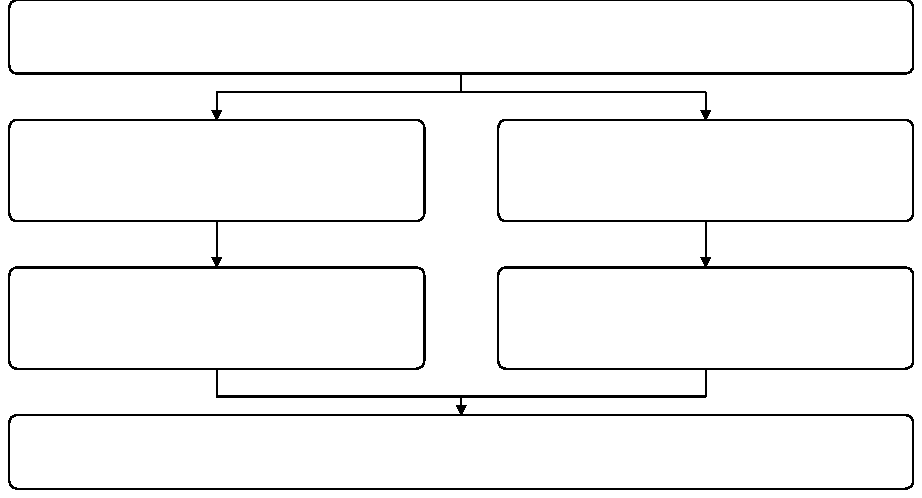
\includegraphics[width=\linewidth]{figures/rank_three_dimension_geometry.pdf}}
\put(50,50){\makebox(0,0){\parbox{94\unitlength}{\centering\fontsize{10}{12}\selectfont Ratio projection of $Y$ onto $\mathscr B$\\$\dim\mathscr B\in\{1,2\}$}}}
\put(23.5,35.5){\makebox(0,0){\parbox{41\unitlength}{\centering\fontsize{10}{12}\selectfont $\dim\mathscr B=2$\\Normal equations\\Algebraic differential obstructions}}}
\put(76.5,35.5){\makebox(0,0){\parbox{41\unitlength}{\centering\fontsize{10}{12}\selectfont $\dim\mathscr B=1$\\Curve tangency\\Direction and amplitude fibres}}}
\put(23.5,19.5){\makebox(0,0){\parbox{41\unitlength}{\centering\fontsize{10}{12}\selectfont Empty projective boundary\\$\dim Y_{\mathrm{gen}}=0$\\Proposition~\ref{r3:dominantfinite}}}}
\put(76.5,19.5){\makebox(0,0){\parbox{41\unitlength}{\centering\fontsize{10}{12}\selectfont Finite projective boundary\\$\dim Y_{\mathrm{gen}}\le1$\\Proposition~\ref{r3:curvefibre}}}}
\put(50,5){\makebox(0,0){\parbox{94\unitlength}{\centering\fontsize{10}{12}\selectfont $\dim Y=\dim\mathscr B+\dim Y_{\mathrm{gen}}\le2$\\$\operatorname{rank}d\mathsf X\le2$}}}
\end{picture}
\caption{The fibre dimension estimates for the ratio projection.}
\label{fig:rankthree-dimension}
\end{figure}

\subsection{Finite fibres over the ratio plane}\label{r3:ordinaryincoming}
Suppose that $\dim\mathscr B=2$. We work over the function field of
the ratio plane. A positive dimensional affine generic fibre would
have a point at infinity in its projective closure. The closure of
such a point gives a boundary component dominant over the ratio
plane. It is this type of component that must be excluded.

\subsubsection{The relative projective boundary}

Give the six off-diagonal coordinates weight one and the three
$\mathsf R_i$ weight two. Write
$\overline p=\tau\widehat p$ and $(\boldsymbol v)_j=\tau^2\mathsf R_j$ in the
weighted projective closure. The construction in
Appendix~\ref{r3:atlas} gives a proper modification equal to $Y$ on
the affine open set $\tau\ne0$. Choose an open neighbourhood
$\mathscr U$ of $(\eta,\zeta)=(1,-1)$ in the ratio plane as in that
construction. A boundary component dominating the plane is proper over
$\mathscr U$. Its image is closed and contains the generic point, hence
is all of $\mathscr U$. It therefore meets the fibre over $(1,-1)$.
Throughout this argument the entries of $\overline p$ are ordered as
$(12,13,21,23,31,32)$.

The weights reflect the degrees of the state equations: frame
coefficients have degree one, and their first derivative
coordinates have degree two. A single ordinary projective chart
would conflate these two growth scales. The modification separates
their relative orders by blowing up the loci where the weighted
derivative coordinates vanish. Properness brings a dominant
boundary component to the chosen ratio fibre; the blowup charts
give regular local equations at its points.

\begin{lemma}[Boundary coverage]\label{r3:boundarycoverage}
Fix positive, pairwise distinct principal values and suppose that
$\dim\mathscr B=2$. Consider a formal arc with generic point in $Y$
and special point on the boundary over $(\eta,\zeta)=(1,-1)$.
After a finite extension it lifts to the modification and the finite
covers of Appendix~\ref{r3:atlas}, with the following alternatives.
\begin{enumerate}[label=\textup{(\roman*)},leftmargin=*]
\item Put $n=\operatorname{ord}\tau>0$ and
$s_0=\min_j\operatorname{ord}(\boldsymbol v)_j$, with $s_0=\infty$
if $\boldsymbol v=0$ identically. The valuation regions are
\[
 s_0=0,\qquad 0<s_0<n/2,\qquad s_0=n/2,\qquad
 n/2<s_0<n,\qquad n\le s_0\le\infty.
\]
They lie, respectively, in the original weighted charts, the
supercritical charts, the common critical chart, the subcritical
charts and the ordinary charts.
\item In the intermediate regions $0<s_0<n$, the leading
representative $\overline{\boldsymbol R}$ has a nonempty coordinate
support. A support of size one leaves four possible
$\overline p$ coordinates and fifteen nonempty supports. A support of
size two leaves, up to cyclic relabeling, a single paired support,
two coordinate axes, a mixed support, or a nonzero paired group
together with at least one remaining coordinate. A support of size three has the three paired
groups $(12,32)$, $(13,23)$ and $(21,31)$.
\item On each support stratum, the simultaneous ranks of any finite
collection of regular coefficient matrices, together with the zero
and nonzero loci of finitely many regular coefficient factors,
define a finite locally closed refinement.
\end{enumerate}
Every closed point of a boundary component dominating the ratio plane over
$(1,-1)$ admits an arc of this form.
\end{lemma}

\begin{proof}
The two blowups are proper and have their centres in $\tau=0$.
Hence an arc from the affine locus lifts by the valuative criterion.
The auxiliary covers are finite and surjective, so the lift extends
to them after a finite extension of its complete discrete valuation
ring. A ramification index multiplies all orders by the same integer.

If $s_0=0$, a nonzero $(\boldsymbol v)_j$ selects an original weighted chart,
including points with $\overline p=0$. If $s_0>0$, some
$\overline p$ coordinate is nonzero. For finite $s_0$, choose an entry
$(\boldsymbol v)_j$ of least order. The chart equations are
\[
\begin{array}{c|c|c}
\text{chart}&\text{coordinates}&\text{orders}\\ \hline
W_{\mathrm O}&\boldsymbol v=\tau\boldsymbol R
 &\operatorname{ord}R_j\ge0\quad(s_0\ge n)\\
W_{\mathrm S}&\boldsymbol v=\kappa\delta\overline{\boldsymbol R},\quad
              \tau=\kappa^2\delta
 &(\operatorname{ord}\kappa,\operatorname{ord}\delta)
       =(n-s_0,2s_0-n)\\
W_{\mathrm T}&\boldsymbol v=\sigma\overline{\boldsymbol R},\quad
              \tau=\sigma^2\beta_{\mathrm T}
 &(\operatorname{ord}\sigma,\operatorname{ord}\beta_{\mathrm T})
       =(s_0,n-2s_0).
\end{array}
\]
Nonnegativity gives the regions in \textup{(i)}. At $s_0=n/2$,
$\delta$ and $\beta_{\mathrm T}$ are units and $\delta\beta_{\mathrm T}=1$ on the overlap.
If $s_0=\infty$, the ordinary chart has $\boldsymbol R=0$.

In an intermediate chart, choose $(\boldsymbol v)_j$ of least order and normalize
$\overline{\boldsymbol R}=\boldsymbol v/(\boldsymbol v)_j$. The finite auxiliary
coordinates $\boldsymbol e^{\mathrm{alg}}$ of Appendix~\ref{r3:atlas}
are regular on the lifted arc and satisfy
\[
 L(\overline p)\overline{\boldsymbol R}
       =\frac{\tau}{(\boldsymbol v)_j}\boldsymbol e^{\mathrm{alg}},\qquad
 \operatorname{ord}\frac{\tau}{(\boldsymbol v)_j}=n-s_0>0.
\]
Thus $L(\overline p)\overline{\boldsymbol R}=0$ at its special point.
Writing out the matrix $L$ of Appendix~\ref{appr3:sources} gives
\[
\begin{aligned}
\overline p_{12}\overline R_1
 &=\frac{\zeta-\eta}{\zeta(\eta+1)}
       \overline p_{32}\overline R_3,\\
\overline p_{13}\overline R_1
 &=\frac{\zeta-\eta}{\eta(\zeta-1)}
       \overline p_{23}\overline R_2,\\
\overline p_{21}\overline R_2
 &=\frac{\eta(\zeta-1)}{\zeta(\eta+1)}
       \overline p_{31}\overline R_3.
\end{aligned}
\]
Their coefficients are units in the ratio localization. With only
$\overline R_3\ne0$, they force
$\overline p_{31}=\overline p_{32}=0$, leaving the other four entries.
With $\overline R_2\overline R_3\ne0$ and $\overline R_1=0$, they
force $\overline p_{23}=\overline p_{32}=0$ and pair
$\overline p_{21}$ with $\overline p_{31}$. If this pair is the only
nonzero group, the support is paired. If it is zero, the remaining
coordinates give the two axes or their mixed support. If the pair
and at least one remaining coordinate survive, they give the last
alternative in \textup{(ii)}.
Cyclic permutations give three paired, six axis and three mixed
configurations. When all three $\overline R_i$ are nonzero, the
displayed relations give the three groups in \textup{(ii)}.
These incidence relations therefore allow
$3\cdot15+3\cdot7+7=73$ possible coordinate support patterns.

On a fixed support, a matrix has rank $r>0$ precisely where all its
$(r+1)$-minors vanish and at least one $r$-minor is nonzero; rank zero
means that every entry vanishes. These are finitely many locally
closed conditions. Each additional coefficient factor is then
partitioned into its zero and nonzero loci. Intersecting these finite
partitions proves \textup{(iii)}. On a paired chart put
$\overline p_{12}=1$, $\ell=\overline p_{32}$ and use $k=a\kappa_0$, $m=1+k$
as in Appendix~\ref{appr3:sources}. The two conditions
$m\ell^2=\pm k$ are disjoint, since
$2k\ne0$. Each is considered both on and off the material
resonance $k+q=0$. The local ideals are formed in the full local
ring, with the coefficient factors that vanish at the special point
retained as parameters.

Finally, the strict transform $\widetilde Y$ is the irreducible closure
of $Y$ in the modification. It is Noetherian, being of finite type
over $\mathbb C$. Its generic point lies in $Y$ and
specializes to every closed point of $\widetilde Y$.
A discrete valuation ring realizes this specialization
\cite[Lemma~28.5.10, Tag~054F]{StacksProject}; completing it gives
the required formal arc. A boundary component
dominating the ratio plane meets the selected fibre by properness.
\end{proof}

Let $J$
be the ideal of the closure of $Y$ in a
boundary chart. It is saturated:
\[
 J:\tau^\infty=J.
\]
The homogenized compatibility equations and their derivatives, after
division by powers invertible on the affine open set, generate an ideal
$I\subset J$. If $\tau^N\in I$, saturation gives $1\in J$, so the
chart contains no point of the closure of $Y$. The same conclusion
follows by excluding formal arcs whose generic points lie in
$\tau\ne0$: a point of the closure of an affine open set lies on such
an arc after a field extension. Normal equations are useful here
because they compare the first nonzero terms of an approaching arc.
A nilpotent normal coordinate vanishes on the arc, and a system of
weighted initial equations can force several normal coordinates to
vanish together.

Saturation also justifies division by an exceptional power when
the quotient is regular: if $\tau^dF\in J$, then $F\in J$.
This is the ideal-theoretic reason the divided equations remain
necessary equations for the solution closure. We retain $\tau$
in the local equations. A boundary point belonging to the closure
of the affine solution must admit an arc with $\tau\ne0$ at its
generic point. If the equations in $I$ force $\tau=0$ identically
on every such arc, that point is excluded from the closure.

\begin{lemma}[Exclusion by normal equations]\label{r3:normalexclusion}
Work in the completed local ring of a boundary chart. Let
$g_1,\ldots,g_r$ be normal coordinates vanishing at the point, and
suppose that $\tau^N\in I+(g_1,\ldots,g_r)$ for some integer $N>0$.
Assign positive integer weights to the $g_j$. Suppose that finitely
many equations in $I$, expanded in the $g_j$ with the parameters along
the family retained, have no terms below their respective weighted
degrees. After reducing the coefficients modulo the maximal ideal,
suppose that their initial forms have the origin as their only common
zero over the algebraic closure of the residue field.
Then no formal arc through the point, annihilating $I$, has a generic
point in $\tau\ne0$.
\end{lemma}
\begin{proof}
If some $g_j$ is nonzero along such an arc, minimize the quotient of
its order by its weight. After a finite ramified extension, the first
coefficients of the $g_j$ at this weighted order form a nonzero vector.
The first terms of the equations make every initial form vanish on
that vector, a contradiction. Hence all $g_j$ vanish on the arc, and
the inclusion $\tau^N\in I+(g_1,\ldots,g_r)$ gives $\tau=0$.
\end{proof}

There are two ways in which the local equations will be used.
First, suppose that all the equations vanish on a specified
family, and that their linear coefficient matrix in its normal
coordinates has full column rank. An invertible minor permits
implicit elimination of these coordinates in the completed local
ring. The zero normal coordinates already solve the full
equations, so uniqueness of the implicit solution makes the
eliminated coordinates zero. If $\tau$ is in this normal ideal,
the family has no approaching affine arc.

Second, a coefficient minor may vanish on a subfamily. On that
locus we eliminate only the coordinates belonging to an
invertible submatrix, using the full equations rather than their
linear parts. The equations in the remaining coordinates then
have well-defined weighted initial forms. If these forms have
only the zero solution and
$\tau^N\in I+(g_1,\ldots,g_r)$, the preceding lemma again
excludes an affine arc. The weighted initial forms include the
quadratic terms created by implicit elimination.
Lemmas~\ref{r3short:initial} and~\ref{r3short:schur} give the
corresponding local reductions.

Some boundary families require a normal ideal containing products
or squares of coordinates. If the compatibility relations belong to such an
ideal and their classes span its quotient by the maximal ideal,
Nakayama's lemma makes them generate the entire ideal. Membership
in the ideal is checked for the full polynomials, and spanning is
checked in this quotient. Thus the conclusion is an inclusion of
ideals in the completed local ring, even when the family has a
nonreduced normal structure. The powers and products are retained
until this inclusion has been obtained.
On the ordinary chart of the modification,
$\boldsymbol v=\tau\boldsymbol R$, with $\boldsymbol R$ a regular
coordinate vector on that chart.

\begin{lemma}[Reduction of the relative boundary]\label{r3:boundaryreduction}
Near the fibre $(\eta,\zeta)=(1,-1)$, every irreducible component
of the boundary of $Y$ dominating the ratio plane is contained,
up to a signed cyclic relabeling, in the family
\begin{equation}\label{r3:incomingfamily}
\begin{gathered}
 \mathcal F_{\rm in}:\quad
 \overline p=(1,0,0,0,0,\ell),\qquad
 \boldsymbol R=(\lambda_{\mathrm{in}}(v)\ell,u,v),\qquad
 \tau=0,\qquad \ell\ne0,\\
 \lambda_{\mathrm{in}}(v)=
 \frac{(\zeta-\eta)v-2\eta(\zeta+1)}{\zeta(\eta+1)}.
\end{gathered}
\end{equation}
Here $\overline p=\tau\widehat p$ and
$\boldsymbol R=\tau\mathsf R$ are ordinary homogeneous coordinates.
The homogeneous regularizations of the state derivations on the
ordinary projective closure preserve the surviving boundary component.
\end{lemma}
\begin{proof}
Let a boundary component dominate the ratio base. By properness
it meets the fibre $(1,-1)$. We examine the approaches
from the affine locus to this fibre, using the necessary ideal
$I\subset J$ and Lemma~\ref{r3:normalexclusion}.

For an approaching arc, use the orders $n,s_0$ and the support
alternatives of Lemma~\ref{r3:boundarycoverage}. On each support
we retain the coefficient factors
at a rank drop and their intersections with the special
principal value loci in the local coefficient ring.

The local equations on these supports have two exclusion mechanisms.
Where a normal coefficient matrix has full column rank, its selected
relations generate the required normal ideal and force a power of
$\tau$ into $I$. On its rank strata, one first eliminates the coordinates belonging
to an invertible submatrix using the full local equations. The remaining normal equations
have initial homogeneous forms with no nonzero common zero, or
generate an ideal containing the required exceptional coordinate.
Lemma~\ref{r3:normalexclusion} forces $\tau=0$ on such an arc.
At the four-point family, implicit elimination gives two normal
ideals describing the local families through those points. The
remaining equations generate their intersection. The eliminated
expression for $\tau$ belongs to both ideals, hence to their
intersection. Pulling this membership back gives $\tau$ in the
original local ideal, including at the intersection of the two
families. Appendix~\ref{r3:boundarysources} gives the generators.

The conic endpoint with $\overline p_{23}=0$ and one nonzero
leading derivative coordinate requires an exact relative ideal.
On its intermediate chart,
$\boldsymbol v=\kappa\delta\overline{\boldsymbol R}$ and
$\tau=\kappa^2\delta$. Six complete equations with an invertible
Jacobian define an implicit graph. The reference conic ideal on
this graph is generated by one coordinate and the square of
another. A first residual is divisible by $\overline p_{23}$,
and its regular quotient, together with a second residual,
has an invertible coefficient matrix in these two generators.
Thus $\overline p_{23}$ times the reference ideal belongs to the
necessary ideal. The coordinate $\kappa$ belongs to the reference
ideal, while $\delta$ is divisible by $\overline p_{23}$, giving
\[
 \kappa\delta\in I,\qquad \tau=\kappa^2\delta\in I.
\]
Appendix~\ref{appr3whole:identities} gives this local proof with
$\eta,\zeta$ retained as parameters. Since $I\subset J$ and
$J:\tau^\infty=J$, this endpoint is excluded from the relative
closure of the affine state image.

For each coefficient used in elimination, its nonvanishing set permits
division and its zero locus is treated with the original equations.
This gives a further partition of each support by coefficient rank.
On the paired supports, the coefficient rank can drop on the
two amplitude hypersurfaces
\[
 (1+a\kappa_0)\ell^2=a\kappa_0,
 \qquad (1+a\kappa_0)\ell^2=-a\kappa_0.
\]
Their difference is $2a\kappa_0\ne0$, so they are disjoint.
The material resonance in these strata is
\[
 a\kappa_0^2=(1+a\kappa_0)q
 \quad\Longleftrightarrow\quad a\kappa_0+q=0.
\]
It is kept as a parameter condition when either amplitude
hypersurface is considered. In the critical missing-row stratum,
the original equations would require
\[
 1+\frac{b(a-1)^2}{a(b-1)^2}=0,
\]
which is impossible because $a,b>0$. On the canonical paired
stratum, simultaneous vanishing of the elimination minors at
the material resonance would require
\[
 -\kappa_0(1+\kappa_0)=\frac34.
\]
But $-\kappa_0(1+\kappa_0)=\frac14-(\kappa_0+\frac12)^2\le\frac14$.
On the inactive paired stratum, elimination at the resonance leaves
one normal coordinate whose quadratic coefficient is
\[
 -\frac{16q}{\kappa_0}
       \left((\kappa_0+\tfrac12)^2+3\right)\ne0.
\]
The remaining equation is a unit times the square of that coordinate
in the completed local ring. That coordinate must therefore vanish on
every reduced formal arc annihilating $I$, and the implicit equations force the exceptional coordinate
to vanish. The other coefficient zero sets give either an ideal
containing $\tau$ or the initial forms of
Lemma~\ref{r3:normalexclusion}, as specified in
Appendix~\ref{r3:boundarysources}.

On the other intermediate supports we use differential invariance
to pass from the selected fibre to a neighbourhood in the base.
The state derivations extend after homogeneous regularization on
the weighted Rees model with integer weights $(n,2n-s_0)$. Put
$\gamma=2-s_0/n$. For each monomial of a regularized derivation, the
exponent of the exceptional parameter is affine in $\gamma$.
The endpoint degree bounds in Appendix~\ref{appr3:fielddegrees}
make this exponent nonnegative at $\gamma=1,2$, and therefore
throughout $1<\gamma<2$.
On the supports with two available horizontal fields, their base
minor is nonzero and the resulting boundary component dominates
the ratio base. On full derivative support with at least two surviving
amplitude pairs, the induced derivations fix the amplitude and direction
parameters and act independently on
$\eta,\zeta$. The ratios are algebraically independent over the
common constant field, so the compatibility equations can be compared
coefficientwise (Appendix~\ref{r3logic:boundaryconstants}).
On a transverse local chart, Lemma~\ref{r3logic:formalbasetransfer}
transfers the radical inclusion from the selected fibre to the full
local ring: the formal flows preserve $J$ and multiply $\tau$ by
a unit. The supports lacking these fields were treated by the
relative local identities above.

Coefficient comparison here takes place in a function field
where the direction parameters are common constants and the
ratios are algebraically independent over those constants.
Formal transfer uses two regular lifted fields with an
invertible base minor. Their formal flows preserve the saturated
ideal and send the boundary equation to a unit multiple of
itself, so they transport a radical inclusion forcing $\tau=0$
from the selected fibre to the relative local ring. At a point
where the base minor vanishes, the relative local identities
above supply the exclusion.

In the ordinary chart, the remaining local ideals give the
radical inclusion
\[
 (\overline p_{13},\overline p_{21},\overline p_{23},
   \overline p_{31},
   (\boldsymbol R)_1-\lambda_{\mathrm{in}}(v)\overline p_{32})
       \subset\sqrt{I+(\tau)}.
\]
Here the projective normalization is $\overline p_{12}=1$,
and $u=(\boldsymbol R)_2$, $v=(\boldsymbol R)_3$. The normal ideals giving this inclusion
are written in Appendix~\ref{r3:boundarysources}. Their squares
and cubes force the residual normal coordinates to vanish on
the reduced boundary; the quadratic change of coordinates on
the resonant stratum has the same radical. Hence a nonempty
open subset of the component satisfies
\eqref{r3:incomingfamily}.
Since this family is relatively closed, irreducibility puts the
generic point of the component in it. On the ordinary projective closure,
Lemma~\ref{r3logic:boundaryfields} applies to the invariant
prime $\mathfrak p$ and its saturated homogeneous closure. Its regularized
derivations preserve the minimal primes of the boundary ideal,
which gives the last assertion.
\end{proof}

The surviving family still has the three boundary coordinates
$\ell,u,v$. Reduction to this family therefore does not yet give
a fibre dimension bound. The next argument uses its induced
differential equations: it first makes a boundary coordinate
algebraic over the ratios and the common constants, and then
excludes the resulting algebraic differential equation.

\subsubsection{Differential equations on the ordinary boundary family}

The necessary homogenized equations vanish on
$\mathcal F_{\rm in}$. To exclude a dominant component in this family,
the normal coefficient matrices must be singular: an invertible
normal matrix would put $\tau$ in the compatibility ideal,
contradicting saturation. The induced derivations also preserve the
component. The singular normal matrices make certain boundary
coordinates algebraic, while differential invariance gives equations
incompatible with that algebraicity.

On $\mathcal F_{\rm in}$, set
\begin{equation}\label{r3:ordinary-boundary-coordinates}
 \Theta=(\zeta-\eta-1)v-2\eta\zeta,\qquad
 \beta=\frac{\eta(\zeta-1)}{\zeta(\eta+1)}.
\end{equation}
Away from $(v+2)\Theta=0$, two boundary derivations have independent
base components and can be normalized to induce
$\partial_\eta,\partial_\zeta$. Their equations and normal terms are
given in Appendix~\ref{appr3:ordinaryalgebraicity}.

The normalized fields send $(\eta,\zeta)$ to $(1,0)$ and
$(0,1)$, respectively. We use their common constant field to
compare coefficients. After fixing $\eta$, the second field
induces $d/d\zeta$ on the ratio field. The loci $v=-2$ and
$\Theta=0$, where the normalization fails, are treated separately
in Proposition~\ref{r3:ordinaryexclusion}.

\begin{lemma}[Algebraicity on the ordinary boundary family]
\label{r3:ordinaryalgebraicity}
Let $E$ be the function field of an invariant irreducible component of the boundary contained in $\mathcal F_{\rm in}$ and dominant
over the ratio plane. Suppose that the component is contained in
neither $v=-2$ nor $\Theta=0$. Let $C$ be the common constant field of
the two normalized horizontal derivations. Then $\eta,\zeta$ are
algebraically independent over $C$. Away from $v=2\eta$, the coordinate
$v$ is algebraic over $C(\eta,\zeta)$, including on $u=0$.
On $v=2\eta$, the coordinate $u/\beta$ is algebraic over that field.
\end{lemma}
\begin{proof}
The two derivations annihilate $\ell$ and, where it is defined, the
quantity
\[
 \frac{u^2}{\beta^2(v+2)(v-2\eta)}.
\]
A polynomial relation of least total degree between $\eta,\zeta$
over $C$ would have both partial derivatives zero. In characteristic
zero this is impossible.

Thus the two ratio coordinates remain independent even after
adjoining the first integrals to the constant field. This is the
field over which the coefficient comparison must be made. A
polynomial equation with coefficients depending on $\ell$ and the
displayed first integral is an equation over
$C(\eta,\zeta)$, because both of those quantities lie in $C$.
To prove algebraicity of $v$, it remains to show that at least one
of the necessary polynomial equations is nonzero in this field;
the vanishing of all its coefficients would supply no such
conclusion.

Consider the matrix of linear normal terms of the compatibility
relations along the family. A unit maximal minor would make the full
relations generate the normal ideal, which contains $\tau$.
Lemma~\ref{r3:normalexclusion} would exclude that point from the
closure of $Y$. The normal
minors consequently vanish on the component. Substitution of
the displayed constant quantity gives polynomial equations for $v$
over $C(\eta,\zeta)$. Their coefficient factorization in
Appendix~\ref{appr3:ordinaryalgebraicity} separates the two amplitude
hypersurfaces
\[
 (1+a\kappa_0)\ell^2=\pm a\kappa_0.
\]
Off these hypersurfaces, two coefficient vectors have a minor equal
to $63$. Their simultaneous vanishing forces
$\kappa_0\ell^2+q=0$ and the displayed first integral to equal $-q$.
On the positive amplitude hypersurface, a linear combination of two
coefficient conditions is a nonzero multiple of $a\kappa_0^2$.
On the negative hypersurface, the constant coefficient in $v$ is a
unit times $(a\kappa_0)^4$ times the first integral, which is nonzero
here. On the remaining locus where the first integral equals $-q$,
the coefficient of $v^4$ has two parameter coefficients with a
linear combination $-24a\kappa_0^2$. Its additional factor
$a\kappa_0+q$ can vanish only on the negative amplitude hypersurface
already treated. Hence the normal minors give a nonzero equation
for $v$.

On $u=0$, one retains the mixed normal generator $un_\perp$ and the
quadratic generator $n_\perp^2$, with $n_\perp$ as in
\eqref{appr3:ordinarynormals}. Two leading coefficients of the
resulting equations in $v$ contain, up to nonzero factors,
$5\kappa_0\ell^2+4q$ and $4\kappa_0\ell^2+5q$. They cannot both
vanish, since
\[
 5(4\kappa_0\ell^2+5q)-4(5\kappa_0\ell^2+4q)=9q\ne0.
\]
The factorization of the coupled normal columns in the same appendix
then gives a nonzero polynomial in $v$.

The mixed generator $un_\perp$ is kept even though the value of
$u$ is zero on the subfamily. Dividing it by $u$ would change the
local ideal and would remove precisely this case. The quadratic
generator $n_\perp^2$ records the remaining normal equation when
the linear column degenerates. The two coefficient factors above
show that the resulting polynomial conditions cannot both become
identically zero; they give algebraicity of $v$ on this subfamily
without inverting $u$.

On $v=2\eta$, the normal equations instead give a polynomial in
$u$. After unit factors are removed, its three-column normal factor
has highest $\zeta$ coefficient
\[
 -16(1+a\kappa_0)q(\eta+1)^5\ell^2\ne0.
\]
Thus this polynomial is nonzero, and $u/\beta$ is algebraic because
$\beta$ belongs to $C(\eta,\zeta)$ and is nonzero. At $u=0$ the
corresponding normal generators contain $\tau$, excluding the
component directly.
\end{proof}

We now hold $\eta$ fixed and regard $\zeta$ as the independent
variable. An algebraic function of $\zeta$ defines a finite covering
of the projective line. Residues of differentials and pole orders on
this covering give obstructions to the induced boundary equations.

\begin{lemma}[Algebraic differential obstructions]\label{r3logic:residue}
Let $K$ be a field of characteristic zero and let $E/K(\zeta)$ be
finite. Fix $\eta\in K$ with $\eta(\eta+1)\ne0$. If $v\in E$ satisfies
\[
 \frac{dv}{d\zeta}=
 \frac{(v-2\eta)(v+2)}{(\zeta-\eta-1)v-2\eta\zeta}
\]
with nonzero denominator, then $v=-2$ or $v=2\eta$.
The logarithmic derivative of a nonzero algebraic function in $E$
cannot be a nonzero constant in $K$.
\end{lemma}
\begin{proof}
Extend the constant field algebraically and pass to the smooth
projective curve of the resulting function field. If $v$ is nonconstant, its equation gives
\begin{equation}\label{r3:residue-identity}
 d\left(\frac{\zeta}{v+2}\right)
 =-\frac{(\eta+1)v}{(v-2\eta)(v+2)^2}\,dv.
\end{equation}
A nonconstant rational function on a smooth projective curve
maps onto the projective line, so there is a point above
$v=2\eta$. The differential on the right of
\eqref{r3:residue-identity}, considered first on the $v$-line, has
residue $-\eta/[2(\eta+1)]$ there. If $v-2\eta$ has order $e>0$
at a point of the covering curve, pullback multiplies this residue
by $e$. It remains nonzero. On the other hand, in a local
parameter the derivative of a Laurent series has no coefficient
of order $-1$. The exact differential on the left therefore has
residue zero at every point. This contradiction makes $v$
constant. Its differential equation then reduces to
$(v-2\eta)(v+2)=0$.

For the logarithmic assertion, a nonzero algebraic function has
the form $t^e$ times a unit at any point, so its logarithmic
differential has at most a simple pole there. At a point above
$\zeta=\infty$, write $\zeta$ as $t^{-r}$ times a unit with $r>0$.
Then $d\zeta$ has pole order $r+1\ge2$. Equality of a logarithmic
differential with a nonzero constant multiple of $d\zeta$ is
impossible.
\end{proof}

\begin{proposition}[Exclusion of the ordinary boundary family]
\label{r3:ordinaryexclusion}
No invariant irreducible component of the boundary contained
in $\mathcal F_{\rm in}$ dominates the ratio plane.
\end{proposition}
\begin{proof}
The hypersurface $\Theta=0$ is transverse to an induced derivation:
on it the derivative of $\Theta$ is
$4(\zeta-1)\eta(\eta+1)/(\zeta-\eta-1)$.
Thus it cannot contain an invariant dominant component.
Away from this hypersurface and $v=-2$, the normalized derivation
$D_\zeta$ fixes $\eta$ and satisfies
\begin{equation}\label{r3:ordinary-boundary-equations}
 D_\zeta v=\frac{(v-2\eta)(v+2)}{\Theta},\qquad
 D_\zeta\ell=0,\qquad
 D_\zeta(u/\beta)=\frac{v+1-\eta}{\Theta}(u/\beta).
\end{equation}
By Lemma~\ref{r3:ordinaryalgebraicity}, the field
$C(\eta)(\zeta,v)$ is finite over $C(\eta)(\zeta)$.
It is preserved by $D_\zeta$, whose extension is unique in
characteristic zero. Lemma~\ref{r3logic:residue} gives $v=2\eta$.
On the locus $v=2\eta$, the normal relations exclude $u=0$, while
\begin{equation}\label{r3:logarithmic-obstruction}
 D_\zeta\log(u/\beta)=-\frac1{2\eta}.
\end{equation}
The algebraicity of $u/\beta$ contradicts the second assertion of
Lemma~\ref{r3logic:residue}.

On $v=-2$, use the relative normal generators in
\eqref{appr3ord:Jnine}--\eqref{appr3ord:Jeleven}. The ideals
$J_9,J_{10},J_{11}$ correspond to the ordinary stratum and to the
two amplitude hypersurfaces above. Each has $\tau$ among its linear
generators. The compatibility polynomials belong to the relevant
ideal, and their coefficient classes span its quotient by the
maximal ideal times that ideal. Nakayama's lemma therefore gives
\[
 \tau\in J_j\subset I,\qquad j=9,10,11.
\]
On the negative amplitude hypersurface a quadratic change of normal
coordinates produces $J_{11}$ and leaves $\tau$ unchanged. The
coefficient matrices and this change are given in
Appendix~\ref{appr3ord:complete}. If $a\kappa_0+q=0$, the unit
coefficient matrix is obtained at the base point $(1,-2)$ in place
of $(1,-1)$. Thus $\tau\in I$ on a nonempty base open set, contrary
to saturation for a component dominant over the ratio plane.
\end{proof}

Dominance is used here only to pass to a nonempty open set of
the base. An irreducible component dominating the ratio plane
has its generic point over every such open set. Thus a unit
coefficient matrix near $(1,-2)$ excludes the same putative
component even if that matrix is singular at $(1,-1)$.
Here the coefficient matrix is computed for the relative normal
ideal on $v=-2$ at the replacement base point.

\begin{proposition}[Finite fibres over the ratio plane]
\label{r3:dominantfinite}
If the state image is dominant over the ratio plane, its generic
state fibre is finite.
\end{proposition}
\begin{proof}
An affine generic fibre of positive dimension would give a boundary
component dominant over the ratio plane. Properness forces it to
meet $(\eta,\zeta)=(1,-1)$. Lemma~\ref{r3:boundaryreduction} puts its
generic point in $\mathcal F_{\rm in}$, contradicting
Proposition~\ref{r3:ordinaryexclusion}. The generic boundary is empty.
Consequently the affine generic fibre is also proper. A proper affine
variety over a field is finite; see
Lemma~\ref{r3logic:propercriterion}.
\end{proof}

In particular, the estimate concerns the generic fibre over
$\mathbb C(\eta,\zeta)$. Special fibres over lower dimensional
subsets of the ratio plane may have larger algebraic zero sets;
they do not alter the transcendence degree of $\mathbb C(Y)$
over the ratio field. They will enter the proof only if the
entire ratio image is a curve, which is the next case.

\subsection{Fibres over an algebraic ratio curve}\label{r3:curves}

Suppose that $\dim\mathscr B=1$. If $\eta$ is constant, the cyclic
relabeling
\[
 (a',b')=(b/a,1/a),\qquad
 \eta'=-\zeta/\eta,\qquad \zeta'=-1/\eta
\]
makes $\eta'$ nonconstant. We may therefore work in
$\mathbb C(\mathscr B)$ with
\[
 \varsigma=\frac{d\zeta}{d\eta},\qquad
 L=\eta\varsigma-\zeta.
\]
The derivative with respect to $\eta$ extends uniquely from
$\mathbb C(\eta)$ to the function field of the curve, since the
extension is finite and separable. In particular, every derivative
of $\varsigma$ occurring below belongs to this field.

Tangency gives $E_i\zeta=\varsigma E_i\eta$. On the solution open
set where $d\eta\ne0$, differentiating this equation gives the
curve compatibility relations. After clearing denominators, they
belong to $\mathfrak p$ by analyticity and constrain the generic
fibre of $Y$.

The slope $\varsigma$ is a rational function on the ratio curve.
Pointwise elimination treats its value as a parameter. Along the
curve, the equations $\zeta'=\varsigma$ and the differentiated
compatibility relations further constrain the exceptional
direction families.

The smaller base permits a larger state fibre. An affine
irreducible component of dimension $d\ge1$ has boundary of
dimension $d-1$ in its projective closure. We therefore need only
show that its boundary is finite. Tangency to the ratio curve
adds the equations that will give this bound.

We make the parameter distinctions at the generic point of
$\mathscr B$. Since $\eta$ is nonconstant, every nonzero polynomial
in $\eta$ is a unit in $\mathbb C(\mathscr B)$. A polynomial in the
curve coordinates either vanishes identically or is a unit there.
Thus isolated exceptional ratio values do not form a further
generic branch; a coefficient zero set matters precisely when it
contains the ratio curve. The original localization is
\[
 \eta\zeta(\eta-\zeta)(\eta+1)(\zeta-1)\ne0.
\]
The additional characteristic conditions are
\begin{equation}\label{r3:characteristic-loci}
 \varsigma-1=0,\quad L+1=0,\quad L+\varsigma=0,\quad
 \varsigma=0,\quad L=0.
\end{equation}

Write
\[
 g_*=\eta\zeta(\eta-\zeta)(\zeta-1)(\eta+1)(1+\eta-\zeta)
       (\varsigma-1)(L+1)(L+\varsigma)\varsigma L.
\]
\begin{equation}\label{r3:quadratic-factor}
 \mathcal P_0=
 \eta\zeta(\eta^2-1)\varsigma^2
 -2(\eta^2-\zeta^2)\varsigma+\eta\zeta(1-\zeta^2).
\end{equation}

The factors of $g_*$ arise from the reconstruction and direction
equations, and $\mathcal P_0$ is the additional quadratic factor
of the direction determinant. At the generic point, first separate
$\zeta=\eta+1$, then the five conditions in
\eqref{r3:characteristic-loci}. On their complement, $g_*$ is a
unit, and $\mathcal P_0$ either vanishes or is a unit. This is the
partition in Table~\ref{tab:ratio-branches}.

Each row of the table is a condition in the function field of
one irreducible curve, rather than a condition at an isolated
point. A product vanishes in this field only if one of its factors
vanishes identically. The rows are taken in order, so intersections
are assigned to the first applicable row. After these rows have
been removed, the factors in $g_*\mathcal P_0$ are units and may
be used in rational reconstruction. The equations before those
divisions are used in the earlier rows.

\subsubsection{Characteristic ratio curves}

\begin{table}[htbp]
\centering
\small
\renewcommand{\arraystretch}{1.12}
\setlength{\tabcolsep}{3pt}
\caption{Branches at the generic point of the ratio curve
$\mathscr B$. The rows are considered in the displayed order,
each outside the preceding rows.}
\label{tab:ratio-branches}
\begin{tabular}{@{}>{\raggedright\arraybackslash}p{0.23\linewidth}>{\raggedright\arraybackslash}p{0.30\linewidth}>{\raggedright\arraybackslash}p{0.18\linewidth}>{\raggedright\arraybackslash}p{0.24\linewidth}@{}}
\toprule
Condition & Algebraic argument & Fibre conclusion & Proof location\\
\midrule
$\zeta=\eta+1$ &
Rational reconstruction and coprime quintic initial forms &
$\dim Y_{\mathrm{gen}}\le1$ &
Lemma~\ref{r3:balancedbound}; Appendix~\ref{r3:balancedline}\\
\addlinespace
$\varsigma=1$, $L=-1$, or $L=-\varsigma$ &
Affine pencils, Cramer numerators and compatibility &
$\dim Y_{\mathrm{gen}}\le1$ &
Appendix~\ref{appr3fib:pencils}\\
\addlinespace
$\varsigma=0$ or $L=0$ &
The first nonzero homogeneous terms of the original equations &
$\dim Y_{\mathrm{gen}}\le1$ &
Appendix~\ref{appr3fib:support}\\
\addlinespace
$g_*\ne0$, $\mathcal P_0=0$ &
Direction equations and tangency to the projected factors &
Finite projective boundary &
Appendices~\ref{appr3fib:support} and~\ref{appr3fib:Bwall}\\
\addlinespace
$g_*\mathcal P_0\ne0$ &
Direction and amplitude bounds; slope elimination &
Finite projective boundary &
Proposition~\ref{r3:directioneliminants}; Lemma~\ref{r3:contactelimination}\\
\bottomrule
\end{tabular}
\end{table}

The first three conditions in \eqref{r3:characteristic-loci}
integrate, respectively, to
\[
 \zeta=\eta+c,\qquad \zeta=1+c\eta,\qquad
 \zeta=c(\eta+1).
\]
Their common branch $\zeta=\eta+1$ is treated separately below.
The undivided zero pair equations treat a persistent vanishing
opposite pair. On the remaining chart, two compatibility
equations form an affine system for two pair coordinates over
three other pair coordinates. Its three coefficient rank strata
give the following dimension counts.

At rank two, the first two coordinates are reconstructed.
The remaining equations give two coprime polynomials in the
three base coordinates, so their common zero set has dimension
at most one. At rank one, consistency imposes a Cramer numerator
as well as the determinant. The determinant is irreducible and
does not divide that numerator, again giving base dimension at
most one. The third compatibility equation cuts the affine
kernel line in finitely many points and adds no fibre dimension.
At rank zero, and on the zero-column loci where this last
equation can degenerate, the compatible base is finite and the
residual equations bound the remaining fibre dimension by one.
Appendix~\ref{appr3fib:pencils} gives the determinants, Cramer
numerators and residual equations on these strata.

The last two conditions in
\eqref{r3:characteristic-loci} give $\zeta=c$ and $\zeta=c\eta$.
On these branches the highest homogeneous terms can cancel; the
next nonzero terms of the original equations give the required
bound, as shown in Appendix~\ref{appr3fib:support}.

\begin{lemma}[The ratio line $\zeta=\eta+1$]\label{r3:balancedbound}
On the persistent branch $\zeta=\eta+1$, the generic state fibre
has dimension at most one.
\end{lemma}
\begin{proof}
Tangency makes a fixed diagonal multiple of the normalized curl
matrix symmetric. The original relations exclude a persistent
zero opposite pair. On the remaining open set, three pair
coordinates reconstruct the complete state rationally. Two
necessary polynomials in those coordinates have coprime leading
forms of degree five for every admissible triple of principal
values and ratio. A common factor of the two polynomials would have a leading
homogeneous factor dividing both quintic forms, contrary to
their coprimality. A common zero set of dimension at least two
in these three coordinates would have a hypersurface component
and hence a common irreducible factor. Its dimension is therefore
at most one, and rational reconstruction transfers the bound to
the state fibre. Appendix~\ref{r3:balancedline} gives the
reconstruction, the leading forms and the zero pair argument.
\end{proof}

\subsubsection{Directions and amplitudes at infinity}

On $g_*\ne0$, the first tangencies give the rational coordinate change
\eqref{r3:directioncoordinates}. It expresses the three
$\mathsf R_i$ rationally in the six off-diagonal frame
coefficients. Consequently a dimension bound for these six
coordinates is also a bound for the complete generic state fibre.

Write the three opposite pairs as $(w_i,m_i)$ in these coordinates.
At infinity each nonzero pair has direction
$(w_i:m_i)\in\mathbb P^1$. Once direction representatives are
chosen, their amplitudes are defined up to one common multiplier.
The mixed equations first constrain these three projective
directions. For each permitted choice, the cubic and quartic
equations constrain the relative amplitudes. A finite set of
directions with finite projective amplitude fibres gives a finite
boundary. Directions with a zero coordinate are treated by retaining
the homogeneous equations on that coordinate support.

A direction specifies the ratio within a pair, whereas an
amplitude specifies its size relative to the other pairs. If all
three pairs are nonzero, the amplitudes form an open subset of
$\mathbb P^2$; with two pairs they form an open subset of
$\mathbb P^1$, and with one pair there is no relative amplitude
parameter. This separation avoids counting the common
homogeneous multiplier as a boundary coordinate. It also shows
why a direction bound alone is insufficient: even one fixed
direction can carry an amplitude curve.

The mixed equations are bilinear in pairs of directions. An
invertible coefficient block determines a projective map between its
two directions. With three invertible blocks, the direction fibre is
the fixed point set of their composition. A nonidentity projective
map of $\mathbb P^1$ has at most two fixed points. Its fixed point
equation vanishes identically precisely when the representing
matrix is scalar. With singular blocks, the determinant and trace
relations give the exceptional cases in
Appendix~\ref{appr3fib:support}.

Projection of these exceptional equations gives finitely many plane
polynomials. A factor depending only on $\eta$ is a unit. For a
nonvertical irreducible factor $f$, characteristic zero gives
separability in $\zeta$, so $f_\zeta$ is nonzero at the generic
point of $f=0$. Tangency therefore gives
$\varsigma=-f_\eta/f_\zeta$. Substituting this
slope into the original equations and clearing denominators gives
polynomials whose joint greatest common divisor with $f$ is $1$
in $\mathbb Q(\eta)[\zeta]$, as proved in
Appendix~\ref{appr3fib:support}. Their B\'ezout identity remains valid
in $\mathbb C(\mathscr B)$, where the nonzero denominators in $\eta$
are units. It contradicts simultaneous vanishing on a persistent
curve. The coefficient zero sets use the original bilinear equations
and their tangency relations before elimination. The mixed direction
fibre consequently has at most two points at the generic ratio point.

For proper supports and the seven full support patterns with
some $m_i=0$, the cubic and quartic relations also give finite
projective amplitude fibres. Passing to squared amplitudes is a
finite map, and the cubics are linear in those squares. For full
support, rank zero is excluded by the pure cubic coefficients and
tangency to their vanishing loci. At rank at least two, the
projective kernel is at most a point, whose inverse image contains
only finitely many amplitude points. At rank one, the projective
kernel is a line; a positive dimensional fibre would require a
common line component of the remaining quartic equations after
the substitution. For two nonzero pairs with amplitudes $x,y$, quartic combinations give
$\pm4x^2y^2$, so there is no amplitude curve on that support.
For three nonzero pairs, if the defining linear form of the kernel
line has a zero coefficient, the pure quartic terms
$xy(x+y)^2$ and $xy(x^2+y^2)$ force $xy=0$.
The six resulting configurations have coefficient ideals, augmented
by their first two curve derivatives, containing a unit on $g_*\ne0$
(Appendix~\ref{appr3fib:support}). They therefore cannot persist
on the ratio curve.

On $m_1m_2m_3\ne0$, put $t_i=w_i/m_i$. One direction requires
separate treatment:
\[
 t_1=\frac{\varsigma}{2\zeta},\qquad
 t_2=t_3=-\frac{L}{2\eta\zeta}.
\]
For this distinguished direction, the amplitude equations are
conics in the squared amplitudes. Since $g_*\ne0$,
$\eta\varsigma/\zeta\ne0,1$. The determinants in
Appendix~\ref{appr3fib:support} give a nondegenerate conic, and the
coefficient minor
\[
 -2(\eta\varsigma/\zeta-1)^2\ne0
\]
shows that the first two conics are not proportional.
If $\eta\varsigma/\zeta=1/2$, both degenerate, but the third conic
is nondegenerate and not proportional to either. At the other
permitted values at least one of the first two is nondegenerate.
A nondegenerate conic is irreducible, so its intersection with
a conic not proportional to it has no common component.
B\'ezout's theorem makes their projective intersection finite.
The finite squaring map transfers this conclusion to the original
pair amplitudes.

For full support directions other than the distinguished one,
use the affine coordinates $(U,V,w_*)$ of
\eqref{r3:momentcoordinates}. The distinguished direction is their
origin. The original equations are linear in the auxiliary vector
\[
 \xi=(UV,U,V,Q_*(w_*))^{\mathsf T},
\]
where $Q_*$ is the polynomial in
\eqref{r3:momentquadratics}. Its coordinates also satisfy
\[
 Q_*(w_*)\xi_2\xi_3-\xi_1\xi_4=0.
\]
The original relations imply that $\xi=0$ forces the
distinguished direction, so $\xi\ne0$ on the present branch.
The five linear equations give the matrix $M_*$; four of the
equations give the square matrix $M$, as defined in
Appendix~\ref{appr3:momentrepresentation}.

The linear equations determine possible auxiliary vectors.
The displayed quadratic relation then imposes the product
condition satisfied by the original coordinates. Eliminating
the direction parameter gives two necessary conditions:
$\mathcal P_1=0$ for the linear equations and
$\mathcal P_2=0$ for their compatibility with the quadratic
relation. These polynomials are defined in
Appendix~\ref{appr3:eliminants}.

\subsubsection{The quadratic condition and the remaining directions}

On $\mathcal P_0=0$, retain the original direction equations.
Appendix~\ref{appr3fib:Bwall} treats both determinant roots,
the leading coefficient, their collision locus and the reconstruction
minors. For a projected plane polynomial $f$, its curve tangency and
$\mathcal P_0=0$ imply
\[
 \eta\zeta(\eta^2-1)f_\eta^2
 -2(\zeta^2-\eta^2)f_\eta f_\zeta
 -\eta\zeta(\zeta^2-1)f_\zeta^2=0.
\]
After removal of the localization factors, the straight branches
and $(\eta+1)\zeta=\eta$, each norm or minor polynomial $f$ is
coprime to its displayed tangency polynomial in
$\mathbb Q(\eta)[\zeta]$ (Appendix~\ref{appr3fib:Bwall}).
The corresponding B\'ezout identities exclude a persistent curve
on $f=0$.

Substituting the tangent slope
$\varsigma=-f_\eta/f_\zeta$ in $\mathcal P_0$ and multiplying
by $f_\zeta^2$ gives the displayed polynomial. A nonvertical
irreducible curve contained in $f=0$ and satisfying
$\mathcal P_0=0$ would therefore make both polynomials vanish
in its function field, contrary to their B\'ezout identity.
On the remaining curve $(\eta+1)\zeta=\eta$, the original
full support direction ideal is the unit ideal over
$\mathbb Q(\eta)$.

For the distinguished direction,
$\varsigma'=\varsigma L/(\eta\zeta)$. Differentiation of
$\mathcal P_0=0$ therefore gives
\[
 \eta\zeta\bigl((\mathcal P_0)_\eta+
       \varsigma(\mathcal P_0)_\zeta\bigr)
       +\varsigma L(\mathcal P_0)_\varsigma=0.
\]
Its resultant with $\mathcal P_0$ has, outside the localization
factors and finite $\eta$-levels, only the factors
$\zeta+1$, $\zeta+\eta$ and $\eta^2+\zeta^2+1$.
The first two are the straight branches. The last is strictly
positive on the real ratio image, so it is nonzero in
$\mathbb C(\mathscr B)$. Together with the proper support and
amplitude bounds, these exclusions give a finite generic
projective boundary on $\mathcal P_0=0$.

On $g_*\mathcal P_0\ne0$, the determinant defines a finite degree
two divisor in the projective direction parameter. The linear
equations define a kernel line on this divisor. Taking the norm of
the quadratic relation along the divisor gives a polynomial
condition on $(\eta,\zeta,\varsigma)$, which must hold together
with the condition for existence of the kernel.

Vanishing of the affine leading coefficient places a root at
infinity. Vanishing of the discriminant makes two roots
coincide. The homogeneous determinant defines a divisor of
length two in either case, with multiplicity. Forming the norm
on this divisor includes both configurations.

\begin{proposition}[Conditions for the remaining directions]
\label{r3:directioneliminants}
Let $\mathscr B$ be the algebraic ratio curve of a
solution, with $\eta$ nonconstant, and suppose that
$g_*\mathcal P_0\ne0$ at its generic point. A compatible full
support direction with $m_1m_2m_3\ne0$, distinct from the
distinguished direction, satisfies $\mathcal P_1=\mathcal P_2=0$
in $\mathbb C(\mathscr B)$.
\end{proposition}
\begin{proof}
The nonzero auxiliary vector is annihilated by $M_*$, so its
five maximal minors have a common root in the projective
direction parameter. Write each of these quadratic minors in
the basis of the three homogeneous monomials of degree two.
Evaluation at that root gives a nonzero vector annihilated by
their coefficient matrix. The matrix consequently has rank at
most two, and all its three by three minors vanish.

The identities in Appendix~\ref{appr3:eliminants} give the
ideal of these coefficient minors as $(\mathcal P_1)$.
After $\mathcal P_1$ is factored out, the residual minors have
a linear combination equal to
$\varsigma^2(\varsigma-1)^2$ times a nonzero polynomial in
$\eta$. This is a unit at the generic point of the present
curve, so the vanishing minors imply $\mathcal P_1=0$.
The same unit identities make the two constant columns of the
transformed four-row matrix independent. Their six minor charts
cover the parameter base.

On each chart, Schur reduction leaves a two by two linear pencil.
The coefficient ideals for an identically zero determinant and
for rank at most two at a root both contain a nonzero polynomial
in $\eta$ times $\varsigma(\varsigma-1)\mathcal P_0$
(Appendix~\ref{appr3:determinantreduction}).
This element is a unit in the current function field.
The determinant is therefore a nonzero homogeneous quadratic,
and the matrix has rank three on its zero divisor. This divisor
is finite flat of degree two, and its kernel is an invertible line
on which the quadratic relation restricts.

On the determinant divisor the reduced pencil has rank one,
because its rank zero locus has been excluded by the coefficient
ideal. A nonzero entry gives a local generator of its kernel;
on overlaps these generators differ by a unit. Thus the kernel
is a line also at a multiple determinant root. The quadratic
relation restricts to a section on this line. The local kernel
generators and their unit transition factors define it on the
entire determinant divisor.

Construct the norm on the ambient regular parameter open set.
Locally trivialize the kernel line and write the restricted
quadratic relation as an element of the finite locally free
algebra of the determinant divisor. Its norm is the determinant
of multiplication by this element. Vanishing at a compatible
root makes multiplication noninvertible in that root's local
algebra, hence makes the norm zero. This statement also holds
when that local algebra is nonreduced at a double root.

The two adjugate columns give local kernel representatives.
Their resultants are nonzero, so the norm is a nonzero section
and defines a Cartier divisor. Every irreducible component of
this divisor occurs in both resultants. Their common factor
therefore bounds its support by
$\mathcal P_0\mathcal P_2=0$. On the present open set
$\mathcal P_0$ is a unit, leaving $\mathcal P_2=0$.
The homogeneous determinant includes roots at infinity.
Lemmas~\ref{r3schur:reduction} and~\ref{r3schur:norm} give the
Schur reduction and the polynomial identity for this norm.
\end{proof}

The conditions $\mathcal P_1=\mathcal P_2=0$ constrain a direction
at a fixed ratio point. For them to hold along the ratio curve,
their derivatives with respect to its nonconstant coordinate
$\eta$ must also vanish. Since $\zeta'=\varsigma$, differentiation gives
\begin{equation}\label{r3:curve-differentiation}
 (\mathcal P_j)_\eta+\varsigma(\mathcal P_j)_\zeta
       +(\mathcal P_j)_\varsigma\varsigma'=0,
       \qquad j=1,2.
\end{equation}
Cross multiplication eliminates $\varsigma'$ without division
and gives the polynomial $C_*$ of
Appendix~\ref{appr3:contactcalculation}. Put
$R=\operatorname{Res}_\varsigma(\mathcal P_1,\mathcal P_2)$ and
$T=\operatorname{Res}_\varsigma(\mathcal P_1,C_*)$.

Multiplying the first differentiated equation by
$(\mathcal P_2)_\varsigma$ and the second by
$(\mathcal P_1)_\varsigma$, then subtracting, cancels the
$\varsigma'$ terms. The identity also holds where either partial
derivative is zero. The actual curve thus supplies a common
root in $\varsigma$ for each resultant pair and satisfies
$R=T=0$. These differentiated conditions express persistence
along the curve.

Lemma~\ref{r3:contactelimination} gives a common factor $D_0$ and
\[
 \gcd(R/D_0,T/D_0)=1\quad\text{in }\mathbb Q(\eta)[\zeta].
\]
The B\'ezout identity for these quotients has coefficients in
$\mathbb Q(\eta)[\zeta]$. Clearing its coefficients gives an
identity with a nonzero polynomial in $\eta$ on the right.
That polynomial is a unit in $\mathbb C(\mathscr B)$, because
$\eta$ is nonconstant. If $D_0$ were nonzero in this field,
$R=T=0$ would make both quotients vanish, contradicting the
identity. Hence $D_0=0$. Since the curve function field has
no zero divisors, one of its seven irreducible factors vanishes
identically:

\begin{equation}\label{r3:exceptional-ratio-loci}
 \zeta=0,\quad\zeta=-1,\quad\zeta=-\eta,\quad
 \zeta=\eta,\quad\zeta=1,\quad\zeta=\eta+1,\quad
 (\eta+1)\zeta=\eta.
\end{equation}
The factors $\zeta$, $\zeta-\eta$, $\zeta-1$ and
$\zeta-\eta-1$ are units on $g_*\mathcal P_0\ne0$.
On $\zeta=-1$, differentiation gives $\varsigma=0$;
on $\zeta=-\eta$, it gives $L=0$.
On $(\eta+1)\zeta=\eta$,
$\varsigma=(\eta+1)^{-2}$ and direct substitution gives
$\mathcal P_0=0$. These three cases are the earlier rows of
Table~\ref{tab:ratio-branches}.

Each alternative therefore contradicts a factor being a unit
in $g_*\mathcal P_0$. No full support direction distinct from
the distinguished one can persist on the current ratio curve.

\begin{proposition}[Fibres over an algebraic ratio curve]
\label{r3:curvefibre}
If the ratio image is an algebraic curve, the generic state fibre
has dimension at most one.
\end{proposition}
\begin{proof}
After cyclic relabeling take $\eta$ nonconstant. The characteristic
branches, $\zeta=\eta+1$, and $\mathcal P_0=0$ have the asserted bound.
Outside them, the proper supports, the directions with some
$m_i=0$, and the distinguished direction have finite projective
amplitude fibres over a finite direction set. Every other
direction would satisfy $\mathcal P_1=\mathcal P_2=0$ and would
therefore force one of the excluded conditions
\eqref{r3:exceptional-ratio-loci}. The generic projective boundary
is finite. Its affine fibre has dimension at most one, and the
rational state reconstruction transfers this bound to all nine
fibre coordinates.
\end{proof}

\subsection{Proof of the rank bound}\label{r3:completion}
\begin{proof}[Proof of Theorem~\ref{r3:theorem}]
On a connected localized chart, $\dim\mathscr B=0$ is excluded by
Lemma~\ref{fnd:constantratio}. If $\dim\mathscr B=2$,
Proposition~\ref{r3:dominantfinite} gives $\dim Y_{\mathrm{gen}}=0$.
If $\dim\mathscr B=1$, Proposition~\ref{r3:curvefibre} gives
$\dim Y_{\mathrm{gen}}\le1$.
Lemma~\ref{r3short:rank} yields $\operatorname{rank}d\mathsf X\le2$
in both cases.

By Lemma~\ref{fnd:muwall}, the localized locus is dense on the
branch $h_1h_2h_3\ne0$. Every minor of order three of the smooth
state map \eqref{fnd:X} vanishes there. Continuity gives its
vanishing at every remaining point of that branch.
\end{proof}

\section{Classical branches and proof of the main theorem}\label{sec:completion}

The rank exclusions establish the integrability hypothesis in Kafadar's
classification. We combine this result with the classical classification
on regular invariant charts, continue the resulting germs analytically,
and prove the converse by constructing the pressure. The families are
those in \eqref{intro:family0}--\eqref{intro:family5}.

\subsection{Integrability of a principal plane field}

\begin{proof}[Proof of Theorem~\ref{completion:zerocontact}]
Suppose first that $h_1h_2h_3$ were nonzero at a point. After shrinking,
it is nonzero on an open ball $U$. Lemma~\ref{fnd:muwall} says that
each zero set of a normalization factor has empty interior in $U$. These
sets are closed, so the complement of their finite union contains a
nonempty open chart satisfying \eqref{fnd:protected}. On a connected such chart, the retained
state map $\mathsf X$ has constant rank by Theorem~\ref{fnd:rankconstant}.
Since its domain is three dimensional, its rank is one of $0,1,2,3$.

Ranks zero and one contradict Theorem~\ref{fnd:lowrankexclusion}.
Rank three contradicts Theorem~\ref{r3:theorem}. At rank two,
Proposition~\ref{sim:generator} gives one nonzero common similarity
generator with equal source and target scales. The normal forms in
Proposition~\ref{sim:types} leave exactly the six pairings with zero dilation factor
or a pair with a common nonzero dilation factor. The former are excluded by
Theorem~\ref{iso:theorem}, and the latter by
Theorem~\ref{dil:whole}. Thus every possible rank is excluded, proving
\begin{equation}\label{completion:contactproduct}
 h_1h_2h_3\equiv0.
\end{equation}

By Lemma~\ref{fnd:analyticity}, $B$ is analytic on each inverse-function
chart. Its distinct constant eigenvalues are $\lambda_i^{-1}$, and its labelled
spectral projectors are the analytic tensors
\[
 P_i=\prod_{j\ne i}\frac{B-\lambda_j^{-1}I}{\lambda_i^{-1}-\lambda_j^{-1}}.
\]
Projecting and normalizing fixed vectors gives analytic unit
eigenvectors on a small ball; their signs may be chosen to orient the
frame. Each $h_i=e_i\cdot\operatorname{curl}e_i$ is analytic and is
unchanged when $e_i$ changes sign. A finite product of analytic
functions on a connected domain can vanish identically only if one
factor vanishes identically. Applied to
\eqref{completion:contactproduct}, this gives a fixed label with
$h_i\equiv0$. Finally, the nowhere-zero one-form $\alpha_i=e_i^\flat$
satisfies $\alpha_i\wedge d\alpha_i=h_i\,\mathrm{vol}_g$, so Frobenius
gives the asserted local surfaces.
\end{proof}

\subsection{Constant principal values}
\label{completion:classical-exits}

Throughout this subsection the eigenvalues of $c=B^{-1}$ are constant.
Thus $c$ is a positive definite flat metric with $\det c=1$, and
$\operatorname{div}c$ and $\operatorname{div}c^{-1}$ are local gradients.
By Lemma~\ref{fnd:analyticity}, $c$ is analytic.

\begin{proposition}[Kafadar's classification]
\label{completion:kafadar}
Under these hypotheses on constant principal values the following statements hold.
\begin{enumerate}
\item If $c$ has a fixed Euclidean eigenvector on a neighbourhood, the
deformation is locally in $\mathcal F_0$ or $\mathcal F_5$.
\item If at least two eigenvalues coincide, $c$ has a fixed Euclidean
eigenvector locally. Consequently this case is also contained in
$\mathcal F_0\cup\mathcal F_5$.
\item If the eigenvalues are distinct and one principal direction is
normal to a local foliation by surfaces, the deformation is locally in
$\mathcal F_0$ or $\mathcal F_5$.
\end{enumerate}
\end{proposition}
\begin{proof}
These are the applications of Theorems 1, 2, and 3 of
\cite[p.~20]{Kafadar1972}, respectively. Theorem 1 assumes that the
Cartesian components of $c$ are represented by their local Taylor
series. Lemma~\ref{fnd:analyticity} supplies this hypothesis. By
\cite[\S5, pp.~25--27, equation (5.1)]{Kafadar1972}, besides constant
Cartesian tensors, the deformation has the form
\[
 r=AR,\qquad \theta=C\Theta+D\log R,\qquad z=EZ,
 \qquad A^2CE=1.
\]
After translations and fixed Euclidean coordinate changes, this is
$\mathcal F_5$ with $(\alpha,k,\beta,\gamma)=(A,C,D,E)$.
A constant Cartesian metric $c$ has an affine local Euclidean
realization, giving $\mathcal F_0$. Two local realizations of the same
flat metric differ by a fixed Euclidean motion.

Theorem 2, proved in \cite[\S3, pp.~20--23]{Kafadar1972}, gives the
fixed eigenvector in the repeated-value case, after which Theorem 1
applies. If all three values coincide, positivity and
$\det c=1$ give $c=I$, whose realizations are rigid motions.

For the third assertion, use Theorem 3 and its proof in
\cite[\S4, pp.~23--25]{Kafadar1972}, with the Taylor hypothesis in its
final fixed-direction step supplied as above. Its geometric assumption
is exactly the existence of a principal direction normal to coordinate
surfaces. In the notation of the present paper this means
$\alpha_i\wedge d\alpha_i=0$, or $h_i=0$, on a neighbourhood.
Frobenius' theorem gives the local foliation.
\end{proof}

\begin{corollary}[The constant-invariant classification]
\label{completion:constantclassification}
If both invariants are constant on a neighbourhood, the universal
deformation is locally in $\mathcal F_0$ or $\mathcal F_5$.
\end{corollary}
\begin{proof}
The characteristic polynomial fixes the eigenvalues of $c$.
For repeated values apply the second part of
Proposition~\ref{completion:kafadar}. For distinct values,
Theorem~\ref{completion:zerocontact} supplies a fixed principal label
with $h_i$ identically
zero on a neighbourhood. Apply Proposition~\ref{completion:kafadar}(3).\qedhere
\end{proof}

\subsection{Reduction of the invariant map}
\label{completion:variable-equations}

For constant invariants, two choices of energy supplied the equilibrium
equations used above. When the invariants vary, derivatives of the
arbitrary energy give additional restrictions. They reduce the
invariant map to one local parameter and place its level surfaces in
the setting of the classical regular patch classifications.

Work on a spatial inverse-function
chart and identify vectors and one-forms using the Euclidean metric.
Put
\[
 u=dI_1,\quad v=dI_2,\qquad
 \beta=(\operatorname{div}B)^\flat,\quad
 \delta=(\operatorname{div}c)^\flat.
\]
For a symmetric tensor $A$ and a one-form $\omega$, write
$A\omega=(A\omega^\sharp)^\flat$. Expanding the divergence in the
original stress equation gives
\begin{equation}\label{completion:pressureform}
 \frac12\,dp_W=
 W_1\beta-W_2\delta+W_{11}Bu
                  +W_{12}(Bv-cu)-W_{22}cv.
\end{equation}
Universality requires the right-hand side to be closed for every $W$.
Conversely, on a sufficiently small simply connected chart, this
closedness supplies the pressure for each $W$ by the Poincar\'e lemma.
This is the coordinate-free form of the pressure calculation in
\cite[pp.~468--469, equations (2.1)--(2.2)]{Ericksen1954}.

\begin{lemma}[Rank of the invariant map]
\label{completion:invariant-rank}
Every universal deformation satisfies
\begin{equation}\label{completion:rankone}
 dI_1\wedge dI_2=0
\end{equation}
at every point. On a chart where one invariant has nonzero differential,
that invariant may be used as a local parameter $U$, and
\[
 I_1=i_1(U),\qquad I_2=i_2(U),\qquad
 B\,dU=\lambda(U)dU,\quad c\,dU=\lambda(U)^{-1}dU.
\]
Here $\lambda>0$, and at least one of $i_1',i_2'$ is nonzero.
\end{lemma}
\begin{proof}
At a specified point the third-order jet of the function
$W(I_1,I_2)$ can be prescribed arbitrarily, for example by choosing a
cubic polynomial. In the exterior derivative of
\eqref{completion:pressureform}, the coefficients of
$W_{111},W_{222},W_{112},W_{122}$ give, respectively,
\begin{equation}\label{completion:highest-pure}
 u\wedge Bu=0,\qquad v\wedge cv=0.
\end{equation}
\begin{equation}\label{completion:highest-mixed}
 \begin{aligned}
 v\wedge Bu+u\wedge Bv-u\wedge cu&=0,\\
 v\wedge Bv-v\wedge cu-u\wedge cv&=0.
 \end{aligned}
\end{equation}
Suppose $u\wedge v\ne0$ at a point. The same condition holds on a
smaller neighbourhood. The pure identities give
$Bu=\alpha u$ and $cv=\gamma v$, where $\alpha,\gamma$ are smooth
positive functions. The first mixed identity then reduces to
\[
 (\gamma^{-1}-\alpha)u\wedge v=0.
\]
Thus $u$ and $v$ belong to a common two dimensional eigenspace of $B$
with eigenvalue $\alpha$. Symmetry and $\det B=1$ imply that its three
eigenvalues are $\alpha,\alpha,\alpha^{-2}$ throughout this
neighbourhood. Consequently
\[
 I_1=2\alpha+\alpha^{-2},\qquad
 I_2=\alpha^2+2\alpha^{-1},
\]
which makes $u\wedge v=0$, a contradiction. This proves \eqref{completion:rankone}.

On a chart with $dI_1\ne0$, take $U=I_1$; the constant-rank theorem
gives $I_2=i_2(U)$. If instead $dI_2\ne0$, use $U=I_2$. The appropriate
identity in \eqref{completion:highest-pure} gives the asserted
principal direction, even if the other invariant is constant.
On each connected level patch of $U$, the
characteristic polynomial of $B$ has constant coefficients, while the
continuous function $\lambda$ takes values in its finite set of
positive roots. Thus $\lambda$ is constant on that level patch.
Evaluating it on a local transverse section shows that the resulting
function of $U$ is smooth, and analytic under
Lemma~\ref{fnd:analyticity}.
\end{proof}

\begin{lemma}[Pressure on a regular invariant chart]
\label{completion:regular-pressure}
On a chart as in Lemma~\ref{completion:invariant-rank}, universality
implies
\begin{equation}\label{completion:divergences}
 \beta=b(U)dU,\qquad \delta=d(U)dU
\end{equation}
for scalar functions $b,d$. Conversely, the principal-direction
relations of that lemma together with
\eqref{completion:divergences} make
\eqref{completion:pressureform} locally exact for every strain energy $W$.
\end{lemma}
\begin{proof}
The last three terms in \eqref{completion:pressureform} are
$k_W(U)dU$, where
\[
 k_W=\lambda i_1'W_{11}
       +(\lambda i_2'-\lambda^{-1}i_1')W_{12}
       -\lambda^{-1}i_2'W_{22}.
\]
They are already closed. The coefficients of the remaining first and
second derivatives of the strain energy in its exterior derivative are
\begin{align*}
 d\beta=d\delta&=0,\\
 i_1' dU\wedge\beta&=0,\\
 i_2' dU\wedge\beta-i_1' dU\wedge\delta&=0,\\
 i_2' dU\wedge\delta&=0.
\end{align*}
If $i_1'\ne0$, the second identity gives
$dU\wedge\beta=0$, and the middle mixed identity gives
$dU\wedge\delta=0$. If $i_2'\ne0$, use the last and mixed identities
in the reverse order. Hence both forms are multiples of $dU$. Their closedness makes
their coefficients constant on connected level patches of $U$,
proving \eqref{completion:divergences}. Substitution in
\eqref{completion:pressureform} proves the converse: its right-hand
side is a scalar function of $U$ times $dU$.
\end{proof}

The preceding lemmas place each regular invariant chart in the setting
of the classical classification.

\subsection{Variable invariants on regular patches}
\label{completion:regular-classification}

\begin{proposition}[Classical classification on a regular patch]
\label{completion:regularclassification}
Let $V$ be a regular invariant chart, and restrict to a subchart on
which the multiplicities of the eigenvalues of $c$ are constant.
Then the deformation is locally one of
$\mathcal F_1,\mathcal F_2,\mathcal F_3,\mathcal F_4$.
Moreover the eigenvalue corresponding to $dU$ is simple on this
subchart. Every nonempty open set on which the invariant map has rank
one contains a nonempty subchart to which this statement applies.
\end{proposition}
\begin{proof}[Proof from the classical classification]
Denote the eigenvalue of $c$ along $dU$ by $c_1$ and the remaining
two by $c_2,c_3$. These labels are local, with $c_1$ determined by
the gradient. There are three cases.

If the three values are distinct, Ericksen's classification
\cite[\S4, pp.~476--485]{Ericksen1954} applies. The level sets of the
invariant parameter are parallel planes or concentric circular
cylinders; the spherical possibility is excluded in this case. The
resulting models are the block, sector, and cylindrical families
$\mathcal F_1,\mathcal F_2,\mathcal F_3$.

If $c_1\ne c_2=c_3$, the gradient eigenvalue is simple and
\cite[\S5, pp.~485--486]{Ericksen1954} completes the classification.
The planar and cylindrical possibilities give already listed
degenerations, and the spherical case gives $\mathcal F_4$, including
eversion with its compensating angular orientation.

If $c_1$ is repeated, Ericksen's \S6, pp.~486--489, covers only an
additional integrability assumption on the remaining principal
direction. The unrestricted case uses
\cite[Theorem 1.1, p.~138, proof pp.~154--158]{MarrisShiau1970}, with
the corrections in \cite[p.~406]{MarrisShiauCorr1970}. For nonconstant
invariants their result reduces the geometry to concentric circular
cylinders; the curves tangent to the distinguished simple principal
direction are circular helices. Martin and Carlson then test
the two cylindrical models under the condition that the eigenvalue
along the invariant gradient is repeated
and show that only constant-invariant degenerations remain
\cite[\S3, pp.~107--108]{MartinCarlson1976}. This case therefore
cannot occur on $V$. Their footnote on p.~106 records the needed
scope of Ericksen's cylindrical calculation: although it occurs in
the section headed by distinct eigenvalues, the cylindrical
classification itself requires universality and cylindrical level
surfaces, so it applies to the preceding reduction.

These are the classes $B_1,B_2,B_3$ of
\cite[p.~106]{MartinCarlson1976}. See also
\cite[Theorem 1.2, pp.~138 and 159]{MarrisShiau1970}.

Finally, a nonempty regular invariant open set has a smaller open set
of constant eigenvalue multiplicity: either the discriminant of its characteristic polynomial
is nonzero somewhere, or it vanishes throughout and one restricts
to a repeated-value patch. A triple eigenvalue would give $B=I$.
At such a point both invariants attain their lower bound $3$, so
both differentials vanish; hence no triple-value point lies in the
regular invariant set. In the repeated-value alternative the two
distinct eigenvalues have a positive gap locally, which fixes whether
the gradient belongs to the simple or repeated eigenspace. The three
cases above apply on this smaller patch.
\end{proof}

The classical result supplies a deformation on a regular invariant
patch, after restricting to constant eigenvalue multiplicity.
Ericksen removes the common critical set $\{dI_1=dI_2=0\}$ at the
start of the variable invariant argument \cite[p.~469]{Ericksen1954}.
To include that set and points where principal values coincide, consider the analytic
invariants pulled back to a connected reference neighbourhood.
Either both are constant, giving the classification already proved,
or their common critical set has empty interior. In the latter case
the proposition supplies a classical germ on a nonempty open subset.
The remaining step is to carry this fixed germ to the chosen point.

\subsection{Continuation of a classical germ}\label{completion:continuationsection}

The cylindrical and spherical charts used in the classical formulas
may omit an axis or a centre at which the Cartesian deformation is
regular.
For example, the removable-axis part of $\mathcal F_3$ is
\begin{equation}\label{intro:twisted-axis}
 \begin{aligned}
 \chi_\perp(X,Y,Z)&=\sqrt A\,\operatorname{Rot}(\delta Z+\theta_0)
                  \operatorname{diag}(1,k)(X,Y),\\
 \chi_3(X,Y,Z)&=Z/(Ak)+z_0,\\
 &A>0,\quad k\in\{1,-1\}.
 \end{aligned}
\end{equation}
Here $\delta$ is arbitrary. For $\mathcal F_5$, a regular interior axis
requires $\beta=0$ and $k=\pm1$, giving an affine map.

A classical germ fixes both its parameters and its source and target
Euclidean coordinates. On the regular domain of its formula, the
analytic identity theorem propagates equality with the
deformation. At a boundary of that domain, boundedness of the
deformation gradient either excludes the boundary or forces a removable
coordinate singularity. The following proposition describes these continuations.

\begin{proposition}\label{completion:continuation}
Let $\Omega$ be connected and let $\chi:\Omega\to\mathbb R^3$ be a real
analytic local diffeomorphism with $\det D\chi=1$. Suppose that on a
nonempty open subset it equals one of
\eqref{intro:family0}--\eqref{intro:family5}, in fixed source and target
Euclidean coordinates and with fixed parameters. Then every point of
$\Omega$ has a neighbourhood on which $\chi$ is a continuation of that
same model. The only removable coordinate boundaries are
\eqref{intro:twisted-axis} for $\mathcal F_3$, a rigid motion for
$\mathcal F_4$, and an affine map for $\mathcal F_5$.
\end{proposition}

\begin{proof}
Shrink the initial open subset to a connected patch. Keep the
parameters and the two Euclidean coordinate changes selected
on the initial patch. Denote by $\mathcal D$ the full regular source
domain of its displayed formula: for $\mathcal F_1$ it is
$\{2\alpha X+d>0\}$; for $\mathcal F_2$ and $\mathcal F_5$ it is
$\{R>0\}$; for $\mathcal F_3$ it is
$\{R>0,\ AR^2+B_0>0\}$; and for $\mathcal F_4$ it is
$\{R>0,\ \varepsilon R^3+B_0>0\}$. For $\mathcal F_0$ take
$\mathcal D=\mathbb R^3$. Here $R$ is distance from the fixed axis or
centre. Positive roots are used throughout.

Let $V$ be the connected component of $\Omega\cap\mathcal D$ containing
the initial patch. In the cylindrical models, use the angular covering
of $\mathcal D$, with the lift of $\Theta$ fixed on that patch. The
formula defines a single analytic Cartesian map $G_{\mathrm{mod}}$ on this covering.
If $\pi:\widetilde V\to V$ is the connected covering component containing
the lifted patch, the analytic identity theorem gives
\begin{equation}\label{completion:coveridentity}
                 G_{\mathrm{mod}}=\chi\circ\pi\quad\hbox{on }\widetilde V.
\end{equation}
The projection is onto $V$, by path lifting. Thus the same model gives
the germ of $\chi$ at every point of $V$. The models without a source
angle use the identical argument without a covering.

By \eqref{completion:coveridentity}, continuation around a loop in $V$
returns the same germ. For a loop of winding number
$n$, single-valuedness requires $\beta n=0$ in $\mathcal F_2$,
$\kappa n=0$ and $kn\in\mathbb Z$ in $\mathcal F_3$, and
$kn\in\mathbb Z$ in $\mathcal F_5$.

Suppose that $q\in\Omega\cap\partial V$. Then
$q\notin\mathcal D$: otherwise a small ball about $q$ contained in
$\Omega\cap\mathcal D$ and meeting $V$ would lie in the same component.
Consequently $q$ is a finite axis, centre, or root boundary of the
model. Choose a closed ball about $q$ contained in $\Omega$; $D\chi$ is
bounded there. Since equality on $V$ includes equality of derivatives,
we examine the coordinate boundaries.

\emph{The block and straightening models.}
For $\mathcal F_1$ the only boundary is $r=0$, where
\[
                  |\partial_X\chi|=|\alpha|/r\longrightarrow\infty.
\]
For $\mathcal F_2$ the boundary is $R=0$, and its derivative along the
unit angular direction satisfies
\[
        |D\chi(e_\Theta)|=\frac{\sqrt{\beta^2+\gamma^2}}{R}
                         \geq\frac{|\beta|}{R}\longrightarrow\infty.
\]
Both contradict boundedness, since $\alpha\beta\ne0$.

\emph{The cylindrical model.}
In $\mathcal F_3$, $A(k\gamma-\delta\kappa)=1$ in particular implies $A\ne0$.
If $r\to0$ and $R\to R_*>0$, then
\[
                    |\partial_R\chi|=|A|R/r\longrightarrow\infty.
\]
If $R\to0$ and $r\to r_*>0$, then
\begin{equation}\label{completion:cylangular}
          |D\chi(e_\Theta)|=\frac{\sqrt{k^2r^2+\kappa^2}}{R}
                           \longrightarrow\infty,
\end{equation}
because $k$ and $\kappa$ cannot both vanish. The only remaining possibility is
$R\to0$ and $r\to0$. It forces $B_0=0$, $A>0$, and
$r=\sqrt A\,R$. Equation \eqref{completion:cylangular} first gives $\kappa=0$.

The punctured ball obtained by removing the source axis from a sufficiently
small ball about $q$ is connected and lies in $\Omega\cap\mathcal D$.
It meets $V$ and hence lies entirely in $V$. On any angular wedge in
this punctured ball, \eqref{completion:coveridentity} supplies one fixed
angle branch. At the axial level $Z=Z_*$ of $q$, continuity gives
$\chi_\perp(q)=0$, and differentiability gives a real linear map
$L:\mathbb R^2\to\mathbb R^2$ such that
\begin{equation}\label{completion:axislinear}
 L(\cos\Theta,\sin\Theta)
  =\sqrt A\bigl(\cos(k\Theta+\delta Z_*+\theta_0),
                 \sin(k\Theta+\delta Z_*+\theta_0)\bigr)
\end{equation}
on an open interval of angles. Its norm is constant on that interval.
The quadratic identity
$v^{\top}(L^{\top}L-AI)v=0$ on an open circular arc implies $L^{\top}L=AI$.
Hence $L/\sqrt A$ is orthogonal; its angular rate on that arc is $+1$
or $-1$. Differentiating \eqref{completion:axislinear} therefore yields
$k=\pm1$.

The volume condition now gives $\gamma=1/(Ak)$, and the original model has
the Cartesian expression
\begin{equation}\label{completion:cylremoval}
 \begin{aligned}
 \chi_\perp(X,Y,Z)
   &=\sqrt A\,\operatorname{Rot}(\delta Z+\theta_0)
                    \operatorname{diag}(1,k)(X,Y),\\
 \chi_3(X,Y,Z)&=Z/(Ak)+z_0.
 \end{aligned}
\end{equation}
This is analytic on all of $\mathbb R^3$, has determinant one, and
agrees with the initial model. The parameter $\delta$ remains arbitrary.

\emph{The spherical model.}
For $\mathcal F_4$, a boundary with $r\to0$, $R\to R_*>0$ is excluded
by the radial stretch $R^2/r^2\to\infty$. A boundary with $R\to0$,
$r\to r_*>0$ is excluded by the tangential stretch $r/R\to\infty$.
If both radii vanish, then $B_0=0$ and positivity of both radii gives
$\varepsilon=1$. Thus $r=R$, $Q\in\mathrm{SO}(3)$, and
$\chi(X)=Q_0+Q(X-P)$ is the rigid continuation of the same model.

\emph{The logarithmic cylindrical model.}
The only boundary of $\mathcal F_5$ is $R=0$. As above, a punctured ball
about an interior axis point belongs to $V$, so fixed radial rays in
an angular wedge may be used. Identifying the transverse target plane
with $\mathbb C$, their transverse difference quotients are
\[
 \frac{\chi_\perp(R\cos\Theta,R\sin\Theta,Z_*)-\chi_\perp(q)}{R}
       =\alpha\exp\bigl(i(\beta\log R+k\Theta+\theta_0)\bigr).
\]
They cannot converge as $R\downarrow0$ unless $\beta=0$. The same
open-arc linearity argument as in \eqref{completion:axislinear} then
gives $k=\pm1$. The continuation is the affine map
\begin{equation}\label{completion:logremoval}
 \chi_\perp=\alpha\operatorname{Rot}(\theta_0)
                  \operatorname{diag}(1,k)(X,Y),\qquad
 \chi_3=Z/(\alpha^2k)+z_0.
\end{equation}

There is no coordinate boundary for $\mathcal F_0$. In each removable
case just found, the fixed model has an analytic Cartesian expression
on all of $\mathbb R^3$; equality on the original patch and the identity
theorem give equality with $\chi$ throughout $\Omega$. In every other
case no point of $\Omega\cap\partial V$ is possible. Then $V$ is
nonempty, open and relatively closed in connected $\Omega$, so
$V=\Omega$. This proves the proposition.
\end{proof}

\subsection{Sufficiency of the classical models}
\label{sec:classical-sufficiency}

\begin{proposition}[Sufficiency of the classical models]
\label{completion:sufficiency}
Every regular local model in
$\mathcal F_0,\ldots,\mathcal F_5$, with the parameter ranges
in \eqref{intro:family0}--\eqref{intro:family5}, is an
orientation preserving incompressible universal deformation.
The assertion includes regular Cartesian continuations across coordinate
axes or centres.
\end{proposition}

\begin{proof}
Fix an arbitrary sufficiently
smooth energy $W(I_1,I_2)$, and put
\begin{equation}\label{suff:elastic-stress}
 \Sigma=2W_1B-2W_2B^{-1}.
\end{equation}
It suffices to construct a local scalar $p$ with $\nabla p=\operatorname{div}\Sigma$.
All tensor components in cylindrical or spherical coordinates below
refer to orthonormal bases.

For a symmetric tensor whose cylindrical components depend only on $r$,
the Euclidean divergence is
\begin{equation}\label{suff:cylindrical-divergence}
 \operatorname{div}\Sigma
 =\left(\Sigma_{rr}'+\frac{\Sigma_{rr}-\Sigma_{\theta\theta}}r\right)e_r
  +\left(\Sigma_{r\theta}'+\frac{2\Sigma_{r\theta}}r\right)e_\theta
  +\left(\Sigma_{rz}'+\frac{\Sigma_{rz}}r\right)e_z .
\end{equation}
In particular, if $B_{r\theta}=B_{rz}=0$, then $B^{-1}$ has the same
radial block structure.  Both invariants, hence both $W_i$, depend only
on $r$, and $\Sigma_{r\theta}=\Sigma_{rz}=0$.  For any fixed $r_*>0$ in the chart,
\begin{equation}\label{suff:cylindrical-pressure}
 p(r)=\Sigma_{rr}(r)+
       \int_{r_*}^{r}\frac{\Sigma_{rr}(s)-\Sigma_{\theta\theta}(s)}s\,ds
\end{equation}
therefore gives equilibrium.  The possibly nonzero component
$\Sigma_{\theta z}(r)$ contributes nothing to
\eqref{suff:cylindrical-divergence}.

\paragraph{The homogeneous family.}
For $\mathcal F_0$, the matrix $B=LL^{\top}$ and both invariants are constant.
Thus $\Sigma$ is constant in Cartesian coordinates, and any constant pressure
suffices.  The signed Jacobian is $\det L=1$.

\paragraph{Bending and cylindrical deformation.}
For $\mathcal F_1$ and $\mathcal F_3$, respectively, the deformation
gradients are
\begin{equation}\label{suff:cylindrical-gradients}
 \begin{aligned}
 F_1&=
 \begin{pmatrix}
 \alpha/r&0&0\\
 0&\beta r&0\\
 0&\gamma&(\alpha\beta)^{-1}
 \end{pmatrix},&
 F_3&=
 \begin{pmatrix}
 AR/r&0&0\\
 0&kr/R&\delta r\\
 0&\kappa/R&\gamma
 \end{pmatrix}.
 \end{aligned}
\end{equation}
Their signed determinants are
\begin{equation}\label{suff:cylindrical-jacobians}
 \det F_1=1,\qquad
 \det F_3=A(k\gamma-\delta\kappa)=1.
\end{equation}
The first matrix uses a Cartesian reference basis; the second uses a
cylindrical reference basis.  Their left Cauchy--Green tensors have the
radial block structure required above.  For $\mathcal F_3$ one has
\begin{equation}\label{suff:full-cylindrical-block}
 \begin{gathered}
 B_{rr}=\frac{A^2R^2}{r^2},\qquad
 B_{\theta\theta}=r^2\left(\frac{k^2}{R^2}+\delta^2\right),\\
 B_{\theta z}=r\left(\frac{k\kappa}{R^2}+\delta\gamma\right),\qquad
 B_{zz}=\frac{\kappa^2}{R^2}+\gamma^2 .
 \end{gathered}
\end{equation}
Since $R^2=(r^2-B_0)/A$, all these entries are functions of $r$.
Consequently \eqref{suff:cylindrical-pressure} proves universality for
both families.

\paragraph{Straightening.}
For $\mathcal F_2$, with a Cartesian current basis and a cylindrical
reference basis,
\begin{equation}\label{suff:straightening-gradient}
 F_2=
 \begin{pmatrix}
 \alpha R&0&0\\
 0&\beta/R&0\\
 0&\gamma/R&(\alpha\beta)^{-1}
 \end{pmatrix},\qquad \det F_2=1.
\end{equation}
Here $R^2=2(x-x_0)/\alpha$.  Thus the Cartesian components of $B$ depend only
on $x$, and $B_{xy}=B_{xz}=0$.  The same is true of $B^{-1}$ and $\Sigma$,
so $\operatorname{div}\Sigma=(\partial_x \Sigma_{xx})e_x$.  A pressure is
\begin{equation}\label{suff:straightening-pressure}
 p(x)=\Sigma_{xx}(x)
     =2\alpha^2R^2W_1-\frac{2W_2}{\alpha^2R^2},
\end{equation}
with $W_i$ evaluated at $(I_1,I_2)$.

\paragraph{Spherical deformation.}
For $\mathcal F_4$, differentiation in Cartesian coordinates gives
\begin{equation}\label{suff:spherical-gradient}
 F_4=Q\left(r'n\otimes n+\frac rR(I-n\otimes n)\right),
 \qquad r'=\varepsilon\frac{R^2}{r^2}.
\end{equation}
In particular,
\begin{equation}\label{suff:spherical-jacobian}
 \det F_4=(\det Q)\,r'\frac{r^2}{R^2}
         =\varepsilon^2=1 .
\end{equation}
Writing $e_r=Qn$, the two eigenvalues of $B$ are
\begin{equation}\label{suff:spherical-stress}
 \begin{gathered}
 b_r=\frac{R^4}{r^4},\qquad b_t=\frac{r^2}{R^2},\\
 \Sigma=\Sigma_r e_r\otimes e_r+\Sigma_t(I-e_r\otimes e_r),\\
 \Sigma_r=2W_1b_r-2W_2b_r^{-1},\quad
 \Sigma_t=2W_1b_t-2W_2b_t^{-1}.
 \end{gathered}
\end{equation}
All coefficients depend only on $r$, since
$R^3=\varepsilon(r^3-B_0)$.  The spherical divergence formula yields
\begin{equation}\label{suff:spherical-pressure}
 \begin{aligned}
 \operatorname{div}\Sigma
  &=\left(\Sigma_r'+\frac{2(\Sigma_r-\Sigma_t)}r\right)e_r,\\
 p(r)&=\Sigma_r(r)+2\int_{r_*}^{r}\frac{\Sigma_r(s)-\Sigma_t(s)}s\,ds .
 \end{aligned}
\end{equation}

\paragraph{Logarithmic cylindrical deformation.}
For $\mathcal F_5$ the orthonormal gradient and strain tensor are
\begin{equation}\label{suff:logarithmic-gradient}
 \begin{aligned}
 F_5&=
 \begin{pmatrix}
 \alpha&0&0\\
 \alpha\beta&\alpha k&0\\
 0&0&\gamma
 \end{pmatrix},&
 B&=
 \begin{pmatrix}
 \alpha^2&\alpha^2\beta&0\\
 \alpha^2\beta&\alpha^2(\beta^2+k^2)&0\\
 0&0&\gamma^2
 \end{pmatrix}.
 \end{aligned}
\end{equation}
Their determinant and invariants are
\begin{equation}\label{suff:logarithmic-invariants}
 \begin{gathered}
 \det F_5=\alpha^2k\gamma=1,\\
 I_1=\alpha^2(1+\beta^2+k^2)+\gamma^2,\qquad
 I_2=\frac{1+\beta^2+k^2}{\alpha^2k^2}+\gamma^{-2}.
 \end{gathered}
\end{equation}
In particular, $W_1,W_2$ are constants for the fixed arbitrary energy.
Set
\begin{equation}\label{suff:logarithmic-coefficient}
 M_W=\alpha^2W_1+\frac{W_2}{\alpha^2k^2}.
\end{equation}
Direct inversion of the planar block gives
$\Sigma_{rr}-\Sigma_{\theta\theta}=2M_W(1-\beta^2-k^2)$ and
$\Sigma_{r\theta}=2\beta M_W$.  Hence
\begin{equation}\label{suff:logarithmic-pressure}
 \begin{aligned}
 \operatorname{div}\Sigma
  &=\frac{2M_W(1-\beta^2-k^2)}r e_r
       +\frac{4\beta M_W}r e_\theta,\\
 p(r,\theta)
  &=2M_W\left[
     (1-\beta^2-k^2)\log\frac r{r_*}
       +2\beta(\theta-\theta_*)\right].
 \end{aligned}
\end{equation}
The angle is a local coordinate as in Section~\ref{sec:classicalmodels}.

On an inverse-function neighbourhood of a regular Cartesian continuation, $\Sigma$ is $C^2$.  The identity
$\operatorname{curl}\operatorname{div}\Sigma=0$, established off the
coordinate singularity, extends there by continuity.  The local
Poincar\'e lemma then supplies a pressure on a ball containing the point.
For example, the twisted-axis model \eqref{intro:twisted-axis} has
$B_{rr}=A$, $B_{\theta\theta}=A+\delta^2r^2$ and
$(B^{-1})_{rr}=(B^{-1})_{\theta\theta}=A^{-1}$.
Its two invariants are smooth functions of $r^2$, and
\eqref{suff:cylindrical-pressure} is itself a smooth function of $r^2$
up to an additive constant.
\end{proof}

\subsection{Proof of the main theorem}

\begin{proof}[Proof of Theorem~\ref{intro:main}]
Fix a reference point and a connected inverse-function ball $U$ about it.
Lemma~\ref{fnd:analyticity} makes $\chi$ and the pulled-back invariants
analytic. We first obtain one classical germ on a nonempty open subset
of $U$; Proposition~\ref{completion:continuation} will then carry that
fixed model to the chosen point.

If the invariants are not both constant, one of their differentials is
nonzero somewhere. Lemma~\ref{completion:invariant-rank} and
Proposition~\ref{completion:regularclassification} yield a classical
germ in $\mathcal F_1\cup\cdots\cup\mathcal F_4$ after shrinking.

If the invariants are constant, their characteristic polynomial
$t^3-I_1t^2+I_2t-1$ fixes the positive principal values.
Corollary~\ref{completion:constantclassification} supplies a germ in
$\mathcal F_0\cup\mathcal F_5$. 

In every case a single classical model agrees with $\chi$ on an open
patch, with fixed parameters and fixed Euclidean coordinate changes.
Proposition~\ref{completion:continuation} therefore supplies its regular
Cartesian germ at the original point. This proves necessity.
Proposition~\ref{completion:sufficiency} proves sufficiency.
\end{proof}

\section{Conclusion and discussion}\label{sec:conclusion}

For constant, pairwise distinct principal stretches, the universal
equilibrium and compatibility equations force one principal direction
to be normal to a local family of surfaces
(Theorem~\ref{completion:zerocontact}). This supplies the geometric
hypothesis in Kafadar's classification \cite{Kafadar1972}.
Together with the earlier classifications, it gives the six classical
families in Theorem~\ref{intro:main}. Interior analyticity permits
continuation through critical points of the principal invariant map and
removable coordinate singularities, so the local classification holds
throughout the regular deformation domain.

The proof uses the scale invariance of the principal frame equations.
After normalization, fibres of positive dimension determine common
Euclidean similarities of the reference and current configurations.
The equations for these similarities exclude states of rank less
than three on the locus where all principal abnormalities are nonzero.
At rank three, projection onto the two abnormality ratios gives an
algebraic dimension bound: the generic state fibre is finite over the
ratio plane and has dimension at most one over a ratio curve.
Thus the Zariski closure of the state image has dimension at most two,
which excludes rank three.

Global realizations of the classical families on prescribed domains
require further compatibility conditions. The local formulas must
define a single valued deformation, and global injectivity imposes
restrictions on the domain and the family parameters. Equilibrium also
has a global condition: on a multiply connected current domain, each
closed pressure form must have vanishing periods in order to admit a
single valued pressure. For cylindrical models on a full annulus, angular periodicity of the
deformation and the periods of the pressure forms impose restrictions
on the family parameters.

For incompressible anisotropic constitutive classes that admit every
isotropic strain energy, universality implies the isotropic equilibrium
equations.
Theorem~\ref{intro:main} therefore restricts any such universal
deformation to a classical family. The remaining problem is
to classify the material preferred direction fields that satisfy the
additional universality constraints on these deformations. Yavari and
Goriely \cite{YavariGoriely2021} derived these constraints for
transversely isotropic, orthotropic and monoclinic solids and described
direction fields with the symmetries of the classical deformations.
A specific question is whether the additional equations force these
symmetries, or allow other direction fields on the same deformation
families.

\appendix
\section{The geometric differential system}
\label{appf:section}

The state polynomials are defined over
\[
 \mathbb K=\mathbb Q(a,b),\qquad
 \mathscr R_{\mathrm{raw}}=\mathbb K[p_{11},p_{12},p_{13},p_{21},p_{22},p_{23},
 p_{31},p_{32},p_{33},\tau_0,\ldots,\tau_5,u_0,u_1].
\]
\subsection{Pressure, compatibility, and signs in the principal frame}

The coefficients in \eqref{intro:contact} satisfy
\[
 d\alpha_k(e_i,e_j)=\sum_\ell\epsilon_{ij\ell}p_{k\ell},\qquad
 [e_i,e_j]=-\sum_{k,\ell}\epsilon_{ij\ell}p_{k\ell}e_k.
\]
For constant $w$, the Koszul coefficients in \eqref{fnd:koszul} satisfy
\begin{equation}\label{appf:koszulchecks}
 \Gamma^k_{ij}-\Gamma^k_{ji}=C^k_{ij},\qquad
 w_k\Gamma^k_{ij}+w_j\Gamma^j_{ik}=0.
\end{equation}
These are the torsion-free and metric compatibility identities.
For $T=\sum w_i e_i\otimes e_i$, differentiation gives
\[
 (\operatorname{div}T)_i
 =(w_i-w_j)p_{jk}-(w_i-w_k)p_{kj}.
\]
The exterior derivative of its dual one-form is
\eqref{fnd:curlsource}, with frame term $\sum_\ell A_\ell p_{\ell i}$.

The projector reduction follows from
\begin{equation}\label{appf:projectordet}
 \det\begin{pmatrix}1&1&1\\1&a&b\\1&a^{-1}&b^{-1}\end{pmatrix}
 =-\frac{(a-1)(a-b)(b-1)}{ab}.
\end{equation}
It is nonzero on the entire admissible principal value domain. Consequently
closedness of the divergences of $B$ and $c$, together with
$\sum_i\operatorname{div}P_i=0$, gives closedness separately for all
three projector divergences.

\subsection{Construction of the finite differential system}\label{appf:finiteconstruction}
We construct the vector fields of Proposition~\ref{fnd:finiteclosure} over the coefficient ring $\mathbb Q[a,b,P_{\mathrm{mat}}^{-1}]$. Rows and columns of every matrix in this paper are numbered from one.

Order $27$ formal variables $d_{i,jk}$ lexicographically, starting with $d_{1,11}$, and let $\partial_i^0p_{jk}=d_{i,jk}$. Construct a column $E$ of $24$ expressions as follows: first the nine quantities $w_\ell R^\ell{}_{kij}(w)$ for $(\ell,k)$ and $(i,j)$ in the ordered list $(2,3),(3,1),(1,2)$, for $w=(1,1,1)$; next the same nine for $w=(1,1/a,1/b)$; finally the three expressions \eqref{fnd:curlsource} for $w=(1,a,b)$ and for $w=(1,1/a,1/b)$. Derivatives in this definition are $\partial_i^0$. Write
\[
E=M^{(0)}d-r^{(0)}.
\]
Set
\begin{align*}
I_0&=(1,2,3,4,5,6,7,8,9,10,11,12,14,15,18,19,20,21,22,23,24),\\
J_0&=(1,2,3,4,5,6,7,8,9,10,11,12,13,14,16,17,18,19,20,22,27),\\
K_0&=(15,21,23,24,25,26).
\end{align*}
Write $Q=(\mathcal Q_i^{p_{jk}})_{i,j,k}$ for the twenty-seven component
column in the derivative order just specified.
Using the derivative coordinate column $\boldsymbol\tau$ of \eqref{fnd:17state}, set
$Q_{K_0}=\boldsymbol\tau$, and use
\begin{equation}\label{fnd:firstsolve}
Q_{J_0}=\bigl(M^{(0)}_{I_0,J_0}\bigr)^{-1}
\{r^{(0)}_{I_0}-M^{(0)}_{I_0,K_0}\boldsymbol\tau\}.
\end{equation}
The determinant and substitution identities are
\begin{equation}\label{fnd:firstminor}
\det M^{(0)}_{I_0,J_0}=-\frac{(a-1)^4(a-b)^5(b-1)^6}{32a^6b^8},
\qquad M^{(0)}Q-r^{(0)}=0.
\end{equation}
The free derivative coordinates are those in \eqref{fnd:freejets}.

For the first prolongation introduce $18$ variables $T_{i,r}$, $1\le i\le3$, $0\le r\le5$, in that order, and set
\[
\partial_i^1=\sum_{j,k}\mathcal Q_i^{p_{jk}}\partial_{p_{jk}}+\sum_rT_{i,r}\partial_{\tau_r}.
\]
Form the $27$ commutator expressions
\begin{equation}\label{fnd:firstprolong}
\partial_i^1\mathcal Q_j^{p_{k\ell}}-\partial_j^1\mathcal Q_i^{p_{k\ell}}
-\sum_mC^m_{ij}\mathcal Q_m^{p_{k\ell}},
\end{equation}
in pair order $(i,j)=(2,3),(3,1),(1,2)$ and lexicographic $(k,\ell)$. Write their column as $M^{(1)}T-r^{(1)}$. Set
\begin{align*}
I_1&=(1,2,3,4,5,6,7,8,10,11,12,15,16,17,21,24),\\
J_1&=(1,2,3,4,5,6,7,8,9,10,11,12,14,16,17,18),\qquad K_1=(13,15).
\end{align*}
Set $T_{K_1}=(u_0,u_1)^{\top}$ and solve the selected rows as in \eqref{fnd:firstsolve}. Denote the resulting $18$ functions by $\mathcal Q_i^{\tau_r}$. Thus $u_0=D_3\tau_0$ and $u_1=D_3\tau_2$. The determinant is
\begin{equation}\label{fnd:secondminor}
\det M^{(1)}_{I_1,J_1}=-\frac{2(a-b)^2}{a^2(b-1)^2}.
\end{equation}
The unselected residuals generate three cubic conditions $C_1,C_2,C_3$ given in Appendix~\ref{appn:cubicreconstruction}.

Next introduce six variables $U_{i,r}$, $1\le i\le3$, $0\le r\le1$, and put
\[
\partial_i^2=\sum_{j,k}\mathcal Q_i^{p_{jk}}\partial_{p_{jk}}
+\sum_{r=0}^5\mathcal Q_i^{\tau_r}\partial_{\tau_r}
+\sum_{r=0}^1U_{i,r}\partial_{u_r}.
\]
Apply the commutator formula to the six coordinates $\tau_r$, using
\[
 \partial_i^2\mathcal Q_j^{\tau_r}-\partial_j^2\mathcal Q_i^{\tau_r}
 -\sum_m C^m_{ij}\mathcal Q_m^{\tau_r}.
\]
The resulting $18$ expressions form the column $M^{(2)}U-r^{(2)}$. The six rows
\[
I_2=(1,3,4,6,7,9)
\]
have determinant
\begin{equation}\label{appf:minor2}
\det M^{(2)}_{I_2,\{1,\ldots,6\}}=\frac{b(a-1)}{2a(b-1)}.
\end{equation}
Invert this submatrix to define the six functions $\mathcal Q_i^{u_r}$.
Substituting these functions for $U_{i,r}$ in $\partial_i^2$ gives
the three fields $\mathcal Q_i$.

Every solution satisfies $D_i\mathsf S=\mathcal Q_i(\mathsf S)$. Its coordinate weights are the $d_\ell$ defined in Section~\ref{sec:geometry}, and $\mathcal Q_i^\ell$ has weight $d_\ell+1$. All coefficient denominators divide powers of $P_{\mathrm{mat}}$ in \eqref{fnd:guard}.

The residual equations and their differential ideal are specified below.

\subsection{The residual equations}

Use the derivative order and the selections just specified. For any one of these selections write
\[
 M=(M_J\mid M_K),\qquad
 y_J=(M_{I,J})^{-1}(r_I-M_{I,K}y_K).
\]
The entries of $M$ are rational functions of the principal value ratios; the entries of $r$
are state polynomials. Matrix inversion therefore takes place over
$\mathbb K$, while multiplication by $r$ takes place in $\mathscr R_{\mathrm{raw}}$.
The determinants are \eqref{fnd:firstminor}--\eqref{appf:minor2}.
The identity $M^{(0)}Q-r^{(0)}=0$ gives
\begin{equation}\label{appf:contactderivatives}
 D_i h_i=-2h_i(p_{jk}-p_{kj}),\qquad (i,j,k)\text{ cyclic}.
\end{equation}

After substitution of the functions $\mathcal Q_i^{\tau_r}$, the unselected rows of the first prolongation have the three monic representatives
\eqref{fnd:cubic1}--\eqref{fnd:cubic3} in the lexicographic order of
$\mathscr R_{\mathrm{raw}}$.

The last solve uses all eighteen commutators of the six $\tau$ coordinates.
Keep their twelve nonzero residuals in row order, followed by
\[
 D_1C_1,D_2C_1,D_3C_1,
 D_1C_2,D_2C_2,D_3C_2,
 D_1C_3,D_2C_3,D_3C_3.
\]
Here $D_iC_j$ denotes the polynomial $\mathcal Q_i(C_j)$.
This defines the ordered quartic polynomials
$\mathcal E_0,\ldots,\mathcal E_{20}$.

\subsection{Weights and the differential ideal}

Weighted homogeneity of the three linear systems gives
\begin{equation}\label{appf:weightidentity}
 \sum_{\ell=1}^{17}d_\ell \mathsf S_\ell
       \frac{\partial\mathcal Q_i^j}{\partial \mathsf S_\ell}
 =(d_j+1)\mathcal Q_i^j.
\end{equation}
For the quintic polynomials, select quartic rows
\[
 (1,2,4,6,7,11,12,13,14,16,19,20).
\]
Differentiate each in directions $1,2,3$, in that order, obtaining
thirty-six rows. The selected derivative positions are
\[
 \begin{aligned}
 (&1,2,3,4,5,6,7,8,9,10,11,12,13,14,15,16,17,18,19,\\
  &21,22,23,26,28,31,32,35).
 \end{aligned}
\]
The six $u_0,u_1$ components of the bracket defects
\eqref{fnd:bracketdefects} correspond to the three cyclic pairs.

Every solution annihilates $\mathscr I_{\mathrm{raw}}$, by
Proposition~\ref{fnd:finiteclosure}.

\section{Normalization and the equations at ranks zero and one}
\label{appn:section}

\subsection{Algebraic reconstruction of the normalized state}
\label{appn:cubicreconstruction}
Use the scalar coefficients $\Delta_a,\Delta_b,\Delta_{ab}$ introduced in
Section~\ref{sec:normalization}.

The cubic residuals of \eqref{fnd:firstprolong} are
\begin{equation}\label{fnd:cubic1}
\begin{aligned}
C_1={}&p_{11}^{2} p_{23} - p_{11}^{2} p_{32} + \frac{p_{21} \tau_{3} \left(a - b\right)}{a b - a} + \frac{p_{22} \tau_{1} \left(a - b\right)}{a b - a}\\
&{}+(\frac{p_{21}^{2} p_{23} \left(- a + b\right)}{a b - a} + \frac{p_{22} \tau_{4} \left(- a + b\right)}{a b - a})\\
&{}+(\frac{p_{21}^{2} p_{32} \left(- a + b\right)}{a b - a} + \frac{p_{31} \tau_{2} \left(- a + b\right)}{2 a b - 2 a})\\
&{}+(\frac{p_{11} p_{32} p_{33} \left(a - b\right)}{a b - b} + \frac{p_{33} \tau_{4} \left(a - b\right)}{a b - b})\\
&{}+(\frac{p_{21} p_{22} p_{31} \left(2 a - 2 b\right)}{a b - a} + \frac{p_{21} p_{31} p_{33} \left(- a + b\right)}{a b - b})
\end{aligned}
\end{equation}
\begin{equation}\label{fnd:cubic2}
\begin{aligned}
C_2={}&p_{11} p_{12} p_{32} - p_{11} \tau_{3} + p_{11} \tau_{5} - p_{12}^{2} p_{13} - p_{12}^{2} p_{31} - p_{12} \tau_{1}\\
&{}+(\frac{p_{13} p_{22}^{2} \left(a - b\right)}{a b - a} + \frac{p_{22}^{2} p_{31} \left(- a + b\right)}{a b - a})\\
&{}+(\frac{p_{32} \tau_{2} \left(- a + b\right)}{2 a b - 2 a} + \frac{p_{33} \tau_{5} \left(- a + b\right)}{a b - b})\\
&{}+(\frac{p_{12} p_{32} p_{33} \left(- a + b\right)}{a b - b} + \frac{p_{21} p_{22} p_{32} \left(a - b\right)}{a b - a})\\
&{}+(\frac{p_{22} p_{31} p_{33} \left(a - b\right)}{a b - b})
\end{aligned}
\end{equation}
\begin{equation}\label{fnd:cubic3}
\begin{aligned}
C_3={}&p_{11} p_{12} p_{33} - p_{11} p_{13} p_{32} - p_{11} p_{23} p_{31} - p_{11} p_{31} p_{32} - p_{11} \tau_{0} - p_{12} p_{13}^{2} - p_{13} \tau_{1}\\
&{}+(2 p_{11} p_{13} p_{23} + \frac{p_{11} \tau_{2} \left(a b - b\right)}{2 a b - 2 a} - p_{12} p_{13} p_{31})\\
&{}+(\frac{p_{12} p_{33}^{2} \left(- a + b\right)}{a b - b} + \frac{p_{21} p_{23}^{2} \left(a - b\right)}{a b - a})\\
&{}+(\frac{p_{21} p_{33}^{2} \left(a - b\right)}{a b - b} + \frac{p_{22} \tau_{0} \left(- a + b\right)}{a b - a})\\
&{}+(\frac{p_{11} p_{21} p_{22} \left(- a b + b\right)}{a b - a} + \frac{p_{23} \tau_{3} \left(- a + b\right)}{a b - a})\\
&{}+(\frac{p_{21} p_{22} p_{33} \left(- a + b\right)}{a b - a} + \frac{p_{21} p_{23} p_{32} \left(a - b\right)}{a b - a})
\end{aligned}
\end{equation}

Write the ordered quartic equations of Appendix~\ref{appf:finiteconstruction} as $M\boldsymbol u-\boldsymbol r$, with the residuals of the second prolongation followed by $\mathcal Q_iC_j$ in cubic-major order. Let $M_0$ select rows $(1,4)$ and $M_1$ select rows $(13,17)$; $S_0,S_1$ denote these row-selection matrices. For
\[
X_0=\Delta_bh_1h_2,\qquad Y_0=\Delta_ah_1h_3,\qquad Z_0=\Delta_{ab}h_2h_3
\]
their determinants are
\[
\det M_0=\frac{2(6X_0+Y_0+Z_0)}{\Delta_a},
\qquad \det M_1=\frac{\Delta_{ab}(X_0-Y_0-Z_0)}{2\Delta_a^2}.
\]
The matrix
\begin{equation}\label{fnd:uleftinverse}
N=\frac{\Delta_a}{2}\operatorname{adj}(M_0)S_0+
\frac{2\Delta_a^2}{\Delta_{ab}}\operatorname{adj}(M_1)S_1
\end{equation}
satisfies $NM=7\Delta_bh_1h_2\operatorname{Id}_2$. Thus $\boldsymbol u=N\boldsymbol r/(7\Delta_bh_1h_2)$.

\subsection{The square system for constant ratios}

Use the normalized abnormalities $\widehat h_2=h_2/h_1$,
$\widehat h_3=h_3/h_1$ and $R_1,R_2,R_3$
in Lemma~\ref{fnd:constantratio}. Differentiate the relations
\[
 p_{13}-R_1p_{31}=0,\quad p_{21}-R_2p_{12}=0,\quad
 p_{32}-R_3p_{23}=0
\]
in directions $2,3,1$, respectively. The ratios $\widehat h_2,\widehat h_3$
and hence the $R_i$ are constant. Insert \eqref{fnd:firstsolve} and substitute
\begin{equation}\label{appn:ratiosubstitution}
 \widehat{\boldsymbol p}=
 \begin{pmatrix}1&\widehat p_{12}&R_1\widehat p_{31}\\R_2\widehat p_{12}&\widehat h_2&\widehat p_{23}\\\widehat p_{31}&R_3\widehat p_{23}&\widehat h_3\end{pmatrix}.
\end{equation}
All six free first jets cancel. The three coefficients of
$(\widehat p_{31}^2,\widehat p_{12}^2,\widehat p_{23}^2)$ give the matrix displayed in that lemma,
whose determinant is $4$.

\subsection{Exclusion of an open normalization divisor}
\label{appn:mugeometry}
\begin{proof}[Proof of Lemma~\ref{fnd:muwall}]
Suppose $\mu_1=0$ on an open set. Put
\[
\begin{gathered}
q=\frac{\Delta_b}{\Delta_a},\quad d=1-q,\quad g=\frac{a-1}{b-1}=1-ad,\\
b=\frac{a(1-d)}{1-ad},\quad z=h_1/h_2=\widehat h_2^{-1}.
\end{gathered}
\]
Here $a>0$ and $qdgh_2z\ne0$. The values $z=\pm d$ throughout an open piece already contradict Lemma~\ref{fnd:constantratio}. We may therefore shrink to $z^2\ne d^2$.

Differentiating $h_3-qh_2=0$ in the frame equations gives $p_{32}=-p_{23}$ and
\[
\tau_0=\tau_3=\tau_5=0,\quad \tau_2=2h_2(p_{21}-p_{12}),\quad
\tau_1=-p_{12}p_{31}+h_2p_{23}z(1+2z/d).
\]
In this subsection use the $h_2$-normalized coefficients
\[
\frac{\boldsymbol p}{h_2}=\begin{pmatrix}z&X&Y\\ U&1&W\\ V&-W&q\end{pmatrix}.
\]
The two remaining cubic conditions and one differentiated equation relating opposite entries give
\begin{align}
(X^2+d)Y+2z(1+z/d)XW&=0,\label{fnd:mue2}\\
(dq-Y^2)X+2z(1-z/d)YW&=0,\label{fnd:mue3}\\
2X^2Y^2+(d-z)Y^2-q(d+z)X^2&=0,\label{fnd:mubiquad}\\
-(1+aq)(z^2+d^2)+2(1+qg)z-4XU-4gYV&=0.\label{fnd:muquadratic}
\end{align}
Equations \eqref{fnd:mue2}--\eqref{fnd:mue3} show that $X=0$ if and only if $Y=0$. If this occurs on an open piece, \eqref{fnd:muquadratic} confines $z$ to the zeros of
\[
Q(z)=-(1+aq)(z^2+d^2)+2(1+qg)z.
\]
This is nonzero: if $aq\ne-1$ its quadratic coefficient is nonzero, whereas $aq=-1$ gives $Q=4z$. Continuity forces $z$ constant, contradicting Lemma~\ref{fnd:constantratio}. Thus a solution has a smaller open set with $XY\ne0$.

The unnormalized function $s=p_{23}$ satisfies $D_2s=D_3s=0$. Since
\[
[D_2,D_3]=-h_1D_1-p_{21}D_2-p_{31}D_3,
\]
$D_1s=0$, so $s$ is constant. The $D_1p_{23}$ and $D_1p_{32}$ equations give
\begin{equation}\label{fnd:muuv}
UX=-\frac{gW^2}{ad}-\frac{(z-d)^2}{4d},\qquad
VY=\frac{W^2}{ad}+\frac{q(z+d)^2}{4d}.
\end{equation}
Differentiate $\tau_0=\tau_3=\tau_5=0$ using the original fields. The equation $D_3\tau_0=0$ sets $u_0=0$; $D_3\tau_3=0$ determines $\tau_4/h_2^2$ with coefficient $2$; and $D_2\tau_5=0$ determines $u_1/h_2^3$ with coefficient $q/2$. The remaining equations are $D_2\tau_0=0$ and $D_3\tau_5=0$. Substitution of \eqref{fnd:muuv} and
\[
W=-\frac{d(X^2+d)Y}{2z(z+d)X},\qquad R=X^2,\qquad
Y^2=\frac{q(z+d)R}{2R+d-z}
\]
gives two cubics $F_1(R),F_2(R)$. The last denominator satisfies $(2R+d-z)Y^2=q(z+d)X^2\ne0$.

Write $F_i=\sum_{k=0}^3 f_{i,k}R^k$, with coefficients and differential
identities given in Appendices~\ref{appn:mucubics} and~\ref{appn:musources}.

Put $e=ad-a-1$.  A useful combination of the two necessary cubics is
\begin{equation}\label{fnd:mu-short-cubic}
 F_1+F_2=4adz(z+d)H,
 \qquad H=4R(R+d)^2+eK,
\end{equation}
where
\[
 \begin{aligned}
 K={}&2(d^2+3dz-z^2)R^2\\
 &+(2d^3+4d^2z-9dz^2+z^3)R
       +3dz^2(z-d).
 \end{aligned}
\]
The multiplier is nonzero on the current chart, so $F_1=H=0$.
On the exceptional principal value relation $e=0$, one has
$d=1+a^{-1}>0$ and $R=X^2>0$.  Thus $H=4R(R+d)^2>0$,
a contradiction.

Suppose now $e\ne0$, keeping the principal values fixed.  The cubic $H$ has
three distinct Laurent roots at $z=\infty$, with the expansions
\begin{equation}\label{fnd:mu-newton-roots}
 \begin{aligned}
 R_0&=-3d+O(z^{-1}),\\
 R_1&=\tfrac12z+\tfrac1{2e}+O(z^{-1}),\\
 R_2&=\tfrac12ez^2+O(z).
 \end{aligned}
\end{equation}
For $t=z^{-1}$, substitute respectively $R=r$,
$R=(2t)^{-1}+c$, and $R=t^{-2}y$ into $H$, and multiply by
$t^3,t^3,t^6$.  The limiting equations are
$e(r+3d)=0$, $1/2-ec=0$, and $2y^2(2y-e)=0$.
The derivatives at these roots are $e,-e,e^2$, so the analytic implicit
function theorem gives the displayed Laurent expansions.

Substitution in the first cubic gives
\begin{equation}\label{fnd:mu-newton-values}
 \begin{aligned}
 F_1(R_0)&=12ade\,z^6+O(z^5),\\
 F_1(R_1)&=a(d-1)(ad-1)z^6+O(z^5),\\
 F_1(R_2)&=ae^3z^9+O(z^8).
 \end{aligned}
\end{equation}
Each leading coefficient
is nonzero because $a,d,d-1,ad-1,e$ are nonzero.  Hence $F_1$ and $H$
have no common root over the Laurent-series field, and their resultant
is a nonzero polynomial in $z$.  Equivalently, since the leading
$R$ coefficient of $H$ is $4$, the root-product formula gives
\begin{equation}\label{fnd:mu-short-resultant}
 \operatorname{Res}_R(F_1,H)
 =-768a^3d(d-1)(ad-1)e^4z^{21}+O(z^{20}).
\end{equation}
A common root therefore confines
$z$ to a finite set.  Continuity makes $z$ locally constant, contrary
to Lemma~\ref{fnd:constantratio}.

Finally cyclic relabeling transforms $(a,b)$ to $(b/a,1/a)$ and $(1/b,a/b)$. Their $h'_3-q'h'_2$ are respectively $\mu_2$ and $-(\Delta_a/\Delta_{ab})\mu_3$. These nonzero multiples reduce $\mu_2=0$ and $\mu_3=0$ to the case just proved. Each zero set is closed with empty interior, and their finite union has dense open complement.
\end{proof}

\subsection{The cubic equations on an open normalization divisor}
\label{appn:musources}

On a solution patch with $\mu_1=0$, use the spectral parameters
\[
 q=1-d,\qquad g=1-ad,\qquad b=\frac{a(1-d)}{1-ad}.
\]
The chart has $a>0$, $b>0$ and
$a(a-1)d(1-d)(1-ad)\ne0$. On the subdomain of
Appendix~\ref{appn:mugeometry} satisfying $h_2XYz(z^2-d^2)\ne0$,
the weighted substitution is
\begin{align*}
 \boldsymbol p/h_2&=\begin{pmatrix}z&X&Y\\U&1&W\\V&-W&q\end{pmatrix},\\
 (\tau_0,\tau_1,\tau_2,\tau_3,\tau_4,\tau_5)/h_2^2
 &=(0,-XV+Wz(1+2z/d),2(U-X),0,T,0),\\
 (u_0,u_1)/h_2^3&=(J_{\mathrm{jet}},K_{\mathrm{jet}}).
\end{align*}
Substitution into the fields $\mathcal Q_i$
gives three zero derivatives of $h_3-qh_2$, two zero transverse
derivatives of $p_{23}+p_{32}$, and
\[
 \frac{D_1(p_{23}+p_{32})}{h_2^2}
 =\frac{ad}{4g}\left\{-(1+aq)(z^2+d^2)
             +2(1+qg)z-4XU-4gYV\right\}.
\]
The three cubic relations restrict, in their fixed order, to
\[
 0,\quad -\{(X^2+d)Y+2z(1+z/d)XW\},\quad
 (dq-Y^2)X+2z(1-z/d)YW.
\]
Their indicated linear combination is precisely the undivided
biquadratic \eqref{fnd:mubiquad}.

Define
\[
 e_{3i+j}=\left.(D_{i+1}\tau_{k_j})/h_2^3\right|_{\rm substitution},
 \qquad (k_0,k_1,k_2)=(0,3,5),\quad 0\le i,j\le2.
\]
They satisfy
\[
 e_6=J_{\mathrm{jet}},\qquad \partial_Te_7=2,\qquad
 \partial_{K_{\mathrm{jet}}}e_5=q/2.
\]
Consequently $J_{\mathrm{jet}}=0$, $e_7=0$, $e_5=0$ determine the three auxiliary
coordinates. Put
\[
 r_1=e_3-\tfrac12(\partial_Te_3)e_7,
 \qquad r_2=e_8-\tfrac12(\partial_Te_8)e_7.
\]
Both expressions are independent of $T,J_{\mathrm{jet}},K_{\mathrm{jet}}$.
Now substitute \eqref{fnd:muuv} and set
\[
 W=-\frac{d(X^2+d)Y}{2z(z+d)X},\quad
 L=2X^2+d-z,\quad Y^2=\frac{q(z+d)X^2}{L}.
\]
If $F_1,F_2$ are the two cubics defined in Appendix~\ref{appn:mucubics},
the differential identities are
\begin{align}
 r_1&=\frac{(d-1)X}{4a(ad-1)z^2Y(z+d)L^2}F_1(X^2),
          \label{appn:sourcecubic1}\\
 r_2&=\frac{(d-1)X}{4az^2Y(z+d)L^2}F_2(X^2).
          \label{appn:sourcecubic2}
\end{align}
Since $LY^2=q(z+d)X^2\ne0$, the multipliers in
\eqref{appn:sourcecubic1}--\eqref{appn:sourcecubic2} are nonzero on this
subdomain.

\subsection{Orbit equations for two Killing generators}\label{appn:two-killing-proof}

\subsubsection{Planar orbit metrics}
If $q_i=0$ and $q_jq_k>0$ in the translation case, the orbit metric
has matrix $R_\theta\operatorname{diag}(\lambda_i,m)R_\theta^{\top}$,
where $R_\theta$ is planar rotation through $\theta$ and
$m=\lambda_j\sin^2\alpha+\lambda_k\cos^2\alpha$.
A translation depending on $z$ removes the mixed normal--orbit
terms of $c$ and leaves a positive normal lapse. The flat Gauss
equation gives
\[
\det\frac{d}{dz}\bigl(R_\theta\operatorname{diag}(\lambda_i,m)R_\theta^{\top}\bigr)
=-(\lambda_i-m)^2(\theta')^2=0.
\]
If $\theta'\ne0$, then $m=\lambda_i$ fixes the mixing angle
because $\lambda_j\ne\lambda_k$. Consequently $|v_j|$ is constant.
The affine vector $v_j$ must be constant, which contradicts its
rotating nonzero direction. Thus $\theta'=0$.

\subsubsection{Cylindrical orbit metrics}
The nonradial projector components satisfy
\[
[r(U_i'+2U_i/r)]'=0,\qquad (V_i'+V_i/r)'=0,
\]
whose integrations give \eqref{fnd:cylinderlaurent}.
Their projector identities are
$U_i^2+V_i^2=q_i(1-q_i)$ and
$-(U_iU_j+V_iV_j)=q_iq_j$.

Choose an interval with $q_i=0$. Two zero $q$'s give the radial principal direction. Otherwise $q_jq_k>0$ and $e_i$ is tangent to the cylindrical orbits. Their metric $\Gamma$ in coordinates $(\phi,z)$ has the fixed relative eigenvalue $\lambda_i$:
\begin{equation}\label{fnd:orbitlambda}
\det\{\Gamma-\lambda_i\operatorname{diag}(r^2,1)\}=0.
\end{equation}
Develop $c$ into Euclidean space. The two commuting independent Killing fields become either two translations or a rotation and an axial translation. In the first case $\Gamma$ is constant. Equation \eqref{fnd:orbitlambda} gives $\Gamma_{zz}=\lambda_i$, $\Gamma_{\phi z}=0$, and the principal direction is axial away from isolated coincidences, hence everywhere by continuity.

In the second case
\[
\Gamma=R(r)^2uu^{\top}+vv^{\top}
\]
for constant independent two-vectors $u,v$. The developing map may contain arbitrary radial angular and axial shifts, which do not change this orbit matrix or its volume determinant. Constant volume gives $R^2(R')^2\det[u,v]^2=\mathrm{constant}\,r^2$, so
\[
R^2=Kr^2+L,\qquad K\ne0.
\]
The $r^4$ coefficient of \eqref{fnd:orbitlambda} is $-\lambda_i Ku_z^2$, so $u_z=0$. Write
\[
\Gamma=\begin{pmatrix}a_0r^2+n_{11}&n_{12}\\n_{12}&n_{22}\end{pmatrix}.
\]
The two coefficients of \eqref{fnd:orbitlambda} are
\begin{equation}\label{fnd:orbitcoeffs}
(a_0-\lambda_i)(n_{22}-\lambda_i)=0,\qquad
n_{11}(n_{22}-\lambda_i)-n_{12}^2=0.
\end{equation}
If $n_{22}=\lambda_i$, then $n_{12}=0$ and the eigenvector is axial unless $\Gamma=\lambda_i\operatorname{diag}(r^2,1)$ identically. In that exceptional isotropic orbit block, the two-plane projection identity below says $U_j^2+V_j^2$ is constant. The Laurent sum-of-squares argument makes $U_j,V_j$ constant, and then $V_j=0$. Since $q_jq_k>0$, the other two eigenvectors lie in the radial--azimuthal plane and $e_i$ is again axial.

If $n_{22}\ne\lambda_i$, equations \eqref{fnd:orbitcoeffs} give $a_0=\lambda_i$ and a fixed coordinate kernel $(u_0,v_0)$ for $\Gamma-\lambda_i\operatorname{diag}(r^2,1)$. If either component vanishes, $e_i$ is axial or azimuthal, both satisfying $h_i=0$. Otherwise its physical direction is $(ru_0,v_0)$ and the tangent direction perpendicular to it gives
\[
V_j=\kappa rU_j,\qquad U_j=\beta_{j,0}+\beta_{j,-2}/r^2,\qquad \kappa\ne0.
\]
The other relative orbit eigenvalue is $m=n_{22}+n_{11}/r^2$. In the plane spanned by $e_r$ and that tangent direction, the two eigenvalues of $c$ are $\lambda_j,\lambda_k$, whence
\begin{equation}\label{fnd:twoplaneidentity}
(\lambda_j-\lambda_k)^2(U_j^2+V_j^2)
=(\lambda_j-m)(m-\lambda_k).
\end{equation}
Its $r^2$ coefficient forces $\beta_{j,0}=0$, and its $r^{-4}$ coefficient then gives $(\lambda_j-\lambda_k)^2\beta_{j,-2}^2=-n_{11}^2$. Thus $\beta_{j,-2}=n_{11}=0$, contradicting $U_j^2+V_j^2=q_jq_k>0$. This excludes the remaining cylindrical branch.

\subsection{The nonabelian similarity equations}\label{appn:nonabelian-proof}

For the equivariant map \eqref{fnd:nonabelianmap}, the fixed trace equations give the following planar identities.
Let $F_\perp=Df_\perp$, $J_\perp=\det F_\perp\ne0$ be constant, $\widetilde\varphi=\varphi\circ f_\perp^{-1}$, $s=|\nabla\varphi|^2$, and $t=|\nabla\widetilde\varphi|^2$. Constancy of the two spectral traces gives
\begin{equation}\label{fnd:nonabelianenergy}
\begin{gathered}
|F_\perp|^2+s=E,\qquad |F_\perp|^2/J_\perp^2+t/\kappa^2+1/\kappa^2=E',\\
t=c_0s+d_0,\quad c_0=\kappa^2/J_\perp^2>0.
\end{gathered}
\end{equation}

Constant determinant gives the inverse identity
\begin{equation}\label{fnd:inverseidentity}
\operatorname{div}_x(c^{-1})=(\Delta_Y f^{-1})\circ f.
\end{equation}
Its axial component is $-(\Delta\widetilde\varphi)\circ f_\perp/\kappa$. Closedness and the same target homogeneity argument imply $\Delta\widetilde\varphi=0$. 
On a chart with $\nabla\varphi\ne0$, both height functions have nonzero gradient. Let $\varphi^{\ast}$ be a local harmonic conjugate of $\varphi$ and put $\mathcal W=\varphi+i\varphi^{\ast}$. Adjusting its imaginary additive constant gives $(x\partial_x+y\partial_y+\omega R_z)\mathcal W=\mathcal W$. In the complex source coordinate $\mathsf z=x+iy$,
\[
(1+i\omega)\mathsf z\mathcal W'=\mathcal W,\qquad \mathcal W=c_{\mathrm h}\mathsf z^{1/(1+i\omega)},\quad c_{\mathrm h}\ne0.
\]
Choose a local branch and set $u=\operatorname{Re}\mathcal W$, $v=\operatorname{Im}\mathcal W$, $\theta=\arg\mathcal W$. Then
\[
s=K e^{2\omega\theta},\qquad K>0.
\]
Pull a target harmonic conjugate of $\widetilde\varphi$ back to a function $w(u,v)$. Homogeneity gives $uw_u+vw_v=w$, so $a_0=w_u$, $b_0=w_v$ depend only on $\theta$. The two planar metrics are $(du^2+dv^2)/s$ and $(du^2+dw^2)/t$. Their determinant and trace give
\begin{align}
b_0&=J_\perp c_0+J_\perp d_0/s,\label{fnd:harmonicb}\\
a_0^2&=C_0-c_0s+C_1/s-J_\perp^2d_0^2/s^2,\label{fnd:harmonicP}
\end{align}
where $C_0=c_0E-d_0-1-J_\perp^2c_0^2$ and $C_1=d_0E-2J_\perp^2c_0d_0$. Equality of mixed derivatives gives $a_0'\cos\theta+b_0'\sin\theta=0$.

If $\omega\ne0$, use $s$ as a local coordinate. Differentiation of \eqref{fnd:harmonicP} and the mixed-derivative identity give
\[
s^4\left(\frac{d(a_0^2)}{ds}\right)^2\cos^2\theta
-4J_\perp^2d_0^2a_0^2\sin^2\theta=0.
\]
Substituting $s=Ke^{2\omega\theta}$ gives a finite sum of distinct complex exponentials with exponents $2n\omega$ and $2n\omega\pm2i$. They are linearly independent on every open interval, by the Vandermonde determinant obtained by successive differentiation. Yet the coefficient of $e^{(8\omega+2i)\theta}$ is $c_0^2K^4/4\ne0$. This is impossible.

The case $\omega=0$ is treated directly in Section~\ref{sec:lowranks}.

\subsection{The cubics on the normalization zero sets}\label{appn:mucubics}

Write the two cubics in Lemma~\ref{fnd:muwall} as
$F_i=\sum_{k=0}^3f_{i,k}R^k$. Their coefficients are
\begin{equation}\begin{aligned}&f_{1,0}=a^{2} d^{8} + a^{2} d^{7} z - 2 a^{2} d^{7} - 2 a^{2} d^{6} z \\&+ a^{2} d^{6} - 18 a^{2} d^{5} z^{3} + a^{2} d^{5} z - 6 a^{2} d^{4} z^{4} \\&+ 18 a^{2} d^{4} z^{3} + 18 a^{2} d^{3} z^{5} + 6 a^{2} d^{3} z^{4} \\&+ 6 a^{2} d^{2} z^{6} - 18 a^{2} d^{2} z^{5} - 6 a^{2} d z^{6} - 2 a d^{7} \\&- 2 a d^{6} z + 4 a d^{6} + 2 a d^{5} z - 2 a d^{5} + 18 a d^{4} z^{3} \\&+ 6 a d^{3} z^{4} - 24 a d^{3} z^{3} - 18 a d^{2} z^{5} - 6 a d z^{6} \\&+ 24 a d z^{5} + d^{6} + d^{5} z - 2 d^{5}\end{aligned}\end{equation}
\begin{equation}\begin{aligned}&f_{1,1}=2 a^{2} d^{7} + 12 a^{2} d^{6} z - 4 a^{2} d^{6} \\&+ 36 a^{2} d^{5} z^{2} - 14 a^{2} d^{5} z + 2 a^{2} d^{5} \\&- 20 a^{2} d^{4} z^{3} - 36 a^{2} d^{4} z^{2} + 2 a^{2} d^{4} z \\&- 62 a^{2} d^{3} z^{4} + 20 a^{2} d^{3} z^{3} - 18 a^{2} d^{2} z^{5} \\&+ 62 a^{2} d^{2} z^{4} - 2 a^{2} d z^{6} + 18 a^{2} d z^{5} \\&+ 2 a^{2} z^{6} - 4 a d^{6} - 14 a d^{5} z + 10 a d^{5} - 36 a d^{4} z^{2} \\&+ 12 a d^{4} z - 6 a d^{4} + 20 a d^{3} z^{3} + 44 a d^{3} z^{2} \\&+ 62 a d^{2} z^{4} - 36 a d^{2} z^{3} + 18 a d z^{5} - 72 a d z^{4} \\&+ 2 a z^{6} + 2 d^{5} + 2 d^{4} z - 6 d^{4}\end{aligned}\end{equation}
\begin{equation}\begin{aligned}&f_{1,2}=a^{2} d^{6} + 11 a^{2} d^{5} z - 2 a^{2} d^{5} \\&+ 52 a^{2} d^{4} z^{2} - 12 a^{2} d^{4} z + a^{2} d^{4} \\&+ 54 a^{2} d^{3} z^{3} - 52 a^{2} d^{3} z^{2} + a^{2} d^{3} z \\&+ 16 a^{2} d^{2} z^{4} - 54 a^{2} d^{2} z^{3} + 4 a^{2} d z^{5} \\&- 16 a^{2} d z^{4} - 4 a^{2} z^{5} - 2 a d^{5} - 12 a d^{4} z + 8 a d^{4} \\&- 52 a d^{3} z^{2} + 6 a d^{3} z - 6 a d^{3} - 54 a d^{2} z^{3} \\&+ 64 a d^{2} z^{2} - 16 a d z^{4} + 60 a d z^{3} - 4 a z^{5} + d^{4} \\&+ d^{3} z - 6 d^{3}\end{aligned}\end{equation}
\begin{equation}f_{1,3}=2 a d^{3} - 4 a d^{2} z - 2 a d^{2} - 4 a d z^{2} - 2 d^{2}\end{equation}
\begin{equation}\begin{aligned}&f_{2,0}=- a^{2} d^{8} - a^{2} d^{7} z + 2 a^{2} d^{7} + 2 a^{2} d^{6} z \\&- a^{2} d^{6} + 6 a^{2} d^{5} z^{3} - a^{2} d^{5} z + 6 a^{2} d^{4} z^{4} \\&- 6 a^{2} d^{4} z^{3} - 6 a^{2} d^{3} z^{5} - 6 a^{2} d^{3} z^{4} \\&- 6 a^{2} d^{2} z^{6} + 6 a^{2} d^{2} z^{5} + 6 a^{2} d z^{6} + 2 a d^{7} \\&+ 2 a d^{6} z - 4 a d^{6} - 2 a d^{5} z + 2 a d^{5} - 6 a d^{4} z^{3} \\&- 6 a d^{3} z^{4} + 24 a d^{3} z^{3} + 6 a d^{2} z^{5} + 6 a d z^{6} \\&- 24 a d z^{5} - d^{6} - d^{5} z + 2 d^{5}\end{aligned}\end{equation}
\begin{equation}\begin{aligned}&f_{2,1}=- 2 a^{2} d^{7} - 4 a^{2} d^{6} z + 4 a^{2} d^{6} \\&- 12 a^{2} d^{5} z^{2} + 6 a^{2} d^{5} z - 2 a^{2} d^{5} \\&+ 12 a^{2} d^{4} z^{2} - 2 a^{2} d^{4} z + 30 a^{2} d^{3} z^{4} \\&+ 22 a^{2} d^{2} z^{5} - 30 a^{2} d^{2} z^{4} + 2 a^{2} d z^{6} \\&- 22 a^{2} d z^{5} - 2 a^{2} z^{6} + 4 a d^{6} + 6 a d^{5} z - 10 a d^{5} \\&+ 12 a d^{4} z^{2} + 4 a d^{4} z + 6 a d^{4} - 28 a d^{3} z^{2} \\&- 30 a d^{2} z^{4} + 36 a d^{2} z^{3} - 22 a d z^{5} + 72 a d z^{4} \\&- 2 a z^{6} - 2 d^{5} - 2 d^{4} z + 6 d^{4}\end{aligned}\end{equation}
\begin{equation}\begin{aligned}&f_{2,2}=- a^{2} d^{6} - 3 a^{2} d^{5} z + 2 a^{2} d^{5} \\&- 20 a^{2} d^{4} z^{2} + 4 a^{2} d^{4} z - a^{2} d^{4} \\&- 38 a^{2} d^{3} z^{3} + 20 a^{2} d^{3} z^{2} - a^{2} d^{3} z \\&- 24 a^{2} d^{2} z^{4} + 38 a^{2} d^{2} z^{3} - 4 a^{2} d z^{5} \\&+ 24 a^{2} d z^{4} + 4 a^{2} z^{5} + 2 a d^{5} + 4 a d^{4} z - 8 a d^{4} \\&+ 20 a d^{3} z^{2} + 26 a d^{3} z + 6 a d^{3} + 38 a d^{2} z^{3} \\&- 32 a d^{2} z^{2} + 24 a d z^{4} - 60 a d z^{3} + 4 a z^{5} - d^{4} \\&- d^{3} z + 6 d^{3}\end{aligned}\end{equation}
\begin{equation}f_{2,3}=- 2 a d^{3} + 20 a d^{2} z + 2 a d^{2} + 20 a d z^{2} + 2 d^{2}\end{equation}

\paragraph{The resultant of the divisor cubics.}
The $6\times6$ Sylvester determinant of $F_1,F_2$ satisfies
\begin{equation}\label{fnd:muresultant}
\operatorname{Res}_R(F_1,F_2)=-1024(d-1)(ad-1)a^3d^4z^6(z+d)^9P_{12}(a,d,z),
\end{equation}
which defines $P_{12}\in\mathbb Q[a,d,z]$. Its leading coefficient and
specialization at $ad-a-1=0$ are
\begin{equation}\label{fnd:muexception}
\begin{aligned}
[z^{12}]P_{12}&=48a^3(ad-a-1)^4,\\
P_{12}\big|_{d=1+1/a}&=\frac{55296z^4(a+1)^2(az-a-1)(az+a+1)}a.
\end{aligned}
\end{equation}
If $aq\ne-1$, the leading coefficient is nonzero. If $aq=-1$, the
specialization is a nonzero polynomial of degree six for $a>0$. A
common root $R$ therefore gives $P_{12}=0$. Continuity makes $z$
locally constant, contradicting Lemma~\ref{fnd:constantratio}.

\subsection{Equations for a dilation and a commuting rotation}\label{appn:commuting-equations}

For the map \eqref{fnd:drmap}, the derivative in spherical source and cylindrical target orthonormal bases has columns
\[
F_f=\bigl[(U,\omega U,V)^{\top},(U',U\psi',V')^{\top},(0,kU/\sin\theta,0)^{\top}\bigr].
\]
The matrix $C_f$ has fixed eigenvalues, and the Jacobian is given by \eqref{fnd:drvolume}.

For a symmetric tensor $T$ whose spherical physical components depend only on $\theta$, define
\[
\mathcal A_T=T_{r\theta}'+\cot\theta\,T_{r\theta}+3T_{rr}-\operatorname{tr}T,
\qquad
\mathcal E_T=T_{\theta\phi}'+2\cot\theta\,T_{\theta\phi}+3T_{r\phi}.
\]
Its radial and azimuthal divergences are $\mathcal A_T/r$ and $\mathcal E_T/r$. Curl differentiation gives the pressure equations
\begin{equation}\label{fnd:drpressures}
\mathcal A_{C_f}=\alpha_{C_f},\quad \sin\theta\,\mathcal E_{C_f}=\beta_{C_f},
\quad \mathcal A_{C_f^{-1}}=\alpha_B,\quad
\sin\theta\,\mathcal E_{C_f^{-1}}=\beta_B,
\end{equation}
with real constants $\alpha_{C_f},\beta_{C_f},\alpha_B,\beta_B$.

Contracting $\operatorname{div}C_f=F_f^{\top}\Delta f$ with $D,R$ and using $\Delta|f|^2=2\operatorname{tr}C_f+2f\cdot\Delta f$ gives the first equation in \eqref{fnd:doublelegendre}.

Here $A_0=2(\operatorname{tr}C_f+\alpha_{C_f}-(\omega/k)\beta_{C_f})$ and $B_0=2(\operatorname{tr}C_f^{-1}+\alpha_B)$. The inverse norm equation follows from \eqref{fnd:inverseidentity} and $\Delta|f^{-1}|^2=2\operatorname{tr}C_f^{-1}+2f^{-1}\cdot\Delta f^{-1}$. The middle equation is the volume identity \eqref{fnd:drvolume}.

\subsection{The two Legendre equations}\label{appn:legendreproof}
\begin{lemma}\label{fnd:legendre}
Suppose \eqref{fnd:doublelegendre} holds on an open interval with $|x|,|y|<1$ and $\mathcal N>0$. Then either
\[
\mathcal N=s_0>0,\qquad y=(J/k)s_0^{-3/2}x+n,
\]
or
\begin{equation}\label{fnd:quadraticnorm}
\mathcal N=u+b_{\mathrm n}x^2>0,\quad ub_{\mathrm n}\ne0,\qquad
y=\frac{Jx}{ku\sqrt{\mathcal N}},\qquad
\widetilde{\mathcal N}=\frac1u-\frac{ub_{\mathrm n}k^2}{J^2}y^2.
\end{equation}
\end{lemma}
\begin{proof}
The first equation has the general solution
\[
\mathcal N=A_0/6+b_0P_2(x)+c_1Q_2(x),\quad
P_2=\frac{3x^2-1}{2},\quad
Q_2=\frac{P_2}{2}\log\frac{1+x}{1-x}-\frac{3x}{2}.
\]
Suppose $c_1\ne0$. Since $Q_2$ tends to opposite infinities at the two endpoints, the maximal component $I$ of $\{\mathcal N>0\}$ containing the initial interval has an interior endpoint $\xi\in(-1,1)$ where $\mathcal N=0$. Analyticity makes this a finite-order zero, say of order $m\ge1$. The integral of $\mathcal N^{-3/2}$ therefore diverges there. Integrate $y'=(J/k)\mathcal N^{-3/2}$ along $I$. Starting at $|y|<1$, it attains $y=\varepsilon=\pm1$ before reaching $\xi$. At this attained point $\mathcal N>0$ and $y'\ne0$, so $x(y)$ and $\widetilde{\mathcal N}=1/\mathcal N(x(y))$ are analytic.

The inverse Legendre identity extends along $I$ by the analytic identity theorem. Subtract $B_0/6$ from $\widetilde{\mathcal N}$ and expand at $y=\varepsilon$. Its Taylor coefficients obey
\[
a_{n+1}=\frac{\varepsilon[6-n(n+1)]}{2(n+1)^2}a_n.
\]
The coefficient vanishes at $n=2$, so the analytic solution is $\widetilde{\mathcal N}=\alpha+\beta y^2$. If $\alpha\ne0$, the volume and reciprocal equations imply
\[
\frac{d}{dx}\left(\frac y{\sqrt{\widetilde{\mathcal N}}}\right)=(J/k)\alpha,
\qquad \alpha \mathcal N=1-\beta((J/k)\alpha x+q_0)^2.
\]
This makes $\mathcal N$ polynomial, contradicting its nonzero logarithmic mode. If $\alpha=0$, positivity gives $\beta>0$ and fixed nonzero sign of $y$, and $\mathcal N'=-2(J/k)\sqrt\beta\,\operatorname{sgn}y\ne0$. A nonconstant affine $\mathcal N$ has nonconstant forward Legendre expression, again impossible. Thus $c_1=0$ and $\mathcal N=u+b_{\mathrm n}x^2$.

If $b_{\mathrm n}=0$, integrate directly. If $b_{\mathrm n}\ne0$ and $u=0$, the volume primitive makes $\widetilde{\mathcal N}$ a nonconstant affine function of $y$, contradicting the inverse equation. If $ub_{\mathrm n}\ne0$, integration gives
\[
y=\frac{Jx}{ku\sqrt{\mathcal N}}+n,\qquad
\widetilde{\mathcal N}=\frac1u-\frac{ub_{\mathrm n}k^2}{J^2}(y-n)^2.
\]
The inverse Legendre expression has linear coefficient $8ub_{\mathrm n}nk^2/J^2$, so $n=0$.
\end{proof}

\subsection{The phase and norm parameters}\label{appn:phaseproof}
In the nonconstant case \eqref{fnd:quadraticnorm}, the axial component in \eqref{fnd:drmap} is $V=\nu x$, $\nu=J/(ku)\ne0$. In cylindrical source coordinates $(r,\phi,z)$, the spherical radius is $\sqrt{r^2+z^2}$ and $x=z/\sqrt{r^2+z^2}$. Put $t=z/r$. Since
\[
R^2=(r^2+z^2)U^2=(r^2+z^2)(\mathcal N-V^2)
=u r^2+(u+b_{\mathrm n}-\nu^2)z^2,
\]
put $a_{\mathrm n}=u$ and $m=u+b_{\mathrm n}-\nu^2$. The coefficient $a_{\mathrm n}$ is a norm parameter; the fixed principal value ratios remain $a,b$. The map takes the form
\[
R=r\sqrt Q,\quad Z=\nu z,\quad
\Phi=k\phi+\omega\log r+\psi_c(t),\qquad Q=a_{\mathrm n}+mt^2>0.
\]
Here the cylindrical phase is
\[
 \psi_c(t)=\psi\!\left(\arccos\frac{t}{\sqrt{1+t^2}}\right)
                +\frac{\omega}{2}\log(1+t^2).
\]
Its physical derivative is
\[
F_f=\begin{pmatrix}
a_{\mathrm n}/\sqrt Q&0&mt/\sqrt Q\\
\sqrt Q(\omega-t\psi_c')&k\sqrt Q&\sqrt Q \psi_c'\\
0&0&\nu
\end{pmatrix},\qquad \det F_f=a_{\mathrm n}k\nu\ne0.
\]
The azimuthal pressure equation is
\[
\begin{aligned}
 (1+t^2)(Q\psi_c')'-tQ\psi_c'&=K_0,\\
 Q\psi_c'&=c_1\sqrt{1+t^2}+K_0t.
\end{aligned}
\]
Indeed $r(\operatorname{div}C_f)_\phi/k=2a_{\mathrm n}\omega-tQ\psi_c'+(1+t^2)(Q\psi_c')'$ must be constant. Multiplying $\operatorname{tr}F_f^{\top}F_f-E=0$ by $Q$ gives
\begin{equation}\label{fnd:phasepoly}
P(t)+2c_1t\{K_0(1+t^2)-\omega Q\}\sqrt{1+t^2}=0,
\end{equation}
where
\[
\begin{aligned}
P(t)={}&a_{\mathrm n}^2+m^2t^2+(k^2+\omega^2)Q^2
+(1+t^2)\{c_1^2(1+t^2)+K_0^2t^2\}\\
&-2\omega K_0t^2Q+(\nu^2-E)Q.
\end{aligned}
\]
The polynomial and square-root coefficients vanish separately: otherwise $1+t^2$ would be a square in $\mathbb R(t)$, contrary to its odd irreducible-factor valuation. The fourth-degree coefficient of $P$ is
\[
k^2m^2+(K_0-\omega m)^2+c_1^2.
\]
Reality and $k\ne0$ force $m=K_0=c_1=0$. Thus $\psi_c'=0$ and now $Q=a_{\mathrm n}>0$ follows from the target radius condition.

For the constant norm case $\mathcal N=a_{\mathrm n}>0$, write $y=d+\ell x$, $\ell\ne0$, $X_0=1-x^2$, $W_0=1-(d+\ell x)^2$. Let $h=X_0W_0\psi_x$. With an integration constant $c_{\mathrm{phase}}$, the angular pressure equation gives
\[
h=c_{\mathrm{phase}}+\{\beta_{C_f}/(ka_{\mathrm n})-3\omega(1-d^2)\}x
+3\omega d\ell x^2+\omega\ell^2x^3.
\]
The constant trace equation, multiplied by $X_0W_0$, is the polynomial identity
\begin{equation}\label{fnd:constantnormpoly}
(E/a_{\mathrm n}-1)X_0W_0=\omega^2X_0W_0^2+\ell^2X_0^2+k^2W_0^2+h^2.
\end{equation}
As an identity in $\mathbb R[x]$, \eqref{fnd:constantnormpoly} can be evaluated at $x=\pm1$, giving $W_0(\pm1)=h(\pm1)=0$. They yield $d=0$, $\ell^2=1$, $c_{\mathrm{phase}}=0$, $\beta_{C_f}/(ka_{\mathrm n})=2\omega$, and then $\psi_x=-\omega x/(1-x^2)$. This gives the cylindrical map described above.

Consequently the commuting dilation--rotation family is
\begin{equation}\label{fnd:logcylinder}
f(r,\phi,z)=\bigl(\sqrt{a_{\mathrm n}}\,r\cos\Theta,
\sqrt{a_{\mathrm n}}\,r\sin\Theta,\nu z+z_0\bigr),\qquad
\Theta=k\phi+\omega\log r+\theta_0,
\end{equation}
with $a_{\mathrm n}>0$, $k\nu\ne0$, arbitrary real $\omega$, and local angles. Its metric is
\[
c=\begin{pmatrix}
a_{\mathrm n}(1+\omega^2)&a_{\mathrm n}\omega k&0\\
a_{\mathrm n}\omega k&a_{\mathrm n}k^2&0\\
0&0&\nu^2
\end{pmatrix}_{(e_r,e_\phi,e_z)}.
\]
The axial vector is principal, and the other two principal vectors have constant angle with $e_r$. Their curls are axial, so all three coefficients $h_i$ vanish. Conversely, for $e=\cos\alpha\,e_r+\sin\alpha\,e_\phi$ the projector divergence is the gradient of $\cos(2\alpha)\log r+\sin(2\alpha)\phi$; the axial projector has zero divergence. Hence the family is locally universal.

For prescribed positive, pairwise distinct eigenvalues $\lambda_i$ of the displayed
metric, choose $\nu^2=\lambda_i$ and order the other two as
$\lambda_j<\lambda_k$. The parameter restrictions are
\[
a_{\mathrm n}\in[\lambda_j,\lambda_k],\qquad
k^2=\lambda_j\lambda_k/a_{\mathrm n}^2,\qquad
\omega^2=(\lambda_k-a_{\mathrm n})(a_{\mathrm n}-\lambda_j)/a_{\mathrm n}^2.
\]
Determinant normalization imposes $a_{\mathrm n}k\nu=1$.

\section{Algebraic details for the case of maximal rank}\label{appr3:main}

We give the differential relations and local ideal identities used
in Section~\ref{sec:rankthree}, followed by the elimination on ratio
curves. The coefficient fields are rational function fields or their
finite algebraic extensions; the final coprimality argument uses
a reduction to a finite field.

\subsection{Coefficient rings and differential relations}
\label{appr3:sources}

Use the constants and rescaled ratios defined in Section~\ref{r3:algebra}.

Set
\[
 k=a\kappa_0,\qquad m=1+k=\frac{a-1}{b-1}.
\]
The constants $\kappa_0 ,q,k,m$ are nonzero and $mq=(b/a)m^2>0$. Define the
three affine fibre coordinates $\mathsf R_i$ by
\begin{equation}\label{r3:RRreconstruction}
\begin{aligned}
\widehat\tau_1={}&-\widehat p_{12}(\widehat p_{13}+\widehat p_{31})
 +\left(1-\frac{\eta \zeta }{\eta -\zeta }\right)\widehat p_{23}\\
 &-\frac{\eta \zeta }{\eta -\zeta }\widehat p_{32}-\frac{\eta \zeta }{2(\eta -\zeta )}\mathsf R_1,\\
\widehat\tau_2={}&-\frac{2\eta }{\kappa_0 (1+\eta )}\widehat p_{12}
 +\frac{2\eta ^2}{\kappa_0 (1+\eta )}\widehat p_{21}-\frac{\eta }{\kappa_0 (1+\eta )}\mathsf R_3,\\
\widehat\tau_3={}&\widehat p_{21}(\widehat p_{23}+\widehat p_{32})
 +\frac{\zeta -\eta +\eta \zeta }{\kappa_0 (1-\zeta )}\widehat p_{13}\\
 &+\frac{\zeta }{\kappa_0 (1-\zeta )}\widehat p_{31}+\frac{\zeta }{2\kappa_0 (1-\zeta )}\mathsf R_2.
\end{aligned}
\end{equation}

The coefficient of each $\mathsf R_i$ is invertible in the stated localization.
Thus the six $\widehat p_{ij}$ with $i\ne j$ and three $\mathsf R_i$, together with
$\eta,\zeta$, are obtained from the retained state $\mathsf X$ in \eqref{fnd:X} by an
invertible rational coordinate change. Its inverse recovers
$\widehat h_2=\eta/\kappa_0$ and
$\widehat h_3=q\zeta/\kappa_0$, while \eqref{r3:RRreconstruction}
recovers the three retained derivatives. Explicitly, the forward change is
\[
\begin{aligned}
 \mathsf R_1={}&\frac{2(\eta-\zeta)}{\eta\zeta}
  \{-\widehat p_{12}(\widehat p_{13}+\widehat p_{31})
       +\widehat p_{23}-\widehat\tau_1\}
       -2(\widehat p_{23}+\widehat p_{32}),\\
 \mathsf R_2={}&\frac{2\kappa_0(1-\zeta)}{\zeta}
  \{\widehat\tau_3-\widehat p_{21}(\widehat p_{23}+\widehat p_{32})\}
  -\frac{2(\zeta-\eta+\eta\zeta)}{\zeta}\widehat p_{13}
  -2\widehat p_{31},\\
 \mathsf R_3={}&-\frac{\kappa_0(1+\eta)}{\eta}\widehat\tau_2
                  -2\widehat p_{12}+2\eta\widehat p_{21}.
\end{aligned}
\]
It therefore preserves differential rank. Write
$\mathsf R=(\mathsf R_1,\mathsf R_2,\mathsf R_3)$.

The affine frame coefficients are $\widehat p_{ij}=p_{ij}/h_1$;
ordinary homogeneous coefficients are written $\overline p_{ij}$,
and their accompanying homogeneous vector is $\boldsymbol R=\tau\mathsf R$.
The original weighted boundary instead uses $\boldsymbol v=\tau^2\mathsf R$.
The intermediate charts use the representative $\overline{\boldsymbol R}$
defined in Appendix~\ref{r3:atlas}. Support statements refer to the
corresponding homogeneous representative of the affine vector.
The localization in the principal value ratios requires
\[
 a b(a-1)(b-1)(a-b)\ne0;
\]
Sign arguments use the positivity of the principal values.
The ratio localization contains
\[
 \eta \zeta (\eta -\zeta )(\eta +1)(\zeta -1)\ne0.
\]
Further localizations will be specified in the corresponding charts.

Let $\Phi$ be the rational map from $(x,\widehat h_2,\widehat h_3)$
to the full normalized state $\widehat{\mathsf S}$, defined by
\eqref{r3:RRreconstruction}, the cubic reconstruction and
\eqref{fnd:uleftinverse}. If $\mathcal E_j$, $0\le j\le20$,
denote the ordered weight-four compatibility polynomials of
Appendix~\ref{appf:section}, put $Q_j=\mathcal E_j\circ\Phi$.
The pushforwards of the normalized state fields under the coordinate
change are
\begin{equation}\label{appr3:jointderivation}
\begin{aligned}
 \mathcal V_i f
 =\sum_{j=1}^{9}V_{ij}\partial_{x_j}f
   +B_{i1}\partial_{\widehat h_2}f+B_{i2}\partial_{\widehat h_3}f,\\
 x=(\widehat p_{12},\widehat p_{13},\widehat p_{21},\widehat p_{23},\widehat p_{31},\widehat p_{32},\mathsf R_1,\mathsf R_2,\mathsf R_3).
\end{aligned}
\end{equation}
Thus $V_{ij}=\mathcal V_i x_j$ and
$B_{i1}=E_i\widehat h_2$, $B_{i2}=E_i\widehat h_3$, with the latter
expressions pulled back by $\Phi$.

Write $F_{rs}$ for the part of bidegree $(r,s)$ in
$(\widehat p,\mathsf R)$ and $F^{[d]}$ for the ordinary homogeneous
part of degree $d$. Let $(j_0,\ldots,j_5)=(10,11,13,15,18,19)$.
For each $\nu$, choose the scalar $c_\nu$ and the off-diagonal
coordinate $\widehat p_{\mu_\nu}$ so that
$c_\nu\widehat p_{\mu_\nu}Q_0$ has the same highest weighted
part as $Q_{j_\nu}$, and define
\[
 R_\nu=Q_{j_\nu}-c_\nu\widehat p_{\mu_\nu}Q_0,
 \qquad 0\le\nu\le5.
\]
The highest weighted parts determine this choice uniquely, and
$\deg R_\nu\le4$. Set
\[
 \alpha=\frac{\zeta-\eta}{\zeta(\eta+1)},\qquad
 \beta=\frac{\eta(\zeta-1)}{\zeta(\eta+1)},\qquad
 L=\begin{pmatrix}
 \widehat p_{12}&0&-\alpha\widehat p_{32}\\
 \widehat p_{13}&-\alpha\widehat p_{23}/\beta&0\\
 0&\widehat p_{21}&-\beta\widehat p_{31}
 \end{pmatrix}.
\]
Then
\[
 \det L=\alpha(\widehat p_{12}\widehat p_{23}\widehat p_{31}
                   -\widehat p_{13}\widehat p_{21}\widehat p_{32}).
\]
The factorization of the degree-four relations is determined by
\[
 D=\begin{pmatrix}
 \widehat p_{31}&0&0\\-\widehat p_{32}&0&0\\
 0&\widehat p_{21}&0\\0&0&\widehat p_{12}\\
 0&0&\widehat p_{13}\\0&-\widehat p_{23}&0
 \end{pmatrix},\qquad
 \mathsf B_{\nu+1,i}=\partial_{\mathsf R_i}(R_\nu)_{31},\qquad
 \mathsf B_L=\frac{\mathsf B\operatorname{adj}L}{\det L}.
\]
All entries of $\mathsf B_L$ are polynomials. Define
\[
 C=\begin{pmatrix}
 (\mathsf B_L)_{1,*}/\widehat p_{31}\\
 (\mathsf B_L)_{3,*}/\widehat p_{21}\\
 (\mathsf B_L)_{4,*}/\widehat p_{12}
 \end{pmatrix},\qquad
 o=\begin{pmatrix}
 (R_0)_{40}/\widehat p_{31}\\
 (R_2)_{40}/\widehat p_{21}\\
 (R_3)_{40}/\widehat p_{12}
 \end{pmatrix}.
\]
These quotients are polynomials and satisfy
\[
 \mathsf B_L=DC,\qquad
 ((R_\nu)_{40})_{\nu=0}^5=Do,\qquad
 (R^{[4]}_\nu)_{\nu=0}^5=D(CL\mathsf R+o).
\]

There is a unique coefficient $g_i$ for which
$(\mathcal V_i\mathsf R_i)_{12}=g_i(Q_0)_{12}$. Define
\[
 \widehat E_i=\mathcal V_i-g_iQ_0\partial_{\mathsf R_i},\qquad
 (c_1^{\mathrm{diag}},c_2^{\mathrm{diag}},c_3^{\mathrm{diag}})
 =\left(\frac{2(\eta-\zeta)}{\eta\zeta},
          -\frac{2(\zeta-1)}\zeta,
          \frac{\kappa_0(\eta+1)}{\eta q}\right).
\]
If $\sigma=(3,2,1)$, the diagonal cubic parts are
\[
 (\widehat E_i\mathsf R_i)^{[3]}
       =c_i^{\mathrm{diag}}(CL\mathsf R+o)_{\sigma(i)}.
\]
For each row $j$ of $C$, put
\[
\begin{aligned}
 P_{1j,*}&=(0,0,0,C_{j1},C_{j2},0),\\
 P_{2j,*}&=(0,0,C_{j3},0,0,\alpha C_{j2}/\beta),\\
 P_{3j,*}&=(-\beta C_{j3},\alpha C_{j1},0,0,0,0),
\end{aligned}
\]
and define $K_{i\nu\ell}=\sum_{j=1}^3D_{\nu+1,j}P_{ij,\ell+1}$.
The eighteen derivative relations are
\[
 H_{6(i-1)+\nu}
  =\widehat E_i R_\nu-c_i^{\mathrm{diag}}
       \sum_{\ell=0}^5K_{i\nu\ell}R_\ell,
 \qquad i=1,2,3,\quad \nu=0,\ldots,5.
\]
The identities
$\sum_\ell P_{ij,\ell+1}D_{\ell+1,\sigma(i)}=(CL)_{ji}$
cancel their degree-six parts, so $\deg H_n\le5$.

For $Q\in\{Q_1,Q_5,Q_6\}$, write
\[
 \partial_{\mathsf R_i}Q^{[4]}
          =\sum_k\widehat p_{\nu(i,k)}A_{i,k},\qquad
 Z_i=(c_i^{\mathrm{diag}})^{-1}(\widehat E_i\mathsf R_i)^{[3]}.
\]
The relation
$R_{j(i,k)}^{[4]}=\epsilon_{i,k}\widehat p_{\nu(i,k)}Z_i$
shows that the nine polynomials
\[
 \widehat E_iQ-c_i^{\mathrm{diag}}
          \sum_k\epsilon_{i,k}A_{i,k}R_{j(i,k)}
\]
have degree at most five. The ordered triples $(\nu(i,k),j(i,k),\epsilon_{i,k})$ are
\[
 ((12,3,1),(13,4,1)),\quad
 ((21,2,1),(23,5,-1)),\quad
 ((31,0,1),(32,1,-1)).
\]
In each monomial of the derivative, divide by the first coordinate
in its pair if that coordinate occurs, and otherwise by the second.
This determines $A_{i,k}$ uniquely. Write $G_{i,j}^{\mathrm{even}}$
for the resulting corrected derivative of $Q_j$, $j\in\{1,5,6\}$.
The ordered list of thirty-seven relations is
\[
 \mathscr F=(Q_0,Q_1,Q_5,Q_6,R_0,\ldots,R_5,
             H_0,\ldots,H_{17},
             (G_{i,j}^{\mathrm{even}})_{i=1,2,3;\,j=1,5,6}),
\]
with $i$ ordered first and $j$ second.
Append the three pair relations
\[
 R_6=\widehat p_{32}R_0+\widehat p_{31}R_1,\qquad
 R_7=\widehat p_{23}R_2+\widehat p_{21}R_5,\qquad
 R_8=\widehat p_{13}R_3-\widehat p_{12}R_4.
\]
The degree-five parts cancel by the sparse form of $D$, so
$\deg R_i\le4$ for $i=6,7,8$. They belong to the compatibility ideal.
The ordered forty-row list is $(\mathscr F,R_6,R_7,R_8)$.

Put $\ell=L\mathsf R$, with components numbered $1,2,3$, and
set $\iota(1)=3$, $\iota(5)=1$, $\iota(6)=2$. The homogeneous parts satisfy
\[
 (H_n)_{32}=\sum_{j=1}^3 A_{n,j}\ell_j,\qquad
 (Q_i)_{22}=c_i^{\mathrm{even}}\ell_{\iota(i)}^2,\qquad
 (Q_i)_{31}=\sum_{j=1}^3B_{i,j}\ell_j.
\]
On the critical chart with scalar coordinates $s_{\mathrm d},t,B,C$,
\[
 \overline p=(1,tB/(s_{\mathrm d}C),s_{\mathrm d},t,B,C),\qquad
 \overline{\boldsymbol R}=(\alpha C,\beta B/s_{\mathrm d},1),
\]
the boundary restrictions at $\kappa=0$ of the regularized derivative
relations are $\sum_{j=1}^3A_{n,j}e_{j-1}^{\mathrm{alg}}+(H_n)_{41}+\delta(H_n)_{13}$;
the even restrictions are
$c_i^{\mathrm{even}}\bigl(e_{\iota(i)-1}^{\mathrm{alg}}\bigr)^2+\sum_{j=1}^3B_{i,j}e_{j-1}^{\mathrm{alg}}+(Q_i)_{40}$.
Here every coefficient polynomial is evaluated on the displayed chart.
The coefficient matrices are obtained by substituting into the
compatibility polynomials and extracting their normal coefficients. When one $\mathsf R_i$ vanishes,
the matrix of linear normal terms has columns for the two active incidence
variables, the scale, the critical parameter and the transverse
incidence variable. Its scale column also contains $(H_n)_{50}$.

On $\widehat p_{31}=\widehat p_{32}=0$, the leading transverse
field is $Z_0\partial_{\mathsf R_3}$ up to a unit, with $Z_0$
independent of $\mathsf R_3$. Its successive actions are therefore
$Z_0^j\partial_{\mathsf R_3}^j$. The corresponding incidence relations
are used on each of the fifteen nonempty supports.

For the canonical critical amplitudes use the coefficient algebra
\[
 K[b_0,c_0]/(b_0^2+q,\ c_0^2+q/\kappa_0),\qquad
 K=\mathbb Q(a,\kappa_0,\eta,\zeta,s_{\mathrm d},z_{\mathrm d}),
\]
where $s_{\mathrm d}=\overline p_{21}$ and $z_{\mathrm d}=\overline p_{23}/\overline p_{32}$ are direction parameters. It has basis $1,b_0,c_0,b_0c_0$.
Both $b_0$ and $c_0$ are units, and the coefficient matrices are
regarded as matrices over this algebra.

For implicit elimination let $C$ be the Jacobian of the equations
being solved, $d=\det C$, and $R_j$ their coefficient in the normal
direction $j$. The coefficient of a remaining equation $F$ after
elimination, multiplied by $d$, is
\[
 \widehat F_j=dF_j-F_e\operatorname{adj}(C)R_j.
\]
If $L$ is the transverse line coordinate, eliminating it from the
two remaining equations gives the coefficients
\[
 \widehat Q_L\widehat H_j-\widehat H_L\widehat Q_j,
 \qquad j\in\{\kappa,\delta\}.
\]

The nonvanishing on the six critical directions reduces to the
following inequalities. Let $\omega^2-\tfrac{13}{2}\omega+1=0$.
Both roots lie in $(0,13/2)$, so
\[
 c=\frac{232135214-27335384\omega}{4404177}>0,\qquad
 d=\frac{63263572+27335384\omega}{4404177}>0.
\]
The squared direction parameter is respectively
\[
 X=\kappa_0,\qquad X=-q,\qquad X=-q/\kappa_0.
\]
In the first two charts the determinant factor is $v^2+cv+1$,
where respectively $v=a\kappa_0^2>0$ and $v=mq>0$.
In the third it is
\[
 (a-X)^2(X+1)^2-daX(a-X-1)
  =(a-X)^2(X+1)^2+\frac{damq}{\kappa_0^2}>0,
\]
since $mq=b(a-1)^2/[a(b-1)^2]>0$.
On $b=a^2$, the two remaining even quadrics have nonzero
Sylvester resultant, so that this hypersurface is excluded as well.

\subsection{The relative projective boundary}\label{r3:atlas}
We construct a proper modification of the weighted projective
closure of the affine state fibres over a ratio base open set
$\mathscr U$ containing $(\eta,\zeta)=(1,-1)$.
The following criterion relates local exclusion or containment
over this fibre to finiteness of the generic affine fibre.
Here $\tau$ is the homogenizing coordinate, so the affine state locus
is $\tau\ne0$.

\begin{lemma}[A relative boundary criterion]
\label{r3logic:propercriterion}
Let $\mathscr B$ be integral, let $Y\to \mathscr B$ be a dominant affine morphism of
finite type, and let $\overline Y\to \mathscr B$ be a proper closure of $Y$.
Let $\pi:\widetilde Y\to\overline Y$ be a proper modification of
the whole closure which is an isomorphism over $Y$, and fix
$b_\ast\in \mathscr B$. Write $\partial\widetilde Y=\widetilde Y\setminus Y$.
Suppose that every irreducible component $C$ of $\partial\widetilde Y$ dominating $\mathscr B$
has the following property at each of its points over $b_\ast$:
either an identity in the local compatibility ideal rules out that
point on the saturated closure, or a neighbourhood of that point
in $C$ lies in a specified relatively closed boundary family $F$
which contains no component of $\partial\widetilde Y$ dominating $\mathscr B$. Then the generic fibre $Y_{\mathrm{gen}}$ is finite.
\end{lemma}
\begin{proof}
If the generic projective boundary were nonempty, one of its
closures would dominate $\mathscr B$. Proper surjectivity of $\pi$ gives
an irreducible component of its inverse image dominating that
closure. Enlarge it to a component $C$ of $\partial\widetilde Y$; this component
still dominates $\mathscr B$. Since $C\to \mathscr B$ is proper, its image is closed
and contains the generic point of $\mathscr B$, so $C$ meets the fibre
over $b_\ast$. The first alternative in the hypothesis is impossible.
In the second, a nonempty open subset of the irreducible $C$ lies
in $F$, so its generic point lies in $F$, contradicting the stated
generic exclusion. The generic boundary is therefore empty.
The generic fibre equals its proper closure and is affine; an
affine proper scheme of finite type over a field is finite
\cite[Lemma~29.45.11, Tag~01WN]{StacksProject}.
\end{proof}

\begin{remark}[Formal arcs and saturation]
On each boundary chart, let $I$ be generated by the specified original
compatibility polynomials after substitution and exact division by the common
exceptional monomials. These monomials are invertible on the affine locus,
so the divided relations belong to the local ideal of the closure of the state image.
That ideal is the contraction of its localization at $\tau$ and is
therefore $\tau$-saturated. The invariance and formal transfer arguments
of Lemmas~\ref{r3logic:boundaryfields} and~\ref{r3logic:formalbasetransfer}
apply to this saturated ideal. Thus $\tau\in\sqrt I$ implies
$I:\tau^\infty=(1)$ and excludes the point from the closure. More generally, the
absence of all nonconstant formal arcs satisfying the compatibility relations through that point
with $\tau\ne0$ gives the same set-theoretic exclusion: an
irreducible component through the point not contained in $\tau=0$
contains an algebraic curve through the point meeting $\tau\ne0$;
normalizing and completing that curve produces such an arc.
\end{remark}

We use two facts about completed local rings. Initial forms whose common zero is the origin exclude
nonconstant formal arcs when the remaining parameter belongs to the
radical of the compatibility ideal. Implicit elimination preserves quadratic
normal order when its Schur derivative vanishes identically in all
base parameters. The precise statements and proofs are
Lemmas~\ref{r3short:initial} and~\ref{r3short:schur} in
Appendix~\ref{appr3:localcriteria}.

The quadratic dependence of the retained derivatives on the first
state coordinates leads to the following weighted compactification.

Write $\widehat p=(\widehat p_{12},\widehat p_{13},\widehat p_{21},\widehat p_{23},\widehat p_{31},\widehat p_{32})$.
Give the homogenizing coordinate $\tau$ weight one, each of the six
entries of $\widehat p$ weight one, and each of the three entries of $\mathsf R$
weight two. The homogeneous representatives of the affine fibre coordinates are
\[
 \overline p=\tau\widehat p,\qquad
 \boldsymbol R=\tau\mathsf R,\qquad
 \boldsymbol v=\tau^2\mathsf R=\tau\boldsymbol R.
\]
Let $W$ be this relative weighted projective space over $\mathscr U$,
and let $\overline Y\subset W$ be the $\tau$-saturated closure of $Y$.
The second Veronese grading makes $W$ projective over $\mathscr U$.
We construct a modification of $\overline Y$ by two blowups of $W$.
The first centre has ideal sheaf
\[
 \mathcal J_1=\widetilde{(\tau,v_1,v_2,v_3)}.
\]
It is contained in $\tau=0$, $\boldsymbol v=0$, where some
$\overline p_j$ is nonzero. On the chart $\overline p_j=1$ this
is the ordinary ideal $(\tau,v_1,v_2,v_3)$.
If a different entry of $\overline p$ is normalized, these coordinates
change by $\tau'=\tau/c$ and $\boldsymbol v'=\boldsymbol v/c^2$
with $c$ a unit, so the ideals agree on the overlap.
On each chart $v_j\ne0$ the ideal is the unit ideal.

Write $W_1=\operatorname{Bl}_{\mathcal J_1}W$, let $E_1$ be its
exceptional divisor, and let $D_1$ be the strict transform of $\tau=0$.
The second centre is the scheme intersection $E_1\cap D_1$, with ideal
$\mathcal J_2=\mathcal I_{E_1}+\mathcal I_{D_1}$, and put
$W_2=\operatorname{Bl}_{\mathcal J_2}W_1$.
The first blowup has a $\tau$ chart
$\boldsymbol v=\tau\boldsymbol R$, on which $D_1$ is empty.
Its other charts, indexed by an entry $v_j$, are
\[
 \boldsymbol v=\sigma\overline{\boldsymbol R},\qquad
 \tau=\sigma\kappa,\qquad \overline{\boldsymbol R}_j=1.
\]
Here $E_1=(\sigma=0)$, $D_1=(\kappa=0)$ and
$\mathcal J_2=(\sigma,\kappa)$. Thus the second centre does not meet the
ordinary $\tau$ chart. Its $\kappa$ chart has
$\sigma=\kappa\delta$; its $\sigma$ chart has $\kappa=\sigma\beta_{\mathrm T}$.
The composite projections to $W$ are consequently
\begin{align*}
 W_{\mathrm O}:&\quad \boldsymbol v=\tau\boldsymbol R,\\
 W_{\mathrm S}:&\quad \boldsymbol v=\kappa\delta\overline{\boldsymbol R},
                 \quad\tau=\kappa^2\delta,\\
 W_{\mathrm T}:&\quad \boldsymbol v=\sigma\overline{\boldsymbol R},
                 \quad\tau=\sigma^2\beta_{\mathrm T}.
\end{align*}
In $W_{\mathrm O}$ the remaining coordinates are $\overline p$,
$\tau$ and $\boldsymbol R$. In $W_{\mathrm S}$ they are
$\overline p,\kappa,\delta,\overline{\boldsymbol R}$, and in
$W_{\mathrm T}$ they are $\overline p,\sigma,\beta_{\mathrm T},
\overline{\boldsymbol R}$; a selected entry is normalized to
$\overline{\boldsymbol R}_j=1$ in the last two charts.
Their transition is
\[
 \sigma=\kappa\delta,\qquad \kappa=\sigma\beta_{\mathrm T},
 \qquad\delta\beta_{\mathrm T}=1.
\]
The overlap of $W_{\mathrm O}$ and $W_{\mathrm S}$ is $R_j\ne0$,
or equivalently $\kappa\ne0$, with
\[
 \kappa=R_j^{-1},\qquad \delta=\tau R_j^2,\qquad
 \overline{\boldsymbol R}=\boldsymbol R/R_j.
\]
Changing the selected entry from $j$ to $k$, with
$r=\overline{\boldsymbol R}_k$ a unit, changes the first blowup coordinates by
\[
 (\sigma,\kappa,\overline{\boldsymbol R})
       \longmapsto(\sigma r,\kappa/r,\overline{\boldsymbol R}/r).
\]
This preserves $(\sigma,\kappa)$ and induces the same second blowup on
both charts. These transition maps and the changes of
$\overline p$ normalization glue the displayed charts.

Let $Y_1$ and $\widetilde Y$ be the successive strict transforms of
$\overline Y$, that is, the closures of $Y$ in $W_1$ and $W_2$.
Their maps are the blowups in the restricted centre ideals.
In particular,
\[
 \widetilde Y\longrightarrow Y_1\longrightarrow\overline Y
                      \longrightarrow\mathscr U
\]
is a sequence of projective morphisms, and
$\pi:\widetilde Y\to\overline Y$ is a proper surjective modification
which is an isomorphism over $Y$. Surjectivity follows because its
closed image contains the dense affine locus $Y$.
On the remaining weighted charts $v_j\ne0$ both blowups are the
identity. These charts include every point with
$\overline p=0$ at infinity. They have the standard finite quotient
presentation $v_j=1$, with the residual action
$(\tau,\overline p)\mapsto(-\tau,-\overline p)$ fixing the other
$v$ coordinates. On $\overline p_i\ne0$, the normalization with
$c=\overline p_i$ gives the overlap with the preceding charts.
Together with the charts above, they cover the whole modification.

On a chart with a nonzero $\overline p$ entry, if
$n=\operatorname{ord}\tau>0$ and
$s_0=\min_j\operatorname{ord}(\boldsymbol v)_j$, then
$W_{\mathrm O}$ covers $s_0\ge n$, $W_{\mathrm S}$ covers
$n/2\le s_0\le n$, and $W_{\mathrm T}$ covers $0\le s_0\le n/2$. Indeed
\[
 \operatorname{ord}\kappa=n-s_0,\qquad
 \operatorname{ord}\delta=2s_0-n,\qquad
 \operatorname{ord}\beta_{\mathrm T}=n-2s_0.
\]
Every curve with generic point in $Y$ lifts to $\widetilde Y$ by
properness. The displayed nonnegative orders describe the charts
containing its lift. If every $v_j$ vanishes identically, the lift
lies in $W_{\mathrm O}$ with $\boldsymbol R=0$.
Otherwise a coordinate of minimal order supplies the selected entry
$\overline{\boldsymbol R}_j=1$.
The critical rate $s_0=n/2$ lies in the unit overlap of
$W_{\mathrm S}$ and $W_{\mathrm T}$.
The partition is given in
Appendix~\ref{appr3:valuationpartition}.

For the local ideal calculations we also use the finite algebra generated by the auxiliary coordinates
of Appendix~\ref{appr3:boundarylogic}.
On a normalized chart, including the finite presentations above,
let $A$ be the coordinate ring of an irreducible component of the
closure of the affine locus, and set
in its function field
\[
 \boldsymbol e^{\mathrm{alg}}=(e_0^{\mathrm{alg}},e_1^{\mathrm{alg}},e_2^{\mathrm{alg}})^{\top}
                         =L(\overline p)\boldsymbol v/\tau.
\]
The three even relations give monic equations for
$(e_0^{\mathrm{alg}})^2,(e_1^{\mathrm{alg}})^2,(e_2^{\mathrm{alg}})^2$
whose remaining terms are linear in $\boldsymbol e^{\mathrm{alg}}$ and have coefficients in $A$.
Thus $A[e_0^{\mathrm{alg}},e_1^{\mathrm{alg}},e_2^{\mathrm{alg}}]$ is generated as an $A$ module by the eight
squarefree monomials in $\boldsymbol e^{\mathrm{alg}}$. Its spectrum is the closure of this
rational graph, finite and surjective over the chart.
Taking roots of the specified units gives further finite covers.
The compatibility ideal pulls back to each of these covers;
the exceptional monomials used for exact division are units on $Y$.
Any formal arc whose generic point lies in $Y$ lifts to a finite cover
after a finite extension of its complete discrete valuation ring:
choose a point above its generic point and use the valuative criterion
for the finite morphism. Orders are multiplied by the ramification
index, so the valuation inequalities are unchanged.
Consequently a local identity forcing $\tau$ into the radical on
every chart above a point excludes every such arc through that point
of $\widetilde Y$. For containment in an ordinary boundary family,
the closed image of the complement of the neighbourhoods above the
point permits shrinking below; finite surjectivity then gives local
containment downstairs.
These give the local alternatives for the proper morphism $\pi$
in Lemma~\ref{r3logic:propercriterion}.
The derivations below are restrictions of the state derivations to
the state closure.

\subsection{The induced derivations at infinity}

The state equations constrain how a boundary component varies with
$\eta ,\zeta $. We need their derivations to preserve each irreducible
component of the boundary, so that their restrictions are well defined.
When two restricted derivations have independent ratio components,
that component cannot project into a proper algebraic subset of the
ratio plane. This is the differential part of the boundary argument.

\begin{lemma}[Homogeneous derivations and boundary components]
\label{r3logic:boundaryfields}
Let $A=\mathbb C[\eta ,\zeta ,g^{-1}]$ and let $I$ be an ideal in a
relative state algebra over $A$. Suppose that $I$ is preserved by
derivations $\mathcal V_i $. On a selected state coordinate chart, a
\emph{derivation congruent modulo the ideal} is a derivation
\[
 D_i=\mathcal V_i +\sum_\alpha f_{i\alpha}W_{i\alpha},\qquad
 f_{i\alpha}\in I,
\]
where the coefficients of the $W_{i\alpha}$ are regular on that chart.
It preserves the localized ideal $I$.

Choose positive integer fibre weights, and suppose that each $D_i$
increases weighted degree by at most $d_i^{\rm der}$. Its homogeneous
regularization, followed by projective normalization on a chart where
the chosen fibre coordinate is nonzero, preserves the saturated
closure of $I$ and has logarithmic derivative of the homogenizing
coordinate $\tau$. Consequently it preserves the radical boundary
ideal and every minimal prime of that ideal. A finite root cover
needed to normalize a coordinate of weight greater than one is
allowed here: its root is a unit, so this cover is etale.

Let $P$ be such a minimal prime. If two induced boundary derivations
$\delta_1,\delta_2$ satisfy
\[
 \det\begin{pmatrix}
 \delta_1\eta &\delta_1\zeta \\
 \delta_2\eta &\delta_2\zeta 
 \end{pmatrix}\ne0
 \quad\hbox{in }\operatorname{Frac}(B/P),
\]
where $B$ is the boundary chart algebra, then $P\cap A=(0)$.
In particular this boundary component dominates the ratio base.
If the determinant is nonzero at a closed boundary point, the
conclusion holds for every irreducible component through that point.
\end{lemma}
\begin{proof}
For $f\in I$, the gauge correction applied to $f$ is a sum of
multiples of elements of $I$. Thus $D_iI\subset I$ after localization.
For a weighted homogeneous coordinate $x_j^{\mathrm h}=\tau^{w_j}x_j$,
the regularization has component
\[
 \widetilde D_i(x_j^{\mathrm h})
   =\tau^{d_i^{\rm der}+w_j}D_ix_j,\qquad
 \widetilde D_i(\tau)=0.
\]
The degree bound makes every exponent of $\tau$ nonnegative; the same
bound applies to the base coordinate components, of weight zero.
This gives a regular derivation before projective normalization.
It preserves the homogeneous closure because that ideal is the
contraction of its localization at $\tau$. Projective normalization
rescales by a unit and adds a regular multiple of the Euler derivation, which preserves
every homogeneous ideal and sends $\tau$ to a multiple of $\tau$.
If a root of the selected nonzero homogeneous coordinate is used,
its derivative is obtained by differentiating its defining power;
the root and its integer exponent are units. This proves regularity
on that etale chart as well. 

In a characteristic zero ring a derivation preserves the nilradical:
if $a^n=0$, differentiating $n$ times shows
$n!(\delta a)^n\in(a)$, and hence $\delta a$ is nilpotent.
Thus the radical of a differential ideal is differential. A
derivation also preserves each minimal prime of a reduced ring.
Indeed, localization at a minimal prime is a field, and differentiation
of $a/1=0$ shows that $\delta a$ lies in that minimal prime.

Set $Q=P\cap A$. For $f\in Q$, stability of $P$ gives
\[
 (\delta_i\eta )f_\eta +(\delta_i\zeta )f_\zeta =0
 \quad\hbox{in }\operatorname{Frac}(B/P),\qquad i=1,2.
\]
Inverting the displayed determinant in that field yields
$f_\eta ,f_\zeta \in Q$. If $Q\ne0$, clearing a denominator gives a nonzero
polynomial in $Q\cap\mathbb C[\eta ,\zeta ]$ of minimal total degree.
Its partial derivatives also belong to $Q$. Characteristic zero and
minimality therefore force that polynomial to be a nonzero constant,
contradicting propriety of $Q$. Hence $Q=0$.
\end{proof}

\paragraph{First integrals on the intermediate boundary.}
\label{r3logic:boundaryconstants}
Fix the principal value ratios and work with
$1<\gamma<2$, full derivative support and at least two nonzero
amplitude pairs. After a cyclic relabeling normalize
$\overline p_{12}=\overline{\boldsymbol R}_3=1$. The incidence
relations give
\[
 \overline p=(1,b_0z_{\mathrm d},s_{\mathrm d},c_0z_{\mathrm d},s_{\mathrm d}b_0,c_0),\qquad
 \overline{\boldsymbol R}=(\alpha c_0,\beta b_0,1),\qquad
 b_0c_0\ne0,\quad(s_{\mathrm d},z_{\mathrm d})\ne(0,0).
\]
Here $c_0=\overline p_{32}$, $s_{\mathrm d}=\overline p_{21}$ and
$z_{\mathrm d}=\overline p_{23}/c_0$; the coefficients $\alpha,\beta$ are those
of Appendix~\ref{appr3:sources}. Denote by $D_1,D_2$ the boundary
derivations induced by the first and third coordinate gauges,
respectively, as in Lemma~\ref{r3logic:boundaryfields}.
The terms of bidegrees $(1,1)$ and $(0,1)$ in the gauged state
equations give the principal frame and ratio components, respectively.
On the weighted Rees chart divide these derivations by the selected
nonzero homogeneous derivative coordinate.
Substitution of the displayed incidence coordinates in the frame
equations makes the principal frame components multiples of
$\overline p$. Projective normalization therefore gives
\[
 D_i\overline p_{jk}=0\quad(j\ne k),\qquad
 D_i s_{\mathrm d}=D_i z_{\mathrm d}=D_i c_0=0,\qquad i=1,2.
\]
On $s_{\mathrm d}\ne0$, recover $b_0=\overline p_{31}/s_{\mathrm d}$; on $z_{\mathrm d}\ne0$, recover
$b_0=\overline p_{13}/z_{\mathrm d}$. Thus $D_i b_0=0$ on both charts.
The ratio components are
\[
 \begin{pmatrix}
 D_1\eta&D_1\zeta\\
 D_2\eta&D_2\zeta
 \end{pmatrix}
 =
 \begin{pmatrix}
 \displaystyle\frac{\eta c_0}{\eta+1}&
 \displaystyle\frac{\eta c_0}{\eta+1}\\[4pt]
 -\eta&\displaystyle-\frac{\eta\zeta}{\eta+1}
 \end{pmatrix}.
\]
The determinant is
\[
 \frac{\eta^2(\eta-\zeta+1)c_0}{(\eta+1)^2},
\]
which equals $3c_0/4$ at $(\eta,\zeta)=(1,-1)$.
Shrink $\mathscr U$ so that this determinant is a unit.

On an irreducible invariant boundary component in this family,
$s_{\mathrm d},z_{\mathrm d},b_0,c_0$ belong to the common constant field of the induced
derivations on its function field. The ratios $\eta,\zeta$ are
algebraically independent over that constant field. Indeed, choose
a nonzero polynomial relation of least total degree, if one exists.
Applying $D_1$ and $D_2$ and inverting the displayed matrix shows
that both partial derivatives also vanish on the component.
Minimality forces these partial derivatives to be zero polynomials.
In characteristic zero the original polynomial is then a nonzero
constant, a contradiction. Consequently every coefficient of a
polynomial relation in $\eta,\zeta$ over this constant field is zero.

\begin{lemma}[Transfer from a transverse fibre]
\label{r3logic:formalbasetransfer}
Let $B=\mathbb C[[b_1,b_2,x_1,\ldots,x_N]]$, let $I$ be an ideal of $B$,
and let $\tau\in B$. Suppose that two regular derivations $D_1,D_2$
preserve $I$ and satisfy $D_j\tau\in(\tau)$. If
\[
 \det(D_jb_i)_{i,j=1,2}(0)\ne0,
\]
put $I_0=(I+(b_1,b_2))/(b_1,b_2)$ and denote the image of $\tau$
by $\tau_0$. Then
\[
              \tau_0\in\sqrt{I_0}\quad\Longrightarrow\quad
              \tau\in\sqrt I.
\]
\end{lemma}
\begin{proof}
Apply the two formal flows successively to the transverse fibre
$b_1=b_2=0$. The determinant assumption and the formal inverse
function theorem make this a change of coordinates from
$\mathbb C[[t_1,t_2,x_1,\ldots,x_N]]$ to $B$.
Choose a finite set of generators $f$ of $I$. Since $D_jf=A_jf$
for matrices $A_j$ over $B$, each flow transforms $f$ by an invertible
matrix with identity constant term. The pullback of $I$ is therefore
$I_0\mathbb C[[t_1,t_2,x_1,\ldots,x_N]]$.
The equations $D_j\tau=h_j\tau$ likewise show that the pullback of
$\tau$ is a unit times $\tau_0$. A power of $\tau_0$ belongs to
$I_0$, and the same is consequently true of $\tau$ and $I$.
\end{proof}

\paragraph{The paired chart.}
\label{r3logic:pairedtransfer}
In the paired chart of Appendix~\ref{r3:boundarysources}, normalize
$\overline p_{12}=\overline{\boldsymbol R}_3=1$ and write
$\overline p_{32}=\ell\ne0$, $\tau=\kappa^2\delta$ and
$\sigma=\kappa\delta$. The coordinate gauges for the first and third
state derivations, regularized by $\tau^2/\sigma=\kappa^3\delta$,
have regular lifts to this chart. Indeed, differentiation of the
three equations defining the normal coordinates gives numerators
divisible by $\kappa$; the remaining denominators are units near
the paired points. If $A_j$ is the component of the regularized
field along $\overline p_{12}$ before projective normalization,
the lift satisfies $D_j\tau=-A_j\tau$.
On the paired boundary family their ratio components are
\[
 \begin{pmatrix}
 D_1\eta&D_1\zeta\\
 D_2\eta&D_2\zeta
 \end{pmatrix}
 =
 \begin{pmatrix}
 \displaystyle\frac{\eta\ell}{\eta+1}&
 \displaystyle\frac{\eta\ell}{\eta+1}\\
 -\eta&\displaystyle-\frac{\eta\zeta}{\eta+1}
 \end{pmatrix}.
\]
Its determinant is $\eta^2(\eta-\zeta+1)\ell/(\eta+1)^2$,
and equals $3\ell/4$ at $(\eta,\zeta)=(1,-1)$.
These lifts preserve the vanishing ideal of the state image by contraction
from $\kappa\delta\ne0$.
Lemma~\ref{r3logic:formalbasetransfer} thus transfers a local
inclusion of $\tau$ in the radical of that ideal on the fibre over
$(\eta,\zeta)=(1,-1)$ to the completed local ring with both ratios variable.

For the coordinate derivations used here, the required degree bound
holds for every rational weight $1\le\gamma\le2$. At intermediate
weights, two available derivations have independent base components
when the corresponding leading $\mathsf R$ coordinates are nonzero. The
explicit degree bounds and minors are given in
Appendix~\ref{appr3:fielddegrees}. Apply Lemma~\ref{r3logic:boundaryfields}
to $\mathfrak p$ and its homogeneous closure on the weighted Rees model
associated with the orders of a formal arc. The exceptional supports
with fewer independent derivations are treated by local ideal identities.

\subsection{Local ideals and formal arcs}
\label{appr3:boundarylogic}

Let $A$ be a localized coefficient ring, and use the local compatibility
ideal $I$ of Appendix~\ref{r3:atlas}.

Suppose $J=(g_1,\ldots,g_e)$ is contained in the maximal ideal of a
Noetherian local ring, the compatibility polynomials belong to $J$, and a selection
satisfies $F=Ag$ with $\det A$ a unit. Adjugation gives $(F)=J$.
More generally,
\[
 J^N\subset(F)+J^{N+1}
\]
implies $J^N\subset(F)$ by Nakayama's lemma applied to
$J^N/((F)\cap J^N)$. The coefficient ring includes the ratio and
horizontal parameters throughout.

Implicit elimination with parameters uses the same principle.
If $u$ denotes coordinates to be eliminated and $z$ residual normal coordinates,
solve the chosen equations in the completed local ring to obtain
$u=\varphi(z)$. Each residual polynomial is obtained by the substitution
$F(\varphi(z),z)$. Its leading term is the leading term of this substituted polynomial. All horizontal
variables and principal value ratios remain in the coefficient ring. Faithful flatness of completion transfers ideal
containments back to the local ring \cite[Lemma~10.97.3, Tag~00MC]{StacksProject}.

For the plane parametrized by $\boldsymbol v$, the special four-point family is
\[
 \boldsymbol v_1^2=-\frac{q(\zeta -\eta )^2}{\kappa_0 \zeta ^2(\eta +1)^2},\qquad
 \boldsymbol v_2^2=-\frac{q\eta ^2(\zeta -1)^2}{\zeta ^2(\eta +1)^2},\qquad \boldsymbol v_3=1.
\]
The right sides are units on the inverted base. Hence this is a
finite \emph{etale} degree-four family. The local ideal of this family is reduced.
If a projective scheme $\mathscr Z$ contains a finite flat subscheme $\mathscr Z_0$ and
$\mathscr Z_{b_\ast}=\mathscr Z_{0,b_\ast}$ scheme-theoretically, properness and upper
semicontinuity first make $\mathscr Z$ finite near $b_\ast$
\cite[Lemma~37.44.2, Tag~02UP]{StacksProject}. In
$0\to M\to\mathcal O_{\mathscr Z} \to\mathcal O_{\mathscr Z_0}\to0$, flatness of $\mathscr Z_0$
preserves the left injection after taking that fibre. Nakayama then
gives $M=0$ after shrinking. Thus equality on the fibre extends to equality near $b_\ast$.

The orders $n,s_0$ of Lemma~\ref{r3:boundarycoverage} give
\[
 (\operatorname{ord}\kappa,\operatorname{ord}\delta)
       =(n-s_0,2s_0-n),\qquad
 (\operatorname{ord}\sigma,\operatorname{ord}\beta_{\mathrm T})
       =(s_0,n-2s_0).
\]
The chart $\overline p=0$, $\boldsymbol v\ne0$ is an original
weighted chart.

The finite cover defined by the auxiliary coordinates follows from the three even compatibility polynomials $Q_1,Q_5,Q_6$. With
$\ell=L\,v$, their weighted homogenizations have exact expressions
\[
 Q_j^{\mathrm h}
   =c_j^{\mathrm{even}}\ell_{\iota(j)}^2
       +\tau\sum_{k=1}^3 A_{jk}\ell_k+\tau^2B_j,
 \qquad \iota(1)=3,\quad\iota(5)=1,\quad\iota(6)=2,
\]
where
\[
 \begin{aligned}
 c_1^{\mathrm{even}}&=\frac{2\zeta ^2}{(\zeta -\eta )^2(\zeta -1)^2},\\
 c_5^{\mathrm{even}}&=\frac{2\eta ^2\zeta ^2}{(\zeta -\eta )^2(\zeta -1)^2},\\
 c_6^{\mathrm{even}}&=\frac{2\eta ^2\zeta ^2}{(\zeta -\eta )^2(\eta +1)^2}.
 \end{aligned}
\]
The row $A_{j\bullet}$ contains both components
$(Q_j)_{31}$ and $(Q_j)_{12}$, where the subscripts denote the
degrees in the off-diagonal and remaining fibre coordinates, respectively.
Write $(Q_j)_{31}=\boldsymbol q_j^{\mathsf T}\boldsymbol v$ and put
\[
 \begin{aligned}
 \boldsymbol A_j^{(p)}
   &=\frac{(\operatorname{adj}L)^{\mathsf T}\boldsymbol q_j}{\det L},\\
 \boldsymbol A_j^{(v)}
   &=\left(\frac{[\overline p_{12}](Q_j)_{12}}{v_1},
           \frac{[\overline p_{13}](Q_j)_{12}}{v_1},
           \frac{[\overline p_{21}](Q_j)_{12}}{v_2}\right)^{\mathsf T},
 \qquad A_{j\bullet}=(\boldsymbol A_j^{(p)}+
                      \boldsymbol A_j^{(v)})^{\mathsf T}.
 \end{aligned}
\]
Here all the divisions are exact polynomial divisions, and
\[
 (Q_j)_{31}+(Q_j)_{12}=\sum_{k=1}^3A_{jk}\ell_k,
 \qquad
 B_j=\frac{Q_j^{\mathrm h}-c_j^{\mathrm{even}}\ell_{\iota(j)}^2
                 -\tau\sum_{k=1}^3A_{jk}\ell_k}{\tau^2}
\]
is the polynomial remainder.
All three coefficients $c_j^{\mathrm{even}}$ are units in the
stated localization. Setting $e_{k-1}^{\mathrm{alg}}=\ell_k/\tau$, $1\le k\le3$, gives
three monic quadratic equations, with remaining terms linear in
the $e_{k-1}^{\mathrm{alg}}$. Their algebra is generated as a module by the eight
squarefree monomials in $e_0^{\mathrm{alg}},e_1^{\mathrm{alg}},e_2^{\mathrm{alg}}$. This proves integrality
of the auxiliary coordinates.

Order the principal values so that $1<a<b$. Then
\[
 -1/a<\kappa_0<0,\qquad q>0,\qquad m>0,\qquad aq+1>0.
\]
Let $\mathfrak t_0,\mathfrak t_1,\mathfrak t_2$ be the cone amplitudes and
put $\Lambda=\mathfrak t_0+\mathfrak t_1+\mathfrak t_2$.

\paragraph{The normal matrix on the four-point cone.}
Put $f_0=Q_0$ and $f_{\nu+1}=R_\nu$, $0\le\nu\le5$.
Give the six off-diagonal coordinates weight one and the three
coordinates $\mathsf R_i$ weight two. Form the ordered list
\[
 (f_j)_{j=0}^6,\qquad
 (\widehat E_i f_j)_{j=0,\ldots,6;\ i=1,2,3},\qquad
 (\widehat E_k\widehat E_i f_j)_{j=0,\ldots,6;\ i,k=1,2,3},
\]
with the indices ordered from left to right. Denote its members by
$F_0,\ldots,F_{90}$, and put $d_n^{\mathrm{cone}}=5$ for $0\le n\le6$,
$d_n^{\mathrm{cone}}=7$ for $7\le n\le27$, and $d_n^{\mathrm{cone}}=9$ otherwise. Define
\[
 F_n^{\mathrm h}(\overline p,\boldsymbol v,\tau)
 =\tau^{d_n^{\mathrm{cone}}}F_n(\overline p/\tau,\boldsymbol v/\tau^2).
\]
The weighted degree bounds make these polynomials. Specialize their
coefficients at $(\eta,\zeta)=(1,-1)$, after taking the indicated
compositions of derivations.

Over $K=\mathbb Q(a,\kappa_0)$ choose units $s_1,s_2,c_{\mathrm{cone}}$ satisfying
\[
 s_1^2=-q/\kappa_0,\qquad s_2^2=-q,\qquad c_{\mathrm{cone}}^2=s_1s_2.
\]
Use six normal coordinates $n_0,\ldots,n_5$ and the formal functions
\[
 \boldsymbol v_1=s_1(1-n_4)^{1/2},\qquad
 \boldsymbol v_2=s_2(1-n_5)^{1/2},\qquad \boldsymbol v_3=1,
\]
where both square roots have constant term one. Set
\[
 \begin{aligned}
 \overline p&=c_{\mathrm{cone}}^{-1}(\mathfrak t_0+n_0,
       \boldsymbol v_2(\mathfrak t_1+n_1),\mathfrak t_2+n_2,
       \boldsymbol v_1\mathfrak t_1,\boldsymbol v_2\mathfrak t_2,\boldsymbol v_1\mathfrak t_0),\\
 \tau&=c_{\mathrm{cone}}n_3.
 \end{aligned}
\]
The off-diagonal coordinates are ordered as
$(12,13,21,23,31,32)$. Consider the nonzero monomials
$\tau^\ell\overline p^{(e_0,\ldots,e_5)}\boldsymbol v^{(e_6,e_7,e_8)}$
in the constant and linear $\tau$ terms of $F_n^{\mathrm h}$, so
$\ell=0$ or $1$. Put $d_{\widehat p}=e_0+\cdots+e_5+\ell$. Their common parity is
\[
 \begin{aligned}
 \epsilon_{n,1}&\equiv e_6+e_3+e_5+\ell-(d_{\widehat p}-1)/2\pmod2,\\
 \epsilon_{n,2}&\equiv e_7+e_1+e_4+\ell-(d_{\widehat p}-1)/2\pmod2.
 \end{aligned}
\]
with $\epsilon_{n,j}\in\{0,1\}$. These monomials have odd $d_{\widehat p}$,
and the residues are independent of the monomial. For a zero row
set both parities equal to zero.
The normalized coefficient matrix is
\[
 (\mathsf M_{\mathrm{cone}})_{n+1,\ell+1}
 =(\varepsilon_n^{\mathrm{cone}})^{-1}\left.
 \partial_{n_\ell}
 \left\{\frac{c_{\mathrm{cone}}F_n^{\mathrm h}(\overline p,\boldsymbol v,\tau)}
 {\boldsymbol v_1^{\epsilon_{n,1}}\boldsymbol v_2^{\epsilon_{n,2}}}\right\}\right|_{n=0},
 \qquad 0\le n\le90,\quad0\le\ell\le5.
\]
Here $\varepsilon_n^{\mathrm{cone}}=1$ for $n\ge28$, and the first twenty-eight row units,
in order, are
\[
\begin{aligned}
(\varepsilon_0^{\mathrm{cone}},\ldots,\varepsilon_{27}^{\mathrm{cone}})={}&(
3/56,-3q/(16\kappa_0),-3q/(16\kappa_0),-\kappa_0/16,
-3/32,3/32,-3/32,\\
&-3/448,3\kappa_0/224,-57/448,1/48,-3q/64,-1/16,
-9q/(128\kappa_0),\\
&-3q/(8\kappa_0),-1/16,\kappa_0/96,-23\kappa_0/384,
7\kappa_0/96,-43/768,-7/48,\\
&203/768,-43/768,203/768,-7/48,9/256,-\kappa_0/32,3/16).
\end{aligned}
\]
The entries lie in $K[\mathfrak t_0,\mathfrak t_1,\mathfrak t_2]$.
Thus the matrix has ninety-one rows of linear normal coefficients of
the undifferentiated, once differentiated and twice differentiated relations.

On $\Lambda=0$, elimination from the maximal minors leaves, apart
from units, the two factors
\[
 \kappa_0^2-\frac{1193}{27}\kappa_0+\frac{292}{27},\qquad
 \kappa_0^2+\kappa_0-1.
\]
The first is positive and the second negative on $-1<\kappa_0<0$.
The coordinate axes and $b=a^2$ have a nonzero maximal minor.

\paragraph{The chart $\mathfrak t_2\Lambda\ne0$.}
Put
\[
 \begin{aligned}
 S_0&=\tfrac32((\mathsf M_{\mathrm{cone}})_{3,5}(\mathsf M_{\mathrm{cone}})_{2,*}-(\mathsf M_{\mathrm{cone}})_{2,5}(\mathsf M_{\mathrm{cone}})_{3,*}),\\
 S_1&=\frac{\kappa_0}{q^2}
          ((\mathsf M_{\mathrm{cone}})_{7,5}(\mathsf M_{\mathrm{cone}})_{4,*}-(\mathsf M_{\mathrm{cone}})_{4,5}(\mathsf M_{\mathrm{cone}})_{7,*}),\\
 \mathsf T_{\mathrm{cone}}&=\begin{pmatrix}(\mathsf M_{\mathrm{cone}})_{1,*}\\S_0\\S_1\\(\mathsf M_{\mathrm{cone}})_{2,*}\\(\mathsf M_{\mathrm{cone}})_{4,*}\end{pmatrix}.
 \end{aligned}
\]
Let $(\mathsf T_{\mathrm{cone}})_\perp$ consist of columns $(1,2,3,5,6)$ and let $(\mathsf T_{\mathrm{cone}})_\tau$
be column $4$. Their determinant satisfies
\[
 \det (\mathsf T_{\mathrm{cone}})_\perp=\frac{2q}{3\kappa_0}\Lambda\mathfrak t_2^3.
\]
There is consequently a unique vector $\boldsymbol w^{\mathrm{cone}}$ with $w_4^{\mathrm{cone}}=1$ and $\mathsf T_{\mathrm{cone}}\boldsymbol w^{\mathrm{cone}}=0$:
its other five components are $-(\mathsf T_{\mathrm{cone}})_\perp^{-1}(\mathsf T_{\mathrm{cone}})_\tau$.
Put $D_{\mathrm{amp}}=\mathfrak t_2\Lambda$ and let $f_1^*,\ldots,f_{84}^*$ be
the nonzero polynomials in the ordered vector $D_{\mathrm{amp}}\mathsf M_{\mathrm{cone}}\boldsymbol w^{\mathrm{cone}}$.
Let $\mathsf A_{\mathrm{coef}}$ be their coefficient matrix in the lexicographically
ordered amplitude monomials, including the monomials of $D_{\mathrm{amp}}$, and let
$\mathbf b$ be the coefficient column of $D_{\mathrm{amp}}$ in that same order.
Thus
\[
 (\mathsf A_{\mathrm{coef}})_{\mu j}=[\mathfrak t^\mu]f_j^*,\qquad
 \mathbf b_\mu=[\mathfrak t^\mu]D_{\mathrm{amp}}.
\]
There are $110$ coefficient rows. In the ring
\[
 A=\mathbb Q[a,\kappa_0,
    (a\kappa_0q m(aq+1))^{-1}]
\]
define the coefficient ideal
\[
 \mathfrak d
 =\{\delta\in A:\delta\mathbf b\in\operatorname{im}\mathsf A_{\mathrm{coef}}\}
 =\operatorname{Ann}_A([\mathbf b]\in\operatorname{coker}\mathsf A_{\mathrm{coef}}).
\]
\begin{proposition}\label{r3:cone-coefficient-ideal}
In this ring $\mathfrak d=(1)$. In particular,
$D_{\mathrm{amp}}=\sum_{j=1}^{84}n_jf_j^*$ for coefficients $n_j\in A$.
\end{proposition}
\begin{proof}
Put $P=\mathbb Q[a,\kappa_0]$ and $K=\operatorname{Frac}P$.
For column $j$, let $d_j$ be the monic least common denominator of its
entries, $g_j$ their monic polynomial gcd after multiplication by $d_j$,
and $c_j$ the positive rational gcd of the coefficients of
$d_j(\mathsf A_{\mathrm{coef}})_{*,j}/g_j$. Set
\[
 c_j^{\mathrm{col}}=g_jc_j/d_j,\qquad
 \mathsf A_{\mathrm{coef}}^\flat=\mathsf A_{\mathrm{coef}}\operatorname{diag}
            ((c_j^{\mathrm{col}})^{-1}).
\]
Both the numerator and denominator of every $c_j^{\mathrm{col}}$ are
products of $a,\kappa_0,q,m,aq+1$ and nonzero rational constants.
Thus all column factors are units in $A$.

The rank of $\mathsf A_{\mathrm{coef}}^\flat$ is $67$, and the complementary columns to
\[
 \mathcal J_{\mathrm{free}}
 =(3,22,23,24,25,26,27,28,29,30,40,43,55,61,73,76,82)
\]
are independent. Let $\mathcal J_{\mathrm{dep}}$ be their increasing list,
and let $\mathcal I_{\mathrm{range}}$ be the lexicographically first list
of $67$ rows for which
$\mathsf C_{\mathrm{range}}=
 (\mathsf A_{\mathrm{coef}}^\flat)_{\mathcal I_{\mathrm{range}},\mathcal J_{\mathrm{dep}}}$
is invertible. Define the vectors by
\[
 \begin{aligned}
 (\mathbf x_0)_{\mathcal J_{\mathrm{free}}}&=0,&
 (\mathbf x_0)_{\mathcal J_{\mathrm{dep}}}
       &=\mathsf C_{\mathrm{range}}^{-1}\mathbf b_{\mathcal I_{\mathrm{range}}},\\
 (\mathbf h_i)_{j_\nu}&=\nu^i,&
 (\mathbf h_i)_{\mathcal J_{\mathrm{dep}}}
       &=-\mathsf C_{\mathrm{range}}^{-1}
        (\mathsf A_{\mathrm{coef}}^\flat)_{\mathcal I_{\mathrm{range}},\mathcal J_{\mathrm{free}}}
          (\nu^i)_{\nu=1}^{17},\qquad i=1,2.
 \end{aligned}
\]
They satisfy $\mathsf A_{\mathrm{coef}}^\flat\mathbf x_0=\mathbf b$ and
$\mathsf A_{\mathrm{coef}}^\flat\mathbf h_i=0$. The four rational solutions used below are
\[
 \begin{aligned}
 \mathbf x_1&=\mathbf x_0-
       \frac{(\mathbf x_0)_4}{(\mathbf h_1)_4}\mathbf h_1,&
 \mathbf x_2&=\mathbf x_0-
       \frac{(\mathbf x_0)_4}{(\mathbf h_2)_4}\mathbf h_2,\\
 \mathbf x_3&=\mathbf x_0-
       \frac{(\mathbf x_0)_{32}}{(\mathbf h_1)_{32}}\mathbf h_1.
 \end{aligned}
\]
The three displayed denominators are nonzero. Let $d_\nu$ be the monic
least common denominator of the entries of $\mathbf x_\nu$, and put
$\mathbf n_\nu=d_\nu\mathbf x_\nu\in P^{84}$, $0\le\nu\le3$.
Their polynomial identities, in all $110$ coefficient rows, are
\[
 \mathsf A_{\mathrm{coef}}^\flat\mathbf n_\nu=d_\nu\mathbf b,\qquad
 d_\nu=a\kappa_0^2q^4m(aq+1)D_\nu.
\]
Here $D_0$ has bidegree $(34,65)$ in $(a,\kappa_0)$,
and $D_1,D_2,D_3$ have bidegree $(39,73)$.
These definitions fix both the four identities and their denominators
from the coefficient matrix. Since the prefactor is a unit,
each $D_\nu$ belongs to $\mathfrak d$.

For an independent variable $v$, let $G_\nu(v,\kappa_0)$ be the primitive
integer polynomial proportional to
\[
 \kappa_0^{\epsilon_\nu}D_\nu(v/\kappa_0,\kappa_0),\qquad
 (\epsilon_0,\epsilon_1,\epsilon_2,\epsilon_3)=(2,4,4,4).
\]
Their degrees in $v$ are $34,39,39,39$. The three Sylvester determinants
$R_\nu=\operatorname{Res}_v(G_0,G_\nu)$ satisfy
\[
 \gcd(R_1,R_2,R_3)
       =c\kappa_0^{188}q^{218},\qquad c\in\mathbb Q\setminus\{0\}.
\]
The Sylvester identities place $R_\nu$ in $(G_0,G_\nu)$ over
$\mathbb Q[v,\kappa_0]$; substituting $v=a\kappa_0$ places them in
$(D_0,D_\nu)A$. The univariate Bezout identity for their gcd therefore
gives $1\in(D_0,D_1,D_2,D_3)A\subset\mathfrak d$, as required.
\end{proof}
It follows that the rank defect cannot occur on $D_{\mathrm{amp}}\ne0$.

On $\Lambda\ne0$, $\mathfrak t_2=0$, and exactly one nonzero
amplitude, the maximal minor ideal contains
\[
 -\frac{4q^4\mathfrak t_0^2}{9\kappa_0^4},\qquad
 -\frac{4q^4\mathfrak t_1^2}{9\kappa_0^3},
\]
respectively. When both amplitudes are nonzero, its remaining zero
locus is $\mathfrak t_0\mathfrak t_1=-1/c_{\mathrm{hyp}}$, where
\[
 c_{\mathrm{hyp}}=-\frac{4(a\kappa_0+\kappa_0+2)}{a\kappa_0q}>0.
\]

\paragraph{The hyperbola $\mathfrak t_2=0$.}
On $\mathfrak t_0\mathfrak t_1=-1/c_{\mathrm{hyp}}$, substitute
$\mathfrak t_0=x$, $\mathfrak t_1=-1/(c_{\mathrm{hyp}}x)$ in $\mathsf M_{\mathrm{cone}}$. Multiply
each row by $x$ to the negative of the lowest Laurent exponent
appearing in that row, and denote the resulting polynomial matrix
by $M^{\mathrm{hyp}}(x)$. For a row set $I$ write
$\Delta_I=\det M^{\mathrm{hyp}}_{I,\{1,\ldots,6\}}$. Define
\[
 \begin{aligned}
 g_0(x^2)&=x^{-2}\Delta_{(1,2,3,5,6,7)},\\
 g_1(x^2)&=x^{-2}\Delta_{(1,2,3,5,6,14)},\\
 g_2(x^2)&=x^{-2}\Delta_{(1,2,3,5,6,22)}.
 \end{aligned}
\]
The right sides are polynomials in $x^2$. The constants $b_0^{\mathrm{hyp}},b_1^{\mathrm{hyp}},b_2^{\mathrm{hyp}}$
in the identity $\sum_jb_jg_j=1$ are determined by coefficient
comparison in these three polynomials. Their common denominator is
\[
 64a q^6(aq+1)d_{12}(a,\kappa_0),
\]
where
\[
\begin{aligned}
 d_{12}(a,\kappa_0)={}&a^4(297\kappa_0^8+1073\kappa_0^7+703\kappa_0^6-408\kappa_0^5-135\kappa_0^4)\\
 &+a^3(1073\kappa_0^7+3201\kappa_0^6+454\kappa_0^5-3204\kappa_0^4-1080\kappa_0^3)\\
 &+a^2(703\kappa_0^6+454\kappa_0^5-5648\kappa_0^4-9000\kappa_0^3-3240\kappa_0^2)\\
 &+a(-408\kappa_0^5-3204\kappa_0^4-9000\kappa_0^3-10608\kappa_0^2-4320\kappa_0)\\
 &-135\kappa_0^4-1080\kappa_0^3-3240\kappa_0^2-4320\kappa_0-2160.
\end{aligned}
\]
For $1<a<b$, use the positive parameters
\[
 u=\frac{b-a}{a(a-1)},\qquad v=\frac{b-a}{a},\qquad
 a=\frac{u+v}{u},\quad
 \kappa_0=-\frac{u}{1+u+v},\quad b=a(1+v).
\]
Under this substitution the numerator of $d_{12}$ has forty-five
strictly negative coefficients and its denominator has positive
coefficients. Hence $d_{12}<0$ and the displayed common denominator
is nonzero.

The amplitude origin belongs to the four-point $\boldsymbol v$ family.

\subsection{Two local criteria}\label{appr3:localcriteria}

\subsubsection{Initial forms and formal arcs}

\begin{lemma}[Initial forms of the compatibility ideal]\label{r3short:initial}
Let $(R,\mathfrak m)$ be a completed local ring on a relative boundary
chart, with residue field of characteristic zero. Let $I$ be an ideal generated by original compatibility
polynomials, and let $g_1,\ldots,g_s\in\mathfrak m$ have positive integer
weights $w_1,\ldots,w_s$. Suppose finitely many such polynomials have exact
presentations $f_i=P_i(g)\in I$ with no monomial of weighted degree
less than $d_i$. After reduction of coefficients modulo $\mathfrak m$,
let their degree-$d_i$ parts be $q_i$.
Assume that over an algebraic closure the common zero set of the $q_i$
is just the origin, and that
\[
 \tau^M\in I+(g_1,\ldots,g_s)
\]
for some $M>0$. Then no local homomorphism
$R\to L[[t]]$ annihilating $I$ can have nonzero image of $\tau$.
\end{lemma}
\begin{proof}
If some $g_j$ has nonzero image, put
\[
 \nu=\min_j\frac{\operatorname{ord}_t g_j}{w_j}.
\]
After finite ramification, all $w_j\nu$ are integral. Let $\xi_j$ be
the coefficient of $t^{w_j\nu}$ in the image of $g_j$, taken as zero
when its order is larger. At least one $\xi_j$ is nonzero. Higher-weight
monomials have order greater than $d_i\nu$, and a coefficient minus its
residue value has positive order. Thus the coefficient of
$t^{d_i\nu}$ in $f_i$ is precisely $q_i(\xi)$. All these coefficients
vanish, a contradiction. Hence all $g_j$ have zero image, and the target
identity forces $\tau^M$, and therefore $\tau$, to have zero image.
\end{proof}

The ratio and horizontal parameters are elements of $R$.

For a linear polynomial presentation $f=Ag$, a full column rank
residue matrix supplies the linear forms $q_i$. If the
normal residuals lie in $(n)^2$, their quadratic initial forms can be
used directly. Lemma~\ref{r3short:initial} applies in both cases.

\begin{lemma}[Implicit elimination with parameters]\label{r3short:schur}
Let $F(b,z,n)=0$ be equations used for implicit elimination, satisfying
$F(b,0,0)=0$ identically in the parameters $b$, and assume
$A=F_z(b,0,0)$ is locally invertible. Their implicit solution is
$z=\varphi(b,n)$, with $\varphi(b,0)=0$. For another compatibility relation $G$
vanishing on the same family, its restriction to this graph belongs to
$(n)^2$ if
\[
 \det(A)G_n-G_z\operatorname{adj}(A)F_n=0
\]
identically on the whole family $z=n=0$.
\end{lemma}
\begin{proof}
Implicit differentiation gives $\varphi_n=-A^{-1}F_n$.
The displayed identity says that the reduced derivative
$G_n+G_z\varphi_n$ is zero. Together with the zero constant term, the
Taylor expansion in $n$, with all $b$ retained as coefficients, gives
the claimed ideal membership.
\end{proof}

\subsection{Degree bounds for the homogeneous derivations}
\label{appr3:fielddegrees}

\paragraph{Application to the state derivations.}
The coordinate gauges alter only the corresponding $\mathsf R_i$ component by
a multiple of a necessary relation divided by one selected
nonzero $\widehat p$ coordinate. For a numerator monomial of bidegree
$(d_{\widehat p},d_R)$, after this division the required degree inequalities are
\[
 \begin{array}{ll}
 d_{\widehat p}+\gamma d_R-2\le\gamma,&\widehat p\hbox{ components},\\
 d_{\widehat p}+\gamma d_R-1-\gamma\le\gamma,&\mathsf R\hbox{ components},\\
 d_{\widehat p}+\gamma d_R-1\le\gamma,&\hbox{base components}.
 \end{array}
\]
Each difference is affine in $\gamma$; the inequalities at the endpoints
$\gamma=1,2$ prove the bound for every rational
$1\le\gamma\le2$. At the strict intermediate weights
$1<\gamma<2$, the principal base minors are
\[
 \begin{aligned}
 &\frac{\eta \zeta ^2(\zeta -\eta -1)}{(\zeta -\eta )(\zeta -1)}\mathsf R_1\mathsf R_2,\\
 &-\frac{\zeta \eta ^2(\zeta -\eta -1)}{(\zeta -\eta )(\eta +1)}\mathsf R_1\mathsf R_3,\\
 &\frac{\eta \zeta (\zeta -\eta -1)}{(\zeta -1)(\eta +1)}\mathsf R_2\mathsf R_3.
 \end{aligned}
\]
Their coefficients are units near $(\eta ,\zeta )=(1,-1)$. The degree inequalities and these minors give the hypotheses of
Lemma~\ref{r3logic:boundaryfields}. The leading incidence relations
give two available rows on full $\mathsf R$ support and on two-$\mathsf R$ support
except when only the row of the missing $\mathsf R$ coordinate is active.
Those missing-row and single-$\mathsf R$ cases remain subject to their
separate argument with the compatibility relations.

\begin{remark}[Weighted Rees models]
To apply Lemma~\ref{r3logic:boundaryfields} at an intermediate point
of the proper boundary modification, take a curve through
the point meeting the affine locus. Its orders
$n=\operatorname{ord}\tau$ and $s_0=\min_j\operatorname{ord}(\boldsymbol v)_j$ give
$\gamma=2-s_0/n\in(1,2)$. If $t$ is a uniformizing parameter of the
normalized curve, the chart identities show that
$t^n\widehat p$ and $t^{2n-s_0}\mathsf R$ are regular along it.
Their leading coordinates are unit multiples of the corresponding
$\overline p$ and $\overline{\boldsymbol R}$ coordinates, so each group
has a nonzero coordinate and retains its nonzero support.
Using $t$ as the homogenizing parameter gives a point of the weighted Rees closure of the state image with integer weights $(n,2n-s_0)$.
Its relative weight is $(2n-s_0)/n=\gamma$. Apply the lemma there.
If two available coordinate fields give a nonzero horizontal minor, every
minimal boundary component through that point dominates the base and
contradicts the generic exclusion for that support. Thus the proper
modification provides the curve, while the weighted Rees
model provides regular derivations. The ordinary and primary endpoints
retain their separate differential or local algebraic arguments.
\end{remark}

\subsection{The valuation partition of the boundary}
\label{appr3:valuationpartition}

The chart types $W_{\mathrm O},W_{\mathrm S},W_{\mathrm T}$ are defined in Appendix~\ref{r3:atlas}.
The strata are determined by the orders $n=\operatorname{ord}\tau$
and $s_0=\min_j\operatorname{ord}(\boldsymbol v)_j$.
Table~\ref{tab:r3-valuations} gives the corresponding valuation regions.

\begin{longtable}{@{}p{0.46\linewidth}p{0.46\linewidth}@{}}
\caption{Valuation regions of the weighted boundary.}\label{tab:r3-valuations}\\
\toprule Region & Valuation condition\\\midrule\endfirsthead
\toprule Region & Valuation condition\\\midrule\endhead
Weighted boundary & $s_0=0$\\
Supercritical & $0<s_0<n/2$\\
Critical & $s_0=n/2$\\
Subcritical & $n/2<s_0<n$\\
Ordinary & $n\le s_0\le\infty$\\
\bottomrule\end{longtable}


\paragraph{Support and coefficient strata.}\label{appr3:coverageindex}
The leading incidence relations in Lemma~\ref{r3:boundarycoverage}
give $45$, $21$ and $7$ nonempty amplitude supports when
$\overline{\boldsymbol R}$ has one, two and three nonzero entries,
respectively. The incidence relations give the same $73$ possible
coordinate supports in each of the three intermediate valuation
regions. On a chart with a single nonzero derivative coordinate,
$\overline R_3=1$, the amplitude coordinates and support numbers are
those of Table~\ref{tab:r3-single-supports}. On a two-coordinate
chart, cyclically arrange $\overline R_1=0$; the incidence relations
give $\overline p_{23}=\overline p_{32}=0$ and pair
$\overline p_{21}$ with $\overline p_{31}$. The seven nonempty
supports are the paired support, the two axes, the mixed support,
and the paired support with either or both remaining amplitudes.
On full $\overline{\boldsymbol R}$ support, the seven patterns are
the nonempty selections of the three pairs
$(12,32)$, $(13,23)$ and $(21,31)$.

The columns of $D(\overline p)$ in Appendix~\ref{appr3:sources} have the
disjoint supports $(31,32)$, $(21,23)$ and $(12,13)$.
Consequently its rank is the number of nonempty groups, and rank
zero would give $\overline p=0$, outside an intermediate chart.
On a fixed stratum, a nonzero minor of the linear normal matrix
eliminates the corresponding normal coordinates. Substitution gives
the residual initial forms used in Lemmas~\ref{r3short:schur}
and~\ref{r3short:initial}.
For the pure axis, Proposition~\ref{r3short:pure-axis} instead gives
$\mathcal I_\perp^4\subset I$.

Table~\ref{tab:r3-support-index} records the arguments for these
support classes. The calculation nodes refer to the exact source
interfaces in the accompanying Rank~3 calculation package.

\begin{longtable}{@{}p{0.22\linewidth}p{0.23\linewidth}p{0.23\linewidth}p{0.23\linewidth}@{}}
\caption{Intermediate support classes and their local arguments.}
\label{tab:r3-support-index}\\
\toprule Support & Supercritical & Critical & Subcritical\\
\midrule\endfirsthead
\toprule Support & Supercritical & Critical & Subcritical\\
\midrule\endhead
One $\overline R_i$; $45$ patterns
 & Unit leading coefficients (BC21)
 & Even equations and normal matrix (BC14)
 & Support table; axis and conic ideals
   (BC16--BC18, C9\_ENDPOINT)\\
Two $\overline R_i$; $21$ patterns
 & Unit coefficient combinations (BC21)
 & Full source and direction matrices; rank one endpoint equations
   (BC15, BC32)
 & Inactive support ideals and finite normal directions
   (BC19, BC32); horizontal derivations (BC06)\\
Three $\overline R_i$, one pair; $3$ patterns
 & Paired normal matrix and kernel quadratic (BC21, BC33)
 & Original paired normal equations (BC21, BC33)
 & Canonical ideal and amplitude walls (BC20, BC33)\\
Three $\overline R_i$, two pairs; $3$ patterns
 & Original Schur matrix (BC30)
 & Amplitude minors and four row determinant (BC30)
 & Generic support equations and two horizontal derivations
   (BC02, BC06, BC30, BC32)\\
Three $\overline R_i$, three pairs; $1$ pattern
 & Torus normal block (BC21)
 & Amplitude rank ideal, exceptional directions and critical line
   (BC31); material resonance (BC14)
 & Generic support equations and two horizontal derivations
   (BC02, BC06, BC32)\\
\bottomrule
\end{longtable}

On the selected fibre in $W_{\mathrm T}$, normalize
$\overline R_3=1$ and suppose that
$\overline R_1=0$, $\overline R_2\ne0$.
Along an approaching arc, the affine coordinates have orders at least
$-n$ and $s_0-2n$, respectively. The auxiliary identity gives
\[
 L(\widehat p)\mathsf R
      =\tau^{-2}\boldsymbol e^{\mathrm{alg}}.
\]
The factorization $(R_\nu)_{31}=DC L\mathsf R$ in
Appendix~\ref{appr3:sources} and the factorization of $(H_j)_{32}$
therefore give
\[
 \operatorname{ord}(R_\nu)_{31}\ge-4n,\qquad
 \operatorname{ord}(H_j)_{32}\ge-6n+s_0.
\]
All remaining parts except $(R_\nu)_{12}$ and $(H_j)_{13}$ have
these lower bounds, by the ordinary and weighted degree bounds.
The two exceptional parts have orders at least $-5n+2s_0$ and
$-7n+3s_0$. Since $2s_0<n$, these are strictly smaller bounds.
Multiplying the complete relations by
$\tau^5/(\boldsymbol v)_3^2$ and $\tau^7/(\boldsymbol v)_3^3$,
respectively, and taking residues gives the $(1,2)$ and $(1,3)$
equations evaluated at $(\overline p,\overline{\boldsymbol R})$.
One leading compatibility relation, after multiplication by a unit, is
\[
 \overline p_{21}\overline R_2^3=0.
\]
It gives $\overline p_{21}=\overline p_{31}=0$ at the boundary point.
The other leading relations give
\[
 (\overline R_2^2+q)\overline p_{12}
   =(\overline R_2^2+q)\overline p_{13}=0.
\]
Since $\overline p\ne0$, they imply $\overline R_2^2=-q$.
The unit coefficient combinations in Appendix~\ref{r3:full-supports}
then force $\overline p_{12}=\overline p_{13}=0$,
contrary to $\overline p\ne0$ (BC21).

Coefficient zero sets refine these supports in the full local
coefficient ring. In a paired chart, put $\overline p_{12}=1$ and
$\ell=\overline p_{32}$.
The amplitude walls are $D_\pm=m\ell^2\pm k=0$.
They are disjoint because $D_+-D_-=2k$ is a unit. Each wall is
intersected with the material resonance $k+q=0$ and its complement.
At the canonical paired intersection, the six-generator ideal of
Appendix~\ref{r3:boundarysources} contains $\kappa\delta$, hence
$\tau=\kappa^2\delta$ (BC20, BC33). In an axis chart, the identity
$29D_{15}+19D_9=960q$ makes the $D_{15}$ pivot invertible when
$D_9=0$ (BC19, BC32).

For critical full amplitude support, take
$s_{\mathrm d}=\overline p_{21}$ and $z_{\mathrm d}=\overline p_{23}/\overline p_{32}$
in the normalization $\overline p_{12}=\overline R_3=1$.
These parameters and the amplitudes belong to the common constant
field by Appendix~\ref{r3logic:boundaryconstants}.
On $s_{\mathrm d}z_{\mathrm d}+s_{\mathrm d}+z_{\mathrm d}\ne0$, the amplitude coefficient matrix with three columns,
acting on $(1,\overline p_{32}^2,\overline p_{31}^2)^{\mathsf T}$,
has kernel vector $(-\kappa_0,q,\kappa_0q s_{\mathrm d}^2)^{\mathsf T}$.
After the unit column and row normalizations, the ideal where its rank drops
on $s_{\mathrm d}z_{\mathrm d}\ne0$ is generated by
\[
 \begin{gathered}
 (s_{\mathrm d}-1)^2(s_{\mathrm d}^2-\tfrac{13}{2}s_{\mathrm d}+1),\quad
 (s_{\mathrm d}-1)(z_{\mathrm d}-1)(z_{\mathrm d}^2-\tfrac{13}{2}z_{\mathrm d}+1),\\
 (z_{\mathrm d}-1)^2(z_{\mathrm d}^2-\tfrac{13}{2}z_{\mathrm d}+1),\quad
 (s_{\mathrm d}-1)(z_{\mathrm d}-1)(s_{\mathrm d}-z_{\mathrm d}).
 \end{gathered}
\]
Its zero set consists of $(1,1)$ and
$(1,\omega),(\omega,1),(\omega,\omega)$ for the two roots
$\omega^2-\tfrac{13}{2}\omega+1=0$.
The amplitude matrix has rank zero at $(1,1)$ and rank one
at the other six points. At $(1,1)$, two source minors give
$\overline p_{31}^2=-q$ and
$\kappa_0\overline p_{32}^2=\overline p_{31}^2$.
The remaining source has zero coefficient of $\delta$ and constant
coefficient $-27q^2\overline p_{31}\overline p_{32}/32$ on the selected
ratio fibre, a unit. For the other six points use the determinant
factors in Appendix~\ref{appr3:sources}.
On $s_{\mathrm d}z_{\mathrm d}+s_{\mathrm d}+z_{\mathrm d}=0$, the original coefficient equations are retained;
write $s_{\mathrm d}=-z_{\mathrm d}/(z_{\mathrm d}+1)$, with $z_{\mathrm d}(z_{\mathrm d}+1)\ne0$.
Order the principal values as in Appendix~\ref{appr3:sources} and put
$N_b=a\kappa_0^2$, $\Lambda_b=mq$. Then
\[
 N_b>0,\quad\Lambda_b>0,\quad
 1-N_b-\Lambda_b=-\kappa_0(a+1+2a\kappa_0)>0.
\]
After removing the direction factors $z_{\mathrm d},z_{\mathrm d}+1$, the resultant of the
first and third even polynomials is, up to a nonzero rational factor,
\[
 \begin{aligned}
 &(\Lambda_b^2-1)(N_b^2-1)(N_b+\Lambda_b)^2
       (\Lambda_b-N_b)^4N_b^6\Lambda_b^6\\
 &\quad\cdot(8N_b\Lambda_b+N_b+\Lambda_b)
       ((N_b-\Lambda_b)^2+N_b+\Lambda_b)\\
 &\quad\cdot\left[9(1-N_b-\Lambda_b)
       (1-(N_b-\Lambda_b)^2)+8N_b\Lambda_b\right].
 \end{aligned}
\]
Every factor except $\Lambda_b-N_b$ is nonzero on this parameter
region. Thus a common zero requires $N_b=\Lambda_b$, equivalently
$b=a^2$. On that wall,
$N_b=-\kappa_0(1+\kappa_0)\le1/4$.
Dividing the first two reduced polynomials on this wall by their
remaining direction factor $z_{\mathrm d}$ gives resultant
\[
 64N_b^{16}(N_b-\tfrac32)(N_b+9)(N_b+1)^3(N_b-1)^5
       (N_b^2-\tfrac12N_b+\tfrac12).
\]
It is nonzero for $0<N_b\le1/4$, which excludes the material wall
(BC31).

The conic is separated into $w(w^2-k)(w^2+k)\ne0$, the two walls
$w^2=\pm k$, and the endpoint $w=0$, with
$w=\overline p_{23}$. On $w^2=-k$, its equations give
$\overline p_{12}=\overline p_{21}=0$, so the point has support number $10$. On $w=0$ it has
support number $7$, or $13$ after transposition; the exact relative
ideal is given in Appendix~\ref{appr3whole:endpoint}
(BC18, C9\_ENDPOINT). Vanishing of another leading coordinate
changes its support to one of the other listed patterns; that
coordinate remains a parameter in the local equations.

The original weighted charts use the cone ideal and the four-point
intersection ideal (BC10--BC13). The ordinary charts use the radical
containments in $\mathcal F_{\rm in}$, followed by the differential
exclusion in Appendices~\ref{appr3:ordinaryalgebraicity}
and~\ref{appr3ord:complete}. Their parameter intersections,
including the additional $\tau$ wall, are described in
Appendix~\ref{appr3tau:wall} (BC22--BC27, BC29).

\subsection{Local ideals on the boundary strata}\label{r3:boundarysources}
The local ideals below are generated by finitely many compatibility relations
specified through \eqref{fnd:bracketdefects} and their derivatives under the state derivations,
after the indicated substitution. Division by an exceptional monomial is an exact polynomial division
on the entire incidence chart.
These local ideals are contained in the local ideal of the saturated closure of the state image, to which the formal transfer arguments apply.
The center is $(\eta ,\zeta )=(1,-1)$; the principal value ratios remain arbitrary.

\subsubsection{Primary, ordinary and critical strata}\label{r3:primary-supports}

Table~\ref{tab:r3-primary-ideals} gives the local conclusions
for these strata, with the supports to which each applies.

\begin{longtable}{@{}p{0.305\linewidth}p{0.305\linewidth}p{0.305\linewidth}@{}}

\caption{Boundary conclusions on the primary and critical strata.}\label{tab:r3-primary-ideals}\\
\toprule Chart & Conclusion & Stratum\\\midrule\endfirsthead
\toprule Chart & Conclusion & Stratum\\\midrule\endhead

Original weighted boundary $\boldsymbol v\ne0$ & $\tau\in I$ locally & All one-, two- and three-coordinate $\boldsymbol v$ supports.\\

Original weighted boundary nonzero $\overline p$ cone & $\tau\in I$ locally & All nonzero amplitudes, including vanishing sums.\\

Ordinary exceptional family & Boundary contained in the ordinary boundary family & All points on a dominant component.\\

Critical single $\mathsf R$ & $\tau\in\sqrt I$ locally & Eight roots of the auxiliary equations; all fifteen $\overline p$ supports.\\

Critical two $\mathsf R$ & $\tau\in\sqrt I$ locally & Rank three, rank two and rank one coefficient strata.\\

Critical three $\mathsf R$; at least two amplitude pairs
 & No invariant boundary component dominating the ratio plane
 & First integrals, amplitude coefficient equations and their rank strata.\\

Critical three $\mathsf R$; one amplitude pair
 & $\tau\in\sqrt I$ locally
 & Paired normal equations and the hypersurface kernel quadratic.\\

\bottomrule\end{longtable}

The nonzero coefficients in the original weighted boundary chart are $G_0=\eta \zeta -\eta +\zeta $ and $V_0=(\eta +2)(\zeta -2)(2\eta +1)(\zeta -2\eta )(2\zeta -1)(2\zeta -\eta )$, with values $-3$ and $729$ at the center. Three nonzero $\boldsymbol v$ coordinates force either $\overline p=0$ or $\boldsymbol v_1^2=-q/\kappa_0 $, $\boldsymbol v_2^2=-q$, $\boldsymbol v_3^2=1$. Two nonzero coordinates have unit coefficients of the compatibility relations $-8\eta ,8,8$ and again force $\overline p=0$. One nonzero coordinate is covered by $V_0$.
The compatibility polynomials vanish on the remaining $\overline p$ cone.
On the fibre $(\eta,\zeta)=(1,-1)$, $\mathsf M_{\mathrm{cone}}$ has rank six at every
nonzero amplitude. The amplitude origin is treated by the four-point
local ideal below.

\paragraph{The four-point family.}
Use $F_0^{\mathrm h},\ldots,F_{27}^{\mathrm h}$ from the normal matrix
construction, before specializing the ratio parameters. On $\boldsymbol v_3=1$
choose the four pairs of units $v_1^0,v_2^0$ with
\[
 (v_1^0)^2=-\frac{q(\zeta-\eta)^2}{\kappa_0\zeta^2(\eta+1)^2},\qquad
 (v_2^0)^2=-\frac{q\eta^2(\zeta-1)^2}{\zeta^2(\eta+1)^2}.
\]
Put $y_i=1-(\boldsymbol v_i/v_i^0)^2$ for $i=1,2$, and introduce
$\xi=(\xi_1,\ldots,\xi_7)$ by
\[
 (\overline p,\tau)=
 (\xi_1,\boldsymbol v_2\xi_2,\xi_3,
 \boldsymbol v_1\xi_4,\boldsymbol v_2\xi_5,\boldsymbol v_1\xi_6,
 \boldsymbol v_1\boldsymbol v_2\xi_7).
\]
In row $n$, divide by $\boldsymbol v_1^{\pi_{n1}}
\boldsymbol v_2^{\pi_{n2}}$, where $\pi_{ni}\in\{0,1\}$ is the
common parity of its linear normal monomials. Let $N(y_1,y_2)$ be the
resulting $28\times7$ coefficient matrix in $\xi$, extracted from the
polynomials $F_n^{\mathrm h}$. At $y_1=y_2=0$ its kernel has basis
\[
 K_\varepsilon=\begin{pmatrix}
 1&0&0&0&0&1/\alpha&0\\
 0&1&0&\beta/\alpha&0&0&0\\
 0&0&1&0&1/\beta&0&0
 \end{pmatrix}.
\]
Thus the local coordinates $z_1,\ldots,z_4,\varepsilon_0,\varepsilon_1,
\varepsilon_2$ are fixed by
\[
 \xi=K_\varepsilon^{\mathsf T}\varepsilon
             +(z_1,z_2,z_3,0,0,0,z_4)^{\mathsf T}.
\]
The four equations used for implicit elimination are precisely
$F_0^{\mathrm h}=F_1^{\mathrm h}=F_2^{\mathrm h}=F_3^{\mathrm h}=0$,
that is, the homogenizations of $Q_0,R_0,R_1,R_2$.
Writing $N_0=N(0,0)$ and $N_i=\partial_{y_i}N(0,0)$, form
\[
 \mathsf C_\varepsilon=
 \bigl((N_0)_{*,(1,2,3,7)}\mid
           N_1K_\varepsilon^{\mathsf T}\mid
           N_2K_\varepsilon^{\mathsf T}\bigr).
\]
Its rows $(1,2,3,4,5,6,7,11,12,14)$ have determinant
\[
 \left.\det(\mathsf C_\varepsilon)_{(1,2,3,4,5,6,7,11,12,14),*}
 \right|_{(\eta,\zeta)=(1,-1)}
       =\frac{9q^{12}}{481036337152\kappa_0^9}.
\]
The first four rows give a unit Jacobian in $z$. After solving them,
the residuals of these twenty-eight relations vanish on both
$\varepsilon=0$ and $y_1=y_2=0$:
the former is the $\overline p=\tau=0$ family, and the latter is the
canonical kernel family. They therefore belong to
\[
 (y_1,y_2)\cap(\varepsilon_0,\varepsilon_1,\varepsilon_2)
   =(y_1\varepsilon_i,y_2\varepsilon_i:0\le i\le2).
\]
The displayed determinant gives an invertible coefficient matrix on
these six generators after eliminating the four columns for the implicitly determined variables.
Nakayama's lemma identifies the residual ideal with this intersection.
The solved value of $\tau$ vanishes on the same two families, so
$\tau$ belongs to the original local ideal.

\paragraph{The critical single-coordinate boundary.}
The leading equations reduce this case, on the
$\overline{\boldsymbol R}_3=\overline p_{13}=1$ chart, to
\[
 w^2=k,\qquad xz=10m,\qquad 3(x^2+z^2)=xz,
 \qquad k=a\kappa_0 ,\quad m=1+k.
\]
These equations have eight complex solutions.
Use the exact incidence coordinates
\[
\begin{aligned}
 \overline p
 &=\left(x,1,z,w,\frac{tz-\kappa e_2^{\mathrm{alg}}}{\beta},
       \frac{xwt}{\beta}+\frac{\kappa(xe_1^{\mathrm{alg}}-e_0^{\mathrm{alg}})}{\alpha}\right),\\
 \overline{\boldsymbol R}&=\left(\frac{\alpha wt}{\beta}+\kappa e_1^{\mathrm{alg}},t,1\right),
 \qquad \tau=\kappa^2\delta,
\end{aligned}
\]
where $\alpha=(\zeta -\eta )/(\zeta (\eta +1))$ and
$\beta=\eta (\zeta -1)/(\zeta (\eta +1))$.
Define the regularized relations by
\[
 \mathcal R_0=\kappa^8\delta^4
     R_0\left(\frac{\overline p}{\kappa^2\delta},
              \frac{\overline{\boldsymbol R}}{\kappa^3\delta}\right),\qquad
 \mathcal H_2=\kappa^{11}\delta^5
     H_2\left(\frac{\overline p}{\kappa^2\delta},
              \frac{\overline{\boldsymbol R}}{\kappa^3\delta}\right).
\]
The incidence substitution makes these polynomials regular. They
vanish on the whole locus $t=\kappa=0$, with both base variables
and all seven other chart coordinates unrestricted. Thus they
are exact linear combinations of $t,\kappa$ in the relative
local ring. On the candidate graph their normal matrix,
with columns ordered as $(t,\kappa)$, has at $\eta =1,\zeta =-1$ the form
\[
 \begin{pmatrix}
 0&-64w(x+z)^2\\[2pt]
 \dfrac{\kappa_0}{2}zw^2(x+z)&*
 \end{pmatrix}.
\]
Its determinant is $32\kappa_0 zw^3(x+z)^3$.
The candidate equations imply $(x+z)^2=70m/3$; consequently
every factor of this determinant is a unit for every admissible
triple of principal values and every candidate. The coefficient matrix
is therefore invertible locally, over the coefficient ring of the base and amplitude parameters. Hence
$(\mathcal R_0,\mathcal H_2)=(t,\kappa)$ and $\tau$ belongs to
the local ideal of compatibility relations. This excludes every ordinary boundary
arc with $\tau\ne0$, regardless of ramification.

\paragraph{The critical missing-row boundary.}
It remains to treat
$\overline{\boldsymbol R}=(0,t,1)$ and
$\overline p=(x,y,0,0,0,0)$, with $t\ne0$ and $(x,y)\ne(0,0)$.
First take $x=1$ and write $y=w$. The compatibility matrix
in $(e_0^{\mathrm{alg}},e_1^{\mathrm{alg}},e_2^{\mathrm{alg}},\delta)$ has zero $e_2^{\mathrm{alg}}$ column. Since $\delta$
is a unit, the minors in columns $(e_0^{\mathrm{alg}},e_1^{\mathrm{alg}},\delta)$ and relation
rows $(R_3,Q_0,H_9)$ and $(R_3,Q_0,H_{15})$ must vanish.
At $\eta =1,\zeta =-1$ their inverted factors leave, with $v=t^2$,
\[
\begin{aligned}
 f_A&=(-8v+152q)w+t(-232v-392q),\\
 f_B&=(392v+232q)w+t(-152v+8q).
\end{aligned}
\]
The determinant of their coefficient matrix in $(w,t)$ is
$92160(v+q)^2$. As $t\ne0$, it follows that $v=-q$.
The first equation then gives $w=t$, so $w\ne0$.

Put $E=e_2^{\mathrm{alg}}/w$, $X=e_0^{\mathrm{alg}}/w$ and $Y=e_1^{\mathrm{alg}}/w$. The even
equations and $Q_0$ give
\[
 E^2=-64,\qquad X^2=4a\kappa_0 E,\qquad
 Y^2=\frac{4a\kappa_0 }{m}E,\qquad Y=tX .
\]
Thus $E$ and $X$ are nonzero, and $t^2=1/m$. Together with
$t^2=-q$, this implies $1+mq=0$, whereas
$mq=(b/a)m^2>0$ for every triple of positive, pairwise distinct principal values.

The endpoint $x=0$, $y\ne0$ is covered by the relation
and field covariance under interchange of labels $2$ and $3$.
It exchanges the two available $\overline p$ coordinates and retains
two nonzero $\overline{\boldsymbol R}$ coordinates. In the adapted variables
\[
 (\eta ,\zeta )\longmapsto(-\zeta ,-\eta ),\qquad
 (\kappa_0 ,q,k,m)\longmapsto
 \left(-\frac{\kappa_0}{q},\frac1q,-\frac km,\frac1m\right).
\]
The cyclic section is fixed and $mq$ becomes $1/(mq)>0$.
After projective normalization by units, the
preceding argument applies. This excludes the entire
missing-row projective line.

For two nonzero $\overline{\boldsymbol R}$ coordinates, the rank two paired
chart is $\overline p=(0,0,1,0,t,0)$,
$\overline{\boldsymbol R}=(0,\beta t,1)$, with $t\ne0$.
The coefficient determinants of $(R_0,R_2,Q_0)$ and $(R_0,R_2,H_6)$
in $(e_0^{\mathrm{alg}},e_1^{\mathrm{alg}},\delta)$, after their nonzero monomial and unit factors
are removed, are respectively
\[
 A_{\mathrm c}=(-5\eta+4\zeta)t^2+q(-4\eta+5\zeta),\qquad
 B_{\mathrm c}=5t^2+4q.
\]
They satisfy the B\'ezout identity
$5A_{\mathrm c}-(-5\eta+4\zeta)B_{\mathrm c}=9q\zeta$. The rank one missing-row stratum was excluded above. For three nonzero $\overline{\boldsymbol R}$ coordinates, $D(\overline p)$ has rank three when at least two amplitude pairs survive; the remaining one-amplitude chart has a determinant for the eliminated variables independent of its free kernel parameter, and its hypersurface kernel has a nonzero $k^2$ coefficient.

For the ordinary boundary the local conclusion is containment in
$\mathcal F_{\rm in}$. A boundary component dominating the ratio base meets the relative ordinary boundary family in a nonempty open set. Its generic point is already excluded, and irreducibility rules out that component. 

\subsubsection{The ordinary boundary family at the exceptional section}\label{r3:ordinary-supports}
The family is defined in \eqref{r3:incomingfamily}. We now specify the
relative ideals used in its exclusion and in the local containment
statement at $(\eta ,\zeta )=(1,-1)$.

On $v=-2$, the relative ideals generated by the compatibility polynomials contain $\tau$.
Off $m\ell^2=\pm k$ their nine generators are
\[
 (n_0+n_3,n_1,n_2,\tau,un_\perp,(v+2)t,n_\perp^2,n_\perp t,t^2).
\]
Here $t=n_3$ and $n_\perp$ is the remaining kernel variable.
The coefficient matrices of the compatibility polynomials have unit minors on a nonempty
base open set for every admissible set of principal values. The residual coefficient identities
give a unit $k$ in one block and a Bezout combination equal to one in
the other; the extra factor $\kappa_0 \ell^2+q\zeta ^2$ is covered by the extra-$\tau$
chart, treated in Section~\ref{appr3tau:wall}.
On the positive hypersurface, set $\mu=m\ell^2-k$. The ten generators are
\[
 (n_0+n_3,n_1,n_2,\tau,un_\perp,(v+2)t,n_\perp^2,n_\perp t,\mu t^2,t^3).
\]
The identities of the compatibility relations retain arbitrary $u$. Their pure $t^2$ coefficients are multiples of $\mu$.
The remaining determinant polynomials have highest base coefficients
containing $mq$ and one, proving that they are not identically zero for
any admissible set of principal values. On the negative hypersurface put $\nu=m\ell^2+k$ and
\[
 y_0=n_0+n_3,\quad y_1=n_1+mt^2,\quad
 y_2=n_2+m\ell t^2,\quad y_3=\tau.
\]
The eleven generators are
\[
 (y_0,y_1,y_2,y_3,un_\perp,(v+2)t,n_\perp^2,n_\perp t,\nu t^2,ut^2,t^3).
\]
All compatibility relations belong to this ideal on the whole relative chart.
The two nontrivial coefficient blocks have cyclic determinants
\[
 \det B_0=1536k^2/m^3,\qquad
 \det A_0=\frac{2048\ell^5qa^2(k+q)}{3m}.
\]
If $k+q=0$, use the same identities of the compatibility polynomials and evaluate at
$\eta =1,\zeta =-2$ instead. The determinants and remaining column unit are
\[
 \det A_0=\frac{64512\ell^5q^4}{25\kappa_0 ^2},\qquad
 \det B_0=-\frac{155648q^2}{135\kappa_0 ^3},\qquad U_0=\frac{20}{189}.
\]
These expressions are nonzero for both amplitude roots and every
admissible set of principal values satisfying the resonance relation. Thus the coefficient functions are nonzero. Consequently the original
ideal of compatibility relations equals the stated generator ideal locally on a nonempty
base open set, and contains $\tau$. This excludes the ordinary boundary family over that base open set.

At the cyclic section, the only containment case is
\[
       u=0,\qquad v=-2,\qquad \kappa_0 \ell^2+q=0.
\]
For either complex value of $\ell$, use the material constants
$N_b=a\kappa_0^2$ and $\Lambda_b=mq$ of Appendix~\ref{appr3:coverageindex}. In local normal coordinates the
boundary ideal generated by the compatibility polynomials has, off $\Lambda_b=N_b$, the radical
of
\[
 J_8=(n_0+n_3,n_1,n_2,un_\perp,(v+2)t,n_\perp^2,n_\perp t,t^2),
 \qquad t=n_3.
\]
Its two eight-column determinants, up to fixed row signs, are
\begin{align*}
 &\frac{\ell^5}{42\kappa_0 ^8a^3m^3}
  (\Lambda_b-N_b)^2(N_b+\Lambda_b)
  (5\Lambda_b-2N_b)(5\Lambda_b+4N_b),\\
 &-\frac{\ell^6}{168\kappa_0 ^7a^3qm^3}
  (\Lambda_b-N_b)^2(N_b+\Lambda_b)
  (11\Lambda_b-5N_b)(5\Lambda_b+4N_b).
\end{align*}
At least one is a unit because
$5(5\Lambda_b-2N_b)-2(11\Lambda_b-5N_b)=3\Lambda_b$.
On $\Lambda_b=N_b$, equivalently $k+q=0$, set
\[
 y_0=n_0+n_3,\quad y_1=n_1+mt^2,\quad
 y_2=n_2+m\ell t^2,\quad \nu=m\ell^2+k .
\]
The boundary ideal has the radical of
\[
 (y_0,y_1,y_2,un_\perp,(v+2)t,n_\perp^2,n_\perp t,\nu t^2,ut^2,t^3);
\]
its ten-generator coefficient determinant is
$-10240q^7/(7\kappa_0 ^6)$, a unit in the stated localization. Both radicals define
$\mathcal F_{\rm in}$ in the local boundary chart.

Thus the boundary of the state image is locally contained in
$\mathcal F_{\rm in}$ at this exceptional section. A lifted
irreducible boundary component dominating the ratio plane that meets
the section consequently has a nonempty open subset in
$\mathcal F_{\rm in}$; its generic point is in that family. The
generic ordinary boundary family exclusion gives a contradiction.

\subsubsection{Subcritical single-coordinate $\mathsf R$ chart}\label{r3:single-supports}

Normalize $\overline{\boldsymbol R}_3=1$. The original leading relation gives $\overline p_{31}=\overline p_{32}=0$ for the leading coordinates. Put $(x,y,z,w)=(\overline p_{12},\overline p_{13},\overline p_{21},\overline p_{23})$, and number a nonempty support by the sum of $1,2,4,8$ for the nonzero coordinates $x,y,z,w$, respectively. Cyclic permutations give the other two coordinate charts.
Table~\ref{tab:r3-single-supports} covers all fifteen nonempty supports
and records the local ideal or the further equations needed in each case.

\begin{longtable}{@{}p{0.305\linewidth}p{0.305\linewidth}p{0.305\linewidth}@{}}

\caption{Subcritical supports with one nonzero component.}\label{tab:r3-single-supports}\\
\toprule Support & Result & Identity or remaining charts\\\midrule\endfirsthead
\toprule Support & Result & Identity or remaining charts\\\midrule\endhead

1,4 & $\tau^4\in I$ & Proposition~\ref{r3short:pure-axis}.\\

2,8 & $\tau\in I$ & Nine generators; selected determinants $-25qk^3/4032$ and $-544qk^3/10935$.\\

3,6,9,12 & $1\in I$ & Units $8x^2y^2$, $16y^2z^2$, $16x^2w^2$, $8z^2w^2$.\\

5 & $\tau\in I$ & Eight roots; the unit factors $1+2z_0$ and $9+20z_0$ are complementary.\\

7,13 & $\tau\in\sqrt I$ & Both the conic and its complement.\\

10 & $\tau\in\sqrt I$ & $w^2\ne\pm k$ and each hypersurface $w^2=\pm k$.\\

11,14 & $1\in I$ & The odd relation has unit coefficient of $xyw$ or $yzw$.\\

15 & $\tau\in\sqrt I$ & The conic and its resonance hypersurfaces.\\

\bottomrule\end{longtable}

\subsubsection{A coordinate axis on the boundary}
The incidence chart and the moving horizontal family are

\begin{equation}\alpha=\frac{\zeta -\eta }{\zeta (\eta +1)},\quad \beta=\frac{\eta (\zeta -1)}{\zeta (\eta +1)},\quad s_{\mathrm h}=-\frac{2\eta (\zeta +1)}{\zeta (\eta +1)},\end{equation}

\begin{equation}e_0^{\mathrm{alg}}=E+s_{\mathrm h}\,\ell,\qquad v=(\alpha+\kappa\,s_{\mathrm h})\ell,\qquad \mathcal I_\perp=(y,E,e_2^{\mathrm{alg}}).\end{equation}

\begin{equation}\overline p=\left(1,y,z,w,\frac{tz-\kappa e_2^{\mathrm{alg}}}{\beta},\frac{v-\kappa e_0^{\mathrm{alg}}}{\alpha}\right),\quad\overline{\boldsymbol R}=(v,t,1),\quad vy-\frac\alpha\beta tw-\kappa e_1^{\mathrm{alg}}=0,\end{equation}

\begin{equation}\widehat p=\frac{\overline p}{\kappa^2\delta},\quad \mathsf R=\frac{\overline{\boldsymbol R}}{\kappa^3\delta},\quad\tau=\kappa^2\delta,\quad\sigma=\kappa\delta.\end{equation}

The order of the six homogeneous entries is
$(\overline p_{12},\overline p_{13},\overline p_{21},\overline p_{23},\overline p_{31},\overline p_{32})$.
Substitution in the state relations and the affine $\mathsf R$ relations
fixes their regular representatives. The four variables eliminated by the implicit function theorem are
$(z,e_1^{\mathrm{alg}},\delta,w)$; all other variables stay in the coefficient ring.

The four
equations used for implicit elimination have invertible Jacobian
\[
 -\frac{3qk}{224\kappa_0 m^2}.
\]
Their implicit solution gives $\delta\in \mathcal I_\perp=(y,E,n_\perp)$, where $n_\perp=e_2^{\mathrm{alg}}$.
The relative Schur identity over the coefficient ring of $\eta ,\zeta $
and the horizontal parameters places the other three residuals in
$\mathcal I_\perp^2$. At the cyclic boundary point, invertible row operations identify
their quadratic parts as
\begin{align*}
 q_1&=n_\perp^2-4yn_\perp+64y^2,\\
 h&=4y^2-yn_\perp,\\
 q_2&=E^2-64ky^2-4kyn_\perp-kn_\perp^2.
\end{align*}

\begin{proposition}[Exclusion on a coordinate axis]\label{r3short:pure-axis}
Under these hypotheses on the compatibility relations, no formal arc satisfying the compatibility relations has
$\tau=\kappa^2\delta\ne0$, for any allowed triple of principal values and any finite
ramification.
\end{proposition}
\begin{proof}
The common zero of $h,q_1,q_2$ is the origin, over any algebraically
closed field of characteristic zero and for every $k$. Indeed, if
$y\ne0$, then $h=0$ gives $n_\perp=4y$, and $q_1=0$ gives $64y^2=0$.
If $y=0$, then $q_1=0$ gives $n_\perp=0$, and $q_2=0$ gives $E=0$.
Lemma~\ref{r3short:initial} therefore makes every normal coordinate
zero along a formal arc satisfying the compatibility equations. The implicit solution gives $\delta=0$ and
hence $\tau=0$.
\end{proof}

The ideal inclusion follows from the identities
\begin{align*}
 q_1-4h&=n_\perp^2+48y^2,& -h&=yn_\perp-4y^2,\\
 q_2+kq_1-8kh&=E^2-32ky^2,& yq_1+n_\perp h&=64y^3.
\end{align*}
They give $(y,n_\perp)^3=0$ in the quadratic quotient; replacing $E^2$ by
$32ky^2$ then gives $\mathcal I_\perp^4=0$. Thus the residual multiplication
matrix surjects onto $\mathcal I_\perp^4/\mathcal I_\perp^5$ at the point. Its unit minor and one
application of Nakayama give $\mathcal I_\perp^4\subset I$, hence $\tau^4\in I$.

\subsubsection{Supercritical and inactive two-coordinate $\overline{\boldsymbol R}$ charts}\label{r3:two-supports}

The columns of $D$ have disjoint supports. Its rank is the number of nonempty coordinate groups. For two nonzero $\overline{\boldsymbol R}$ coordinates, the twelve exceptional configurations consist of three paired, six pure-axis and three mixed supports. In a mixed chart put $\overline p=(1,w,0,0,0,0)$ and $\overline{\boldsymbol R}=(0,t,1)$, with $wt\ne0$. Two coefficient minors have determinant $25/(4096\cdot49)$ and force $e_0^{\mathrm{alg}}=e_1^{\mathrm{alg}}=0$. The two remaining equations in the variables being eliminated have a unit cyclic resultant $1024a^2\kappa_0 ^2$.

On the chart $\overline R_3=1$, put $\varrho=\overline R_2$.
In a pure-axis chart the alternative pivots and quotient determinants are

\begin{equation}D_9=29\varrho^2+49q,\quad D_{15}=q-19\varrho^2,\quad-\frac{21\varrho q}{2D_9},\quad\frac{\varrho(\varrho^2+16q)}{4D_{15}}.\end{equation}

At $D_9=0$, $D_{15}=960q/29$ and $\varrho^2+16q=415q/29$ are units. The ideal contains $(\ell s,s^2)$; a coefficient determinant $6aq$ forces $s^2=0$, hence $\delta=0$ on any reduced formal arc approaching the boundary. In the paired chart $\overline p=(1,0,0,0,0,\ell)$, $\overline{\boldsymbol R}=(\alpha\ell,0,1)$, $\ell\ne0$, the determinant for the eliminated variables is $-9q^2\ell/(14336\kappa_0 ^2)$. Put $D_\pm=m\ell^2\pm a\kappa_0 $. Off both hypersurfaces the two residual coefficients $5m\ell^2-4a\kappa_0 $ and $4m\ell^2-5a\kappa_0 $ have unit determinant $9a\kappa_0 $. On $D_-=0$, the determinant after elimination is $-\ell^2/4$ and the residual determinant is $-3\ell/256$. On $D_+=0$, the ideal contains $(\varrho E,E^4)$, with fourth-order coefficient determinant $3/(1048576a\kappa_0 )$. Thus $E=0$ on every reduced formal arc.

\subsubsection{The remaining intermediate strata}\label{r3:full-supports}

For full $\overline{\boldsymbol R}$ support the three original leading binomials pair $(\overline p_{12},\overline p_{32})$, $(\overline p_{13},\overline p_{23})$ and $(\overline p_{21},\overline p_{31})$. At least two surviving pairs provide two coordinate horizontal derivations on the original closure. Their base minors are units in the stated localization times the corresponding nonzero $\overline{\boldsymbol R}$ entries. Thus a minimal prime through such a cyclic point dominates the base, and the generic support exclusion applies there.  With exactly two nonzero $\overline{\boldsymbol R}$ entries, the twelve exceptional configurations have the local ideal identities established above; the remaining supports have two available horizontal derivations.

For the remaining subcritical full-$\overline{\boldsymbol R}$ paired chart put $\overline{\boldsymbol R}=(\alpha\ell+\kappa(E_0+s_{\mathrm h}\,\ell),\varrho,1)$, $\ell\varrho\ne0$, and use

\begin{equation}\overline p=\left(1,\frac{(\alpha/\beta)s\varrho+\kappa e_1^{\mathrm{alg}}}{\alpha\ell+\kappa(E_0+s_{\mathrm h}\,\ell)},\frac{\beta w+\kappa e_2^{\mathrm{alg}}}{\varrho},s,w,\ell\right).\end{equation}

In these incidence coordinates the normalized state is
$\widehat p=\overline p/(\kappa^2\delta)$ and
$\mathsf R=\overline{\boldsymbol R}/(\kappa^3\delta)$.
Let $\mathscr F_j$ denote member $j$ of the ordered thirty-seven relations,
with indices starting at zero. The regularized
relations for the first twenty-eight members are
\[
 \mathcal S_0=\kappa^7\delta^3Q_0,\qquad
 \mathcal S_j=\kappa^8\delta^4\mathscr F_j\ (1\le j\le9),\qquad
 \mathcal S_j=\kappa^{11}\delta^5\mathscr F_j\ (10\le j\le27),
\]
where the stated normalized state is substituted on the right. Their
regular extensions follow from $L\overline{\boldsymbol R}
=\kappa(E_0+s_{\mathrm h}\ell,e_1^{\mathrm{alg}},e_2^{\mathrm{alg}})^{\mathsf T}$ and the exact
factorizations of the leading relations. The pair relation used here is
$\mathcal P=\kappa^9\delta^4R_7$ with the same substitution.
We first compute on the fibre $(\eta,\zeta)=(1,-1)$.
On the family $s=w=E_0=e_1^{\mathrm{alg}}=e_2^{\mathrm{alg}}=\delta=0$, these relations vanish identically,
with $\kappa,\ell,\varrho$ free.

The matrix of linear normal coefficients of these relations can lose rank
only at $m\ell^2=\pm a\kappa_0$ or at
$\ell^2=-q/\kappa_0$, $(\varrho/\beta)^2=-q$.
On the positive hypersurface a maximal minor after implicit elimination
is $8\varrho/(15m)$. On the negative hypersurface the additional residue
has a three-minor $-96q\ell\varrho/(a^2\kappa_0^3)$.
On the nonresonant canonical locus the residual ideal contains
$\kappa\delta$, with coefficient minor
$-25q^3\varrho/(9216\kappa_0^4)$.

At the resonance $a\kappa_0^2=mq$, fix the principal value ratios. Then
$\alpha=\beta=1$, $s_{\mathrm h}=0$ and $a=-q/\kappa_0$.
Put
\[
 W_\ell=\ell^2+q/\kappa_0,\qquad W_\varrho=\varrho^2+q.
\]
The four equations used for implicit elimination are exactly
$\mathcal S_0=\mathcal S_5=\mathcal S_7=\mathcal S_2=0$,
corresponding to $Q_0,R_1,R_3,Q_5$. Their Jacobian in
$(w,E_0,e_1^{\mathrm{alg}},e_2^{\mathrm{alg}})$ is invertible at the canonical point.
Denote by $\boldsymbol{\mathcal G}=(\mathcal G_1,\ldots,\mathcal G_6)$ the residuals obtained from
\[
 (\mathcal S_1,\mathcal S_{17},\mathcal S_{11},
      \mathcal S_{19},\mathcal S_{13},\mathcal P)
       =(\widetilde Q_1,\widetilde H_7,\widetilde H_1,
                   \widetilde H_9,\widetilde H_3,\widetilde R_7)
\]
on this implicit graph. Define the ordered monomials
\[
 (g_1,\ldots,g_6)
       =(sW_\ell,s\kappa,\delta W_\ell,\delta W_\varrho,
                         \delta\kappa,s^2),\qquad J=(g_1,\ldots,g_6).
\]
The coefficient matrix $C_J$ has entries $[g_j]\mathcal G_i^{[2]}$,
where degree is measured in $(s,\delta,W_\ell,W_\varrho,\kappa)$ after
implicit elimination. Its determinant is
\[
 \det C_J=-\frac{5q\varrho}{1152\kappa_0^5}.
\]

To identify the ideal generated by these residuals, work in the completed local
ring of these five coordinates. The implicit graph is zero in
$(w,E_0,e_1^{\mathrm{alg}},e_2^{\mathrm{alg}})$ modulo $(s,\delta)$. In each of the two quotient rings
\[
 \frac{\mathcal O}{(s^2,W_\ell,W_\varrho,\kappa)},\qquad
 \frac{\mathcal O}{(s^2,W_\ell,\kappa,\delta)}
\]
it is exactly
\[
 (w,E_0,e_1^{\mathrm{alg}},e_2^{\mathrm{alg}})=-s(\varrho/\ell,4,2\varrho,2\varrho/\ell).
\]
Substitution in the regularized relations gives zero in all
three quotient rings; in the first of the two displayed rings $\delta$
is unrestricted. Thus each $\mathcal G_i$ belongs to
\[
 \begin{aligned}
 &(s,\delta)\cap(s^2,W_\ell,W_\varrho,\kappa)
                  \cap(s^2,W_\ell,\kappa,\delta)\\
 &\hspace{35mm}=(sW_\ell,s\kappa,\delta W_\ell,
                 \delta W_\varrho,\delta\kappa,s^2)=J.
 \end{aligned}
\]
The unit determinant of $C_J$ gives
$J=(\mathcal G_1,\ldots,\mathcal G_6)$ by Nakayama's lemma.
In particular $\tau=\kappa^2\delta\in J$ on this fibre.
In each of these paired cases, pass to the ratio neighbourhood by applying
Lemma~\ref{r3logic:formalbasetransfer} to the differential ideal of the closure of the state image and the lifted coordinate fields.
The exclusion therefore holds on a reduced formal arc approaching
this boundary stratum.

Simultaneous vanishing of the elimination minors requires
$a\kappa_0^2=mq=3/4$, whereas the resonance gives
$a\kappa_0^2=-\kappa_0(1+\kappa_0)\le1/4$.
Cyclic permutations give the three paired orientations.

In the supercritical full-$\overline{\boldsymbol R}$ inactive chart the canonical paired amplitudes obey $b_0^2=-q$, $c_0^2=-q/\kappa_0 $. The three pivots for eliminating the auxiliary coordinates are $3/56$, $-5q^3/(24\kappa_0 ^2)$ and $-5q^2/(12\kappa_0 )$. The residuals vanish on the whole line with $\sigma=s=w=E_0=E_1=E_2=0$, keeping the second blowup parameter free. Off $a\kappa_0 ^2=mq$, six normals have a unit coefficient determinant. At that resonance elimination of five normal variables leaves a one dimensional kernel; its quadratic coefficient after implicit elimination is $-16q(\kappa_0 ^2+\kappa_0 +13/4)/\kappa_0 $, which is nonzero since $\kappa_0 ^2+\kappa_0 +13/4=(\kappa_0 +1/2)^2+3$. The kernel vanishes on a reduced arc and the equations used for elimination force $\sigma=0$. Cyclic label changes transport the two factors in the principal value ratios $mq\pm a\kappa_0 ^2$ explicitly; in an ordered original labeling $0<a\kappa_0 ^2,mq<1$, so the transformed factors have only the one already treated resonance.

For supercritical $\overline{\boldsymbol R}$ support of size two the remaining two amplitudes are multiplied, up to unit in the stated localization, by each of the following pairs: $(\zeta -3\eta ,\eta -3\zeta )$, $(\zeta -3,3\zeta -1)$ or $(\eta +3,3\eta +1)$. Their respective unit combinations are $-(3A+B)/(8\eta )=1$, $(B-3A)/8=1$ and $(3A-B)/8=1$. Thus both amplitudes vanish. For support of size one the compatibility relations multiply the remaining $\overline p$ pairs by the six factors in $V_0$ and force $\overline p=0$. None of these factors vanishes at the cyclic section. 

For critical full derivative support with at least two amplitude
pairs, the first integrals and coefficient equations exclude an
invariant boundary component dominating the ratio plane
(Appendices~\ref{r3logic:boundaryconstants} and~\ref{appr3:coverageindex}).
On the strata treated by local normal ideals, their radical
inclusions force $\tau=0$ on every reduced formal arc through such
a component, excluding an approach from the affine locus. At the
ordinary exceptional family, local containment in $\mathcal F_{\rm in}$
and its generic exclusion remove the remaining dominant component.
The generic affine fibre therefore has no projective boundary. It is proper and
affine, hence finite, and $\dim Y_{\mathrm{gen}}=0$ when $\dim\mathscr B=2$.

\subsection{Relative identities with one nonzero \texorpdfstring{$\mathsf R$}{R} coordinate}
\label{appr3whole:identities}

Work in the relative local ring of the single-coordinate boundary. Let $I$ be the ideal of necessary regularized equations in this ring. Put $k=a\kappa_0 $, $m=1+k$, $q=1+\kappa_0 $, and
\[
 \alpha=\frac{\zeta -\eta }{\zeta (\eta +1)},\qquad
 \beta=\frac{\eta (\zeta -1)}{\zeta (\eta +1)}.
\]
On the $\overline p_{13}=\overline{\boldsymbol R}_3=1$ incidence chart, the exact coordinates are
\[
\begin{gathered}
 \overline p_{12}=x,\quad \overline p_{13}=1,\quad \overline p_{21}=z,\quad \overline p_{23}=w,\\
 \overline p_{31}=\frac{tz-\kappa e_2^{\mathrm{alg}}}{\beta},\qquad
 \overline p_{32}=\frac{xwt}{\beta}+\frac{\kappa(xe_1^{\mathrm{alg}}-e_0^{\mathrm{alg}})}{\alpha},\\
 \overline{\boldsymbol R}_1=\frac{\alpha w t}{\beta}+\kappa e_1^{\mathrm{alg}},\quad
 \overline{\boldsymbol R}_2=t,\quad \overline{\boldsymbol R}_3=1,\quad \tau=\kappa^2\delta.
\end{gathered}
\]
The incidence matrix gives
$L(\overline p)\overline{\boldsymbol R}=\kappa\boldsymbol e^{\mathrm{alg}}$ exactly. Write $s=x+z$. The four boundary graph functions are
\[
\begin{aligned}
 f_0={}&-2xw+\frac{4\eta \zeta -2\eta -4\zeta ^2+2\zeta }{\eta \zeta }\,sw,\\
 f_1={}&-\frac{2\zeta (\eta -1)}{\eta (\zeta -1)}w,\\
 f_2={}&2x+\frac{2\eta \zeta -2\eta -4\zeta ^2+2\zeta }{\zeta }s,\\
 d={}&\frac{4\kappa_0 (\eta +1)^3}{q\eta ^2}sw.
\end{aligned}
\]
Let $I_{\mathrm{graph}}=(e_0^{\mathrm{alg}}-f_0,e_1^{\mathrm{alg}}-f_1,e_2^{\mathrm{alg}}-f_2,\delta-d)$ denote their
ideal. These functions are substituted into the compatibility relation
polynomials.

Write $\mathcal R_\nu$, $\mathcal H_n$ and $Q_j^{\mathrm{reg}}$ for the
regularized representatives with respective factors
$\kappa^8\delta^4$, $\kappa^{11}\delta^5$, and
$\kappa^7\delta^3$ for $Q_0$ or $\kappa^8\delta^4$
for $Q_1,Q_5,Q_6$.

Away from $k+w^2=0$, put $c=(3k-w^2)/(k+w^2)$. The
$28$ normalized relations belong to
\[
 J_9=\bigl(I_{\mathrm{graph}},\kappa s,ts,s^2,(t+2\kappa)x,x^2-cxs\bigr).
\]
In the quotient over $\mathbb Q(k,\kappa_0 ,\eta ,\zeta ,w)$, multiplication in the quotient gives
$\overline p_{31}=\overline p_{32}=0$, $\delta^2=\kappa\delta=0$; 

At the attachment $w^2=-k$, regard $k$ and $w$ as independent parameters. Let $C$ be the third even relation on the boundary graph. Its full
polynomial is
\[
 \begin{aligned}
 C={}&\frac{2k}{m^2}(x^3z+xz^3)
       +\frac{10x^2-4xz-6z^2}{m}w^2\\
     &+\frac{k}{m}(-6x^2-4xz+10z^2).
 \end{aligned}
\]
Modulo $s^2$ it is
\[
\begin{aligned}
 C={}&-\frac{4k}{m^2}x^4+\frac{8k}{m^2}x^3s\\
    &+\frac{8(k+w^2)}m x^2-\frac{8(3k-w^2)}m xs.
\end{aligned}
\]
The relative ideal is
\[
 J_{10}=\bigl(I_{\mathrm{graph}},\kappa s,ts,s^2,(t+2\kappa)x,
                         C,\kappa x^3\bigr).
\]
One additional reduction follows from the exact identity
\[
\begin{aligned}
 (k+w^2)\kappa x^2={}&\frac m8\kappa C
 +\frac{k}{2m}\kappa x^4-\frac km\kappa x^3s
 +\frac{3k-w^2}{m}\kappa xs.
\end{aligned}
\]
This identity holds in the coefficient ring in which $k+w^2$ is not inverted.

The twenty-eight relations and the three pair relations vanish
modulo $J_{10}$; the third even relation reduces to $C$. The incidence pullback of each pair relation has numerator divisible
by $\kappa$, so its regularized representative is polynomial.
The derivative relations $H_n$ retain their $(\widehat p,\mathsf R)$ components of bidegrees
$(4,1)$, $(5,0)$ and $(1,3)$ and the $(3,2)$ incidence module;
their remaining terms belong to $(\delta^2,\kappa\delta)$.

For the reverse inclusion, at the cyclic base, the four rows used for implicit elimination and six remaining relation classes give
\[
 \det_{10}=\frac{\kappa_0 q\,w^{10}}{4032(w^2-1)},\qquad
 \operatorname{Norm}_{w^2=-k}(\det_{10})
 =\frac{\kappa_0 ^2q^2k^{10}}{16257024m^2}.
\]
This is a unit for every admissible triple of principal values and for both complex
amplitude roots. The coefficient matrix has independent columns for
the six classes modulo the maximal ideal times $J_{10}$; Nakayama
then gives equality with the necessary ideal of compatibility relations. Finally,
\[
 \tau=\kappa^2(\delta-d)
       +\frac{4\kappa_0 (\eta +1)^3}{q\eta ^2}\,w\kappa(\kappa s)\in J_{10}.
\]
The ideal inclusion applies to formal arcs over the base and $w$.

\paragraph{The conic and its derivative relations.}
The partial gauge with active coordinate $\widehat p_{21}$ is
\[
 \mathcal D_{21}
   =\widehat p_{21}\widehat E_2
      -c_2^{\mathrm{diag}}R_2\partial_{\mathsf R_2}.
\]
By the definition of $\widehat E_2$ in
Appendix~\ref{appr3:sources},
\[
 \mathcal D_{21}Q_6
 =\widehat p_{21}\mathcal V_2Q_6
  -(\widehat p_{21}g_2Q_0+c_2^{\mathrm{diag}}R_2)
           \partial_{\mathsf R_2}Q_6.
\]
It vanishes on the actual state image, since $Q_0,R_2,Q_6$
belong to its invariant ideal. Let $\mathcal G_{21}$ be the
polynomial extension of $\kappa^{13}\delta^6\mathcal D_{21}Q_6$
under the incidence substitution. For a part of ordinary degree
$d$ and $\mathsf R$ degree $d_R$, the exceptional factors are
$\kappa^{13-2d-d_R}\delta^{6-d}$. The two negative
$\kappa$ exponents are $-1,-2$, and their substituted numerators
are divisible by $\kappa,\kappa^2$, respectively. After these
exact divisions the polynomial satisfies
\[
 \mathcal G_{21}\in(t,\kappa).
\]

On the graph $I_{\mathrm{graph}}$ with $t=\kappa=0$, all
$\mathcal R_\nu,Q_0^{\mathrm{reg}},\mathcal H_n$ vanish, and
the even equations restrict to
\[
 \begin{aligned}
 Q_1^{\mathrm{reg}}&=s^2
       \left(-\frac{2xz}{m}-\frac{6w^2}{k}+26\right),\\
 Q_5^{\mathrm{reg}}&=s^2
       \left(-\frac{2kxz}{m}+26w^2-6k\right),\\
 Q_6^{\mathrm{reg}}&=C.
 \end{aligned}
\]
Consequently these sources and $\mathcal G_{21}$ belong to
\[
 \mathcal J_{\mathrm{conic}}
       =(I_{\mathrm{graph}},C,s^2,t,\kappa).
\]
Here $\eta,\zeta$ are retained in the coefficient ring.

For the conic $x^2=2m(k+w^2)/k$, use the equation $C=0$ to
lift $x$ to the dual algebra with $s^2=0$. If $x_s$ denotes its
first coefficient, it is determined by
\[
 x_s=-\frac{C_z}{C_x-C_z},\qquad z=-x+s,
\]
where the derivatives are evaluated on the reduced conic. Over $\mathbb Q(k,\kappa_0,\eta,\zeta,w)$, the constant and linear
coefficients of both regularized coordinate derivatives of $Q_6$
vanish. Hence those derivatives belong to the relative ideal of
the nonreduced conic.

On the incidence chart, the
two homogeneous parts of the differentiated equations of $\mathsf R$ degrees three and two pull
back to exact multiples of $\kappa^2$ and $\kappa$, respectively.
For the first field its denominator is $\overline p_{13}=1$; for the second
it is $\overline p_{21}=z$, a unit on the conic chart in question. 
At the cyclic ratio section, take the coefficient classes of
\[
 \mathcal R_2,\mathcal R_3,Q_0^{\mathrm{reg}},\mathcal G_{21},
 \mathcal H_{14},Q_1^{\mathrm{reg}},Q_5^{\mathrm{reg}},Q_6^{\mathrm{reg}}
\]
in $\mathcal J_{\mathrm{conic}}/\mathfrak m\mathcal J_{\mathrm{conic}}$,
relative to the ordered generators
\[
 (e_0^{\mathrm{alg}}-f_0,e_1^{\mathrm{alg}}-f_1,
  e_2^{\mathrm{alg}}-f_2,\delta-d,C,s^2,t,\kappa).
\]
Here $\mathfrak m$ is the maximal ideal at the conic point. The
norm of the determinant of this eight-column coefficient matrix
over $x^2=2m(k+w^2)/k$ is
\[
 -\frac{9\kappa_0^2q^2w^2m^7
          (w^2-k)^4(w^2+k)^{11}}{98k^{11}}.
\]
It is nonzero for $w(w^2-k)(w^2+k)\ne0$ at both roots.
The selected relations belong to $\mathcal J_{\mathrm{conic}}$,
and their classes span this quotient. Nakayama's lemma gives
$\mathcal J_{\mathrm{conic}}\subset I$ in the relative local
ring. Since $\kappa\in\mathcal J_{\mathrm{conic}}$, this gives
$\tau\in I$. The attachment $w^2=-k$ was treated by $J_{10}$.

At $w^2=k$, $x^2=4m$, the coefficient matrix of the 28
complete relations in the eight generators of
$\mathcal J_{\mathrm{conic}}$ has rank six. Its kernel has dimension
two. The two full differentiated relations of $Q_6$, restricted
to a basis of this kernel, have coefficient matrix
\[
 \begin{pmatrix}-640kw&-16kw\\-384kx&0\end{pmatrix}.
\]
Its determinant $-6144k^2wx$ is nonzero at all four roots.
The augmented normal matrix therefore has rank eight.
These relations belong to $\mathcal J_{\mathrm{conic}}$, so
Nakayama's lemma gives $\mathcal J_{\mathrm{conic}}\subset I$ in
the local ring at this wall. In particular, $\tau\in I$.

\paragraph{The conic endpoint.}\label{appr3whole:endpoint}
Consider the point
\[
 \eta=1,\qquad \zeta=-1,\qquad
 x=x_b,\qquad z=-x_b,\qquad x_b^2=2m,
\]
with
\[
 w=e_0^{\mathrm{alg}}=e_1^{\mathrm{alg}}=\delta=t=\kappa=0,
 \qquad e_2^{\mathrm{alg}}=2x_b.
\]
In the algebraic local ring at this point we prove
\[
 \kappa\delta\in I,\qquad \tau=\kappa^2\delta\in I.
\]
\begin{proof}
The complete regularized sources have the relative inclusions
\[
 \mathcal R_2,\mathcal R_3,Q_0^{\mathrm{reg}},
       \mathcal H_6,\mathcal H_{14},\mathcal H_{16}
       \in(w,e_0^{\mathrm{alg}},e_1^{\mathrm{alg}},\delta).
\]
Use the six equations
\[
 \mathcal R_2,\mathcal R_3,Q_0^{\mathrm{reg}},
 Q_1^{\mathrm{reg}},Q_6^{\mathrm{reg}},\mathcal G_{21}
\]
as implicit equations for
$(x,e_0^{\mathrm{alg}},e_1^{\mathrm{alg}},\delta,t,\kappa)$,
with $s=x+z$, $v_{\mathrm{end}}=e_2^{\mathrm{alg}}-f_2$ and $w$
fixed. Their Jacobian determinant at the point is
\[
 \frac{36}{7}k^2qm^2x_b\ne0.
\]
Thus the quotient of the completed local ring by these six
equations is
\[
 \mathbb C[[v_{\mathrm{end}},s,w,\eta-1,\zeta+1]].
\]
A tilde denotes restriction to this implicit graph. Set
\[
 \begin{aligned}
 \mathcal B_{\mathrm{end}}
   &=Q_0^{\mathrm{reg}}
      +\frac{27}{49mq}\mathcal H_6
      -\frac{12}{49\kappa_0m}\mathcal H_{14}
      +\frac{39x_b}{98m}\mathcal H_{16},\\
 \mathcal F_{\mathrm{end}}
   &=Q_1^{\mathrm{reg}}-\frac1kQ_5^{\mathrm{reg}}.
 \end{aligned}
\]
For the first three implicit equations, the Jacobian in
$(e_0^{\mathrm{alg}},e_1^{\mathrm{alg}},\delta)$ is $mq/3584$.
Their solution at $w=0$ is
$e_0^{\mathrm{alg}}=e_1^{\mathrm{alg}}=\delta=0$.
The relative inclusions above and implicit uniqueness give
\[
 \widetilde\delta\in(w),\qquad
 \widetilde{\mathcal B}_{\mathrm{end}}\in(w).
\]

Next restrict to $v_{\mathrm{end}}=s^2=0$.
The derivative of $C$ in $x$ at fixed $s$ has value
$-16kx_b/m\ne0$. Solving $C=0$, putting
$e_i^{\mathrm{alg}}=f_i$, $\delta=d$, $t=\kappa=0$,
gives a solution of the six implicit equations over this
quotient ring, by their $\mathcal J_{\mathrm{conic}}$
memberships. Uniqueness of the implicit solution gives
\[
 \widetilde\kappa,
 \widetilde{\mathcal B}_{\mathrm{end}},
 \widetilde{\mathcal F}_{\mathrm{end}}
       \in(v_{\mathrm{end}},s^2).
\]
Multiplication by $w$ is injective modulo
$(v_{\mathrm{end}},s^2)$, since this quotient is free with
basis $1,s$ over $\mathbb C[[w,\eta-1,\zeta+1]]$.
Hence
\[
 (w)\cap(v_{\mathrm{end}},s^2)
       =w(v_{\mathrm{end}},s^2).
\]
There is a matrix of formal power series
$\mathsf A_{\mathrm{end}}$ such that
\[
 \begin{pmatrix}
   \widetilde{\mathcal B}_{\mathrm{end}}\\
   w\widetilde{\mathcal F}_{\mathrm{end}}
 \end{pmatrix}
   =w\mathsf A_{\mathrm{end}}
       \begin{pmatrix}v_{\mathrm{end}}\\s^2\end{pmatrix}.
\]
Both source combinations have zero state differential at
the endpoint. Restricting their Hessians to the tangent space
of the implicit graph gives the quadratic terms, with the
ratio parameters evaluated at their center,
\[
 \begin{aligned}
  \widetilde{\mathcal B}_{\mathrm{end}}^{(2)}
     &=-\frac{3x_b}{224m}v_{\mathrm{end}}w,\\
  \widetilde{\mathcal F}_{\mathrm{end}}^{(2)}
     &=\frac18v_{\mathrm{end}}^2
         +\frac72v_{\mathrm{end}}s+32s^2.
 \end{aligned}
\]
Thus $(\mathsf A_{\mathrm{end}})_{11}(0)=-3x_b/(224m)$,
$(\mathsf A_{\mathrm{end}})_{21}(0)=0$ and
$(\mathsf A_{\mathrm{end}})_{22}(0)=32$. It follows that
\[
 \det\mathsf A_{\mathrm{end}}(0)
       =-\frac{3x_b}{7m}\ne0.
\]
Inverting this matrix gives
\[
 w(v_{\mathrm{end}},s^2)
   =\bigl(\widetilde{\mathcal B}_{\mathrm{end}},
             w\widetilde{\mathcal F}_{\mathrm{end}}\bigr).
\]
The two memberships for $\widetilde\kappa$ and
$\widetilde\delta$ imply
$\widetilde\kappa\widetilde\delta\in
 (\widetilde{\mathcal B}_{\mathrm{end}},
  \widetilde{\mathcal F}_{\mathrm{end}})$.
Lifting through the quotient by the six implicit equations
puts $\kappa\delta$ in the completed necessary ideal.
Faithful flatness of completion contracts this membership
to the algebraic local ring
\cite[Lemma~10.97.3, Tag~00MC]{StacksProject}.
Multiplication by $\kappa$ gives $\tau\in I$.
Since $kmq\ne0$ and $x_b^2=2m$, the two determinants
are nonzero at either root $x_b$.
\end{proof}

\paragraph{The horizontal conormal matrix.}
Put $K=\mathbb Q(k,\kappa_0,\eta,\zeta)$. Use the incidence chart
\[
\begin{aligned}
 \overline p&=\left(1,y,z,w,
            \frac{tz-\kappa e_2^{\mathrm{alg}}}{\beta},
            \frac{v-\kappa e_0^{\mathrm{alg}}}{\alpha}\right),\\
 \overline{\boldsymbol R}&=(v,t,1),\qquad
 I=yv-(\alpha/\beta) tw-\kappa e_1^{\mathrm{alg}},\qquad I_0=yv-(\alpha/\beta) tw.
\end{aligned}
\]
Here $I=0$ is the remaining incidence equation. For each relation
$F$ we substitute
\[
 (\widehat p,\mathsf R)
   =\left(\frac{\overline p}{\kappa^2\delta},
          \frac{\overline{\boldsymbol R}}{\kappa^3\delta}\right).
\]

The representatives are determined by the incidence identities
$L\overline{\boldsymbol R}=\kappa(e_0^{\mathrm{alg}},e_1^{\mathrm{alg}},e_2^{\mathrm{alg}})^\top$ modulo $(I)$:
the $(3,1)$ part of $R_\nu$ is replaced by $(DC)_{\nu,*}(e_0^{\mathrm{alg}},e_1^{\mathrm{alg}},e_2^{\mathrm{alg}})^\top$,
the $(3,2)$ part of $H_n$ by $\sum_{i=1}^3 A_{n,i}e_{i-1}^{\mathrm{alg}}$,
the $(1,2)$ part of $Q_0$ by $\sum_{i=1}^3 B_{0,i}e_{i-1}^{\mathrm{alg}}$,
and the $(2,2)$ and $(3,1)$ parts of $Q_j$ by
$c_j^{\mathrm{even}}\bigl(e_{\iota(j)-1}^{\mathrm{alg}}\bigr)^2$ and
$\sum_{i=1}^3 B_{j,i}e_{i-1}^{\mathrm{alg}}$, respectively. Here
$\boldsymbol e^{\mathrm{alg}}=(e_0^{\mathrm{alg}},e_1^{\mathrm{alg}},e_2^{\mathrm{alg}})^\top$ and the coefficients $B_{0,i}$ are defined by
$(Q_0)_{12}=\sum_{i=1}^3B_{0,i}(L\mathsf R)_i$.
For a regularizing factor $\kappa^{d_{\mathrm{reg}}}\delta^{e_{\mathrm{reg}}}$,
each other part of bidegree $(d_{\widehat p},d_R)$ is multiplied by
$\kappa^{d_{\mathrm{reg}}-2d_{\widehat p}-3d_R}
 \delta^{e_{\mathrm{reg}}-d_{\widehat p}-d_R}$ and evaluated on the chart.

To specify the three differentiated relations, use the derivation
\[
 \mathcal D_{\mathrm{axis}}=\widehat p_{12}\widehat E_1
              -c_1^{\mathrm{diag}}R_3\partial_{\mathsf R_1},
 \qquad c_1^{\mathrm{diag}}=\frac{2(\eta-\zeta)}{\eta\zeta}.
\]
Its coefficient derivatives include the ratio coordinates $\eta,\zeta$.
Let $G_0,G_1,G_2$ be the regularized representatives of
$\mathcal D_{\mathrm{axis}}Q_5$, $\mathcal D_{\mathrm{axis}}R_7$, $\mathcal D_{\mathrm{axis}}R_8$, with factors
$\kappa^{13}\delta^6$, $\kappa^{14}\delta^6$,
$\kappa^{14}\delta^6$, respectively. Their representatives are
fixed as follows. Put $a_{\mathrm{reg}}=13$ for $G_0$ and $14$ for
$G_1,G_2$. A part of ordinary degree $d$ and $\mathsf R$ degree $d_R$
has factor $\kappa^{a_{\mathrm{reg}}-2d-d_R}\delta^{6-d}$.
For a nonnegative exponent take its direct substitution. For a negative
exponent start with its substituted polynomial $P_0^{\mathrm{reg}}$ and put
\[
 C_j=\frac{P_j^{\mathrm{reg}}|_{\kappa=0}}{I_0},\qquad
 P_{j+1}^{\mathrm{reg}}=\frac{P_j^{\mathrm{reg}}-C_jI}{\kappa}.
\]
The incidence identities make these quotients polynomial; the
regularized part is $\delta^{6-d}P_{2d+d_R-a_{\mathrm{reg}}}^{\mathrm{reg}}$.

For a polynomial $F$ independent of $\kappa$, denote by
$\operatorname{rem}(F)$ and $\operatorname{quo}(F)$ the remainder
and quotient in division by the monic polynomial $I_0$, with leading
monomial $yv$. Thus
\[
 F=\operatorname{rem}(F)+I_0\operatorname{quo}(F),
\]
and no monomial of $\operatorname{rem}(F)$ is divisible by $yv$.
Define
\[
\begin{aligned}
 \boldsymbol\lambda^W&=\left(1,-\frac{8m(\eta+1)}{3\eta},
       \frac{8m\zeta(\eta+1)^2}{3\eta(\eta-\zeta)},
       \frac{8m(\eta+1)}{3\eta}\right),\\
 F^W&=(G_0,wG_1,vG_1,yG_2),\\
 C_W&=\sum_{j=0}^3\lambda_j^W
           \operatorname{quo}(F^W_j|_{\kappa=0}),\\
 W&=\frac{\sum_{j=0}^3\lambda_j^WF^W_j-C_WI}{\kappa}.
\end{aligned}
\]
The numerator vanishes at $\kappa=0$, so $W$ is polynomial.

The seven relations for the second divided relation are
\[
 F^h=(t\mathcal R_5,\mathcal H_4,w\mathcal H_9,
       \mathcal H_{11},y\mathcal H_{13},
       v\mathcal H_{16},t\mathcal H_{17}).
\]
Let $\mathscr M$ be the finite set of monomials occurring in
$\operatorname{rem}(F^h_j|_{\kappa=0})$, and define the coefficient
matrix
\[
 A^h_{\mu,j+1}=[\mu]\operatorname{rem}(F^h_j|_{\kappa=0}),
 \qquad \mu\in\mathscr M,\quad 0\le j\le6.
\]
It has rank six over $K$, and its last six columns are independent.
Consequently the equations
\[
 A^h\boldsymbol c^{\mathrm h}=0,\qquad c_0^{\mathrm h}=1
\]
define a unique vector $\boldsymbol c^{\mathrm h}\in K^7$. Put
\[
 C_h=\sum_{j=0}^6c_j^{\mathrm h}\operatorname{quo}(F^h_j|_{\kappa=0}),
 \qquad h_0=\frac{\sum_{j=0}^6c_j^{\mathrm h}F^h_j-C_hI}{\kappa}.
\]
The defining kernel identity makes $h_0$ polynomial. For the horizontal family put
\[
 s_h=-\frac{2\eta(\zeta+1)}{\zeta(\eta+1)},\qquad
 e_0^{\mathrm{alg}}=E+s_h\ell,\qquad v=(\alpha+\kappa s_h)\ell.
\]
Denote this substitution by $\Phi_{\mathrm{hor}}$. Its seven transverse coordinates
are
\[
 n=(y,z,w,E,e_1^{\mathrm{alg}},e_2^{\mathrm{alg}},\delta),
\]
and its coefficient ring is $T=K[t,\ell,\kappa]$. Set
\[
 C_h^{\mathrm{hor}}=(\Phi_{\mathrm{hor}}^*C_h)|_{n=0},\qquad
 h=\Phi_{\mathrm{hor}}^*h_0+\frac{C_h^{\mathrm{hor}}}{\kappa}\Phi_{\mathrm{hor}}^*I.
\]
Here $C_h^{\mathrm{hor}}$ is divisible by $\kappa$ in $T$.
The ordered thirty relations are
\[
 \Phi_{\mathrm{hor}}^*(\mathcal R_0,\ldots,\mathcal R_5,Q_0^{\mathrm{reg}},
         \mathcal H_0,\ldots,\mathcal H_{17},
         Q_1^{\mathrm{reg}},Q_5^{\mathrm{reg}},Q_6^{\mathrm{reg}},W),\quad h.
\]
They vanish at $n=0$. Let $(\mathsf N_\perp)_{ij}$ be the coefficient of the $j$th component of $n$
in the $i$th relation modulo $(n)^2$, for $1\le i\le30$, $1\le j\le7$.
The incidence conormal is
\[
 ((\alpha+\kappa s_h)\ell,0,-(\alpha/\beta)t,0,-\kappa,0,0).
\]
The products $w\mathcal H_9$ and $y\mathcal H_{13}$ have zero
conormal because both factors vanish on the horizontal family.

Set
\[
 I=(4,7,26,29),\qquad
 R=(2,5,7,3),\qquad C=(1,4,6),\qquad
 J=(27,28,30).
\]
Write $A=(\mathsf N_\perp)_{I,R}$ and $B=(\mathsf N_\perp)_{I,C}$. The relative polynomial identity is
\[
 (\det A)(\mathsf N_\perp)_{J,C}-(\mathsf N_\perp)_{J,R}\operatorname{adj}(A)B=0.
\]
At the
horizontal origin the two base charts give
\[
 \left.\det A\right|_{\eta =1,\zeta =-1}
 =-\frac{3qk}{224\kappa_0 m^2},\qquad
 \left.\det A\right|_{\eta =2,\zeta =-1}
 =-\frac{32qk}{1701\kappa_0 m^2}.
\]
Both determinants are units for every admissible triple of principal
values. The coefficient denominators specialize to nonzero rational
constants.

\paragraph{Transport to the chart with three nonzero coordinates.}
Let $M$ be the ordinary boundary $37\times6$ matrix of linear normal terms.
For $1\le i\le28$, the original rows, before adding derivative rows, transform to
the full-$\mathsf R$ chart by
\[
 N_i(\kappa)=d_i(\kappa)
 M_i(l,\varrho/\kappa,1/\kappa)J(\kappa),
 \qquad
 d_i=\begin{cases}\kappa,&i=1\text{ or }i\geq11,\\
 1,&2\leq i\leq10.
 \end{cases}
\]
Here $J$ is the Jacobian of the six transverse coordinate
changes. Each transformed entry is regular at $\kappa=0$. The matrix of linear normal terms and its variation are $N(0)$ and $\partial_\kappa N(0)$.

The two short odd factors and the even determinant factor are
\[
 P=\frac{\varrho^2}{\beta^2}-5\kappa_0 l^2-4q,
 \qquad Q=\frac{\varrho^2}{\beta^2}+4\kappa_0 l^2+5q,
 \qquad (ml^2-k)(ml^2+k).
\]
They satisfy $Q-P=9(\kappa_0 l^2+q)$. On the two amplitude
hypersurfaces work in the quadratic algebras $l^2=\pm k/m$.
Elimination of the columns corresponding to the solved variables in $N(0)$ gives the Schur blocks,
and $\partial_\kappa N(0)$ gives the transverse variation.

\subsection{Algebraicity on the ordinary boundary family}
\label{appr3:ordinaryalgebraicity}

The two Rees derivations on the ordinary projective closure annihilate
$\ell$ and have base components
\[
\begin{array}{ll}
 X_0\eta =\ell \eta (v-2\eta )/(\eta +1),&
 X_0\zeta =\ell \eta (v+2)/(\eta +1),\\
 X_2\eta =-v\eta ,&X_2\zeta =-\eta \zeta (v+2)/(\eta +1).
\end{array}
\]
Their determinant is
$-\ell \eta ^2(v+2)\Theta/(\eta +1)^2$. The sheet $\Theta=0$ is transverse:
there $X_2\Theta=4(\zeta -1)\eta (\eta +1)/(\zeta -\eta -1)$.
The ordinary projective closure uses weight one for $\overline p$ and $\boldsymbol R$.
Lemma~\ref{r3logic:boundaryfields} therefore gives derivations of its
invariant boundary of the state image. 

The horizontal connection also has the first integral
\[
 \mathcal J_{\mathrm{in}}
 =\frac{u^2}{\beta^2(v+2)(v-2\eta)}.
\]
The quantities $\Theta$ and $\beta$ are those of
Section~\ref{r3:ordinaryincoming}.

We give the coefficient identities used in
Lemma~\ref{r3:ordinaryalgebraicity}. All matrices are formed from the
relations and their normal coefficients over the rational field
in $a,\kappa_0 ,\eta ,\zeta $. The extra factor $G_0=\eta \zeta -\eta +\zeta $ is nonzero at the cyclic
section. It can be inverted on the base open set used here. The
amplitude $\ell$ remains an indeterminate, and $\ell\ne0$.

Near the family \eqref{r3:incomingfamily} use the normal coordinates
\begin{equation}\label{appr3:ordinarynormals}
 \overline p=(1,n_0,n_1,n_2,n_3,\ell),\qquad
 \boldsymbol R=(\lambda_{\mathrm{in}}(v)\ell+n_\perp,u,v),\qquad
 \boldsymbol n=(n_0,n_1,n_2,n_3,n_\perp,\tau).
\end{equation}
All forty homogenized compatibility relations vanish identically
on this family, with $\eta ,\zeta ,\ell,u,v$ retained as parameters. Consequently
each belongs to $(\boldsymbol n)$ in the completed relative local ring.
If a six-column minor of the matrix of linear normal terms is a unit,
the corresponding six
relations generate $(\boldsymbol n)$: write their column of
polynomials as $A(\boldsymbol n)\boldsymbol n$, and invert $A$, whose
constant determinant is that minor. In particular the compatibility ideal
contains $\tau$, contrary to saturation of the closure of the state image.
Every such minor therefore vanishes at the generic point of a
boundary component of the state image in this family.

At the locus $u=0$, the linear coefficient of $n_\perp$ is divisible by $u$
in the parameter ring. Thus the relations belong to
\[
 J_7=(n_0,n_1,n_2,n_3,\tau,un_\perp,n_\perp^2).
\]
Indeed every normal monomial of degree at least two either contains
one of the first five generators or is a multiple of $n_\perp^2$.
A unit seven-column matrix for these generators gives $J_7\subset I$
by Nakayama's lemma, and again $\tau\in I$. Thus its seven-column
minors also vanish on the saturated boundary. The coupled coefficients give necessary equations for the
boundary component.

The two normalized horizontal derivations are obtained by inverting
the displayed $2\times2$ base-component matrix of $X_0,X_2$. They commute and annihilate
$\ell$ and $\mathcal J_{\mathrm{in}}$. Their $\zeta $ components are
\begin{equation}\label{appr3:ordinaryconnection}
 D_\zeta v=\frac{(v-2\eta )(v+2)}{\Theta},\qquad D_\zeta \ell=0,\qquad
 D_\zeta (u/\beta)=\frac{v+1-\eta }{\Theta}\,(u/\beta).
\end{equation}
The connection satisfies $[D_\eta,D_\zeta]=0$ and
$D_\eta \mathcal J_{\mathrm{in}}=D_\zeta \mathcal J_{\mathrm{in}}=0$. The last identity in
\eqref{appr3:ordinaryconnection} also follows from $D_\zeta \mathcal J_{\mathrm{in}}=0$ on a
dense open set and hence as a rational identity on the whole family.
It specializes to $D_\zeta (u/\beta)=-(u/\beta)/(2\eta )$ on $v=2\eta $.

Away from $u=0$ and $v=-2$, two six-column normal minors have the
factorizations
\[
 \Delta_j=c_j u(v+2)\ell^{4-j}P_j(\ell,u,v),\qquad j=0,1,
\]
where $c_j$ are units in the stated base localization. The factor $u$
comes from the normal column whose coefficient is
\[
 \frac{\zeta ^2G_0}{7(\zeta -1)^2(\zeta -\eta )}u.
\]
After replacing $u^2$ by $\beta^2\mathcal J_{\mathrm{in}}(v+2)(v-2\eta )$, the coefficient of
$v^5$ in $P_0$ is
\begin{align*}
 &\frac{km^2\eta ^5(\zeta -1)^4}{\eta +1}
 \mathcal J_{\mathrm{in}}\ell^2(m\ell^2-k)(m\ell^2+k)\,
 \{A_0(\kappa_0 \ell^2+q)+B_0(\mathcal J_{\mathrm{in}}+q)\},\\
 A_0={}&-(7\eta ^2\zeta +7\eta ^2+17\eta \zeta +6\eta +6\zeta +2),\\
 B_0={}&14\eta ^2\zeta +14\eta ^2+13\eta \zeta +15\eta +3\zeta +4.
\end{align*}
The coefficient determinant $(-7)3-14(-6)=63$ shows that the final
brace cannot vanish identically in $\eta ,\zeta $ unless
$\kappa_0 \ell^2+q=\mathcal J_{\mathrm{in}}+q=0$. On $m\ell^2=k$, two coefficient minors at the
cyclic section have primitive factors
\[
 f_1=21622N-989(k+q),\qquad
 f_2=14006N+377(k+q),\qquad N=a\kappa_0 ^2.
\]
The identity $377f_1+989f_2=22003428N$ prevents simultaneous
vanishing. On $m\ell^2=-k$, the constant coefficient in $v$ is
$-565248k^4\mathcal J_{\mathrm{in}}$, which is nonzero. At the remaining possibility
$\kappa_0 \ell^2+q=\mathcal J_{\mathrm{in}}+q=0$, the $v^4$ coefficient of $P_1$ is
\begin{align*}
 &-\frac{2aq^3}{\kappa_0 ^2}(\zeta -1)^4\eta ^4(7\eta \zeta +7\eta +3\zeta +4)(k+q)m^2\\
 &\qquad\cdot\{(-8N-5(k+q))\eta +(24N+18(k+q))(\zeta -1)\}.
\end{align*}
The two coefficients in braces satisfy
\[
 18(-8N-5(k+q))+5(24N+18(k+q))=-24N.
\]
If $k+q=0$, this remaining possibility is already the negative
amplitude hypersurface. Thus at least one normal minor gives a
nonzero polynomial equation for $v$ over the constant field with
$\eta ,\zeta $ adjoined, for every admissible triple of principal values.

When $u=0$, retain the two coupled columns associated with $un_\perp$
and $n_\perp^2$, as well as the five remaining normal columns. Their
pivots are respectively
\[
 \frac{\zeta ^2G_0}{7(\zeta -1)^2(\zeta -\eta )},\qquad
 \frac{2\zeta ^2\eta ^2}{(\zeta -\eta )^2(\zeta -1)^2}.
\]
The seven-column determinants factor into these pivots, a
$2\times2$ normal minor, and a $3\times3$ normal minor. The two
$2\times2$ minors cannot both vanish identically: off
$m\ell^2=-k$ the first suffices, while on that hypersurface the
remaining factor is
$-48k^3(4\eta \zeta -4\eta +3\zeta -1)$. The two $3\times3$ factors have the form
$c_j(v+2)\ell^{3-j}A_j(v)$, where $A_j$ has degree four and leading
coefficients
\[
 m\eta ^4(3\eta +2)\ell^2(5\kappa_0 \ell^2+4q),\qquad
 3m\eta ^4\zeta \ell^2(4\kappa_0 \ell^2+5q).
\]
They cannot vanish simultaneously, since
\[
 5(4\kappa_0 \ell^2+5q)-4(5\kappa_0 \ell^2+4q)=9q.
\]
All four pairings of the two $2\times2$ factors with the two
$3\times3$ factors occur as seven-column minors, multiplied
by the two displayed pivots. At least one such product is therefore
a nonzero polynomial equation for $v$. This proves the algebraicity
assertion at $u=0$ away from $v=-2$.

On $v=2\eta $ and $u\ne0$, expand the six-column minors along the
$n_\perp$ pivot, a unit multiple of $u$. The remaining five-column
minors have constant terms in $u$ equal to the products of the
preceding $2\times2$ and $3\times3$ minors. Their selected rows have
zero first $n_\perp$ coefficient identically, so this is an expansion
of the normal minors.
After removal of their unit factors, the relevant three-column
polynomial has highest $\zeta $ coefficient
\[
             -16mq(\eta +1)^5\ell^2.
\]
It is nonzero for every admissible triple of principal values and nonzero amplitude.
The minors therefore give a nonzero equation for $u$, and hence
for $u/\beta$. At $u=0$ the seven-column factorization using the two
$n_\perp$ pivots and these same constant terms has a unit minor; the
$J_7$ argument above excludes the component directly.

\subsection{Relative ideals on the ordinary boundary}
\label{appr3ord:complete}

Let $\mathfrak n$ be the normal ideal. If
$\mathfrak n^d\subset J$, the class of a compatibility polynomial modulo
$J$ is determined by its normal terms of degree less than $d$.
Indeed, the remaining terms belong to $\mathfrak n^d$. This also holds
in the completed local ring over the ratio and horizontal parameters.

Use the normal coordinates \eqref{appr3:ordinarynormals} and the
function $\lambda_{\mathrm{in}}$ defined in \eqref{r3:incomingfamily}. For $F\in\mathscr F$, let $F^{\mathrm h}$ be its ordinary
homogenization and define its normal coefficient matrices by
\[
 M_{F,j}=[(\boldsymbol n)_j]F^{\mathrm h},\qquad 1\le j\le6,\qquad
 C_{F,\gamma}=[\boldsymbol n^\gamma]F^{\mathrm h},\quad |\gamma|=2,
\]
after substitution of \eqref{appr3:ordinarynormals}. Append the three
pair relations to obtain the forty-row matrices. Their constant terms
vanish on the ordinary boundary family.

Put $t=n_3$, $w=v+2$, $k=a\kappa_0 $, and $m=1+k$. On the ordinary
chart near the locus where the matrix of linear normal terms has a two dimensional
kernel, use the four variables eliminated by the implicit function theorem
\[
 y=(n_0+n_3,n_1,n_2,\tau).
\]
The relevant ideal is
\begin{equation}\label{appr3ord:Jnine}
 J_9=(y,un_\perp,wt,n_\perp^2,n_\perp t,t^2).
\end{equation}
Every normal monomial of degree at least two is in this ideal.
The linear normal coefficients on the entire family supply the remaining
divisibilities: the coefficient of $n_\perp$ is divisible by $u$, and
the coefficient of $t$ is divisible by $w$. These divisibilities hold in the polynomial
parameter ring in $u$ and $w$. The quadratic normal
coefficients determine the coefficient matrix of the displayed
generators at their common zero. A maximal minor of that matrix gives
the local equality of the ideals generated by the compatibility polynomials. 

\subsubsection{The two amplitude hypersurfaces}

On the positive hypersurface put $\mu=m\ell^2-k$ and retain
\begin{equation}\label{appr3ord:Jten}
 J_{10}=(y,un_\perp,wt,n_\perp^2,n_\perp t,\mu t^2,t^3).
\end{equation}
For the ten selected compatibility relations, the pure $t^2$ coefficients at
$w=0$, with arbitrary $u$, are $8\mu$ in row $3$,
$-48\ell\mu$ in row $30$, and zero in the other selected rows.
Every term of normal degree at least three is already in $J_{10}$.
Together with the whole first-coefficient divisibilities, these exact
identities prove membership of the compatibility relations in $J_{10}$.
The cubic columns are $[t^3]F^{\mathrm h}$ after the same substitution.

For the negative hypersurface put $\nu=m\ell^2+k$. The quadratic change of coordinates is
\[
 y_0=n_0+n_3,\quad y_1=n_1+mt^2,\quad
 y_2=n_2+m\ell t^2,\quad y_3=\tau.
\]
Use
\begin{equation}\label{appr3ord:Jeleven}
 J_{11}=(y_0,y_1,y_2,y_3,un_\perp,wt,n_\perp^2,n_\perp t,
                   \nu t^2,ut^2,t^3).
\end{equation}
Let $M_{i,n_1},M_{i,n_2}$ be the original linear normal coefficients
and $q_{i,tt}$ the pure kernel-square coefficient at $w=0$.
The shifted square coefficient is exactly
\begin{equation}\label{appr3ord:shiftedsquare}
 g_i(\ell,u)=q_{i,tt}-mM_{i,n_1}-m\ell M_{i,n_2}.
\end{equation}
For all forty relations, its remainder modulo $\nu$ contains only
terms divisible by $u$. Hence $g_i\in(\nu,u)$ in the parameter
ring. All other terms
are covered by the displayed linear, mixed, square and cubic generators.

The coefficient of $\nu t^2$ at $u=0$ is obtained by exact polynomial
division by $\nu$, in the polynomial ring. Likewise the coefficient of $ut^2$ is the
linear $u$ coefficient of the remainder. The cubic coefficient is
computed after the same quadratic change of coordinates. 

At the specified hypersurface centre, with $u=w=0$ and respectively
$\mu=0$ or $\nu=0$, the ten- or eleven-column matrix
represents the selected relations modulo the maximal ideal
times the target ideal. A nonzero determinant makes this matrix a
unit in the local ring. Equivalently, Nakayama's lemma applied to the
finitely generated quotient $J/(I\cap J)$ gives $J\subset I$;
compatibility membership gives the reverse
containment for the selected ideal. In particular $\tau\in I$.
This is an ideal inclusion over the coefficient ring of $u,w,\mu$ or $\nu$
and the base variables.

\subsubsection{Coordinate axes and the additional normal hypersurface}

Let $M_j(\ell,u,v)$ and
$C_\gamma(\ell,u,v)$ denote the reconstructed first and second
coefficients, and let $N$ be the six ordinary boundary normals. At the axis,
$\ell$ is itself a normal and
$n_\perp=\boldsymbol R_1-\lambda_{\mathrm{in}}(v)\ell$. Consequently its Taylor polynomial of degree two is
\[
 \sum_j\bigl(M_j(0,u,v)+\ell\partial_\ell M_j(0,u,v)\bigr)N_j
 +\sum_{|\gamma|=2}C_\gamma(0,u,v)N^\gamma.
\]
The omitted terms have total axis-normal degree at least three.
The pure $\ell$ coefficients vanish because the relations vanish
on the ordinary boundary family.

For the additional normal hypersurface, write
\[
 \ell^2=-\frac{(a-b)\widehat h_3 ^2}{b(a-1)},\qquad
 \kappa=\frac{\zeta -1}{\zeta }.
\]
In this quadratic coefficient algebra substitute
\[
 N=(-t+\kappa\ell\tau,0,0,t,n_\perp,\tau)
\]
in the reconstructed quadratic form. The matrix of linear normal terms annihilates this substitution. Include the nine mixed coefficients obtained by
differentiating the matrix of linear normal terms with respect to
$(\ell,u,v)$. These quadratic and mixed coefficients determine the fifteen-column
coefficient matrix.

\subsubsection{Nonvanishing for every triple of principal values}

The matrix for $J_{11}$ splits, after the unit $un_\perp$ column is
removed, into a four-column and a six-column block. The latter has
at $(\eta ,\zeta )=(1,-1)$ the determinant
\[
 \ell^5\frac{2048}{3}\frac{qa^2}{m}(k+q).
\]
The factor $k+q$ defines a hypersurface in the principal value parameter space. On that entire
hypersurface, the base point $(\eta ,\zeta )=(1,-2)$ gives
\[
 \det A=\ell^5\frac{64512}{25}\frac{q^4}{\kappa_0 ^2},\qquad
 \det B=-\frac{155648q^2}{135\kappa_0 ^3},\qquad
 U=\frac{20}{189}.
\]
The norm over the quadratic amplitude algebra is nonzero, so these
matrices are invertible on a nonempty base open set.

\subsection{An additional hypersurface on the ordinary boundary}
\label{appr3tau:wall}

We exclude the additional $\tau$ hypersurface over an open set of the ratio base.  Fix positive, pairwise distinct principal values and initially order them as $1<a<b$.  The conclusion holds over a
nonempty open set of the two base variables for every such fixed triple of principal values.

Use the $37$ necessary relations described above, with normal
variables ordered as $(\overline p_{13},\overline p_{21},\overline p_{23},\overline p_{31},n_\perp,\tau)$.  Put
\[
 \kappa_0 =\frac{a-b}{a(b-1)},\qquad q=1+\kappa_0 ,\qquad
 \eta =\kappa_0 \widehat h_2 ,\qquad \zeta =\frac{\kappa_0 \widehat h_3 }{q},
\]
With $\lambda_{\mathrm{in}}$ from \eqref{r3:incomingfamily}, their boundary family is
\[
 \overline p=(1,0,0,0,0,\ell),\qquad
 \boldsymbol R=(\lambda_{\mathrm{in}}(v)\ell,u,v),\qquad \tau=0.
\]
The hypersurface under consideration is
\begin{equation}\label{appr3tau:wallpoint}
 u=0,\qquad v=-2,\qquad
 \ell_0^2=d=-\frac{(a-b)\widehat h_3 ^2}{b(a-1)}\ne0.
\end{equation}
Work over the quadratic coefficient extension containing either
$\ell_0$.  Set $\kappa=(\zeta -1)/\zeta $, $g=\ell^2-d$, and $w=v+2$.
The three hypersurface coordinates are $W=(g,u,w)$; $g$ is a local coordinate
because $\ell_0\ne0$.  Introduce the remaining normal coordinates
$n=(k_\perp,n_\perp,\tau)$ and coordinates to be eliminated $\rho_0,\rho_1,\rho_2$ by
\begin{equation}\label{appr3tau:coordinates}
 \begin{aligned}
 \overline p_{13}&=\rho_0-k_\perp+\kappa\ell\tau,& \overline p_{21}&=\rho_1,\\
 \overline p_{23}&=\rho_2,& \overline p_{31}&=k_\perp,\\
 n_\perp&=\boldsymbol R_1-\lambda_{\mathrm{in}}(v)\ell.
 \end{aligned}
\end{equation}

\paragraph{The linear module on the entire family.}
Let $M$ be the $37\times6$ matrix of linear normal coefficients of the
relations along the entire ordinary boundary family.  Direct coefficient extraction
and polynomial multiplication give, for every row $j$,
\begin{equation}\label{appr3tau:linearmodule}
 \begin{aligned}
 M_{j5}&=uA_j,\\
 M_{j4}-M_{j1}&=wB_j,\\
 M_{j6}+\kappa\ell M_{j1}&=uC_j+wD_j+gE_j,
 \end{aligned}
\end{equation}
where $A_j,B_j,C_j,D_j,E_j$ are polynomials in $\ell,u,v$ over
$\mathbb Q(a,b,\widehat h_2 ,\widehat h_3 )$.  These identities hold on the whole family, before
setting $W=0$.  For example, the last identity is obtained by polynomial
division first by $u,w$ and then by $\ell^2-d$; multiplication recovers
the original coefficient exactly.  Consequently the part linear in $n$ belongs to the module
generated by
\begin{equation}\label{appr3tau:J}
 J=(un_\perp,\;w k_\perp,\;u\tau,\;w\tau,\;g\tau).
\end{equation}

Use rows $2,18,6$ of the compatibility matrix to eliminate the three variables. At the
hypersurface, let
\[
 A=M_{(2,18),(2,3)},\qquad d_A=\det A,\qquad
 c=M_{6,1},\qquad \Delta=d_Ac.
\]
The sparse elimination block has
$M_{2,1}=M_{18,1}=M_{6,2}=M_{6,3}=0$.
Writing $(C_{j1},C_{j2})=(M_{j2},M_{j3})\operatorname{adj}A$, its
undivided cokernel identity is
\begin{equation}\label{appr3tau:rangeidentity}
 \begin{aligned}
 \Delta M_j-cC_{j1}M_2-cC_{j2}M_{18}
              -d_AM_{j1}M_6=0 .
 \end{aligned}
\end{equation}
This identity holds modulo $\ell^2=d$ at $u=0,v=-2$ and cancels
the third order corrections to the eliminated variables.  The norm of $\Delta$ is nonzero on the specified base
open set.  The formal implicit function theorem therefore solves
$(\rho_0,\rho_1,\rho_2)=R(W,n)$, with $R(W,0)=0$.  The identities on the entire family
\eqref{appr3tau:linearmodule} give
\[
 R_{\mathrm{linear}}=-A_{\mathrm{range}}(W)^{-1}B_{\mathrm{range}}(W)J,
 \qquad R\in(W)(n)+(n)^2.
\]
Substituting this expression in every other relation preserves the same
five-generator linear module, by the analytic Schur complement formula.

\paragraph{The module of quadratic normal coefficients and its nonvanishing conditions.}
Take the terms of normal degree two after implicit elimination.
Substitute
$k_\perp=\ell_0 y$, $du=\ell_0 U$, $dv=\ell_0 V$, $d\ell=D$ and use columns
\[
 \begin{gathered}
 (y^2,yn_\perp,y\tau,n_\perp^2,n_\perp\tau,\tau^2,\;
   Dy,Dn_\perp,D\tau,\\
   Uy,Un_\perp,U\tau,\;Vy,Vn_\perp,V\tau).
 \end{gathered}
\]
The corresponding powers of $\ell_0$ are
\[
 (2,1,1,0,0,0,1,0,0,2,1,1,2,1,1).
\]
Reduction modulo $\ell_0^2-d$ gives rank three on columns
$(1,3,4,6,12)$ and rank six on columns $(2,5,9,11,13,15)$;
the other four columns vanish. In the original coordinates the
quadratic relations have independent generators $J$ and
\begin{equation}\label{appr3tau:Q}
 \begin{gathered}
 Q=(n_\perp^2,\;k_\perp n_\perp,\;n_\perp\tau,\;P_{\mathrm{hom}}(k_\perp,\tau)),\\
 P_{\mathrm{hom}}(k_\perp,\tau)=\tau^2P\left(\frac{k_\perp}{\ell_0\tau}\right).
 \end{gathered}
\end{equation}
Here $P$ is the monic quadratic spanning the even block of the
residual coefficient matrix in the displayed column basis.

The maximal minors used in the preceding reduction are nonzero
polynomials of $(\widehat h_2,\widehat h_3)$ for every admissible
triple of principal values. Their highest base coefficients are
nonzero rational constants times powers of
\[
 a,\quad b,\quad a-1,\quad b-1,\quad a-b.
\]
For the quadratic leading coefficient and discriminant these
coefficients are respectively nonzero constants times $a(a-b)^2$
and $ab(a-b)^4$. Thus the reduction and the separability of $P$
hold on a common nonempty base open set. Cyclic relabeling preserves
this conclusion.

Choose nine analytic combinations of the equations remaining after implicit elimination
whose degree two coefficient matrix is the identity in the ordered
basis $(J,Q)$.  Their exact linear-normal coefficient matrix $B(W)$
satisfies $B(0)=(I_5,0)^{\top}$.  Adjoining the four constant columns
$(0,I_4)^{\top}$ gives an invertible analytic $9\times9$ matrix, with
determinant one at $W=0$.  Its inverse puts the nine equations in the
form
\begin{equation}\label{appr3tau:relativeform}
 \begin{aligned}
 J_i+\mathcal E_i^{\mathrm{rem}}&=0 &&(1\le i\le5),\\
 Q_j+\mathcal E_{5+j}^{\mathrm{rem}}&=0 &&(1\le j\le4),\\
 \mathcal E_i^{\mathrm{rem}}&\in(W)(n)^2+(n)^3.
 \end{aligned}
\end{equation}
Indeed, \eqref{appr3tau:linearmodule} removes the entire linear-normal
part.  The remaining quadratic coefficients vary by $(W)(n)^2$, and
the higher normal terms belong to $(n)^3$.

\paragraph{The third order equations.}
Consider any formal or Puiseux arc in a fixed base fibre through
\eqref{appr3tau:wallpoint}, with $\tau$ not identically zero.  Let
$\nu$ be its valuation and put
\[
 t=\nu(\tau)<\infty,\qquad
 d_0=\min\{\nu(k_\perp),\nu(n_\perp),t\},\qquad
 s_0=\min\nu(W)>0.
\]
An infinite valuation is allowed for a zero component.  The error terms
in \eqref{appr3tau:relativeform} have valuation at least
$\min(s_0+2d_0,3d_0)>2d_0$.  If $d_0<t$, the equation with leading term
$n_\perp^2$ forces $\nu(n_\perp)>d_0$.  Then $\nu(k_\perp)=d_0$, and the nonzero
$k_\perp^2$ term of $P_{\mathrm{hom}}$ is its unique term of lowest valuation, a
contradiction.  Hence $k_\perp,n_\perp=O(\tau)$.

The three equations with leading terms $u\tau,w\tau,g\tau$ next imply
$s_0\ge2t$: if $s_0<2t$, a component with valuation $s_0$ has leading
term of valuation $s_0+t$, strictly below both possible error orders.
Equivalently these equations have the form
$(I+\tau A)W=\tau^2b$ with bounded coefficients; the coefficient matrix
is a unit.  The $n_\perp\tau$ equation gives $n_\perp=O(\tau^2)$.  Finally,
\[
 P\left(\frac{k_\perp}{\ell_0\tau}\right)=O(\tau).
\]
At the residue root $y_0$ of $P$, the derivative $P'(y_0)$ is a unit.
Thus
\begin{equation}\label{appr3tau:bounds}
 \begin{aligned}
 k_\perp&=\ell_0y_0\tau+O(\tau^2),& n_\perp&=O(\tau^2),\\
 (\ell-\ell_0,u,v+2)&=O(\tau^2),&P(y_0)&=0.
 \end{aligned}
\end{equation}
The valuation argument applies after arbitrary finite ramification.

The five bounded quotients obtained by dividing the corrections in
\eqref{appr3tau:bounds} by $\tau^2$ have arbitrary residues.  The
variables eliminated by the implicit function theorem have their prescribed quadratic correction plus
$O(\tau^3)$.  Dividing each compatibility relation by $\tau^3$, cancelling
the ambient third order correction to the eliminated variables by
\eqref{appr3tau:rangeidentity}, and taking residues therefore gives
the third linear system in these residue variables.

\paragraph{An undivided determinant and its quadratic norm.}
Only four rows of the necessary third system are needed: $1,8,12,14$,
formed from their third order coefficients and rows $2,18,6$ used for implicit elimination.
Over the quadratic algebra $P(y)=0$, their $k_{\perp,2}$ and $du_2$ columns
vanish identically.  Use the remaining unknowns
$(\mathsf E_2,\mathsf L_2,dv_2,1)$, where
$n_{\perp,2}=\ell_0\mathsf E_2$ and
$d\ell_2=\ell_0\mathsf L_2$.
Let $R_j$ denote these third order rows.  Form a $3\times3$ matrix, with
$j=1,12,14$ and $c=\mathsf E_2,dv_2,1$, by
\begin{equation}\label{appr3tau:determinant}
 O_{jc}=R_{8,\mathsf L_2}R_{j,c}
             -R_{j,\mathsf L_2}R_{8,c}.
\end{equation}
Every lift satisfies $O(\mathsf E_2,dv_2,1)^{\top}=0$, and hence $\det O=0$.
The determinant condition follows by cross multiplication.

Write the monic quadratic as $P=y^2+P_1y+P_0$ and reduce
$\det O\equiv f_0+f_1y\pmod P$.  Its quadratic-algebra norm is
\begin{equation}\label{appr3tau:norm}
 \mathcal N=f_0^2-P_1f_0f_1+P_0f_1^2.
\end{equation}
If $P$ and $\det O$ vanish at any common root, $\mathcal N=0$.
It remains to show that $\mathcal N$ is a nonzero
rational function of the base for each admissible triple of principal values.

\paragraph{Laurent expansions of the norm.}
Use the principal value ratios $a,b$.  In the original
coefficient functions substitute $\widehat h_2 =T$, $\widehat h_3 =\pm T$ and
$\epsilon=T^{-1}$.  The two expansions of the same norm are
\begin{equation}\label{appr3tau:laurent}
 \mathcal N(T,\pm T)
   =N_\pm(a,b)\epsilon^{-30}+O(\epsilon^{-29}).
\end{equation}
Their leading coefficients are
\begin{align}
 N_-&=\frac{9216}{49}
 \frac{a^2(b-1)^4(b-a)^{14}}
      {(a-1)^{18}b^{17}}\,C_-\notag\\
 &\qquad\times
 \frac{(7ab-a-6b)^2(11ab-3a-8b)^4}
      {(5ab-a-4b)^6(2ab-a-b)^2},
 \label{appr3tau:negative}\\
 N_+&=\frac{9216}{49}
 \frac{a^2(b-1)^4(b-a)^{12}}
      {(a-1)^{18}b^{17}}\,C_+\notag\\
 &\qquad\times
 \frac{(5ab+a-6b)^2(5ab+3a-8b)^4}
      {(3ab+a-4b)^6},
 \label{appr3tau:positive}
\end{align}
where
\begin{align*}
 C_-={}&2352a^3b^2+961a^2b^3-672a^3b\\
       &-3970a^2b^2-1984ab^3+48a^3\\
       &+577a^2b+1664ab^2+1024b^3,\\
 C_+={}&1200a^3b^2+1089a^2b^3+480a^3b\\
       &-2946a^2b^2-2112ab^3+48a^3\\
       &-575a^2b+1792ab^2+1024b^3.
\end{align*}
\paragraph{Nonvanishing conditions in all three cyclic labelings.}
Besides $a,b,a-1,b-1,b-a$ and $C_-$, the factors for the negative ray
are
\[
 F_{n,c}=nab-ca-(n-c)b,
\]
\[
 (n,c)\in\{(2,1),(5,1),(7,1),(11,3),(53,13),(65,17)\}.
\]
Put $s=a-1>0$, $t=b-a>0$.  In the identity orientation,
\[
 F_{n,c}(a,b)=ns(s+1+t)+ct>0,
\]
and direct expansion gives
\begin{align*}
 C_-(a,b)={}&3313s^2(s+1)^3\\
 &+st(s+1)^2(7587s+610)\\
 &+t^2(s+1)(5235s^2+548s+49)\\
 &+(31s-1)^2t^3>0.
\end{align*}
The same negative ray covers the second cyclic relabeling of the principal value ratios
$(1/b,a/b)$, since
\[
 b^2F_{n,c}(1/b,a/b)
   =-(n-c)a(b-1)-c(b-a)<0,
\]
and
\begin{align*}
 b^5C_-(1/b,a/b)={}&1024s^5+2048s^4t+1024s^3t^2\\
 &+4800s^4+9536s^3t+4736s^2t^2\\
 &+6528s^3+13504s^2t+6977st^2\\
 &+2752s^2+6016st+3313t^2>0.
\end{align*}

For the first cyclic relabeling of the principal value ratios $(b/a,1/a)$,
use the positive-ray expansion, whose additional factors are $C_+$ together with
\[
 G_{n,c}=nab+ca-(n+c)b,
\]
\[
 (n,c)\in\{(3,1),(5,1),(5,3),(27,13),(31,17)\}.
\]
For this orientation,
\[
 a^2G_{n,c}(b/a,1/a)=ca(b-1)+n(b-a)>0,
\]
and
\begin{align*}
 a^5C_+(b/a,1/a)={}&48s^5+144s^4t+144s^3t^2+48s^2t^3\\
 &+145s^4+866s^3t+1297s^2t^2+576st^3\\
 &+146s^3+1234s^2t+2816st^2+1728t^3\\
 &+49s^2+512st+2752t^2>0.
\end{align*}
Every factor in the original principal value ratios is nonzero under both cyclic substitutions.
The displayed identities make $N_\pm$ nonzero for each ordered
triple of positive, pairwise distinct principal values.

\paragraph{Cyclic covariance and exclusion.}
The even cyclic frame permutation acts by
\[
 (a,b,\widehat h_2 ,\widehat h_3 )\longmapsto
 \left(\frac ba,\frac1a,\frac{\widehat h_3}{\widehat h_2},\frac{1}{\widehat h_2}\right),
\]
\[
 \begin{aligned}
 \widehat p&\longmapsto
   (\widehat p_{23},\widehat p_{21},\widehat p_{32},\widehat p_{31},\widehat p_{12},\widehat p_{13})/\widehat h_2 ,\\
 \mathsf R&\longmapsto(\mathsf R_2,\mathsf R_3,\mathsf R_1)/\widehat h_2 .
 \end{aligned}
\]
It has order three.  Exact compatibility identities preserve the selected
generating ideal, and the directional derivations transform by the
chain rule modulo a vertical derivation multiplied by $Q_0$.
Consequently the differential ideal is invariant, and each
transported relation vanishes on every solution arc.

On the ordinary projective compactification the map is
\[
 [\overline p:\boldsymbol R:\tau]\longmapsto
   [\text{permuted }\overline p:\text{permuted }\boldsymbol R:\widehat h_2 \tau].
\]
Changing to the relevant nonzero ordinary boundary chart multiplies coordinates
by a unit.  Since $\ell_0^2=d\ne0$, this operation preserves both
$\tau\ne0$ and its valuation order.  The base change is birational
with inverted denominators, so it also preserves nonzero rational
base functions.

For each fixed original triple of principal values, the negative ray in orientations
zero and two and the positive ray in orientation one prove that the
three transported norms are nonzero rational base functions.
Intersect their nonvanishing sets with the finitely many open sets defined by the elimination minors,
quadratic coefficient minors and discriminants established above.  This
intersection is nonempty on the irreducible base.  On it any lift
through an additional $\tau$ hypersurface would satisfy
\eqref{appr3tau:determinant} and hence force its norm to vanish, a
contradiction.  This proves exclusion over a nonempty base open set in
all three orientations.

Combining this exclusion with the relative ideals
\eqref{appr3ord:Jnine}--\eqref{appr3ord:Jeleven} gives the ordinary
boundary conclusion.

\subsection{Exceptional ratio fibres}
\label{appr3fib:scope}

We now consider the characteristic pencils, the balanced line, and the projective direction
and amplitude fibres used in the argument for an algebraic ratio curve.  Throughout,
\(a,b>0\), and \(1,a,b\) are pairwise distinct.  Put
\[
 \begin{gathered}
 \Delta_a=a(b-1),\quad \Delta_b=b(a-1),\quad \Delta_{ab}=a-b,\\
 \kappa_0 =\Delta_{ab}/\Delta_a,\qquad q=\Delta_b/\Delta_a=1+\kappa_0 .
 \end{gathered}
\]
In particular \(a,\kappa_0 ,q,1+a\kappa_0 \) are nonzero.  Their signs are determined by the ordering of the principal values.
The dimensionless ratio coordinates are
\[
 \begin{gathered}
 \eta =\kappa_0 \widehat h_2 ,\quad \zeta =\kappa_0 \widehat h_3 /q,\quad \varsigma =d\zeta /d\eta ,\quad N=d\varsigma /d\eta ,\\
 L=\eta \varsigma -\zeta ,\qquad K=1+\eta -\zeta .
 \end{gathered}
\]
When \(\eta \) is used as a local coordinate, ``outside finitely many values''
means after fixing the triple of principal values and any constant of the particular
ratio curve.  

The first tangencies $E_i\zeta =\varsigma  E_i\eta $ give the coordinate graph
\begin{equation}\label{r3:directioncoordinates}
\begin{aligned}
 \widehat p_{12}&=w_3,&\widehat p_{13}&=w_2,&\widehat p_{23}&=w_1,\\
 \widehat p_{21}&=\eta w_3+\frac{((\eta +1)\varsigma -\zeta )m_3}{2\zeta },\\
 \widehat p_{31}&=-\zeta w_2-\frac{(1+\eta \varsigma -\zeta )m_2}{2\eta },\\
 \widehat p_{32}&=-\frac{\zeta w_1}{\eta }-\frac{(1-\varsigma )m_1}{2\eta },\\
 \mathsf R_1&=\frac{(\zeta -\eta \varsigma )m_1}{\eta \zeta },&
 \mathsf R_2&=\frac{\varsigma m_2}{\zeta },&\mathsf R_3&=-\frac{m_3}{\eta }.
\end{aligned}
\end{equation}

\paragraph{Ratio curve equations.}
The seven necessary ratio-curve equations are obtained from the reconstructed state fields by
\[
 \begin{gathered}
 E_i(E_j\zeta )-\varsigma  E_i(E_j\eta )-N(E_i\eta )(E_j\eta )=0,\\
 (i,j)=(1,2),(1,3),(2,3),(1,1),(2,2),(3,3),
 \end{gathered}
\]
together with the original quartic \(Q_0\). The first tangencies are
inserted through the invertible coordinate graph
\eqref{r3:directioncoordinates}. The six additional cubic equations are obtained from the original quartics
\(Q_{15},Q_{18},Q_{13},Q_{19},Q_{10},Q_{11}\) by subtracting multiples of
the three diagonal tangencies. Their pre-substitution normal forms are
\[
 \begin{gathered}
 Q_{\nu}=R_{\nu}+\epsilon \widehat p_{jk}(E_i\mathsf R_i)/k_i,\\
 k_1=-\frac{2(\Delta_a\widehat h_3 -\Delta_b\widehat h_2 )}{\Delta_{ab}\widehat h_2 \widehat h_3 },\quad
 k_2=\frac{2(\Delta_b-\Delta_{ab}\widehat h_3 )}{\Delta_{ab}\widehat h_3 },\quad
 k_3=\frac{\Delta_a+\Delta_{ab}\widehat h_2 }{\Delta_b\widehat h_2 }.
 \end{gathered}
\]
Here \(R_\nu\) has degree at most three.  In row order, the triples
\((i,\widehat p_{jk},\epsilon)\) are
\[
 \begin{gathered}
 (1,\widehat p_{12},1),(1,\widehat p_{13},1),(2,\widehat p_{21},1),\\
 (2,\widehat p_{23},-1),(3,\widehat p_{31},1),(3,\widehat p_{32},-1).
 \end{gathered}
\]
The denominators are products of the spectral, ratio and noncharacteristic
factors specifying this chart.  The three additional quartics
are \(Q_1,Q_5,Q_6\); the equations after cancellation of their highest weighted terms
include their lower degree components.

For homogeneous boundary equations the nonzero pair weights are
\[
 c_1=(a\kappa_0 )^{-1},\qquad c_2=1,\qquad c_3=(1+a\kappa_0 )^{-1}.
\]
After division by these explicit weights, differentiation of every
coefficient with respect to \(a\) and \(\kappa_0 \) is zero.  Hence the normalized coefficients are independent of the principal
value ratios.

\subsection{Characteristic pencils and the singular affine system}
\label{appr3fib:pencils}

For the first characteristic pencil write $\widehat h_3=q\widehat h_2+c$,
$T=\kappa_0c/q$ and $\eta=\kappa_0\widehat h_2$; thus $T(T-1)\ne0$.
In the unnormalized state put
\[
 L_{\mathrm p}=p_{33}-qp_{22}-cp_{11},\qquad
 B_{\mathrm p}=p_{33}p_{23}+qp_{22}p_{32}.
\]
The first tangency gives $B_{\mathrm p}=0$. If $\widehat p_{23}=0$,
the opposite pair vanishes and the zero-pair argument applies. Otherwise set
$(u,v,x,s,y)=(\widehat p_{12},\widehat p_{13},\widehat p_{21},
\widehat p_{23},\widehat p_{31})$. Let $\Psi_{\mathrm p}$ be the substitution
into the state given by
\[
 p_{11}=1,\quad p_{22}=\eta/\kappa_0,\quad
 p_{33}=q(\eta+T)/\kappa_0,\quad
 p_{32}=-(\eta+T)s/\eta,
\]
with the other five off-diagonal entries $(u,v,x,s,y)$.
Its six $\tau_j$ are the unique solution of the three cubic compatibility
relations together with $E_2L_{\mathrm p}=E_3L_{\mathrm p}=E_1B_{\mathrm p}=0$.
The determinant of these six equations is
\[
 \frac{4qc^2(1+\kappa_0\widehat h_2)
 (1-\kappa_0\widehat h_3/q)(1-\kappa_0c/q)^2s}{\widehat h_2}.
\]
Its $u_0,u_1$ are then the unique solution of
$E_2^2L_{\mathrm p}=E_3^2L_{\mathrm p}=0$, whose determinant is
$-2q^2(1-T)^2$. All derivatives here are taken before the substitution.
The remaining compatibility polynomials are
\[
 \begin{aligned}
 f_{\mathrm p}&=\frac{s\Psi_{\mathrm p}(E_2E_1L_{\mathrm p})}
 {[uvx]\{s\Psi_{\mathrm p}(E_2E_1L_{\mathrm p})\}},\\
 g_{\mathrm p}&=\frac{s\Psi_{\mathrm p}(E_3E_1L_{\mathrm p})}
 {[u^2x]\{s\Psi_{\mathrm p}(E_3E_1L_{\mathrm p})\}},\\
 r_{\mathrm p}&=s\Psi_{\mathrm p}(E_3E_2L_{\mathrm p}).
 \end{aligned}
\]
The two normalizing coefficients are nonzero rational functions of the
pencil parameters. Define their coefficients by the identities
\[
 \begin{aligned}
 T_0&=ux+\lambda_{\mathrm{pencil}} vy+N_{\mathrm p},\\
 f_{\mathrm p}&=vT_0+s^2(Av+By)+s(Cu+Dx),\\
 g_{\mathrm p}&=uT_0+s^2(Eu+Fx)+s(Gv+Jy).
 \end{aligned}
\]
For example $A=[vs^2]f_{\mathrm p}$, $D=[xs]f_{\mathrm p}$,
$E=[us^2]g_{\mathrm p}$, $J=[ys]g_{\mathrm p}$ and
$N_{\mathrm p}=[v]f_{\mathrm p}=[u]g_{\mathrm p}$; the displayed
monomials determine all ten coefficients uniquely. The third residual
has degree at most one in each of $x,y$ and satisfies
\[
 J_{xy}=[xys]r_{\mathrm p}=-\frac{4qT}{(T-1)\kappa_0},\qquad
 \partial_x\partial_y r_{\mathrm p}=J_{xy}s.
\]
Thus the first two equations are the affine system
\[
 M\binom{x}{y}+\binom{(N_{\mathrm p}+As^2)v+Cus}{(N_{\mathrm p}+Es^2)u+Gvs}=0,
 \qquad
 M=\begin{pmatrix}
 uv+Ds&\lambda_{\mathrm{pencil}} v^2+Bs^2\\
 u^2+Fs^2&\lambda_{\mathrm{pencil}} uv+Js
 \end{pmatrix}.
\]
Its determinant is $s\delta$, where
\[
 \delta=-Bsu^2-\lambda_{\mathrm{pencil}} Fsv^2+(J+\lambda_{\mathrm{pencil}} D)uv+sDJ-BFs^3.
\]
For each fixed permitted triple of principal values and \(T\),
\[
 \lambda_{\mathrm{pencil}} ABDEFGJ(J+\lambda_{\mathrm{pencil}} D)J_{xy}\ne0
\]
outside finitely many \(\eta\). This follows from its explicit polynomial coefficients in
\(\eta\), including the nonzero constant coefficients
\(2T(1-T),T(T-1),T(1-T)\), the monic cubic coefficient of \(G\), and
\[
 \left.\eta^2(J+\lambda_{\mathrm{pencil}} D)\right|_{\eta=0}
 =\frac{2T^2(1+a\kappa_0 )}{a(q-1)^2}.
\]
Where a quadratic leading coefficient \(T-2\) or \(T+1\) vanishes, the
corresponding constant or linear coefficient is nonzero. The coefficient
polynomials are therefore nonzero for every permitted \(T\).

The singular locus \(\delta=0\) of the affine system has fibre dimension at most
one, including zero columns and \(M=0\).  To see this, work over \(\mathbb C(s)\), the homogeneous conic
matrix of \(\delta\) has determinant
\[
 (B\lambda_{\mathrm{pencil}} Fs^2-(J+\lambda_{\mathrm{pencil}}D)^2/4)s(DJ-BFs^2)\ne0.
\]
Consequently \(\delta\) is absolutely irreducible; its coefficient
\(J+\lambda_{\mathrm{pencil}}D\) also makes it primitive over \(\mathbb C[s,s^{-1}]\).
Writing $\mathbf b_{\mathrm p}$ for the constant column in the affine
system, its first Cramer numerator divided by $s$ is
\[
 X=s^{-1}\{M_{12}(\mathbf b_{\mathrm p})_2
              -M_{22}(\mathbf b_{\mathrm p})_1\}.
\]
Comparison of
its cubic coefficients shows that divisibility by \(\delta\) would require
\[
 (J+\lambda_{\mathrm{pencil}}D)G+\lambda_{\mathrm{pencil}} F(E-A)s^2=0,
\]
which is impossible.  The compatible base \((u,v,s)\) therefore has
dimension at most one.  When both columns of \(M\) are nonzero, the third
mixed equation cuts the affine solution line in finitely many points:
its quadratic coefficient is \(J_{xy}s n_xn_y\ne0\), where
\((n_x,n_y)\) spans the kernel.
If the first column vanishes, write \(u=\epsilon s\),
\(\epsilon^2=-F\), \(v=-D/\epsilon\); consistency has a nonzero
degree five coefficient \(B\epsilon E\).  The second-column case similarly
has coefficient \(-F\epsilon A\).  Hence those compatible bases are
finite even when the third equation vanishes on a solution line.
If \(M=0\), the equations \(u^2=-Fs^2\),
\(\lambda_{\mathrm{pencil}} v^2=-Bs^2\), \(uv=-Ds\) leave at most four base points;
the remaining equation has nonzero \(xy\) coefficient. These rank cases
give the dimension bound throughout the singular locus, including the
coordinate hyperplanes in \(u,v,x,y\).

On $\det M\ne0$, put
\[
 Y=s^{-1}\{M_{21}(\mathbf b_{\mathrm p})_1
              -M_{11}(\mathbf b_{\mathrm p})_2\}.
\]
The affine equations give $x=X/\delta$, $y=Y/\delta$. Define
\[
\begin{aligned}
 P&=\frac{a^4\kappa_0^{11}(T-1)^4\eta^{11}(\eta+T)^6}
          {qT^3(1+a\kappa_0)^2}
       \frac{\delta^2}{s}
       \left.r_{\mathrm p}\right|_{x=X/\delta,\,y=Y/\delta},\\
 Q&=\frac{a^5\kappa_0^{12}(T-1)^5\eta^{12}(\eta+T)^6}
          {T^2(1+a\kappa_0)^2}
       \delta^2
       \left.\Psi_{\mathrm p}(Q_0)\right|_{x=X/\delta,\,y=Y/\delta}.
\end{aligned}
\]
These polynomials have degrees eight and nine in $(u,v,s)$.
The coefficient of $u^6$ in $P$ is a unit times
$s\mathcal B_0\mathcal B_1\mathcal C_0$, where
\[
\begin{split}
 \mathcal B_0={}&(T-2)\eta^2+(3T-4)\eta+T(T-1),\\
 \mathcal B_1={}&2(T-1)\eta^2+(2T^2-4T+1)\eta+T(1-T),\\
 \mathcal C_0={}&\eta^3+(-2T^2+4T)\eta^2
       +(-3T^3+6T^2-2T)\eta-T^4+2T^3-T^2.
\end{split}
\]
Each factor is a nonzero polynomial in \(\eta\) for every allowed \(T\).
Work in \(\mathbb C[v,s,s^{-1}][u]\).  Since the leading coefficient of
\(P\) is a unit, every nonunit factor of \(P\) has positive \(u\)-degree
and retains this degree under \(v=0,s=1\).
The restricted polynomials are cubics in $U=u^2$.
We take their Sylvester resultant in the order $P,Q$, with both
degrees fixed at three. A nonzero resultant therefore proves
that $P,Q$ are coprime on the whole chart.

The resultant is nonzero by the following four cases.  The general
\(\eta^{118}\) coefficient leaves precisely
\[
 T=2,\qquad aq+1=0,\qquad \Psi=(q-1)T(aq+1)-4=0.
\]
More explicitly, that coefficient is
\[
 \begin{aligned}
 &-1024T^6q^8(T-2)^{13}(T-1)^{13}\,a^{15}\,\\
 &\hspace{3em}{}\times(q-1)^{40}(aq+1)^5\Psi^2.
 \end{aligned}
\]
We consider these hypersurfaces in turn.

\paragraph{The hypersurface \(T=2,aq+1\ne0\).}
Write \(\ell=aq+1\), \(t=1/\eta\), and divide the first specialized
cubic by the unit factor \(\eta+1\). The expansions of the resulting
cubics, after multiplication by \(t^{15}\) and \(t^{20}\), begin with
\[
 \begin{aligned}
 F_0(U)&=16a^2q\kappa_0 ^6U(U-\ell)(2\kappa_0 U-\kappa_0 \ell+4),\\
 G_0(U)&=-16a^3q^2\kappa_0 ^7U(U-\ell)^2.
 \end{aligned}
\]
Their cubic leading coefficients are nonzero; hence no common algebraic
root has negative \(t\)-valuation, and its limiting value must be
\(0\) or \(\ell\).  Positivity gives
\(1+\kappa_0 \ell=q(1+a\kappa_0 )=aq^2/b>0\).  Thus the \(F\)-root at \(\ell\)
is simple, and the second residual coefficient in \(G\) is
\(-16qa^3\kappa_0 ^9\ell^3\ne0\).  At zero, the \(G\)-root is simple and
its first two coefficients are \(-8/\kappa_0 \), \(24/\kappa_0 \).
The first residual coefficient in \(F\) is
\[
 -128qa\kappa_0 ^3\ell H_{\mathrm p},\qquad
 H_{\mathrm p}=a^2q\kappa_0 ^3+a\kappa_0 (\kappa_0 ^2-12\kappa_0 -8)-8q.
\]
If \(M_2\) denotes the second residual coefficient, elimination gives
\[
 \operatorname{Res}_a(H_{\mathrm p},M_2)=
 -8388608q^6\kappa_0 ^{12}(q^2-4q+1)(5q^2+508q+27).
\]
On the first quadratic locus the nonzero linear remainder forces
\(a=q-4\), hence \(\ell=0\), contrary to the chart.  On the second
it forces \(a=259q/270+4871/50\).  In its quadratic number field the
third residual coefficient has norm
\[
 \frac{107979287999067998650368}{15625}\ne0.
\]
The linear remainder coefficients in both fields have norm \(45164265472\).
These nonzero norms give the exclusion in both embeddings, also on the
intersection with \(\Psi=0\).

\paragraph{The hypersurface \(aq+1=0\), including its intersections.}
Positivity gives \(q<0\), \(a=-1/q\), \(b=-q\).
Multiply the specialized cubics by \(q^2,q^3\); their resultant
is multiplied by \(q^{15}\), a unit in the stated localization.  For their resultant
\(R(\eta)\), put \(c_j=[t^j]t^{117}R(1/t)\), and set
\[
 \mathcal P_{\mathrm{lin}}=(q^2+6q+1) T-4\kappa_0 ^2,\quad
 \mathcal P_{\mathrm{quad}}=(T-1)\mathcal P_{\mathrm{lin}}-8qT.
\]
The first four coefficients vanish, and
\[
 c_4=16384T^6q^8(T-1)^9(T-2)^{13}\kappa_0 ^{25}
       \mathcal P_{\mathrm{lin}}\mathcal P_{\mathrm{quad}}^4.
\]
Below \(\doteq\) denotes equality up to a nonzero rational constant.
On \(\mathcal P_{\mathrm{lin}}=0\), one has \((q^2+6q+1)\ne0\),
\(\mathcal P_{\mathrm{quad}}=-8qT\ne0\), and
\[
 \begin{aligned}
 c_5\bmod\mathcal P_{\mathrm{lin}}\ \doteq{}&
 \frac{q^{12}\kappa_0 ^{49}}{(q^2+6q+1)^{35}}
 (q^2-14q/3+1)^8(q^2-10q+1)^{14}\\
 &{}\times(q^4-140q^3+150q^2-140q+1).
 \end{aligned}
\]
On \(\mathcal P_{\mathrm{quad}}=0,(q^2+6q+1)\ne0\), the norm of the remainder of
\(c_8\) is
\[
 \operatorname{Res}_T(\mathcal P_{\mathrm{quad}},c_8\bmod\mathcal P_{\mathrm{quad}})
 \doteq\frac{q^{38}\kappa_0 ^{90}}{(q^2+6q+1)^{39}}
 (q^4-4q^3/27+722q^2/27-4q/27+1)^4.
\]
All displayed nonmonomial factors have positive coefficients after
\(q=-s\), \(s>0\), and have positive constant coefficients.
At \((q^2+6q+1)=\mathcal P_{\mathrm{quad}}=0\), one has \(T=4/3\); a
B\'ezout identity for \((q^2+6q+1)\) and
\(c_8(q,4/3)\) has right hand side one. Hence the latter polynomial
is nonzero at both roots of \((q^2+6q+1)\).
Finally, at \(T=2\), the scaled Sylvester determinant
\(t^{102}R(1/t)\) has zero constant and linear coefficients and
quadratic coefficient
\[
 \begin{aligned}
 &274877906944q^8\kappa_0 ^{23}(q^2-10q+1)(q^2-4q+1)\\
 &\hspace{3em}{}\times(q^2-18q+1)^4\ne0.
 \end{aligned}
\]

\paragraph{The collision hypersurface.}
On \(\Psi=0,T\ne2\), three resultant coefficients
\(P_1,P_2,P_3\) satisfy the polynomial identity
\[
 \begin{gathered}
 g^4=A_1P_1+A_2P_2+A_3P_3,\\
 g=qT(T-1)(T-2)(q-1)((q-1)T-4)(T+4).
 \end{gathered}
\]
The factors in this identity are units, since on this hypersurface
\((q-1)T-4=-aq(q-1)T\) and \(T+4=q(1+a(q-1))T\).
The relations $aq+1=0$ and $\Psi=0$ are incompatible.
Thus for each fixed triple of principal values and pencil constant the resultant is a
nonzero polynomial in \(\eta\). The regular and singular parts of the
affine system give the required fibre bound. Cyclic relabelling
covers the other two characteristic pencils.

\subsection{The ratio line \texorpdfstring{$\zeta =\eta +1$}{ζ = η + 1}}
\label{r3:balancedline}
We now bound the dimension on the ratio line $K=1+\eta-\zeta=0$. Use the spectral differences defined above and the normalized curl
matrix $\widehat{\boldsymbol p}$, whose diagonal is $(1,\widehat h_2,\widehat h_3)$.
Define
\[
 \begin{aligned}
 \mathcal B_1^{\mathrm{bal}}&=\widehat h_3\widehat p_{23}+q\widehat h_2\widehat p_{32},\\
 \mathcal B_2^{\mathrm{bal}}&=\widehat p_{31}+(\kappa_0/q)\widehat h_3\widehat p_{13},\\
 \mathcal B_3^{\mathrm{bal}}&=\widehat h_2\widehat p_{12}-\kappa_0^{-1}\widehat p_{21}.
 \end{aligned}
\]
The normalized fields give, modulo $(K)$,
\[
 E_1K=-2(\Delta_{ab}/\Delta_b)\mathcal B_1^{\mathrm{bal}},\qquad
 E_2K=2\mathcal B_2^{\mathrm{bal}},\qquad
 E_3K=2(\Delta_{ab}/\Delta_a)\mathcal B_3^{\mathrm{bal}}.
\]
Thus $K=0$ on a solution open set forces all three $\mathcal B_i^{\mathrm{bal}}$ to vanish there.
Equivalently,
\[
 \operatorname{diag}(\Delta_{ab},\Delta_a/\widehat h_2 ,-\Delta_b/\widehat h_3 )\widehat{\boldsymbol p}
\]
is symmetric.

First we prove that an opposite pair cannot remain zero on this line.
By a signed cyclic relabeling it suffices to consider $\widehat p_{13}=\widehat p_{31}=0$.
Write $y=\widehat p_{12}$ and $w=\widehat p_{23}$. Then
$\widehat p_{21}=\Delta_{ab}\widehat h_2 y/\Delta_a$ and $\widehat p_{32}=-\Delta_a\widehat h_3 w/(\Delta_b\widehat h_2 )$.
The four coordinate tangencies in directions one and three have
coefficient determinant $\Delta_b/(2\Delta_a)$ in the normalized variables
$(\widehat\tau_0,\widehat\tau_1,\widehat\tau_2,\widehat\tau_4)$. Substitution in the remaining tangencies gives
\[
 y^2=Y(\widehat h_2 ,\widehat h_3 )=-\frac{N_Y}{4\widehat h_2 b\Delta_{ab}},
\]
where
\[
 N_Y=ab(ab-1)-2ab(b-1)\widehat h_2 -b\Delta_{ab}\widehat h_2 ^2
             +2ab(a-1)\widehat h_3 -3a\Delta_{ab}\widehat h_3 ^2.
\]
The same compatibility equations give
\begin{align*}
 E_3\widehat h_2 &=\frac{2\widehat h_2 (1-\Delta_{ab}\widehat h_3/\Delta_b)}{\Delta_a}y(\Delta_a+\Delta_{ab}\widehat h_2 ),\\
 E_3\widehat h_3 &=\frac{2\widehat h_2 (1-\Delta_{ab}\widehat h_3/\Delta_b)}{\Delta_a}y\Delta_{ab}\widehat h_3 ,\\
 E_3y&=\left(1-\frac{2\Delta_{ab}^2\widehat h_2 \widehat h_3 }{\Delta_a\Delta_b}\right)y^2
                    +\frac{N_3}{4b\Delta_a},\\
 N_3&=ab(ab-1)+2ab(b-1)\widehat h_2 +3b\Delta_{ab}\widehat h_2 ^2\\
 &\quad-2ab(a-1)\widehat h_3 +a\Delta_{ab}\widehat h_3 ^2 .
\end{align*}
Where $y\ne0$, differentiating $y^2=Y$ consequently gives
\[
 2\left(1-\frac{2\Delta_{ab}^2\widehat h_2 \widehat h_3 }{\Delta_a\Delta_b}\right)Y+\frac{N_3}{2b\Delta_a}
 -\frac{2\widehat h_2 (1-\Delta_{ab}\widehat h_3/\Delta_b)}{\Delta_a}\{(\Delta_a+\Delta_{ab}\widehat h_2 )Y_{\widehat h_2} +\Delta_{ab}\widehat h_3 Y_{\widehat h_3} \}=0.
\]
Multiplication of this identity by $8(b-a)\widehat h_2(b-1)(a-1)ab^2$ clears its denominators.
On $K=0$, namely $\widehat h_3 =\Delta_b(\Delta_a+\Delta_{ab}\widehat h_2 )/(\Delta_a\Delta_{ab})$, the numerator becomes
a nonzero polynomial in $\widehat h_2 $: its constant coefficient is
\[
          \frac{4a^3(b-1)^3(a-1)b^2}{b-a}\ne0 .
\]
Hence $\widehat h_2 $ is locally constant, contrary to the displayed nonzero
$E_3\widehat h_2 $. If $y=0$ on an open set, there are two opposite zero pairs.
The pressure identities then force the third pair to vanish:
for example $d\phi_2=-h_1  \widehat p_{23}\alpha_1$ and
$d\phi_3=h_1  \widehat p_{32}\alpha_1$, whose transverse exterior derivatives are
$-h_1  \widehat p_{23}h_1$ and $h_1  \widehat p_{32}h_1$. When all off-diagonal entries vanish,
the diagonal flatness equations are
$h_i^2-(h_j-h_k)^2=0$, which imply $h_2h_3=0$ and contradict the assumption that all three abnormalities are nonzero. Together with the $y\ne0$ case, this excludes a persistent zero opposite pair. Cyclic signed relabeling covers the other two
opposite pairs.

It remains to work on the dense open set with all three opposite
pairs nonzero. Write
\[
 \widehat{\boldsymbol p}=
 \begin{pmatrix}
 1&u/\Delta_{ab}&v/\Delta_{ab}\\
 \widehat h_2 u/\Delta_a&\widehat h_2 &\widehat h_2 \omega/\Delta_a\\
 -\widehat h_3 v/\Delta_b&-\widehat h_3 \omega/\Delta_b&\widehat h_3 
 \end{pmatrix},
 \qquad \widehat h_3 =\frac{\Delta_b(\Delta_a+\Delta_{ab}\widehat h_2 )}{\Delta_a\Delta_{ab}},\qquad uv\omega\ne0.
\]
The three cubics and the three tangencies
$E_i\mathcal B_i^{\mathrm{bal}}=0$ reconstruct all six normalized second jets.
Their coefficient determinant is
\[
       -\frac{4\Delta_b\widehat h_2 ^2(\Delta_a+\Delta_{ab}\widehat h_2 )^2uv\omega}{\Delta_a^5\Delta_{ab}},
\]
which is a unit in the stated localization on this chart.
Define the two remaining polynomials by
\[
 f_0=uv\omega\,E_2\mathcal B_1^{\mathrm{bal}}\big|_{\mathrm{graph}},
 \qquad
 f_1=uv\omega\,E_3\mathcal B_1^{\mathrm{bal}}\big|_{\mathrm{graph}}.
\]
They have degree five in $(u,v,\omega)$. Put
\[
 \begin{gathered}
 \epsilon=b-1,\quad\varphi=a-1,\quad
 c_b=\frac{b\widehat h_2 (\Delta_a+\Delta_{ab}\widehat h_2 )}{2a^2\Delta_{ab}^3\epsilon^3},\\
 U_b=\Delta_{ab}\epsilon u^2,\quad V_b=\Delta_{ab}\varphi v^2,\quad
 W_b=\epsilon\varphi\omega^2.
 \end{gathered}
\]
The leading forms are
\begin{align*}
 \operatorname{in}(f_0)
  &=\frac{c_b}{\varphi}\,u
       \{(V_b-W_b)^2-U_b(V_b+W_b)\},\\
 \operatorname{in}(f_1)
  &=-\frac{c_b}{\epsilon}\,v
       \{(U_b+W_b)^2-V_b(U_b-W_b)\}.
\end{align*}
Every displayed prefactor is nonzero for every admissible triple of principal values and
ratio value on this line. The first quadratic in $(U_b,V_b,W_b)$
has symmetric-matrix determinant $-1$, hence is irreducible; the
second has a nonzero $U_b^2$ coefficient and is not a scalar multiple.
Their common zero set has dimension one. The map
$(u,v,\omega)\mapsto(U_b,V_b,W_b)$ is finite, so the pulled-back
quartics have no common polynomial factor. The extra factors $u,v$
are also coprime to the opposite quartic, as is seen by setting
$u=0$ or $v=0$. Thus the two displayed degree five forms are coprime,
and the polynomials $f_0,f_1$ are coprime as well.

For each fixed permitted $\widehat h_2 $ their common zero set in three variables
has dimension at most one. Allowing $\widehat h_2 $ gives dimension at most two,
and the rational jet reconstruction recovers the complete state from this
set. Hence this branch has state rank at
most two. On a hypothetical
rank three chart, $K\ne0$ may therefore be selected on a dense open
subset.

\paragraph{Tangency and flatness at zero pair coordinates.}
\label{appr3fib:balanced}
The tangencies of a coordinate are used on a patch where that coordinate
vanishes identically. In the pressure identities above, evaluation on
$(e_2,e_3)$ eliminates derivatives of the two coefficients. With all
six off-diagonal entries zero, the Koszul formula, with the nine
formal derivatives $D_i h_j$, gives
\[
 2\operatorname{Ric}_{ii}=h_i^2-(h_j-h_k)^2.
\]
Flatness and $h_1\ne0$ imply $h_2\ne h_3$. Subtracting the last two
equations gives $h_1=h_2+h_3$, and the first then gives $4h_2h_3=0$.
This is incompatible with the branch under consideration. For the nonzero pair coordinates,
the two opposite axis restrictions of the leading quartics are
$W_b(W_b+V_b)$ and $W_b(W_b-U_b)$. Thus the two prefactors $u,v$
are coprime to the opposite quartics.

\subsection{Direction supports and finite amplitude fibres}
\label{appr3fib:support}

Put $L=\eta\varsigma-\zeta$ and $K=1+\eta-\zeta$.
We first consider the noncharacteristic chart
\[
 \eta \zeta (\eta -\zeta )(\zeta -1)(\eta +1)K(\varsigma -1)(1+\eta \varsigma -\zeta )((\eta +1)\varsigma -\zeta )\ne0.
\]
Write the leading mixed equations as
$v_i^{\top}B_{ij}v_j=0$, where $v_i=(w_{i+1},m_{i+1})^{\top}$,
$0\le i<j\le2$. Their coefficient matrices $B_{ij}$ are nonzero.
With $J=\left(\begin{smallmatrix}0&-1\\1&0\end{smallmatrix}\right)$,
an invertible block induces a projective map between its two directions.
The composition around the three pairs is the monodromy.
Three invertible blocks admit a positive-dimensional direction fibre
only when the monodromy is scalar. Two invertible blocks give at most
two directions. With at most one invertible block, a positive-dimensional
fibre requires the corresponding product to have zero trace, including
the case of a nonzero nilpotent product.

Scalar monodromy is equivalent to
$B_{12}=\lambda_{\mathrm{mon}} B_{01}^{\top}JB_{02}$.
The exceptional Cramer factors are
\[
 \begin{gathered}
 L_1=\eta (\eta -1)\varsigma +2\eta +\zeta ,\\
 L_2=(\eta +2\zeta )\varsigma -\zeta (\zeta +1),\qquad (B_{01}^{\top}JB_{02})_{00}.
 \end{gathered}
\]

\paragraph{The projection polynomials.}
Let
\[
 \mathfrak g=\eta\zeta(\eta-\zeta)(\zeta-1)(\eta+1)
 (1+\eta-\zeta)(\varsigma-1)
 (1+\eta\varsigma-\zeta)((\eta+1)\varsigma-\zeta).
\]
For a nonzero polynomial $g$ and a rational function with rational coefficients, let
$\operatorname{ng}_{g}$ denote its reduced numerator after all
irreducible factors dividing $g$ have been removed. Normalize the
remaining polynomial to have leading coefficient one in graded lexicographic
order $\eta>\zeta>\varsigma>N$. This specifies the operation uniquely.
All factor families below consist of monic irreducible factors; repeated
occurrences in different projections retain their projection index.

Put $\mathsf D_{\mathrm{mix}}=B_{01}^{\top}JB_{02}$ and
\[
 \mathsf M_{\mathrm{mon}}=JB_{02}JB_{12}^{\top}JB_{01}^{\top}.
\]
The four equations $(B_{12})_{ij}-\lambda_{\mathrm{mon}} (\mathsf D_{\mathrm{mix}})_{ij}=0$ are ordered by
$(i,j)=(0,0),(0,1),(1,0),(1,1)$. Their coefficient matrix on
$(1,\lambda_{\mathrm{mon}},N,\xi_{\mathrm{mon}})$, where $\xi_{\mathrm{mon}}=\lambda_{\mathrm{mon}} N$, is
\[
 \mathscr L_{r,:}
 =\bigl((B_{12})_{ij}|_{N=0},-(\mathsf D_{\mathrm{mix}})_{ij}|_{N=0},
             \partial_N(B_{12})_{ij},-\partial_N(\mathsf D_{\mathrm{mix}})_{ij}\bigr).
\]
Its coefficients are independent of $N$;
$\mathscr L_{r2}=0$ for $r=0,1,2$, and
$\mathscr L_{32}=-2\eta\zeta(\eta-\zeta)$.
On the regular Cramer chart define
\[
 \lambda_{\mathrm{mon}}=-\frac{\mathscr L_{00}}{\mathscr L_{01}},\qquad
 \xi_{\mathrm{mon}}=-\frac{\mathscr L_{10}+\mathscr L_{11}\lambda_{\mathrm{mon}}}
                 {\mathscr L_{13}},\qquad
 N=-\frac{\mathscr L_{30}+\mathscr L_{31}\lambda_{\mathrm{mon}}+
                         \mathscr L_{33}\xi_{\mathrm{mon}}}{\mathscr L_{32}}.
\]
The two remaining equations are the reduced numerators of
\[
 \mathscr L_{20}+\mathscr L_{21}\lambda_{\mathrm{mon}}+\mathscr L_{23}\xi_{\mathrm{mon}},
 \qquad
 \mathscr L_{32}\xi_{\mathrm{mon}}+\mathscr L_{31}\lambda_{\mathrm{mon}}^2+
               \mathscr L_{33}\lambda_{\mathrm{mon}}\xi_{\mathrm{mon}}+\mathscr L_{30}\lambda_{\mathrm{mon}},
\]
after this substitution. Reduce with respect to
$\mathfrak gL_1L_2(\mathsf D_{\mathrm{mix}})_{00}$, where $L_1,L_2$ are the displayed
Cramer factors. Substitute
$\varsigma=(\zeta+\ell)/\eta$ into these two polynomials and reduce
with respect to $\eta$, obtaining $p_0,p_1\in
\mathbb Q[\eta,\zeta,\ell]$. The scalar-monodromy projection family is
specified by the nonvertical irreducible factors of
$\operatorname{Res}_{\ell}(p_0,p_1)$ other than the factors of
$\eta\zeta(\eta-\zeta)(\zeta-1)(\eta+1)(1+\eta-\zeta)$.

\paragraph{Two singular mixed blocks.}
For $a\in\{01,02,12\}$ set
\[
 d_a=\operatorname{ng}_{\mathfrak g}(\det B_a).
\]
For the three ordered pairs
\[
 (a,b)=(01,02),(01,12),(02,12),
\]
write $d_a=A_aN+C_a$ and set $N_a=-C_a/A_a$.
The coefficient $A_a$ is a nonzero unit times $L_1$ for $a=01$,
and a nonzero unit times $L_2$ for $a=02$. On its nonzero chart put
\[
 p_{ab}=\operatorname{ng}_{\mathfrak gL_a}
                 \bigl(d_b(\eta,\zeta,\varsigma,N_a)\bigr),\qquad
 t_{ab}=\operatorname{ng}_{\mathfrak gL_a}
                 \bigl(\operatorname{tr}\mathsf M_{\mathrm{mon}}
                         (\eta,\zeta,\varsigma,N_a)\bigr),
\]
where $L_{01}=L_1$ and $L_{02}=L_2$.
Let $\mathscr P_{ab}$ be the monic irreducible factors $f$ of
$\operatorname{Res}_{\varsigma}(p_{ab},t_{ab})$ satisfying
\[
 \begin{gathered}
 \partial_\zeta f\ne0,\\
 f\nmid \eta\zeta(\eta-\zeta)(\zeta-1)(\eta+1)(1+\eta-\zeta).
 \end{gathered}
\]
Factors depending only on $\eta$ cannot contain a curve on which
$\eta$ is a coordinate.
For $f\in\mathscr P_{ab}$, with
$d=\deg_{\varsigma}p_{ab}$, the tangency polynomial is
\[
 T_{ab,f}=(\partial_\zeta f)^d
       p_{ab}\left(\eta,\zeta,
                      -\frac{\partial_\eta f}{\partial_\zeta f}\right)
       \pmod f.
\]
For each such factor,
$\gcd_{\mathbb Q(\eta)[\zeta]}(f,T_{ab,f})=1$.
The zero charts of $A_a$ are the separate $L_1,L_2$ pivot cases.

For a scalar-monodromy projection factor $f$, homogenize
$p_0,p_1$ at $\ell=-\eta f_\eta/f_\zeta-\zeta$ on $f_\zeta\ne0$
and reduce their cleared numerators modulo $f$.
If the results are $T_0,T_1$, then
$\gcd_{\mathbb Q(\eta)[\zeta]}(f,T_0,T_1)=1$.
The compatibility and tangency equations on the three exceptional
Cramer divisors exclude a persistent ratio curve there.
It follows that the mixed direction fibre has at most two points over
the generic point of a nonconstant ratio curve.

For one nonzero pair, the two pure cubic coefficients have the unit
combinations
\[
 (\zeta -\eta )(\varsigma -1),\quad (\zeta -1)(\eta \varsigma -\zeta +1),\quad
 (\eta +1)((\eta +1)\varsigma -\zeta ),
\]
respectively. Thus none of the three projective pair lines is a boundary
component. For two nonzero pairs, an active bilinear block determines
one direction from the other. A positive dimensional direction fibre
has a nonconstant projection to at least one of the two projective
direction lines. In that orientation, the coefficient minors below
vanish for infinitely many directions and hence vanish identically
as binary forms. Their values at $(1,0)$ therefore vanish.

Let $\mathcal C_0^{\mathrm{amp}},\ldots,\mathcal C_5^{\mathrm{amp}}$ be the six normalized homogeneous cubic equations,
in the order of the quartic equations
$(Q_{15},Q_{18},Q_{13},Q_{19},Q_{10},Q_{11})$. Their odd pair indices are
$(0,0,1,1,2,2)$. For a missing pair $m$, let $(a,b)$ be the
remaining indices, first in increasing and then in decreasing order;
use $B=B_{ab}$ in the first orientation and $B=B_{ba}^{\top}$ in the
second. On the dense direction chart substitute
\[
 v_a=x(t_0,t_1)^{\top},\qquad
 v_b=yJB^{\top}(t_0,t_1)^{\top},\qquad v_m=0.
\]
The four active cubics, after removal of their odd amplitudes, define a
$4\times2$ matrix $\mathsf M(t_0,t_1)$ on $(x^2,y^2)$. Its six two-row
minors are homogeneous binary forms of degree six. A positive-dimensional
direction set has nonconstant projection to at least one of the two
projective lines. In that orientation the minors vanish at infinitely
many directions and therefore vanish identically. They consequently
vanish at $(t_0,t_1)=(1,0)$, even if $JB^{\top}(1,0)^{\top}=0$.
For a block of rank one, the two orientations together cover its
direction components. Thus the endpoint equations below
are necessary for a positive-dimensional direction fibre.

At $(t_0,t_1)=(1,0)$, substitute
\[
 v_a=x(1,0)^{\top},\qquad v_b=yJB^{\top}(1,0)^{\top},\qquad v_m=0.
\]
Keep the four cubics whose odd pair is $a$ or $b$, in their stated
order. If a cubic has odd pair $a$, write its pullback as
$x((\mathsf M_{\mathrm{pair}})_{r1}x^2+(\mathsf M_{\mathrm{pair}})_{r2}y^2)$; if it has odd pair $b$, write it as
$y((\mathsf M_{\mathrm{pair}})_{r1}x^2+(\mathsf M_{\mathrm{pair}})_{r2}y^2)$. These coefficient extractions define the
endpoint matrix $\mathsf M_{\mathrm{pair}}=\mathsf M(1,0)$.

Take its six two-row minors in the order
$(1,2),(1,3),(1,4),(2,3),(2,4),(3,4)$, reduce their nonzero
numerators by $\mathfrak g$, and keep those independent of $N$.
For each of the six choices of missing pair and orientation, this
leaves three polynomials. Exactly one of them has three distinct
irreducible factors; denote it by $q_*$, and denote the other two,
in their stated order, by $q_1,q_2$. For each irreducible factor
$u$ of $q_*$ define
\[
 G_{m,\mathrm{or},u}
 =\gcd\left(\operatorname{Res}_{\varsigma}(u,q_1),
             \operatorname{Res}_{\varsigma}(u,q_2)\right)
             \in\mathbb Q[\eta,\zeta],
\]
with the same monic normalization. Their factor families consist of the irreducible
nonvertical factors of $G_{m,\mathrm{or},u}$ outside the plane
localization factors. 
For such a factor $f$, apply the same homogenized tangency substitution
$\varsigma=-f_\eta/f_\zeta$ to $u,q_1,q_2$. If the three resulting
polynomials are $T_0,T_1,T_2$, the polynomial identity is
\[
 \gcd_{\mathbb Q(\eta)[\zeta]}(f,T_0,T_1,T_2)=1.
\]
For the six factors of highest degree, primitive integer representatives
of these polynomials and reductions preserving their degrees
establish this coprimality in characteristic zero.

For fixed directions of two nonzero pairs, quartic combinations give
$\pm4x^2y^2$. Their twelve axis configurations are excluded by unit
coefficients except on $\varsigma=N=0$ and $L=N=0$.
On these families the highest weighted terms cancel, leaving quadratic
necessary equations. For constant $\zeta$, their coefficients in $\eta$
admit a Bezout combination equal to a nonzero constant.
For $\zeta=c\eta$, one coefficient is $32(1-c)$.
The localization gives $c\ne1$, so the quadratic equations remain
nonzero for every permitted curve constant, including $c=-1$.

For three nonzero pairs, let $\mathsf A_{\mathrm{amp}}$ be the
$6\times3$ matrix of coefficients in their squared amplitudes,
after division of each cubic by its single odd amplitude. Restricting
the cubics to the $i$th pair gives two forms
$w_i m_i(B_{i,r1}w_i+B_{i,r2}m_i)$, $r=1,2$; this defines $B_i$.
Up to units,
\[
 \det B_1=L(L+\varsigma+1),\qquad
 \det B_2=\varsigma(L+\varsigma-1),\qquad
 \det B_3=L-\varsigma+1.
\]
The axis equations reduce rank zero to these five hypersurfaces.
The three remaining direction charts have representatives
\[
 \begin{gathered}
 ((1,\theta_1^{\mathrm{dir}}),(0,1),(0,1)),\\
 ((0,1),(1,\theta_2^{\mathrm{dir}}),(1,0)),\\
 ((1,0),(1,0),(1,\theta_3^{\mathrm{dir}})),\qquad
 \theta_i^{\mathrm{dir}}=-B_{i,11}/B_{i,12}.
 \end{gathered}
\]
The pure cubic equations make each denominator and each $\theta_i^{\mathrm{dir}}$
a unit on the corresponding hypersurface. Tangency to the five
hypersurfaces gives respectively
$\eta N,(\eta+1)N,N,(\eta+1)N,(\eta-1)N=0$.
On the last hypersurface, $\eta=1$ would force $\zeta=1$, which is
inverted. Thus $N=0$ on each persistent branch.
Table~\ref{tab:r3-direction-coefficients} gives the coefficients
that exclude rank zero on the forced linear directions.
\begin{longtable}{@{}p{0.24\linewidth}p{0.7\linewidth}@{}}
\caption{Coefficients on the exceptional direction hypersurfaces.}\label{tab:r3-direction-coefficients}\\
\toprule Hypersurface & Nonzero coefficient or consequence\\\midrule\endfirsthead
\toprule Hypersurface & Nonzero coefficient or consequence\\\midrule\endhead
$L=0$ & $(\mathsf A_{\mathrm{amp}})_{31}=2(\eta-\zeta)$.\\
$\varsigma=0$ & $(\mathsf A_{\mathrm{amp}})_{12}=2(\zeta-1)$.\\
$L-\varsigma+1=0$ & The mixed coefficient is
$-4\eta^2((\eta-1)\varsigma+1)^2/[\varsigma(\varsigma-1)]$;
here $(\eta-1)\varsigma+1=\zeta$.\\
$L+\varsigma+1=0$ & The mixed coefficient is
$4\eta(\eta+\zeta)^2/(\zeta-1)$.
Its vanishing gives $\zeta=-\eta$, $\varsigma=-1$, and
$(\mathsf A_{\mathrm{amp}})_{31}=4\eta$.\\
$L+\varsigma-1=0$ & The mixed coefficient is
$-4\eta^4(\zeta+1)^2/(\eta-\zeta)$.
Its vanishing gives $\zeta=-1$, $\varsigma=0$, and
$(\mathsf A_{\mathrm{amp}})_{12}=-4$.\\
\bottomrule\end{longtable}
Rank at least two leaves
finitely many projective amplitudes. At rank one the kernel is a
projective line, and a positive-dimensional amplitude fibre requires
that line to divide all three quartics.
If its defining linear form has a zero coefficient, the pure quartic
coefficients $xy(x+y)^2$ and $xy(x^2+y^2)$ force $xy=0$.
For the six configurations, let $i\in\{1,2,3\}$ and
$\epsilon\in\{0,1\}$, and set $(w_i,m_i)=(\epsilon,1-\epsilon)$.
Take column $i$ of $\mathsf A_{\mathrm{amp}}$ after this substitution.
For each other pair $j$, the two rows with odd amplitude in pair $j$
are linear in $(w_j,m_j)$; write them as
\[
 B_{i,\epsilon;j}\binom{w_j}{m_j},\qquad
 d_{i,\epsilon;j}=\det B_{i,\epsilon;j}.
\]
Order the other pairs increasingly as $j_0<j_1$.
The determinant $d_{i,\epsilon;j_\epsilon}$ is linear in $N$
with unit coefficient. Define
\[
 n_{i,\epsilon}
 =-\frac{d_{i,\epsilon;j_\epsilon}|_{N=0}}
           {\partial_N d_{i,\epsilon;j_\epsilon}},\qquad
 P_{i,\epsilon}
 =\operatorname{ng}_{\mathfrak g}\operatorname{pp}\operatorname{num}
       d_{i,\epsilon;j_{1-\epsilon}}(N=n_{i,\epsilon}).
\]
Here $\operatorname{pp}$ takes the primitive polynomial numerator,
and $\operatorname{ng}_{\mathfrak g}$ removes the factors that are units
on the displayed direction chart. Apart from the factors $\varsigma$ and
$L$, which give the two straight branches, $P_{i,\epsilon}$ has a
unique irreducible factor $F_{i,\epsilon}$. Put
\[
 \mathcal D_{i,\epsilon}
 =\partial_\eta+\varsigma\partial_\zeta
                   +n_{i,\epsilon}\partial_\varsigma.
\]
Over the localization of $\mathbb Q(\eta)[\zeta,\varsigma]$ at the
displayed direction factors, the following polynomial identities hold:
\[
 \Gamma_{i,\epsilon}\in
 (F_{i,\epsilon},\mathcal D_{i,\epsilon}F_{i,\epsilon},
                   \mathcal D_{i,\epsilon}^2F_{i,\epsilon}),
\]
where, in the order $(1,0),(1,1),(2,0),(2,1),(3,0),(3,1)$,
\[
\begin{aligned}
 \Gamma_{1,0}&=\eta\varsigma-\zeta+1,\\
 \Gamma_{1,1}&=(\varsigma-1)\zeta,\\
 \Gamma_{2,0}&=\varsigma-1,\\
 \Gamma_{2,1}&=(\eta\varsigma-\zeta+1)\zeta,\\
 \Gamma_{3,0}&=(\eta-\zeta)
               ((\eta+1)\varsigma-\zeta)^3\zeta^3,\\
 \Gamma_{3,1}&=(\zeta-1)
               ((\eta+1)\varsigma-\zeta)^3\zeta^3.
\end{aligned}
\]
Each $\Gamma_{i,\epsilon}$ is a unit in this localization.
Clearing the coefficient denominators multiplies the right side by a
nonzero polynomial in $\eta$ and a product of the displayed direction
factors. Since $\eta$ is nonconstant on $\mathscr B$, these identities
exclude all six configurations at its generic point.
The amplitude line with three nonzero coefficients is treated by
$\mathcal P_1,\mathcal P_2$ in Appendix~\ref{appr3:eliminants}.

The distinguished direction with full support is
\[
 \begin{gathered}
 (w_1,m_1)=\left(\frac{\varsigma }{2\zeta },1\right),\qquad N=\varsigma L/(\eta \zeta ),\\
 (w_2,m_2)=(w_3,m_3)=\left(-\frac{L}{2\eta \zeta },1\right).
 \end{gathered}
\]
For these amplitude conics, put
$k_{\mathrm{dir}}=\eta\varsigma/\zeta$. The three amplitude conics have determinants
\[
 \begin{gathered}
 -4(k_{\mathrm{dir}}-2)(k_{\mathrm{dir}}-\tfrac12)k_{\mathrm{dir}}(k_{\mathrm{dir}}-1)^2,\\
 -4(k_{\mathrm{dir}}-1)(k_{\mathrm{dir}}-\tfrac12)(k_{\mathrm{dir}}+1)k_{\mathrm{dir}}^2,\\
 2(k_{\mathrm{dir}}-2)(k_{\mathrm{dir}}-1)k_{\mathrm{dir}}(k_{\mathrm{dir}}+1).
 \end{gathered}
\]
The $y^2,z^2$ coefficient minor of the first two conics is
$-2(k_{\mathrm{dir}}-1)^2$. Thus a nondegenerate conic and a nonproportional second
conic exist for every $k_{\mathrm{dir}}\ne0,1$, including $k_{\mathrm{dir}}=2,\tfrac12$.
Their common projective zero set is finite, as is its inverse image
under the squaring map on pair amplitudes.
At $\varsigma=0$ the cubic amplitude row is
$(0,(\zeta-1)/(4\eta^3),0)$; at $L=0$ it is
$((\eta-\zeta)/(4\eta^3),0,0)$. Both contradict full support.
For the seven patterns with at least one $m_i=0$, the necessary
equations are the homogeneous cubic and quartic equations.
On their straight branches the amplitude rows are
\[
 \left(0,-\frac{(\zeta -1)\zeta ^2}{\zeta -\eta -1},0\right),\qquad
 \left(-\frac{(\eta -\zeta )\zeta ^2}{\eta ^3(\zeta -\eta -1)},0,0\right).
\]
On each of $\varsigma=0$ and $L=0$, the distinguished direction and
the direction with a vanishing $m_i$ satisfy the mixed equations.
The latter has $m_2=0$ and $m_1=0$, respectively, so these directions
are distinct. The mixed direction bound makes them exhaustive.
The displayed amplitude rows exclude full support on both graphs.

\subsection{The quadratic hypersurface}
\label{appr3fib:Bwall}

Write the quadratic eliminant in the form
\[
 \mathcal P_0=\eta \zeta (\eta ^2-1)\varsigma ^2+2(\zeta ^2-\eta ^2)\varsigma -\eta \zeta (\zeta ^2-1).
\]
The polynomial $Q(w)$ has roots
\[
 \alpha=-\frac{L}{2\eta \zeta },\qquad
 \beta=\frac{(\varsigma -1)(L+\varsigma )}{2\zeta K},\qquad
 \beta-\alpha=\frac{L^2+\eta \varsigma ^2-\zeta }{2\eta \zeta K}.
\]
If $M(w)$ is invertible, its equations give
$U=V=Q(w)=0$. At $w=\beta$, the mixed equations force
$L^2+\eta\varsigma^2-\zeta=0$, so $\beta=\alpha$.
On $\mathcal P_0=0$ the determinant at $\alpha$ is zero.
Thus every admissible direction lies on the determinant zero set,
also when the two roots coincide.

The four cubic direction equations are ordered as the cubic part of
$Q_0$, followed by the diagonal second tangencies $(1,1)$, $(2,2)$
and $(3,3)$. We use the row normalizations defining $M$ in
Appendix~\ref{appr3:momentrepresentation}.
Let $\mu_{12},\mu_{13},\mu_{23}$ denote the quadratic mixed rows
obtained from \eqref{appr3:curvetangencies}, after the direction
substitution and $m_1=m_2=m_3=1$, normalized so that their coefficient
of $N$ is $-1$. Set
\[
 f_0=\mu_{13}-\mu_{12},\qquad
 f_1=\mu_{23}-\mu_{12}.
\]
Thus the six direction equations, in their specified order, are
$f_0,f_1$ and the four cubic rows.

For $\eta\ne\pm1$, let
\[
 \mathbb E_{\mathcal P_0}=\mathbb Q(\eta,\zeta)[\varsigma]/(\mathcal P_0).
\]
For $u,v\in\mathbb Q(\eta,\zeta)$ its norm is
\[
 \operatorname{Nm}_{\mathcal P_0}(u+v\varsigma)
 =u^2-\frac{2(\zeta^2-\eta^2)}{\eta\zeta(\eta^2-1)}uv
       -\frac{\zeta^2-1}{\eta^2-1}v^2.
\]
We use $\operatorname{num}$ for the numerator after cancellation
and $\operatorname{pp}$ for its primitive polynomial part.

Put
\[
 a_M=[w^2]\det M(w),\qquad b_M=[w]\det M(w).
\]
On $a_M\ne0$, the second determinant root is
\[
 \gamma_M=-\frac{b_M}{a_M}-\alpha
\]
since $\det M(\alpha)=0$.

The two plane polynomials arising from the leading coefficient and
the separation of the determinant roots are
\[
\begin{aligned}
 P_{\mathrm{lc}}&=\operatorname{pp}\left(
 \frac{\operatorname{num}\operatorname{Nm}_{\mathcal P_0}(a_M)}
 {\eta^{11}\zeta(\eta-1)^4(\eta+1)^8
  (\zeta-\eta)^3(\zeta-1)^3
  (\eta\zeta-\eta+\zeta)}\right),\\
 P_{\mathrm{sep}}&=\operatorname{pp}\left(
 \frac{\operatorname{num}\operatorname{Nm}_{\mathcal P_0}(\gamma_M-\alpha)}
 {(\zeta-\eta)(\zeta-1)}\right).
\end{aligned}
\]
Both displayed quotients are polynomials. Their total degrees are
$19$ and $20$, respectively, and both have bidegree $(12,14)$.

At $w=\alpha$, define the matrix
\[
 \mathsf M_\alpha=M(\alpha)_{\{1,2,3,4\},\,\{1,2,3\}}.
\]
Its columns correspond to $(UV,U,V)$. For each $I\subset\{1,2,3,4\}$ with $|I|=3$, put
\[
 \begin{aligned}
 d_{\alpha,I}&=\det(\mathsf M_\alpha)_{I,\,\{1,2,3\}},\\
 c_\alpha&=\gcd_{|I|=3}\operatorname{num}(d_{\alpha,I}),\\
 p_{\alpha,I}&=\frac{\operatorname{num}(d_{\alpha,I})}{c_\alpha}.
 \end{aligned}
\]
The common numerator factor $c_\alpha$ is a nonzero rational multiple of
\[
 (\zeta-\eta)(\zeta-1)\zeta^2\eta^2(\eta+1)^2.
\]
Reducing each $p_{\alpha,I}$ modulo $\mathcal P_0$, write
\[
 \begin{aligned}
 p_{\alpha,I}&\equiv a_{\alpha,I}+b_{\alpha,I}\varsigma\pmod \mathcal P_0,\\
 \Pi_{\alpha,I}&=\operatorname{num}\operatorname{Nm}_{\mathcal P_0}
                   (a_{\alpha,I}+b_{\alpha,I}\varsigma).
 \end{aligned}
\]
The degree nine polynomial in the rank drop argument is
\[
 P_\alpha=\operatorname{pp}\left(
 \frac{\gcd_{|I|=3}\Pi_{\alpha,I}}
 {(\zeta-\eta)^3(\zeta-1)^3}\right).
\]
The quotient is a polynomial of total degree nine.

For the other determinant root use $w_*=w-\alpha$, as
in \eqref{r3:momentcoordinates}.
Express the six direction equations in these coordinates and denote
them, in order, by
\[
 (\psi_1,\ldots,\psi_6)
 =(f_0,f_1,F_1^{\mathrm{mom}},F_2^{\mathrm{mom}},F_3^{\mathrm{mom}},F_4^{\mathrm{mom}}),
\]
where $F_1^{\mathrm{mom}},\ldots,F_4^{\mathrm{mom}}$ are the four cubic rows used in $M_*$.
Define the six by four matrix $\mathsf M_{\mathrm{six}}(w_*)$ by
\[
 (\mathsf M_{\mathrm{six}})_{i,*}
 =\left(
 \left.\partial_U\partial_V\psi_i\right|_{U=V=0},\,
 \left.\partial_U\psi_i\right|_{U=V=0},\,
 \left.\partial_V\psi_i\right|_{U=V=0},\,
 \frac{\psi_i(0,0,w_*)}{w_*}\right),\qquad 1\le i\le6.
\]
The last entry is a polynomial, since every $\psi_i$ vanishes at
$U=V=w_*=0$. The direction equations are
\[
 \mathsf M_{\mathrm{six}}(w_*)(UV,U,V,w_*)^{\top}=0.
\]
Let
\[
 d_{\mathrm{six}}(w_*)
 =\det\bigl(\mathsf M_{\mathrm{six}}(w_*)_{\{1,2,3,4\},\,\{1,2,3,4\}}\bigr),
 \qquad
 P_{\mathrm{six}}=\operatorname{pp}\left(
 \frac{\operatorname{num}\operatorname{Nm}_{\mathcal P_0}
       \bigl(d_{\mathrm{six}}(\gamma_M-\alpha)\bigr)}
 {(\zeta-1)(\zeta-\eta)^2}\right).
\]
Its norm numerator has bidegree $(60,69)$, and the displayed quotient
is a polynomial. Its primitive part $P_{\mathrm{six}}$ has bidegree $(58,66)$ and
constant coefficient content when considered as a
polynomial in $\zeta$ over $\mathbb Q[\eta]$.

For a plane polynomial $f$, put
\[
 \begin{aligned}
 \Theta_{\mathcal P_0}(f)={}&\eta\zeta(\eta^2-1)f_\eta^2
                  -2(\zeta^2-\eta^2)f_\eta f_\zeta\\
              &{}-\eta\zeta(\zeta^2-1)f_\zeta^2.
 \end{aligned}
\]
This is the tangency polynomial of $f=0$ on $\mathcal P_0=0$.

The norms of the leading coefficient and root separation of the determinant of the coefficient matrix have, besides localization factors, the factor
$(\eta+1)\zeta-\eta$, $P_{\mathrm{lc}}$ and $P_{\mathrm{sep}}$.
For $f=P_{\mathrm{lc}}$ or $P_{\mathrm{sep}}$,
$\gcd_{\mathbb Q(\eta)[\zeta]}(f,\Theta_{\mathcal P_0}(f))=1$.
Their primitive integer coefficients retain their degrees under
reduction, so Bezout identities imply coprimality over $\mathbb Q(\eta)$.
The remaining factors $\zeta+1$ and $\zeta+\eta$ give
$\varsigma=0$ and $L=0$, respectively.
The finite levels $\eta=\pm1$ are excluded over the function field
of a nonconstant ratio curve.

On the M\"obius curve the derivatives are
\[
 \zeta =\frac{\eta }{\eta +1},\qquad \varsigma =\frac1{(\eta +1)^2},\qquad
 N=-\frac2{(\eta +1)^3}.
\]
On the full support chart $m_1=m_2=m_3=1$, the seven specialized
direction equations generate the unit ideal over
$\mathbb Q(\eta)$. Clearing denominators gives a polynomial identity
whose right side is a nonzero polynomial of degree twelve in $\eta$.
It excludes a nonconstant ratio curve on this branch.

At $w=\alpha$, a nonzero auxiliary vector requires a rank drop of a
$4\times3$ matrix. After removal of localization factors, the polynomial
$P_\alpha$ is coprime to $\Theta_{\mathcal P_0}(P_\alpha)$ over $\mathbb Q(\eta)$.
The distinguished direction gives $N=\varsigma L/(\eta\zeta)$.
Differentiation of $\mathcal P_0=0$ therefore yields
\[
 F_{\mathcal P_0}=\eta \zeta ((\mathcal P_0)_\eta +\varsigma (\mathcal P_0)_\zeta )+\varsigma L(\mathcal P_0)_\varsigma =0.
\]
The resultant is
\[
 \begin{aligned}
 \operatorname{Res}_\varsigma (\mathcal P_0,F_{\mathcal P_0})={}&-12(\zeta -\eta )(\zeta -1)(\zeta +1)(\eta -1)(\eta +1)\\
 &{}\times(\eta +\zeta )\zeta ^5\eta ^5(\eta ^2+\zeta ^2+1).
 \end{aligned}
\]
The last factor is positive for real $\eta,\zeta$.
The other nonunit factors give finite $\eta$-levels or the two straight
branches already treated. The differentiated equation holds on the
discriminant as well.

For the other determinant root, put $w_*=w-\alpha\ne0$ and use the
six compatibility rows in $(UV,U,V,w_*)$.
The polynomial $P_{\mathrm{six}}$ is coprime to both $(P_{\mathrm{six}})_\zeta$ and $\Theta_{\mathcal P_0}(P_{\mathrm{six}})$
over $\mathbb Q(\eta)$.
The corresponding Bezout identities hold under a reduction preserving
the degree $66$ in $\zeta$, and Gauss's lemma gives characteristic zero
coprimality. Thus the other root cannot carry a persistent direction.

The remaining amplitude lines have three nonzero coefficients and are
subject to the eliminants below.
A finite family of algebraic branch conditions permits restriction to
a persistent branch. Since $\eta$ is nonconstant, a nonzero polynomial
in $\eta$ cannot vanish on such a branch.

\subsection{The direction equations}
\label{appr3:moments}

The localization and the preceding branches cover the
factors that may vanish identically on $\mathscr B$. On the remaining curve chart we may invert

\begin{equation}
\begin{aligned}
g_*={}&\eta \zeta (\eta -\zeta )(\zeta -1)(\eta +1)(1+\eta -\zeta )\\
 &\cdot(\varsigma -1)(\eta \varsigma -\zeta +1)((\eta +1)\varsigma -\zeta )\varsigma (\eta \varsigma -\zeta ).
\end{aligned}
\end{equation}

The compatibility relations constrain the generic fibre of
$Y\to\mathscr B$. Since $\eta $ is
nonconstant on the algebraic curve, every derivative
$\varsigma =d\zeta /d\eta ,\varsigma ',\varsigma '',\ldots$ used by these relations belongs to
$\mathbb C(\mathscr B)$. On the nonempty solution open set where $d\eta \ne0$,
the chain rule identifies these with the derivatives of the ratio functions.
The curve reconstruction expresses $\mathsf R_1,\mathsf R_2,\mathsf R_3$ rationally in the
six off-diagonal coordinates by \eqref{r3:directioncoordinates}.
Each necessary relation therefore holds on that open
set and, by analyticity, on the connected solution chart. After
clearing denominators it belongs to the invariant prime
$\mathfrak p$. Consequently the generic fibre $Y_{\mathrm{gen}}$ is contained
in the necessary variety with six coordinates over $\mathbb C(\mathscr B)$.
The argument below makes its projective boundary finite. Rational
reconstruction transfers the dimension bound to all nine fibre
coordinates of the algebraic closure, as required by
Lemma~\ref{r3short:rank}.

At the projective boundary, each nonzero pair $(w_i,m_i)$ has direction
$(w_i:m_i)\in\mathbb P^1$. After representatives of the three
directions are chosen, their scalar amplitudes are defined up to a
common multiplier. Full support means $(w_i,m_i)\ne(0,0)$ for all
three pairs. The seven patterns with at least one $m_i=0$ are treated separately in
Appendix~\ref{appr3fib:support}. On the remaining charts set
$t_i=w_i/m_i$ for the direction coordinates. The derivatives
$\widehat\tau_j$ are the state coordinates in \eqref{fnd:X}.
The distinguished direction is
\[
 t_1=\frac{\varsigma }{2\zeta },\qquad t_2=t_3=-\frac{L}{2\eta \zeta }.
\]
The cubic and quartic equations give finitely many
projective amplitudes for this direction. The corresponding conics,
and all vanishing pair or $m_i$ patterns, are treated in
Appendix~\ref{appr3fib:support}. We may therefore concentrate on
the remaining directions on the charts $m_1m_2m_3\ne0$. Define
$U,V,w_*$ by the invertible affine change
\begin{equation}\label{r3:momentcoordinates}
 t_1=\frac{V-\eta w_*}{L}+\frac{\varsigma }{2\zeta },\qquad
 t_2=\frac{U+w_*}{\varsigma }-\frac{L}{2\eta \zeta },\qquad
 t_3=w_*-\frac{L}{2\eta \zeta }.
\end{equation}
Thus the distinguished direction has $U=V=w_*=0$. With
$c_{\mathrm m}=L/(2\eta \zeta )$ and $w_*=w+c_{\mathrm m}$, set
\begin{equation}\label{r3:momentquadratics}
\begin{aligned}
 Q_*(w_*)&=2\zeta w_*\{2\eta \zeta Kw_*-(L^2+\eta \varsigma ^2-\zeta )\},\\
 Q(w)&=(2\eta \zeta w+L)\{2\zeta Kw-(\varsigma -1)(L+\varsigma )\}.
\end{aligned}
\end{equation}
Then $Q(w)=Q_*(w+c_{\mathrm m})$. This change makes the
six direction equations linear in the auxiliary coordinates $(UV,U,V,Q_*(w_*))$.
These coordinates also satisfy the quadratic relation
$Q_*\xi_2\xi_3-\xi_1\xi_4=0$, where
$\xi=(UV,U,V,Q_*)$.
Five linear combinations form the $5\times4$ matrix $M_*(w_*)$;
the four trilinear equations form $M(w)$ after this
translation. In polynomial matrix formulas a single indeterminate
$w$ denotes the argument of either matrix. The auxiliary vector of any other
direction is nonzero, including at a double root of $Q_*$. The
coefficient extraction and the translation identity are given in
Appendix~\ref{appr3:momentrepresentation}, equations
\eqref{r3:momentextraction}--\eqref{r3:momentreconstruction}.
The row factors in these formulas determine the matrices uniquely.

On an algebraic ratio curve with nonconstant $\eta$, use
$\varsigma=d\zeta/d\eta$, $N=d\varsigma/d\eta$ and
\eqref{r3:directioncoordinates}.
Differentiating the tangencies
$\mathcal V_j\zeta=\varsigma\mathcal V_j\eta$ gives
\begin{equation}\label{appr3:curvetangencies}
 \mathcal V_i(\mathcal V_j\zeta )
 -\varsigma \mathcal V_i(\mathcal V_j\eta )
 -N(\mathcal V_i\eta )(\mathcal V_j\eta )=0,
\end{equation}
for $(i,j)=(1,2),(1,3),(2,3),(1,1),(2,2),(3,3)$.
Together with $Q_0=0$, these equations determine the homogeneous
direction equations after substitution of the coordinate graph.
On full support, choose representatives with $m_1=m_2=m_3=1$.
After multiplication by units, each mixed row has coefficient $-1$
at $N$. Its two differences eliminate $N$.
These differences and the four cubic rows, including $Q_0$, give
six polynomials independent of $a,\kappa_0,N$.
Their coefficient contents are units in the stated localization.

Use $w_*$ from \eqref{r3:momentcoordinates}.
Each direction equation has the form
\[
 A(w_*)UV+B(w_*)U+C(w_*)V+D(w_*)w_*.
\]
For the four cubic rows, $D$ is divisible by $Q_*/w_*$.
The same holds for $(L+1)$ times the first mixed difference plus
$(\varsigma-1)$ times the second.
These five rows are $\operatorname{coeff}_{\xi}(F_i^{\mathrm{mom}})$ in
\eqref{r3:momentextraction}. Their polynomial coefficients and row
factors are given in Appendix~\ref{appr3:momentcoefficients}.

\subsection{The linear representation}\label{appr3:momentrepresentation}

Use $L,K,c_{\mathrm m},Q_*,Q$ from \eqref{r3:momentquadratics}.
The coefficient matrices satisfy
\[
 M(w)=\bigl(M_*(w+c_{\mathrm m})\bigr)_{1:4,\,1:4},
 \qquad Q(w)=Q_*(w+c_{\mathrm m}).
\]
Substitution of $w_*=w+c_{\mathrm m}$ in \eqref{r3:momentcoordinates} gives
\[
 t_1=\frac{V-\eta w}{L}+\frac{\varsigma -1}{2\zeta },\quad
 t_2=\frac{U+w}{\varsigma }-\frac{(\varsigma -1)L}{2\eta \zeta \varsigma },\quad t_3=w.
\]
The first four rows represent the same trilinear equations.
Uniqueness of their coefficients in $(UV,U,V,Q)$ gives the matrix
identity.

Let $\mathsf A(w)$ be the polynomial matrix specified in
Appendix~\ref{appr3:momentcoefficients}. With the row factors
\begin{align*}
 d_{1}^{\mathrm{row}}&=\frac{421654016}{\varsigma \zeta ^2L},&
 d_{2}^{\mathrm{row}}=d_{3}^{\mathrm{row}}=d_{4}^{\mathrm{row}}&=\frac{6588344}{\varsigma \zeta ^2L},\\
 d_{5}^{\mathrm{row}}&=\frac{1}{2\eta \varsigma \zeta ^2(\eta +1)(\eta -\zeta )(\zeta -1)L},
\end{align*}
we have
\[
\begin{aligned}
 M_*(w)&=\operatorname{diag}(d_{1}^{\mathrm{row}},\ldots,d_{5}^{\mathrm{row}})\mathsf A(w),\\
 M(w)&=\operatorname{diag}(d_{1}^{\mathrm{row}},\ldots,d_{4}^{\mathrm{row}})\mathsf A(w+c_{\mathrm m})_{1:4,\,1:4}.
\end{aligned}
\]
These factors are units in the localization and are independent of
$w$. The five maximal minors of $M_*$ use its fifth row as well as
the four rows of $M$.
The translation $w\mapsto w+c_{\mathrm m}$ extends to an automorphism of
$\mathbb P^1$ fixing infinity. Thus it preserves ranks, multiplicities,
and degree drops.

The coordinates $t_i=w_i/m_i$ describe the pair directions.
The six equations consist of four trilinears and two mixed differences
$f_0,f_1$. The fifth row of $M_*$ is their combination
$(1+\eta\varsigma-\zeta)f_0+(\varsigma-1)f_1$.
The auxiliary vectors are $(UV,U,V,Q_*)$ and $(UV,U,V,Q)$.
If the first vector vanishes, then $U=V=Q_*=0$.
At the second possible root the mixed differences are
$-(\varsigma-1)(L^2+\eta\varsigma^2-\zeta)/(\eta\zeta K)$ and
$(1+\eta\varsigma-\zeta)(L^2+\eta\varsigma^2-\zeta)/(\eta\zeta K)$.
They force $L^2+\eta\varsigma^2-\zeta=0$, so the roots coincide with the distinguished direction.
Every other admissible direction therefore has a nonzero auxiliary vector,
including when $Q_*$ has a double root.

Let $F_1^{\mathrm{mom}},\ldots,F_4^{\mathrm{mom}}$ be the cubic direction equations in centered
coordinates, with the row normalizations of Appendix~\ref{appr3:moments},
and put $F_5^{\mathrm{mom}}=(L+1)f_0+(\varsigma-1)f_1$.
For the auxiliary vector $\xi=(UV,U,V,Q_*)$, define
\begin{equation}\label{r3:momentextraction}
 \operatorname{coeff}_{\xi}(F)=\left(
 \left.\partial_U\partial_VF\right|_{U=V=0},\,
 \left.\partial_UF\right|_{U=V=0},\,
 \left.\partial_VF\right|_{U=V=0},\,
 \frac{F(0,0,w)}{Q_*(w)}\right).
\end{equation}
The quotient in the last entry is a polynomial in
$\mathbb Q(\eta,\zeta,\varsigma)[w]$, so it is defined at every root of
$Q_*$. We have
\begin{equation}\label{r3:momentreconstruction}
 F_i^{\mathrm{mom}}=\operatorname{coeff}_{\xi}(F_i^{\mathrm{mom}})\,(UV,U,V,Q_*)^{\top},
 \qquad (M_*)_{i,:}=\operatorname{coeff}_{\xi}(F_i^{\mathrm{mom}}),\quad 1\le i\le5.
\end{equation}
Indeed, the six equations have bidegree at most $(1,1)$ in $(U,V)$,
and the constant coefficient of each of these five rows is divisible
by $Q_*$. This proves reconstruction and uniqueness of the rows.

\subsection{The two eliminants}\label{appr3:eliminants}\label{r3:determinants}

Any other direction gives a nonzero auxiliary vector in the kernel of
$M_*$. The first condition on $(\eta ,\zeta ,\varsigma )$ expresses this common kernel.
The second imposes the quadratic relation on the kernel of the
four rows. Eliminating the direction parameter $w$ produces
the polynomials $\mathcal P_1$ and $\mathcal P_2$ below. On
$g_*\mathcal P_0\ne0$, an admissible full support direction with
$m_1m_2m_3\ne0$, distinct from the distinguished direction, gives
$\mathcal P_1=\mathcal P_2=0$.

For a rational polynomial in $w$, let $\operatorname{pp}$ denote the
primitive polynomial numerator after clearing coefficient denominators.
Let $\operatorname{ng}_{g_*}$ remove only irreducible factors of $g_*$ and
normalize the remaining polynomial to leading coefficient one in
graded lexicographic order $\eta >\zeta >\varsigma $. Use the matrices with the row normalizations specified in
Appendix~\ref{appr3:momentrepresentation}, and define

\begin{equation}\mathsf C_{ij}=[w^{j-1}]\operatorname{pp}\det(M_*\text{ with row }i\text{ omitted}),\quad 1\le i\le5,\quad1\le j\le3,\end{equation}

\begin{equation}\mathcal P_1=\operatorname{ng}_{g_*}\gcd_{|I|=3}\det \mathsf C_I,\qquad \deg \mathcal P_1=38,\quad\deg_\varsigma \mathcal P_1=11.\end{equation}

The five maximal minors have degree at most two in $w$.
A common root of the maximal minors makes $\mathsf C(1,w,w^2)^{\top}=0$, hence all ten
minors of order three vanish. The following residual identity then gives
$\mathcal P_1=0$.

Let $\Delta_i$, $0\le i\le9$, be the ten minors of order three of
the coefficient matrix. Their factorizations and a polynomial identity
for the residual factors are
\[
 \Delta_i=\mathcal P_1\varepsilon_i r_i,\qquad
 d(\eta )\varsigma ^2(\varsigma -1)^2=\sum_i A_i r_i,
\]
where $\varepsilon_i$ are units in the previous localization, $d\ne0$,
and only the first six polynomial multipliers $A_i$ are nonzero.
In the ring localized at the previously inverted factors and $d(\eta )$, these identities
give
\[
 (\Delta_0,\ldots,\Delta_9)=(\mathcal P_1).
\]
Indeed one inclusion follows from the first identities. Multiplying
the second identity by $\mathcal P_1$ expresses $\mathcal P_1$ as a linear combination of
the $\Delta_i$, after division by a unit.
Let $\mathsf N=MP_*$, where the determinant-one column transformation $P_*$
is given by \eqref{r3:columntransform}. Its column degrees are bounded
by $(1,0,1,0)$, so columns two and four are constant in $w$.
The six minors of these two columns are unit multiples in the previous localization of the same first six residuals. The same
identity therefore proves that those two columns have rank two.
Thus $\mathcal P_1=0$, and the six minors of the constant columns define an open cover.

For the second condition, use the four rows. Where $M$ has
rank three and determinant zero, every nonzero adjugate column spans
its kernel. Substitution into the quadratic form gives the
polynomial $f_j$ below; its resultant with the determinant eliminates
$w$. These columns are local generators of the kernel line, on
which the quadratic has the norm constructed below.

Set
$D=\operatorname{pp}\det M$ and let $a_j$ be the $j$th column of
$\operatorname{adj}M$. Define

\begin{equation}f_j=\operatorname{pp}(Q(w)(a_j)_2(a_j)_3-(a_j)_1(a_j)_4),\quad R_j=\operatorname{Res}_w(D,f_j),\quad j=1,2,\end{equation}

\begin{equation}\mathcal P_0=\eta ^3\zeta \varsigma ^2-\eta \zeta ^3-\eta \zeta \varsigma ^2-2\eta ^2\varsigma +2\zeta ^2\varsigma +\eta \zeta ,\end{equation}

\begin{equation}\mathcal P_2=\operatorname{ng}_{g_*}\bigl(\gcd(R_1,R_2)/\mathcal P_0\bigr),\qquad \deg \mathcal P_2=48,\quad\deg_\varsigma \mathcal P_2=14.\end{equation}

The quotient is polynomial up to a nonzero rational scalar. The
zero sets of $\mathcal P_1,\mathcal P_2$ are unchanged by primitive rescaling of the rows.
The resultant identities have the form $R_j=\varepsilon_j\mathcal P_0\mathcal P_2J_j^2$, where
$\varepsilon_j$ is a unit in the previous localization and $\gcd(J_1,J_2)=1$.
The factor $\mathcal P_0$ corresponds to the branch treated by the
direction equations in Appendix~\ref{appr3fib:Bwall}.
The norm argument below gives the necessary condition $\mathcal P_0\mathcal P_2=0$.

The coefficient identities for the lower rank and identically zero
determinant cases introduce a second nonzero polynomial $\delta(\eta)$.
Both $d(\eta)$ and $\delta(\eta)$ are units in
$\mathbb C(\mathscr B)$ when $\eta$ is nonconstant.
Thus they apply at the generic point of the ratio curve.
If $\eta$ is constant, cyclic relabeling gives a nonconstant ratio
coordinate. Characteristic directions, proper supports, and the
distinguished direction are treated in
Appendices~\ref{appr3fib:pencils} and \ref{appr3fib:support}.

\subsection{Reduction of the determinants}
\label{appr3:determinantreduction}

Write
\begin{equation}\label{r3:Qcoefficients}
Q(w)=a_Qw^2+b_Qw+c_Q,\qquad
a_Q=4\eta \zeta ^2(1+\eta -\zeta ).
\end{equation}
Since $a_Q$ is a unit on the direction chart, the determinant-one
column transformation
\begin{equation}\label{r3:columntransform}
P_*=
\begin{pmatrix}
1&\eta (w+b_Q/a_Q)&-w&\eta /a_Q\\
0&1&0&0\\
0&-\eta &1&0\\
0&-a_Qw&0&1
\end{pmatrix}.
\end{equation}
is defined there. For $x=P_*y$, multiplication gives
\begin{equation}\label{r3:transformedmomentquadric}
\begin{aligned}
Qx_2x_3-x_1x_4
={}&w(a_Qy_1y_2+b_Qy_2y_3+y_3y_4)
  +c_Qy_2(y_3-\eta y_2)-y_1y_4\\
 &-\frac{\eta }{a_Q}y_4(b_Qy_2+y_4).
\end{aligned}
\end{equation}
The coefficient of $y_i y_j$ has degree at most
$(1,0,1,0)_i+(1,0,1,0)_j$. These bounds define a quadratic form
with the corresponding column weights on the projective line.

Put $\mathsf N=MP_*$. Then
$\deg_w\mathsf N_{ij}\le(1,0,1,0)_j$ and
$P_*\operatorname{adj}\mathsf N=\operatorname{adj}M$.
For each three-element row set $I\subset\{1,2,3,4\}$ and
$j\in\{1,3\}$, form
\[
 \mathscr P_{I,j}(w)=\operatorname{pp}\det\mathsf N_{I,\{2,4,j\}}
           =a_{I,j}+b_{I,j}w.
\]
Division by units of the stated localization gives the eight pencils,
which
have a common projective root precisely when the $8\times2$
coefficient matrix $(a_{I,j},b_{I,j})$ has rank at most one.
Let $I_{\mathrm{rank}}$ be generated by its twenty-eight $2\times2$
minors, and let $I_{\mathrm{det}}$ be generated by the three
coefficients of $D(w)$, of degree at most two. The coefficient identities are
\[
 \delta(\eta)\varsigma(\varsigma-1)\mathcal P_0
       \in I_{\mathrm{rank}}\cap I_{\mathrm{det}},\qquad \delta\ne0.
\]
Over $\mathbb C(\mathscr B)$ these exceptional loci therefore reduce to
$\varsigma=0$, $\varsigma=1$, or $\mathcal P_0=0$.

\begin{lemma}[Reduction to a $2\times2$ pencil]
\label{r3schur:reduction}
Suppose the constant columns $\mathsf N_{\{2,4\}}$ have rank two over the base.
Their six $2\times2$ minor charts cover the base.
On one chart put its pivot rows and constant columns first:
\[
 \widetilde{\mathsf N}(w)=\begin{pmatrix}A_0&B_0(w)\\C_0&D_0(w)\end{pmatrix},
 \qquad \Delta=\det A_0.
\]
Here $A_0,C_0$ are constant in $w$, $B_0,D_0$ have degree at most one,
and $\Delta$ is a unit. Define
\[
 \mathsf R_{\mathrm{Schur}}(w)=\Delta D_0-C_0\operatorname{adj}(A_0)B_0,
 \qquad
 \mathsf L_{\mathrm{Schur}}(w)=\begin{pmatrix}-\operatorname{adj}(A_0)B_0\\
                                    \Delta\operatorname{Id}_2\end{pmatrix}.
\]
Then $\mathsf R_{\mathrm{Schur}}$ is a $2\times2$ linear pencil and
\begin{align}
 \det\mathsf R_{\mathrm{Schur}}&=\Delta\det\widetilde{\mathsf N},
 &\widetilde{\mathsf N}\mathsf L_{\mathrm{Schur}}&=\begin{pmatrix}0\\\mathsf R_{\mathrm{Schur}}\end{pmatrix},
 \label{r3schur:basic}\\
 \mathsf L_{\mathrm{Schur}}\operatorname{adj}(\mathsf R_{\mathrm{Schur}})
 &=\Delta\operatorname{adj}(\widetilde{\mathsf N})_{\{3,4\}}.
 \label{r3schur:columns}
\end{align}
With $E_0=\operatorname{adj}(A_0)$ and
$J_0=\operatorname{adj}(\mathsf R_{\mathrm{Schur}})$, the adjugate satisfies
\begin{align}
 \Delta^2\operatorname{adj}(\widetilde{\mathsf N})
 =\begin{pmatrix}
 (\det\mathsf R_{\mathrm{Schur}})E_0+E_0B_0J_0C_0E_0&-\Delta E_0B_0J_0\\
 -\Delta J_0C_0E_0&\Delta^2J_0
 \end{pmatrix}.
 \label{r3schur:fulladj}
\end{align}
On $\det\widetilde{\mathsf N}=0$, rank three is equivalent to
$\operatorname{rank}\mathsf R_{\mathrm{Schur}}=1$.
The two columns in \eqref{r3schur:columns} generate the kernel locally.
Substitution of either column in the transformed quadratic relation
gives a polynomial of degree at most four in $w$.
\end{lemma}
\begin{proof}
Block elimination with the invertible $A_0$ proves
\eqref{r3schur:basic} and changes rank by two.
Block inversion followed by multiplication by the determinant gives
\eqref{r3schur:columns} and \eqref{r3schur:fulladj}; these identities
are polynomial before localization.
A $2\times2$ matrix of rank one has a nonzero adjugate, whose columns
generate its kernel wherever an adjugate entry is a unit.
This is local on the determinantal scheme and holds at a multiple root.

Put $\mathbf y_{\mathrm c}=(y_2,y_4)$ and
$\mathbf y_{\mathrm l}=(y_1,y_3)$.
In the column order $(\mathbf y_{\mathrm c},\mathbf y_{\mathrm l})$,
the upper and lower blocks of $\mathsf L_{\mathrm{Schur}}\operatorname{adj}(\mathsf R_{\mathrm{Schur}})$
have degrees at most two and one. The coefficient degree bounds in
\eqref{r3:transformedmomentquadric} therefore give degree at most four
for the substituted quadratic.
\end{proof}

\begin{remark}[The six minor charts]
Over the localization at $d(\eta)$, the six minors are unit multiples
of $r_0,r_1,r_3,r_2,r_4,r_5$.
The identity
\[
 d(\eta )\varsigma ^2(\varsigma -1)^2=\sum_{i=0}^{5}A_i r_i
\]
makes their ideal the unit ideal. Hence these charts cover the
function field of a ratio curve with nonconstant $\eta$.
A curve with constant $\eta$ is treated after cyclic relabeling.
For permutation matrices $U,V$ with $\widetilde{\mathsf N}=UMP_*V$,
\[
 \operatorname{adj}(M)
  =(\det U)(\det V)P_*V\operatorname{adj}(\widetilde{\mathsf N})U.
\]
The determinant and substituted quadratic form are homogenized
with degrees two and four. This includes their roots at infinity
when a leading coefficient vanishes.
The matrix $P_*(w)$ gives an affine change of presentation;
the displayed adjugate identity relates it to the homogenized
polynomials defining the resultants.
\end{remark}

\begin{lemma}[Norm of the fixed degree resultant]
\label{r3schur:norm}
Let
\[
 d(w)=d_2w^2+d_1w+d_0,\qquad f(w)=\sum_{i=0}^{4}f_iw^i,
\]
with resultant defined at the fixed degrees $(2,4)$.
Put
\begin{align*}
 a_f={}&d_2^3f_1-d_1d_2^2f_2+d_2(d_1^2-d_0d_2)f_3
                   +(-d_1^3+2d_0d_1d_2)f_4,\\
 b_f={}&d_2^3f_0-d_0d_2^2f_2+d_0d_1d_2f_3
                   +(d_0^2d_2-d_0d_1^2)f_4.
\end{align*}
Then the universal polynomial identity is
\begin{equation}
 \det\begin{pmatrix} b_f&-d_0 a_f\\
                      a_f&d_2 b_f-d_1 a_f\end{pmatrix}
 =d_2^3\operatorname{Res}_{2,4}(d,f).
 \label{r3schur:normidentity}
\end{equation}
The determinant is divisible by $d_2^3$ in the universal coefficient
ring, and its quotient is the fixed degree resultant.
In particular, the identity holds at $d_2=0$.
\end{lemma}
\begin{proof}
The remainder is $d_2^3f\equiv a_fw+b_f\pmod d$.
Where $d_2\ne0$, let $\alpha,\beta$ be the roots with their
multiplicities. The norm of $a_fw+b_f$ is
$b_f^2-(d_1/d_2)a_fb_f+(d_0/d_2)a_f^2$.
Multiplication by $d_2$, together with
$\operatorname{Res}_{2,4}(d,f)=d_2^4f(\alpha)f(\beta)$,
proves \eqref{r3schur:normidentity} on a dense coefficient open set.
It is therefore an identity in the universal polynomial ring.
Its quotient by $d_2^3$ specializes to the fixed degree resultant
under every specialization, including $d_2=0$ and repeated or
infinite roots.
\end{proof}

\subsection{The norm on the determinant divisor}\label{appr3:norm}

The scalar form of \eqref{r3schur:normidentity} is
\[
 d_2b_f^2-d_1a_fb_f+d_0a_f^2
   =d_2^3\operatorname{Res}_{2,4}(d,f).
\]
It lies in the polynomial ring in the eight coefficients of $d,f$.
Thus it applies to nonreduced quadratic algebras as well.

On the remaining regular open set of the parameter space, the
homogeneous determinant defines a finite flat divisor of degree two
in the relative projective line. The rank three matrix has a kernel
line on this divisor, including at a double point.
The coefficient degree bounds in \eqref{r3:transformedmomentquadric}
define a global quadratic form on that line.

Its finite flat norm is a nonzero section. Indeed, if it vanished
identically, both adjugate-column resultants would vanish identically,
contrary to their nonzero factorizations.
Its zero set is therefore a Cartier divisor on the regular parameter
space. Each irreducible component of that divisor is contained in
both $R_1=0$ and $R_2=0$ and hence divides their gcd.
Its support consequently lies in $\mathcal P_0\mathcal P_2=0$.
An admissible direction lies in this support; after the preceding
exclusion of $\mathcal P_0=0$, it follows that $\mathcal P_2=0$.
The norm is constructed on the ambient parameter open set, and its
equation is then restricted to $\mathscr B$; the curve may be contained
in its zero divisor.

\subsection{Intersection orders and slope elimination}
\label{appr3:contactcalculation}\label{appr3:contact}

\label{r3:contact}

On $\mathscr B$, $\varsigma=d\zeta/d\eta$. Differentiating
$\mathcal P_1=\mathcal P_2=0$ along the curve gives
\[
\begin{aligned}
 (\mathcal P_1)_\eta +\varsigma (\mathcal P_1)_\zeta +(\mathcal P_1)_\varsigma\varsigma '&=0,\\
 (\mathcal P_2)_\eta +\varsigma (\mathcal P_2)_\zeta +(\mathcal P_2)_\varsigma\varsigma '&=0.
\end{aligned}
\]
Cross multiplication eliminates $\varsigma '$ and gives $C_*=0$.
Eliminating $\varsigma$ gives
\begin{equation}\begin{gathered}
\begin{aligned}
C_*={}&(\mathcal P_1)_\varsigma\bigl((\mathcal P_2)_\eta+\varsigma(\mathcal P_2)_\zeta\bigr)\\
 &-(\mathcal P_2)_\varsigma\bigl((\mathcal P_1)_\eta+\varsigma(\mathcal P_1)_\zeta\bigr),
\end{aligned}\\
R=\operatorname{Res}_\varsigma (\mathcal P_1,\mathcal P_2),\qquad T=\operatorname{Res}_\varsigma (\mathcal P_1,C_*).
\end{gathered}\end{equation}

The fixed Sylvester degrees are $(11,14,25)$ for $(\mathcal P_1,\mathcal P_2,C_*)$. Set

\begin{equation}\begin{aligned}
D_0={}&\zeta ^{12}(\zeta +1)^{20}(\zeta +\eta )^{20}(\zeta -\eta )^{25}(\zeta -1)^{25}\\
 &\cdot(\zeta -\eta -1)^{26}((\eta +1)\zeta -\eta )^6.
\end{aligned}\end{equation}

\begin{lemma}[Elimination of the slope]
\label{r3:contactelimination}
The polynomial $D_0$ divides both $R$ and $T$, and
\[
 \gcd(R/D_0,T/D_0)=1\qquad\hbox{in }\mathbb Q(\eta )[\zeta ].
\]
\end{lemma}
\begin{proof}
Over $\mathbb Q(\eta)$, the relevant intersections in
$(\zeta,\varsigma)$ are the points
\[
\begin{gathered}
(0,0),\quad(-1,-2/\eta),\quad(-\eta,1),\quad(\eta,1),\\
(1,0),\quad(\eta+1,1),\quad
(\eta/(\eta+1),(\eta+1)^{-2}),
\end{gathered}
\]
respectively.
The first three order columns refer to the maximal ideal at each point;
the last is a common lower bound for the intersection multiplicities
of $(\mathcal P_1,\mathcal P_2)$ and $(\mathcal P_1,C_*)$.
Table~\ref{tab:r3-contact-orders} records these orders and the resulting
lower bounds for both resultants.
\begin{longtable}{@{}p{0.172\linewidth}p{0.172\linewidth}p{0.172\linewidth}p{0.172\linewidth}p{0.172\linewidth}@{}}

\caption{Intersection orders on the exceptional lines.}\label{tab:r3-contact-orders}\\
\toprule Line in $\zeta $ & Order of $\mathcal P_1$ & Order of $\mathcal P_2$ & Lower order of $C_*$ & Common resultant order\\\midrule\endfirsthead
\toprule Line in $\zeta $ & Order of $\mathcal P_1$ & Order of $\mathcal P_2$ & Lower order of $C_*$ & Common resultant order\\\midrule\endhead

$\zeta =0$ & 4 & 3 & 6 & 12\\

$\zeta =-1$ & 4 & 5 & 7 & 20\\

$\zeta =-\eta $ & 4 & 5 & 7 & 20\\

$\zeta =\eta $ & 5 & 5 & 8 & 25\\

$\zeta =1$ & 5 & 5 & 8 & 25\\

$\zeta =\eta +1$ & 4 & 5 & 8 & 26\\

$\zeta =\eta /(\eta +1)$ & 2 & 3 & 4 & 6\\

\bottomrule\end{longtable}
At $(\zeta,\varsigma)=(\eta+1,1)$, the two common exceptional tangents
are $\alpha=(2\eta+1)/(2(\eta^2+\eta+1))$ and
$\beta=(2\eta+1)/(3\eta(\eta+1))$.
They contribute additional intersection orders at least four and two.
At the first tangent the implicit slope is
$-(\eta-1)(4\eta^2+7\eta+4)/(8(\eta^2+\eta+1)^3)$;
the cubic initial form of the other equation vanishes on this slope.
Hence the common order is at least $4\cdot5+4+2=26$.
The other entries follow from the displayed orders and the local
intersection lower bound. Thus $D_0\mid R,T$.

To estimate the degree at infinity, put $t=1/\zeta$ in the fixed
$25\times25$ Sylvester matrix for $R$.
The weight of row $r$ is $13-r$ for $1\le r\le14$ and $30-r$ for
$15\le r\le25$; column $j$ has weight $j-1$, $1\le j\le25$.
Their sum is $487$. The weighted matrix therefore has determinant
$t^{487}R(1/t)$ and entries regular at $t=0$.
The first $23$ rows and columns form a unit block, leaving a
$2\times2$ Schur matrix
$S(t)=t^2S_2+t^3S_3+O(t^4)$.
The identities $\det S_2=0$ and
$(S_2)_{11}(S_3)_{22}+(S_3)_{11}(S_2)_{22}
-(S_2)_{12}(S_3)_{21}-(S_3)_{12}(S_2)_{21}=0$
give $\operatorname{ord}_{t=0}\det S(t)\ge6$.
Hence $\deg_\zeta R\le487-6=481$.
Under reduction modulo $32003$ and specialization at $\eta=3$,
we have
\begin{equation}\begin{gathered}
p_*=32003,\quad \eta =3:\quad
\deg_\zeta \overline R=481,\quad\deg_\zeta \overline D_0=134,\\
\gcd(\overline{R/D_0},\overline{T/D_0})=1.
\end{gathered}\end{equation}
All coefficient denominators are units at this reduction, and the
fixed $\varsigma$-degrees $11,14,25$ are preserved.
Since $D_0$ is primitive over $\mathbb Z_{(p_*)}[\eta]$, Gauss's lemma
gives the quotients in that ring.
The first quotient has $\zeta$-degree at most $481-134=347$ and
reduced degree $347$; its leading coefficient is therefore a unit
at the specialization.
A primitive common factor of positive $\zeta$-degree would retain
that degree in the reduction and divide both reduced quotients.
The displayed gcd, equivalently a Bezout identity equal to one,
excludes such a factor. Hence the quotients are coprime in
$\mathbb Q(\eta)[\zeta]$.
\end{proof}

A nonconstant ratio curve therefore lies in one of the seven factors
of $D_0$. Four factors are units on the current chart.
The lines $\zeta=-1$ and $\zeta=-\eta$ give $\varsigma=0$ and $L=0$,
respectively. The M\"obius curve $(\eta+1)\zeta=\eta$ gives $\mathcal P_0=0$.
The preceding branch arguments bound their generic state fibres by one
and therefore give state rank at most two.

\subsection{Coefficients of the linear equations}\label{appr3:momentcoefficients}

Supplement~\ref{supp:momentcoefficients} gives the twenty entries of $\mathsf A(w)$
and the row factors relating it to $M_*$ and $M$.
These are the coefficient expansion of
\eqref{r3:momentextraction}--\eqref{r3:momentreconstruction}.

\section{Calculations for common Euclidean isometries}
\label{appiso-calculation}

This appendix gives the calculations used in
Section~\ref{sec:isometries}. We use the metric convention, state,
and fixed data introduced there. 

\subsection{Translation fibres}\label{appiso-tt}
With the reconstruction \eqref{iso:tt-reconstruction}, the inverse
planar flux is $G^{-1}\nabla\upsilon=(\tau/d_0)(C_0n-G_{nt}t)$.
Write
\[
 D^2\upsilon=\begin{pmatrix}a_H&b_H\\b_H&P-a_H\end{pmatrix}_{n,t},\qquad
 N=d(E-2K)\tau^2+K\tau^6-2d^2.
\]
With $u,w$ as in \eqref{iso:tt-third}, the inverse flux residual is
\[
 \operatorname{div}(G^{-1}\nabla\upsilon)-Q
       =u a_H+w b_H+C_0P/d_0-Q=:\mathcal E,
 \qquad w=-\tau G_{nt}'/d_0.
\]
The second equation in \eqref{iso:tt-pdes}, after multiplication by
$G_{nt}d_0\tau^4$, is
\begin{equation}\label{iso:tt-line}
 -2G_{nt}d\tau^2a_H+N b_H+G_{nt}KP\tau^4+G_{nt}Pd\tau^2-G_{nt}Qd_0\tau^4=0.
\end{equation}
Its direction is $(N,2G_{nt}d\tau^2)$.  At a point align fixed Cartesian axes
with $(n,t)$ and set $c_H=\upsilon_{xxx}$, $e_H=\upsilon_{xxy}$; then
$\upsilon_{xyy}=-c_H$ and $\upsilon_{yyy}=-e_H$.  Differentiating the second equation
of \eqref{iso:tt-pdes} in both directions yields a system for $(c_H,e_H)$
with matrix
\begin{equation}\label{iso:tt-third}
 M=\begin{pmatrix}u&w\\-w&u\end{pmatrix},\quad
 u=-\frac{2d}{d_0\tau^2},\quad w=\frac{N}{G_{nt}d_0\tau^4},\quad
 \det M=\frac{4G_{nt}^2d^2\tau^4+N^2}{G_{nt}^2d_0^2\tau^8}>0.
\end{equation}
For $d\ne0$ the first numerator term is positive; for $d=0$ the second
is $K^2\tau^{12}$.  The determinant is therefore positive.

The differential rules are
\begin{align*}
 n\tau&=a_H,\qquad t\tau=b_H,\qquad n a_H=c_H+2b_H^2/\tau,\\
 t a_H&=e_H+2b_H(P-a_H)/\tau,\\
 n b_H&=e_H+(P-2a_H)b_H/\tau,\\
 t b_H&=-c_H+(P-2a_H)(P-a_H)/\tau,\\
 V_n&=A'a_H+G_{nt}'b_H+(A-C_0)(P-a_H)/\tau-2G_{nt} b_H/\tau,\\
 V_t&=G_{nt}'a_H+C_0'b_H+(A-C_0)b_H/\tau+2G_{nt}(P-a_H)/\tau,\\
 \operatorname{curl}\operatorname{div}G
 &=nV_t-tV_n+V_n b_H/\tau+V_t(P-a_H)/\tau.
\end{align*}
Here $G_{nt}'= (AC_0-d_0)'/(2G_{nt})$.  These rules and the two derivatives of
\eqref{iso:tt-line} determine a quadratic residual after the adjugate
solution of \eqref{iso:tt-third}, after multiplying the substituted
curl residual by the determinant of that third derivative system.
This determinant is strictly positive on the chart. Parametrize the affine line
\eqref{iso:tt-line} by its stated direction and a scalar $s_H$.  The
coefficient of $s_H^2$ is
\begin{equation}\label{iso:tt-leading}
 -\frac{G_{nt}\tau^6 H(\tau)}{d_0^2D(\tau)^3},\qquad
 D=-\tau^4G_{nt}^2,\qquad \deg H=24,\qquad [\tau^{24}]H=-K^6.
\end{equation}
To obtain this coefficient, take the homogeneous Hessian part of the residual, set $P=Q=0$, substitute $(a_H,b_H)=(N,2G_{nt}d\tau^2)$, replace $G_{nt}^2$ using \eqref{iso:tt-reconstruction}, and collect powers of $\tau$.  
Since $K>0$, only finitely many $\tau$ levels can annul this coefficient.
Away from them there are at most two Hessians at fixed $\tau$.

To fix the normalization, write the differentiated inverse flux
equations as $M(c_H,e_H)^{\top}+r=0$ and denote the planar curl residual by
$\mathcal C$. The residual used in \eqref{iso:tt-leading} is
\begin{equation}\label{appiso-tt-adjugate}
 \widehat{\mathcal C}
 =\det M\,\mathcal C|_{c_H=e_H=0}
   -(\partial_{c_H}\mathcal C,\partial_{e_H}\mathcal C)
                   \operatorname{adj}(M)r.
\end{equation}
It is $\det M$ times the substituted curl residual.  Since $\det M>0$, its zero set is the zero set of the substituted curl residual.

\subsection{Translation and rotation}\label{appiso-trs-source}
We use $\mathcal N_b=b^{\top}b$ as in Section~\ref{sec:isometries}.
The harmonic reduction follows from the identity below.  In coordinates $(q,\upsilon)$ let
\[
 \mathcal E_{\mathrm{div}}=\operatorname{div}(vG^{-1}a),\quad
 \mathcal E_{\mathrm{tr}}=\operatorname{tr}\{G^{-1}(K+vaa^{\top})\}+v-\mathcal I_1,\quad
 \mathcal E_{\mathrm{phase}}=(da)_{q\upsilon}+2p/v^2,
\]
and $\boldsymbol j=vG^{-1}a$.  Put $E_C=d\operatorname{div}_G(K+vaa^{\top})$ and
$E_L=d\operatorname{div}_G(vK)$.  An identity before imposing any
equation is
\begin{align}
 (E_C-v^{-1}E_L)_{q\upsilon}+4\Delta_Gz_f/v
  ={}&a_\upsilon\partial_q\mathcal E_{\mathrm{div}}-a_q\partial_\upsilon\mathcal E_{\mathrm{div}}
       +v^{-1}\partial_\upsilon\mathcal E_{\mathrm{tr}}\nonumber\\
    &+2\mathcal E_{\mathrm{phase}}\mathcal E_{\mathrm{div}}+
       (\partial_q\mathcal E_{\mathrm{phase}})\boldsymbol j^q+
       (\partial_\upsilon\mathcal E_{\mathrm{phase}})\boldsymbol j^\upsilon.
 \label{appiso-harmonic-offshell}
\end{align}
The proof expands
\[
 (\operatorname{div}_G T)_b
 =\sum_{i,j}\partial_i((G^{-1})^{ij}T_{jb})
             +\frac12\sum_{i,j}T_{ij}\partial_b(G^{-1})^{ij}.
\]
All first and second jets of the three entries of $G^{-1}$ and the two entries
of $a$ are independent in this expansion. For the phase function,
$\mathcal E_{\mathrm{phase}}=0$, and the constant spectral and vertical equations give
$\mathcal E_{\mathrm{tr}}=0$, $\mathcal E_{\mathrm{div}}=K_{C_f}$.  Equation
\eqref{appiso-harmonic-offshell} therefore gives $\Delta_Gz_f=0$.

On the remaining chart write
\begin{equation}\label{iso:trs-shape}
 a_q=U,\quad a_\upsilon=QLU/v,\quad
 U^2=\frac{\mathcal N_b}{Q(v+L^2)},\quad
 P=v^3-\mathcal I_1v^2+\mathcal I_2v-j,
\end{equation}
and define the signed reconstruction variables
\begin{equation}\label{iso:trs-AT}
 A=\frac jv-\frac{P}{v\mathcal N_b},\quad
 R_0=\mathcal I_2-A-\frac{j(1+\mathcal N_b)}v,\quad
 T^2=vAR_0-jv^2.
\end{equation}
Here $\mathcal N_b,A,R_0>0$ and $T\ne0$, with signed variables $T,U$.
The spectral identities give equivalently
\[
 T^2=-\frac1{v\mathcal N_b^2}
 \prod_{i=1}^3\bigl((v-\lambda_j)(v-\lambda_k)
                       +\lambda_j\lambda_k \mathcal N_b\bigr),
 \qquad \{i,j,k\}=\{1,2,3\}.
\]

The metric reconstruction is
\[
 r=(-K_{22}^{-1}a_\upsilon,K_{11}^{-1}a_q),\qquad
 s_0=\mathcal I_2/j-(1+\mathcal N_b)/v,
\]
\begin{equation}\label{appiso-G-reconstruct}
 G_{ij}=\frac AjK_{ij}+
       \frac v{\mathcal N_b}(s_0-2A/j)a_i a_j
       -\frac{T}{j\mathcal N_b}(a_i r_j+r_i a_j).
\end{equation}
Then $G^{-1}=j\operatorname{adj}G$.  This gives $\det G^{-1}=j$ and the two trace identities. Substitution in the vertical equations and harmonicity gives the affine system below.

\paragraph{The case $U=0$.}
Before using $L$, suppose $\psi_q=0$ and write $w=\psi_\upsilon$.
The inverse vertical equation is
\[
 (1+p^2/(2q))w_\upsilon=-K_{C_f^{-1}}.
\]
For $p\ne0$, differentiation in $q$ gives $w_\upsilon=0$ and $K_{C_f^{-1}}=0$.
For $p=0$, write $w_\upsilon=\beta=-K_{C_f^{-1}}$.  If $\beta\ne0$, $(v,w)$
are coordinates.  Harmonicity and the forward vertical equation give
\[
 T_q=T/q+\beta A_w,\qquad
 T=-\frac{v}{2w}(K_{C_f^{-1}}A+K_{C_f}),\qquad
 A=\frac jv-\frac{P}{v^2w^2}.
\]
Substitution into $T^2=vAR_0-jv^2$, followed by multiplication by
$4v^3w^6$, gives a polynomial in $w$ with leading term
$-4j^2v^3w^8$.  It cannot vanish on an open $(v,w)$ rectangle.
Thus $w$ is constant in both cases.  Both metrics then depend only on $v$,
and Lemma~\ref{iso:finite-fibres} excludes the branch.

\paragraph{The reconstruction system.}
  Subscripts $v,\mathcal N_b$
in what follows hold $\mathcal I_1,\mathcal I_2,j$ fixed.  Put $D=v+L^2$ and
\begin{align*}
 A_{\mathcal N_b}&=(j/v-A)/\mathcal N_b,\\
 T_{\mathcal N_b}&=\{v(R_0-A)A_{\mathcal N_b}-jA\}/(2T),\\
 A_v&=-j/v^2-(vP_v-P)/(v^2\mathcal N_b),\\
 T_v&=\{\mathcal I_2A-A^2-2jv+v(R_0-A)A_v\}/(2T),\\
 F&=A-TL/v,&G_0&=AL+T,\\
 S&=\frac{Q\{T(v-L^2)-v(R_0-A)L\}}{v^2D},\\
 R_1&=\frac{vR_0+AL^2+2TL}{vD}.
\end{align*}
Let
\[
 b_q^0=2\mathcal N_b/Q+2\mathcal N_b/D,\quad
 b_q=(2\mathcal N_b,0,2\mathcal N_b L/D,0),\quad b_\upsilon=(0,2\mathcal N_b,0,2\mathcal N_b L/D).
\]
For $y=(U_q/U,U_\upsilon/U,L_q,L_\upsilon)^{\top}$, the four rows of $M$ are
\begin{align*}
 M_1&=(QL/v,-1,Q/v,0),\\
 M_2&=(Q,L,0,1),\\
 M_3&=Q\{(F,0,F_L,0)+F_{\mathcal N_b}b_q\}
                  +(0,G_0,0,(G_0)_L)+(G_0)_{\mathcal N_b}b_\upsilon,\\
 M_4&=S_{\mathcal N_b}b_q+(0,0,S_L,(R_1)_L)+(R_1)_{\mathcal N_b}b_\upsilon.
\end{align*}
The equations are
\begin{equation}\label{iso:trs-matrix}
 My+\boldsymbol r_0+\frac{K_{C_f}}{U}\boldsymbol r_C+\frac{K_{C_f^{-1}}}{U}\boldsymbol r_{\mathrm{inv}}
       +\frac1U \boldsymbol r_{-1}+K_{C_f}\boldsymbol r_{C0}+U\boldsymbol r_U=0,
\end{equation}
where
\begin{align*}
 \boldsymbol r_0&=(2p^2L/v^2,\,2,\,2F+Q(2F_v+F_{\mathcal N_b}b_q^0),\,
                           2S_v+S_{\mathcal N_b}b_q^0)^{\top},\\
 \boldsymbol r_C&=(0,0,-1,0)^{\top},&\boldsymbol r_{\mathrm{inv}}&=(0,1,0,0)^{\top},\\
 \boldsymbol r_{-1}&=(2p/v^2,0,0,0)^{\top},&\boldsymbol r_{C0}&=(0,0,0,p/v)^{\top},\\
 \boldsymbol r_U&=(0,0,0,-2pQF/v^2)^{\top}.
\end{align*}
The rows are phase closedness, inverse vertical equilibrium, forward
vertical equilibrium, and harmonicity with its forward-equilibrium part
subtracted.  Its determinant is
\begin{equation}\label{iso:trs-wall}
 \det M=-\frac{2\mathcal N_b^2Q^2}{vD}\,W,\quad
 W=\alpha L+\beta,
\end{equation}
with
\[
 \alpha=\frac{2TA_{\mathcal N_b}+(R_0-A)T_{\mathcal N_b}}{v\mathcal N_b},\qquad
 \beta=2A_{\mathcal N_b}^2+2T_{\mathcal N_b}^2/v+j(2j/v-A)/(v\mathcal N_b).
\]
The matrix follows by substituting the derivatives of \eqref{iso:trs-shape} in the four equations.

\paragraph{The determinant zero set.}\label{appiso-wall}
Set $C_0=2TA_{\mathcal N_b}+(R_0-A)T_{\mathcal N_b}$ and $D_0=4T^2+v(R_0-A)^2$.  Direct expansion gives
\[
 \beta=\frac{jA}{v\mathcal N_b}+\frac{2j^2AR_0}{vD_0}
                  +\frac{2C_0(C_0+2jT/v)}{D_0}.
\]
Thus $\alpha=0$ implies $\beta>0$, so every physical point of $W=0$
has $\alpha\ne0$ and $L=-\beta/\alpha$.
Partition $M=\left(\begin{smallmatrix}E&F_0\\G_1&H_0\end{smallmatrix}\right)$
after its first two rows and columns.  Its upper-left determinant is
$QD/v>0$.  Write
\[
 N=H_0-G_1E^{-1}F_0,\qquad
 \widehat r=r_{\rm bottom}-G_1E^{-1}r_{\rm top}.
\]
On the determinant zero set $W=0$, $\det N=0$, and every solution satisfies
$N_{11}\widehat r_2-N_{21}\widehat r_1=0$.  This identity remains necessary
when the first column or the matrix $N$ vanishes. Apply this
cofactor to the six displayed right-hand columns and multiply by $U$ to
obtain $a_0U+d_1=0$.  Consequently
\[
 N_U=d_1^2-U^2a_0^2=0.
\]
This formula, the Schur complement above and \eqref{iso:trs-matrix} specify
$N_U$. Substitute $L=-\beta/\alpha$ and the algebraic relations.
At $\mathcal N_b=\infty$ its coefficients are
\begin{equation}\label{iso:wall-norm}
 [\mathcal N_b^2]N_U=\frac{j^2QK_{C_f}^2}{v^5},\qquad
 [\mathcal N_b^{3/2}]N_U=0,\qquad
 [\mathcal N_b]N_U\big|_{K_{C_f}=0}=-\frac{36j^2Q^2}{v^4}.
\end{equation}
They can be obtained by the binomial expansion of $T$ specified below.
One of these coefficients is nonzero for every real pressure pair.
Moreover
\begin{equation}\label{iso:theta-polynomial}
 T^2=-\frac{j^2}v \mathcal N_b+\left(2j\mathcal I_2-j\mathcal I_1v-3j^2/v\right)
       +\frac{P(3j/v-\mathcal I_2)}{\mathcal N_b}-\frac{P^2}{v\mathcal N_b^2}
\end{equation}
has an odd-order pole, so it is not a square in $\mathbb C(\mathcal N_b)$.
The $T$-norm of the nonzero element $N_U$ is a nonzero rational function
of $\mathcal N_b$.  There are finitely many possible $\mathcal N_b$ at fixed $v$; then $T,L,U$
also have finite fibres.  Lemma~\ref{iso:finite-fibres} excludes the open part of the determinant zero set.

\paragraph{Regular Frobenius equations.}
On $W\ne0$ define $y$ by the adjugate solution of
\eqref{iso:trs-matrix}.  The total derivatives on algebraic functions of
$(v,\mathcal N_b,L,U)$ are specified by
\begin{align*}
 D_qv&=2,&D_\upsilon v&=0,\\
 D_qU&=Uy_1,&D_\upsilon U&=Uy_2,\\
 D_qL&=y_3,&D_\upsilon L&=y_4,\\
 D_q\mathcal N_b&=b_q^0+2\mathcal N_b y_1+2\mathcal N_b Ly_3/D,&
 D_\upsilon \mathcal N_b&=2\mathcal N_b y_2+2\mathcal N_b Ly_4/D.
\end{align*}
Derivatives of $A,T$ use the displayed $v,\mathcal N_b$ formulas.  The two necessary
compatibilities, with all pressure terms combined, are
\begin{equation}\label{iso:trs-frobenius}
 F_1=D_qy_2-D_\upsilon y_1=0,\qquad
 F_2=D_qy_4-D_\upsilon y_3=0.
\end{equation}

\subsubsection{The projective boundary}\label{appiso-trs-boundary}
Fix the principal values and both real pressures first.  Put $v=w^2$,
$\mathcal N_b=\tau^{-2}$, and choose
\begin{align*}
 T&=\frac{ij}{w\tau}(1+c_2\tau^2+c_4\tau^4+c_6\tau^6)^{1/2},\\
 c_2&=2-v\mathcal I_2/j-P/j+v^3/j,\quad
 c_4=vP\mathcal I_2/j^2-3P/j,\quad c_6=P^2/j^2.
\end{align*}
The square root has constant term one. The second $T$ sheet is obtained by conjugation, and $U$ has two signs.

First consider $L\to0$, for arbitrary $p$.  Let $r_0=\sqrt Q$ and
$U=\epsilon(wr_0\tau)^{-1}(1+L^2/v)^{-1/2}$, $\epsilon=\pm1$.
For $0<a=\operatorname{ord}L/\operatorname{ord}\tau<1$, the six pressure
groups $1,\allowbreak K_{C_f},\allowbreak K_{C_f^{-1}},\allowbreak K_{C_f}^2,\allowbreak K_{C_f}K_{C_f^{-1}},\allowbreak K_{C_f^{-1}}^2$ in $F_2$ have least weights
\[
 2,\quad 2-a,\quad3,\quad4-2a,\quad3-a,\quad5-a.
\]
The coefficient of the unique lowest $K_{C_f}$ term is
\[
 -\frac{7v}{j}\left(2p+\epsilon i\frac{v-2p^2}{r_0}\right).
\]
The squared modulus of the parenthesis is $v^2/Q>0$.  Therefore $K_{C_f}=0$,
after which the constant group has unique lowest term with coefficient
\[
 \frac{6\mathcal I_1}{j}(v-2p^2-2\epsilon ipr_0)\ne0.
\]
Its parenthesis has squared modulus $v^2$.  Each monomial weight is affine in $a$; the endpoint inequalities give the stated minimum throughout the interval.

For $L=\tau\ell$, $\ell\ne-iw$, the first nonzero coefficients of $F_1$
are, successively,
\[
 -\frac{w^2K_{C_f}}{j(w-i\ell)^2}
 \left(\frac{p(3v-4p^2)}Q+\epsilon i\frac{v-4p^2}{r_0}\right),
\]
and, after $K_{C_f}=0$,
\[
 -\frac{6w^3\tau}{j(w-i\ell)^2}
 \left(i(v-4p^2)+\epsilon\frac{p(3v-4p^2)}{r_0}\right).
\]
The two squared moduli are $v^3/Q^2$ and $v^3/Q$, respectively.
  Near the remaining root use the zero set $W=0$:
\[
 L_{\rm wall}=-\beta/\alpha=-iw\tau+O(\tau^3),\qquad
 x=(L-L_{\rm wall})/\tau.
\]
After extracting powers of $\tau$, the denominators consist of units and $x^3$.  Hence
$N_1=x^3F_1$, $N_2=x^3F_2/\tau$ are regular at $(x,\tau)=0$.
For $K_{C_f}\ne0$ their matrix on $(x,\tau)$ is
\[
 \begin{pmatrix}a_0K_{C_f}&b_0K_{C_f}^2\\-iwa_0K_{C_f}&iwb_0K_{C_f}^2\end{pmatrix},
\quad
 a_0=\frac{\epsilon iw^2(r_0-\epsilon ip)^3}{jr_0^2},\quad
 b_0=\frac{w^8(r_0-\epsilon ip)^2}{j^2r_0^2}.
\]
Its determinant is a unit. For $K_{C_f}=0$ both equations are divisible
by $\tau$; their quotients lie in $(x,\tau^2)$ and their matrix on those
generators is
\[
 \begin{pmatrix}c_0&d_0\\-iwc_0&iwd_0\end{pmatrix},\quad
 c_0=\frac{6iw^3(r_0-\epsilon ip)^3}{jr_0},\quad
 d_0=\frac{36w^{10}(r_0-\epsilon ip)^2}{j^2}.
\]
Again the determinant is a unit because $|r_0-\epsilon ip|^2=v$.
The constant and linear coefficients in $\tau$ vanish at $x=0$, giving membership in $(x,\tau^2)$.
Thus the saturated ideal of these equations contains $\tau$ or $\tau^2$, respectively.
Hence there is no reduced incoming arc.

For $p\ne0$ and finite $L\ne0$, $D\ne0$, write
$Y^2=-v/(QD)$ for the product of the two leading reconstruction roots.
Set
\[
 \begin{aligned}
 M_0&=p^2L^2+2vp^2-v^2,\\
 b_E&=-p(p^2L^2+4vp^2-3v^2),\\
 b_O&=-Q(3p^2L^2+4vp^2-v^2).
 \end{aligned}
\]
The leading coefficients of $F_1+LF_2/D$ and of $F_2|_{K_{C_f}=0}$ are
\[
 \frac{K_{C_f}(b_E+b_OY)}{jL^2Q},\qquad
 -\frac{6\mathcal I_1(M_0+2pQDY)}{jv}.
\]
The polynomial identities
\[
 QDb_E^2+vb_O^2=Q(p^2L^2+v^2)^3,\qquad
 M_0^2+4p^2QvD=(p^2L^2+v^2)^2
\]
leave only $L=\pm iv/p$, $Y=-p/Q$.  Near $L=iv/p$ put
$\mathcal N_b=-j^2/(vz^2)$ and $\delta=L-iv/p$. The regular equation satisfies
\[
 F_2/z^2=\kappa\delta^2+O(\delta^3,z\delta,z^2),\qquad
 \kappa=-\frac{vp^2(6\mathcal I_1+7iK_{C_f})}{j^3(p^2-v)}\ne0.
\]
Thus $\delta=O(z)$ for every possible incoming arc.  Set
\[
 \delta=\frac{v(p^2-v)}{p^2j}(vn-1)z.
\]
After removing nonzero monomials, the coefficients of $z^4$ in $F_2$
and $z^5$ in $F_1+LF_2/D$ are a quadratic $Q_f(n)$ and a cubic $R_f(n)$.
These coefficients define $Q_f$ and $R_f$.  The first is
\[
 \begin{aligned}
 6Q_f&=-j(6\mathcal I_1+7iK_{C_f})n^2\\
 &\quad +(2ij\mathcal I_1K_{C_f^{-1}}-2jK_{C_f}K_{C_f^{-1}}-12j)n\\
 &\quad +2\mathcal I_1^2+5i\mathcal I_1K_{C_f}-2K_{C_f}^2+2ijK_{C_f^{-1}}+4\mathcal I_2.
 \end{aligned}
\]
Their resultant has degree two in $v$ and leading coefficient
$-j^2\overline{\mathcal F}\,\overline{\mathcal G}/27$, where the two
nonvanishing factors are given below.  Hence only finitely many $v$ levels
remain exceptional.  
On $D=0$, use the double cover $\sigma^2=D$.
The normalized equation $F_2/\tau^2$ is regular and has constant term
$6\mathcal I_1Q/j>0$; the odd-$U$ coefficients carry the necessary factor $D$.
At $L=\infty$, put $s=1/L$.  The expression $s^2F_2/\tau^2$
is regular, with constant
\[
 -\frac{6\mathcal I_1p^2}{jv}\ \pm\ \frac{7iK_{C_f}p^2}{j\sqrt{vQ}},
\]
whose squared modulus is positive.  

For $p=0$, finite $L\ne0$ gives, with $e_0^2=v(v+L^2)$,
\[
 [\tau^2]F_1=-\frac{6\mathcal I_1vL}{jD}
       +\frac{iw(v+7L^2)e_0K_{C_f}}{jL^2D},\qquad
 [\tau^2]F_2=\frac{6\mathcal I_1v}{j}-\frac{7iwe_0K_{C_f}}{jL}.
\]
Their combination first forces $K_{C_f}=0$ and then $\mathcal I_1=0$, impossible.
At $D=0$ the second equation remains regular and the pressure part is of
higher order, so the same contradiction holds.  

The expansions at infinity for $p=0$ are as follows.
Write $C_p=K_{C_f}$, $D_p=K_{C_f^{-1}}$ and $L=\ell\tau^{-a}$.  For $0<a<1$ the
lowest term of $F_2$ is $v(6\mathcal I_1-7iC_p)\tau^2/j\ne0$.  For $a>1$ it is
$2\ell^2H_2(v)\tau^{4-2a}/j^2$, where
\begin{align*}
 H_2(v)={}&v^2(\mathcal I_1^2-5i\mathcal I_1C_p/2-C_p^2-ijD_p+2\mathcal I_2)\\
 &+v(-ij\mathcal I_1D_p-jC_pD_p-6j)+j(-3\mathcal I_1+7iC_p/2).
\end{align*}
Its constant coefficient is nonzero.  For $a=1$, put $\ell=iwx$ and take
the leading coefficients of $F_2$ and $F_2+DF_1/L$.  They are a quadratic
and a cubic in $x$ whose resultant is divisible by $v^4$ and has
degree-six coefficient $-8j^2\mathcal F\mathcal G$.  The two factors are
\begin{align*}
 \mathcal F={}&j\mathcal I_1C_p^2D_p^2+2j^2C_pD_p^3+4ij\mathcal I_2C_pD_p^2
 +4\mathcal I_1^2C_p^2+4i\mathcal I_1C_p^3-C_p^4\\
 &-24j\mathcal I_1C_pD_p+24ijC_p^2D_p-36j^2D_p^2
 +48i\mathcal I_1\mathcal I_2C_p-24\mathcal I_2C_p^2\\
 &+432j\mathcal I_1-144\mathcal I_2^2-432ijC_p,\\
 \mathcal G={}&j(\mathcal I_1-iC_p)^3D_p^2
 +j(-4i\mathcal I_1^2-17\mathcal I_1C_p/2+19iC_p^2/4)D_p\\
 &+4\mathcal I_1^4-20i\mathcal I_1^3C_p-141\mathcal I_1^2C_p^2/4
 +205i\mathcal I_1C_p^3/8+25C_p^4/4\\
 &+8\mathcal I_1^2\mathcal I_2-20i\mathcal I_1\mathcal I_2C_p-25\mathcal I_2C_p^2/2
 +9j\mathcal I_1-27ijC_p/2.
\end{align*}
For positive, pairwise distinct principal values,
\[
 \mathcal I_1\mathcal I_2>9j,\qquad
 \mathcal I_2^2>3j\mathcal I_1,\qquad
 0<\mathcal I_2/\mathcal I_1^2\le1/3,\qquad
 0<j/\mathcal I_1^3\le1/27.
\]
The two factors are nonzero on this domain. Indeed
\[
 \operatorname{Im}\mathcal F=4C_p\left\{
 \mathcal I_1(C_p+3jD_p/\mathcal I_1)^2+j(\mathcal I_2-9j/\mathcal I_1)D_p^2
                      +12(\mathcal I_1\mathcal I_2-9j)\right\}.
\]
The brace is strictly positive.  At $C_p=0$,
$\mathcal F=-36\{j^2D_p^2+4(\mathcal I_2^2-3j\mathcal I_1)\}<0$.
For $\mathcal G$, put $x=\mathcal I_2/\mathcal I_1^2$, $y=j/\mathcal I_1^3$, $z=C_p^2/\mathcal I_1^2$.
The resultant of its real and imaginary parts in $D_p$ is
$64j^2\mathcal I_1^{14}\sum_{m=0}^7q_m(x,y)z^m$, with
\begin{align*}
q_0&=y+2xy+9y^2/4,\\
q_1&=1-x+x^2/4+y(-9+179x)/16+3141y^2/256,\\
q_2&=193/32-425x/64+29x^2/16\\
&\quad+y(-8619/512+3565x/128)+3375y^2/128,\\
q_3&=60673/4096-8661x/512+1241x^2/256\\
&\quad+y(-77465+71745x)/2048+5625y^2/256,\\
q_4&=38519/2048-2633x/128+725x^2/128\\
&\quad+y(-128995/4096+36125x/2048),\\
q_5&=52789/4096-6025x/512+625x^2/256-36125y/4096,\\
q_6&=4575/1024-625x/256,\qquad q_7=625/1024.
\end{align*}
Since $0<x\le1/3$, $0<y\le1/27$, these are positive: dropping positive
terms gives for $q_1,\ldots,q_7$ the respective lower bounds
\[
 \frac{31}{48},\frac{14719}{4608},\frac{859649}{110592},
 \frac{1192727}{110592},\frac{477689}{55296},
 \frac{11225}{3072},\frac{625}{1024}.
\]
Thus $\mathcal G\ne0$. The inequalities between monomial weights on each side of
$a=1$ establish that there is no other positive breakpoint.  

\paragraph{From bounded projection to the second common direction.}
Lemma~\ref{iso:algebraic-fibres} now gives finitely many $\mathcal N_b$ values at
each nonexceptional fixed $v$.  Continuity implies $\partial_\upsilon\mathcal N_b=0$.
For all pitches the latter expression has the form
\[
 \partial_\upsilon\mathcal N_b=f_{\rm even}(L)+Uf_{\rm odd}(L),\qquad
 U^2=\mathcal N_b/[Q(v+L^2)].
\]
This quadratic extension of $\mathbb C(L)$ is nonsquare because its two
poles are simple.  Hence an $L$-free component would require
$f_{\rm even}\equiv0$.  Its numerator is
$n_0+n_1L+n_2L^2+n_3L^3$ using the explicit matrix.  The combinations
$n_0-vn_2$, $n_1-vn_3$ are pressure independent.  Divide them respectively
by the factors nonzero on the stated domain $A^3QT$ and $A^3QT^2$, and reduce by
\eqref{iso:trs-AT}.  Their $\mathcal N_b$ resultant is
\begin{equation}\label{iso:trs-L-resultant}
 524288j^6v^{16}P^2(5v^3-3\mathcal I_1v^2+\mathcal I_2v+j)^3 G^{-1}(v),
\end{equation}
where, writing $S_0=\mathcal I_2^2-4j\mathcal I_1$,
\[
 [v^8]G^{-1}=20S_0^2,\qquad
 [v^7]G^{-1}=-132\mathcal I_1S_0^2-1804j\mathcal I_2S_0-14112j^3.
\]
Either the first or the second coefficient is nonzero, also when $S_0=0$.  Outside finitely many $v$ levels the $U$-norm of $\partial_\upsilon\mathcal N_b$
is therefore a nonzero rational function of $L$.  Hence $L$, then $T,U$,
have finite fibres.  This proves Lemma~\ref{iso:trs-fibres}.
The excluded $v$ levels cannot contain an open solution because $v_q=2$.

\subsection{Compactness transverse to the source axis}
\label{appiso-compactness}
We prove Lemma~\ref{iso:compactness} using the state and data
of Definition~\ref{iso:complete-state}.
\begin{proof}

In a largest component chart write $n=(s,t,1)$ and set
\[
 \mathsf S^{[w_3^Z]}=(w_3^Z\boldsymbol p,(w_3^Z)^2\boldsymbol\tau,(w_3^Z)^3\boldsymbol u).
\]
For an escaping sequence introduce a signed inverse size $\varepsilon$,
and put
\[
 \begin{aligned}
 \mathsf S^{[\varepsilon w_3^Z]}&=(\varepsilon\boldsymbol p^{[w_3^Z]},\varepsilon^2\boldsymbol\tau^{[w_3^Z]},\\
 &\qquad\varepsilon^3\boldsymbol u^{[w_3^Z]}).
 \end{aligned}
\]
Write the principal value ratios of the reciprocal metric as $(1,a,b)$;
thus the metric called $C_f$ in this section has principal value ratios $(1,a^{-1},b^{-1})$.
The only divisors involving these ratios are $ab(a-1)(b-1)(a-b)$.

The common field equations are
\[
 H_j=\sum_i n_i\mathcal Q_i^j(\mathsf S^{[\varepsilon w_3^Z]})+d_j\sigma\varepsilon\mathsf S^{[\varepsilon w_3^Z]}_j=0,
 \qquad \sigma=0.
\]
The curvature equations and differentiated compatibility equations are independent of
$\sigma$.  Write $\boldsymbol\tau_{\perp0}^{[\ell]}=(\tau_1^{[\ell]},\ldots,\tau_5^{[\ell]})$. First the weight-two variables other than $\tau_0^{[\varepsilon w_3^Z]}$ are solved by
the rows $(1,3,6,7,8)$ of the weight-one equations; their axis minor is
$(a-b)/(a(b-1))$.  The rows $(1,3)$ of the weight-two equations have
identity coefficient block on the two weight-three variables.  The
weight-four compatibility polynomial $\mathcal E_6$ has coefficient $8$ on $(\tau_0^{[\varepsilon w_3^Z]})^2$
at the axis.  These facts give
\[
 |\boldsymbol\tau^{[w_3^Z]}|\le C(1+|\boldsymbol p^{[w_3^Z]}|)^2,\qquad |\boldsymbol u^{[w_3^Z]}|\le C(1+|\boldsymbol p^{[w_3^Z]}|)^3.
\]

The angular and pressure equations and a nonzero quadratic
compatibility polynomial rule out escape away from principal axes. On a direction
chart with one zero component, $n=(0,v,1)$ or $(v,0,1)$, the respective nonzero leading
coefficients are
\[
 -\frac{vb(a-1)}{a-b},\qquad
 \frac{vab(b-1)(a-1)}{(a-b)^2},
\]
with weight-two minors $2(a-b)v^4/(a(b-1))$ and $-2v^4$.
Thus an escaping subsequence approaches a principal axis.  At $n=(0,0,1)$
write $\mathsf J_{ij}$ for the standard matrix units,
$(\mathsf J_{ij})_{k\ell}=\delta_{ik}\delta_{j\ell}$.
The limiting homogeneous state is
\begin{equation}\label{iso:escape-plane}
 \boldsymbol p^{[\varepsilon w_3^Z]}=p\mathsf J_{13}+q\mathsf J_{23},\qquad \tau_0^{[\varepsilon w_3^Z]}=pq,\quad \boldsymbol\tau_{\perp0}^{[\varepsilon w_3^Z]}=0,\quad \boldsymbol u^{[\varepsilon w_3^Z]}=0,
 \qquad(p,q)\ne(0,0).
\end{equation}
For example, the kernel of the data map initially allows a diagonal term
proportional to $(1,a(b-1)/(a-b),b(a-1)/(a-b))$; the weight-one equation
forces its square to vanish.  The remaining weight-four equation is
$8(\tau_0^{[\varepsilon w_3^Z]}-pq)^2=0$.

Near \eqref{iso:escape-plane}, use normal variables
$(s,t,h,z)$ with $h=p_{33}^{[\varepsilon w_3^Z]}$ and $z=\tau_0^{[\varepsilon w_3^Z]}-pq$.
Rows of the data equations $(1,2,3,6,7,8)$, namely
$(A_1,A_2,A_3,B_{*3},K_1,K_2)$,
together with rows $(1,3,6,7,8,10,12)$ of $H$ solve thirteen state variables, with
nonzero combined minor
$-(b-a)(a-1)/(4a^2(b-1))$.
Pull back the eight data equations, seventeen $H$ equations, three cubic,
twenty-one quartic and twenty-seven quintic compatibility equations.
With
$\Lambda=\operatorname{diag}(1,a^{-1},b^{-1})$, the angular equations
are the three components of each of
\begin{equation}\label{appiso:angular-observations}
 \varepsilon A=((\boldsymbol p^{[\varepsilon w_3^Z]})^{\top}-\operatorname{tr}(\boldsymbol p^{[\varepsilon w_3^Z]})I/2)n,\qquad
 \varepsilon B_*=((\boldsymbol p^{[\varepsilon w_3^Z]})^{\top}\Lambda-\operatorname{tr}(\Lambda \boldsymbol p^{[\varepsilon w_3^Z]})I/2)n,
\end{equation}
and two independent components of
$\varepsilon K=\mathsf P(\boldsymbol p^{[\varepsilon w_3^Z]})n$,
where $\mathsf P$ is the pressure matrix in \eqref{dil:pressure-matrix}.
The angular components are bounded, with fixed physical norms and pitches; the pressure data are fixed.  The thirteen solved variables
are all state components except
$p_{13}^{[\varepsilon w_3^Z]}=p,p_{23}^{[\varepsilon w_3^Z]}=q,p_{33}^{[\varepsilon w_3^Z]}=h,\tau_0^{[\varepsilon w_3^Z]}=pq+z$.
For the kernel of the data map away from the axes, relabel so $0<b<a<1$ and write a nonzero
direction as $(s,t,1)$ with $st\ne0$.  The eight-by-nine matrix of the data map has a nonzero minor on the stated domain
\[
 \frac{(b-a)s(b-1)}{4a^2b^3}
 \{b(a-1)s^2t^2+a(b-1)s^2-(a-b)t^2\}\ne0.
\]
Normalize its one dimensional homogeneous kernel by $p_{13}^{[\varepsilon w_3^Z]}=1$.
Solve the six weight-two variables from rows $(1,2,3,4,6,7)$ of the
weight-one common-field equation; their minor is
$2(a-b)s^2t/(a(b-1))$.  The three remaining quadratic equations on the
line forming the kernel of the data map have a simultaneous zero leading coefficient
only if
\[
 (X+Z)G_*=0,\qquad F_*=0,
\]
where
\[
 X=b(a-1)s^2t^2<0,\quad Y=a(b-1)s^2<0,\quad Z=(a-b)t^2>0,
\]
\[
 F_*=X^2+2XY+Y^2-2XZ+2YZ-3Z^2,
\]
\[
 G_*-F_*^2=-8(-X+Y-Z)Z(Y-Z)(X+Y+Z).
\]
If $X+Z=0$, then $F_*=Y^2>0$.  Otherwise $G_*=F_*=0$ implies
$-X+Y-Z=0$ or $X+Y+Z=0$; these give respectively
$F_*=4XY>0$ and $F_*=4YZ<0$.  Thus at least one quadratic coefficient
is nonzero for every admissible triple of principal values and nonzero direction.  This
conclusion is independent of the angular and pressure data.
After the Cartesian Hessian change of variables, it gives the nonzero
$\bigl(H_{12}^3\bigr)^2$ coefficient used below.
The cubic and quartic equations follow from the bracket construction,
and the precise twenty-seven derivative rows of weight five are indexed
in \eqref{dil:G-order}; these equations are also used in Section~\ref{sec:dilation}. These seventy-six equations, in the order just specified, form
$\boldsymbol{\mathcal G}$. Their linear normal terms are $\varepsilon L(O)$.
Its kernel conditions are
\begin{align}
 A_1=A_2=B_{*1}=B_{*2}&=0,\label{iso:forcing-kernel}\\
 2apq(bB_{*3}-A_3)-a(b-1)p^2(K_1+\sigma)
                         -(a-b)q^2(K_2+\sigma)&=0.
\end{align}
Here $A,B_*$ are the two angular vectors and $K_1,K_2$ the
independent pressures in this labeling.  The $\sigma$ column equals the
sum of the two pressure columns.  Hence the projection annihilating the
first order forcing image is independent of $\sigma$.
To specify the projection, order the forcing columns as the six angular
components followed by the two pressure components and the scale.
In the nonresonant chart take rows $(4,5,10,12,28)$ and columns
$(1,2,3,4,5)$ of the forcing matrix $L$.
At the $p=1,q=0$ endpoint use rows $(4,5,10,23,28)$ and columns
$(1,2,4,5,7)$; at $p=0,q=1$ use rows $(4,5,12,22,28)$ and columns
$(1,2,4,5,8)$.
For any such invertible block $L_{I,J}$ define
$\mathcal P\boldsymbol{\mathcal G}=\boldsymbol{\mathcal G}-L_{:,J}(L_{I,J})^{-1}(\boldsymbol{\mathcal G})_I$.
At any further rank-chart boundary the same definition with a nonzero
maximal minor gives the projection; \eqref{iso:forcing-kernel} keeps the
rank equal to five.
Transversality makes $|L(O)|$ bounded away from zero at the limit, since
the first two source angular components cannot both vanish.

Let $\boldsymbol{\mathcal G}^{(\sigma)}$ denote the seventy-six residuals
after solving the range equations for common dilation factor $\sigma$,
using the same normal coordinates and data. The systems
$\sigma=0$ and $\sigma=1$ have the same range chart at $\varepsilon=0$.
The projection $\mathcal P$ annihilates their first order forcing
images. For $N=|(s,t,h,z)|$, the projected residuals therefore satisfy
\begin{equation}\label{iso:compact-comparison}
 \mathcal P\bigl(\boldsymbol{\mathcal G}^{(0)}-\boldsymbol{\mathcal G}^{(1)}\bigr)=O(|\varepsilon|(N+|\varepsilon|)).
\end{equation}
Indeed the difference is divisible by $\varepsilon$, and its normal
constant term of the quotient vanishes because $\mathcal P$ annihilates the forcing image.
At $p=1$ the purely quadratic normal row space is
\begin{equation}\label{iso:normal-seven}
 s^2+\frac{b-a}{a(b-1)}t^2,\quad sh,\quad th,\quad h^2,
 \quad z\left(s+\frac{(a-b)q}{a(b-1)}t\right),\quad zh,\quad z^2.
\end{equation}
The generic seven-row minor is
$-49152(b-a)(b-1)^2a^2q^5((b-a)q^2+a(b-1))/(b^4(a-1)^4)$.
At $q=0$ replace it by $41472(b-a)(b-1)^4a^4/(b^5(a-1)^5)$.
On the remaining real zero set $(b-a)q^2+a(b-1)=0$, put $a=bq^2/(q^2+1-b)$; a replacement minor is
$2048q^{10}(7q^2-4b+3)/(b(q^2+1)^3)$.
On the further zero set $7q^2-4b+3=0$, it is
$-49152q^9/((q^2+1)^2(3q^2-1))$, with $0<q^2<1/7$.
The $p=0$ endpoint is covered by interchanging the two transverse labels.

If $N/|\varepsilon|\to\infty$, division by $N^2$ in the projected
equations and \eqref{iso:compact-comparison} gives
\eqref{iso:normal-seven}.  At either extreme principal axis its first
form is positive definite, an immediate contradiction.  At the middle
axis put
\[
 t=r_0\delta+d,\quad s=\delta,\quad
 b=a(1+r_0^2)/(a+r_0^2).
\]
Then $\varepsilon,d,h,z=o(|\delta|)$.
The next coefficient matrices, obtained by the Taylor coefficients of the
same seventy-six equations, have nonzero minor on the stated domains
\[
 \frac{1024r_0q^3p^3(pr_0+q)^3}{1+r_0^2},\quad
 -96r_0^4,\quad -96/r_0
\]
in the nonresonant region and its two moving endpoints.  The columns are
$(\varepsilon,d,h,z)$ and the respective equation rows are
$(47,21,49,13)$, $(12,13,17,48)$ and $(10,13,17,47)$.
The endpoint blocks are evaluated in the $p=1,q=0$ and $p=0,q=1$
charts with their whole moving-parameter neighbourhoods.
In each norm contradiction the unprojected term
$\varepsilon L(O)$ forces the normalized $\varepsilon$ component to zero;
the three remaining columns are independent.  Thus first
$(\varepsilon,d,h,z)=O(\delta^2)$ and then
\[
 \varepsilon,d,h=o(\delta^2),\qquad
 z=-\frac{2r_0p^2q(1+r_0^2)}{pr_0+q}\delta^2+o(\delta^2).
\]
Subtracting this centre and repeating the argument gives
an $O(\delta^3)$ remainder and $\varepsilon=o(\delta^3)$.
The fourth order terms now give, respectively, the strictly positive
remainders
\[
 8r_0^2p^4(1+r_0^2)^2,\qquad
 20r_0^2(1+r_0^2),\qquad20(1+r_0^2).
\]
For the first expression the preceding equation gives $q=pr_0$.

When $q+pr_0\to0$, use the derived variables
\[
 (\varepsilon,d,h,X,Y),\qquad
 X=z^2/\delta,\quad Y=(q+pr_0)z.
\]
  The five-column minor on rows
$(47,21,13,22,35)$ is
$4096r_0^6p^7(r_0^2+a)/a$.
The same unprojected forcing removes the first column after each norm
normalization.  One obtains a centre
$(0,0,0,0,-2r_0p^2q(1+r_0^2)\delta^2)$ and then the bound
\[
 |W|\le C(|\delta||z|+|\delta|^3)
\]
for the remainder $W$ in these five derived variables. Its $X$ component gives $z=O(\delta^2)$, whereas
its $Y$ component gives
$Y/\delta^2\to2r_0^2p^3(1+r_0^2)\ne0$, contradicting $q+pr_0\to0$.

If $N=O(|\varepsilon|)$, the unprojected equations read
$0=\varepsilon L(O)+O(\varepsilon^2)$ and again contradict the nonzero
forcing.  Escape is impossible.  Finally
$1\le\mu/|w_3^Z|\le\sqrt3$ on the largest component chart, so boundedness
of $(\boldsymbol p^{[w_3^Z]},\boldsymbol\tau^{[w_3^Z]},\boldsymbol u^{[w_3^Z]})$ is equivalent to the asserted weighted bound using $\mu$.
This proves the lemma.
\end{proof}
\subsection{Variations of a cylindrical deformation}
\label{appiso-cylinder}
Normalize a reference cylinder to
\[
 \begin{aligned}
 R&=r,\quad\psi=\omega\log r,\quad z_f=\gamma z,\quad E=\gamma^2,\\
 \Delta&=E^2-E(1+\omega^2+k^2)+k^2\ne0.
 \end{aligned}
\]
For arbitrary first variations set $x=\delta R/r$,
$y=\delta\psi$ and $w=\delta z_f/\gamma$. In cylindrical orthonormal
bases, the variation of the gradient is
\[
 \delta F_f=\begin{pmatrix}
 x+rx_r&0&rx_z\\
 \omega x+ry_r&kx&ry_z\\
 \gamma w_r&0&\gamma w_z
 \end{pmatrix}.
\]
Let $F_{f,0}$ be the gradient of the reference cylinder and put
$C_{f,0}=F_{f,0}^{\top}F_{f,0}$, $\dot C_f=F_{f,0}^{\top}\delta F_f+\delta F_f^{\top}F_{f,0}$.
The three linearized spectral equations are
\[
 \operatorname{tr}\dot C_f=\operatorname{tr}(C_{f,0}\dot C_f)
                  =\operatorname{tr}(C_{f,0}^{-1}\dot C_f)=0.
\]
Since $E$ is separated from the two planar eigenvalues, they give
$w_z=0$. For $\omega\ne0$, the remaining equations give
\[
 \begin{aligned}
 x&=A(z)/r^2,\quad y=-\gamma_-A(z)/(2r^2)+B(z),\\
 w&=w(r),\quad\gamma_\pm=(1\pm\omega^2-k^2)/\omega.
 \end{aligned}
\]
The angular curl residuals of $\dot C_f$ and $-C_{f,0}^{-1}\dot C_f C_{f,0}^{-1}$ are
\begin{align*}
 R_{Cr}&=2krB'',& R_{Ir}&=-2rB''/(Ek),\\
 R_{Cz}&=-k\gamma_-A'''/2+kr^2B''',&
 R_{Iz}&=\gamma_+A'''/(2Ek)-r^2B'''/(Ek).
\end{align*}
The two angular curl equations give $B''=0$ and
$\gamma_-A'''=\gamma_+A'''=0$.  Since $\gamma_+-\gamma_-=2\omega$,
$A'''=0$.  The horizontal equations give $(w''+w'/r)'=0$.
After removing target constants the kernel is
\begin{equation}\label{iso:cylinder-linear}
 A=A_0+A_1z+A_2z^2,\quad B=bz,\quad w=vr^2+h\log r.
\end{equation}
The pressure variations are
$\delta K_{C_f}=-k\gamma_-A_2$ and
$\delta K_{C_f^{-1}}=\gamma_+A_2/(Ek)$, so fixed pressures force $A_2=0$.
At $\omega=0$, the distinct principal values give $x=0$ while $y(r,z)$
is initially arbitrary. Its two angular pressure expressions are
\[
 k\{r^2(y_{rr}+y_{zz})+3ry_r\},\qquad
 -\{Er^2y_{rr}+r^2y_{zz}+3Ery_r\}/(Ek).
\]
Their constancy and $E\ne1$ make both $r^2y_{zz}$ and
$r^2y_{rr}+3ry_r$ constant. Integration, with the development
constants removed, gives
\[
 y=\Gamma\log r+bz+(A_0+A_1z+A_2z^2)/r^2,\qquad
 w=vr^2+h\log r.
\]
The pressure matrix on $(\Gamma,A_2)$ has determinant $4(E-1)/E\ne0$,
and fixed pressures again leave exactly five modes.

The reconstruction and radial weights are used in
Lemma~\ref{iso:rr-linearization}.

For the second-order obstruction, use the
cylindrical orthonormal frame, for an axisymmetric symmetric tensor $Q$,
\begin{align*}
 d_r&=\partial_rQ_{rr}+\partial_zQ_{rz}+(Q_{rr}-Q_{\theta\theta})/r,\\
 d_\theta&=\partial_rQ_{r\theta}+\partial_zQ_{\theta z}+2Q_{r\theta}/r,\\
 d_z&=\partial_rQ_{rz}+\partial_zQ_{zz}+Q_{rz}/r.
\end{align*}
Write the three closedness residuals as
\[
 (R_r(Q),R_z(Q),R_h(Q))
   =\bigl(\partial_r(rd_\theta),\partial_z(rd_\theta),
                     \partial_zd_r-\partial_rd_z\bigr).
\]
Closedness is equivalent to their simultaneous vanishing. For the second variation set
$R/r=1+\epsilon x+\epsilon^2x_2$,
$\psi=\omega\log r+\epsilon y+\epsilon^2y_2$ and
$z_f/\gamma=z+\epsilon w+\epsilon^2w_2$.
Expansion gives $C_f=C_{f,0}+\epsilon \dot C_f+\epsilon^2C_{f,2}$.
The inverse coefficient is
$C_{f,0}^{-1}\dot C_f C_{f,0}^{-1}\dot C_f C_{f,0}^{-1}-C_{f,0}^{-1}C_{f,2} C_{f,0}^{-1}$.
The second order spectral equations are
\[
 \operatorname{tr}C_{f,2}=0,\qquad
 2\operatorname{tr}(C_{f,0}C_{f,2})+\operatorname{tr}((\dot C_f)^2)=0,\qquad
 \operatorname{tr}(C_{f,0}^{-1}C_{f,2})
  -\tfrac12\operatorname{tr}\{(C_{f,0}^{-1}\dot C_f)^2\}=0.
\]
The second-order axial spectral equation solves
\[
 (w_2)_z=-\{Q_{zz}+((\dot C_f)_{rz},(\dot C_f)_{\theta z})
 (EI-C_{f,0,\rm plane})^{-1}((\dot C_f)_{rz},(\dot C_f)_{\theta z})^{\top}\}/(2E),
\]
where $Q$ is the quadratic part from the first variation.  The Jacobian
and trace then solve
\[
 r(x_2)_r+2x_2=x^2+rx_zw_r-(w_2)_z,
\]
\[
 \omega r(y_2)_r=-(1+\omega^2+k^2)x_2-r(x_2)_r
                         -E(w_2)_z-\operatorname{tr}Q/2.
\]
Integrate these Euler equations to obtain a particular solution; the free
part has the same three arbitrary functions as the first-order
kernel for constant principal values. Denote the triples obtained by applying
$(R_r,R_z,R_h)$ to the particular second-order coefficients of $C_f$
and $C_f^{-1}$ by $(R_{Cr},R_{Cz},R_{Ch})$ and
$(R_{Ir},R_{Iz},R_{Ih})$, respectively. Define
\[
 B_{\mathrm{var}}=-R_{Cr}/(2kr),\quad
 A_{\mathrm{var}}=-(R_{Cz}+Ek^2R_{Iz})/(k\omega),\quad
 W_{\mathrm{var}}=A_{\mathrm{var}} /(Er)-R_{Ih}.
\]
The compatibility conditions are
\begin{align*}
 &R_{Cr}+Ek^2R_{Ir},\quad \partial_rB_{\mathrm{var}},\quad\partial_rA_{\mathrm{var}},\\
 &-k\gamma_-A_{\mathrm{var}}/2+kr^2\partial_zB_{\mathrm{var}}+R_{Cz},\\
 &R_{Ch}+ER_{Ih}-\omega\gamma_-A_{\mathrm{var}}/(2r)+\omega r\partial_zB_{\mathrm{var}},
 \quad\partial_zW_{\mathrm{var}}.
\end{align*}
  The $r^{-7}$ coefficient of $\partial_rB_{\mathrm{var}}$ is
\[
 -12\{(k^2+\omega^2-1)^2+4\omega^2\}A(z)^2/\omega^3.
\]
Therefore $A_0=A_1=A_2=0$. The remaining compatibility is \eqref{iso:rr-second}, where
\[
 \mathscr P(b,v)=(E-1)Zb^2+4E\omega Zbv+4E\mathscr Tv^2,
\]
\[
 Z=3(E-1)(k^2-1)-(E+1)\omega^2,
\]
\[
 \mathscr T=(E-1)(k^2-E)(k^2-1)
           +\omega^2\{(5E+1)k^2-E(E+5)\}.
\]
The coefficient denominators divide powers of $Ek\omega\Delta$.
The identity is
\begin{equation}\label{appiso-conic-wall}
 (E-1)\mathscr T+\Delta H_*=E\omega^2Z,\qquad
 H_*=(E-1)(k^2-1)+(E+1)\omega^2.
\end{equation}

\subsection{Connection fibres for two rotations}
\label{appiso-rr-matrix}
We use the physical chart \eqref{iso:rr-arrow} on the normalized set
$N$ introduced in Section~\ref{sec:isometries}. Thus $\mu=|Z_s|=1$ at the base point, and the
adapted Cartesian axes give $Z_s=\partial_{x_3}$ and
$Z_t=\gamma\partial_{y_3}$. Write $\partial_a=\partial/\partial x_a$.
At projective infinity the angular vectors are null and perpendicular
to the rotation values, so write
\[
 \Omega_s^{\rm axial}=\alpha(1,i,0),\qquad \Omega_t^{\rm axial}=\beta(1,\delta i,0),\qquad \delta=\pm1.
\]
The opposite sign in the reference configuration is obtained by conjugation. Differentiating equivariance gives
\begin{equation}\label{iso:rr-H}
 H_{a3}=\Omega_t^{\rm axial}\times F_f\partial_{x_a}-F_f(\Omega_s^{\rm axial}\times \partial_{x_a}),\qquad H_{ab}=\partial_a\partial_b f.
\end{equation}
The nine components of $H_{11},H_{12},H_{22}$ satisfy eight linear rows:
the Cartesian $\partial_1,\partial_2$ derivatives of $\operatorname{tr}C_f$,
$\operatorname{tr}(C_f^2)/2$, $\log\det F_f$, and the third components of
$\operatorname{div}C_f$ and $\operatorname{div}C_f^{-1}$ at homogeneous
infinity.  Solve the first seven leaving $H_{11}^3$ and $H_{12}^3$.
The last coefficient on $H_{11}^3$ is
\[
 -\frac{2(t^2p^2+s^2q^2)}{s^2t^2\gamma(s^2-t^2)}\ne0.
\]
Thus the Hessian is a linear function of $(\alpha,\beta,H_{12}^3)$.

The next equivariance derivative is
\begin{equation}\label{iso:rr-T}
 T_{ab3}=\Omega_t^{\rm axial}\times H_{ab}-H_{\Omega_s^{\rm axial}\times \partial_{x_a},b}-H_{a,\Omega_s^{\rm axial}\times \partial_{x_b}},
 \qquad T_{abc}=\partial_a\partial_b\partial_c f.
\end{equation}
Order the twelve remaining components by $T_{111},T_{112},T_{122},T_{222}$
and target component.  The fifteen equations consist of the $(11),(12),(22)$
second derivatives of the same three spectral functions, followed by
the $(12),(13),(23)$ curl-div components of $C_f$ and then of $jC_f^{-1}$.
Their entries follow from
\begin{align*}
 \partial_aF_f&=(H_{1a},H_{2a},H_{3a}),\\
 \partial_a\partial_bF_f&=(T_{1ab},T_{2ab},T_{3ab}),\\
 \partial_aC_f&=(\partial_aF_f)^{\top}F_f+F_f^{\top}\partial_aF_f,\\
 \partial_a\partial_bC_f&=(\partial_a\partial_bF_f)^{\top}F_f+F_f^{\top}\partial_a\partial_bF_f
                   +(\partial_aF_f)^{\top}\partial_bF_f+(\partial_bF_f)^{\top}\partial_aF_f,\\
 j\partial_a\partial_bC_f^{-1}&=(\partial_a\partial_bC_f)C_f+C_f(\partial_a\partial_bC_f)\\
 &\quad +(\partial_aC_f)(\partial_bC_f)+(\partial_bC_f)(\partial_aC_f)-\mathcal I_1\partial_a\partial_bC_f .
\end{align*}
The last identity is used modulo the displayed spectral derivative rows.
A curl row $(i,j)$ is
$\sum_a\{(\partial_i\partial_aC_f)_{aj}-(\partial_j\partial_aC_f)_{ai}\}$.
These formulas specify the matrix $M$ and the quadratic inhomogeneous term $b(H,\Omega_s^{\rm axial},\Omega_t^{\rm axial})$.

Its first twelve rows $M_0$ are invertible throughout the real chart.
For an explicit determinant nonzero on the stated domain put $D_0=s^2-t^2$,
\[
 L_0=t^2(D_0+p^2)-s^2q^2-D_0\gamma^2,\qquad R_0=L_0+D_0^2,
\]
\[
 P_{10}=p^2L_0^2+q^2R_0^2+
 p^2q^2\{(s^2+t^2)^2(p^2+q^2)+2D_0^2(s^2+t^2)\}>0.
\]
Using the second derivatives of $\det F_f$ gives
$\det M_0=128pqst(s^2-t^2)\gamma^5P_{10}$.
Using $J^2d^2\log J$ multiplies the three determinant rows by $J=st\gamma$.
The principal symbol gives the same conclusion: the spectral equations
for a transverse cubic displacement imply
$\delta f_i=d_i((\nu\times e_i)\cdot x)^3$; the remaining columns are proportional
to $\nu-\nu_ie_i$, whose determinant is $2\nu_1\nu_2\nu_3$.
If $M_1$ comprises the last three rows, the necessary quadrics are
\begin{equation}\label{iso:rr-quadrics}
 (Q_0,Q_1,Q_2)^{\top}=(-M_1M_0^{-1}\mid I_3)b(H,\Omega_s^{\rm axial},\Omega_t^{\rm axial}),
\end{equation}
after the Hessian substitution.

\subsection{The resultant for fixed principal values}\label{appiso-material}

For $\delta=+1$ set $p=q=e$, $\gamma=1$, with $1<s<t$, substitute $H_{12}^3=e^{-1}x$,
and use the invertible row changes
\[
 f_0=e^4Q_0,\quad f_1=e^7Q_1,\quad
 f_2=e^5\left(Q_1+\frac{s^2-1}{t^2-1}Q_2\right).
\]
Their coefficients are analytic in $h=e^2$.  Complete the square in $f_1$
and remove the square from $f_2$. The resulting system is
\begin{equation}\label{iso:axis-square}
 f_0=Ml+A_1,\qquad f_1=Gl^2+B_1,\qquad f_2=Nl+C_1.
\end{equation}
$M,N$ are linear and $A_1,B_1,C_1$ quadratic in $(\alpha,\beta)$.  At $h=0$,
\[
 l=x+\frac{(1-i)(s^2-1)(t^2-1)}{s^2+t^2-2}\alpha
      +\frac{i(s+it)(s^2-1)(t^2-1)}{s^2+t^2-2}\beta ,
\]
\[
 G_0=-\frac{(s^2-t^2)(s^2-1)(s^2+t^2-2)^5}
 {8(s^2+t^2)^2((s^2-1)^2+(t^2-1)^2)}\ne0.
\]
The expansions give $A_1,C_1=O(h)$ and $B_1=O(h^2)$ throughout
a neighbourhood of the principal value ratios.  Form
\[
 MC_1-NA_1=hD_1+O(h^2),\qquad
 GA_1^2+B_1M^2=h^2H_2+O(h^3).
\]
These are polynomial consequences of \eqref{iso:axis-square}.
This coefficient-extraction rule defines the binary cubic $D_1$ and
quartic $H_2$ from \eqref{iso:rr-quadrics}.
The primitive forms are obtained by clearing coefficient denominators and
dividing by their polynomial gcd. The real zero sets of the cleared
denominators and removed common factors are contained in the union of
the zero sets of the following polynomials:
\[
 s,t,s^2-1,t^2-1,s^2-t^2,s^2+t^2,s^2+t^2-2,
 (s^2-1)^2+(t^2-1)^2.
\]
They are nonzero on both $t>s>1$ and $t<-s<-1$.

The resultant of the primitive forms equals factors nonzero on the stated domain times
a degree-twenty-four complex factor $R(s,t)$.  Its real part is symmetric,
and
\[
 \operatorname{Im}R=-2(t-s)(s+t)^3(st-1)S(s,t)
\]
with $S$ real symmetric. Put $y=st$, $z=(s-t)^2$.
To express the symmetric polynomials in these variables, use
\[
 U_0=2,\qquad U_1=z+2y,\qquad
 U_m=(z+2y)U_{m-1}-y^2U_{m-2}\quad(m\ge2),
\]
so that $U_m=s^{2m}+t^{2m}$. This rewrites
$\operatorname{Re}R,S$ as $R_0(z,y),S_0(z,y)$ of respective
$z$ degrees eight and six.  Their resultant is a nonzero constant times
$y^6(y+1)^{32}(y-1)^{33}P_{23}(y)$.
The integer coefficients of $P_{23}$, in descending powers, are
\begin{align*}
(&649478266,-11416123738,-12417964938,\\
 &187068269041,3941270024906,-28179287609472,\\
 &48074729011126,68083917662805,-308529862356652,\\
 &243011868068132,320451262838796,-720927035777550,\\
 &412914037204036,186244893175800,-452434890841540,\\
 &333508333383970,-132678789329678,29745956846182,\\
 &-3615699456706,264797910237,-12968149454,\\
 &436200536,-9000882,82377).
\end{align*}
Over $\mathbb Q[y]/(P_{23})$, the monic gcd of $R_0,S_0$ is linear in $z$.
It determines $z=z(y)$ uniquely. The polynomial
$P_{23}$ is irreducible.  Sturm isolation gives exactly the following
seven real roots with $|y|>1$, together with rational boxes for $z(y)$.
Every interval entry in the table is divided by $10^6$:
\[
 \begin{array}{c|c|c|l}
 &y\text{ interval}&z\text{ interval}&\text{exclusion}\\ \hline
1&(-1651383,-1651382)&(3036882,3036883)&z<-4y\\
2&(-1453650,-1453649)&(5292554,5292555)&z<-4y\\
3&(-1148067,-1148066)&(4508485,4508486)&z<-4y\\
4&(1216589,1216590)&(701933,701934)&z>(y-1)^2\\
5&(3476033,3476034)&(52178050,52178051)&z>(y-1)^2\\
6&(4762576,4762577)&(-6509531,-6509530)&z<0\\
7&(16921450,16921451)&(-40125866,-40125865)&z<0
\end{array}
\]
The allowable regions are $y>1$, $0<z<(y-1)^2$, and
$y<-1$, $-4y<z<(y-1)^2$.  Each box is disjoint from the corresponding
region.    In the other target null chart the
complete differential ideal transforms as
\[
 Q_-(s,t,p,q,\gamma;\alpha,\beta,H_{12}^3)
   =Q_+(s,-t,p,q,\gamma;\alpha,-\beta,H_{12}^3).
\]
The sign on $\beta$ is the axial-vector transformation law under reflection.

If a projective root approached $e=0$, normalize $[\alpha:\beta:l]$.
The initial square forces $l=0$, so $(\alpha,\beta)\ne(0,0)$.
The two polynomial consequences divided by $h,h^2$ then give
$D_1=H_2=0$, contrary to the nonzero resultant. To keep the principal values fixed, start at
$\operatorname{diag}(\sqrt{\lambda_2},\sqrt{\lambda_3},\sqrt{\lambda_1})$
and set $p=q=\epsilon$.  The spectral Vandermonde is the nonzero Jacobian
of the three spectral equations in $(s,t,\gamma)$, so their solutions have
$O(\epsilon^2)$ changes.  Divide all target lengths by $\gamma(\epsilon)$ and
put $e=\epsilon/\gamma(\epsilon)$.  Since the preceding coefficient vanishings
hold throughout a neighbourhood of the principal value ratios, this drift leaves the same
leading $D_1,H_2$.  Thus every fixed triple of principal values has a good direction.
Projective projection is closed, so the bad-direction set $E$ is a proper
algebraic subset of the direction surface and has real dimension at most one.

\subsection{The exceptional direction fibres}\label{appiso-pencil}
We impose the direction equation \eqref{iso:direction-equation}.
For $I=\nu^{\top} C_f \nu$ and $II=\nu^{\top} C_f^2\nu$, differentiate both the tensor and
the unit common field direction:
\begin{align*}
 \partial_a\nu&=\Omega_s^{\rm axial}\times \partial_{x_a}-\nu\{\nu\cdot(\Omega_s^{\rm axial}\times \partial_{x_a})\},\\
 \partial_aI&=\nu^{\top}(\partial_aC_f)\nu+2(\partial_a\nu)^{\top} C_f\nu,\\
 \partial_aII&=\nu^{\top}\{(\partial_aC_f)C_f+C_f(\partial_aC_f)\}\nu+2(\partial_a\nu)^{\top} C_f^2\nu.
\end{align*}
These derivatives determine $(dI\wedge dII)(\partial_{x_1},\partial_{x_2})$.
Substitute the Hessian graph into its homogeneous expression $D_{\rm phys}$
and into the equation $P_{\rm ax}$, the multiple by a factor nonzero on the stated domain
of $Q_0$.  Precisely, with $I=\nu^{\top} C_f \nu$ and $II=\nu^{\top} C_f^2\nu$, use
\[
 \begin{aligned}
 D_{\rm phys}&=(dI\wedge dII)(\partial_{x_1},\partial_{x_2}),\\
 P_{\rm ax}&=\Omega_t^{\rm axial}\cdot\Delta f+(\det F_f)\Omega_s^{\rm axial}\cdot\operatorname{div}(C_f^{-1})\\
           &=Q_0/(4st\gamma).
 \end{aligned}
\]
The derivatives and the Laplacian in this formula are evaluated from the
Hessian graph \eqref{iso:rr-H}.  Both are linear in $H_{12}^3$:
\[
 D_{\rm phys}=d_1H_{12}^3+d_0,\qquad P_{\rm ax}=p_1H_{12}^3+p_0.
\]
Their elimination is the binary cubic $\mathcal P_{\mathrm{dir}}=d_1p_0-p_1d_0$.
Only its two extreme coefficients are needed.  Write
$S=s^2$, $T=t^2$, $P=p^2$, $Q=q^2$, $C_0=\gamma^2$, $\Delta_0=S-T$.
Their numerators, over respectively
$pqst(t^2p^2+s^2q^2)$ and $pq(t^2p^2+s^2q^2)$, are
\[
 4i\gamma^5(pf_0-iqf_1),\qquad -4i\gamma^2(ptf_2-iqsf_3).
\]
The displayed Hessian matrix gives
\begin{align*}
 f_2-f_0&=\Delta_0\{T\Delta_0P+TP^2+5S\Delta_0Q\\
 &\qquad+5(S+T)PQ-3SQ^2-\Delta_0(P+5Q)C_0\},\\
 f_1-f_3&=\Delta_0\{-5T\Delta_0P-3TP^2-S\Delta_0Q\\
 &\qquad+5(S+T)PQ+SQ^2+\Delta_0(5P+Q)C_0\}.
\end{align*}
Hence
\[
 (P+5Q)(f_1-f_3)+(5P+Q)(f_2-f_0)=2\Delta_0\Psi,
\]
\[
 \Psi=TP^3+(15S+8T)P^2Q+(8S+15T)PQ^2+SQ^3
                                      +12(S-T)^2PQ>0.
\]
If $\mathcal P_{\mathrm{dir}}$ were identically zero, realness and $pqst\ne0$ would imply
$f_0=f_1=f_2=f_3=0$, a contradiction.  Reflection covers the second null
chart.  Thus there are at most three projective ratios $[\alpha:\beta]$.
For each ratio, a nonzero $d_1$ or $p_1$ determines $H_{12}^3$.  If both vanish,
the three $Q_j$ cannot all have zero $\bigl(H_{12}^3\bigr)^2$ coefficient: this is the
same calculation for the kernel of the data map underlying the estimate away from the axes in
Lemma~\ref{iso:compactness}, performed directly in
\eqref{iso:rr-H}--\eqref{iso:rr-quadrics}.  Therefore $H_{12}^3$ has at most
two values.  The pure $H_{12}^3$ point $\alpha=\beta=0$ is excluded by the
same coefficient.  The strengthened projective set at infinity is finite.  Each strengthened affine fibre has dimension at
most one, since a component of dimension at least two would meet the
hyperplane at infinity in positive dimension.

\subsection{Two screws}\label{appiso-ss}
We give the linearized pitch equations and the analytic normalization
used in Lemma~\ref{iso:stable-axial}. The matched reference cylinder has
$R=r$, $\psi=\omega\log r$, $z_f=\gamma z$, with $\gamma=q/p$.
At a normalized base point the common generators are
\[
 Z_{s,e}=\partial_\theta+e\partial_z,\qquad
 Z_{t,e}=k\partial_\Theta+\gamma e\partial_Z .
\]
The reference cylinder intertwines these fields for every $e$.
Differentiate equivariance with respect to a variation parameter at $e=0$:
\[
 \partial_\theta\delta f-kJ_{\rm axis}\delta f
       =\delta e(\gamma e_Z-Df_c e_z)=0.
\]
After subtracting the derivative of that reference curve,
the first variation satisfies the $(\mathrm{R},\mathrm{R})$ system.
The reference pressure potentials have zero axial derivative, so
$\delta K_i=\partial_\theta\delta\phi_i$.
The five modes already derived in \eqref{iso:cylinder-linear} remain,
and the independent pitch mode is added.

At $\omega=0$ the potentially extra $\Gamma\log r$ and $A_2z^2/r^2$
terms are removed by the two pressure equations
\[
 \delta K_{C_f}=2k(\Gamma+A_2),\qquad
 \delta K_{C_f^{-1}}=-2(\Gamma+A_2/E)/k,
\]
whose coefficient determinant is $4(E-1)/E\ne0$.

The pitch variation is consequently an independent eigenvector of
weight $-1$, and its angular pressure variation is zero.

For the stable normal form, the three weight $-1$ coordinates are denoted
by $x$ and the weight $-2$ coordinate by $a$, as in
\eqref{iso:stable-normal}, with $Q_2$ a homogeneous quadratic form.
A finite quadratic coordinate change
removes every nonresonant quadratic monomial; its divisors are nonzero
integers.  Only the $x^2$ terms in the $a$ equation resonate.  Write the
transformed field as $N+E_3$, $E_3=O(|(x,a)|^3)$, where $N$ is the right
side of \eqref{iso:stable-normal}. Its flow is
\[
 \Psi_t(x,a)=(e^{-t}x,e^{-2t}(a+tQ_2(x))).
\]
If $\Phi_t$ is the flow of $N+E_3$, for any small $\delta<1/3$ it satisfies
$|\Phi_t(y)|\le Ce^{-(1-\delta)t}|y|$ in a fixed small complex neighbourhood.
Set $H_t(y)=\Psi_{-t}(\Phi_t(y))$.  Differentiation gives
\[
 \frac{dH_t}{dt}=D\Psi_{-t}(\Phi_t(y))E_3(\Phi_t(y)),
\]
bounded by $C(1+t)e^{-(1-3\delta)t}|y|^3$, uniformly in the initial value.
Thus $H_t$ converges uniformly holomorphically; its limit is
$H(y)=y+O(|y|^3)$ and conjugates the two flows.  This proves the analytic normal form.

\section{Similarity identities and dilation equations}
\label{app:similarity-dilation}

This appendix gives the coefficient calculations used in
Sections~\ref{sec:similarity} and~\ref{sec:dilation} and in the
compactness estimate of Section~\ref{sec:isometries}.  The defining
equations are reconstructed from flatness of the two metrics and
closedness of the pressure forms. 

\subsection{Similarity identities before the restriction to constant principal values}

Use the tensors and Jacobian of Section~\ref{sec:similarity}. In the following identities, quantities involving $F_{f^{-1}}$ are
evaluated at $f(x)$. With $\ell=\nabla_x\log|J|$,
\begin{equation}\label{adil:inverse-general}
 \operatorname{div}_x C_f=F_f^{\top}\Delta_xf+
          \tfrac12\nabla_x\operatorname{tr}C_f,
 \qquad
 \operatorname{div}_x C_f^{-1}=(\Delta_y f^{-1})\circ f-C_f^{-1}\ell.
\end{equation}
These identities use only invertibility and equality of mixed second
derivatives. For the first, expand
$\partial_j((F_f)_{ai}(F_f)_{aj})$ and replace
$\partial_j(F_f)_{ai}$ by $\partial_i(F_f)_{aj}$. For the second, write
$(C_f^{-1})_{ij}=(F_{f^{-1}})_{ia}(F_{f^{-1}})_{ja}$ and use
$\partial_{x_j}=(F_f)_{bj}\partial_{y_b}$. The derivative of the first
factor gives $\Delta_y(f^{-1})_i$; that of the second gives
$(F_{f^{-1}})_{ia}\partial_{y_a}\log|\det F_{f^{-1}}|=-(C_f^{-1}\ell)_i$.
Exchanging $f$ and $f^{-1}$ gives the other two formulas in the main text.

Differentiating the inverse and the two metric products gives
\[
\begin{aligned}
D_jF_{f^{-1}}&=-F_{f^{-1}}(D_jF_f)F_{f^{-1}},\\
 D_j C_f&=(D_jF_f)^{\top}F_f+F_f^{\top}D_jF_f,\\
 D_j C_f^{-1}&=(D_jF_{f^{-1}})F_{f^{-1}}^{\top}+F_{f^{-1}}(D_jF_{f^{-1}})^{\top},
\end{aligned}
\]
The first identity follows from differentiating $F_fF_{f^{-1}}=I$; the other two follow from the product rule.

Here $\lambda_i$ denote the eigenvalues of $C_f=F_f^{\top}F_f$.
For constant positive, pairwise distinct principal values, $J$, $\operatorname{tr}C_f$ and
$\operatorname{tr}C_f^{-1}$ are constant. Thus the two gradient pressures are
exchanged by composition with $f^{-1}$. The labelled pressures are recovered
using
\begin{equation}\label{adil:vandermonde}
 \det\begin{pmatrix}
 1&1&1\\ \lambda_1&\lambda_2&\lambda_3\\
 \lambda_1^{-1}&\lambda_2^{-1}&\lambda_3^{-1}
 \end{pmatrix}
 =-\frac{(\lambda_1-\lambda_2)(\lambda_1-\lambda_3)
                 (\lambda_2-\lambda_3)}{\lambda_1\lambda_2\lambda_3}.
\end{equation}

If $\bar\alpha_i$ is the transported unit principal form, then
$f^*\bar\alpha_i=\sqrt{\lambda_i}\alpha_i$, and consequently
$\bar h_i\circ f=(\lambda_i/J)h_i$.

The constant-factor Killing equation implies $D^2Z=0$ by its three cyclic
derivatives. A skew matrix in three dimensions has eigenvalues
$0,i\omega,-i\omega$, hence
$\det(\sigma I+\Omega)=\sigma(\sigma^2+\omega^2)$.
For $\sigma\ne0$ there is exactly one centre; for $\sigma=0$ the
translation splits uniquely into axial and perpendicular parts, and only
the latter can be removed by shifting the origin. Equality of the two
scales follows by differentiating the constant positive trace of the
relative metric. Differentiating the orbit formula gives
\[
 Df(\Phi_s^t x_0)=e^{t\Omega_t}
 [Z_t(y_0),y_{0,u},y_{0,v}]
 [Z_s(x_0),x_{0,u},x_{0,v}]^{-1}e^{-t\Omega_s}.
\]
The invariant pressure forms have coefficients independent of the orbit
parameter. Their closedness is exactly
$\partial_ua_t=\partial_va_t=0$ and
$\partial_ua_v-\partial_va_u=0$; thus their orbit coefficients are arbitrary real constants.

\subsection{State equations and pure dilation}

\label{adil:state-order}
For the coefficient calculations, the fixed ordering of the state is
\[
 \begin{aligned}
 \Lambda=\operatorname{diag}(1,a^{-1},b^{-1}),\\
 \mathsf S&=(p_{11},p_{12},\ldots,p_{33},\tau_0,\ldots,\tau_5,u_0,u_1).
 \end{aligned}
\]
These are the coordinates of \eqref{fnd:17state}. The nine entries
of $\boldsymbol p$ are ordered by rows and have weight one; the entries of
$\boldsymbol\tau$ have weight two and those of $\boldsymbol u$ have weight three.
The coordinate weights $d_j$ are those of Section~\ref{sec:geometry}.
The state convention is
\begin{equation}\label{dil:state-convention}
 p_{ij}=e_j\cdot\operatorname{curl}e_i,
 \qquad [e_i,e_j]=C^k_{ij}e_k,
 \qquad C^k_{ij}=-\epsilon_{ij\ell}p_{k\ell},
 \qquad D_i\mathsf S=\mathcal Q_i(\mathsf S).
\end{equation}
Write $\mathbf w^Z=(w_1^Z,w_2^Z,w_3^Z)$, where
$w_i^Z=\alpha_i(Z_s)$. On a chart where $w_3^Z\ne0$, put
\[
 n=(s,t,1)=\mathbf w^Z/w_3^Z,\qquad
 \mathsf S^{[w_3^Z]}=\bigl(w_3^Z\boldsymbol p,(w_3^Z)^2\boldsymbol\tau,(w_3^Z)^3\boldsymbol u\bigr).
\]
The coordinate $t=n_2$ is distinct from the state block
$\boldsymbol\tau$. Weighted homogeneity and
$\mathcal L_{Z_s}\alpha_i=\alpha_i$ give
\begin{equation}\label{dil:H17}
 H_j:=\sum_{i=1}^3 n_i\mathcal Q_i^j(\mathsf S^{[w_3^Z]})+d_j\mathsf S^{[w_3^Z]}_j=0.
\end{equation}
The angular vectors and projector pressure constants are
\begin{equation}\label{dil:observations}
 \begin{aligned}
 A&=((\boldsymbol p^{[w_3^Z]})^{\top}-\tfrac12\operatorname{tr}\boldsymbol p^{[w_3^Z]}\,I)n,\\
 B_*&=((\boldsymbol p^{[w_3^Z]})^{\top}\Lambda-\tfrac12\operatorname{tr}(\Lambda\boldsymbol p^{[w_3^Z]})I)n,\\
 K&=\mathsf P(\boldsymbol p^{[w_3^Z]})n,\qquad \sum_iK_i=0,
 \end{aligned}
\end{equation}
where
\begin{equation}\label{dil:pressure-matrix}
 \mathsf P(\boldsymbol p^{[w_3^Z]})=
 \begin{pmatrix}
 p_{23}^{[w_3^Z]}-p_{32}^{[w_3^Z]}&p_{13}^{[w_3^Z]}&-p_{12}^{[w_3^Z]}\\
 -p_{23}^{[w_3^Z]}&p_{31}^{[w_3^Z]}-p_{13}^{[w_3^Z]}&p_{21}^{[w_3^Z]}\\
 p_{32}^{[w_3^Z]}&-p_{31}^{[w_3^Z]}&p_{12}^{[w_3^Z]}-p_{21}^{[w_3^Z]}
 \end{pmatrix}.
\end{equation}
The vector $A$ gives the source angular vector in the principal
frame; the target angular vector has components
$\sqrt\Lambda B_*/\det\sqrt\Lambda$. Their norms are controlled by
the fixed angular speeds. The components $K_i$ are constant.

Use the cubic compatibilities $C_1,C_2,C_3$ and the ordered quartic
compatibilities $\mathcal E_0,\ldots,\mathcal E_{20}$ of
Appendix~\ref{appf:finiteconstruction}. Define $G_0^{\mathrm{quint}},\ldots,G_{26}^{\mathrm{quint}}$ as follows. In the
ordered list
\[
 (\mathcal E_0,\mathcal E_1,\mathcal E_3,\mathcal E_5,\mathcal E_6,\mathcal E_{10},\mathcal E_{11},\mathcal E_{12},\mathcal E_{13},\mathcal E_{15},\mathcal E_{18},\mathcal E_{19})
\]
take the three derivatives $\mathcal Q_1,\mathcal Q_2,\mathcal Q_3$ of each entry, in this order,
and retain the positions
\begin{equation}\label{dil:G-order}
 1,2,\ldots,19,21,22,23,26,28,31,32,35.
\end{equation}
This finite list supplies necessary differential consequences.
Reconstruction and continuation use their full differential closure.

 The six-column coefficient block for $\boldsymbol\tau$ in rows
$(1,2,3,4,6,7)$ of the first homothety equations has determinant
$2(a-b)s^2t/[a(b-1)]$.

\subsubsection{Pure dilation}\label{adil:pure-dilation}
We prove the algebraic step in Lemma~\ref{dil:pure} on the dense
direction chart established there.
Relabel and normalize the principal values so that $0<b<a<1$, and put
\[
 \kappa=\frac{a(b-1)}{a-b}<-1,\qquad
 \ell=\kappa+1=\frac{b(a-1)}{a-b}<0.
\]
Both angular vectors in \eqref{dil:observations} are zero.  Their
six equations solve the six off-diagonal entries of $\boldsymbol p^{[w_3^Z]}$ using only
$s,t$ and spectral differences.  The first nine equations in
\eqref{dil:H17} solve the six $\boldsymbol\tau^{[w_3^Z]}$ variables with the row indices
$1,2,3,4,6,7$ and determinant
\[
                    \frac{2(a-b)s^2t}{a(b-1)}.
\]
After substituting these six coordinates and the zero angular vectors,
the remaining rows $H_5,H_8,H_9$ satisfy
\begin{equation}\label{dil:pure-T}
 H_5-\frac\kappa\ell H_9
       =H_{\mathrm{dil}}:=\kappa p_{11}^{[w_3^Z]}+p_{22}^{[w_3^Z]}-\frac\kappa\ell p_{33}^{[w_3^Z]}.
\end{equation}
Here $p_{ii}^{[w_3^Z]}=w_3^Zh_i$.

The identity $H_{\mathrm{dil}}=0$ holds on a solution open set, and its
directional derivatives vanish there. With $D_i^{[w_3^Z]}=w_3^ZD_i$, the scaled directional derivatives are
\begin{align*}
 D_i^{[w_3^Z]}\boldsymbol p^{[w_3^Z]}&=(\mathcal Q_i^{p_{jk}}(\mathsf S^{[w_3^Z]}))_{j,k}
   +\left(\delta_{i3}+\sum_k C^3_{ki}(\boldsymbol p^{[w_3^Z]})n_k\right)\boldsymbol p^{[w_3^Z]},\\
 D_i^{[w_3^Z]}n_j&=\delta_{ij}+\sum_kC^j_{ki}(\boldsymbol p^{[w_3^Z]})n_k
   -n_j\left(\delta_{i3}+\sum_k C^3_{ki}(\boldsymbol p^{[w_3^Z]})n_k\right).
\end{align*}
Writing $H_u=p_{11}^{[w_3^Z]}$, $Z_u=p_{33}^{[w_3^Z]}$ and eliminating $p_{22}^{[w_3^Z]}$ by
\eqref{dil:pure-T}, the three derivatives are
\begin{align}\label{dil:pure-derivatives}
 D_1^{[w_3^Z]}H_{\mathrm{dil}}&=\frac{\kappa H_u}{\ell t}
       [\ell^2t^2H_u+(\kappa-\ell t^2)Z_u],\\
 D_2^{[w_3^Z]}H_{\mathrm{dil}}&=-\frac{p_{22}^{[w_3^Z]}}{\ell s}[Z_u-\ell^2s^2H_u],\nonumber\\
 D_3^{[w_3^Z]}H_{\mathrm{dil}}&=\frac{\kappa Z_u}{\ell^2st}
       [t^2Z_u-\ell(\kappa s^2+t^2)H_u].\nonumber
\end{align}
All the prefactors being nonzero, these imply
\begin{equation}\label{dil:pure-direction}
 Z_u=\ell^2s^2H_u,\qquad
 t^2=\frac{\kappa s^2}{\ell s^2-1},\qquad
 p_{22}^{[w_3^Z]}=\kappa(\ell s^2-1)H_u.
\end{equation}
Set $z=\ell s^2<0$. Then $z^2-z+1>0$.  The remaining equations are
$\mathcal E_j=H_u(A_j+B_jH_u)$, $j=0,1$, where
\[
 \begin{array}{ll}
 A_0=2\kappa\ell s^2,&B_0=(2\kappa t/s)(z^2-1)(z^2-z+1),\\
 A_1=\ell t,&B_1=\kappa\ell s(2z-1)(z^2-z+1)/(z-1).
 \end{array}
\]
Their necessary determinant is
\begin{equation}\label{dil:pure-final-minor}
 A_0B_1-A_1B_0
   =\frac{2\kappa^2\ell s(z^2-z+1)^2}{z-1}\ne0.
\end{equation}
The determinant is nonzero for every $z<0$, so the two equations are inconsistent when $H_u\ne0$.

\subsection{Normal estimates at principal directions}
\label{adil:normal-estimate}
\begin{lemma}[Normal estimate at a principal direction]
\label{dil:normal-estimate}
For each fixed triple of positive, pairwise distinct principal
values and bounded angular and pressure data, an unbounded
normalized state can approach only a principal direction. Its
homogeneous limit belongs to the plane \eqref{dil:infinity-plane}.
Let $\varepsilon$ be the signed inverse size of
$\boldsymbol p^{[w_3^Z]}$ and let $(s,t,h,z)$ be the normal coordinates
defined below. Then $N=(s^2+t^2+h^2+z^2)^{1/2}=O(|\varepsilon|)$.
\end{lemma}

\begin{proof}
We prove the lemma from the homothety equations and the angular and
pressure equations. The estimate includes every principal label
and every limiting point of the projective cylindrical circle.

\paragraph{Nonaxial directions and the higher jets.}
Use a maximum component chart $n=(s,t,1)$, $|s|,|t|\le1$, and the
weighted state $\mathsf S^{[w_3^Z]}$.  For $st\ne0$, the eight component functions in
\eqref{dil:observations} define a linear map of rank eight on the nine
entries of $\boldsymbol p^{[w_3^Z]}$.  In the ordering $0<b<a<1$, a minor is
\begin{equation}\label{dil:eight-minor}
 \frac{(b-a)s(b-1)}{4a^2b^3}
 \{b(a-1)s^2t^2+a(b-1)s^2-(a-b)t^2\}.
\end{equation}
The expression in braces is strictly negative.  The remaining affine
line is controlled by the quadratic residuals of the first nine
homothety equations.  For their quadratic leading coefficients, put
\[
 X=b(a-1)s^2t^2<0,\quad Y=a(b-1)s^2<0,\quad Z=(a-b)t^2>0,
\]
and
\[
 \begin{aligned}
 F_*&=(X+Y)^2-2XZ+2YZ-3Z^2,\\
 G_*-F_*^2&=-8(-X+Y-Z)Z(Y-Z)(X+Y+Z).
 \end{aligned}
\]
Their simultaneous vanishing would require $F_*=0$ and $(X+Z)G_*=0$.
If $X+Z=0$, then $F_*=Y^2>0$.  Otherwise the factored identity forces
$-X+Y-Z=0$ or $X+Y+Z=0$, which respectively give $F_*=4XY>0$ and
$F_*=4YZ<0$.  Both are impossible.  Thus the state is bounded on compact
sets of directions with all components nonzero.

At $n=(0,v,1)$, $v\ne0$, the minor of the data matrix and the six-$\boldsymbol\tau^{[w_3^Z]}$ minor
can be chosen as
\[
 \frac{(a-b)^3v^4}{4a^3b^3},\qquad
 \frac{2(a-b)v^4}{a(b-1)};
\]
a nonzero quadratic coefficient on the kernel of the data map is
$-vb(a-1)/(a-b)$.  At $n=(v,0,1)$ the corresponding three quantities
are
\[
 \frac{(b-a)(b-1)^2v^4}{4ab^3},\qquad -2v^4,\qquad
 \frac{vab(b-1)(a-1)}{(a-b)^2}.
\]
Permutation of the principal labels gives the remaining direction charts with one zero component. Only principal axis
directions can therefore support unbounded $\boldsymbol p^{[w_3^Z]}$.

Write $\boldsymbol\tau_{\perp0}^{[\ell]}=(\tau_1^{[\ell]},\ldots,\tau_5^{[\ell]})$ for the last five entries of the weight-two block. Near $n=(0,0,1)$, the first homothety block solves $\tau_1^{[w_3^Z]},\ldots,\tau_5^{[w_3^Z]}$ with
minor $(a-b)/(a(b-1))$.  The second block solves $u_0^{[w_3^Z]},u_1^{[w_3^Z]}$ with an
identity coefficient block.  With $R_0=1+|\boldsymbol p^{[w_3^Z]}|$ these equations give
\begin{align*}
 \boldsymbol\tau_{\perp0}^{[w_3^Z]}&=\boldsymbol a_\tau(n)\tau_0^{[w_3^Z]}+
                    \boldsymbol b_\tau(n,\boldsymbol p^{[w_3^Z]}),\\
 \boldsymbol a_\tau(0,0,1)&=0,\qquad |\boldsymbol b_\tau|\le CR_0^2,\qquad
 |\boldsymbol u^{[w_3^Z]}|\le C(R_0|\boldsymbol\tau^{[w_3^Z]}|+R_0^3).
\end{align*}
The quartic compatibility polynomial $\mathcal E_6$ has coefficient $8(\tau_0^{[w_3^Z]})^2$ when
$\boldsymbol p^{[w_3^Z]}=\boldsymbol u^{[w_3^Z]}=\boldsymbol\tau_{\perp0}^{[w_3^Z]}=0$; every $\boldsymbol u^{[w_3^Z]}$ term has a factor $\boldsymbol p^{[w_3^Z]}$.  On a smaller
axis neighbourhood its equation consequently gives
\[
 c|\tau_0^{[w_3^Z]}|^2\le C(R_0^2|\tau_0^{[w_3^Z]}|+R_0^4).
\]
It follows that
\begin{equation}\label{dil:higher-bound}
             |\boldsymbol\tau^{[w_3^Z]}|\le C(1+|\boldsymbol p^{[w_3^Z]}|)^2,\qquad
             |\boldsymbol u^{[w_3^Z]}|\le C(1+|\boldsymbol p^{[w_3^Z]}|)^3.
\end{equation}
This prevents a higher jet from escaping faster than the weighted
compactification of $\boldsymbol p^{[w_3^Z]}$.

\paragraph{The limiting plane at a principal axis.}
Take a sequence with $|\boldsymbol p^{[w_3^Z]}|\to\infty$ and $n\to(0,0,1)$. Choose a signed inverse size $\varepsilon$ and form
$\mathsf S^{[\varepsilon w_3^Z]}=(\varepsilon\boldsymbol p^{[w_3^Z]},\varepsilon^2\boldsymbol\tau^{[w_3^Z]},\varepsilon^3\boldsymbol u^{[w_3^Z]})$. In the limiting state the kernel of the data map is
\[
 \operatorname{diag}\left(p_{11}^{[\varepsilon w_3^Z]},\frac{a(b-1)}{a-b}p_{11}^{[\varepsilon w_3^Z]},
                 \frac{b(a-1)}{a-b}p_{11}^{[\varepsilon w_3^Z]}\right)+p\mathsf J_{13}+q\mathsf J_{23}.
\]
The leading first homothety block gives
$\tau_1^{[\varepsilon w_3^Z]}=\cdots=\tau_5^{[\varepsilon w_3^Z]}=0$ and $a(b-1)(p_{11}^{[\varepsilon w_3^Z]})^2/(a-b)=0$.
The next block gives $\boldsymbol u^{[\varepsilon w_3^Z]}=0$, and $\mathcal E_6$ then gives
$8(\tau_0^{[\varepsilon w_3^Z]}-pq)^2=0$.  Thus every leading state has the form
\begin{equation}\label{dil:infinity-plane}
 \begin{aligned}
 \boldsymbol p^{[\varepsilon w_3^Z]}&=p\mathsf J_{13}+q\mathsf J_{23},\qquad \tau_0^{[\varepsilon w_3^Z]}=pq,\\
 \tau_1^{[\varepsilon w_3^Z]}&=\cdots=\tau_5^{[\varepsilon w_3^Z]}=\boldsymbol u^{[\varepsilon w_3^Z]}=0,\qquad (p,q)\ne(0,0).
 \end{aligned}
\end{equation}

\paragraph{An analytic range system and its normal equations.}
Use this compactified state. In the chart $p_{13}^{[\varepsilon w_3^Z]}=1$, write
$p_{23}^{[\varepsilon w_3^Z]}=q$, $p_{33}^{[\varepsilon w_3^Z]}=h$, $\tau_0^{[\varepsilon w_3^Z]}=q+z$, $n=(s,t,1)$.
The weighted homothety equations now read
\begin{equation}\label{dil:weighted-H}
\widehat H_j=\sum_i n_i\mathcal Q_i^j(\mathsf S^{[\varepsilon w_3^Z]})
                  +d_j\varepsilon\mathsf S^{[\varepsilon w_3^Z]}_j=0.
\end{equation}
If $\mathscr O(\boldsymbol p^{[\varepsilon w_3^Z]},n)$ denotes the six angular expressions and the
first two pressure expressions in \eqref{dil:observations}, the eight
rescaled data equations are
\[
                       \mathscr O(\boldsymbol p^{[\varepsilon w_3^Z]},n)-\varepsilon O=0.
\]
Thus all angular and pressure data carry the factor $\varepsilon$.
The rows of the data equations $(1,2,3,6,7,8)$, namely
$(A_1,A_2,A_3,B_{*3},K_1,K_2)$,
together with the rows
$1,3,6,7,8,10,12$ of \eqref{dil:weighted-H}, solve the other thirteen
state coordinates by the analytic implicit-function theorem.  The
product of the three successive pivots is
\begin{equation}\label{dil:range-minor}
              \frac{(a-1)(a-b)}{4a^2(b-1)}.
\end{equation}
The determinant is nonzero.  The chart with
$p_{23}^{[\varepsilon w_3^Z]}=1$ covers the other projective endpoint.
For general $p,q$, the identities are written in homogeneous coordinates on the plane
\eqref{dil:infinity-plane}; either $p=1$ or $q=1$ gives the
corresponding analytic range chart.

To obtain the normal equations, pull back, in order, all eight data equations,
the seventeen equations \eqref{dil:weighted-H}, the three $C$'s,
the twenty-one quartic compatibilities, and the twenty-seven derivatives
\eqref{dil:G-order}; this gives a vector $\boldsymbol{\mathcal G}$ of seventy-six
analytic equations, in the order
\begin{equation}\label{adil:76}
\begin{aligned}
 \boldsymbol{\mathcal G}={}&(\mathscr O-\varepsilon O,\widehat H_1,\ldots,
 \widehat H_{17},C_1,C_2,C_3,\\
 &\mathcal E_0,\ldots,\mathcal E_{20},G_0^{\mathrm{quint}},\ldots,G_{26}^{\mathrm{quint}}).
\end{aligned}
\end{equation}  Its coefficient of $\varepsilon$ is an affine
map $L(O)$ of the eight data
\[
 O=(A_1,A_2,A_3,B_{*1},B_{*2},B_{*3},K_1,K_2).
\]
Its image has rank five.  For general $(p,q)$ its zero set is
\begin{align}\label{dil:forcing}
 A_1=A_2=B_{*1}=B_{*2}&=0,\\
 2apq(bB_{*3}-A_3)-a(b-1)p^2(K_1+1)
                     -(a-b)q^2(K_2+1)&=0.\nonumber
\end{align}
Let $M_0$ be the
Jacobian of the thirteen selected range equations in their thirteen
dependent state entries.  Given their Taylor coefficients of degrees
less than $m$, the coefficient of degree $m$ is
$-M_0^{-1}$ times the degree-$m$ coefficient of those equations after
substitution of the lower terms.  This recursion determines every
coefficient used below.  For the forcing projection, regard $L$ as a
$76\times9$ matrix in the eight data and the constant $1$.
On the $pq\ne0$ chart take its rows $(4,5,10,12,28)$ and columns
$(1,2,3,4,5)$, write the resulting invertible block as $L_0$, and set
\[
 \mathcal P=I-L_{:,\{1,2,3,4,5\}}L_0^{-1}I_{(4,5,10,12,28),:}.
\]
Here $I$ is the $76\times76$ identity matrix.
At a projective endpoint the same construction uses an invertible
five-row block.  For $(p,q)=(1,v)$ use rows
$(4,5,10,23,28)$ and columns $(1,2,4,5,7)$; for $(p,q)=(v,1)$
use rows $(4,5,12,22,28)$ and columns $(1,2,4,5,8)$.
Their endpoint determinants are specified below.
This defines the projection onto the quotient by $\operatorname{im}L$.
The
quadratic coefficients in $(s,t,h,z)$ then span
\begin{equation}\label{dil:quadratic-normal}
 s^2+\frac{b-a}{a(b-1)}t^2,\quad sh,\quad th,\quad h^2,\quad
 z\left(s+\frac{(a-b)q}{a(b-1)}t\right),\quad zh,\quad z^2.
\end{equation}
The quadratic terms follow by expanding the range equations using \eqref{dil:range-minor} and reducing their coefficient matrix in the columns
$(s^2,sh,th,h^2,sz,hz,z^2)$.  The pivots are
\begin{equation}\label{dil:quadratic-pivots}
\begin{array}{c|c}
 q\ne0,\ T_*\ne0&
 -\dfrac{49152(b-a)(b-1)^2a^2q^5T_*}{b^4(a-1)^4}\\[1mm]
 q=0&\dfrac{41472(b-a)(b-1)^4a^4}{b^5(a-1)^5}\\[1mm]
 T_*=0&\dfrac{2048q^{10}(7q^2-4b+3)}{b(q^2+1)^3}\\[1mm]
 T_*=0,\ 7q^2-4b+3=0&
 -\dfrac{49152q^9}{(q^2+1)^2(3q^2-1)}
\end{array}
\end{equation}
In the order of the four rows of \eqref{dil:quadratic-pivots}, the
seven equation rows are, respectively,
\[
\begin{gathered}
(13,17,19,21,35,47,74),\qquad
(12,13,19,22,35,48,76),\\
(13,17,19,22,35,47,74),\qquad
(13,17,19,23,35,47,74).
\end{gathered}
\]
More explicitly, let $M_{\mathrm{quad}}$ consist of these rows in the coefficient
matrix of the projected quadratic terms, and let $D$ be the
coefficient matrix of the seven displayed generators in
\eqref{dil:quadratic-normal}.  If $I$ selects the seven monomials
above, the row identity being used is
$D_{[:,I]}(M_{\mathrm{quad}})_{[:,I]}^{-1}M_{\mathrm{quad}}=D$.  
Here $T_*=(b-a)q^2+a(b-1)$.  Relabel so that $a<1$.  The real
zero set $T_*=0$ is parametrized by $a=bq^2/(q^2+1-b)$, with $a<b<1$.
On the further zero set $7q^2-4b+3=0$,
$b=(7q^2+3)/4$, $a=q^2(7q^2+3)/(1-3q^2)$ and $0<q^2<1/7$,
so the replacement pivot in the last row is nonzero.  The $p=0$ chart
has pivot $4608(a-b)^5q^{10}/[b^4(a-1)^4(b-1)a]$.  

At either extreme principal axis, the first quadratic form in \eqref{dil:quadratic-normal} is positive definite.  If
$N=(s^2+t^2+h^2+z^2)^{1/2}$, analytic remainders give
\[
 N^2\le C\{N^3+|\varepsilon|N+\varepsilon^2\},
\]
and hence $N=O(|\varepsilon|)$.  The middle axis requires a further
argument because that quadratic form is indefinite.

\paragraph{The middle principal axis.}
Suppose $N/|\varepsilon|$ were unbounded.  By
\eqref{dil:quadratic-normal}, after passing to a subsequence,
\[
 \delta=s,\quad t=r_0\delta+d,\quad
 b=\frac{a(1+r_0^2)}{a+r_0^2},\quad r_0\ne0,
 \qquad \varepsilon,d,h,z=o(|\delta|).
\]
The signed variable $\delta$ may have either sign.  In what follows
$p,q$ and all moving data are allowed to vary along the
sequence.  The Taylor estimates are uniform on compact parameter neighbourhoods.

First suppose $pq(pr_0+q)\ne0$ at the limiting projective point.
Put $u=(\varepsilon,d,h,z)$. Four rows of the projected residual vector
have the expansion
\begin{equation}\label{dil:middle-four}
 (\mathcal P\boldsymbol{\mathcal G})_{(47,21,49,13)}=\delta M_4(O,p,q)u+\delta^3\boldsymbol c_4(p,q)
           +O(\delta^4+\delta^2|u|+|u|^2).
\end{equation}
On the compatibility set \eqref{dil:forcing},
\[
 \det M_4=\frac{1024r_0q^3p^3(pr_0+q)^3}{1+r_0^2},
\]
and the last three columns of $M_4$ are independent of the data.  The
unique solution of $M_4u_2+\boldsymbol c_4=0$ is
\begin{equation}\label{dil:middle-centre}
 u_2=\left(0,0,0,-\frac{2r_0p^2q(1+r_0^2)}{pr_0+q}\right).
\end{equation}
Substituting this vector cancels the cubic coefficient of the
residual vector $\boldsymbol{\mathcal G}$ before projection. Eliminating the four
next coefficients from the same rows leaves, in residual rows
$17$ and $35$, respectively,
\begin{equation}\label{dil:middle-obstruction}
 \frac{8pq(pr_0-q)(1+r_0^2)^2}{pr_0+q}=0,\qquad
 8r_0^2p^4(1+r_0^2)^2=0\quad\hbox{when }q=pr_0.
\end{equation}
The latter is impossible.

To estimate the remainders, suppose $m=|u|\gg\delta^2$. The equations give
\[
 \boldsymbol{\mathcal G}=\varepsilon L(O)
                     +O(|\delta|m+m^2+|\delta|^3).
\]
If $\varepsilon/m$ has a nonzero limit, division by $m$ forces
\eqref{dil:forcing}.  If that ratio tends to zero, the first column of
 $M_4$ disappears and its other three columns may be evaluated at any
compatible set of data.  Division of \eqref{dil:middle-four} by
$\delta m$ contradicts the invertibility of $M_4$ in either case.
Thus $u=O(\delta^2)$, and its limit is
\eqref{dil:middle-centre}.  Set $w=u-\delta^2u_2$ using the
\emph{moving} $p,q$.  The cancellation of the cubic coefficient of $\boldsymbol{\mathcal G}$ gives
\[
 \boldsymbol{\mathcal G}=\varepsilon L(O)+O(|\delta||w|+|w|^2+\delta^4).
\]
The same division, now by $|w|$ and $\delta|w|$, proves
$w=O(|\delta|^3)$.  The quartic limit therefore gives \eqref{dil:middle-obstruction}.

At the projective endpoints use $(p,q)=(1,v)$ or $(v,1)$, with $v$ variable.  The forcing projection is regular there:
its pivots at $v=0$ are $(r_0^2+a)^2/r_0^4$ and
$(r_0^2+a)^2/(a^2r_0^2)$, respectively.  The four-column determinants
use rows $(12,13,17,48)$ and $(10,13,17,47)$ and are
$-96r_0^4$ and $-96/r_0$.  Formula
\eqref{dil:middle-centre} is analytic near either endpoint, since its
denominator tends to $r_0$ or $1$.  The preceding two estimates therefore apply in these endpoint neighbourhoods.  The remaining quartic equations
at the endpoints are respectively
\[
                   20r_0^2(1+r_0^2)=0,\qquad
                   20(1+r_0^2)=0,
\]
again impossible.  These are residual rows $22$ and $23$:
if $M$ is the coefficient matrix with four columns, $I$ is the
selected set of four rows and $b_4$ is the vector of quartic constant terms,
the displayed residual is
$(b_4)_j-M_{j,:}M_{I,:}^{-1}(b_4)_I$ at the endpoint.

When $\Delta_{\mathrm{res}}=q+pr_0\to0$ and $p,q$ are nonzero, arrange the equations in the derived variables
\[
 V=(\varepsilon,d,h,X,Y),\qquad
 X=z^2/\delta,\quad Y=\Delta_{\mathrm{res}} z.
\]
Five rows of the projected residual vector have the form
\begin{equation}\label{dil:resonant-five}
 (\mathcal P\boldsymbol{\mathcal G})_{(47,21,13,22,35)}=\delta M_5V+\delta^3\boldsymbol c_5+\boldsymbol r_{\mathrm{rem}},\qquad
 \det M_5\big|_{\Delta_{\mathrm{res}}=0}
      =\frac{4096r_0^6p^7(r_0^2+a)}a.
\end{equation}
The corresponding unprojected equations have the additional term
$\varepsilon L(O)$.  The last four columns and the constant vectors
are independent of the data.  With
$C_*=-2r_0p^2q(1+r_0^2)$, the projected system satisfies
\begin{equation}\label{dil:resonant-centre}
            M_5(0,0,0,0,C_*)^{\top}+\boldsymbol c_5=0
\end{equation}
for the moving parameter $q$. The unprojected system has the same centre, since the additional forcing affects only the first column.

Writing $v=(\varepsilon,d,h)$, the unprojected and projected remainders obey
\begin{equation}\label{dil:resonant-remainder}
 |\boldsymbol r_{\mathrm{rem}}|\le C\{
 \delta^2|v|+|v|^2+|v||z|+|z|^3+|\delta|z^2
                              +\delta^2|z|+\delta^4\}.
\end{equation}
The quadratic $z^2$ term is included in $X$, the $\delta\Delta_{\mathrm{res}} z$
term in $Y$, and all $\delta v$ terms, including the
$\delta\varepsilon$ term that depends on the data, are included in $M_5$.  These assignments
give \eqref{dil:resonant-remainder} directly by Taylor's formula.

If $|V|\gg\delta^2$, the bound $z^2\le|\delta||V|$, together with
$v,z=o(|\delta|)$, makes the remainder
$o(|\delta||V|+|\delta|^3)$. The same compatibility dichotomy for the unprojected equations
and the determinant in \eqref{dil:resonant-five} force a contradiction.
Hence $V=O(\delta^2)$ and, by \eqref{dil:resonant-centre},
\[
 W:=V-(0,0,0,0,C_*\delta^2)=o(\delta^2).
\]
Now $|v|,|X|\le|W|$, so division of
\eqref{dil:resonant-remainder} by $|\delta|$ gives
\[
 \boldsymbol r_{\mathrm{rem}}/\delta
       =O(|\delta||z|+|\delta|^3)+o(|W|).
\]
Repeating the invertible-matrix estimate yields
\[
 |W|\le C(|\delta||z|+|\delta|^3),\qquad
 z^2\le C\delta^2|z|+C\delta^4.
\]
Thus $z=O(\delta^2)$.  But then $\Delta_{\mathrm{res}} z/\delta^2\to0$, whereas
\eqref{dil:resonant-centre} requires it to tend to
$2r_0^2p^3(1+r_0^2)\ne0$.  Hence
\begin{equation}\label{dil:normal-rate}
                            N=O(|\varepsilon|).
\end{equation}

The unprojected equations have the
expansion
\begin{equation}\label{adil:unprojected-forcing}
 \boldsymbol{\mathcal G}=\varepsilon L(O)
             +O(N^2+|\varepsilon|N+\varepsilon^2).
\end{equation}
Equation \eqref{dil:normal-rate} and the nonzero forcing pivots
therefore give $A_1,A_2=O(|\varepsilon|)$ in each principal axis
chart. The direction is also within $O(|\varepsilon|)$ of that axis,
so
\[
                  |\boldsymbol p^{[w_3^Z]}|\,|A\times n/|n||\le C.
\]
The other projective chart and a finite cover of the projective
circle make the constant uniform.  This is the
forcing estimate used in the proof of Lemma~\ref{dil:cyl-bound}.
\end{proof}

\subsection{The cylindrical Jacobian and its invariant subspaces}
\label{adil:cylindrical-matrices}
All state entries in this subsection are coordinates of $\mathsf S^{[r]}$; the induced principal operators are $D_i^{[r]}=rD_i$.
Their action on the normalized cylindrical state is
\begin{equation}\label{dil:normalized-fields}
 D_i^{[r]}(\mathsf S^{[r]})_j=\mathcal Q_i^j(\mathsf S^{[r]})+d_jv_i(\mathsf S^{[r]})_j,\qquad
 D_i^{[r]} a_0=-\Gamma_i(\mathsf S^{[r]})a_0,\qquad
 D_i^{[r]} v=w_iw-\Gamma_i(\mathsf S^{[r]})v.
\end{equation}
With the axial principal label $3$, the reference circle is
\begin{equation}\label{dil:reference-circle}
 \begin{gathered}
 \boldsymbol p^{[r]}=p\mathsf J_{13}+q\mathsf J_{23},\quad \tau_0^{[r]}=pq,\quad
 \tau_1^{[r]}=\cdots=\tau_5^{[r]}=u_0^{[r]}=u_1^{[r]}=0,\\
 v=(q,-p,0),\quad a_0=(0,0,1),\quad
 p^2+q^2=1,\quad\epsilon=0.
 \end{gathered}
\end{equation}
We use the fields \eqref{dil:normalized-fields} and the reference
circle \eqref{dil:reference-circle}, with its axial principal label $3$.
Substitution in \eqref{dil:normalized-fields} makes every
$D_i^{[r]}$ zero.  Let $L_i=DD_i^{[r]}$ at this point, and let
$J_0$ be the Jacobian of the ordered list
\[
 (C_1,C_2,C_3,\mathcal E_0,\ldots,\mathcal E_{20},G_0^{\mathrm{quint}},\ldots,G_{26}^{\mathrm{quint}},
                 |v|^2-1,|a_0|^2-1,v\cdot a_0).
\]
The precise $23\times23$ formula for $L_i$ is obtained by differentiating
\eqref{dil:normalized-fields}; for its first seventeen rows,
\begin{equation}\label{dil:L-matrix-definition}
 (L_i)_{jk}=\partial_k\mathcal Q_i^j+d_jv_i\delta_{jk},\quad 1\le k\le17,
 \qquad (L_i)_{j,17+k}=d_j(\mathsf S^{[r]})_j\delta_{ik}.
\end{equation}
Their axial-frame columns are zero.  The last six rows are the
derivatives of $w_iw-\Gamma_i(\mathsf S^{[r]})v$ and $-\Gamma_i(\mathsf S^{[r]})a_0$, with
$w=a_0\times v$.  These derivatives determine the matrices from the state fields and cross products.

Since all three fields vanish at the reference point, the Jacobian of
every differentiated compatibility constraint $\mathcal E$ obeys
\begin{equation}\label{dil:linear-closure}
                     D(D_i^{[r]}\mathcal E)=D\mathcal E\,L_i.
\end{equation}
The Jacobian of \eqref{dil:boundary-homothety} is
$[D\mathcal T,0]$, because $\mathcal R=\mathcal A=0$ on the circle.
Form the matrix
\[
              J_*=\begin{bmatrix}D\mathcal T\\J_0\end{bmatrix}.
\]
It has $77$ rows and $23$ columns. The following table gives the selected
rows and columns and the corresponding determinants:
\begin{equation}\label{dil:carrier-minors}
\begin{aligned}
 I_{\rm gen}&=(1,2,3,4,6,7,8,10,12,18,26,75,76,77),\\
 J_{\rm gen}&=(1,2,7,8,11,12,13,14,15,16,17,18,20,23),\\
 I_{p=0}&=(1,3,4,6,7,8,10,12,14,19,26,75,76,77),\\
 J_{p=0}&=(1,4,7,8,11,12,13,14,15,16,17,18,20,23),\\
 I_{q=0}&=(1,2,3,6,7,8,10,12,15,18,26,75,76,77),\\
 J_{q=0}&=(1,2,7,8,11,12,13,14,15,16,17,19,20,23).
\end{aligned}
\end{equation}
In order, the determinants are
\begin{equation}\label{dil:carrier-determinants}
 \frac{2p^4q^2(a-1)^2}{a(b-1)^2},\qquad
 \frac{2(a-1)^2}{a^2(b-1)^2},\qquad
 \frac{2(b-a)(a-1)^2}{a(b-1)^3}.
\end{equation}
The endpoint entries use $(p,q)=(0,1)$ and $(1,0)$; the opposite signs
are obtained by orientation preserving principal-frame sign changes.

The kernel has the following description.  For $pq\ne0$ choose the
nine free increments
\[
 (x_1,\ldots,x_9)
 = (\delta p_{13}^{[r]},\delta p_{21}^{[r]},\delta p_{22}^{[r]},
 \delta p_{23}^{[r]},\delta p_{33}^{[r]},\delta \tau_0^{[r]},
                   \delta v_2,\delta(a_0)_1,\delta(a_0)_2).
\]
Put $g=b(a-1)/[a(b-1)]$, $d=(a-b)/[a(b-1)]$.  The dependent
increments are
\begin{align}\label{dil:kernel}
 \delta p_{11}^{[r]}&=-x_3+x_5+2px_8+2qx_9,\\
 \delta p_{12}^{[r]}&=d\frac{q^2}{p^2}x_2-g\frac qp x_3
     +\frac qp x_5\nonumber\\
 &\quad+\frac{q(1-gq^2)}{p^2}x_8
     +\frac{1+gq^2}{p}x_9,\nonumber\\
 \delta \tau_1^{[r]}&=pqx_8-p^2x_9,\qquad
 \delta \tau_3^{[r]}=q^2x_8-pqx_9,\nonumber\\
 \delta u_0^{[r]}&=2pq^2x_8-2p^2qx_9,\nonumber\\
 \delta v_1&=(p/q)x_7,\qquad
 \delta v_3=-qx_8+px_9.\nonumber
\end{align}
The remaining dependent entries
$\delta p_{31}^{[r]},\delta p_{32}^{[r]},\delta \tau_2^{[r]},\delta \tau_4^{[r]},
\delta \tau_5^{[r]},\delta u_1^{[r]},\delta(a_0)_3$ are zero.
At $p=0,q=1$, take instead the free entries
$(\delta p_{12}^{[r]},\delta p_{13}^{[r]},\delta p_{22}^{[r]},
\delta p_{23}^{[r]},\delta p_{33}^{[r]},\delta \tau_0^{[r]},
\delta v_2,\delta(a_0)_1,\delta(a_0)_2)$; the nonzero dependent entries
are
\[
 \delta p_{11}^{[r]}=-x_3+x_5+2x_9,\quad
 \delta p_{21}^{[r]}=x_8,\quad\delta \tau_3^{[r]}=x_8,\quad
 \delta v_3=-x_8.
\]
At $p=1,q=0$, use the same free list as in
\eqref{dil:kernel}, with $\delta v_1$ replacing $\delta v_2$;
the nonzero dependent entries are
\[
 \delta p_{11}^{[r]}=-x_3+x_5+2x_8,\quad
 \delta p_{12}^{[r]}=x_9,\quad\delta \tau_1^{[r]}=-x_9,\quad
 \delta v_3=x_9.
\]
These formulas define a $23\times9$ matrix $N_{\mathrm{ker}}$ with identity in its
free rows.  Substitution in the explicitly defined matrices yields
\begin{equation}\label{dil:kernel-identities}
 J_*N_{\mathrm{ker}}=0,\qquad J_*L_iN_{\mathrm{ker}}=0\quad(i=1,2,3),\qquad
                         (D\mathcal T)N_{\mathrm{ker}}=0.
\end{equation}
Together with \eqref{dil:carrier-determinants}, they prove that the
kernel has dimension nine and is invariant under the linearized
derivations. By \eqref{dil:linear-closure}, the same kernel is obtained
after adjoining all differential consequences.

Let $\mathcal P_f$ select the nine free rows of $N_{\mathrm{ker}}$ and define the restricted matrices by
\begin{equation}\label{dil:restricted-matrices}
 R_0=\mathcal P_f\Big(\sum_iv_iL_i\Big)N_{\mathrm{ker}},\qquad
 A_0=\mathcal P_f\Big(\sum_iw_iL_i\Big)N_{\mathrm{ker}}.
\end{equation}
Equations \eqref{dil:L-matrix-definition} and \eqref{dil:kernel}
give the following finite polynomial identities:
\begin{align}\label{dil:matrix-identities}
 \det(xI-R_0)&=x(x+2)(x-1)^2(x+1)^5,\\
 R_0(R_0-I)(R_0+2I)(R_0+I)^2&=0,\nonumber\\
 \quad [R_0,A_0]&=0,\nonumber\\
 A_0\mathcal P_{\mathrm{Hermite}}(R_0)&=0,\qquad \mathcal P_{\mathrm{Hermite}}(R_0)^2=\mathcal P_{\mathrm{Hermite}}(R_0),\nonumber\\
 \operatorname{tr}\mathcal P_{\mathrm{Hermite}}(R_0)&=3,\nonumber
\end{align}
where the single scalar polynomial is
\begin{equation}\label{dil:hermite-projector}
                  \mathcal P_{\mathrm{Hermite}}(x)=1+\frac53x-\frac{x^2}{12}
                            -\frac76x^3-\frac5{12}x^4.
\end{equation}
The polynomial satisfies $\mathcal P_{\mathrm{Hermite}}(0)=\mathcal P_{\mathrm{Hermite}}(1)=1$, $\mathcal P_{\mathrm{Hermite}}(-2)=\mathcal P_{\mathrm{Hermite}}(-1)=\mathcal P_{\mathrm{Hermite}}'(-1)=0$.
In particular $R_0(R_0-I)\mathcal P_{\mathrm{Hermite}}(R_0)=0$; the positive eigenspace is
semisimple, even when the negative $-1$ block is not.  The unique
centre is the tangent of the explicit equilibrium circle
\eqref{dil:reference-circle}.
Adding $\epsilon$ gives one further radial eigenvalue $1$, with zero
angular linearization. The characteristic polynomial on the
augmented tangent space is therefore
\begin{equation}\label{dil:carrier-spectrum}
                 x(x+2)(x-1)^3(x+1)^5.
\end{equation}

\subsection{Pressure forms}

With $\phi_1+\phi_2+\phi_3=0$, substitution of the three rows of
 $\mathsf P(\boldsymbol p)$ gives the structure equation \eqref{fnd:pressureframe},
including the off-diagonal cancellations. Exterior differentiation and
Cartan's formula give \eqref{dil:kappa-conserved} and
\eqref{dil:eta-monotone} for the coefficients $\kappa_i$ and
$\ell_i=\vartheta_i(Z)$. The strict pressure interval
$-1<K_i<2$ is a geometric conclusion from the spherical flux identity
and the nonexistence of a nowhere-zero tangent field on the sphere. Together with the similarity weights, it gives the principal field flow contradiction in Section~\ref{sec:dilation}.

% Included by main.tex immediately after Appendix E.
\clearpage
\begingroup
\edef\suppSavedSection{\number\value{section}}
\edef\suppSavedEquation{\number\value{equation}}
\edef\suppSavedTable{\number\value{table}}
\newgeometry{margin=25mm,top=23mm,bottom=23mm}
\fontsize{10}{12}\selectfont
\let\small\footnotesize
\renewcommand{\thesection}{S\arabic{section}}
\renewcommand{\theHsection}{supp.\arabic{section}}
\renewcommand{\thetable}{S\arabic{table}}
\renewcommand{\theHtable}{supp.\arabic{table}}
\setcounter{section}{0}
\setcounter{equation}{0}
\setcounter{table}{0}
\makeatletter
\@fleqntrue
\@mathmargin=0pt
\makeatother
\let\suppaligned\aligned
\let\endsuppaligned\endaligned
\section*{Supplementary calculations}
\label{sec:supplementary-calculations}
\addcontentsline{toc}{section}{Supplementary calculations}

\subsection*{Relation to the proof}
\noindent\begin{tabular}{@{}>{\raggedright\arraybackslash}p{0.51\linewidth}
                       >{\raggedright\arraybackslash}p{0.43\linewidth}@{}}
\toprule Supplementary outputs & Results in the proof\\\midrule
Section~\ref{supp:frame}: derivative matrices, compatibility polynomials
and reconstruction & Proposition~\ref{fnd:finiteclosure};
Proposition~\ref{fnd:reconstruction}\\[7pt]
Section~\ref{supp:normalization}: ratio equations, normalization factors
and similarity orbits & Lemmas~\ref{fnd:constantratio}
and~\ref{fnd:muwall}; Theorem~\ref{fnd:lowrankexclusion}\\[7pt]
Section~\ref{supp:isometries}: connection fibres and cylindrical
linearization & Theorem~\ref{iso:theorem};
Lemma~\ref{iso:compactness}; Lemma~\ref{iso:rr-linearization}\\[7pt]
Section~\ref{supp:dilations}: homothety equations, principal-direction
normal equations and carrier matrices & Theorem~\ref{dil:whole};
Lemma~\ref{dil:cyl-bound}; Lemma~\ref{dil:carrier}\\[7pt]
Section~\ref{supp:boundary}: local ideals, normal determinants
and ordinary boundary obstructions & Lemma~\ref{r3:boundaryreduction};
Propositions~\ref{r3:ordinaryexclusion}
and~\ref{r3:dominantfinite}\\[7pt]
Section~\ref{supp:curves}: characteristic pencils, direction factors
and amplitude conics & Proposition~\ref{r3:curvefibre}\\[7pt]
Sections~\ref{supp:elimination} and~\ref{supp:momentcoefficients}:
moment matrix, quadratic norm and slope resultants &
Propositions~\ref{r3:directioneliminants}
and~\ref{r3:curvefibre}\\[7pt]
Section~\ref{supp:classical}: deformation gradients and pressures &
Proposition~\ref{completion:sufficiency}\\
\bottomrule
\end{tabular}

\section{The finite frame system}\label{supp:frame}

We use the notation and derivative ordering of
Section~\ref{sec:geometry}. In particular $h_i=p_{ii}$,
$\boldsymbol\tau=(\tau_0,\ldots,\tau_5)^{\top}$ and
$\boldsymbol u=(u_0,u_1)^{\top}$. Coefficients lie in
$\mathbb Q(a,b)$, where
\[
 a,b>0,\qquad ab(a-1)(b-1)(a-b)\ne0.
\]
The raw state has coordinate weights $(1^9,2^6,3^2)$.
All row and column indices below start at one.

\subsection{The three derivative matrices}

The curvature and pressure expressions define $M^{(0)}$; commutators
of the frame coefficients define $M^{(1)}$; commutators of the
retained first derivatives define $M^{(2)}$. Their dimensions and
unknown columns are
\[
\begin{array}{ccl}
 M^{(0)}\in\operatorname{Mat}_{24\times27}(\mathbb Q(a,b)),
 & & (D_ip_{jk})_{i,j,k},\\
 M^{(1)}\in\operatorname{Mat}_{27\times18}(\mathbb Q(a,b)),
 & & (D_i\tau_r)_{i=1,2,3;\,r=0,\ldots,5},\\
 M^{(2)}\in\operatorname{Mat}_{18\times6}(\mathbb Q(a,b)),
 & & (D_iu_r)_{i=1,2,3;\,r=0,1}.
\end{array}
\]
The indices $j,k$ are lexicographic. The commutator pairs are
$(2,3),(3,1),(1,2)$, followed by the coordinate index. The exact
coefficient definitions are those of Appendix~\ref{appf:finiteconstruction}.
Tables~\ref{supp:matrix-M0}--\ref{supp:matrix-M2} give the resulting matrices.

\begingroup\small
\setlength{\tabcolsep}{3pt}
\renewcommand{\arraystretch}{1.16}
\begin{longtable}{@{}r>{\raggedright\arraybackslash}p{0.91\linewidth}@{}}
\caption{The first derivative matrix $M^{(0)}$. An entry $(j,c)$ in row $i$ means that the $(i,j)$ coefficient is $c$. Unlisted entries are zero.}\label{supp:matrix-M0}\\
\toprule Row & Nonzero column entries\\\midrule\endfirsthead
\toprule Row & Nonzero column entries\\\midrule\endhead
\bottomrule\endfoot
1 & \((16,-1)\)\allowbreak\quad \((22,1)\)\\
2 & \((7,1)\)\allowbreak\quad \((19,-1 \cdot 2^{-1})\)\allowbreak\quad \((23,2^{-1})\)\allowbreak\quad \((27,2^{-1})\)\\
3 & \((4,-1)\)\allowbreak\quad \((10,2^{-1})\)\allowbreak\quad \((14,-1 \cdot 2^{-1})\)\allowbreak\quad \((18,-1 \cdot 2^{-1})\)\\
4 & \((17,-1)\)\allowbreak\quad \((19,-1 \cdot 2^{-1})\)\allowbreak\quad \((23,2^{-1})\)\allowbreak\quad \((27,-1 \cdot 2^{-1})\)\\
5 & \((8,1)\)\allowbreak\quad \((20,-1)\)\\
6 & \((1,2^{-1})\)\allowbreak\quad \((5,-1 \cdot 2^{-1})\)\allowbreak\quad \((9,2^{-1})\)\allowbreak\quad \((11,1)\)\\
7 & \((10,2^{-1})\)\allowbreak\quad \((14,2^{-1})\)\allowbreak\quad \((18,-1 \cdot 2^{-1})\)\allowbreak\quad \((24,1)\)\\
8 & \((1,-1 \cdot 2^{-1})\)\allowbreak\quad \((5,-1 \cdot 2^{-1})\)\allowbreak\quad \((9,2^{-1})\)\allowbreak\quad \((21,-1)\)\\
9 & \((6,-1)\)\allowbreak\quad \((12,1)\)\\
10 & \((16,\left(-1\right) \cdot b^{-1})\)\allowbreak\quad \((22,a^{-1})\)\\
11 & \((7,b^{-1})\)\allowbreak\quad \((19,-1 \cdot 2^{-1})\)\allowbreak\quad \((23,\left(\frac{1}{2}\right) \cdot a^{-1})\)\allowbreak\quad \((27,\left(\frac{1}{2}\right) \cdot b^{-1})\)\\
12 & \((4,\left(-1\right) \cdot a^{-1})\)\allowbreak\quad \((10,2^{-1})\)\allowbreak\quad \((14,\left(-\frac{1}{2}\right) \cdot a^{-1})\)\allowbreak\quad \((18,\left(-\frac{1}{2}\right) \cdot b^{-1})\)\\
13 & \((17,\left(-1\right) \cdot b^{-1})\)\allowbreak\quad \((19,-1 \cdot 2^{-1})\)\allowbreak\quad \((23,\left(\frac{1}{2}\right) \cdot a^{-1})\)\allowbreak\quad \((27,\left(-\frac{1}{2}\right) \cdot b^{-1})\)\\
14 & \((8,b^{-1})\)\allowbreak\quad \((20,-1)\)\\
15 & \((1,2^{-1})\)\allowbreak\quad \((5,\left(-\frac{1}{2}\right) \cdot a^{-1})\)\allowbreak\quad \((9,\left(\frac{1}{2}\right) \cdot b^{-1})\)\allowbreak\quad \((11,1)\)\\
16 & \((10,2^{-1})\)\allowbreak\quad \((14,\left(\frac{1}{2}\right) \cdot a^{-1})\)\allowbreak\quad \((18,\left(-\frac{1}{2}\right) \cdot b^{-1})\)\allowbreak\quad \((24,a^{-1})\)\\
17 & \((1,-1 \cdot 2^{-1})\)\allowbreak\quad \((5,\left(-\frac{1}{2}\right) \cdot a^{-1})\)\allowbreak\quad \((9,\left(\frac{1}{2}\right) \cdot b^{-1})\)\allowbreak\quad \((21,-1)\)\\
18 & \((6,\left(-1\right) \cdot a^{-1})\)\allowbreak\quad \((12,1)\)\\
19 & \((11,(b - 1))\)\allowbreak\quad \((13,(a - b))\)\allowbreak\quad \((21,(a - 1))\)\allowbreak\quad \((25,\left(-1\right) \cdot (a - b))\)\\
20 & \((2,\left(-1\right) \cdot (b - 1))\)\allowbreak\quad \((4,\left(-1\right) \cdot (a - b))\)\allowbreak\quad \((24,\left(-1\right) \cdot (a - 1))\)\allowbreak\quad \((26,(b - 1))\)\\
21 & \((3,\left(-1\right) \cdot (a - 1))\)\allowbreak\quad \((7,(a - b))\)\allowbreak\quad \((15,(a - 1))\)\allowbreak\quad \((17,\left(-1\right) \cdot (b - 1))\)\\
22 & \((11,\left(-1\right) \cdot b^{-1} \cdot (b - 1))\)\allowbreak\quad \((13,\left(-1\right) \cdot b^{-1} \cdot a^{-1} \cdot (a - b))\)\allowbreak\quad \((21,\left(-1\right) \cdot a^{-1} \cdot (a - 1))\)\allowbreak\quad \((25,b^{-1} \cdot a^{-1} \cdot (a - b))\)\\
23 & \((2,b^{-1} \cdot (b - 1))\)\allowbreak\quad \((4,b^{-1} \cdot a^{-1} \cdot (a - b))\)\allowbreak\quad \((24,a^{-1} \cdot (a - 1))\)\allowbreak\quad \((26,\left(-1\right) \cdot b^{-1} \cdot (b - 1))\)\\
24 & \((3,a^{-1} \cdot (a - 1))\)\allowbreak\quad \((7,\left(-1\right) \cdot b^{-1} \cdot a^{-1} \cdot (a - b))\)\allowbreak\quad \((15,\left(-1\right) \cdot a^{-1} \cdot (a - 1))\)\allowbreak\quad \((17,b^{-1} \cdot (b - 1))\)\\
\end{longtable}
\endgroup

\begingroup\small
\setlength{\tabcolsep}{3pt}
\renewcommand{\arraystretch}{1.16}
\begin{longtable}{@{}r>{\raggedright\arraybackslash}p{0.91\linewidth}@{}}
\caption{The first prolongation matrix $M^{(1)}$. An entry $(j,c)$ in row $i$ means that the $(i,j)$ coefficient is $c$. Unlisted entries are zero.}\label{supp:matrix-M1}\\
\toprule Row & Nonzero column entries\\\midrule\endfirsthead
\toprule Row & Nonzero column entries\\\midrule\endhead
\bottomrule\endfoot
1 & \((9,\left(-1\right) \cdot (b - 1)^{-1} \cdot a^{-1} \cdot (a - b))\)\allowbreak\quad \((16,\left(-2\right) \cdot (b - 1)^{-1} \cdot a^{-1} \cdot (a - b))\)\\
2 & \((14,1)\)\\
3 & \((8,1)\)\\
4 & \((14,1)\)\allowbreak\quad \((17,-1)\)\\
5 & \((9,1)\)\\
6 & \((10,1)\)\allowbreak\quad \((13,-1)\)\\
7 & \((11,1)\)\\
8 & \((12,1)\)\allowbreak\quad \((15,\left(-\frac{1}{2}\right) \cdot (b - 1)^{-1} \cdot a^{-1} \cdot b \cdot (a - 1))\)\\
9 & \((16,\left(-2\right) \cdot (b - 1)^{-1} \cdot a^{-1} \cdot b \cdot (a - 1))\)\\
10 & \((3,(b - 1)^{-1} \cdot a^{-1} \cdot (a - b))\)\\
11 & \((16,-1)\)\allowbreak\quad \((18,1)\)\\
12 & \((2,-1)\)\allowbreak\quad \((13,1)\)\allowbreak\quad \((15,\left(-\frac{1}{2}\right) \cdot (b - 1)^{-1} \cdot a^{-1} \cdot b \cdot (a - 1))\)\\
13 & \((16,-1)\)\\
14 & \((3,-1)\)\allowbreak\quad \((14,\left(2\right) \cdot (a - b)^{-1} \cdot (b - 1) \cdot a)\)\\
15 & \((4,-1)\)\\
16 & \((5,-1)\)\allowbreak\quad \((15,\left(-\frac{1}{2}\right) \cdot (b - 1)^{-1} \cdot a^{-1} \cdot b \cdot (a - 1))\)\\
17 & \((6,-1)\)\\
18 & \((14,\left(2\right) \cdot (a - b)^{-1} \cdot b \cdot (a - 1))\)\\
19 & \((4,\left(2\right) \cdot (b - 1)^{-1} \cdot a^{-1} \cdot (a - b))\)\\
20 & \((2,-1)\)\allowbreak\quad \((10,1)\)\allowbreak\quad \((12,-1)\)\\
21 & \((7,-1)\)\allowbreak\quad \((9,\left(\frac{1}{2}\right) \cdot (b - 1)^{-1} \cdot a^{-1} \cdot b \cdot (a - 1))\)\\
22 & \((2,-1)\)\allowbreak\quad \((5,1)\)\allowbreak\quad \((10,1)\)\\
23 & \((8,\left(-2\right) \cdot (a - b)^{-1} \cdot (b - 1) \cdot a)\)\\
24 & \((1,1)\)\\
25 & \((9,\left(\frac{1}{2}\right) \cdot (b - 1)^{-1} \cdot a^{-1} \cdot b \cdot (a - 1))\)\\
26 & \((3,\left(\frac{1}{2}\right) \cdot (b - 1)^{-1} \cdot a^{-1} \cdot b \cdot (a - 1))\)\\
27 & \((4,\left(2\right) \cdot (b - 1)^{-1} \cdot a^{-1} \cdot b \cdot (a - 1))\)\allowbreak\quad \((8,\left(-2\right) \cdot (a - b)^{-1} \cdot b \cdot (a - 1))\)\\
\end{longtable}
\endgroup

\begingroup\small
\setlength{\tabcolsep}{3pt}
\renewcommand{\arraystretch}{1.16}
\begin{longtable}{@{}r>{\raggedright\arraybackslash}p{0.91\linewidth}@{}}
\caption{The second prolongation matrix $M^{(2)}$. An entry $(j,c)$ in row $i$ means that the $(i,j)$ coefficient is $c$. Unlisted entries are zero.}\label{supp:matrix-M2}\\
\toprule Row & Nonzero column entries\\\midrule\endfirsthead
\toprule Row & Nonzero column entries\\\midrule\endhead
\bottomrule\endfoot
1 & \((3,1)\)\\
3 & \((4,1)\)\\
4 & \((5,-1)\)\\
6 & \((6,\left(-\frac{1}{2}\right) \cdot (b - 1)^{-1} \cdot a^{-1} \cdot b \cdot (a - 1))\)\\
7 & \((1,-1)\)\\
8 & \((5,1)\)\allowbreak\quad \((6,\left(-\frac{1}{2}\right) \cdot (b - 1)^{-1} \cdot a^{-1} \cdot b \cdot (a - 1))\)\\
9 & \((2,-1)\)\\
11 & \((6,\left(-\frac{1}{2}\right) \cdot (b - 1)^{-1} \cdot a^{-1} \cdot b \cdot (a - 1))\)\\
14 & \((3,-1)\)\allowbreak\quad \((4,\left(\frac{1}{2}\right) \cdot (b - 1)^{-1} \cdot a^{-1} \cdot b \cdot (a - 1))\)\\
16 & \((1,1)\)\\
17 & \((4,\left(\frac{1}{2}\right) \cdot (b - 1)^{-1} \cdot a^{-1} \cdot b \cdot (a - 1))\)\\
18 & \((2,\left(\frac{1}{2}\right) \cdot (b - 1)^{-1} \cdot a^{-1} \cdot b \cdot (a - 1))\)\\
\end{longtable}
\endgroup

For the row and column selections in Appendix~\ref{appf:finiteconstruction},
the selected determinants are

\begin{equation}\label{supp:fnd:firstminor}
\det M^{(0)}_{I_0,J_0}=-\frac{(a-1)^4(a-b)^5(b-1)^6}{32a^6b^8},
\qquad M^{(0)}Q-r^{(0)}=0.
\end{equation}

\begin{equation}\label{supp:fnd:secondminor}
\det M^{(1)}_{I_1,J_1}=-\frac{2(a-b)^2}{a^2(b-1)^2}.
\end{equation}

\begin{equation}\label{supp:appf:minor2}
\det M^{(2)}_{I_2,\{1,\ldots,6\}}=\frac{b(a-1)}{2a(b-1)}.
\end{equation}

They determine the three raw state fields $\mathcal Q_i$. Their
weights satisfy

\begin{equation}\label{supp:appf:weightidentity}
 \sum_{\ell=1}^{17}d_\ell \mathsf S_\ell
       \frac{\partial\mathcal Q_i^j}{\partial \mathsf S_\ell}
 =(d_j+1)\mathcal Q_i^j.
\end{equation}

\subsection{Cubic and quartic compatibility}

The first prolongation has three monic cubic residuals, in the
order used to define the quartic equations.

\begin{equation}\label{supp:fnd:cubic1}
\begin{aligned}
C_1={}&p_{11}^{2} p_{23} - p_{11}^{2} p_{32} + \frac{p_{21} \tau_{3} \left(a - b\right)}{a b - a} + \frac{p_{22} \tau_{1} \left(a - b\right)}{a b - a}\\
&{}+(\frac{p_{21}^{2} p_{23} \left(- a + b\right)}{a b - a} + \frac{p_{22} \tau_{4} \left(- a + b\right)}{a b - a})\\
&{}+(\frac{p_{21}^{2} p_{32} \left(- a + b\right)}{a b - a} + \frac{p_{31} \tau_{2} \left(- a + b\right)}{2 a b - 2 a})\\
&{}+(\frac{p_{11} p_{32} p_{33} \left(a - b\right)}{a b - b} + \frac{p_{33} \tau_{4} \left(a - b\right)}{a b - b})\\
&{}+(\frac{p_{21} p_{22} p_{31} \left(2 a - 2 b\right)}{a b - a} + \frac{p_{21} p_{31} p_{33} \left(- a + b\right)}{a b - b})
\end{aligned}
\end{equation}

\begin{equation}\label{supp:fnd:cubic2}
\begin{aligned}
C_2={}&p_{11} p_{12} p_{32} - p_{11} \tau_{3} + p_{11} \tau_{5} - p_{12}^{2} p_{13} - p_{12}^{2} p_{31} - p_{12} \tau_{1}\\
&{}+(\frac{p_{13} p_{22}^{2} \left(a - b\right)}{a b - a} + \frac{p_{22}^{2} p_{31} \left(- a + b\right)}{a b - a})\\
&{}+(\frac{p_{32} \tau_{2} \left(- a + b\right)}{2 a b - 2 a} + \frac{p_{33} \tau_{5} \left(- a + b\right)}{a b - b})\\
&{}+(\frac{p_{12} p_{32} p_{33} \left(- a + b\right)}{a b - b} + \frac{p_{21} p_{22} p_{32} \left(a - b\right)}{a b - a})\\
&{}+(\frac{p_{22} p_{31} p_{33} \left(a - b\right)}{a b - b})
\end{aligned}
\end{equation}

\begin{equation}\label{supp:fnd:cubic3}
\begin{aligned}
C_3={}&p_{11} p_{12} p_{33} - p_{11} p_{13} p_{32} - p_{11} p_{23} p_{31} - p_{11} p_{31} p_{32} - p_{11} \tau_{0} - p_{12} p_{13}^{2} - p_{13} \tau_{1}\\
&{}+(2 p_{11} p_{13} p_{23} + \frac{p_{11} \tau_{2} \left(a b - b\right)}{2 a b - 2 a} - p_{12} p_{13} p_{31})\\
&{}+(\frac{p_{12} p_{33}^{2} \left(- a + b\right)}{a b - b} + \frac{p_{21} p_{23}^{2} \left(a - b\right)}{a b - a})\\
&{}+(\frac{p_{21} p_{33}^{2} \left(a - b\right)}{a b - b} + \frac{p_{22} \tau_{0} \left(- a + b\right)}{a b - a})\\
&{}+(\frac{p_{11} p_{21} p_{22} \left(- a b + b\right)}{a b - a} + \frac{p_{23} \tau_{3} \left(- a + b\right)}{a b - a})\\
&{}+(\frac{p_{21} p_{22} p_{33} \left(- a + b\right)}{a b - a} + \frac{p_{21} p_{23} p_{32} \left(a - b\right)}{a b - a})
\end{aligned}
\end{equation}

The twenty-one quartics consist of the twelve nonzero residuals
of the second prolongation, followed by
$\mathcal Q_1C_1,\mathcal Q_2C_1,\mathcal Q_3C_1$, and the analogous
triples for $C_2,C_3$. Write them as
$M\boldsymbol u-\boldsymbol r$. Table~\ref{supp:matrix-Mu} gives all
coefficients of the $21\times2$ matrix $M$.

\begingroup\small
\setlength{\tabcolsep}{3pt}
\renewcommand{\arraystretch}{1.16}
\begin{longtable}{@{}r>{\raggedright\arraybackslash}p{0.91\linewidth}@{}}
\caption{The coefficient matrix of the retained second derivatives. An entry $(j,c)$ in row $i$ means that the $(i,j)$ coefficient is $c$. Unlisted entries are zero.}\label{supp:matrix-Mu}\\
\toprule Row & Nonzero column entries\\\midrule\endfirsthead
\toprule Row & Nonzero column entries\\\midrule\endhead
\bottomrule\endfoot
1 & \((1,\left(\frac{1}{a b - a}\right) \cdot (\left(5 a b - 5 a\right) h_1 + \left(-a + b\right) h_2))\)\allowbreak\quad \((2,\left(\frac{1}{2 a b - 2 a}\right) \cdot (\left(-5 a b + 5 b\right) h_1 + \left(-a + b\right) h_3))\)\\
2 & \((1,\left(\frac{-1}{a^{2} b - a b^{2} - a^{2} + a b}\right) \cdot (\left(2 a^{2} b - 2 a b^{2} - 2 a^{2} + 2 a b\right) h_1 + \left(-a^{2} b + 2 a^{2} - 2 a b + 2 b^{2} - b\right) h_2 + \left(a^{2} b - a^{2} - a b + a\right) h_3))\)\allowbreak\quad \((2,\left(\frac{-a + 1}{2 a^{2} b - 2 a b^{2} - 2 a^{2} + 2 a b}\right) \cdot (\left(7 a b - 7 b^{2}\right) h_1 + \left(-b^{2} + b\right) h_2 + \left(b^{2} - a\right) h_3))\)\\
4 & \((1,\left(\frac{-1}{a - b}\right) \cdot (\left(a b - a\right) h_1 + \left(-5 a + 5 b\right) h_2))\)\allowbreak\quad \((2,\left(\frac{-1}{2 a - 2 b}\right) \cdot (\left(-a b + b\right) h_1 + \left(-a + b\right) h_3))\)\\
6 & \((1,\left(\frac{1}{a b - b^{2} - a + b}\right) \cdot (\left(a^{2} b - 2 a b^{2} + 2 a b - 2 a + b\right) h_1 + \left(-2 a b + 2 b^{2} + 2 a - 2 b\right) h_2 + \left(-a^{2} + a b + a - b\right) h_3))\)\allowbreak\quad \((2,\left(\frac{a - 1}{2 a^{2} b^{2} - 2 a b^{3} - 4 a^{2} b + 4 a b^{2} + 2 a^{2} - 2 a b}\right) \cdot (\left(-a^{2} b^{2} + 2 a b^{3} - a^{2} b - b^{3} + 2 a b - b^{2}\right) h_1 + \left(9 a b^{2} - 9 b^{3} - 9 a b + 9 b^{2}\right) h_2 + \left(a^{2} b - 2 a b^{2} + b^{3} + a^{2} - 2 a b + b^{2}\right) h_3))\)\\
7 & \((1,\left(\frac{-1}{a^{3} b - a^{2} b^{2} - a^{3} + a b^{2} + a^{2} - a b}\right) \cdot (\left(2 a^{3} b^{2} - a^{2} b^{3} - 3 a^{3} b + a^{2} b^{2} - a b^{3} + a^{3} - a^{2} b + 3 a b^{2} + a^{2} - 2 a b\right) h_1 + \left(-a^{3} b + a b^{3} - a^{3} + 7 a^{2} b - 7 a b^{2} + b^{3} - a^{2} + b^{2}\right) h_2 + \left(-9 a^{3} b + 9 a^{2} b^{2} + 9 a^{3} - 9 a b^{2} - 9 a^{2} + 9 a b\right) h_3))\)\allowbreak\quad \((2,\left(\frac{b}{2 a^{2} b - 2 a b^{2} - 2 a^{2} + 2 a b}\right) \cdot (\left(2 a^{2} b - a b^{2} - 2 a b - a + 2 b\right) h_1 + \left(-a b + b^{2} + a - b\right) h_2 + \left(-4 a^{2} + 4 a b + 4 a - 4 b\right) h_3))\)\\
9 & \((1,\left(\frac{-6}{a - b}\right) \cdot (\left(a b - a\right) h_1 + \left(-a + b\right) h_2))\)\allowbreak\quad \((2,\left(\frac{-1}{a - b}\right) \cdot (\left(-3 a b + 3 b\right) h_1 + \left(-a + b\right) h_3))\)\\
11 & \((2,\left(\frac{-a b + b}{a b - a}\right) \cdot p_{31})\)\\
12 & \((2,\left(\frac{a b - b}{a b - a}\right) \cdot p_{32})\)\\
13 & \((1,\left(\frac{a - b}{a b - a}\right) \cdot h_2)\)\allowbreak\quad \((2,\left(\frac{-a + b}{2 a b - 2 a}\right) \cdot h_3)\)\\
14 & \((1,\left(\frac{a - b}{a b - a}\right) \cdot p_{21})\)\\
15 & \((2,\left(\frac{-a + b}{2 a b - 2 a}\right) \cdot p_{31})\)\\
16 & \((1,\left(-1\right) \cdot p_{12})\)\allowbreak\quad \((2,\left(\frac{a b - b}{2 a b - 2 a}\right) \cdot p_{12})\)\\
17 & \((1,\left(-1\right) \cdot h_1)\)\allowbreak\quad \((2,\left(\frac{1}{2 a b - 2 a}\right) \cdot (\left(a b - b\right) h_1 + \left(-a + b\right) h_3))\)\\
18 & \((2,\left(\frac{-a + b}{2 a b - 2 a}\right) \cdot p_{32})\)\\
19 & \((1,\left(-1\right) \cdot p_{13})\)\allowbreak\quad \((2,\left(\frac{a b - b}{2 a b - 2 a}\right) \cdot p_{13})\)\\
20 & \((1,\left(\frac{-a + b}{a b - a}\right) \cdot p_{23})\)\\
21 & \((1,\left(\frac{1}{a b - a}\right) \cdot (\left(-a b + a\right) h_1 + \left(-a + b\right) h_2))\)\allowbreak\quad \((2,\left(\frac{a b - b}{2 a b - 2 a}\right) \cdot h_1)\)\\
\end{longtable}
\endgroup

Put $\Delta_a=a(b-1)$, $\Delta_b=b(a-1)$ and
$\Delta_{ab}=a-b$. Let $S_0,S_1$ select rows $(1,4)$ and $(13,17)$
of $M$, and put $M_0=S_0M$, $M_1=S_1M$. With
\[
 X_0=\Delta_bh_1h_2,\quad Y_0=\Delta_ah_1h_3,
 \quad Z_0=\Delta_{ab}h_2h_3,
\]
the determinant outputs are
\[
 \det M_0=\frac{2(6X_0+Y_0+Z_0)}{\Delta_a},\qquad
 \det M_1=\frac{\Delta_{ab}(X_0-Y_0-Z_0)}{2\Delta_a^2}.
\]
The following combined adjugate gives a left inverse without
choosing either determinant as a denominator.

\begin{equation}\label{supp:fnd:uleftinverse}
N=\frac{\Delta_a}{2}\operatorname{adj}(M_0)S_0+
\frac{2\Delta_a^2}{\Delta_{ab}}\operatorname{adj}(M_1)S_1
\end{equation}

\[
 NM=7\Delta_bh_1h_2\operatorname{Id}_2,\qquad
 \boldsymbol u=\frac{N\boldsymbol r}{7\Delta_bh_1h_2}.
\]
These are the outputs used in Proposition~\ref{fnd:finiteclosure}
and in the normalization of Section~\ref{sec:normalization}.

\clearpage
\section{Normalization and the lower ranks}\label{supp:normalization}

\subsection{The normalization factors and constant ratios}

The factors $\mu_i$ and the retained state $\mathsf X$ are those of
\eqref{fnd:mu} and \eqref{fnd:X}. The cubic reconstruction,
together with the left inverse above, removes
$\tau_4,\tau_5,\tau_0,u_0,u_1$ on
$h_1h_2h_3\mu_1\mu_2\mu_3\ne0$.
For constant abnormality ratios, use
$\alpha_{ij}=1-\lambda_j/\lambda_i$ and the three constants $R_i$
of Lemma~\ref{fnd:constantratio}. The matrix of the squared
off-diagonal coefficients is
\[
\begin{pmatrix}
R_1(R_1+1)&-\dfrac{\alpha_{31}}{\alpha_{21}}R_2&-\dfrac{\alpha_{13}}{\alpha_{23}}R_1R_3\\
-\dfrac{\alpha_{21}}{\alpha_{31}}R_1R_2&R_2(R_2+1)&-\dfrac{\alpha_{12}}{\alpha_{32}}R_3\\
-\dfrac{\alpha_{23}}{\alpha_{13}}R_1&-\dfrac{\alpha_{32}}{\alpha_{12}}R_2R_3&R_3(R_3+1)
\end{pmatrix}.
\]
Its determinant is $4$, using
$R_1R_2R_3=1$ and
$\alpha_{12}\alpha_{23}\alpha_{31}/(\alpha_{21}\alpha_{32}\alpha_{13})=-1$.

\subsection{The open normalization divisor}

On $\mu_1=0$, use the variables $q,d,g,z,X,Y,U,V,W$ of
Appendix~\ref{appn:mugeometry}. The opposite-pair equations are

\begin{align}
(X^2+d)Y+2z(1+z/d)XW&=0,\label{supp:fnd:mue2}\\
(dq-Y^2)X+2z(1-z/d)YW&=0,\label{supp:fnd:mue3}\\
2X^2Y^2+(d-z)Y^2-q(d+z)X^2&=0,\label{supp:fnd:mubiquad}\\
-(1+aq)(z^2+d^2)+2(1+qg)z-4XU-4gYV&=0.\label{supp:fnd:muquadratic}
\end{align}

\begin{equation}\label{supp:fnd:muuv}
UX=-\frac{gW^2}{ad}-\frac{(z-d)^2}{4d},\qquad
VY=\frac{W^2}{ad}+\frac{q(z+d)^2}{4d}.
\end{equation}

Set $R=X^2$ and $e=ad-a-1$. The two necessary cubics in $R$
have the short combination

\begin{equation}\label{supp:fnd:mu-short-cubic}
 F_1+F_2=4adz(z+d)H,
 \qquad H=4R(R+d)^2+eK,
\end{equation}

\[
 \begin{aligned}
 K={}&2(d^2+3dz-z^2)R^2\\
 &+(2d^3+4d^2z-9dz^2+z^3)R
       +3dz^2(z-d).
 \end{aligned}
\]

The Laurent roots at infinity and the first cubic evaluated on
those roots are

\begin{equation}\label{supp:fnd:mu-newton-roots}
 \begin{aligned}
 R_0&=-3d+O(z^{-1}),\\
 R_1&=\tfrac12z+\tfrac1{2e}+O(z^{-1}),\\
 R_2&=\tfrac12ez^2+O(z).
 \end{aligned}
\end{equation}

\begin{equation}\label{supp:fnd:mu-newton-values}
 \begin{aligned}
 F_1(R_0)&=12ade\,z^6+O(z^5),\\
 F_1(R_1)&=a(d-1)(ad-1)z^6+O(z^5),\\
 F_1(R_2)&=ae^3z^9+O(z^8).
 \end{aligned}
\end{equation}

\begin{equation}\label{supp:fnd:mu-short-resultant}
 \operatorname{Res}_R(F_1,H)
 =-768a^3d(d-1)(ad-1)e^4z^{21}+O(z^{20}).
\end{equation}

The eight cubic coefficients are given in
Appendix~\ref{appn:mucubics}. On the exceptional value $e=0$,
$d=1+a^{-1}$ and $H=4R(R+d)^2$. These outputs are used in
Lemma~\ref{fnd:muwall}.

\subsection{Two common similarity generators}

The orbit matrices and their constant eigenvalue equations are

\begin{equation}\label{supp:fnd:orbitlambda}
\det\{\Gamma-\lambda_i\operatorname{diag}(r^2,1)\}=0.
\end{equation}

\begin{equation}\label{supp:fnd:orbitcoeffs}
(a_0-\lambda_i)(n_{22}-\lambda_i)=0,\qquad
n_{11}(n_{22}-\lambda_i)-n_{12}^2=0.
\end{equation}

\begin{equation}\label{supp:fnd:twoplaneidentity}
(\lambda_j-\lambda_k)^2(U_j^2+V_j^2)
=(\lambda_j-m)(m-\lambda_k).
\end{equation}

For the nonabelian similarity pair, the harmonic height functions
and constant planar determinant satisfy

\begin{equation}\label{supp:fnd:nonabelianenergy}
\begin{gathered}
|F_\perp|^2+s=E,\qquad |F_\perp|^2/J_\perp^2+t/\kappa^2+1/\kappa^2=E',\\
t=c_0s+d_0,\quad c_0=\kappa^2/J_\perp^2>0.
\end{gathered}
\end{equation}

\begin{align}
b_0&=J_\perp c_0+J_\perp d_0/s,\label{supp:fnd:harmonicb}\\
a_0^2&=C_0-c_0s+C_1/s-J_\perp^2d_0^2/s^2,\label{supp:fnd:harmonicP}
\end{align}

For the commuting dilation and rotation, the two norm equations
reduce to the quadratic alternative

\begin{equation}\label{supp:fnd:quadraticnorm}
\mathcal N=u+b_{\mathrm n}x^2>0,\quad ub_{\mathrm n}\ne0,\qquad
y=\frac{Jx}{ku\sqrt{\mathcal N}},\qquad
\widetilde{\mathcal N}=\frac1u-\frac{ub_{\mathrm n}k^2}{J^2}y^2.
\end{equation}

The cylindrical phase uses $t=z/r$,
$Q=a_{\mathrm n}+mt^2$ and $\psi_c$ from
Appendix~\ref{appn:phaseproof}. The physical gradient and the
coefficient that removes the nonconstant phase are
\[
 F_f=\begin{pmatrix}
 a_{\mathrm n}/\sqrt Q&0&mt/\sqrt Q\\
 \sqrt Q(\omega-t\psi_c')&k\sqrt Q&\sqrt Q\psi_c'\\
 0&0&\nu
 \end{pmatrix},\qquad \det F_f=a_{\mathrm n}k\nu,
\]
\[
 [t^4]P=k^2m^2+(K_0-\omega m)^2+c_1^2.
\]
The remaining constant norm identity is

\begin{equation}\label{supp:fnd:constantnormpoly}
(E/a_{\mathrm n}-1)X_0W_0=\omega^2X_0W_0^2+\ell^2X_0^2+k^2W_0^2+h^2.
\end{equation}

\clearpage
\section{Common Euclidean isometries}\label{supp:isometries}

\subsection{Translation fibres}

For two translations, use the metric variables of
Appendix~\ref{appiso-tt}. The Hessian line, third derivative
system and nonzero quadratic coefficient are

\begin{equation}\label{supp:iso:tt-line}
 -2G_{nt}d\tau^2a_H+N b_H+G_{nt}KP\tau^4+G_{nt}Pd\tau^2-G_{nt}Qd_0\tau^4=0.
\end{equation}

\begin{equation}\label{supp:iso:tt-third}
 M=\begin{pmatrix}u&w\\-w&u\end{pmatrix},\quad
 u=-\frac{2d}{d_0\tau^2},\quad w=\frac{N}{G_{nt}d_0\tau^4},\quad
 \det M=\frac{4G_{nt}^2d^2\tau^4+N^2}{G_{nt}^2d_0^2\tau^8}>0.
\end{equation}

\begin{equation}\label{supp:iso:tt-leading}
 -\frac{G_{nt}\tau^6 H(\tau)}{d_0^2D(\tau)^3},\qquad
 D=-\tau^4G_{nt}^2,\qquad \deg H=24,\qquad [\tau^{24}]H=-K^6.
\end{equation}

\begin{equation}\label{supp:appiso-tt-adjugate}
 \widehat{\mathcal C}
 =\det M\,\mathcal C|_{c_H=e_H=0}
   -(\partial_{c_H}\mathcal C,\partial_{e_H}\mathcal C)
                   \operatorname{adj}(M)r.
\end{equation}

For a translation paired with a rotation or a screw motion, the
variables $v,\mathcal N_b,L,U,A,T,Q,D$ are those of
Appendix~\ref{appiso-trs-source}. The metric reconstruction and
the determinant outputs are

\begin{equation}\label{supp:iso:trs-shape}
 a_q=U,\quad a_\upsilon=QLU/v,\quad
 U^2=\frac{\mathcal N_b}{Q(v+L^2)},\quad
 P=v^3-\mathcal I_1v^2+\mathcal I_2v-j,
\end{equation}

\begin{equation}\label{supp:iso:trs-AT}
 A=\frac jv-\frac{P}{v\mathcal N_b},\quad
 R_0=\mathcal I_2-A-\frac{j(1+\mathcal N_b)}v,\quad
 T^2=vAR_0-jv^2.
\end{equation}

\begin{equation}\label{supp:appiso-G-reconstruct}
 G_{ij}=\frac AjK_{ij}+
       \frac v{\mathcal N_b}(s_0-2A/j)a_i a_j
       -\frac{T}{j\mathcal N_b}(a_i r_j+r_i a_j).
\end{equation}

Here $Q=2q+p^2$. The four coefficient rows, in the order phase
closedness, inverse vertical equilibrium, forward vertical
equilibrium and harmonicity, are as follows.

Subscripts $v,\mathcal N_b$
in what follows hold $\mathcal I_1,\mathcal I_2,j$ fixed.  Put $D=v+L^2$ and
\begin{align*}
 A_{\mathcal N_b}&=(j/v-A)/\mathcal N_b,\\
 T_{\mathcal N_b}&=\{v(R_0-A)A_{\mathcal N_b}-jA\}/(2T),\\
 A_v&=-j/v^2-(vP_v-P)/(v^2\mathcal N_b),\\
 T_v&=\{\mathcal I_2A-A^2-2jv+v(R_0-A)A_v\}/(2T),\\
 F&=A-TL/v,&G_0&=AL+T,\\
 S&=\frac{Q\{T(v-L^2)-v(R_0-A)L\}}{v^2D},\\
 R_1&=\frac{vR_0+AL^2+2TL}{vD}.
\end{align*}
Let
\[
 b_q^0=2\mathcal N_b/Q+2\mathcal N_b/D,\quad
 b_q=(2\mathcal N_b,0,2\mathcal N_b L/D,0),\quad b_\upsilon=(0,2\mathcal N_b,0,2\mathcal N_b L/D).
\]
For $y=(U_q/U,U_\upsilon/U,L_q,L_\upsilon)^{\top}$, the four rows of $M$ are
\begin{align*}
 M_1&=(QL/v,-1,Q/v,0),\\
 M_2&=(Q,L,0,1),\\
 M_3&=Q\{(F,0,F_L,0)+F_{\mathcal N_b}b_q\}
                  +(0,G_0,0,(G_0)_L)+(G_0)_{\mathcal N_b}b_\upsilon,\\
 M_4&=S_{\mathcal N_b}b_q+(0,0,S_L,(R_1)_L)+(R_1)_{\mathcal N_b}b_\upsilon.
\end{align*}
The equations are
\begin{equation}\label{supp:iso:trs-matrix}
 My+\boldsymbol r_0+\frac{K_{C_f}}{U}\boldsymbol r_C+\frac{K_{C_f^{-1}}}{U}\boldsymbol r_{\mathrm{inv}}
       +\frac1U \boldsymbol r_{-1}+K_{C_f}\boldsymbol r_{C0}+U\boldsymbol r_U=0,
\end{equation}
where
\begin{align*}
 \boldsymbol r_0&=(2p^2L/v^2,\,2,\,2F+Q(2F_v+F_{\mathcal N_b}b_q^0),\,
                           2S_v+S_{\mathcal N_b}b_q^0)^{\top},\\
 \boldsymbol r_C&=(0,0,-1,0)^{\top},&\boldsymbol r_{\mathrm{inv}}&=(0,1,0,0)^{\top},\\
 \boldsymbol r_{-1}&=(2p/v^2,0,0,0)^{\top},&\boldsymbol r_{C0}&=(0,0,0,p/v)^{\top},\\
 \boldsymbol r_U&=(0,0,0,-2pQF/v^2)^{\top}.
\end{align*}

\begin{equation}\label{supp:iso:trs-wall}
 \det M=-\frac{2\mathcal N_b^2Q^2}{vD}\,W,\quad
 W=\alpha L+\beta,
\end{equation}

\begin{equation}\label{supp:iso:wall-norm}
 [\mathcal N_b^2]N_U=\frac{j^2QK_{C_f}^2}{v^5},\qquad
 [\mathcal N_b^{3/2}]N_U=0,\qquad
 [\mathcal N_b]N_U\big|_{K_{C_f}=0}=-\frac{36j^2Q^2}{v^4}.
\end{equation}

\begin{equation}\label{supp:iso:trs-L-resultant}
 524288j^6v^{16}P^2(5v^3-3\mathcal I_1v^2+\mathcal I_2v+j)^3 G^{-1}(v),
\end{equation}

The two remaining compatibilities are
\eqref{iso:trs-frobenius}. The asymptotic
coefficients in \eqref{supp:iso:wall-norm} give the finite fibre
condition on its determinant zero set.

\subsection{Cylindrical linearization and two rotations}

At a cylinder with fixed pressure data, the five radial weights are
\[
 (-2,-1,-1,1,1).
\]
The quadratic obstruction uses $E,k,\omega,\Delta,\mathscr T,H_*,Z$
defined in Appendix~\ref{appiso-cylinder}. Its coefficient
identity is

\begin{equation}\label{supp:appiso-conic-wall}
 (E-1)\mathscr T+\Delta H_*=E\omega^2Z,\qquad
 H_*=(E-1)(k^2-1)+(E+1)\omega^2.
\end{equation}

The physical Hessian and third derivative systems for two rotations
are

\begin{equation}\label{supp:iso:rr-H}
 H_{a3}=\Omega_t^{\rm axial}\times F_f\partial_{x_a}-F_f(\Omega_s^{\rm axial}\times \partial_{x_a}),\qquad H_{ab}=\partial_a\partial_b f.
\end{equation}

\begin{equation}\label{supp:iso:rr-T}
 T_{ab3}=\Omega_t^{\rm axial}\times H_{ab}-H_{\Omega_s^{\rm axial}\times \partial_{x_a},b}-H_{a,\Omega_s^{\rm axial}\times \partial_{x_b}},
 \qquad T_{abc}=\partial_a\partial_b\partial_c f.
\end{equation}

\begin{equation}\label{supp:iso:rr-quadrics}
 (Q_0,Q_1,Q_2)^{\top}=(-M_1M_0^{-1}\mid I_3)b(H,\Omega_s^{\rm axial},\Omega_t^{\rm axial}),
\end{equation}

For the first twelve rows, with the determinant differentiated
instead of its logarithm, put
\[
 D_0=s^2-t^2,\quad
 L_0=t^2(D_0+p^2)-s^2q^2-D_0\gamma^2,\quad R_0=L_0+D_0^2,
\]
\[
 P_{10}=p^2L_0^2+q^2R_0^2+
 p^2q^2\{(s^2+t^2)^2(p^2+q^2)+2D_0^2(s^2+t^2)\}.
\]
The selected determinant is
\[
 \det M_0=128pqst(s^2-t^2)\gamma^5P_{10}.
\]
Here $P_{10}>0$ on the real chart $pqst\gamma(s^2-t^2)\ne0$.
The three determinant rows are multiplied by $st\gamma$ when
one uses $(st\gamma)^2d^2\log\det F_f$.
The three homogeneous compatibility conics are those in
\eqref{supp:iso:rr-quadrics}; their source rows and material resultant
are specified in Appendices~\ref{appiso-rr-matrix}
and~\ref{appiso-material}. The remaining coefficient on
$H_{11}^3$, after solving seven Hessian rows, is
\[
 -\frac{2(t^2p^2+s^2q^2)}{s^2t^2\gamma(s^2-t^2)}.
\]
For the transverse compactness argument, the homogeneous escape plane is

\begin{equation}\label{supp:iso:escape-plane}
 \boldsymbol p^{[\varepsilon w_3^Z]}=p\mathsf J_{13}+q\mathsf J_{23},\qquad \tau_0^{[\varepsilon w_3^Z]}=pq,\quad \boldsymbol\tau_{\perp0}^{[\varepsilon w_3^Z]}=0,\quad \boldsymbol u^{[\varepsilon w_3^Z]}=0,
 \qquad(p,q)\ne(0,0).
\end{equation}

\begin{equation}\label{supp:iso:normal-seven}
 s^2+\frac{b-a}{a(b-1)}t^2,\quad sh,\quad th,\quad h^2,
 \quad z\left(s+\frac{(a-b)q}{a(b-1)}t\right),\quad zh,\quad z^2.
\end{equation}

The source forcing and its comparison with the physical field
length are

\begin{align}
 A_1=A_2=B_{*1}=B_{*2}&=0,\label{supp:iso:forcing-kernel}\\
 2apq(bB_{*3}-A_3)-a(b-1)p^2(K_1+\sigma)
                         -(a-b)q^2(K_2+\sigma)&=0.
\end{align}

\begin{equation}\label{supp:iso:compact-comparison}
 \mathcal P\bigl(\boldsymbol{\mathcal G}^{(0)}-\boldsymbol{\mathcal G}^{(1)}\bigr)=O(|\varepsilon|(N+|\varepsilon|)).
\end{equation}

For two screws, the matched cylindrical carrier has radial weights
$(-2,-1,-1,-1,1,1)$. The pitch relation fixes the axial stretch as
$\gamma=q/p$; the fixed-pressure equations are given in
Appendix~\ref{appiso-ss}.

\clearpage
\section{Common dilations and rotations}\label{supp:dilations}

\subsection{Homothety and pressure matrices}

The seventeen homothety equations and the eight angular and pressure
observations are those of Appendix~\ref{adil:state-order}.
The projector pressure matrix and pure dilation determinant are

\begin{equation}\label{supp:dil:pressure-matrix}
 \mathsf P(\boldsymbol p^{[w_3^Z]})=
 \begin{pmatrix}
 p_{23}^{[w_3^Z]}-p_{32}^{[w_3^Z]}&p_{13}^{[w_3^Z]}&-p_{12}^{[w_3^Z]}\\
 -p_{23}^{[w_3^Z]}&p_{31}^{[w_3^Z]}-p_{13}^{[w_3^Z]}&p_{21}^{[w_3^Z]}\\
 p_{32}^{[w_3^Z]}&-p_{31}^{[w_3^Z]}&p_{12}^{[w_3^Z]}-p_{21}^{[w_3^Z]}
 \end{pmatrix}.
\end{equation}

\begin{equation}\label{supp:dil:pure-final-minor}
 A_0B_1-A_1B_0
   =\frac{2\kappa^2\ell s(z^2-z+1)^2}{z-1}\ne0.
\end{equation}

The eight-column angular minor away from principal directions is

\begin{equation}\label{supp:dil:eight-minor}
 \frac{(b-a)s(b-1)}{4a^2b^3}
 \{b(a-1)s^2t^2+a(b-1)s^2-(a-b)t^2\}.
\end{equation}

The normal equations at a principal direction have the following
coefficient outputs. The coordinates and row selections are those
of Appendix~\ref{adil:normal-estimate}.

\begin{equation}\label{supp:dil:infinity-plane}
 \begin{aligned}
 \boldsymbol p^{[\varepsilon w_3^Z]}&=p\mathsf J_{13}+q\mathsf J_{23},\qquad \tau_0^{[\varepsilon w_3^Z]}=pq,\\
 \tau_1^{[\varepsilon w_3^Z]}&=\cdots=\tau_5^{[\varepsilon w_3^Z]}=\boldsymbol u^{[\varepsilon w_3^Z]}=0,\qquad (p,q)\ne(0,0).
 \end{aligned}
\end{equation}

\begin{equation}\label{supp:dil:quadratic-normal}
 s^2+\frac{b-a}{a(b-1)}t^2,\quad sh,\quad th,\quad h^2,\quad
 z\left(s+\frac{(a-b)q}{a(b-1)}t\right),\quad zh,\quad z^2.
\end{equation}

\begin{equation}\label{supp:dil:quadratic-pivots}
\begin{array}{c|c}
 q\ne0,\ T_*\ne0&
 -\dfrac{49152(b-a)(b-1)^2a^2q^5T_*}{b^4(a-1)^4}\\[1mm]
 q=0&\dfrac{41472(b-a)(b-1)^4a^4}{b^5(a-1)^5}\\[1mm]
 T_*=0&\dfrac{2048q^{10}(7q^2-4b+3)}{b(q^2+1)^3}\\[1mm]
 T_*=0,\ 7q^2-4b+3=0&
 -\dfrac{49152q^9}{(q^2+1)^2(3q^2-1)}
\end{array}
\end{equation}

\begin{equation}\label{supp:dil:middle-four}
 (\mathcal P\boldsymbol{\mathcal G})_{(47,21,49,13)}=\delta M_4(O,p,q)u+\delta^3\boldsymbol c_4(p,q)
           +O(\delta^4+\delta^2|u|+|u|^2).
\end{equation}

\begin{equation}\label{supp:dil:middle-centre}
 u_2=\left(0,0,0,-\frac{2r_0p^2q(1+r_0^2)}{pr_0+q}\right).
\end{equation}

\begin{equation}\label{supp:dil:middle-obstruction}
 \frac{8pq(pr_0-q)(1+r_0^2)^2}{pr_0+q}=0,\qquad
 8r_0^2p^4(1+r_0^2)^2=0\quad\hbox{when }q=pr_0.
\end{equation}

\begin{equation}\label{supp:dil:resonant-five}
 (\mathcal P\boldsymbol{\mathcal G})_{(47,21,13,22,35)}=\delta M_5V+\delta^3\boldsymbol c_5+\boldsymbol r_{\mathrm{rem}},\qquad
 \det M_5\big|_{\Delta_{\mathrm{res}}=0}
      =\frac{4096r_0^6p^7(r_0^2+a)}a.
\end{equation}

\begin{equation}\label{supp:dil:resonant-centre}
            M_5(0,0,0,0,C_*)^{\top}+\boldsymbol c_5=0
\end{equation}

\begin{equation}\label{supp:dil:normal-rate}
                            N=O(|\varepsilon|).
\end{equation}

\subsection{The cylindrical carrier matrices}

Use the reference circle and the ordered twenty-three coordinates of
Appendix~\ref{adil:cylindrical-matrices}. The three ambient
linearizations $L_i$ are defined by differentiating
\eqref{dil:normalized-fields}; their first seventeen rows are

\begin{equation}\label{supp:dil:L-matrix-definition}
 (L_i)_{jk}=\partial_k\mathcal Q_i^j+d_jv_i\delta_{jk},\quad 1\le k\le17,
 \qquad (L_i)_{j,17+k}=d_j(\mathsf S^{[r]})_j\delta_{ik}.
\end{equation}

The last six rows are the derivatives of
$w_iw-\Gamma_i v$ and $-\Gamma_i a_0$, where $w=a_0\times v$.
For the nine free rows in \eqref{dil:kernel}, the kernel matrix
$N_{\mathrm{ker}}$ satisfies

\begin{equation}\label{supp:dil:kernel-identities}
 J_*N_{\mathrm{ker}}=0,\qquad J_*L_iN_{\mathrm{ker}}=0\quad(i=1,2,3),\qquad
                         (D\mathcal T)N_{\mathrm{ker}}=0.
\end{equation}

\begin{equation}\label{supp:dil:restricted-matrices}
 R_0=\mathcal P_f\Big(\sum_iv_iL_i\Big)N_{\mathrm{ker}},\qquad
 A_0=\mathcal P_f\Big(\sum_iw_iL_i\Big)N_{\mathrm{ker}}.
\end{equation}

Tables~\ref{supp:matrix-R_general} and~\ref{supp:matrix-A_general}
give the full restricted matrices in this free basis. We parametrize
the reference circle by
\[
 p=\frac{2t}{1+t^2},\qquad q=\frac{1-t^2}{1+t^2}.
\]
Here $t$ is only the rational parameter of this circle. The endpoint
bases are those specified after \eqref{dil:kernel}.

\begingroup\small
\setlength{\tabcolsep}{3pt}
\renewcommand{\arraystretch}{1.16}
\begin{longtable}{@{}r>{\raggedright\arraybackslash}p{0.91\linewidth}@{}}
\caption{The radial matrix $R_0$ on $pq\ne0$. An entry $(j,c)$ in row $i$ means that the $(i,j)$ coefficient is $c$. Unlisted entries are zero.}\label{supp:matrix-R_general}\\
\toprule Row & Nonzero column entries\\\midrule\endfirsthead
\toprule Row & Nonzero column entries\\\midrule\endhead
\bottomrule\endfoot
1 & \((1,-1)\)\allowbreak\quad \((4,\left(4\right) \cdot (t - 1) \cdot t \cdot (t + 1) \cdot (t^{2} + 1)^{-2})\)\allowbreak\quad \((6,\left(-1\right) \cdot (t - 1) \cdot (t + 1) \cdot (t^{2} + 1)^{-1})\)\\
2 & \((2,\left(\frac{1}{4}\right) \cdot t^{-2} \cdot (b - 1)^{-1} \cdot a^{-1} \cdot (t - 1)^{2} \cdot (t + 1)^{2} \cdot (t^{2} + 1)^{-2} \cdot (-a t^{4} + b t^{4} + 4 a b t^{2} - 2 a t^{2} - 2 b t^{2} - a + b))\)\allowbreak\quad \((3,\left(-\frac{1}{2}\right) \cdot t^{-1} \cdot (b - 1)^{-1} \cdot a^{-1} \cdot b \cdot (a - 1) \cdot (t - 1)^{3} \cdot (t + 1)^{3} \cdot (t^{2} + 1)^{-2})\)\allowbreak\quad \((5,\left(\frac{1}{2}\right) \cdot t^{-1} \cdot (t - 1) \cdot (t + 1))\)\allowbreak\quad \((8,\left(\frac{1}{4}\right) \cdot t^{-2} \cdot (b - 1)^{-1} \cdot a^{-1} \cdot (t - 1) \cdot (t + 1) \cdot (t^{2} + 1)^{-3} \cdot (-a t^{8} + b t^{8} + 8 a b t^{6} - 4 a t^{6} - 4 b t^{6} - 6 a t^{4} + 6 b t^{4} + 8 a b t^{2} - 4 a t^{2} - 4 b t^{2} - a + b))\)\allowbreak\quad \((9,\left(-\frac{1}{2}\right) \cdot t^{-1} \cdot (b - 1)^{-1} \cdot a^{-1} \cdot (t^{2} + 1)^{-3} \cdot (2 a b t^{8} - a t^{8} - b t^{8} - 4 a t^{6} + 4 b t^{6} + 12 a b t^{4} - 6 a t^{4} - 6 b t^{4} - 4 a t^{2} + 4 b t^{2} + 2 a b - a - b))\)\\
3 & \((2,\left(-1\right) \cdot t^{-1} \cdot (t - 1)^{3} \cdot (t + 1)^{3} \cdot (t^{2} + 1)^{-2})\)\allowbreak\quad \((3,\left(-1\right) \cdot (t^{2} + 1)^{-2} \cdot (3 t^{4} - 2 t^{2} + 3))\)\allowbreak\quad \((8,\left(-1\right) \cdot t^{-1} \cdot (t - 1)^{4} \cdot (t + 1)^{4} \cdot (t^{2} + 1)^{-3})\)\allowbreak\quad \((9,\left(-2\right) \cdot (t - 1)^{3} \cdot (t + 1)^{3} \cdot (t^{2} + 1)^{-3})\)\\
4 & \((4,\left(-1\right) \cdot (t^{2} + 1)^{-2} \cdot (t^{2} - 2 t - 1) \cdot (t^{2} + 2 t - 1))\)\allowbreak\quad \((6,\left(-2\right) \cdot t \cdot (t^{2} + 1)^{-1})\)\\
5 & \((2,\left(-1\right) \cdot t^{-1} \cdot (b - 1)^{-1} \cdot a^{-1} \cdot (t - 1) \cdot (t + 1) \cdot b \cdot (a - 1))\)\allowbreak\quad \((3,\left(-2\right) \cdot (b - 1)^{-1} \cdot a^{-1} \cdot b \cdot (a - 1))\)\allowbreak\quad \((5,1)\)\allowbreak\quad \((8,\left(-1\right) \cdot t^{-1} \cdot (b - 1)^{-1} \cdot a^{-1} \cdot b \cdot (a - 1) \cdot (t - 1)^{2} \cdot (t + 1)^{2} \cdot (t^{2} + 1)^{-1})\)\allowbreak\quad \((9,\left(-2\right) \cdot (b - 1)^{-1} \cdot a^{-1} \cdot (t - 1) \cdot (t + 1) \cdot b \cdot (a - 1) \cdot (t^{2} + 1)^{-1})\)\\
6 & \((1,\left(-1\right) \cdot (t - 1) \cdot (t + 1) \cdot (t^{2} + 1)^{-1})\)\allowbreak\quad \((4,\left(-2\right) \cdot t \cdot (t^{2} + 1)^{-3} \cdot (t^{2} - 4 t + 1) \cdot (t^{2} + 4 t + 1))\)\allowbreak\quad \((6,\left(-1\right) \cdot (t^{2} + 1)^{-2} \cdot (t^{4} + 10 t^{2} + 1))\)\\
7 & \((1,\left(-1\right) \cdot (t - 1)^{2} \cdot (t + 1)^{2} \cdot (t^{2} + 1)^{-2})\)\allowbreak\quad \((4,\left(-2\right) \cdot (t - 1) \cdot t \cdot (t + 1) \cdot (t^{2} + 1)^{-2})\)\allowbreak\quad \((7,-1)\)\\
8 & \((2,\left(-\frac{1}{4}\right) \cdot t^{-2} \cdot (b - 1)^{-1} \cdot a^{-1} \cdot (-a + b) \cdot (t - 1)^{3} \cdot (t + 1)^{3} \cdot (t^{2} + 1)^{-1})\)\allowbreak\quad \((3,\left(\frac{1}{2}\right) \cdot t^{-1} \cdot (b - 1)^{-1} \cdot a^{-1} \cdot (t^{2} + 1)^{-1} \cdot (a b t^{4} - b t^{4} + 2 a b t^{2} - 4 a t^{2} + 2 b t^{2} + a b - b))\)\allowbreak\quad \((5,\left(-\frac{1}{2}\right) \cdot t^{-1} \cdot (t^{2} + 1))\)\allowbreak\quad \((8,\left(-\frac{1}{4}\right) \cdot t^{-2} \cdot (b - 1)^{-1} \cdot a^{-1} \cdot (t^{2} + 1)^{-2} \cdot (-a t^{8} + b t^{8} + 4 a b t^{6} - 4 b t^{6} + 8 a b t^{4} - 14 a t^{4} + 6 b t^{4} + 4 a b t^{2} - 4 b t^{2} - a + b))\)\allowbreak\quad \((9,\left(\frac{1}{2}\right) \cdot t^{-1} \cdot (b - 1)^{-1} \cdot a^{-1} \cdot (t - 1) \cdot (t + 1) \cdot (t^{2} + 1)^{-2} \cdot (2 a b t^{4} - a t^{4} - b t^{4} + 4 a b t^{2} - 6 a t^{2} + 2 b t^{2} + 2 a b - a - b))\)\\
9 & \((2,\left(-2\right) \cdot t \cdot (t^{2} + 1)^{-1})\)\allowbreak\quad \((3,(t - 1) \cdot (t + 1) \cdot (t^{2} + 1)^{-1})\)\allowbreak\quad \((8,\left(-2\right) \cdot (t - 1) \cdot t \cdot (t + 1) \cdot (t^{2} + 1)^{-2})\)\allowbreak\quad \((9,(t - 1)^{2} \cdot (t + 1)^{2} \cdot (t^{2} + 1)^{-2})\)\\
\end{longtable}
\endgroup

\begingroup\small
\setlength{\tabcolsep}{3pt}
\renewcommand{\arraystretch}{1.16}
\begin{longtable}{@{}r>{\raggedright\arraybackslash}p{0.91\linewidth}@{}}
\caption{The angular matrix $A_0$ on $pq\ne0$. An entry $(j,c)$ in row $i$ means that the $(i,j)$ coefficient is $c$. Unlisted entries are zero.}\label{supp:matrix-A_general}\\
\toprule Row & Nonzero column entries\\\midrule\endfirsthead
\toprule Row & Nonzero column entries\\\midrule\endhead
\bottomrule\endfoot
1 & \((4,\left(-8\right) \cdot t^{2} \cdot (t^{2} + 1)^{-2})\)\allowbreak\quad \((6,\left(2\right) \cdot t \cdot (t^{2} + 1)^{-1})\)\allowbreak\quad \((7,\left(-2\right) \cdot (t - 1)^{-1} \cdot (t + 1)^{-1} \cdot t)\)\\
2 & \((2,\left(-\frac{1}{2}\right) \cdot t^{-1} \cdot (b - 1)^{-1} \cdot a^{-1} \cdot (t - 1) \cdot (t + 1) \cdot (t^{2} + 1)^{-2} \cdot (-a t^{4} + b t^{4} + 4 a b t^{2} - 2 a t^{2} - 2 b t^{2} - a + b))\)\allowbreak\quad \((3,\left(-1\right) \cdot (b - 1)^{-1} \cdot a^{-1} \cdot (t^{2} + 1)^{-2} \cdot (-a t^{4} + b t^{4} + 4 a b t^{2} - 2 a t^{2} - 2 b t^{2} - a + b))\)\allowbreak\quad \((8,\left(-\frac{1}{2}\right) \cdot t^{-1} \cdot (b - 1)^{-1} \cdot a^{-1} \cdot (t - 1)^{2} \cdot (t + 1)^{2} \cdot (t^{2} + 1)^{-3} \cdot (-a t^{4} + b t^{4} + 4 a b t^{2} - 2 a t^{2} - 2 b t^{2} - a + b))\)\allowbreak\quad \((9,\left(-1\right) \cdot (b - 1)^{-1} \cdot a^{-1} \cdot (t - 1) \cdot (t + 1) \cdot (t^{2} + 1)^{-3} \cdot (-a t^{4} + b t^{4} + 4 a b t^{2} - 2 a t^{2} - 2 b t^{2} - a + b))\)\\
3 & \((2,\left(2\right) \cdot (t - 1)^{2} \cdot (t + 1)^{2} \cdot (t^{2} + 1)^{-2})\)\allowbreak\quad \((3,\left(4\right) \cdot (t - 1) \cdot t \cdot (t + 1) \cdot (t^{2} + 1)^{-2})\)\allowbreak\quad \((8,\left(2\right) \cdot (t - 1)^{3} \cdot (t + 1)^{3} \cdot (t^{2} + 1)^{-3})\)\allowbreak\quad \((9,\left(4\right) \cdot t \cdot (t - 1)^{2} \cdot (t + 1)^{2} \cdot (t^{2} + 1)^{-3})\)\\
4 & \((4,\left(4\right) \cdot (t - 1) \cdot t \cdot (t + 1) \cdot (t^{2} + 1)^{-2})\)\allowbreak\quad \((6,\left(-1\right) \cdot (t - 1) \cdot (t + 1) \cdot (t^{2} + 1)^{-1})\)\allowbreak\quad \((7,1)\)\\
6 & \((4,\left(16\right) \cdot (t - 1) \cdot (t + 1) \cdot t^{2} \cdot (t^{2} + 1)^{-3})\)\allowbreak\quad \((6,\left(-4\right) \cdot (t - 1) \cdot t \cdot (t + 1) \cdot (t^{2} + 1)^{-2})\)\allowbreak\quad \((7,\left(4\right) \cdot t \cdot (t^{2} + 1)^{-1})\)\\
7 & \((1,\left(2\right) \cdot (t - 1) \cdot t \cdot (t + 1) \cdot (t^{2} + 1)^{-2})\)\allowbreak\quad \((4,\left(-1\right) \cdot (t - 1)^{2} \cdot (t + 1)^{2} \cdot (t^{2} + 1)^{-2})\)\\
8 & \((2,\left(\frac{1}{2}\right) \cdot t^{-1} \cdot (b - 1)^{-1} \cdot a^{-1} \cdot (-a + b) \cdot (t - 1)^{2} \cdot (t + 1)^{2} \cdot (t^{2} + 1)^{-1})\)\allowbreak\quad \((3,(b - 1)^{-1} \cdot a^{-1} \cdot (-a + b) \cdot (t - 1) \cdot (t + 1) \cdot (t^{2} + 1)^{-1})\)\allowbreak\quad \((8,\left(\frac{1}{2}\right) \cdot t^{-1} \cdot (b - 1)^{-1} \cdot a^{-1} \cdot (-a + b) \cdot (t - 1)^{3} \cdot (t + 1)^{3} \cdot (t^{2} + 1)^{-2})\)\allowbreak\quad \((9,(b - 1)^{-1} \cdot a^{-1} \cdot (-a + b) \cdot (t - 1)^{2} \cdot (t + 1)^{2} \cdot (t^{2} + 1)^{-2})\)\\
9 & \((2,\left(-1\right) \cdot (t - 1) \cdot (t + 1) \cdot (t^{2} + 1)^{-1})\)\allowbreak\quad \((3,\left(-2\right) \cdot t \cdot (t^{2} + 1)^{-1})\)\allowbreak\quad \((8,\left(-1\right) \cdot (t - 1)^{2} \cdot (t + 1)^{2} \cdot (t^{2} + 1)^{-2})\)\allowbreak\quad \((9,\left(-2\right) \cdot (t - 1) \cdot t \cdot (t + 1) \cdot (t^{2} + 1)^{-2})\)\\
\end{longtable}
\endgroup

At $(p,q)=(0,1)$, the endpoint matrices are

\begingroup\small
\setlength{\tabcolsep}{3pt}
\renewcommand{\arraystretch}{1.16}
\begin{longtable}{@{}r>{\raggedright\arraybackslash}p{0.91\linewidth}@{}}
\caption{The radial matrix at $(p,q)=(0,1)$. An entry $(j,c)$ in row $i$ means that the $(i,j)$ coefficient is $c$. Unlisted entries are zero.}\label{supp:matrix-R_pzero}\\
\toprule Row & Nonzero column entries\\\midrule\endfirsthead
\toprule Row & Nonzero column entries\\\midrule\endhead
\bottomrule\endfoot
1 & \((8,-1)\)\\
2 & \((2,-1)\)\allowbreak\quad \((6,1)\)\\
3 & \((3,(a - b)^{-1} \cdot (2 a b - 3 a + b))\)\allowbreak\quad \((5,\left(-2\right) \cdot (a - b)^{-1} \cdot (b - 1) \cdot a)\)\allowbreak\quad \((9,\left(-4\right) \cdot (a - b)^{-1} \cdot (b - 1) \cdot a)\)\\
4 & \((4,-1)\)\\
5 & \((3,\left(2\right) \cdot (a - b)^{-1} \cdot b \cdot (a - 1))\)\allowbreak\quad \((5,\left(-1\right) \cdot (a - b)^{-1} \cdot (2 a b - a - b))\)\allowbreak\quad \((9,\left(-4\right) \cdot (a - b)^{-1} \cdot b \cdot (a - 1))\)\\
6 & \((2,1)\)\allowbreak\quad \((6,-1)\)\\
7 & \((2,-1)\)\allowbreak\quad \((7,-1)\)\\
8 & \((1,-1)\)\\
9 & \((3,-1)\)\allowbreak\quad \((9,1)\)\\
\end{longtable}
\endgroup

\begingroup\small
\setlength{\tabcolsep}{3pt}
\renewcommand{\arraystretch}{1.16}
\begin{longtable}{@{}r>{\raggedright\arraybackslash}p{0.91\linewidth}@{}}
\caption{The angular matrix at $(p,q)=(0,1)$. An entry $(j,c)$ in row $i$ means that the $(i,j)$ coefficient is $c$. Unlisted entries are zero.}\label{supp:matrix-A_pzero}\\
\toprule Row & Nonzero column entries\\\midrule\endfirsthead
\toprule Row & Nonzero column entries\\\midrule\endhead
\bottomrule\endfoot
1 & \((3,-1)\)\allowbreak\quad \((5,1)\)\allowbreak\quad \((9,2)\)\\
4 & \((6,1)\)\allowbreak\quad \((7,1)\)\\
7 & \((4,-1)\)\\
8 & \((3,-1)\)\allowbreak\quad \((5,1)\)\allowbreak\quad \((9,2)\)\\
\end{longtable}
\endgroup

At $(p,q)=(1,0)$, they are

\begingroup\small
\setlength{\tabcolsep}{3pt}
\renewcommand{\arraystretch}{1.16}
\begin{longtable}{@{}r>{\raggedright\arraybackslash}p{0.91\linewidth}@{}}
\caption{The radial matrix at $(p,q)=(1,0)$. An entry $(j,c)$ in row $i$ means that the $(i,j)$ coefficient is $c$. Unlisted entries are zero.}\label{supp:matrix-R_qzero}\\
\toprule Row & Nonzero column entries\\\midrule\endfirsthead
\toprule Row & Nonzero column entries\\\midrule\endhead
\bottomrule\endfoot
1 & \((1,-1)\)\\
2 & \((9,-1)\)\\
3 & \((3,-1)\)\\
4 & \((4,1)\)\allowbreak\quad \((6,-1)\)\\
5 & \((3,\left(-2\right) \cdot (b - 1)^{-1} \cdot a^{-1} \cdot b \cdot (a - 1))\)\allowbreak\quad \((5,1)\)\\
6 & \((4,3)\)\allowbreak\quad \((6,-1 \cdot 3)\)\\
7 & \((4,1)\)\allowbreak\quad \((7,-1)\)\\
8 & \((3,1)\)\allowbreak\quad \((5,-1)\)\allowbreak\quad \((8,-1)\)\\
9 & \((2,-1)\)\\
\end{longtable}
\endgroup

\begingroup\small
\setlength{\tabcolsep}{3pt}
\renewcommand{\arraystretch}{1.16}
\begin{longtable}{@{}r>{\raggedright\arraybackslash}p{0.91\linewidth}@{}}
\caption{The angular matrix at $(p,q)=(1,0)$. An entry $(j,c)$ in row $i$ means that the $(i,j)$ coefficient is $c$. Unlisted entries are zero.}\label{supp:matrix-A_qzero}\\
\toprule Row & Nonzero column entries\\\midrule\endfirsthead
\toprule Row & Nonzero column entries\\\midrule\endhead
\bottomrule\endfoot
1 & \((4,-1 \cdot 2)\)\allowbreak\quad \((6,1)\)\allowbreak\quad \((7,1)\)\\
2 & \((3,-1)\)\\
7 & \((1,-1)\)\\
9 & \((3,-1)\)\\
\end{longtable}
\endgroup

For $pq\ne0$, the kernel basis and the entries of $R_0,A_0$ do not
require division by $b-ap^2-q^2$. They can therefore be specialized
at the material resonance $b=ap^2+q^2$ in the same nine free
coordinates.

The three determinants below correspond to the $14\times14$
submatrices of the constraint Jacobian $J_*$ selected in
\eqref{dil:carrier-minors}: the generic chart $pq\ne0$, the
endpoint $(p,q)=(0,1)$, and the endpoint $(p,q)=(1,0)$, respectively.

\begin{equation}\label{supp:dil:carrier-determinants}
 \frac{2p^4q^2(a-1)^2}{a(b-1)^2},\qquad
 \frac{2(a-1)^2}{a^2(b-1)^2},\qquad
 \frac{2(b-a)(a-1)^2}{a(b-1)^3}.
\end{equation}

Each determinant is nonzero on its chart for positive, pairwise
distinct principal values. Together with
\eqref{supp:dil:kernel-identities}, these minors give
$\operatorname{rank}J_*=14$ and $\dim\ker J_*=23-14=9$.
The restrictions of the radial and angular linearizations to this
kernel satisfy

\begin{align}\label{supp:dil:matrix-identities}
 \det(xI-R_0)&=x(x+2)(x-1)^2(x+1)^5,\\
 R_0(R_0-I)(R_0+2I)(R_0+I)^2&=0,\nonumber\\
 \quad [R_0,A_0]&=0,\nonumber\\
 A_0\mathcal P_{\mathrm{Hermite}}(R_0)&=0,\qquad \mathcal P_{\mathrm{Hermite}}(R_0)^2=\mathcal P_{\mathrm{Hermite}}(R_0),\nonumber\\
 \operatorname{tr}\mathcal P_{\mathrm{Hermite}}(R_0)&=3,\nonumber
\end{align}

where the Hermite interpolation polynomial is
\begin{equation}\label{supp:dil:hermite-projector}
                  \mathcal P_{\mathrm{Hermite}}(x)=1+\frac53x-\frac{x^2}{12}
                            -\frac76x^3-\frac5{12}x^4.
\end{equation}

The interpolation conditions
$\mathcal P_{\mathrm{Hermite}}(0)=\mathcal P_{\mathrm{Hermite}}(1)=1$
and $\mathcal P_{\mathrm{Hermite}}(-2)=\mathcal P_{\mathrm{Hermite}}(-1)
=\mathcal P_{\mathrm{Hermite}}'(-1)=0$, together with the annihilating
polynomial in \eqref{supp:dil:matrix-identities}, give
\[
 \operatorname{im}\mathcal P_{\mathrm{Hermite}}(R_0)
     =\ker R_0\oplus\ker(R_0-I).
\]
The image consists of the one dimensional centre, tangent to the
equilibrium circle, and the two dimensional eigenspace of eigenvalue
$1$. The double zero at $-1$ annihilates its generalized eigenspace.
The identity $A_0\mathcal P_{\mathrm{Hermite}}(R_0)=0$ gives vanishing
of the angular linearization on the image of the projection.

The additional coordinate $\epsilon$ has radial eigenvalue $1$
and zero angular linearization. On the ten dimensional tangent
space of the containing manifold in Lemma~\ref{dil:carrier},
the radial linearization therefore has characteristic polynomial
\begin{equation}\label{supp:dil:carrier-spectrum}
             \det(xI-D\mathcal R)=x(x+2)(x-1)^3(x+1)^5.
\end{equation}
Its centre, positive eigenspace and negative generalized eigenspace
have dimensions one, three and six, respectively, as used in
Lemma~\ref{dil:incoming}.

\clearpage
\section{The relative projective boundary}\label{supp:boundary}

\subsection{Ratio coordinates and the valuation regions}

Use $\kappa_0,q,\eta,\zeta$ from \eqref{r3:ratios}. In this
section $k=a\kappa_0$ and $m=1+k$ are the spectral constants of
Appendix~\ref{appr3:sources}. The affine retained coordinates
$\mathsf R_i$ are specified by

\begin{equation}\label{supp:r3:RRreconstruction}
\begin{aligned}
\widehat\tau_1={}&-\widehat p_{12}(\widehat p_{13}+\widehat p_{31})
 +\left(1-\frac{\eta \zeta }{\eta -\zeta }\right)\widehat p_{23}\\
 &-\frac{\eta \zeta }{\eta -\zeta }\widehat p_{32}-\frac{\eta \zeta }{2(\eta -\zeta )}\mathsf R_1,\\
\widehat\tau_2={}&-\frac{2\eta }{\kappa_0 (1+\eta )}\widehat p_{12}
 +\frac{2\eta ^2}{\kappa_0 (1+\eta )}\widehat p_{21}-\frac{\eta }{\kappa_0 (1+\eta )}\mathsf R_3,\\
\widehat\tau_3={}&\widehat p_{21}(\widehat p_{23}+\widehat p_{32})
 +\frac{\zeta -\eta +\eta \zeta }{\kappa_0 (1-\zeta )}\widehat p_{13}\\
 &+\frac{\zeta }{\kappa_0 (1-\zeta )}\widehat p_{31}+\frac{\zeta }{2\kappa_0 (1-\zeta )}\mathsf R_2.
\end{aligned}
\end{equation}

For a formal approach, put $n=\operatorname{ord}\tau$ and
$s_0=\min_j\operatorname{ord}v_j$, where $v_j=\tau^2\mathsf R_j$.
The valuation regions and boundary conclusions are

\begin{longtable}{@{}>{\raggedright\arraybackslash}p{0.46\linewidth}>{\raggedright\arraybackslash}p{0.46\linewidth}@{}}
\caption{Valuation regions of the weighted boundary.}\label{supp:tab:r3-valuations}\\
\toprule Region & Valuation condition\\\midrule\endfirsthead
\toprule Region & Valuation condition\\\midrule\endhead
Weighted boundary & $s_0=0$\\
Ordinary & $s_0\ge n$\\
Subcritical & $n/2<s_0<n$\\
Critical & $s_0=n/2$\\
Supercritical & $0<s_0<n/2$\\
\bottomrule\end{longtable}

\begin{longtable}{@{}>{\raggedright\arraybackslash}p{0.305\linewidth}>{\raggedright\arraybackslash}p{0.305\linewidth}>{\raggedright\arraybackslash}p{0.305\linewidth}@{}}

\caption{Boundary conclusions on the primary and critical strata.}\label{supp:tab:r3-primary-ideals}\\
\toprule Chart & Conclusion & Stratum\\\midrule\endfirsthead
\toprule Chart & Conclusion & Stratum\\\midrule\endhead

Original weighted boundary $\boldsymbol v\ne0$ & $\tau\in I$ locally & All one-, two- and three-coordinate $\boldsymbol v$ supports.\\

Original weighted boundary nonzero $\overline p$ cone & $\tau\in I$ locally & All nonzero amplitudes, including vanishing sums.\\

Ordinary exceptional family & Boundary contained in the ordinary boundary family & All points on a dominant component.\\

Critical single $\mathsf R$ & $\tau\in\sqrt I$ locally & Eight roots of the auxiliary equations; all fifteen $\overline p$ supports.\\

Critical two $\mathsf R$ & $\tau\in\sqrt I$ locally & Rank three, rank two and rank one coefficient strata.\\

Critical three $\mathsf R$; at least two amplitude pairs
 & No invariant boundary component dominating the ratio plane
 & First integrals, amplitude coefficient equations and their rank strata.\\

Critical three $\mathsf R$; one amplitude pair
 & $\tau\in\sqrt I$ locally
 & Paired normal equations and the hypersurface kernel quadratic.\\

\bottomrule\end{longtable}

\begin{longtable}{@{}>{\raggedright\arraybackslash}p{0.305\linewidth}>{\raggedright\arraybackslash}p{0.305\linewidth}>{\raggedright\arraybackslash}p{0.305\linewidth}@{}}

\caption{Subcritical supports with one nonzero component.}\label{supp:tab:r3-single-supports}\\
\toprule Support & Result & Identity or remaining charts\\\midrule\endfirsthead
\toprule Support & Result & Identity or remaining charts\\\midrule\endhead

1,4 & $\tau^4\in I$ & Proposition~\ref{r3short:pure-axis}.\\

2,8 & $\tau\in I$ & Nine generators; selected determinants $-25qk^3/4032$ and $-544qk^3/10935$.\\

3,6,9,12 & $1\in I$ & Units $8x^2y^2$, $16y^2z^2$, $16x^2w^2$, $8z^2w^2$.\\

5 & $\tau\in I$ & Eight roots; the unit factors $1+2z_0$ and $9+20z_0$ are complementary.\\

7,13 & $\tau\in\sqrt I$ & Both the conic and its complement.\\

10 & $\tau\in\sqrt I$ & $w^2\ne\pm k$ and each hypersurface $w^2=\pm k$.\\

11,14 & $1\in I$ & The odd relation has unit coefficient of $xyw$ or $yzw$.\\

15 & $\tau\in\sqrt I$ & The conic and its resonance hypersurfaces.\\

\bottomrule\end{longtable}

The transverse coordinates and amplitude symbols in these tables
are the local coordinates of Appendix~\ref{r3:boundarysources}.
The quotient determinants on a pure-axis chart, with
$\overline R_3=1$ and $\varrho=\overline R_2$, are
\[
 D_9=29\varrho^2+49q,\quad D_{15}=q-19\varrho^2,\qquad
 -\frac{21\varrho q}{2D_9},\quad
 \frac{\varrho(\varrho^2+16q)}{4D_{15}}.
\]
At $D_9=0$, the complementary values are
$D_{15}=960q/29$ and $\varrho^2+16q=415q/29$.
At the inactive paired resonance, the residual square coefficient is
\[
 -\frac{16q}{\kappa_0}
       \left((\kappa_0+\tfrac12)^2+3\right).
\]
For the subcritical three-coordinate paired chart, the ideal is
\[
 J=(sW_\ell,s\kappa,\delta W_\ell,
           \delta W_\varrho,\delta\kappa,s^2),
\qquad \det C_J=-\frac{5q\varrho}{1152\kappa_0^5}.
\]
The exact coordinate graph and the relations defining this coefficient
matrix are in Appendix~\ref{r3:boundarysources}.

\subsection{Ordinary normal ideals}

Use the ordinary family \eqref{r3:incomingfamily} and the
normal coordinates

\begin{equation}\label{supp:appr3:ordinarynormals}
 \overline p=(1,n_0,n_1,n_2,n_3,\ell),\qquad
 \boldsymbol R=(\lambda_{\mathrm{in}}(v)\ell+n_\perp,u,v),\qquad
 \boldsymbol n=(n_0,n_1,n_2,n_3,n_\perp,\tau).
\end{equation}

Put $t=n_3$, $w=v+2$, and
$y=(n_0+n_3,n_1,n_2,\tau)$. The ordinary ideal and the ideal at
$\mu=m\ell^2-k=0$ are

\begin{equation}\label{supp:appr3ord:Jnine}
 J_9=(y,un_\perp,wt,n_\perp^2,n_\perp t,t^2).
\end{equation}

\begin{equation}\label{supp:appr3ord:Jten}
 J_{10}=(y,un_\perp,wt,n_\perp^2,n_\perp t,\mu t^2,t^3).
\end{equation}

At $\nu=m\ell^2+k=0$, use
$y_0=n_0+n_3$, $y_1=n_1+mt^2$,
$y_2=n_2+m\ell t^2$, $y_3=\tau$. The ideal and the shifted
quadratic coefficient are

\begin{equation}\label{supp:appr3ord:Jeleven}
 J_{11}=(y_0,y_1,y_2,y_3,un_\perp,wt,n_\perp^2,n_\perp t,
                   \nu t^2,ut^2,t^3).
\end{equation}

\begin{equation}\label{supp:appr3ord:shiftedsquare}
 g_i(\ell,u)=q_{i,tt}-mM_{i,n_1}-m\ell M_{i,n_2}.
\end{equation}

The normal coefficient matrices have unit maximal minors in the
local coefficient rings specified in
Appendix~\ref{appr3ord:complete}. Their generators include
$\tau$. At the material value $k+q=0$, the replacement base point
$(\eta,\zeta)=(1,-2)$ gives coefficient determinants
\[
 \ell^5\frac{64512}{25}\frac{q^4}{\kappa_0^2},\qquad
 -\frac{155648q^2}{135\kappa_0^3}.
\]

\subsection{Algebraicity on the ordinary family}

The induced differential equations and first integral are

\begin{equation}\label{supp:appr3:ordinaryconnection}
 D_\zeta v=\frac{(v-2\eta )(v+2)}{\Theta},\qquad D_\zeta \ell=0,\qquad
 D_\zeta (u/\beta)=\frac{v+1-\eta }{\Theta}\,(u/\beta).
\end{equation}

\[
 \mathcal J_{\mathrm{in}}=
 \frac{u^2}{\beta^2(v+2)(v-2\eta)},\qquad
 D_\eta\mathcal J_{\mathrm{in}}=D_\zeta\mathcal J_{\mathrm{in}}=0.
\]
For the normal minors at $u=0$, the two leading factors have the
identity
\[
 5(4\kappa_0\ell^2+5q)-4(5\kappa_0\ell^2+4q)=9q.
\]
At $v=2\eta$, the highest $\zeta$ coefficient of the relevant
normal factor is $-16mq(\eta+1)^5\ell^2$.
At the positive amplitude hypersurface, with $N=a\kappa_0^2$,
\[
 f_1=21622N-989(k+q),\quad f_2=14006N+377(k+q),
 \qquad 377f_1+989f_2=22003428N.
\]
The associated differential obstruction is

\begin{equation}\label{supp:r3:residue-identity}
 d\left(\frac{\zeta}{v+2}\right)
 =-\frac{(\eta+1)v}{(v-2\eta)(v+2)^2}\,dv.
\end{equation}

\begin{equation}\label{supp:r3:logarithmic-obstruction}
 D_\zeta\log(u/\beta)=-\frac1{2\eta}.
\end{equation}

\subsection{The additional ordinary hypersurface}

The local coordinates of Appendix~\ref{appr3tau:wall} are

\begin{equation}\label{supp:appr3tau:wallpoint}
 u=0,\qquad v=-2,\qquad
 \ell_0^2=d=-\frac{(a-b)\widehat h_3 ^2}{b(a-1)}\ne0.
\end{equation}

\begin{equation}\label{supp:appr3tau:coordinates}
 \begin{aligned}
 \overline p_{13}&=\rho_0-k_\perp+\kappa\ell\tau,& \overline p_{21}&=\rho_1,\\
 \overline p_{23}&=\rho_2,& \overline p_{31}&=k_\perp,\\
 n_\perp&=\boldsymbol R_1-\lambda_{\mathrm{in}}(v)\ell.
 \end{aligned}
\end{equation}

The entire linear normal module, its cokernel identity and the
relative equations are

\begin{equation}\label{supp:appr3tau:linearmodule}
 \begin{aligned}
 M_{j5}&=uA_j,\\
 M_{j4}-M_{j1}&=wB_j,\\
 M_{j6}+\kappa\ell M_{j1}&=uC_j+wD_j+gE_j,
 \end{aligned}
\end{equation}

\begin{equation}\label{supp:appr3tau:J}
 J=(un_\perp,\;w k_\perp,\;u\tau,\;w\tau,\;g\tau).
\end{equation}

\begin{equation}\label{supp:appr3tau:rangeidentity}
 \begin{aligned}
 \Delta M_j-cC_{j1}M_2-cC_{j2}M_{18}
              -d_AM_{j1}M_6=0 .
 \end{aligned}
\end{equation}

\begin{equation}\label{supp:appr3tau:Q}
 \begin{gathered}
 Q=(n_\perp^2,\;k_\perp n_\perp,\;n_\perp\tau,\;P_{\mathrm{hom}}(k_\perp,\tau)),\\
 P_{\mathrm{hom}}(k_\perp,\tau)=\tau^2P\left(\frac{k_\perp}{\ell_0\tau}\right).
 \end{gathered}
\end{equation}

\begin{equation}\label{supp:appr3tau:relativeform}
 \begin{aligned}
 J_i+\mathcal E_i^{\mathrm{rem}}&=0 &&(1\le i\le5),\\
 Q_j+\mathcal E_{5+j}^{\mathrm{rem}}&=0 &&(1\le j\le4),\\
 \mathcal E_i^{\mathrm{rem}}&\in(W)(n)^2+(n)^3.
 \end{aligned}
\end{equation}

\begin{equation}\label{supp:appr3tau:bounds}
 \begin{aligned}
 k_\perp&=\ell_0y_0\tau+O(\tau^2),& n_\perp&=O(\tau^2),\\
 (\ell-\ell_0,u,v+2)&=O(\tau^2),&P(y_0)&=0.
 \end{aligned}
\end{equation}

\begin{equation}\label{supp:appr3tau:determinant}
 O_{jc}=R_{8,\mathsf L_2}R_{j,c}
             -R_{j,\mathsf L_2}R_{8,c}.
\end{equation}

\begin{equation}\label{supp:appr3tau:norm}
 \mathcal N=f_0^2-P_1f_0f_1+P_0f_1^2.
\end{equation}

\begin{equation}\label{supp:appr3tau:laurent}
 \mathcal N(T,\pm T)
   =N_\pm(a,b)\epsilon^{-30}+O(\epsilon^{-29}).
\end{equation}

Here $P$ is the monic quadratic of
\eqref{appr3tau:Q}; the normal cubic coefficient matrix $O$
has the row order specified in \eqref{appr3tau:determinant}.
Its quadratic norm is
\[
 \operatorname{Nm}_{P}(f_0+f_1y)
       =f_0^2-P_1f_0f_1+P_0f_1^2,
 \qquad P(y)=y^2+P_1y+P_0.
\]
The two amplitude hypersurfaces have the determinant outputs

\begin{align}
 N_-&=\frac{9216}{49}
 \frac{a^2(b-1)^4(b-a)^{14}}
      {(a-1)^{18}b^{17}}\,C_-\notag\\
 &\qquad\times
 \frac{(7ab-a-6b)^2(11ab-3a-8b)^4}
      {(5ab-a-4b)^6(2ab-a-b)^2},
 \label{supp:appr3tau:negative}\\
 N_+&=\frac{9216}{49}
 \frac{a^2(b-1)^4(b-a)^{12}}
      {(a-1)^{18}b^{17}}\,C_+\notag\\
 &\qquad\times
 \frac{(5ab+a-6b)^2(5ab+3a-8b)^4}
      {(3ab+a-4b)^6},
 \label{supp:appr3tau:positive}
\end{align}

\clearpage
\section{Fibres over ratio curves}\label{supp:curves}

\subsection{The characteristic affine systems}

The curve slope is $\varsigma=d\zeta/d\eta$ and
$L=\eta\varsigma-\zeta$. The characteristic factors are
\[
 \varsigma-1,\quad L+1,\quad L+\varsigma,
 \quad\varsigma,\quad L,
\]
giving respectively $\zeta=\eta+c$, $\zeta=1+c\eta$,
$\zeta=c(\eta+1)$, $\zeta=c$, $\zeta=c\eta$.
For the first pencil, put $T=\zeta-\eta$ and
$s=\widehat p_{23}$; thus
$\widehat h_3=q\widehat h_2+qT/\kappa_0$.
On $T(T-1)s\ne0$, the three cubic
relations and $E_2L_{\mathrm p}=E_3L_{\mathrm p}=E_1B_{\mathrm p}=0$
have six-column determinant
\[
 \frac{4q^3T^2(1+\kappa_0\widehat h_2)
 (1-\kappa_0\widehat h_3/q)(1-T)^2s}{\kappa_0^2\widehat h_2}.
\]
The two equations $E_2^2L_{\mathrm p}=E_3^2L_{\mathrm p}=0$ have
$u_0,u_1$ coefficient determinant $-2q^2(1-T)^2$.
Here $L_{\mathrm p}=p_{33}-qp_{22}-(qT/\kappa_0)p_{11}$ and
$B_{\mathrm p}=p_{33}p_{23}+qp_{22}p_{32}$.
The affine $2\times2$ matrix and its Cramer numerators, including its
rank strata, are those of Appendix~\ref{appr3fib:pencils}.
On the common line $\zeta=\eta+1$, the reconstructed fibre has two
polynomials with coprime quintic leading forms; the two conics in
these forms are nonproportional, and one has determinant $-1$
(Appendix~\ref{r3:balancedline}).

\subsection{Directions, amplitudes and exceptional factors}

The opposite-pair direction coordinates are

\begin{equation}\label{supp:r3:directioncoordinates}
\begin{aligned}
 \widehat p_{12}&=w_3,&\widehat p_{13}&=w_2,&\widehat p_{23}&=w_1,\\
 \widehat p_{21}&=\eta w_3+\frac{((\eta +1)\varsigma -\zeta )m_3}{2\zeta },\\
 \widehat p_{31}&=-\zeta w_2-\frac{(1+\eta \varsigma -\zeta )m_2}{2\eta },\\
 \widehat p_{32}&=-\frac{\zeta w_1}{\eta }-\frac{(1-\varsigma )m_1}{2\eta },\\
 \mathsf R_1&=\frac{(\zeta -\eta \varsigma )m_1}{\eta \zeta },&
 \mathsf R_2&=\frac{\varsigma m_2}{\zeta },&\mathsf R_3&=-\frac{m_3}{\eta }.
\end{aligned}
\end{equation}

On nonzero pair support, the mixed equations give projective maps
between the directions. A nonidentity composition has at most two
fixed points. For a nonvertical projected factor $f(\eta,\zeta)$,
the contact slope is $-f_\eta/f_\zeta$.
The exceptional coefficient factors and their contact outputs are

\begin{longtable}{@{}>{\raggedright\arraybackslash}p{0.24\linewidth}>{\raggedright\arraybackslash}p{0.7\linewidth}@{}}
\caption{Coefficients on the exceptional direction hypersurfaces.}\label{supp:tab:r3-direction-coefficients}\\
\toprule Hypersurface & Nonzero coefficient or consequence\\\midrule\endfirsthead
\toprule Hypersurface & Nonzero coefficient or consequence\\\midrule\endhead
$L=0$ & $(\mathsf A_{\mathrm{amp}})_{31}=2(\eta-\zeta)$.\\
$\varsigma=0$ & $(\mathsf A_{\mathrm{amp}})_{12}=2(\zeta-1)$.\\
$L-\varsigma+1=0$ & The mixed coefficient is
$-4\eta^2((\eta-1)\varsigma+1)^2/[\varsigma(\varsigma-1)]$;
here $(\eta-1)\varsigma+1=\zeta$.\\
$L+\varsigma+1=0$ & The mixed coefficient is
$4\eta(\eta+\zeta)^2/(\zeta-1)$.
Its vanishing gives $\zeta=-\eta$, $\varsigma=-1$, and
$(\mathsf A_{\mathrm{amp}})_{31}=4\eta$.\\
$L+\varsigma-1=0$ & The mixed coefficient is
$-4\eta^4(\zeta+1)^2/(\eta-\zeta)$.
Its vanishing gives $\zeta=-1$, $\varsigma=0$, and
$(\mathsf A_{\mathrm{amp}})_{12}=-4$.\\
\bottomrule\end{longtable}

For two nonzero amplitudes $x,y$, the quartic combinations give
$\pm4x^2y^2$. With three amplitudes, the exceptional kernel lines
give $xy(x+y)^2$ and $xy(x^2+y^2)$.
The distinguished full-support direction is
\[
 t_1=\frac{\varsigma}{2\zeta},\qquad
 t_2=t_3=-\frac{L}{2\eta\zeta}.
\]
Its conics in the squared amplitudes have the coefficient minor
\[
 -2\left(\frac{\eta\varsigma}{\zeta}-1\right)^2.
\]
Their determinants and the two degenerate values are those of
Appendix~\ref{appr3fib:support}.

\subsection{The quadratic direction condition}

The quadratic factor is

\begin{equation}\label{supp:r3:quadratic-factor}
 \mathcal P_0=
 \eta\zeta(\eta^2-1)\varsigma^2
 -2(\eta^2-\zeta^2)\varsigma+\eta\zeta(1-\zeta^2).
\end{equation}

For a projected irreducible factor $f$, contact on
$\mathcal P_0=0$ has the exact form
\[
 \eta\zeta(\eta^2-1)f_\eta^2
 -2(\zeta^2-\eta^2)f_\eta f_\zeta
 -\eta\zeta(\zeta^2-1)f_\zeta^2=0.
\]
The leading and separation norm polynomials have total degrees $19$
and $20$, both of bidegree $(12,14)$; the rank-drop norm polynomial
has total degree nine. Their determinant and norm definitions are
given in Appendix~\ref{appr3fib:Bwall}.
For the distinguished direction,
$\varsigma'=\varsigma L/(\eta\zeta)$, and its contact condition is
\[
 \eta\zeta\bigl((\mathcal P_0)_\eta+
   \varsigma(\mathcal P_0)_\zeta\bigr)
   +\varsigma L(\mathcal P_0)_\varsigma=0.
\]
Writing the left side as $F_{\mathcal P_0}$, the resultant output is
\[
\begin{aligned}
 \operatorname{Res}_\varsigma(\mathcal P_0,F_{\mathcal P_0})
 ={}&-12(\zeta-\eta)(\zeta-1)(\zeta+1)(\eta-1)(\eta+1)\\
 &\cdot(\eta+\zeta)\zeta^5\eta^5(\eta^2+\zeta^2+1).
\end{aligned}
\]

\clearpage
\section{Moment matrices, norms and slope elimination}\label{supp:elimination}

\subsection{The two matrix presentations}

Set $K=1+\eta-\zeta$ and $c_{\mathrm m}=L/(2\eta\zeta)$.
The affine direction change and its quadratic coordinate are

\begin{equation}\label{supp:r3:momentcoordinates}
 t_1=\frac{V-\eta w_*}{L}+\frac{\varsigma }{2\zeta },\qquad
 t_2=\frac{U+w_*}{\varsigma }-\frac{L}{2\eta \zeta },\qquad
 t_3=w_*-\frac{L}{2\eta \zeta }.
\end{equation}

\begin{equation}\label{supp:r3:momentquadratics}
\begin{aligned}
 Q_*(w_*)&=2\zeta w_*\{2\eta \zeta Kw_*-(L^2+\eta \varsigma ^2-\zeta )\},\\
 Q(w)&=(2\eta \zeta w+L)\{2\zeta Kw-(\varsigma -1)(L+\varsigma )\}.
\end{aligned}
\end{equation}

The full matrices are determined by the polynomial matrix
$\mathsf A$ in Section~\ref{supp:momentcoefficients} and its five
row factors. They satisfy
\[
 M(w)=M_*(w+c_{\mathrm m})_{1:4,1:4},\qquad
 Q(w)=Q_*(w+c_{\mathrm m}).
\]
The coefficient extraction and reconstruction identities are

\begin{equation}\label{supp:r3:momentextraction}
 \operatorname{coeff}_{\xi}(F)=\left(
 \left.\partial_U\partial_VF\right|_{U=V=0},\,
 \left.\partial_UF\right|_{U=V=0},\,
 \left.\partial_VF\right|_{U=V=0},\,
 \frac{F(0,0,w)}{Q_*(w)}\right).
\end{equation}

\begin{equation}\label{supp:r3:momentreconstruction}
 F_i^{\mathrm{mom}}=\operatorname{coeff}_{\xi}(F_i^{\mathrm{mom}})\,(UV,U,V,Q_*)^{\top},
 \qquad (M_*)_{i,:}=\operatorname{coeff}_{\xi}(F_i^{\mathrm{mom}}),\quad 1\le i\le5.
\end{equation}

\subsection{The determinant and quadratic eliminants}

For a rational polynomial, $\operatorname{pp}$ denotes its primitive
polynomial numerator. Let $\operatorname{ng}_{g_*}$ remove only
the irreducible factors of
\[
 g_*=\eta\zeta(\eta-\zeta)(\zeta-1)(\eta+1)(1+\eta-\zeta)
        (\varsigma-1)(L+1)(L+\varsigma)\varsigma L
\]
and normalize the result as in Appendix~\ref{appr3:eliminants}.
If $\mathsf C$ is the $5\times3$ coefficient matrix of the five
maximal minors of $M_*$, then
\[
 \mathcal P_1=\operatorname{ng}_{g_*}
                 \gcd_{|I|=3}\det\mathsf C_I,
 \qquad (\deg\mathcal P_1,\deg_\varsigma\mathcal P_1)=(38,11).
\]
The residual minors $r_i$ have an identity
\[
 d(\eta)\varsigma^2(\varsigma-1)^2=\sum_{i=0}^5 A_ir_i,
 \qquad d(\eta)\ne0.
\]
For the second eliminant, put $D=\operatorname{pp}\det M$ and let
$a_j$ be column $j$ of $\operatorname{adj}M$. The quadratic kernel
equation gives
\[
 f_j=\operatorname{pp}\{Q(w)(a_j)_2(a_j)_3-(a_j)_1(a_j)_4\},
 \qquad R_j=\operatorname{Res}_w(D,f_j),\quad j=1,2.
\]
The common eliminant is
\[
 \mathcal P_2=\operatorname{ng}_{g_*}
       \bigl(\gcd(R_1,R_2)/\mathcal P_0\bigr),
\]
with
\[
 (\deg\mathcal P_2,\deg_\varsigma\mathcal P_2)=(48,14).
\]
The full coefficient representation of these outputs is specified by
the matrices in Section~\ref{supp:momentcoefficients}, the primitive
minor definitions and the fixed $(2,4)$ resultants in
Appendix~\ref{appr3:eliminants}.

\subsection{Schur reduction and the finite flat norm}

The determinant-one column transformation and transformed quadric are

\begin{equation}\label{supp:r3:Qcoefficients}
Q(w)=a_Qw^2+b_Qw+c_Q,\qquad
a_Q=4\eta \zeta ^2(1+\eta -\zeta ).
\end{equation}

\begin{equation}\label{supp:r3:columntransform}
P_*=
\begin{pmatrix}
1&\eta (w+b_Q/a_Q)&-w&\eta /a_Q\\
0&1&0&0\\
0&-\eta &1&0\\
0&-a_Qw&0&1
\end{pmatrix}.
\end{equation}

\begin{equation}\label{supp:r3:transformedmomentquadric}
\begin{aligned}
Qx_2x_3-x_1x_4
={}&w(a_Qy_1y_2+b_Qy_2y_3+y_3y_4)
  +c_Qy_2(y_3-\eta y_2)-y_1y_4\\
 &-\frac{\eta }{a_Q}y_4(b_Qy_2+y_4).
\end{aligned}
\end{equation}

On a constant-column minor chart, write
\[
 \widetilde{\mathsf N}=\begin{pmatrix}A_0&B_0(w)\\C_0&D_0(w)\end{pmatrix},
 \quad\Delta=\det A_0,\quad
 \mathsf R_{\mathrm{Schur}}=\Delta D_0-C_0\operatorname{adj}(A_0)B_0,
\]
\[
 \mathsf L_{\mathrm{Schur}}=
       \begin{pmatrix}-\operatorname{adj}(A_0)B_0\\\Delta\operatorname{Id}_2\end{pmatrix}.
\]
The exact block identities are

\begin{align}
 \det\mathsf R_{\mathrm{Schur}}&=\Delta\det\widetilde{\mathsf N},
 &\widetilde{\mathsf N}\mathsf L_{\mathrm{Schur}}&=\begin{pmatrix}0\\\mathsf R_{\mathrm{Schur}}\end{pmatrix},
 \label{supp:r3schur:basic}\\
 \mathsf L_{\mathrm{Schur}}\operatorname{adj}(\mathsf R_{\mathrm{Schur}})
 &=\Delta\operatorname{adj}(\widetilde{\mathsf N})_{\{3,4\}}.
 \label{supp:r3schur:columns}
\end{align}

\begin{align}
 \Delta^2\operatorname{adj}(\widetilde{\mathsf N})
 =\begin{pmatrix}
 (\det\mathsf R_{\mathrm{Schur}})E_0+E_0B_0J_0C_0E_0&-\Delta E_0B_0J_0\\
 -\Delta J_0C_0E_0&\Delta^2J_0
 \end{pmatrix}.
 \label{supp:r3schur:fulladj}
\end{align}

For $d(w)=d_2w^2+d_1w+d_0$ and
$f(w)=\sum_{i=0}^4f_iw^i$, put
\begin{align*}
 a_f={}&d_2^3f_1-d_1d_2^2f_2+d_2(d_1^2-d_0d_2)f_3
          +(-d_1^3+2d_0d_1d_2)f_4,\\
 b_f={}&d_2^3f_0-d_0d_2^2f_2+d_0d_1d_2f_3
          +(d_0^2d_2-d_0d_1^2)f_4.
\end{align*}
Thus $d_2^3f\equiv a_fw+b_f\pmod d$, and the norm output is

\begin{equation}
 \det\begin{pmatrix} b_f&-d_0 a_f\\
                      a_f&d_2 b_f-d_1 a_f\end{pmatrix}
 =d_2^3\operatorname{Res}_{2,4}(d,f).
 \label{supp:r3schur:normidentity}
\end{equation}

\subsection{Contact orders and elimination of the slope}

The differentiated curve conditions are

\begin{equation}\label{supp:r3:curve-differentiation}
 (\mathcal P_j)_\eta+\varsigma(\mathcal P_j)_\zeta
       +(\mathcal P_j)_\varsigma\varsigma'=0,
       \qquad j=1,2.
\end{equation}

Eliminating $\varsigma'$ gives
\[
 C_*=(\mathcal P_1)_\varsigma
       ((\mathcal P_2)_\eta+\varsigma(\mathcal P_2)_\zeta)
     -(\mathcal P_2)_\varsigma
       ((\mathcal P_1)_\eta+\varsigma(\mathcal P_1)_\zeta).
\]
The fixed Sylvester degrees of
$(\mathcal P_1,\mathcal P_2,C_*)$ are $(11,14,25)$. Put
$R=\operatorname{Res}_\varsigma(\mathcal P_1,\mathcal P_2)$,
$T=\operatorname{Res}_\varsigma(\mathcal P_1,C_*)$. The common divisor is
\[
\begin{aligned}
 D_0={}&\zeta^{12}(\zeta+1)^{20}(\zeta+\eta)^{20}
       (\zeta-\eta)^{25}(\zeta-1)^{25}\\
 &\cdot(\zeta-\eta-1)^{26}((\eta+1)\zeta-\eta)^6.
\end{aligned}
\]
The local orders are

\begin{longtable}{@{}>{\raggedright\arraybackslash}p{0.172\linewidth}>{\raggedright\arraybackslash}p{0.172\linewidth}>{\raggedright\arraybackslash}p{0.172\linewidth}>{\raggedright\arraybackslash}p{0.172\linewidth}>{\raggedright\arraybackslash}p{0.172\linewidth}@{}}

\caption{Intersection orders on the exceptional lines.}\label{supp:tab:r3-contact-orders}\\
\toprule Line in $\zeta $ & Order of $\mathcal P_1$ & Order of $\mathcal P_2$ & Lower order of $C_*$ & Common resultant order\\\midrule\endfirsthead
\toprule Line in $\zeta $ & Order of $\mathcal P_1$ & Order of $\mathcal P_2$ & Lower order of $C_*$ & Common resultant order\\\midrule\endhead

$\zeta =0$ & 4 & 3 & 6 & 12\\

$\zeta =-1$ & 4 & 5 & 7 & 20\\

$\zeta =-\eta $ & 4 & 5 & 7 & 20\\

$\zeta =\eta $ & 5 & 5 & 8 & 25\\

$\zeta =1$ & 5 & 5 & 8 & 25\\

$\zeta =\eta +1$ & 4 & 5 & 8 & 26\\

$\zeta =\eta /(\eta +1)$ & 2 & 3 & 4 & 6\\

\bottomrule\end{longtable}

The infinity calculation has coarse weight $487$ and a rank $23$
unit block. Its $2\times2$ Schur complement has determinant of order
at least six, giving $\deg_\zeta R\le481$.
At $p_*=32003$ and $\eta=3$, the exact finite-field outputs are
\[
 \deg_\zeta\overline R=481,\quad
 \deg_\zeta\overline D_0=134,\quad
 \deg_\zeta\overline{R/D_0}=347,
\]
\[
 \gcd(\overline{R/D_0},\overline{T/D_0})=1.
\]
The characteristic-zero result is
\[
 \gcd(R/D_0,T/D_0)=1\quad\hbox{in }\mathbb Q(\eta)[\zeta].
\]
The seven persistent ratio factors are

\begin{equation}\label{supp:r3:exceptional-ratio-loci}
 \zeta=0,\quad\zeta=-1,\quad\zeta=-\eta,\quad
 \zeta=\eta,\quad\zeta=1,\quad\zeta=\eta+1,\quad
 (\eta+1)\zeta=\eta.
\end{equation}

\clearpage
\section{Polynomial coefficients of the moment matrix}\label{supp:momentcoefficients}

The ratios $\eta,\zeta$, slope $\varsigma$ and direction parameter
$w$ are independent indeterminates in this coefficient list. They
are specialized to a solution curve after the matrix has been
formed. The definitions of $L,c_{\mathrm m}$ are those of
Section~\ref{supp:elimination}. The five row factors are

\[
\begin{aligned}
 d_{1}^{\mathrm{row}}&=\frac{421654016}{\varsigma \zeta ^2L},\qquad
 d_{2}^{\mathrm{row}}=d_{3}^{\mathrm{row}}=d_{4}^{\mathrm{row}}=\frac{6588344}{\varsigma \zeta ^2L},\\
 d_{5}^{\mathrm{row}}&=\frac{1}{2\eta \varsigma \zeta ^2(\eta +1)(\eta -\zeta )(\zeta -1)L}.
\end{aligned}
\]
The coefficient matrices satisfy
\[
\begin{aligned}
 M_*(w)&=\operatorname{diag}(d_{1}^{\mathrm{row}},\ldots,d_{5}^{\mathrm{row}})\mathsf A(w),\\
 M(w)&=\operatorname{diag}(d_{1}^{\mathrm{row}},\ldots,d_{4}^{\mathrm{row}})\mathsf A(w+c_{\mathrm m})_{1:4,\,1:4}.
\end{aligned}
\]
The following expressions define
$\mathsf A\in\operatorname{Mat}_{5\times4}(\mathbb Q[\eta ,\zeta ,\varsigma ,w])$.
The expressions $\gamma_i$ are defined successively in terms of
$\eta,\zeta,\varsigma,w$. They determine the twenty matrix entries.

\subsection{Auxiliary expressions}
\begingroup\small
\setlength{\abovedisplayskip}{5pt}
\setlength{\belowdisplayskip}{5pt}
\RenewDocumentEnvironment{aligned}{O{t}+b}{%
  \begingroup
  \let\aligned\suppaligned
  \let\endaligned\endsuppaligned
  \begin{array}[#1]{@{}l@{}}#2\end{array}%
  \endgroup
}{}


\[\begin{aligned}\gamma_{0}=\zeta ^{3}\\ \gamma_{1}=\eta  \gamma_{0}\\ \gamma_{2}=8 \gamma_{1}\end{aligned}\]

\[\begin{aligned}\gamma_{3}=- \zeta \\ \gamma_{4}=\eta  + \gamma_{3}\\ \gamma_{5}=\gamma_{4} + 1\end{aligned}\]

\[\begin{aligned}\gamma_{6}=\eta  - 1\\ \gamma_{7}=\gamma_{5} \gamma_{6}\\ \gamma_{8}=\eta  + \zeta \end{aligned}\]

\[\begin{aligned}\gamma_{9}=\zeta  + 1\\ \gamma_{10}=\eta  \zeta \\ \gamma_{11}=- \eta  + \zeta  + \gamma_{10}\end{aligned}\]

\[\begin{aligned}\gamma_{12}=\eta ^{2}\\ \gamma_{13}=\zeta ^{2}\\ \gamma_{14}=\eta  \gamma_{13}\end{aligned}\]

\[\begin{aligned}\gamma_{15}=\zeta  \gamma_{12}\\ \gamma_{16}=- \gamma_{15}\\ \gamma_{17}=2 \gamma_{10}\end{aligned}\]

\[\begin{aligned}\gamma_{18}=- \gamma_{12} - \gamma_{13} - \gamma_{14} - \gamma_{16} - \gamma_{17} - \gamma_{4}\\ \gamma_{19}=\gamma_{11} \gamma_{18} \gamma_{8} \gamma_{9}\\ \gamma_{20}=\gamma_{19} \gamma_{2} \gamma_{7}\end{aligned}\]

\[\begin{aligned}\gamma_{21}=\eta ^{3}\\ \gamma_{22}=- \gamma_{14}\\ \gamma_{23}=\gamma_{0} \gamma_{12}\end{aligned}\]

\[\begin{aligned}\gamma_{24}=34 \gamma_{23}\\ \gamma_{25}=\zeta ^{6}\\ \gamma_{26}=\gamma_{12} \gamma_{25}\end{aligned}\]

\[\begin{aligned}\gamma_{27}=\zeta ^{5}\\ \gamma_{28}=2 \gamma_{27}\\ \gamma_{29}=\varsigma  \gamma_{21}\end{aligned}\]

\[\begin{aligned}\gamma_{30}=- \gamma_{28} \gamma_{29}\\ \gamma_{31}=\zeta ^{4}\\ \gamma_{32}=- 18 \eta  \gamma_{31}\end{aligned}\]

\[\begin{aligned}\gamma_{33}=\eta ^{5}\\ \gamma_{34}=\gamma_{0} \gamma_{33}\\ \gamma_{35}=\eta ^{4}\end{aligned}\]

\[\begin{aligned}\gamma_{36}=\gamma_{12} \gamma_{27}\\ \gamma_{37}=- 9 \gamma_{36}\\ \gamma_{38}=\gamma_{31} \gamma_{35}\end{aligned}\]

\[\begin{aligned}\gamma_{39}=7 \gamma_{38}\\ \gamma_{40}=\gamma_{21} \gamma_{27}\\ \gamma_{41}=3 \gamma_{40}\end{aligned}\]

\[\begin{aligned}\gamma_{42}=\eta ^{6}\\ \gamma_{43}=2 \varsigma \\ \gamma_{44}=\gamma_{42} \gamma_{43}\end{aligned}\]

\[\begin{aligned}\gamma_{45}=\zeta  \gamma_{33}\\ \gamma_{46}=\eta  \gamma_{27}\\ \gamma_{47}=\zeta  \gamma_{35}\end{aligned}\]

\[\begin{aligned}\gamma_{48}=\gamma_{0} \gamma_{35}\\ \gamma_{49}=\gamma_{0} \gamma_{21}\\ \gamma_{50}=\gamma_{12} \gamma_{13}\end{aligned}\]

\[\begin{aligned}\gamma_{51}=21 \varsigma  \gamma_{50}\\ \gamma_{52}=- \gamma_{51}\\ \gamma_{53}=\gamma_{14} \gamma_{43}\end{aligned}\]

\[\begin{aligned}\gamma_{54}=- 2 \varsigma  \gamma_{13} \gamma_{42}\\ \gamma_{55}=2 \gamma_{31}\\ \gamma_{56}=\gamma_{29} \gamma_{55}\end{aligned}\]

\[\begin{aligned}\gamma_{57}=\eta  \varsigma \\ \gamma_{58}=\gamma_{31} \gamma_{57}\\ \gamma_{59}=4 \gamma_{58}\end{aligned}\]

\[\begin{aligned}\gamma_{60}=\varsigma  \gamma_{42}\\ \gamma_{61}=4 \zeta  \gamma_{60}\\ \gamma_{62}=\varsigma  \gamma_{31}\end{aligned}\]

\[\begin{aligned}\gamma_{63}=\gamma_{35} \gamma_{62}\\ \gamma_{64}=8 \gamma_{0}\\ \gamma_{65}=\varsigma  \gamma_{34}\end{aligned}\]

\[\begin{aligned}\gamma_{66}=\varsigma  \gamma_{23}\\ \gamma_{67}=\varsigma  \gamma_{35}\\ \gamma_{68}=\gamma_{0} \gamma_{67}\end{aligned}\]

\[\begin{aligned}\gamma_{69}=\gamma_{0} \gamma_{29}\\ \gamma_{70}=\zeta  \gamma_{21}\\ \gamma_{71}=\varsigma  \gamma_{70}\end{aligned}\]

\[\begin{aligned}\gamma_{72}=\varsigma  \gamma_{45}\\ \gamma_{73}=\zeta  \gamma_{67}\\ \gamma_{74}=\varsigma  \gamma_{15}\end{aligned}\]

\[\begin{aligned}\gamma_{75}=4 \gamma_{74}\\ \gamma_{76}=- \gamma_{27}\\ \gamma_{77}=\varsigma  \gamma_{12}\end{aligned}\]

\[\begin{aligned}\gamma_{78}=\gamma_{55} \gamma_{77}\\ \gamma_{79}=\gamma_{76} + \gamma_{78}\\ \gamma_{80}=\gamma_{0} + \gamma_{75} + \gamma_{79}\end{aligned}\]

\[\begin{aligned}\gamma_{81}=- \gamma_{31}\\ \gamma_{82}=2 \gamma_{25}\\ \gamma_{83}=\eta  \gamma_{82}\end{aligned}\]

\[\begin{aligned}\gamma_{84}=7 \gamma_{21}\\ \gamma_{85}=\gamma_{31} \gamma_{84}\\ \gamma_{86}=\gamma_{28} \gamma_{57}\end{aligned}\]

\[\begin{aligned}\gamma_{87}=\gamma_{81} + \gamma_{83} + \gamma_{85} - \gamma_{86}\\ \gamma_{88}=\varsigma  \gamma_{36}\\ \gamma_{89}=- 4 \gamma_{88}\end{aligned}\]

\[\begin{aligned}\gamma_{90}=7 \gamma_{70}\\ \gamma_{91}=\gamma_{25} + \gamma_{89} + \gamma_{90}\\ \gamma_{92}=4 \gamma_{0}\end{aligned}\]

\[\begin{aligned}\gamma_{93}=w^{2}\\ \gamma_{94}=\gamma_{13} \gamma_{84}\\ \gamma_{95}=2 \gamma_{14}\end{aligned}\]

\[\begin{aligned}\gamma_{96}=- \gamma_{15} \gamma_{43}\\ \gamma_{97}=\gamma_{0} \gamma_{84}\\ \gamma_{98}=\gamma_{57} \gamma_{92}\end{aligned}\]

\[\begin{aligned}\gamma_{99}=- \gamma_{98}\\ \gamma_{100}=\varsigma ^{2}\\ \gamma_{101}=\gamma_{100} \gamma_{33}\end{aligned}\]

\[\begin{aligned}\gamma_{102}=15 \gamma_{67}\\ \gamma_{103}=23 \gamma_{50}\\ \gamma_{104}=- 4 \varsigma  \gamma_{12} \gamma_{13}\end{aligned}\]

\[\begin{aligned}\gamma_{105}=\gamma_{100} \gamma_{50}\\ \gamma_{106}=2 \gamma_{105}\\ \gamma_{107}=\gamma_{100} \gamma_{70}\end{aligned}\]

\[\begin{aligned}\gamma_{108}=\gamma_{100} \gamma_{35}\\ \gamma_{109}=4 \gamma_{108}\\ \gamma_{110}=11 \gamma_{69}\end{aligned}\]

\[\begin{aligned}\gamma_{111}=\gamma_{13} \gamma_{29}\\ \gamma_{112}=28 \gamma_{111}\\ \gamma_{113}=2 \gamma_{13}\end{aligned}\]

\[\begin{aligned}\gamma_{114}=\gamma_{100} \gamma_{21}\\ \gamma_{115}=- \gamma_{113} \gamma_{114}\\ \gamma_{116}=\gamma_{115} + \gamma_{29}\end{aligned}\]

\[\begin{aligned}\gamma_{117}=\varsigma  \gamma_{14}\\ \gamma_{118}=\gamma_{27} - \gamma_{78}\\ \gamma_{119}=\gamma_{117} + \gamma_{118}\end{aligned}\]

\[\begin{aligned}\gamma_{120}=\eta  \gamma_{55}\\ \gamma_{121}=- \gamma_{120}\\ \gamma_{122}=\gamma_{33} \gamma_{43}\end{aligned}\]

\[\begin{aligned}\gamma_{123}=\gamma_{121} + \gamma_{122}\\ \gamma_{124}=- \gamma_{0}\\ \gamma_{125}=- \gamma_{85}\end{aligned}\]

\[\begin{aligned}\gamma_{126}=\eta  \gamma_{28}\\ \gamma_{127}=\varsigma  \gamma_{33}\\ \gamma_{128}=\gamma_{113} \gamma_{127} + \gamma_{124} + \gamma_{125} + \gamma_{126} + \gamma_{36}\end{aligned}\]

\[\begin{aligned}\gamma_{129}=2 \gamma_{1}\\ \gamma_{130}=- \gamma_{129}\\ \gamma_{131}=\gamma_{100} \gamma_{42}\end{aligned}\]

\[\begin{aligned}\gamma_{132}=2 \gamma_{131}\\ \gamma_{133}=\gamma_{130} + \gamma_{132}\\ \gamma_{134}=8 \gamma_{108}\end{aligned}\]

\[\begin{aligned}\gamma_{135}=- \gamma_{90}\\ \gamma_{136}=\gamma_{134} + \gamma_{135} + \gamma_{16}\\ \gamma_{137}=8 \gamma_{101}\end{aligned}\]

\[\begin{aligned}\gamma_{138}=\gamma_{13} \gamma_{67}\\ \gamma_{139}=\gamma_{13} \gamma_{137} + 23 \gamma_{138}\\ \gamma_{140}=\zeta  - 1\end{aligned}\]

\[\begin{aligned}\gamma_{141}=\gamma_{3} + \gamma_{57}\\ \gamma_{142}=\gamma_{113} \gamma_{140} \gamma_{141}\\ \gamma_{143}=- \gamma_{55}\end{aligned}\]

\[\begin{aligned}\gamma_{144}=\zeta ^{7}\\ \gamma_{145}=\eta ^{7}\\ \gamma_{146}=\gamma_{100} \gamma_{145}\end{aligned}\]

\[\begin{aligned}\gamma_{147}=\gamma_{113} \gamma_{33}\\ \gamma_{148}=3 \gamma_{1}\\ \gamma_{149}=\eta  \gamma_{25}\end{aligned}\]

\[\begin{aligned}\gamma_{150}=3 \gamma_{149}\\ \gamma_{151}=\gamma_{21} \gamma_{25}\\ \gamma_{152}=\zeta  \gamma_{146}\end{aligned}\]

\[\begin{aligned}\gamma_{153}=\gamma_{100} \gamma_{36}\\ \gamma_{154}=\varsigma  \gamma_{0}\\ \gamma_{155}=\gamma_{154} \gamma_{42}\end{aligned}\]

\[\begin{aligned}\gamma_{156}=2 \gamma_{155}\\ \gamma_{157}=\gamma_{43} \gamma_{70}\\ \gamma_{158}=2 \zeta \end{aligned}\]

\[\begin{aligned}\gamma_{159}=\varsigma  \gamma_{158}\\ \gamma_{160}=\gamma_{159} \gamma_{42}\\ \gamma_{161}=\gamma_{108} \gamma_{27}\end{aligned}\]

\[\begin{aligned}\gamma_{162}=7 \gamma_{108}\\ \gamma_{163}=7 \gamma_{0}\\ \gamma_{164}=\gamma_{13} \gamma_{21}\end{aligned}\]

\[\begin{aligned}\gamma_{165}=\gamma_{100} \gamma_{164}\\ \gamma_{166}=\zeta  \gamma_{131}\\ \gamma_{167}=\gamma_{12} \gamma_{62}\end{aligned}\]

\[\begin{aligned}\gamma_{168}=\gamma_{100} \gamma_{34}\\ \gamma_{169}=2 \gamma_{107}\\ \gamma_{170}=- \gamma_{169}\end{aligned}\]

\[\begin{aligned}\gamma_{171}=2 \gamma_{0}\\ \gamma_{172}=\gamma_{170} + \gamma_{171} \gamma_{57}\\ \gamma_{173}=- \gamma_{131}\end{aligned}\]

\[\begin{aligned}\gamma_{174}=- \gamma_{100} \gamma_{97} + \gamma_{105} + \gamma_{173}\\ \gamma_{175}=12 \gamma_{72}\\ \gamma_{176}=\gamma_{175} + \gamma_{28} + \gamma_{86}\end{aligned}\]

\[\begin{aligned}\gamma_{177}=\gamma_{13} \gamma_{146}\\ \gamma_{178}=3 \gamma_{114}\\ \gamma_{179}=\gamma_{100} \gamma_{45}\end{aligned}\]

\[\begin{aligned}\gamma_{180}=21 \gamma_{108}\\ \gamma_{181}=\gamma_{0} \gamma_{180} + \gamma_{177} + \gamma_{178} \gamma_{27} + 18 \gamma_{179}\\ \gamma_{182}=4 \gamma_{14}\end{aligned}\]

\[\begin{aligned}\gamma_{183}=\gamma_{182} w\\ \gamma_{184}=2 \gamma_{23}\\ \gamma_{185}=- \gamma_{184}\end{aligned}\]

\[\begin{aligned}\gamma_{186}=\gamma_{108} \gamma_{113}\\ \gamma_{187}=8 \gamma_{31}\\ \gamma_{188}=10 \gamma_{0}\end{aligned}\]

\[\begin{aligned}\gamma_{189}=4 \gamma_{50}\\ \gamma_{190}=\gamma_{12} \gamma_{55}\\ \gamma_{191}=\varsigma  \gamma_{113}\end{aligned}\]

\[\begin{aligned}\gamma_{192}=\gamma_{100} \gamma_{12}\\ \gamma_{193}=\eta  \gamma_{31}\\ \gamma_{194}=\gamma_{100} \gamma_{15}\end{aligned}\]

\[\begin{aligned}\gamma_{195}=\gamma_{0} \gamma_{57}\\ \gamma_{196}=\gamma_{100} \gamma_{17}\\ \gamma_{197}=\gamma_{158} \gamma_{67}\end{aligned}\]

\[\begin{aligned}\gamma_{198}=\zeta  \gamma_{109}\\ \gamma_{199}=4 \gamma_{105}\\ \gamma_{200}=17 \gamma_{117}\end{aligned}\]

\[\begin{aligned}\gamma_{201}=\gamma_{55} \gamma_{57}\\ \gamma_{202}=2 \gamma_{77}\\ \gamma_{203}=\gamma_{201} - \gamma_{202}\end{aligned}\]

\[\begin{aligned}\gamma_{204}=\gamma_{191} \gamma_{4}\\ \gamma_{205}=- \gamma_{1}\\ \gamma_{206}=- \gamma_{108}\end{aligned}\]

\[\begin{aligned}\gamma_{207}=7 \gamma_{12}\\ \gamma_{208}=\gamma_{0} \gamma_{207}\\ \gamma_{209}=\gamma_{100} \gamma_{208}\end{aligned}\]

\[\begin{aligned}\gamma_{210}=7 \gamma_{168}\\ \gamma_{211}=- \gamma_{210}\\ \gamma_{212}=- \gamma_{45}\end{aligned}\]

\[\begin{aligned}\gamma_{213}=\gamma_{31} \gamma_{33}\\ \gamma_{214}=\gamma_{13} \gamma_{33}\\ \gamma_{215}=\gamma_{27} \gamma_{84}\end{aligned}\]

\[\begin{aligned}\gamma_{216}=\gamma_{13} \gamma_{35}\\ \gamma_{217}=\gamma_{21} \gamma_{31}\\ \gamma_{218}=\gamma_{12} \gamma_{31}\end{aligned}\]

\[\begin{aligned}\gamma_{219}=\gamma_{1} \gamma_{100}\\ \gamma_{220}=\gamma_{29} \gamma_{31}\\ \gamma_{221}=\gamma_{108} \gamma_{13}\end{aligned}\]

\[\begin{aligned}\gamma_{222}=\gamma_{114} \gamma_{31}\\ \gamma_{223}=\gamma_{100} \gamma_{218}\\ \gamma_{224}=\gamma_{108} \gamma_{31}\end{aligned}\]

\[\begin{aligned}\gamma_{225}=10 \gamma_{67}\\ \gamma_{226}=\gamma_{101} \gamma_{13}\\ \gamma_{227}=4 \gamma_{25}\end{aligned}\]

\[\begin{aligned}\gamma_{228}=\varsigma  \gamma_{13}\\ \gamma_{229}=\gamma_{228} \gamma_{42}\\ \gamma_{230}=\gamma_{13} \gamma_{131}\end{aligned}\]

\[\begin{aligned}\gamma_{231}=10 \gamma_{13}\\ \gamma_{232}=\zeta  \gamma_{108}\\ \gamma_{233}=12 \gamma_{67}\end{aligned}\]

\[\begin{aligned}\gamma_{234}=\gamma_{27} \gamma_{57}\\ \gamma_{235}=\gamma_{27} \gamma_{29}\\ \gamma_{236}=\varsigma  \gamma_{214}\end{aligned}\]

\[\begin{aligned}\gamma_{237}=\gamma_{0} \gamma_{114}\\ \gamma_{238}=- \gamma_{50}\\ \gamma_{239}=\gamma_{238} + \gamma_{31}\end{aligned}\]

\[\begin{aligned}\gamma_{240}=- \gamma_{25} - \gamma_{61}\\ \gamma_{241}=4 \gamma_{13} w\\ \gamma_{242}=- \gamma_{112}\end{aligned}\]

\[\begin{aligned}\gamma_{243}=- 4 \gamma_{236}\\ \gamma_{244}=\gamma_{108} \gamma_{158}\\ \gamma_{245}=\gamma_{17} w\end{aligned}\]

\[\begin{aligned}\gamma_{246}=\gamma_{245} \gamma_{6}\\ \gamma_{247}=\gamma_{108} + \gamma_{129}\\ \gamma_{248}=\gamma_{43} \gamma_{45}\end{aligned}\]

\[\begin{aligned}\gamma_{249}=\gamma_{248} + \gamma_{97}\\ \gamma_{250}=\gamma_{108} \gamma_{163}\\ \gamma_{251}=\gamma_{25} + \gamma_{250} + \gamma_{89}\end{aligned}\]

\[\begin{aligned}\gamma_{252}=- \gamma_{230} + \gamma_{26} + \gamma_{34} \gamma_{43}\\ \gamma_{253}=- \gamma_{209} + \gamma_{30}\\ \gamma_{254}=- \gamma_{215} + \gamma_{253}\end{aligned}\]

\[\begin{aligned}\gamma_{255}=7 \gamma_{13}\\ \gamma_{256}=- 18 \zeta  \gamma_{12}\\ \gamma_{257}=- \gamma_{13} \gamma_{21} + \gamma_{21}\end{aligned}\]

\[\begin{aligned}\gamma_{258}=\begin{aligned}& 18 \eta  \zeta - 6 \eta + 6 \zeta - \gamma_{124}- 18 \gamma_{14}- \gamma_{189}- \gamma_{207}- \gamma_{23}- \gamma_{255}\\&- \gamma_{256}- \gamma_{257}\end{aligned}\end{aligned}\]

\[\begin{aligned}\gamma_{259}=\gamma_{258} \gamma_{8}\\ \gamma_{260}=\gamma_{259} \gamma_{5}\\ \gamma_{261}=- \gamma_{29} \gamma_{92}\end{aligned}\]

\[\begin{aligned}\gamma_{262}=13 \gamma_{0}\\ \gamma_{263}=6 \gamma_{12}\\ \gamma_{264}=6 \gamma_{13}\end{aligned}\]

\[\begin{aligned}\gamma_{265}=- 4 \gamma_{70}\\ \gamma_{266}=2 \gamma_{47}\\ \gamma_{267}=34 \gamma_{14}\end{aligned}\]

\[\begin{aligned}\gamma_{268}=\varsigma  \gamma_{10}\\ \gamma_{269}=\varsigma  \gamma_{50}\\ \gamma_{270}=56 \gamma_{269} + \gamma_{79}\end{aligned}\]

\[\begin{aligned}\gamma_{271}=- \gamma_{46}\\ \gamma_{272}=4 \gamma_{164}\\ \gamma_{273}=\gamma_{271} + \gamma_{272}\end{aligned}\]

\[\begin{aligned}\gamma_{274}=6 \gamma_{15}\\ \gamma_{275}=- \gamma_{274}\\ \gamma_{276}=3 \gamma_{218}\end{aligned}\]

\[\begin{aligned}\gamma_{277}=\gamma_{275} + \gamma_{276} - 17 \gamma_{66} - 47 \gamma_{71}\\ \gamma_{278}=- \gamma_{197}\\ \gamma_{279}=\varsigma  \gamma_{263}\end{aligned}\]

\[\begin{aligned}\gamma_{280}=6 \gamma_{29}\\ \gamma_{281}=3 \gamma_{108}\\ \gamma_{282}=6 \gamma_{10}\end{aligned}\]

\[\begin{aligned}\gamma_{283}=18 \gamma_{50}\\ \gamma_{284}=15 \gamma_{71}\\ \gamma_{285}=3 \gamma_{107}\end{aligned}\]

\[\begin{aligned}\gamma_{286}=- \gamma_{285}\\ \gamma_{287}=\gamma_{286} + \gamma_{81}\\ \gamma_{288}=- 3 \gamma_{21} \gamma_{31}\end{aligned}\]

\[\begin{aligned}\gamma_{289}=12 \gamma_{0}\\ \gamma_{290}=10 \gamma_{50}\\ \gamma_{291}=3 \gamma_{164}\end{aligned}\]

\[\begin{aligned}\gamma_{292}=13 \gamma_{108}\\ \gamma_{293}=6 \gamma_{114}\\ \gamma_{294}=- 6 \eta  \gamma_{13} - 6 \zeta  \gamma_{100} \gamma_{12} + \gamma_{293}\end{aligned}\]

\[\begin{aligned}\gamma_{295}=- \gamma_{248}\\ \gamma_{296}=\gamma_{295} + \gamma_{97}\\ \gamma_{297}=- \gamma_{56}\end{aligned}\]

\[\begin{aligned}\gamma_{298}=\gamma_{131} + \gamma_{297}\\ \gamma_{299}=- 39 \zeta  \gamma_{100} \gamma_{35} - 3 \gamma_{0} \gamma_{100} \gamma_{21}\\ \gamma_{300}=- \gamma_{82}\end{aligned}\]

\[\begin{aligned}\gamma_{301}=- \zeta  \gamma_{35}\\ \gamma_{302}=- 6 \varsigma  \gamma_{0} \gamma_{35} + \gamma_{223} + \gamma_{300} + \gamma_{301} + \gamma_{48} + \gamma_{86}\end{aligned}\]

\[\begin{aligned}\gamma_{303}=\gamma_{114} \gamma_{55} - \gamma_{149} + \gamma_{224} + \gamma_{284}\\ \gamma_{304}=12 \zeta \\ \gamma_{305}=13 \gamma_{114}\end{aligned}\]

\[\begin{aligned}\gamma_{306}=27 \gamma_{10}\\ \gamma_{307}=\gamma_{130} + \gamma_{154}\\ \gamma_{308}=\gamma_{169} + \gamma_{195}\end{aligned}\]

\[\begin{aligned}\gamma_{309}=3 \gamma_{195}\\ \gamma_{310}=- \gamma_{309}\\ \gamma_{311}=3 \gamma_{71}\end{aligned}\]

\[\begin{aligned}\gamma_{312}=\gamma_{114} \gamma_{92}\\ \gamma_{313}=6 \gamma_{0}\\ \gamma_{314}=34 \gamma_{1}\end{aligned}\]

\[\begin{aligned}\gamma_{315}=4 \gamma_{23}\\ \gamma_{316}=- 3 \gamma_{36}\\ \gamma_{317}=59 \gamma_{232} + \gamma_{316}\end{aligned}\]

\[\begin{aligned}\gamma_{318}=6 \gamma_{50}\\ \gamma_{319}=\gamma_{100} \gamma_{193}\\ \gamma_{320}=4 \gamma_{234}\end{aligned}\]

\[\begin{aligned}\gamma_{321}=\gamma_{149} + \gamma_{192} \gamma_{55} + 12 \gamma_{220} + \gamma_{222} + \gamma_{318} + \gamma_{319} - \gamma_{320}\\ \gamma_{322}=\gamma_{23} \gamma_{43}\end{aligned}\]

\[\begin{aligned}\gamma_{323}=28 \gamma_{164}\\ \gamma_{324}=\gamma_{100} \gamma_{323} + \gamma_{162}\\ \gamma_{325}=- \gamma_{201}\end{aligned}\]

\[\begin{aligned}\gamma_{326}=\gamma_{101} + \gamma_{108} \gamma_{255} + \gamma_{325}\\ \gamma_{327}=- 6 \zeta  \gamma_{35} + \gamma_{0}\\ \gamma_{328}=- \gamma_{13}\end{aligned}\]

\[\begin{aligned}\gamma_{329}=\gamma_{12} + \gamma_{328}\\ \gamma_{330}=- 18 \zeta  \gamma_{21} + \gamma_{329} + 6 \gamma_{35} + \gamma_{84}\end{aligned}\]

\[\begin{aligned}\gamma_{331}=- \gamma_{182} + \gamma_{23} - \gamma_{256} - \gamma_{283} - \gamma_{327} - \gamma_{330} - \gamma_{94}\\ \gamma_{332}=\gamma_{331} \gamma_{9}\end{aligned}\]

\[\begin{aligned}\gamma_{333}=\gamma_{2} \gamma_{332} \gamma_{5}\\ \gamma_{334}=- 12 \zeta  \gamma_{35}\\ \gamma_{335}=\gamma_{264} \gamma_{35}\end{aligned}\]

\[\begin{aligned}\gamma_{336}=8 \gamma_{117}\\ \gamma_{337}=\gamma_{10} \gamma_{43}\\ \gamma_{338}=- \gamma_{66}\end{aligned}\]

\[\begin{aligned}\gamma_{339}=- \gamma_{195}\\ \gamma_{340}=14 \gamma_{23}\\ \gamma_{341}=4 \gamma_{117}\end{aligned}\]

\[\begin{aligned}\gamma_{342}=2 \gamma_{194}\\ \gamma_{343}=\gamma_{193} + \gamma_{31}\\ \gamma_{344}=\gamma_{22} - \gamma_{304} \gamma_{67}\end{aligned}\]

\[\begin{aligned}\gamma_{345}=\gamma_{10} + \gamma_{205} - \gamma_{77}\\ \gamma_{346}=- 6 \gamma_{48}\\ \gamma_{347}=13 \gamma_{101}\end{aligned}\]

\[\begin{aligned}\gamma_{348}=6 \gamma_{131}\\ \gamma_{349}=3 \gamma_{50}\\ \gamma_{350}=\gamma_{1} + \gamma_{201} + \gamma_{271}\end{aligned}\]

\[\begin{aligned}\gamma_{351}=\gamma_{190} + \gamma_{194} + \gamma_{312}\\ \gamma_{352}=- \gamma_{114}\\ \gamma_{353}=\gamma_{14} + \gamma_{352}\end{aligned}\]

\[\begin{aligned}\gamma_{354}=\gamma_{15} - 12 \gamma_{65}\\ \gamma_{355}=3 \gamma_{105}\\ \gamma_{356}=- \gamma_{355}\end{aligned}\]

\[\begin{aligned}\gamma_{357}=- \gamma_{171} - \gamma_{313} \gamma_{57} + \gamma_{356} + \gamma_{53} + \gamma_{55} + \gamma_{96}\\ \gamma_{358}=10 \gamma_{14}\\ \gamma_{359}=2 \gamma_{57}\end{aligned}\]

\[\begin{aligned}\gamma_{360}=15 \gamma_{228}\\ \gamma_{361}=25 \gamma_{74}\\ \gamma_{362}=\gamma_{10} \gamma_{100}\end{aligned}\]

\[\begin{aligned}\gamma_{363}=8 \gamma_{362}\\ \gamma_{364}=- 6 \gamma_{71}\\ \gamma_{365}=3 \gamma_{194}\end{aligned}\]

\[\begin{aligned}\gamma_{366}=2 \eta \\ \gamma_{367}=\gamma_{100} \gamma_{366}\\ \gamma_{368}=3 \gamma_{192} + \gamma_{367}\end{aligned}\]

\[\begin{aligned}\gamma_{369}=5 \gamma_{1}\\ \gamma_{370}=\gamma_{280} - \gamma_{369}\\ \gamma_{371}=\gamma_{100} \gamma_{14}\end{aligned}\]

\[\begin{aligned}\gamma_{372}=44 \gamma_{68}\\ \gamma_{373}=22 \gamma_{107}\\ \gamma_{374}=11 \gamma_{71}\end{aligned}\]

\[\begin{aligned}\gamma_{375}=\gamma_{188} \gamma_{57}\\ \gamma_{376}=22 \gamma_{58}\\ \gamma_{377}=110 \gamma_{111}\end{aligned}\]

\[\begin{aligned}\gamma_{378}=\gamma_{2} + \gamma_{81}\\ \gamma_{379}=- 6 \zeta  \gamma_{100} \gamma_{42} + 12 \gamma_{216}\\ \gamma_{380}=14 \gamma_{50}\end{aligned}\]

\[\begin{aligned}\gamma_{381}=14 \gamma_{195}\\ \gamma_{382}=6 \gamma_{179}\\ \gamma_{383}=7 \gamma_{105}\end{aligned}\]

\[\begin{aligned}\gamma_{384}=68 \gamma_{111}\\ \gamma_{385}=\gamma_{0} + \gamma_{114}\\ \gamma_{386}=\eta  + 1\end{aligned}\]

\[\begin{aligned}\gamma_{387}=17 \zeta  \gamma_{12} + \gamma_{148} - \gamma_{257} - \gamma_{290} - \gamma_{329} - \gamma_{343} - \gamma_{358}\\ \gamma_{388}=\gamma_{386} \gamma_{387}\end{aligned}\]

\[\begin{aligned}\gamma_{389}=\gamma_{2} \gamma_{388} \gamma_{7}\\ \gamma_{390}=- 4 \gamma_{167}\\ \gamma_{391}=\gamma_{81} + \gamma_{95}\end{aligned}\]

\[\begin{aligned}\gamma_{392}=\gamma_{13} - \gamma_{337}\\ \gamma_{393}=- \gamma_{160} + \gamma_{214}\\ \gamma_{394}=- 5 \gamma_{29}\end{aligned}\]

\[\begin{aligned}\gamma_{395}=\gamma_{114} + \gamma_{74}\\ \gamma_{396}=- \gamma_{198}\\ \gamma_{397}=\gamma_{396} + \gamma_{77}\end{aligned}\]

\[\begin{aligned}\gamma_{398}=\gamma_{132} - \gamma_{323}\\ \gamma_{399}=3 \gamma_{222}\\ \gamma_{400}=\gamma_{100} \gamma_{13}\end{aligned}\]

\[\begin{aligned}\gamma_{401}=\gamma_{400} \gamma_{84}\\ \gamma_{402}=12 \gamma_{63}\\ \gamma_{403}=46 \gamma_{221}\end{aligned}\]

\[\begin{aligned}\gamma_{404}=\gamma_{194} + \gamma_{353}\\ \gamma_{405}=- 2 \gamma_{100} \gamma_{35} + \gamma_{146} + \gamma_{212} + \gamma_{70} + 24 \gamma_{73}\end{aligned}\]

\[\begin{aligned}\gamma_{406}=\gamma_{154} + \gamma_{159}\\ \gamma_{407}=\gamma_{185} + \gamma_{66}\\ \gamma_{408}=\gamma_{124} + \gamma_{31}\end{aligned}\]

\[\begin{aligned}\gamma_{409}=\gamma_{27} - \gamma_{318}\\ \gamma_{410}=- \gamma_{57}\\ \gamma_{411}=\gamma_{4} \gamma_{5}\end{aligned}\]

\[\begin{aligned}\gamma_{412}=\varsigma ^{3}\\ \gamma_{413}=\gamma_{21} \gamma_{412}\\ \gamma_{414}=- \gamma_{413}\end{aligned}\]

\[\begin{aligned}\gamma_{415}=- \gamma_{12} \gamma_{412}\\ \gamma_{416}=2 \gamma_{15}\\ \gamma_{417}=\gamma_{35} \gamma_{412}\end{aligned}\]

\[\begin{aligned}\gamma_{418}=\gamma_{192} + \gamma_{309} + \gamma_{391} + \gamma_{417}\\ \gamma_{419}=\gamma_{130} + \gamma_{33} \gamma_{412}\\ \gamma_{420}=\gamma_{412} \gamma_{70}\end{aligned}\]

\[\begin{aligned}\gamma_{421}=\gamma_{286} + \gamma_{413} + 2 \gamma_{420}\\ \gamma_{422}=\varsigma  \gamma_{349} + \gamma_{356} + \gamma_{385}\end{aligned}\]

\[\begin{aligned}\gamma_{423}=- \gamma_{100} \gamma_{95} + \gamma_{309} + \gamma_{96}\\ \gamma_{424}=2 \gamma_{50}\end{aligned}\]

\endgroup
The twenty entries are listed by matrix row. Each expression retains
the auxiliary quantities defined above.

\subsection{Matrix entries}
\begingroup\small
\setlength{\abovedisplayskip}{8pt}
\setlength{\belowdisplayskip}{8pt}
\RenewDocumentEnvironment{aligned}{O{t}+b}{%
  \begingroup
  \let\aligned\suppaligned
  \let\endaligned\endsuppaligned
  \suppaligned[#1]#2\endsuppaligned
  \endgroup
}{}

\subsubsection*{Row 1}
\[\mathsf A_{1,1}=\begin{aligned}&- \gamma_{20} w\\&- \gamma_{92} \left(\begin{aligned}& 55 \varsigma  \gamma_{13} \gamma_{21}+ 21 \varsigma  \gamma_{13} \gamma_{33}+ 55 \varsigma  \gamma_{13} \gamma_{35}+ 2 \varsigma  \gamma_{21}\\&+ 18 \varsigma  \gamma_{33}+ 18 \varsigma  \gamma_{35}- 10 \gamma_{1}+ 16 \gamma_{12} \gamma_{13}+ 9 \gamma_{12} \gamma_{31}\\&+ 33 \gamma_{13} \gamma_{21}+ 3 \gamma_{13} \gamma_{33}+ 15 \gamma_{13} \gamma_{35}- \gamma_{16}- \gamma_{21}- \gamma_{22}\\&- \gamma_{24}- \gamma_{26}- \gamma_{30}- \gamma_{32}+ \gamma_{33}- \gamma_{34}- \gamma_{37}+ \gamma_{39}+ \gamma_{41}+ \gamma_{44}\\&- 3 \gamma_{45}- 7 \gamma_{46}- 11 \gamma_{47}- 11 \gamma_{48}- 21 \gamma_{49}- \gamma_{52}+ \gamma_{53}- \gamma_{54}\\&- \gamma_{56}- \gamma_{57} \gamma_{64}- \gamma_{59}- \gamma_{61}- 4 \gamma_{63}- 8 \gamma_{65}- 11 \gamma_{66}\\&- 11 \gamma_{68}- 18 \gamma_{69}- 31 \gamma_{71}- 31 \gamma_{72}- 66 \gamma_{73}- \gamma_{80}- \gamma_{87}\\&- \gamma_{91}\end{aligned}\right)\end{aligned}\]

\[\mathsf A_{1,2}=\begin{aligned}& 8 \gamma_{0} \gamma_{11} \gamma_{12} \gamma_{18} \gamma_{5} \gamma_{6} \gamma_{8} \gamma_{9} \gamma_{93}\\&- \gamma_{142} \left(\begin{aligned}& \eta  \varsigma  \gamma_{31}+ 35 \varsigma  \zeta  \gamma_{21}+ 4 \varsigma  \zeta  \gamma_{33}+ 37 \varsigma  \zeta  \gamma_{35}+ \varsigma  \gamma_{0} \gamma_{35}\\&+ \varsigma  \gamma_{21} \gamma_{31}+ 20 \zeta  \gamma_{100} \gamma_{33}+ 14 \zeta  \gamma_{100} \gamma_{35}+ 2 \zeta  \gamma_{100} \gamma_{42}\\&- 10 \gamma_{101}- \gamma_{102}- \gamma_{103}- \gamma_{104}- \gamma_{106}- 4 \gamma_{107}\\&- \gamma_{109} \gamma_{13}- \gamma_{110}- \gamma_{112}- \gamma_{116}- \gamma_{119}+ 23 \gamma_{12} \gamma_{31}\\&- \gamma_{123}- \gamma_{128}- \gamma_{133}- \gamma_{136}- \gamma_{139}- 8 \gamma_{66}- \gamma_{94}- \gamma_{95}\\&- \gamma_{96}- \gamma_{97}- \gamma_{99}\end{aligned}\right)\\&- \gamma_{183} \left(\begin{aligned}& 6 \eta  \varsigma  \gamma_{31}+ 3 \eta  \gamma_{144}+ 3 \eta  \gamma_{31}+ \varsigma  \gamma_{12} \gamma_{27}+ 47 \varsigma  \gamma_{13} \gamma_{21}\\&+ 30 \varsigma  \gamma_{13} \gamma_{33}+ 91 \varsigma  \gamma_{13} \gamma_{35}+ 2 \varsigma  \gamma_{21} \gamma_{25}+ 3 \varsigma  \gamma_{21} \gamma_{27}\\&+ 5 \varsigma  \gamma_{21} \gamma_{31}+ 2 \varsigma  \gamma_{25} \gamma_{35}+ 4 \varsigma  \gamma_{31} \gamma_{33}+ 11 \varsigma  \gamma_{31} \gamma_{35}\\&- \zeta  \gamma_{162}+ 3 \gamma_{0} \gamma_{100} \gamma_{12}+ \gamma_{0} \gamma_{100} \gamma_{145}+ 7 \gamma_{100} \gamma_{12} \gamma_{31}\\&+ 34 \gamma_{100} \gamma_{13} \gamma_{33}+ 9 \gamma_{100} \gamma_{13} \gamma_{35}+ 16 \gamma_{100} \gamma_{13} \gamma_{42}\\&+ 11 \gamma_{100} \gamma_{21} \gamma_{31}- \gamma_{100} \gamma_{27} \gamma_{33}+ 11 \gamma_{100} \gamma_{31} \gamma_{33}\\&+ 15 \gamma_{100} \gamma_{31} \gamma_{35}- \gamma_{101}- \gamma_{104}- \gamma_{108}+ 25 \gamma_{12} \gamma_{27}\\&+ 25 \gamma_{12} \gamma_{31}+ 10 \gamma_{13} \gamma_{21}+ 4 \gamma_{13} \gamma_{35}- \gamma_{131} \gamma_{163}- \gamma_{143}\\&- \gamma_{144} \gamma_{21}+ 2 \gamma_{144}+ \gamma_{146}+ \gamma_{147}- \gamma_{148}- \gamma_{150}\\&- 10 \gamma_{151}- \gamma_{152}- \gamma_{153}+ \gamma_{156}- \gamma_{157}- \gamma_{160}- 3 \gamma_{161}\\&- 9 \gamma_{165}- 10 \gamma_{166}- 14 \gamma_{167}- 33 \gamma_{168}- \gamma_{172}- \gamma_{174}\\&- \gamma_{176}- \gamma_{181}+ 40 \gamma_{21} \gamma_{27}- 25 \gamma_{23}- \gamma_{26} \gamma_{43}- 25 \gamma_{26}\\&+ \gamma_{27} \gamma_{33}+ 4 \gamma_{27} \gamma_{35}- \gamma_{33} \gamma_{55}- 4 \gamma_{38}- \gamma_{45}- 4 \gamma_{48}\\&- 40 \gamma_{49}- \gamma_{54}- \gamma_{55} \gamma_{60}- \gamma_{57} \gamma_{82}- 22 \gamma_{65}- 5 \gamma_{66}\\&- 68 \gamma_{68}- 55 \gamma_{69}+ \gamma_{70}- 20 \gamma_{73}- \gamma_{82}\end{aligned}\right)\end{aligned}\]

\[\mathsf A_{1,3}=\begin{aligned}&- \gamma_{20} \gamma_{93}\\&+ \gamma_{204} \left(\begin{aligned}& 17 \varsigma  \gamma_{15}+ 14 \gamma_{1}+ 8 \gamma_{100} \gamma_{14}- 14 \gamma_{107}- 4 \gamma_{111}- \gamma_{113}\\&+ 10 \gamma_{114}+ \gamma_{115}+ \gamma_{134}- \gamma_{138}- 20 \gamma_{14}+ 8 \gamma_{15}- 15 \gamma_{154}\\&+ \gamma_{167}+ \gamma_{17}+ \gamma_{185}+ \gamma_{186}- \gamma_{187}+ \gamma_{188}- \gamma_{189}- \gamma_{190}\\&+ \gamma_{191}+ 2 \gamma_{192}+ 4 \gamma_{193}- 20 \gamma_{194}- 19 \gamma_{195}- \gamma_{196}\\&+ \gamma_{197}+ \gamma_{198}+ \gamma_{199}+ \gamma_{200}+ \gamma_{203}- 15 \gamma_{29}+ \gamma_{62}- 4 \gamma_{66}\\&- \gamma_{67}+ 19 \gamma_{71}\end{aligned}\right)\\&+ \gamma_{241} \left(\begin{aligned}& 2 \eta  \gamma_{144}+ 12 \varsigma  \gamma_{213}- 8 \varsigma  \gamma_{26}- \zeta  \gamma_{225}- 3 \gamma_{0} \gamma_{131}\\&+ \gamma_{100} \gamma_{46}- 7 \gamma_{101} \gamma_{31}- \gamma_{101}+ \gamma_{105}+ \gamma_{107}+ \gamma_{12} \gamma_{144}\\&+ \gamma_{131}+ 55 \gamma_{138}+ \gamma_{144}- \gamma_{146} \gamma_{158}+ \gamma_{146}+ 7 \gamma_{149}\\&- 3 \gamma_{151}+ 3 \gamma_{153}- 4 \gamma_{155}+ \gamma_{161}- 16 \gamma_{165}+ 7 \gamma_{166}\\&- 55 \gamma_{167}+ \gamma_{181}+ \gamma_{188} \gamma_{77}+ 10 \gamma_{193}+ \gamma_{205}+ \gamma_{206}\\&+ \gamma_{209}+ \gamma_{211}+ \gamma_{212}+ \gamma_{213}+ 3 \gamma_{214}+ \gamma_{215}+ 11 \gamma_{216}\\&+ 21 \gamma_{217}+ 34 \gamma_{218}- \gamma_{219}- 37 \gamma_{220}- 34 \gamma_{221}- 15 \gamma_{222}\\&- 11 \gamma_{223}- 11 \gamma_{224}- 9 \gamma_{226}- \gamma_{227} \gamma_{29}- \gamma_{227} \gamma_{57}\\&+ 8 \gamma_{229}- 16 \gamma_{23}+ 9 \gamma_{230}+ \gamma_{231} \gamma_{29}+ 10 \gamma_{232}\\&+ \gamma_{233} \gamma_{27}+ 22 \gamma_{234}+ 23 \gamma_{235}+ 33 \gamma_{236}+ 33 \gamma_{237}\\&+ \gamma_{239}+ \gamma_{240}- 9 \gamma_{26}- 7 \gamma_{27} \gamma_{35}- 3 \gamma_{34}+ \gamma_{37}+ 11 \gamma_{38}\\&- 18 \gamma_{46}- 15 \gamma_{48}- 33 \gamma_{49}- 10 \gamma_{58}- 23 \gamma_{65}- 37 \gamma_{68}+ \gamma_{70}\\&- 22 \gamma_{72}+ \gamma_{76}+ 33 \gamma_{88}+ \gamma_{94}\end{aligned}\right)\end{aligned}\]

\[\mathsf A_{1,4}=\begin{aligned}& 18 \gamma_{0} \gamma_{67}+ \gamma_{121}- \gamma_{126}+ \gamma_{131} \gamma_{158}- 32 \gamma_{138}+ 23 \gamma_{165}\\&+ 32 \gamma_{167}+ \gamma_{170}+ \gamma_{174}+ 2 \gamma_{179}+ \gamma_{19} \gamma_{246}+ \gamma_{210}\\&+ 18 \gamma_{220}- 23 \gamma_{226}+ 23 \gamma_{23}+ \gamma_{238}+ \gamma_{242}+ \gamma_{243}- \gamma_{244}\\&+ \gamma_{247}+ \gamma_{249}+ \gamma_{251}+ \gamma_{252}+ \gamma_{254}- 23 \gamma_{36}+ 14 \gamma_{58}\\&- 28 \gamma_{66}+ 14 \gamma_{73}+ \gamma_{87}- \gamma_{94}\end{aligned}\]

\subsubsection*{Row 2}
\[\mathsf A_{2,1}=\begin{aligned}& \gamma_{2} \gamma_{260} w\\&+ \gamma_{92} \left(\begin{aligned}&- 59 \gamma_{1}+ 21 \gamma_{111}+ 27 \gamma_{117}- \gamma_{122}- 8 \gamma_{138}+ \gamma_{187}\\&+ 26 \gamma_{193}- 11 \gamma_{195}+ \gamma_{201}- \gamma_{216}+ \gamma_{225}- 39 \gamma_{23}+ \gamma_{249}\\&+ \gamma_{261}- \gamma_{262}- \gamma_{263}+ \gamma_{264}+ \gamma_{265}+ \gamma_{266}+ \gamma_{267}\\&- 12 \gamma_{268}+ \gamma_{270}+ \gamma_{273}+ \gamma_{277}+ 24 \gamma_{29}- \gamma_{35}+ 48 \gamma_{50}\\&+ 4 \gamma_{73}- 59 \gamma_{74}+ 12 \gamma_{77}- \gamma_{84}\end{aligned}\right)\end{aligned}\]

\[\mathsf A_{2,2}=\begin{aligned}& \gamma_{142} \left(\begin{aligned}& \varsigma  \gamma_{282}- \varsigma  \gamma_{283}- \zeta  \gamma_{134}+ 29 \gamma_{1}+ 2 \gamma_{101}+ \gamma_{111}+ \gamma_{114}\\&+ 21 \gamma_{15}+ \gamma_{163}- \gamma_{193}+ 5 \gamma_{194}+ \gamma_{195}- \gamma_{200}+ \gamma_{208}\\&- \gamma_{264}- \gamma_{267}+ \gamma_{278}- \gamma_{279}- \gamma_{280}+ \gamma_{281}+ \gamma_{282}+ \gamma_{284}\\&+ \gamma_{287}- 28 \gamma_{50}+ \gamma_{66}+ 2 \gamma_{67}+ 23 \gamma_{74}\end{aligned}\right)\\&+ \gamma_{183} \left(\begin{aligned}& 12 \eta  \varsigma  \gamma_{13}+ 26 \eta  \varsigma  \gamma_{31}+ 98 \eta  \gamma_{31}+ 5 \varsigma  \zeta  \gamma_{35}+ 59 \varsigma  \gamma_{12} \gamma_{13}\\&+ 36 \varsigma  \gamma_{12} \gamma_{31}+ 32 \varsigma  \gamma_{13} \gamma_{21}+ 23 \zeta  \gamma_{100} \gamma_{21}\\&+ 22 \zeta  \gamma_{100} \gamma_{33}+ 10 \gamma_{0} \gamma_{100} \gamma_{35}- 57 \gamma_{1}+ 68 \gamma_{12} \gamma_{31}\\&- \gamma_{135}- \gamma_{137}- \gamma_{139}- 24 \gamma_{165}- 36 \gamma_{195}- \gamma_{199}- \gamma_{209}\\&- \gamma_{216}- 29 \gamma_{221}- 72 \gamma_{23}- \gamma_{252}- 16 \gamma_{27}- \gamma_{275}- \gamma_{288}\\&- \gamma_{289}+ \gamma_{290}- \gamma_{291}- \gamma_{292}- \gamma_{294}- \gamma_{296}- \gamma_{298}- \gamma_{299}\\&- \gamma_{30}- \gamma_{302}- \gamma_{303}+ \gamma_{31} \gamma_{35}+ 26 \gamma_{31}- 11 \gamma_{36}- 48 \gamma_{46}\\&- 71 \gamma_{66}- 21 \gamma_{69}- 12 \gamma_{74}\end{aligned}\right)\\&- 8 \gamma_{23} \gamma_{260} \gamma_{93}\end{aligned}\]

\[\mathsf A_{2,3}=\begin{aligned}& 8 \eta  \gamma_{0} \gamma_{258} \gamma_{5} \gamma_{8} \gamma_{93}\\&- \gamma_{204} \left(\begin{aligned}& 12 \eta  \gamma_{100}- \varsigma  \gamma_{304}- \gamma_{100} \gamma_{306}+ 11 \gamma_{117}- 25 \gamma_{13}\\&- 25 \gamma_{14}+ 25 \gamma_{192}- 25 \gamma_{194}+ 13 \gamma_{228}+ \gamma_{262}+ \gamma_{29}\\&+ \gamma_{304}+ \gamma_{305}+ \gamma_{306}+ \gamma_{307}+ \gamma_{308}- 12 \gamma_{57}- \gamma_{71}\\&+ 11 \gamma_{74}- 13 \gamma_{77}\end{aligned}\right)\\&- \gamma_{241} \left(\begin{aligned}& 6 \gamma_{100} \gamma_{14}+ \gamma_{100} \gamma_{315}- 6 \gamma_{105}+ 34 \gamma_{107}- 9 \gamma_{111}\\&- \gamma_{113} \gamma_{35}+ \gamma_{125}- \gamma_{137}- 21 \gamma_{138}- 48 \gamma_{165}+ \gamma_{166}\\&+ 21 \gamma_{167}+ \gamma_{173}+ 26 \gamma_{179}+ 59 \gamma_{193}+ 39 \gamma_{218}- 7 \gamma_{219}\\&- 39 \gamma_{221}- 3 \gamma_{226}- 48 \gamma_{23}+ \gamma_{243}- \gamma_{250}- 8 \gamma_{27}+ \gamma_{272}\\&+ \gamma_{274}+ \gamma_{289} \gamma_{67}- \gamma_{292}- \gamma_{293}+ 13 \gamma_{31}+ \gamma_{310}+ \gamma_{311}\\&+ \gamma_{312}- \gamma_{313}- \gamma_{314}+ \gamma_{317}+ \gamma_{321}- 26 \gamma_{46}+ \gamma_{47}+ \gamma_{48}\\&- 4 \gamma_{49}+ \gamma_{58}- 9 \gamma_{66}+ 4 \gamma_{72}+ \gamma_{73}+ \gamma_{91}\end{aligned}\right)\end{aligned}\]

\[\mathsf A_{2,4}=\begin{aligned}& 29 \eta  \gamma_{31}+ 34 \zeta  \gamma_{100} \gamma_{21}+ \zeta  \gamma_{100} \gamma_{33}+ 29 \zeta  \gamma_{100} \gamma_{35}\\&- 21 \gamma_{105}- \gamma_{113} \gamma_{29}- \gamma_{113} \gamma_{67}- \gamma_{118}+ 21 \gamma_{12} \gamma_{13}\\&+ 7 \gamma_{12} \gamma_{31}- 28 \gamma_{23}- \gamma_{245} \gamma_{259}- \gamma_{278}- \gamma_{294}+ 7 \gamma_{31}\\&- \gamma_{313}- \gamma_{314}- \gamma_{322}- \gamma_{324}- \gamma_{326}- \gamma_{46}\end{aligned}\]

\subsubsection*{Row 3}
\[\mathsf A_{3,1}=\begin{aligned}&- \gamma_{333} w\\&- \gamma_{92} \left(\begin{aligned}& 8 \eta  \gamma_{13}+ 9 \eta  \gamma_{31}+ 59 \varsigma  \zeta  \gamma_{35}+ 14 \gamma_{0} \gamma_{21}- 18 \gamma_{1}+ \gamma_{110}\\&- 56 \gamma_{111}- 12 \gamma_{127}- 27 \gamma_{138}- 25 \gamma_{164}+ \gamma_{175}- \gamma_{203}\\&- 3 \gamma_{23}- \gamma_{239}- \gamma_{271}- \gamma_{277}- 10 \gamma_{29}- \gamma_{330}- \gamma_{334}\\&- \gamma_{335}+ \gamma_{336}- \gamma_{337}- \gamma_{51}- 24 \gamma_{67}- \gamma_{80}- \gamma_{99}\end{aligned}\right)\end{aligned}\]

\[\mathsf A_{3,2}=\begin{aligned}& 8 \gamma_{0} \gamma_{12} \gamma_{331} \gamma_{5} \gamma_{9} \gamma_{93}\\&- \gamma_{142} \left(\begin{aligned}& 12 \gamma_{101}- 25 \gamma_{107}+ 25 \gamma_{108}+ 41 \gamma_{111}+ 14 \gamma_{15}- 27 \gamma_{232}\\&+ \gamma_{233}+ \gamma_{268}+ 39 \gamma_{269}+ 13 \gamma_{29}+ \gamma_{305}+ \gamma_{328}+ \gamma_{338}\\&+ \gamma_{339}- \gamma_{340}- \gamma_{341}+ \gamma_{342}+ \gamma_{343}+ \gamma_{344}+ \gamma_{345}\\&- 50 \gamma_{71}- 37 \gamma_{74}\end{aligned}\right)\\&- \gamma_{183} \left(\begin{aligned}& 6 \zeta  \gamma_{35}+ \gamma_{0} \gamma_{102}- \gamma_{101} \gamma_{264}+ 26 \gamma_{107}+ \gamma_{108} \gamma_{92}\\&- 109 \gamma_{111}+ \gamma_{131} \gamma_{264}- \gamma_{134}- 68 \gamma_{138}- 39 \gamma_{165}\\&- 29 \gamma_{167}+ \gamma_{176}+ 34 \gamma_{179}+ \gamma_{184}+ \gamma_{211}+ 4 \gamma_{217}\\&- 9 \gamma_{220}- 48 \gamma_{221}+ \gamma_{223}+ \gamma_{254}+ \gamma_{26}- 31 \gamma_{269}- \gamma_{272}\\&+ \gamma_{300}+ \gamma_{303}+ \gamma_{317}- \gamma_{335}+ \gamma_{346}- \gamma_{347}- \gamma_{348}- \gamma_{349}\\&+ \gamma_{350}+ \gamma_{351}+ \gamma_{353}+ \gamma_{354}+ \gamma_{357}+ 6 \gamma_{38}+ 14 \gamma_{63}\\&+ 78 \gamma_{66}+ 105 \gamma_{69}+ 23 \gamma_{73}+ \gamma_{90}\end{aligned}\right)\end{aligned}\]

\[\mathsf A_{3,3}=\begin{aligned}& \gamma_{204} \left(\begin{aligned}& 15 \gamma_{10}+ 5 \gamma_{107}+ \gamma_{114}+ 24 \gamma_{117}- \gamma_{154}+ \gamma_{158}- \gamma_{159}\\&- \gamma_{231}- 21 \gamma_{268}+ 7 \gamma_{269}+ \gamma_{279}+ \gamma_{339}- \gamma_{358}- \gamma_{359}\\&+ \gamma_{360}- \gamma_{361}- \gamma_{363}+ \gamma_{364}- \gamma_{365}+ \gamma_{368}+ \gamma_{370}+ \gamma_{64}\end{aligned}\right)\\&+ \gamma_{241} \left(\begin{aligned}& 24 \varsigma  \zeta  \gamma_{33}+ 41 \varsigma  \zeta  \gamma_{35}+ 79 \varsigma  \gamma_{0} \gamma_{12}+ 119 \varsigma  \gamma_{0} \gamma_{21}\\&+ 23 \zeta  \gamma_{100} \gamma_{33}+ 10 \gamma_{0} \gamma_{100} \gamma_{12}+ 25 \gamma_{0} \gamma_{21}- 8 \gamma_{105}\\&- \gamma_{114}- \gamma_{136}- 105 \gamma_{138}- 18 \gamma_{164}- 29 \gamma_{165}- 42 \gamma_{167}\\&- 14 \gamma_{217}- 24 \gamma_{221}- 4 \gamma_{226}- \gamma_{23}- 24 \gamma_{236}- \gamma_{251}\\&+ \gamma_{276}- \gamma_{299}- \gamma_{316}- \gamma_{32}- \gamma_{321}- \gamma_{327}- \gamma_{346}- \gamma_{347}\\&- \gamma_{348}+ \gamma_{371}+ \gamma_{372}+ \gamma_{373}+ \gamma_{374}+ \gamma_{375}- \gamma_{376}- \gamma_{377}\\&- \gamma_{378}- \gamma_{379}- 9 \gamma_{46}- \gamma_{51}- \gamma_{76}\end{aligned}\right)\\&- \gamma_{333} \gamma_{93}\end{aligned}\]

\[\mathsf A_{3,4}=\begin{aligned}& 6 \gamma_{101}- 29 \gamma_{107}+ \gamma_{13} \gamma_{180}+ 12 \gamma_{138}+ \gamma_{193}- \gamma_{194}\\&+ 14 \gamma_{218}- 34 \gamma_{232}+ \gamma_{245} \gamma_{332}+ \gamma_{270}+ \gamma_{324}+ \gamma_{344}\\&+ \gamma_{350}- \gamma_{380}- \gamma_{381}- \gamma_{382}+ \gamma_{383}+ \gamma_{384}+ \gamma_{385}\\&- 58 \gamma_{66}- 42 \gamma_{69}- 14 \gamma_{71}\end{aligned}\]

\subsubsection*{Row 4}
\[\mathsf A_{4,1}=\begin{aligned}&- \gamma_{389} w\\&- \gamma_{92} \left(\begin{aligned}& 20 \varsigma  \zeta  \gamma_{12}+ 20 \varsigma  \zeta  \gamma_{33}+ 6 \varsigma  \gamma_{12} \gamma_{13}+ 6 \varsigma  \gamma_{13} \gamma_{35}+ 2 \zeta  \gamma_{33}\\&+ 7 \gamma_{0} \gamma_{35}+ 5 \gamma_{12} \gamma_{13}+ 15 \gamma_{12} \gamma_{31}+ \gamma_{12}- \gamma_{124}- \gamma_{126}\\&- 6 \gamma_{127}- \gamma_{193}- \gamma_{202}+ \gamma_{21}- 18 \gamma_{216}- 8 \gamma_{236}- \gamma_{242}\\&- \gamma_{265}- \gamma_{27}- \gamma_{274}- \gamma_{288}+ \gamma_{291}- \gamma_{297}- \gamma_{325}- \gamma_{33}\\&- \gamma_{334}- \gamma_{336}- \gamma_{340}- \gamma_{35}- \gamma_{36}- \gamma_{370}- \gamma_{390}- \gamma_{391}\\&- \gamma_{392}- \gamma_{393}- \gamma_{44}- 11 \gamma_{49}- 14 \gamma_{66}- \gamma_{67} \gamma_{92}- 8 \gamma_{67}\\&- 14 \gamma_{69}- 8 \gamma_{71}- 8 \gamma_{73}- \gamma_{98}\end{aligned}\right)\end{aligned}\]

\[\mathsf A_{4,2}=\begin{aligned}& 8 \gamma_{0} \gamma_{12} \gamma_{386} \gamma_{387} \gamma_{5} \gamma_{6} \gamma_{93}\\&- \gamma_{142} \left(\begin{aligned}&- \varsigma  \gamma_{380}- \gamma_{10}+ 5 \gamma_{101}+ \gamma_{109}- 17 \gamma_{111}+ \gamma_{123}+ \gamma_{13}\\&+ \gamma_{138}- 5 \gamma_{14}- 8 \gamma_{179}- \gamma_{218}+ 29 \gamma_{23}- \gamma_{268}+ \gamma_{274}\\&+ \gamma_{296}+ \gamma_{308}+ \gamma_{322}+ \gamma_{341}- \gamma_{342}+ \gamma_{378}+ \gamma_{394}+ \gamma_{395}\\&+ \gamma_{397}+ \gamma_{398}- 34 \gamma_{50}- 4 \gamma_{67}+ \gamma_{69}+ 21 \gamma_{70}+ 17 \gamma_{71}\\&+ 13 \gamma_{73}\end{aligned}\right)\\&- \gamma_{183} \left(\begin{aligned}& 26 \eta  \gamma_{31}+ 18 \varsigma  \gamma_{0} \gamma_{33}+ \varsigma  \gamma_{12} \gamma_{13}+ 13 \varsigma  \gamma_{12} \gamma_{31}\\&+ 70 \varsigma  \gamma_{13} \gamma_{21}+ 44 \varsigma  \gamma_{13} \gamma_{35}+ 3 \varsigma  \gamma_{21} \gamma_{31}+ 2 \varsigma  \gamma_{27} \gamma_{35}\\&+ 33 \zeta  \gamma_{100} \gamma_{33}+ 6 \zeta  \gamma_{100} \gamma_{35}+ 22 \zeta  \gamma_{100} \gamma_{42}\\&+ 17 \gamma_{0} \gamma_{100} \gamma_{21}+ 17 \gamma_{0} \gamma_{100} \gamma_{33}+ 27 \gamma_{0} \gamma_{100} \gamma_{35}\\&- 13 \gamma_{1}- \gamma_{101} \gamma_{31}+ \gamma_{103}- 6 \gamma_{107}+ 82 \gamma_{12} \gamma_{31}\\&+ 3 \gamma_{13} \gamma_{35}- \gamma_{15}+ \gamma_{150}- \gamma_{151}- \gamma_{156}+ \gamma_{177}- \gamma_{201}\\&+ 50 \gamma_{21} \gamma_{31}- 51 \gamma_{226}- 73 \gamma_{23}- 14 \gamma_{230}- 23 \gamma_{236}\\&- \gamma_{253}- \gamma_{28} \gamma_{77}- \gamma_{28}- \gamma_{281} \gamma_{31}- \gamma_{302}+ \gamma_{31} \gamma_{33}- \gamma_{34}\\&- \gamma_{357}- 31 \gamma_{36}- 3 \gamma_{38}- \gamma_{393}- \gamma_{398}- \gamma_{399}- 4 \gamma_{40}\\&- \gamma_{401}- \gamma_{402}- \gamma_{403}- \gamma_{404}- \gamma_{405}- 15 \gamma_{46}- 72 \gamma_{49}\\&- 30 \gamma_{66}- 50 \gamma_{69}- 13 \gamma_{71}- 7 \gamma_{72}\end{aligned}\right)\end{aligned}\]

\[\mathsf A_{4,3}=\begin{aligned}& \gamma_{204} \left(\begin{aligned}&- \varsigma  \gamma_{290}+ 4 \gamma_{1}- 17 \gamma_{10}- 4 \gamma_{114}- 25 \gamma_{117}+ 13 \gamma_{14}- \gamma_{158}\\&+ \gamma_{16}+ \gamma_{172}- 5 \gamma_{192}+ 4 \gamma_{194}+ \gamma_{206}+ \gamma_{231}+ \gamma_{244}\\&+ 23 \gamma_{268}+ \gamma_{311}+ \gamma_{349}+ \gamma_{359}- \gamma_{360}+ \gamma_{361}+ \gamma_{363}\\&- \gamma_{367}+ \gamma_{394}+ \gamma_{406}+ \gamma_{407}- \gamma_{64}+ \gamma_{67}- \gamma_{73}- 4 \gamma_{77}\end{aligned}\right)\\&+ \gamma_{241} \left(\begin{aligned}& 57 \varsigma  \gamma_{12} \gamma_{31}+ 82 \varsigma  \gamma_{13} \gamma_{35}+ 47 \varsigma  \gamma_{21} \gamma_{31}- 17 \gamma_{0} \gamma_{108}\\&+ 18 \gamma_{0} \gamma_{35}+ 14 \gamma_{100} \gamma_{12} \gamma_{13}+ 3 \gamma_{100} \gamma_{12} \gamma_{31}\\&+ 51 \gamma_{100} \gamma_{13} \gamma_{21}+ 7 \gamma_{100} \gamma_{13} \gamma_{33}- 17 \gamma_{100} \gamma_{23}\\&+ 14 \gamma_{12} \gamma_{31}- \gamma_{133}- \gamma_{147}+ \gamma_{152}- 5 \gamma_{193}+ 11 \gamma_{21} \gamma_{31}\\&- \gamma_{210}+ \gamma_{224}- 4 \gamma_{229}- 5 \gamma_{23}- 3 \gamma_{230}- 33 \gamma_{232}- 4 \gamma_{235}\\&- 11 \gamma_{236}- 27 \gamma_{237}- \gamma_{240}+ \gamma_{26}- \gamma_{273}- \gamma_{301}+ \gamma_{319}\\&- \gamma_{320}+ \gamma_{34}- \gamma_{352}- \gamma_{354}- 15 \gamma_{36}- \gamma_{371}- \gamma_{372}- \gamma_{373}\\&- \gamma_{374}- \gamma_{375}+ \gamma_{376}+ \gamma_{377}- \gamma_{379}- \gamma_{382}- \gamma_{39}+ \gamma_{399}\\&+ \gamma_{402}+ \gamma_{403}- \gamma_{405}- \gamma_{408}- \gamma_{409}- \gamma_{41}- 3 \gamma_{49}- \gamma_{52}\\&- 96 \gamma_{66}- 142 \gamma_{69}- 9 \gamma_{72}+ \gamma_{83}- 8 \gamma_{88}\end{aligned}\right)\\&- \gamma_{389} \gamma_{93}\end{aligned}\]

\[\mathsf A_{4,4}=\begin{aligned}&- \eta  \gamma_{187}+ \gamma_{101} \gamma_{255}+ 9 \gamma_{107}+ \gamma_{128}- 24 \gamma_{138}- 21 \gamma_{164}\\&- \gamma_{166}- 9 \gamma_{179}+ \gamma_{206}- 29 \gamma_{218}+ \gamma_{24}+ \gamma_{246} \gamma_{388}\\&- 42 \gamma_{269}+ \gamma_{295}+ \gamma_{298}+ \gamma_{326}+ \gamma_{369}+ \gamma_{381}- \gamma_{383}\\&- \gamma_{384}+ \gamma_{390}- \gamma_{401}+ \gamma_{404}+ \gamma_{409}+ 28 \gamma_{49}+ 44 \gamma_{66}\\&+ 30 \gamma_{69}+ 28 \gamma_{71}+ 26 \gamma_{73}\end{aligned}\]

\subsubsection*{Row 5}
\[\mathsf A_{5,1}=- \gamma_{140} \gamma_{411} \gamma_{92} \left(\varsigma  + \gamma_{141}\right) \left(\zeta  + \gamma_{366} + \gamma_{410} + \gamma_{77}\right)\]

\[\mathsf A_{5,2}=\begin{aligned}&- \gamma_{140} \gamma_{183} \gamma_{5} \left(\begin{aligned}& 3 \varsigma  \gamma_{12} \gamma_{13}+ 5 \varsigma  \gamma_{13} \gamma_{21}+ 2 \zeta  \gamma_{21} \gamma_{412}- \zeta  \gamma_{281}\\&+ 2 \zeta  \gamma_{35} \gamma_{412}- \gamma_{100} \gamma_{291}+ 2 \gamma_{12} \gamma_{13}- \gamma_{184}- \gamma_{247}\\&- \gamma_{285}- \gamma_{310}- \gamma_{338}+ \gamma_{35} \gamma_{412}- \gamma_{355}- \gamma_{395}- \gamma_{408}\\&- \gamma_{414}- \gamma_{71}\end{aligned}\right)\\&- \gamma_{142} \left(\begin{aligned}&- \gamma_{106}- \gamma_{107}+ 2 \gamma_{108}+ 5 \gamma_{111}+ \gamma_{116}- 3 \gamma_{117}\\&- \gamma_{15} \gamma_{412}+ \gamma_{171}+ \gamma_{178}+ \gamma_{189}+ \gamma_{328}+ \gamma_{364}+ \gamma_{365}\\&+ \gamma_{397}+ \gamma_{407}+ \gamma_{412} \gamma_{47}+ \gamma_{414}+ \gamma_{415}- \gamma_{416}+ \gamma_{418}\\&+ \gamma_{419}+ \gamma_{43} \gamma_{50}- \gamma_{75}\end{aligned}\right)\end{aligned}\]

\[\mathsf A_{5,3}=\begin{aligned}&- \gamma_{204} \left(\begin{aligned}&- \eta  \gamma_{412}- \zeta  \gamma_{100}- \gamma_{10} \gamma_{412}+ \gamma_{196}- 3 \gamma_{228}+ \gamma_{287}+ \gamma_{3}\\&+ \gamma_{345}+ \gamma_{368}+ \gamma_{392}+ \gamma_{400}+ \gamma_{406}+ \gamma_{410}+ \gamma_{413}+ \gamma_{415}\\&+ \gamma_{417}+ \gamma_{420}+ \gamma_{422}+ \gamma_{423}\end{aligned}\right)\\&- \gamma_{241} \gamma_{411} \left(\begin{aligned}&- \gamma_{228}- 3 \gamma_{268}+ \gamma_{307}+ 3 \gamma_{362}- 3 \gamma_{371}+ \gamma_{412} \gamma_{416}\\&+ \gamma_{418}+ \gamma_{421}+ \gamma_{422}- 3 \gamma_{74}\end{aligned}\right)\end{aligned}\]

\[\mathsf A_{5,4}=\begin{aligned}& 5 \varsigma  \gamma_{50}+ \gamma_{0} \gamma_{100} \gamma_{263}+ \gamma_{0}+ \gamma_{100} \gamma_{129}- 5 \gamma_{105}\\&- \gamma_{113} \gamma_{417}+ \gamma_{119}+ \gamma_{120}+ \gamma_{143}- \gamma_{157}- \gamma_{165}+ \gamma_{186}\\&+ \gamma_{261}+ \gamma_{264} \gamma_{29}+ \gamma_{266} \gamma_{412}- \gamma_{272} \gamma_{412}- \gamma_{315}\\&+ \gamma_{338}+ \gamma_{351}+ \gamma_{396}- \gamma_{412} \gamma_{424}+ 2 \gamma_{417}+ \gamma_{419}+ \gamma_{421}\\&+ \gamma_{423}+ \gamma_{424}- \gamma_{59}\end{aligned}\]
\endgroup

\clearpage
\section{The classical deformation gradients and pressure}\label{supp:classical}

The parameters and coordinates are those of
Section~\ref{sec:classicalmodels}. The gradient matrices below
use orthonormal cylindrical bases when a cylindrical coordinate is
present. The first row is radial and the third row axial.
For the homogeneous family $F=L\in\mathrm{SL}(3,\mathbb R)$.
For the block and straightening families, respectively,
\[
 F_1=\begin{pmatrix}\alpha/r&0&0\\0&\beta r&0\\0&\gamma&1/(\alpha\beta)\end{pmatrix},
 \qquad
 F_2=\begin{pmatrix}\alpha R&0&0\\0&\beta/R&0\\0&\gamma/R&1/(\alpha\beta)\end{pmatrix}.
\]
Their determinants are one. For the cylindrical family,
\[
 F_3=\begin{pmatrix}
 AR/r&0&0\\0&kr/R&\delta r\\0&\kappa/R&\gamma
 \end{pmatrix},\qquad
 \det F_3=A(k\gamma-\delta\kappa)=1.
\]
For the spherical family, after the fixed orthogonal map $Q$,
the gradient has radial value $\varepsilon R^2/r^2$ and tangential
values $r/R,r/R$. Its signed determinant is
$\varepsilon\det Q=1$. For the logarithmic cylindrical family,
\[
 F_5=\begin{pmatrix}\alpha&0&0\\\alpha\beta&\alpha k&0\\0&0&\gamma\end{pmatrix},
 \qquad\det F_5=\alpha^2k\gamma=1.
\]
Thus each matrix has the prescribed signed Jacobian.

For the block and cylindrical families, $B=FF^{\top}$ and
$c=B^{-1}$ have no radial off-diagonal entries and their physical
components depend only on $r$. The local pressure derivative is
\begin{equation}\label{supp:radial-pressure}
 \frac{dp_W}{dr}
 =2\frac{d}{dr}(W_1B_{rr}-W_2c_{rr})
  +\frac2r\{W_1(B_{rr}-B_{\theta\theta})
                       -W_2(c_{rr}-c_{\theta\theta})\}.
\end{equation}
For the spherical family the final factor $2/r$ becomes $4/r$.
For straightening, the tensors have no first-coordinate
off-diagonal entries and depend only on $x$; the pressure is
$p_W=2(W_1B_{xx}-W_2c_{xx})$ up to a constant.

The logarithmic cylindrical family has constant principal invariants.
In the current cylindrical frame,
\[
 B=\begin{pmatrix}\alpha^2&\alpha^2\beta&0\\
       \alpha^2\beta&\alpha^2(\beta^2+k^2)&0\\0&0&\gamma^2\end{pmatrix},
 \quad
 c=\begin{pmatrix}
 (\beta^2+k^2)/(\alpha^2k^2)&-\beta/(\alpha^2k^2)&0\\
 -\beta/(\alpha^2k^2)&1/(\alpha^2k^2)&0\\0&0&\gamma^{-2}
 \end{pmatrix}.
\]
Its local pressure one-form is
\[
 dp_W=2\{W_1(B_{rr}-B_{\theta\theta})-W_2(c_{rr}-c_{\theta\theta})\}\,d\log r
           +4(W_1B_{r\theta}-W_2c_{r\theta})\,d\theta.
\]
The coefficients are constant for each fixed energy $W$.
These formulas give the pressure outputs used in
Proposition~\ref{completion:sufficiency}.

\restoregeometry
\setcounter{section}{\suppSavedSection}
\setcounter{equation}{\suppSavedEquation}
\setcounter{table}{\suppSavedTable}
\endgroup


\section*{Acknowledgements}
\addcontentsline{toc}{section}{Acknowledgements}

The author used OpenAI Codex for mathematical discussions, assistance
with proofs and SageMath code, and editing of the language and LaTeX
presentation. The author is responsible for the mathematical content,
computations and final manuscript.

\section*{Declarations}
\addcontentsline{toc}{section}{Declarations}

\paragraph{Competing interests.}
The author declares no competing interests.

\paragraph{Code availability.}
The SageMath source code, exact coefficient data and recorded outputs
are stored at \url{https://github.com/Jingbei-Bai/Ericksen-complete}.
The repository includes an environment lock for SageMath~10.9 and
instructions for reproducing the calculations.

\paragraph{Author contributions (CRediT).}
Jingbei Bai: Conceptualization, Methodology, \mbox{Formal analysis}, Software,
Validation, \mbox{Writing -- original draft},
\mbox{Writing -- review \& editing}.

\phantomsection
\addcontentsline{toc}{section}{References}
\begin{thebibliography}{99}
\small
\bibitem{BochnakCosteRoy1998}
J. Bochnak, M. Coste and M.-F. Roy,
\emph{Real Algebraic Geometry}, Ergebnisse der Mathematik und ihrer
Grenzgebiete, 3.~Folge, vol.~36, Springer, 1998.
\url{https://doi.org/10.1007/978-3-662-03718-8}.

\bibitem{CabreFontichLlave2003}
X. Cabr\'e, E. Fontich and R. de la Llave,
The parameterization method for invariant manifolds I: manifolds
associated to non-resonant subspaces,
\emph{Indiana University Mathematics Journal} \textbf{52} (2003), 283--328.
\url{https://doi.org/10.1512/iumj.2003.52.2245}.

\bibitem{Ericksen1954}
J. L. Ericksen,
Deformations possible in every isotropic, incompressible, perfectly
elastic body,
\emph{Zeitschrift f\"ur angewandte Mathematik und Physik} \textbf{5}
(1954), 466--489.
\url{https://doi.org/10.1007/BF01601214}.

\bibitem{Ericksen1955}
J. L. Ericksen,
Deformations possible in every compressible, isotropic, perfectly elastic
material,
\emph{Journal of Mathematics and Physics} \textbf{34} (1955), 126--128.
\url{https://doi.org/10.1002/sapm1955341126}.

\bibitem{Fosdick1966}
R. L. Fosdick, Remarks on compatibility,
in S. Eskinazi (ed.), \emph{Modern Developments in the Mechanics of Continua},
Academic Press, New York, 1966, pp.~109--127.

\bibitem{Fosdick1971}
R. L. Fosdick,
Statically possible radially symmetric deformations in isotropic,
incompressible elastic solids,
\emph{Zeitschrift f\"ur angewandte Mathematik und Physik} \textbf{22}
(1971), 590--607.
\url{https://doi.org/10.1007/BF01614002}.

\bibitem{FosdickSchuler1969}
R. L. Fosdick and K. W. Schuler,
On Ericksen's problem for plane deformations with uniform transverse stretch,
\emph{International Journal of Engineering Science} \textbf{7}
(1969), 217--233.
\url{https://doi.org/10.1016/0020-7225(69)90058-5}.

\bibitem{GilbargTrudinger2001}
D. Gilbarg and N. S. Trudinger,
\emph{Elliptic Partial Differential Equations of Second Order},
2nd ed., Classics in Mathematics, Springer, 2001.
\url{https://doi.org/10.1007/978-3-642-61798-0}.

\bibitem{Goodbrake2020}
C. Goodbrake, A. Yavari and A. Goriely,
The anelastic Ericksen problem: universal deformations and universal
eigenstrains in incompressible nonlinear anelasticity,
\emph{Journal of Elasticity} \textbf{142} (2020), 291--381.
\url{https://doi.org/10.1007/s10659-020-09797-2}.

\bibitem{HillArrigo1999}
J. M. Hill and D. J. Arrigo,
A note on Ericksen's problem for radially symmetric deformations,
\emph{Mathematics and Mechanics of Solids} \textbf{4} (1999), 395--405.
\url{https://doi.org/10.1177/108128659900400401}.

\bibitem{Kafadar1972}
C. B. Kafadar, On Ericksen's problem,
\emph{Archive for Rational Mechanics and Analysis} \textbf{47}
(1972), 15--27.
\url{https://doi.org/10.1007/BF00252185}.

\bibitem{KlingbeilShield1966}
W. W. Klingbeil and R. T. Shield,
On a class of solutions in plane finite elasticity,
\emph{Zeitschrift f\"ur angewandte Mathematik und Physik} \textbf{17}
(1966), 489--511.
\url{https://doi.org/10.1007/BF01595984}.

\bibitem{Knowles1979}
J. K. Knowles,
Universal states of finite anti-plane shear: Ericksen's problem in miniature,
\emph{The American Mathematical Monthly} \textbf{86} (1979), 109--113.
\url{https://doi.org/10.1080/00029890.1979.11994744}.

\bibitem{Marris1975}
A. W. Marris,
Universal deformations in incompressible isotropic elastic materials,
\emph{Journal of Elasticity} \textbf{5} (1975), 111--128.
\url{https://doi.org/10.1007/BF01390072}.

\bibitem{Marris1982}
A. W. Marris, Two new theorems on Ericksen's problem,
\emph{Archive for Rational Mechanics and Analysis} \textbf{79}
(1982), 131--173.
\url{https://doi.org/10.1007/BF00250840}.

\bibitem{MarrisShiau1970}
A. W. Marris and J. F. Shiau,
Universal deformations in isotropic incompressible hyperelastic materials
when the deformation tensor has equal proper values,
\emph{Archive for Rational Mechanics and Analysis} \textbf{36}
(1970), 135--160.
\url{https://doi.org/10.1007/BF00250814}.

\bibitem{MarrisShiauCorr1970}
A. W. Marris and J. F. Shiau,
Corrigenda, \emph{Archive for Rational Mechanics and Analysis}
\textbf{38} (1970), 406.
\url{https://doi.org/10.1007/BF00251531}.

\bibitem{MartinCarlson1976}
S. E. Martin and D. E. Carlson, A note on Ericksen's problem,
\emph{Journal of Elasticity} \textbf{6} (1976), 105--108.
\url{https://doi.org/10.1007/BF00135182}.

\bibitem{Morrey1966}
C. B. Morrey, Jr., \emph{Multiple Integrals in the Calculus of Variations},
Grundlehren der mathematischen Wissenschaften, vol.~130, Springer, 1966.
\url{https://doi.org/10.1007/978-3-540-69952-1}.

\bibitem{MotaghianYavari2026}
S. Motaghian and A. Yavari,
On universal deformations and material preferred directions in anisotropic
Cauchy elasticity,
\emph{Mathematics and Mechanics of Solids}, published online 24 February 2026.
\url{https://doi.org/10.1177/10812865261420191}.

\bibitem{Rivlin1948}
R. S. Rivlin,
Large elastic deformations of isotropic materials IV.
Further developments of the general theory,
\emph{Philosophical Transactions of the Royal Society of London A}
\textbf{241} (1948), 379--397.
\url{https://doi.org/10.1098/rsta.1948.0024}.

\bibitem{Rivlin1949Flexure}
R. S. Rivlin,
Large elastic deformations of isotropic materials V. The problem of flexure,
\emph{Proceedings of the Royal Society of London A}
\textbf{195} (1949), 463--473.
\url{https://doi.org/10.1098/rspa.1949.0004}.

\bibitem{Rivlin1949Torsion}
R. S. Rivlin,
A note on the torsion of an incompressible highly-elastic cylinder,
\emph{Mathematical Proceedings of the Cambridge Philosophical Society}
\textbf{45} (1949), 485--487.
\url{https://doi.org/10.1017/S0305004100025135}.

\bibitem{RivlinSaunders1951}
R. S. Rivlin and D. W. Saunders,
Large elastic deformations of isotropic materials VII.
Experiments on the deformation of rubber,
\emph{Philosophical Transactions of the Royal Society of London A}
\textbf{243} (1951), 251--288.
\url{https://doi.org/10.1098/rsta.1951.0004}.

\bibitem{Saccomandi2001}
G. Saccomandi, Universal results in finite elasticity,
in Y. B. Fu and R. W. Ogden (eds.),
\emph{Nonlinear Elasticity: Theory and Applications},
Cambridge University Press, Cambridge, 2001, pp.~97--134.
\url{https://doi.org/10.1017/CBO9780511526466.004}.

\bibitem{SinghPipkin1965}
M. Singh and A. C. Pipkin, Note on Ericksen's problem,
\emph{Zeitschrift f\"ur angewandte Mathematik und Physik} \textbf{16}
(1965), 706--709.
\url{https://doi.org/10.1007/BF01590971}.

\bibitem{StacksProject}
The Stacks Project Authors, \emph{The Stacks Project}, 2026.
\url{https://stacks.math.columbia.edu}.

\bibitem{Yavari2021}
A. Yavari,
Universal deformations in inhomogeneous isotropic nonlinear elastic solids,
\emph{Proceedings of the Royal Society A} \textbf{477} (2021), 20210547.
\url{https://doi.org/10.1098/rspa.2021.0547}.

\bibitem{Yavari2024}
A. Yavari,
Universal deformations and inhomogeneities in isotropic Cauchy elasticity,
\emph{Proceedings of the Royal Society A} \textbf{480} (2024), 20240229.
\url{https://doi.org/10.1098/rspa.2024.0229}.

\bibitem{Yavari2026Residual}
A. Yavari,
Universal deformations and universal residual stresses in incompressible
isotropic Cauchy elasticity,
arXiv:2606.05416 (2026).
\url{https://arxiv.org/abs/2606.05416}.

\bibitem{YavariGoriely2016}
A. Yavari and A. Goriely,
The anelastic Ericksen problem: universal eigenstrains and deformations in
compressible isotropic elastic solids,
\emph{Proceedings of the Royal Society A} \textbf{472} (2016), 20160690.
\url{https://doi.org/10.1098/rspa.2016.0690}.

\bibitem{YavariGoriely2021}
A. Yavari and A. Goriely,
Universal deformations in anisotropic nonlinear elastic solids,
\emph{Journal of the Mechanics and Physics of Solids} \textbf{156}
(2021), 104598.
\url{https://doi.org/10.1016/j.jmps.2021.104598}.

\bibitem{YavariGoriely2023}
A. Yavari and A. Goriely,
The universal program of nonlinear hyperelasticity,
\emph{Journal of Elasticity} \textbf{154} (2023), 91--146.
\url{https://doi.org/10.1007/s10659-022-09906-3}.

\bibitem{YavariGoriely2024Implicit}
A. Yavari and A. Goriely,
Controllable deformations in compressible isotropic implicit elasticity,
\emph{Zeitschrift f\"ur angewandte Mathematik und Physik} \textbf{75}
(2024), article 169.
\url{https://doi.org/10.1007/s00033-024-02305-9}.

\bibitem{YavariGoriely2025}
A. Yavari and A. Goriely,
Nonlinear Cauchy elasticity,
\emph{Archive for Rational Mechanics and Analysis} \textbf{249}
(2025), article 57.
\url{https://doi.org/10.1007/s00205-025-02120-0}.

\bibitem{YavariMerodioShariff2025}
A. Yavari, J. Merodio and M. H. B. M. Shariff,
Universal deformations in compressible isotropic Cauchy elastic solids with
residual stress,
\emph{Journal of Elasticity} \textbf{157} (2025), article 80.
\url{https://doi.org/10.1007/s10659-025-10174-0}.
\end{thebibliography}

\end{document}
